\documentclass[twoside]{book}

% Packages required by doxygen
\usepackage{fixltx2e}
\usepackage{calc}
\usepackage{doxygen}
\usepackage[export]{adjustbox} % also loads graphicx
\usepackage{graphicx}
\usepackage[utf8]{inputenc}
\usepackage{makeidx}
\usepackage{multicol}
\usepackage{multirow}
\PassOptionsToPackage{warn}{textcomp}
\usepackage{textcomp}
\usepackage[nointegrals]{wasysym}
\usepackage[table]{xcolor}

% Font selection
\usepackage[T1]{fontenc}
\usepackage[scaled=.90]{helvet}
\usepackage{courier}
\usepackage{amssymb}
\usepackage{sectsty}
\renewcommand{\familydefault}{\sfdefault}
\allsectionsfont{%
  \fontseries{bc}\selectfont%
  \color{darkgray}%
}
\renewcommand{\DoxyLabelFont}{%
  \fontseries{bc}\selectfont%
  \color{darkgray}%
}
\newcommand{\+}{\discretionary{\mbox{\scriptsize$\hookleftarrow$}}{}{}}

% Page & text layout
\usepackage{geometry}
\geometry{%
  a4paper,%
  top=2.5cm,%
  bottom=2.5cm,%
  left=2.5cm,%
  right=2.5cm%
}
\tolerance=750
\hfuzz=15pt
\hbadness=750
\setlength{\emergencystretch}{15pt}
\setlength{\parindent}{0cm}
\setlength{\parskip}{3ex plus 2ex minus 2ex}
\makeatletter
\renewcommand{\paragraph}{%
  \@startsection{paragraph}{4}{0ex}{-1.0ex}{1.0ex}{%
    \normalfont\normalsize\bfseries\SS@parafont%
  }%
}
\renewcommand{\subparagraph}{%
  \@startsection{subparagraph}{5}{0ex}{-1.0ex}{1.0ex}{%
    \normalfont\normalsize\bfseries\SS@subparafont%
  }%
}
\makeatother

% Headers & footers
\usepackage{fancyhdr}
\pagestyle{fancyplain}
\fancyhead[LE]{\fancyplain{}{\bfseries\thepage}}
\fancyhead[CE]{\fancyplain{}{}}
\fancyhead[RE]{\fancyplain{}{\bfseries\leftmark}}
\fancyhead[LO]{\fancyplain{}{\bfseries\rightmark}}
\fancyhead[CO]{\fancyplain{}{}}
\fancyhead[RO]{\fancyplain{}{\bfseries\thepage}}
\fancyfoot[LE]{\fancyplain{}{}}
\fancyfoot[CE]{\fancyplain{}{}}
\fancyfoot[RE]{\fancyplain{}{\bfseries\scriptsize Generated by Doxygen }}
\fancyfoot[LO]{\fancyplain{}{\bfseries\scriptsize Generated by Doxygen }}
\fancyfoot[CO]{\fancyplain{}{}}
\fancyfoot[RO]{\fancyplain{}{}}
\renewcommand{\footrulewidth}{0.4pt}
\renewcommand{\chaptermark}[1]{%
  \markboth{#1}{}%
}
\renewcommand{\sectionmark}[1]{%
  \markright{\thesection\ #1}%
}

% Indices & bibliography
\usepackage{natbib}
\usepackage[titles]{tocloft}
\setcounter{tocdepth}{3}
\setcounter{secnumdepth}{5}
\makeindex

% Hyperlinks (required, but should be loaded last)
\usepackage{ifpdf}
\ifpdf
  \usepackage[pdftex,pagebackref=true]{hyperref}
\else
  \usepackage[ps2pdf,pagebackref=true]{hyperref}
\fi
\hypersetup{%
  colorlinks=true,%
  linkcolor=blue,%
  citecolor=blue,%
  unicode%
}

% Custom commands
\newcommand{\clearemptydoublepage}{%
  \newpage{\pagestyle{empty}\cleardoublepage}%
}

\usepackage{caption}
\captionsetup{labelsep=space,justification=centering,font={bf},singlelinecheck=off,skip=4pt,position=top}

%===== C O N T E N T S =====

\begin{document}

% Titlepage & ToC
\hypersetup{pageanchor=false,
             bookmarksnumbered=true,
             pdfencoding=unicode
            }
\pagenumbering{alph}
\begin{titlepage}
\vspace*{7cm}
\begin{center}%
{\Large Tops \\[1ex]\large 1.\+0 }\\
\vspace*{1cm}
{\large Generated by Doxygen 1.8.13}\\
\end{center}
\end{titlepage}
\clearemptydoublepage
\pagenumbering{roman}
\tableofcontents
\clearemptydoublepage
\pagenumbering{arabic}
\hypersetup{pageanchor=true}

%--- Begin generated contents ---
\chapter{Hierarchical Index}
\section{Class Hierarchy}
This inheritance list is sorted roughly, but not completely, alphabetically\+:\begin{DoxyCompactList}
\item \contentsline{section}{tops\+:\+:add\+\_\+new\+\_\+map}{\pageref{structtops_1_1add__new__map}}{}
\item \contentsline{section}{tops\+:\+:add\+\_\+prob}{\pageref{structtops_1_1add__prob}}{}
\item \contentsline{section}{tops\+:\+:add\+\_\+str\+\_\+map}{\pageref{structtops_1_1add__str__map}}{}
\item \contentsline{section}{tops\+:\+:add\+\_\+transition\+\_\+prob}{\pageref{structtops_1_1add__transition__prob}}{}
\item \contentsline{section}{tops\+:\+:add\+\_\+value\+\_\+to\+\_\+double\+\_\+vector}{\pageref{structtops_1_1add__value__to__double__vector}}{}
\item \contentsline{section}{tops\+:\+:add\+\_\+value\+\_\+to\+\_\+int\+\_\+vector}{\pageref{structtops_1_1add__value__to__int__vector}}{}
\item \contentsline{section}{tops\+:\+:add\+\_\+value\+\_\+to\+\_\+string\+\_\+vector}{\pageref{structtops_1_1add__value__to__string__vector}}{}
\item \contentsline{section}{tops\+:\+:Alphabet}{\pageref{classtops_1_1Alphabet}}{}
\item \contentsline{section}{tops\+:\+:column}{\pageref{structtops_1_1column}}{}
\item \contentsline{section}{tops\+:\+:Configuration\+Reader}{\pageref{classtops_1_1ConfigurationReader}}{}
\item \contentsline{section}{tops\+:\+:Consensus}{\pageref{classtops_1_1Consensus}}{}
\item \contentsline{section}{tops\+:\+:Context\+Tree}{\pageref{classtops_1_1ContextTree}}{}
\item \contentsline{section}{tops\+:\+:Context\+Tree\+Node}{\pageref{classtops_1_1ContextTreeNode}}{}
\item \contentsline{section}{tops\+:\+:create\+\_\+double\+\_\+vector}{\pageref{structtops_1_1create__double__vector}}{}
\item \contentsline{section}{tops\+:\+:create\+\_\+int\+\_\+vector}{\pageref{structtops_1_1create__int__vector}}{}
\item \contentsline{section}{tops\+:\+:create\+\_\+prob\+\_\+table}{\pageref{structtops_1_1create__prob__table}}{}
\item \contentsline{section}{tops\+:\+:create\+\_\+prob\+\_\+table\+\_\+entry}{\pageref{structtops_1_1create__prob__table__entry}}{}
\item \contentsline{section}{tops\+:\+:create\+\_\+string\+\_\+map}{\pageref{structtops_1_1create__string__map}}{}
\item \contentsline{section}{tops\+:\+:create\+\_\+string\+\_\+vector}{\pageref{structtops_1_1create__string__vector}}{}
\item \contentsline{section}{tops\+:\+:create\+\_\+transition}{\pageref{structtops_1_1create__transition}}{}
\item \contentsline{section}{tops\+:\+:create\+\_\+transition\+\_\+entry}{\pageref{structtops_1_1create__transition__entry}}{}
\item Evaluation\+Algorithm\begin{DoxyCompactList}
\item \contentsline{section}{tops\+:\+:Phased\+Factorable\+Model\+Evaluation\+Algorithm}{\pageref{classtops_1_1PhasedFactorableModelEvaluationAlgorithm}}{}
\end{DoxyCompactList}
\item \contentsline{section}{tops\+:\+:G\+H\+M\+M\+State}{\pageref{classtops_1_1GHMMState}}{}
\begin{DoxyCompactList}
\item \contentsline{section}{tops\+:\+:G\+H\+M\+M\+Explicit\+Duration\+State}{\pageref{classtops_1_1GHMMExplicitDurationState}}{}
\item \contentsline{section}{tops\+:\+:G\+H\+M\+M\+Signal\+State}{\pageref{classtops_1_1GHMMSignalState}}{}
\end{DoxyCompactList}
\item \contentsline{section}{tops\+:\+:H\+M\+M\+State}{\pageref{classtops_1_1HMMState}}{}
\begin{DoxyCompactList}
\item \contentsline{section}{tops\+:\+:P\+H\+M\+M\+State}{\pageref{classtops_1_1PHMMState}}{}
\begin{DoxyCompactList}
\item \contentsline{section}{tops\+:\+:Gap1\+State}{\pageref{classtops_1_1Gap1State}}{}
\item \contentsline{section}{tops\+:\+:Gap2\+State}{\pageref{classtops_1_1Gap2State}}{}
\item \contentsline{section}{tops\+:\+:Match\+State}{\pageref{classtops_1_1MatchState}}{}
\item \contentsline{section}{tops\+:\+:Silent\+State}{\pageref{classtops_1_1SilentState}}{}
\end{DoxyCompactList}
\end{DoxyCompactList}
\item \contentsline{section}{tops\+:\+:Maximal\+Dependence\+Decomposition\+Node}{\pageref{classtops_1_1MaximalDependenceDecompositionNode}}{}
\item \contentsline{section}{tops\+:\+:Multiple\+Alignment}{\pageref{classtops_1_1MultipleAlignment}}{}
\item \contentsline{section}{tops\+:\+:my\+\_\+tolower}{\pageref{structtops_1_1my__tolower}}{}
\item \contentsline{section}{tops\+:\+:Pair\+Decodable\+State}{\pageref{classtops_1_1PairDecodableState}}{}
\begin{DoxyCompactList}
\item \contentsline{section}{tops\+:\+:G\+P\+H\+M\+M\+State}{\pageref{classtops_1_1GPHMMState}}{}
\end{DoxyCompactList}
\item \contentsline{section}{tops\+:\+:post\+Prob}{\pageref{structtops_1_1postProb}}{}
\item \contentsline{section}{tops\+:\+:Prefix\+Sum\+Array}{\pageref{classtops_1_1PrefixSumArray}}{}
\begin{DoxyCompactList}
\item \contentsline{section}{tops\+:\+:Factorable\+Model\+Prefix\+Sum\+Array}{\pageref{classtops_1_1FactorableModelPrefixSumArray}}{}
\item \contentsline{section}{tops\+:\+:Null\+Prefix\+Sum\+Array}{\pageref{classtops_1_1NullPrefixSumArray}}{}
\end{DoxyCompactList}
\item \contentsline{section}{tops\+:\+:print\+\_\+context}{\pageref{structtops_1_1print__context}}{}
\item \contentsline{section}{tops\+:\+:Probabilistic\+Model}{\pageref{classtops_1_1ProbabilisticModel}}{}
\begin{DoxyCompactList}
\item \contentsline{section}{tops\+:\+:Decodable\+Model}{\pageref{classtops_1_1DecodableModel}}{}
\begin{DoxyCompactList}
\item \contentsline{section}{tops\+:\+:Generalized\+Hidden\+Markov\+Model}{\pageref{classtops_1_1GeneralizedHiddenMarkovModel}}{}
\item \contentsline{section}{tops\+:\+:Hidden\+Markov\+Model}{\pageref{classtops_1_1HiddenMarkovModel}}{}
\item \contentsline{section}{tops\+:\+:Profile\+Hidden\+Markov\+Model}{\pageref{classtops_1_1ProfileHiddenMarkovModel}}{}
\end{DoxyCompactList}
\item \contentsline{section}{tops\+:\+:Factorable\+Model}{\pageref{classtops_1_1FactorableModel}}{}
\begin{DoxyCompactList}
\item \contentsline{section}{tops\+:\+:Discrete\+I\+I\+D\+Model}{\pageref{classtops_1_1DiscreteIIDModel}}{}
\begin{DoxyCompactList}
\item \contentsline{section}{tops\+:\+:Degenerate\+Distribution}{\pageref{classtops_1_1DegenerateDistribution}}{}
\end{DoxyCompactList}
\item \contentsline{section}{tops\+:\+:Variable\+Length\+Markov\+Chain}{\pageref{classtops_1_1VariableLengthMarkovChain}}{}
\end{DoxyCompactList}
\item \contentsline{section}{tops\+:\+:Inhomogeneous\+Factorable\+Model}{\pageref{classtops_1_1InhomogeneousFactorableModel}}{}
\begin{DoxyCompactList}
\item \contentsline{section}{tops\+:\+:Inhomogeneous\+Markov\+Chain}{\pageref{classtops_1_1InhomogeneousMarkovChain}}{}
\end{DoxyCompactList}
\item \contentsline{section}{tops\+:\+:Maximal\+Dependence\+Decomposition}{\pageref{classtops_1_1MaximalDependenceDecomposition}}{}
\item \contentsline{section}{tops\+:\+:Maximum\+Dependence\+Decomposition}{\pageref{classtops_1_1MaximumDependenceDecomposition}}{}
\item \contentsline{section}{tops\+:\+:Multiple\+Sequential\+Model}{\pageref{classtops_1_1MultipleSequentialModel}}{}
\item \contentsline{section}{tops\+:\+:Pair\+Decodable\+Model}{\pageref{classtops_1_1PairDecodableModel}}{}
\begin{DoxyCompactList}
\item \contentsline{section}{tops\+:\+:Generalized\+Pair\+Hidden\+Markov\+Model}{\pageref{classtops_1_1GeneralizedPairHiddenMarkovModel}}{}
\end{DoxyCompactList}
\item \contentsline{section}{tops\+:\+:Pair\+Hidden\+Markov\+Model}{\pageref{classtops_1_1PairHiddenMarkovModel}}{}
\item \contentsline{section}{tops\+:\+:Probabilistic\+Model\+Decorator}{\pageref{classtops_1_1ProbabilisticModelDecorator}}{}
\begin{DoxyCompactList}
\item \contentsline{section}{tops\+:\+:Fixed\+Sequence\+At\+Position}{\pageref{classtops_1_1FixedSequenceAtPosition}}{}
\item \contentsline{section}{tops\+:\+:Phased\+Run\+Length\+Distribution}{\pageref{classtops_1_1PhasedRunLengthDistribution}}{}
\item \contentsline{section}{tops\+:\+:Reverse\+Complement\+D\+NA}{\pageref{classtops_1_1ReverseComplementDNA}}{}
\end{DoxyCompactList}
\item \contentsline{section}{tops\+:\+:Similarity\+Based\+Sequence\+Weighting}{\pageref{classtops_1_1SimilarityBasedSequenceWeighting}}{}
\item \contentsline{section}{tops\+:\+:Target\+Model}{\pageref{classtops_1_1TargetModel}}{}
\end{DoxyCompactList}
\item \contentsline{section}{tops\+:\+:Probabilistic\+Model\+Creator}{\pageref{classtops_1_1ProbabilisticModelCreator}}{}
\begin{DoxyCompactList}
\item \contentsline{section}{tops\+:\+:Akaike\+Information\+Criteria}{\pageref{classtops_1_1AkaikeInformationCriteria}}{}
\item \contentsline{section}{tops\+:\+:Bayesian\+Information\+Criteria}{\pageref{classtops_1_1BayesianInformationCriteria}}{}
\item \contentsline{section}{tops\+:\+:Bernoulli\+Model\+Creator}{\pageref{classtops_1_1BernoulliModelCreator}}{}
\item \contentsline{section}{tops\+:\+:Discrete\+I\+I\+D\+Model\+Creator}{\pageref{classtops_1_1DiscreteIIDModelCreator}}{}
\item \contentsline{section}{tops\+:\+:Fixed\+Sequence\+At\+Position\+Creator}{\pageref{classtops_1_1FixedSequenceAtPositionCreator}}{}
\item \contentsline{section}{tops\+:\+:Generalized\+Hidden\+Markov\+Model\+Creator}{\pageref{classtops_1_1GeneralizedHiddenMarkovModelCreator}}{}
\item \contentsline{section}{tops\+:\+:Generalized\+Pair\+Hidden\+Markov\+Model\+Creator}{\pageref{classtops_1_1GeneralizedPairHiddenMarkovModelCreator}}{}
\item \contentsline{section}{tops\+:\+:Hidden\+Markov\+Model\+Creator}{\pageref{classtops_1_1HiddenMarkovModelCreator}}{}
\item \contentsline{section}{tops\+:\+:Inhomogeneous\+Markov\+Chain\+Creator}{\pageref{classtops_1_1InhomogeneousMarkovChainCreator}}{}
\item \contentsline{section}{tops\+:\+:Maximal\+Dependence\+Decomposition\+Creator}{\pageref{classtops_1_1MaximalDependenceDecompositionCreator}}{}
\item \contentsline{section}{tops\+:\+:Multiple\+Sequential\+Model\+Creator}{\pageref{classtops_1_1MultipleSequentialModelCreator}}{}
\item \contentsline{section}{tops\+:\+:Pair\+Hidden\+Markov\+Model\+Creator}{\pageref{classtops_1_1PairHiddenMarkovModelCreator}}{}
\item \contentsline{section}{tops\+:\+:Phased\+Run\+Length\+Distribution\+Creator}{\pageref{classtops_1_1PhasedRunLengthDistributionCreator}}{}
\item \contentsline{section}{tops\+:\+:Profile\+Hidden\+Markov\+Model\+Creator}{\pageref{classtops_1_1ProfileHiddenMarkovModelCreator}}{}
\item \contentsline{section}{tops\+:\+:Remove\+Sequence\+From\+Model}{\pageref{classtops_1_1RemoveSequenceFromModel}}{}
\item \contentsline{section}{tops\+:\+:Reverse\+Complement\+D\+N\+A\+Creator}{\pageref{classtops_1_1ReverseComplementDNACreator}}{}
\item \contentsline{section}{tops\+:\+:Similarity\+Based\+Sequence\+Weighting\+Creator}{\pageref{classtops_1_1SimilarityBasedSequenceWeightingCreator}}{}
\item \contentsline{section}{tops\+:\+:Smoothed\+Histogram\+Burge}{\pageref{classtops_1_1SmoothedHistogramBurge}}{}
\item \contentsline{section}{tops\+:\+:Smoothed\+Histogram\+Kernel\+Density}{\pageref{classtops_1_1SmoothedHistogramKernelDensity}}{}
\item \contentsline{section}{tops\+:\+:Smoothed\+Histogram\+Stanke}{\pageref{classtops_1_1SmoothedHistogramStanke}}{}
\item \contentsline{section}{tops\+:\+:Target\+Model\+Creator}{\pageref{classtops_1_1TargetModelCreator}}{}
\item \contentsline{section}{tops\+:\+:Train\+Discrete\+I\+I\+D\+Model}{\pageref{classtops_1_1TrainDiscreteIIDModel}}{}
\item \contentsline{section}{tops\+:\+:Train\+Fixed\+Length\+Markov\+Chain}{\pageref{classtops_1_1TrainFixedLengthMarkovChain}}{}
\item \contentsline{section}{tops\+:\+:Train\+G\+H\+M\+M\+Transitions\+Creator}{\pageref{classtops_1_1TrainGHMMTransitionsCreator}}{}
\item \contentsline{section}{tops\+:\+:Train\+H\+M\+M\+Baum\+Welch}{\pageref{classtops_1_1TrainHMMBaumWelch}}{}
\item \contentsline{section}{tops\+:\+:Train\+H\+M\+M\+Maximum\+Likelihood}{\pageref{classtops_1_1TrainHMMMaximumLikelihood}}{}
\item \contentsline{section}{tops\+:\+:Train\+Interpolated\+Markov\+Chain}{\pageref{classtops_1_1TrainInterpolatedMarkovChain}}{}
\item \contentsline{section}{tops\+:\+:Train\+Interpolated\+Phased\+Markov\+Chain}{\pageref{classtops_1_1TrainInterpolatedPhasedMarkovChain}}{}
\item \contentsline{section}{tops\+:\+:Train\+Maximal\+Dependence\+Decomposition}{\pageref{classtops_1_1TrainMaximalDependenceDecomposition}}{}
\item \contentsline{section}{tops\+:\+:Train\+Phased\+Markov\+Chain}{\pageref{classtops_1_1TrainPhasedMarkovChain}}{}
\item \contentsline{section}{tops\+:\+:Train\+Phased\+Markov\+Chain\+Context\+Algorithm}{\pageref{classtops_1_1TrainPhasedMarkovChainContextAlgorithm}}{}
\item \contentsline{section}{tops\+:\+:Train\+P\+H\+M\+M\+Baum\+Welch}{\pageref{classtops_1_1TrainPHMMBaumWelch}}{}
\item \contentsline{section}{tops\+:\+:Train\+Profile\+H\+M\+M\+Baum\+Welch}{\pageref{classtops_1_1TrainProfileHMMBaumWelch}}{}
\item \contentsline{section}{tops\+:\+:Train\+Profile\+H\+M\+M\+Max\+Likelihood}{\pageref{classtops_1_1TrainProfileHMMMaxLikelihood}}{}
\item \contentsline{section}{tops\+:\+:Train\+Similarity\+Based\+Sequence\+Weighting}{\pageref{classtops_1_1TrainSimilarityBasedSequenceWeighting}}{}
\item \contentsline{section}{tops\+:\+:Train\+Variable\+Length\+Inhomogeneous\+Markov\+Chain}{\pageref{classtops_1_1TrainVariableLengthInhomogeneousMarkovChain}}{}
\item \contentsline{section}{tops\+:\+:Train\+Variable\+Length\+Markov\+Chain}{\pageref{classtops_1_1TrainVariableLengthMarkovChain}}{}
\item \contentsline{section}{tops\+:\+:Train\+Weight\+Array\+Model}{\pageref{classtops_1_1TrainWeightArrayModel}}{}
\item \contentsline{section}{tops\+:\+:Variable\+Length\+Markov\+Chain\+Creator}{\pageref{classtops_1_1VariableLengthMarkovChainCreator}}{}
\end{DoxyCompactList}
\item \contentsline{section}{tops\+:\+:Probabilistic\+Model\+Creator\+Client}{\pageref{classtops_1_1ProbabilisticModelCreatorClient}}{}
\item \contentsline{section}{tops\+:\+:Probabilistic\+Model\+Parameters}{\pageref{classtops_1_1ProbabilisticModelParameters}}{}
\item \contentsline{section}{tops\+:\+:Probabilistic\+Model\+Parameter\+Value}{\pageref{classtops_1_1ProbabilisticModelParameterValue}}{}
\begin{DoxyCompactList}
\item \contentsline{section}{tops\+:\+:Double\+Map\+Parameter\+Value}{\pageref{classtops_1_1DoubleMapParameterValue}}{}
\item \contentsline{section}{tops\+:\+:Double\+Parameter\+Value}{\pageref{classtops_1_1DoubleParameterValue}}{}
\item \contentsline{section}{tops\+:\+:Double\+Vector\+Parameter\+Value}{\pageref{classtops_1_1DoubleVectorParameterValue}}{}
\item \contentsline{section}{tops\+:\+:Int\+Parameter\+Value}{\pageref{classtops_1_1IntParameterValue}}{}
\item \contentsline{section}{tops\+:\+:Int\+Vector\+Parameter\+Value}{\pageref{classtops_1_1IntVectorParameterValue}}{}
\item \contentsline{section}{tops\+:\+:Probabilistic\+Model\+Parameter\+List\+Value}{\pageref{classtops_1_1ProbabilisticModelParameterListValue}}{}
\item \contentsline{section}{tops\+:\+:String\+Map\+Parameter\+Value}{\pageref{classtops_1_1StringMapParameterValue}}{}
\item \contentsline{section}{tops\+:\+:String\+Parameter\+Value}{\pageref{classtops_1_1StringParameterValue}}{}
\item \contentsline{section}{tops\+:\+:String\+Vector\+Parameter\+Value}{\pageref{classtops_1_1StringVectorParameterValue}}{}
\end{DoxyCompactList}
\item \contentsline{section}{tops\+:\+:Probabilistic\+Model\+Parameter\+Value2}{\pageref{classtops_1_1ProbabilisticModelParameterValue2}}{}
\begin{DoxyCompactList}
\item \contentsline{section}{tops\+:\+:Double\+List\+Parameter\+Value2}{\pageref{classtops_1_1DoubleListParameterValue2}}{}
\item \contentsline{section}{tops\+:\+:Double\+Parameter\+Value2}{\pageref{classtops_1_1DoubleParameterValue2}}{}
\item \contentsline{section}{tops\+:\+:Identifier\+Parameter\+Value2}{\pageref{classtops_1_1IdentifierParameterValue2}}{}
\item \contentsline{section}{tops\+:\+:Integer\+List\+Parameter\+Value2}{\pageref{classtops_1_1IntegerListParameterValue2}}{}
\item \contentsline{section}{tops\+:\+:Integer\+Parameter\+Value2}{\pageref{classtops_1_1IntegerParameterValue2}}{}
\item \contentsline{section}{tops\+:\+:Probabilistic\+Model\+Configuration}{\pageref{classtops_1_1ProbabilisticModelConfiguration}}{}
\item \contentsline{section}{tops\+:\+:Probability\+Parameter\+Value2}{\pageref{classtops_1_1ProbabilityParameterValue2}}{}
\item \contentsline{section}{tops\+:\+:String\+List\+Parameter\+Value2}{\pageref{classtops_1_1StringListParameterValue2}}{}
\item \contentsline{section}{tops\+:\+:String\+Parameter\+Value2}{\pageref{classtops_1_1StringParameterValue2}}{}
\end{DoxyCompactList}
\item \contentsline{section}{tops\+:\+:Sequence\+Entry}{\pageref{classtops_1_1SequenceEntry}}{}
\item \contentsline{section}{tops\+:\+:Sequence\+Factory}{\pageref{classtops_1_1SequenceFactory}}{}
\item \contentsline{section}{tops\+:\+:Sequence\+Format}{\pageref{classtops_1_1SequenceFormat}}{}
\begin{DoxyCompactList}
\item \contentsline{section}{tops\+:\+:Fasta\+Sequence\+Format}{\pageref{classtops_1_1FastaSequenceFormat}}{}
\end{DoxyCompactList}
\item \contentsline{section}{tops\+:\+:Sequence\+Format\+Manager}{\pageref{classtops_1_1SequenceFormatManager}}{}
\item \contentsline{section}{tops\+:\+:set\+\_\+first\+\_\+word}{\pageref{structtops_1_1set__first__word}}{}
\item \contentsline{section}{tops\+:\+:set\+\_\+parameter\+\_\+name}{\pageref{structtops_1_1set__parameter__name}}{}
\item \contentsline{section}{tops\+:\+:set\+\_\+parameter\+\_\+value\+\_\+double}{\pageref{structtops_1_1set__parameter__value__double}}{}
\item \contentsline{section}{tops\+:\+:set\+\_\+parameter\+\_\+value\+\_\+int}{\pageref{structtops_1_1set__parameter__value__int}}{}
\item \contentsline{section}{tops\+:\+:set\+\_\+parameter\+\_\+value\+\_\+string}{\pageref{structtops_1_1set__parameter__value__string}}{}
\item \contentsline{section}{tops\+:\+:set\+\_\+parameter\+\_\+value\+\_\+word}{\pageref{structtops_1_1set__parameter__value__word}}{}
\item \contentsline{section}{tops\+:\+:set\+\_\+second\+\_\+word}{\pageref{structtops_1_1set__second__word}}{}
\item \contentsline{section}{tops\+:\+:Sparse\+Matrix}{\pageref{classtops_1_1SparseMatrix}}{}
\item \contentsline{section}{tops\+:\+:store\+\_\+parameter}{\pageref{structtops_1_1store__parameter}}{}
\item \contentsline{section}{tops\+:\+:Store\+Loaded\+Model}{\pageref{classtops_1_1StoreLoadedModel}}{}
\item \contentsline{section}{tops\+:\+:Symbol}{\pageref{classtops_1_1Symbol}}{}
\item \contentsline{section}{traceback}{\pageref{structtraceback}}{}
\end{DoxyCompactList}

\chapter{Class Index}
\section{Class List}
Here are the classes, structs, unions and interfaces with brief descriptions\+:\begin{DoxyCompactList}
\item\contentsline{section}{\hyperlink{structtops_1_1add__new__map}{tops\+::add\+\_\+new\+\_\+map} }{\pageref{structtops_1_1add__new__map}}{}
\item\contentsline{section}{\hyperlink{structtops_1_1add__prob}{tops\+::add\+\_\+prob} }{\pageref{structtops_1_1add__prob}}{}
\item\contentsline{section}{\hyperlink{structtops_1_1add__str__map}{tops\+::add\+\_\+str\+\_\+map} }{\pageref{structtops_1_1add__str__map}}{}
\item\contentsline{section}{\hyperlink{structtops_1_1add__transition__prob}{tops\+::add\+\_\+transition\+\_\+prob} }{\pageref{structtops_1_1add__transition__prob}}{}
\item\contentsline{section}{\hyperlink{structtops_1_1add__value__to__double__vector}{tops\+::add\+\_\+value\+\_\+to\+\_\+double\+\_\+vector} }{\pageref{structtops_1_1add__value__to__double__vector}}{}
\item\contentsline{section}{\hyperlink{structtops_1_1add__value__to__int__vector}{tops\+::add\+\_\+value\+\_\+to\+\_\+int\+\_\+vector} }{\pageref{structtops_1_1add__value__to__int__vector}}{}
\item\contentsline{section}{\hyperlink{structtops_1_1add__value__to__string__vector}{tops\+::add\+\_\+value\+\_\+to\+\_\+string\+\_\+vector} }{\pageref{structtops_1_1add__value__to__string__vector}}{}
\item\contentsline{section}{\hyperlink{classtops_1_1AkaikeInformationCriteria}{tops\+::\+Akaike\+Information\+Criteria} \\*This class implements the Akaike Information Criteria }{\pageref{classtops_1_1AkaikeInformationCriteria}}{}
\item\contentsline{section}{\hyperlink{classtops_1_1Alphabet}{tops\+::\+Alphabet} \\*A class representing \hyperlink{classtops_1_1Alphabet}{Alphabet} }{\pageref{classtops_1_1Alphabet}}{}
\item\contentsline{section}{\hyperlink{classtops_1_1BayesianInformationCriteria}{tops\+::\+Bayesian\+Information\+Criteria} \\*Bayesian Information Criteria }{\pageref{classtops_1_1BayesianInformationCriteria}}{}
\item\contentsline{section}{\hyperlink{classtops_1_1BernoulliModelCreator}{tops\+::\+Bernoulli\+Model\+Creator} \\*This class is a factory for the bernoulli distribution }{\pageref{classtops_1_1BernoulliModelCreator}}{}
\item\contentsline{section}{\hyperlink{structtops_1_1column}{tops\+::column} }{\pageref{structtops_1_1column}}{}
\item\contentsline{section}{\hyperlink{classtops_1_1ConfigurationReader}{tops\+::\+Configuration\+Reader} \\*This class reads a configuration file }{\pageref{classtops_1_1ConfigurationReader}}{}
\item\contentsline{section}{\hyperlink{classtops_1_1Consensus}{tops\+::\+Consensus} }{\pageref{classtops_1_1Consensus}}{}
\item\contentsline{section}{\hyperlink{classtops_1_1ContextTree}{tops\+::\+Context\+Tree} \\*This class represents a context tree }{\pageref{classtops_1_1ContextTree}}{}
\item\contentsline{section}{\hyperlink{classtops_1_1ContextTreeNode}{tops\+::\+Context\+Tree\+Node} \\*This is a context tree node }{\pageref{classtops_1_1ContextTreeNode}}{}
\item\contentsline{section}{\hyperlink{structtops_1_1create__double__vector}{tops\+::create\+\_\+double\+\_\+vector} }{\pageref{structtops_1_1create__double__vector}}{}
\item\contentsline{section}{\hyperlink{structtops_1_1create__int__vector}{tops\+::create\+\_\+int\+\_\+vector} }{\pageref{structtops_1_1create__int__vector}}{}
\item\contentsline{section}{\hyperlink{structtops_1_1create__prob__table}{tops\+::create\+\_\+prob\+\_\+table} }{\pageref{structtops_1_1create__prob__table}}{}
\item\contentsline{section}{\hyperlink{structtops_1_1create__prob__table__entry}{tops\+::create\+\_\+prob\+\_\+table\+\_\+entry} }{\pageref{structtops_1_1create__prob__table__entry}}{}
\item\contentsline{section}{\hyperlink{structtops_1_1create__string__map}{tops\+::create\+\_\+string\+\_\+map} }{\pageref{structtops_1_1create__string__map}}{}
\item\contentsline{section}{\hyperlink{structtops_1_1create__string__vector}{tops\+::create\+\_\+string\+\_\+vector} }{\pageref{structtops_1_1create__string__vector}}{}
\item\contentsline{section}{\hyperlink{structtops_1_1create__transition}{tops\+::create\+\_\+transition} }{\pageref{structtops_1_1create__transition}}{}
\item\contentsline{section}{\hyperlink{structtops_1_1create__transition__entry}{tops\+::create\+\_\+transition\+\_\+entry} }{\pageref{structtops_1_1create__transition__entry}}{}
\item\contentsline{section}{\hyperlink{classtops_1_1DecodableModel}{tops\+::\+Decodable\+Model} \\*Interface defining probabilistic model with the viterbi, forward and backward algorithm }{\pageref{classtops_1_1DecodableModel}}{}
\item\contentsline{section}{\hyperlink{classtops_1_1DegenerateDistribution}{tops\+::\+Degenerate\+Distribution} \\*A probabilistic model that emits a constant integer value }{\pageref{classtops_1_1DegenerateDistribution}}{}
\item\contentsline{section}{\hyperlink{classtops_1_1DiscreteIIDModel}{tops\+::\+Discrete\+I\+I\+D\+Model} \\*This represent probability distributions over a finite set of symbols }{\pageref{classtops_1_1DiscreteIIDModel}}{}
\item\contentsline{section}{\hyperlink{classtops_1_1DiscreteIIDModelCreator}{tops\+::\+Discrete\+I\+I\+D\+Model\+Creator} \\*This class is a factory for the finite discrete distribution }{\pageref{classtops_1_1DiscreteIIDModelCreator}}{}
\item\contentsline{section}{\hyperlink{classtops_1_1DoubleListParameterValue2}{tops\+::\+Double\+List\+Parameter\+Value2} }{\pageref{classtops_1_1DoubleListParameterValue2}}{}
\item\contentsline{section}{\hyperlink{classtops_1_1DoubleMapParameterValue}{tops\+::\+Double\+Map\+Parameter\+Value} \\*Probability table }{\pageref{classtops_1_1DoubleMapParameterValue}}{}
\item\contentsline{section}{\hyperlink{classtops_1_1DoubleParameterValue}{tops\+::\+Double\+Parameter\+Value} \\*Double parameter value }{\pageref{classtops_1_1DoubleParameterValue}}{}
\item\contentsline{section}{\hyperlink{classtops_1_1DoubleParameterValue2}{tops\+::\+Double\+Parameter\+Value2} }{\pageref{classtops_1_1DoubleParameterValue2}}{}
\item\contentsline{section}{\hyperlink{classtops_1_1DoubleVectorParameterValue}{tops\+::\+Double\+Vector\+Parameter\+Value} \\*Double vector parameter value }{\pageref{classtops_1_1DoubleVectorParameterValue}}{}
\item\contentsline{section}{\hyperlink{classtops_1_1FactorableModel}{tops\+::\+Factorable\+Model} \\*Abstract class defining models in which the likelihood of the sequence is factorable in the sense that they can be expressed as a product of terms evaluated at each position in a sequence }{\pageref{classtops_1_1FactorableModel}}{}
\item\contentsline{section}{\hyperlink{classtops_1_1FactorableModelPrefixSumArray}{tops\+::\+Factorable\+Model\+Prefix\+Sum\+Array} \\*This class provides an interface for working with the prefix sum arrays }{\pageref{classtops_1_1FactorableModelPrefixSumArray}}{}
\item\contentsline{section}{\hyperlink{classtops_1_1FastaSequenceFormat}{tops\+::\+Fasta\+Sequence\+Format} \\*Fasta Format }{\pageref{classtops_1_1FastaSequenceFormat}}{}
\item\contentsline{section}{\hyperlink{classtops_1_1FixedSequenceAtPosition}{tops\+::\+Fixed\+Sequence\+At\+Position} \\*A decorator that forces the emission of the same sequence at a fixed position of the sequence }{\pageref{classtops_1_1FixedSequenceAtPosition}}{}
\item\contentsline{section}{\hyperlink{classtops_1_1FixedSequenceAtPositionCreator}{tops\+::\+Fixed\+Sequence\+At\+Position\+Creator} }{\pageref{classtops_1_1FixedSequenceAtPositionCreator}}{}
\item\contentsline{section}{\hyperlink{classtops_1_1Gap1State}{tops\+::\+Gap1\+State} }{\pageref{classtops_1_1Gap1State}}{}
\item\contentsline{section}{\hyperlink{classtops_1_1Gap2State}{tops\+::\+Gap2\+State} }{\pageref{classtops_1_1Gap2State}}{}
\item\contentsline{section}{\hyperlink{classtops_1_1GeneralizedHiddenMarkovModel}{tops\+::\+Generalized\+Hidden\+Markov\+Model} \\*This is a class representing Hidden semi-\/\+Markov Models }{\pageref{classtops_1_1GeneralizedHiddenMarkovModel}}{}
\item\contentsline{section}{\hyperlink{classtops_1_1GeneralizedHiddenMarkovModelCreator}{tops\+::\+Generalized\+Hidden\+Markov\+Model\+Creator} \\*This class is a factory for the finite discrete distribution }{\pageref{classtops_1_1GeneralizedHiddenMarkovModelCreator}}{}
\item\contentsline{section}{\hyperlink{classtops_1_1GeneralizedPairHiddenMarkovModel}{tops\+::\+Generalized\+Pair\+Hidden\+Markov\+Model} }{\pageref{classtops_1_1GeneralizedPairHiddenMarkovModel}}{}
\item\contentsline{section}{\hyperlink{classtops_1_1GeneralizedPairHiddenMarkovModelCreator}{tops\+::\+Generalized\+Pair\+Hidden\+Markov\+Model\+Creator} }{\pageref{classtops_1_1GeneralizedPairHiddenMarkovModelCreator}}{}
\item\contentsline{section}{\hyperlink{classtops_1_1GHMMExplicitDurationState}{tops\+::\+G\+H\+M\+M\+Explicit\+Duration\+State} \\*G\+H\+MM Explicit duration state }{\pageref{classtops_1_1GHMMExplicitDurationState}}{}
\item\contentsline{section}{\hyperlink{classtops_1_1GHMMSignalState}{tops\+::\+G\+H\+M\+M\+Signal\+State} \\*G\+H\+MM signal states }{\pageref{classtops_1_1GHMMSignalState}}{}
\item\contentsline{section}{\hyperlink{classtops_1_1GHMMState}{tops\+::\+G\+H\+M\+M\+State} \\*Represents a G\+H\+MM State }{\pageref{classtops_1_1GHMMState}}{}
\item\contentsline{section}{\hyperlink{classtops_1_1GPHMMState}{tops\+::\+G\+P\+H\+M\+M\+State} }{\pageref{classtops_1_1GPHMMState}}{}
\item\contentsline{section}{\hyperlink{classtops_1_1HiddenMarkovModel}{tops\+::\+Hidden\+Markov\+Model} \\*This class represents a hidden markov model }{\pageref{classtops_1_1HiddenMarkovModel}}{}
\item\contentsline{section}{\hyperlink{classtops_1_1HiddenMarkovModelCreator}{tops\+::\+Hidden\+Markov\+Model\+Creator} \\*This class is a factory for the finite discrete distribution }{\pageref{classtops_1_1HiddenMarkovModelCreator}}{}
\item\contentsline{section}{\hyperlink{classtops_1_1HMMState}{tops\+::\+H\+M\+M\+State} }{\pageref{classtops_1_1HMMState}}{}
\item\contentsline{section}{\hyperlink{classtops_1_1IdentifierParameterValue2}{tops\+::\+Identifier\+Parameter\+Value2} }{\pageref{classtops_1_1IdentifierParameterValue2}}{}
\item\contentsline{section}{\hyperlink{classtops_1_1InhomogeneousFactorableModel}{tops\+::\+Inhomogeneous\+Factorable\+Model} \\*Interface defining inhomogeneous models in which the likelihood of the sequence is factorable in the sense that they can be expressed as a product of terms evaluated at each position in a sequence }{\pageref{classtops_1_1InhomogeneousFactorableModel}}{}
\item\contentsline{section}{\hyperlink{classtops_1_1InhomogeneousMarkovChain}{tops\+::\+Inhomogeneous\+Markov\+Chain} \\*Inhomogeneous Markov chain }{\pageref{classtops_1_1InhomogeneousMarkovChain}}{}
\item\contentsline{section}{\hyperlink{classtops_1_1InhomogeneousMarkovChainCreator}{tops\+::\+Inhomogeneous\+Markov\+Chain\+Creator} \\*This class is a factory for the variable length markov chain }{\pageref{classtops_1_1InhomogeneousMarkovChainCreator}}{}
\item\contentsline{section}{\hyperlink{classtops_1_1IntegerListParameterValue2}{tops\+::\+Integer\+List\+Parameter\+Value2} }{\pageref{classtops_1_1IntegerListParameterValue2}}{}
\item\contentsline{section}{\hyperlink{classtops_1_1IntegerParameterValue2}{tops\+::\+Integer\+Parameter\+Value2} }{\pageref{classtops_1_1IntegerParameterValue2}}{}
\item\contentsline{section}{\hyperlink{classtops_1_1IntParameterValue}{tops\+::\+Int\+Parameter\+Value} \\*Integer parameter value }{\pageref{classtops_1_1IntParameterValue}}{}
\item\contentsline{section}{\hyperlink{classtops_1_1IntVectorParameterValue}{tops\+::\+Int\+Vector\+Parameter\+Value} \\*Integer vector parameter value }{\pageref{classtops_1_1IntVectorParameterValue}}{}
\item\contentsline{section}{\hyperlink{classtops_1_1MatchState}{tops\+::\+Match\+State} }{\pageref{classtops_1_1MatchState}}{}
\item\contentsline{section}{\hyperlink{classtops_1_1MaximalDependenceDecomposition}{tops\+::\+Maximal\+Dependence\+Decomposition} }{\pageref{classtops_1_1MaximalDependenceDecomposition}}{}
\item\contentsline{section}{\hyperlink{classtops_1_1MaximalDependenceDecompositionCreator}{tops\+::\+Maximal\+Dependence\+Decomposition\+Creator} \\*This class is a factory for the variable length markov chain }{\pageref{classtops_1_1MaximalDependenceDecompositionCreator}}{}
\item\contentsline{section}{\hyperlink{classtops_1_1MaximalDependenceDecompositionNode}{tops\+::\+Maximal\+Dependence\+Decomposition\+Node} }{\pageref{classtops_1_1MaximalDependenceDecompositionNode}}{}
\item\contentsline{section}{\hyperlink{classtops_1_1MaximumDependenceDecomposition}{tops\+::\+Maximum\+Dependence\+Decomposition} \\*Maximum Dependence Decomposition\+: not implemented yet }{\pageref{classtops_1_1MaximumDependenceDecomposition}}{}
\item\contentsline{section}{\hyperlink{classtops_1_1MultipleAlignment}{tops\+::\+Multiple\+Alignment} }{\pageref{classtops_1_1MultipleAlignment}}{}
\item\contentsline{section}{\hyperlink{classtops_1_1MultipleSequentialModel}{tops\+::\+Multiple\+Sequential\+Model} \\*This class is a model that concatenates multiple models }{\pageref{classtops_1_1MultipleSequentialModel}}{}
\item\contentsline{section}{\hyperlink{classtops_1_1MultipleSequentialModelCreator}{tops\+::\+Multiple\+Sequential\+Model\+Creator} \\*This class is a factory for the Target Model }{\pageref{classtops_1_1MultipleSequentialModelCreator}}{}
\item\contentsline{section}{\hyperlink{structtops_1_1my__tolower}{tops\+::my\+\_\+tolower} }{\pageref{structtops_1_1my__tolower}}{}
\item\contentsline{section}{\hyperlink{classtops_1_1NullPrefixSumArray}{tops\+::\+Null\+Prefix\+Sum\+Array} \\*This class is a generic prefix sum array }{\pageref{classtops_1_1NullPrefixSumArray}}{}
\item\contentsline{section}{\hyperlink{classtops_1_1PairDecodableModel}{tops\+::\+Pair\+Decodable\+Model} \\*Interface defining probabilistic model with the viterbi, forward and backward algorithm for pairs of sequences }{\pageref{classtops_1_1PairDecodableModel}}{}
\item\contentsline{section}{\hyperlink{classtops_1_1PairDecodableState}{tops\+::\+Pair\+Decodable\+State} }{\pageref{classtops_1_1PairDecodableState}}{}
\item\contentsline{section}{\hyperlink{classtops_1_1PairHiddenMarkovModel}{tops\+::\+Pair\+Hidden\+Markov\+Model} }{\pageref{classtops_1_1PairHiddenMarkovModel}}{}
\item\contentsline{section}{\hyperlink{classtops_1_1PairHiddenMarkovModelCreator}{tops\+::\+Pair\+Hidden\+Markov\+Model\+Creator} \\*This class is a factory for the finite discrete distribution }{\pageref{classtops_1_1PairHiddenMarkovModelCreator}}{}
\item\contentsline{section}{\hyperlink{classtops_1_1PhasedFactorableModelEvaluationAlgorithm}{tops\+::\+Phased\+Factorable\+Model\+Evaluation\+Algorithm} \\*Evaluation algorithm for factorable models }{\pageref{classtops_1_1PhasedFactorableModelEvaluationAlgorithm}}{}
\item\contentsline{section}{\hyperlink{classtops_1_1PhasedRunLengthDistribution}{tops\+::\+Phased\+Run\+Length\+Distribution} \\*Provides mechanisms to control the phase of a probabilistic model }{\pageref{classtops_1_1PhasedRunLengthDistribution}}{}
\item\contentsline{section}{\hyperlink{classtops_1_1PhasedRunLengthDistributionCreator}{tops\+::\+Phased\+Run\+Length\+Distribution\+Creator} }{\pageref{classtops_1_1PhasedRunLengthDistributionCreator}}{}
\item\contentsline{section}{\hyperlink{classtops_1_1PHMMState}{tops\+::\+P\+H\+M\+M\+State} }{\pageref{classtops_1_1PHMMState}}{}
\item\contentsline{section}{\hyperlink{structtops_1_1postProb}{tops\+::post\+Prob} }{\pageref{structtops_1_1postProb}}{}
\item\contentsline{section}{\hyperlink{classtops_1_1PrefixSumArray}{tops\+::\+Prefix\+Sum\+Array} \\*This class provides an interface for working with the prefix sum arrays }{\pageref{classtops_1_1PrefixSumArray}}{}
\item\contentsline{section}{\hyperlink{structtops_1_1print__context}{tops\+::print\+\_\+context} }{\pageref{structtops_1_1print__context}}{}
\item\contentsline{section}{\hyperlink{classtops_1_1ProbabilisticModel}{tops\+::\+Probabilistic\+Model} \\*This is an abstract class representing a generative probabilistic model }{\pageref{classtops_1_1ProbabilisticModel}}{}
\item\contentsline{section}{\hyperlink{classtops_1_1ProbabilisticModelConfiguration}{tops\+::\+Probabilistic\+Model\+Configuration} }{\pageref{classtops_1_1ProbabilisticModelConfiguration}}{}
\item\contentsline{section}{\hyperlink{classtops_1_1ProbabilisticModelCreator}{tops\+::\+Probabilistic\+Model\+Creator} \\*Represents an algorithm to create a probabilistic model }{\pageref{classtops_1_1ProbabilisticModelCreator}}{}
\item\contentsline{section}{\hyperlink{classtops_1_1ProbabilisticModelCreatorClient}{tops\+::\+Probabilistic\+Model\+Creator\+Client} \\*Creates a new probabilistic model }{\pageref{classtops_1_1ProbabilisticModelCreatorClient}}{}
\item\contentsline{section}{\hyperlink{classtops_1_1ProbabilisticModelDecorator}{tops\+::\+Probabilistic\+Model\+Decorator} \\*Decorator for the probabilistic model }{\pageref{classtops_1_1ProbabilisticModelDecorator}}{}
\item\contentsline{section}{\hyperlink{classtops_1_1ProbabilisticModelParameterListValue}{tops\+::\+Probabilistic\+Model\+Parameter\+List\+Value} }{\pageref{classtops_1_1ProbabilisticModelParameterListValue}}{}
\item\contentsline{section}{\hyperlink{classtops_1_1ProbabilisticModelParameters}{tops\+::\+Probabilistic\+Model\+Parameters} \\*This class registers a set of parameters }{\pageref{classtops_1_1ProbabilisticModelParameters}}{}
\item\contentsline{section}{\hyperlink{classtops_1_1ProbabilisticModelParameterValue}{tops\+::\+Probabilistic\+Model\+Parameter\+Value} \\*Represents a parameter value }{\pageref{classtops_1_1ProbabilisticModelParameterValue}}{}
\item\contentsline{section}{\hyperlink{classtops_1_1ProbabilisticModelParameterValue2}{tops\+::\+Probabilistic\+Model\+Parameter\+Value2} }{\pageref{classtops_1_1ProbabilisticModelParameterValue2}}{}
\item\contentsline{section}{\hyperlink{classtops_1_1ProbabilityParameterValue2}{tops\+::\+Probability\+Parameter\+Value2} }{\pageref{classtops_1_1ProbabilityParameterValue2}}{}
\item\contentsline{section}{\hyperlink{classtops_1_1ProfileHiddenMarkovModel}{tops\+::\+Profile\+Hidden\+Markov\+Model} }{\pageref{classtops_1_1ProfileHiddenMarkovModel}}{}
\item\contentsline{section}{\hyperlink{classtops_1_1ProfileHiddenMarkovModelCreator}{tops\+::\+Profile\+Hidden\+Markov\+Model\+Creator} \\*This class is a factory for the finite discrete distribution }{\pageref{classtops_1_1ProfileHiddenMarkovModelCreator}}{}
\item\contentsline{section}{\hyperlink{classtops_1_1RemoveSequenceFromModel}{tops\+::\+Remove\+Sequence\+From\+Model} }{\pageref{classtops_1_1RemoveSequenceFromModel}}{}
\item\contentsline{section}{\hyperlink{classtops_1_1ReverseComplementDNA}{tops\+::\+Reverse\+Complement\+D\+NA} }{\pageref{classtops_1_1ReverseComplementDNA}}{}
\item\contentsline{section}{\hyperlink{classtops_1_1ReverseComplementDNACreator}{tops\+::\+Reverse\+Complement\+D\+N\+A\+Creator} }{\pageref{classtops_1_1ReverseComplementDNACreator}}{}
\item\contentsline{section}{\hyperlink{classtops_1_1SequenceEntry}{tops\+::\+Sequence\+Entry} \\*Represent a sequence entry }{\pageref{classtops_1_1SequenceEntry}}{}
\item\contentsline{section}{\hyperlink{classtops_1_1SequenceFactory}{tops\+::\+Sequence\+Factory} \\*Provides factory methods for creating objects of type Sequence }{\pageref{classtops_1_1SequenceFactory}}{}
\item\contentsline{section}{\hyperlink{classtops_1_1SequenceFormat}{tops\+::\+Sequence\+Format} \\*Represents a format for the sequence }{\pageref{classtops_1_1SequenceFormat}}{}
\item\contentsline{section}{\hyperlink{classtops_1_1SequenceFormatManager}{tops\+::\+Sequence\+Format\+Manager} \\*Sequence Format Manager }{\pageref{classtops_1_1SequenceFormatManager}}{}
\item\contentsline{section}{\hyperlink{structtops_1_1set__first__word}{tops\+::set\+\_\+first\+\_\+word} }{\pageref{structtops_1_1set__first__word}}{}
\item\contentsline{section}{\hyperlink{structtops_1_1set__parameter__name}{tops\+::set\+\_\+parameter\+\_\+name} }{\pageref{structtops_1_1set__parameter__name}}{}
\item\contentsline{section}{\hyperlink{structtops_1_1set__parameter__value__double}{tops\+::set\+\_\+parameter\+\_\+value\+\_\+double} }{\pageref{structtops_1_1set__parameter__value__double}}{}
\item\contentsline{section}{\hyperlink{structtops_1_1set__parameter__value__int}{tops\+::set\+\_\+parameter\+\_\+value\+\_\+int} }{\pageref{structtops_1_1set__parameter__value__int}}{}
\item\contentsline{section}{\hyperlink{structtops_1_1set__parameter__value__string}{tops\+::set\+\_\+parameter\+\_\+value\+\_\+string} }{\pageref{structtops_1_1set__parameter__value__string}}{}
\item\contentsline{section}{\hyperlink{structtops_1_1set__parameter__value__word}{tops\+::set\+\_\+parameter\+\_\+value\+\_\+word} }{\pageref{structtops_1_1set__parameter__value__word}}{}
\item\contentsline{section}{\hyperlink{structtops_1_1set__second__word}{tops\+::set\+\_\+second\+\_\+word} }{\pageref{structtops_1_1set__second__word}}{}
\item\contentsline{section}{\hyperlink{classtops_1_1SilentState}{tops\+::\+Silent\+State} }{\pageref{classtops_1_1SilentState}}{}
\item\contentsline{section}{\hyperlink{classtops_1_1SimilarityBasedSequenceWeighting}{tops\+::\+Similarity\+Based\+Sequence\+Weighting} \\*This class is the implementation of Similiarity Based Sequence Weighting }{\pageref{classtops_1_1SimilarityBasedSequenceWeighting}}{}
\item\contentsline{section}{\hyperlink{classtops_1_1SimilarityBasedSequenceWeightingCreator}{tops\+::\+Similarity\+Based\+Sequence\+Weighting\+Creator} \\*This class is a factory for the Target Model }{\pageref{classtops_1_1SimilarityBasedSequenceWeightingCreator}}{}
\item\contentsline{section}{\hyperlink{classtops_1_1SmoothedHistogramBurge}{tops\+::\+Smoothed\+Histogram\+Burge} \\*Creates a smoothed histogram using Burge algorithm }{\pageref{classtops_1_1SmoothedHistogramBurge}}{}
\item\contentsline{section}{\hyperlink{classtops_1_1SmoothedHistogramKernelDensity}{tops\+::\+Smoothed\+Histogram\+Kernel\+Density} \\*Estimates a smoothed histogram using kernel density estimation }{\pageref{classtops_1_1SmoothedHistogramKernelDensity}}{}
\item\contentsline{section}{\hyperlink{classtops_1_1SmoothedHistogramStanke}{tops\+::\+Smoothed\+Histogram\+Stanke} \\*Use this to create a smoothed histogram }{\pageref{classtops_1_1SmoothedHistogramStanke}}{}
\item\contentsline{section}{\hyperlink{classtops_1_1SparseMatrix}{tops\+::\+Sparse\+Matrix} }{\pageref{classtops_1_1SparseMatrix}}{}
\item\contentsline{section}{\hyperlink{structtops_1_1store__parameter}{tops\+::store\+\_\+parameter} }{\pageref{structtops_1_1store__parameter}}{}
\item\contentsline{section}{\hyperlink{classtops_1_1StoreLoadedModel}{tops\+::\+Store\+Loaded\+Model} }{\pageref{classtops_1_1StoreLoadedModel}}{}
\item\contentsline{section}{\hyperlink{classtops_1_1StringListParameterValue2}{tops\+::\+String\+List\+Parameter\+Value2} }{\pageref{classtops_1_1StringListParameterValue2}}{}
\item\contentsline{section}{\hyperlink{classtops_1_1StringMapParameterValue}{tops\+::\+String\+Map\+Parameter\+Value} \\*String vector parameter value }{\pageref{classtops_1_1StringMapParameterValue}}{}
\item\contentsline{section}{\hyperlink{classtops_1_1StringParameterValue}{tops\+::\+String\+Parameter\+Value} \\*String parameter value }{\pageref{classtops_1_1StringParameterValue}}{}
\item\contentsline{section}{\hyperlink{classtops_1_1StringParameterValue2}{tops\+::\+String\+Parameter\+Value2} }{\pageref{classtops_1_1StringParameterValue2}}{}
\item\contentsline{section}{\hyperlink{classtops_1_1StringVectorParameterValue}{tops\+::\+String\+Vector\+Parameter\+Value} \\*String vector parameter value }{\pageref{classtops_1_1StringVectorParameterValue}}{}
\item\contentsline{section}{\hyperlink{classtops_1_1Symbol}{tops\+::\+Symbol} \\*This class represents a symbol }{\pageref{classtops_1_1Symbol}}{}
\item\contentsline{section}{\hyperlink{classtops_1_1TargetModel}{tops\+::\+Target\+Model} \\*This class is the Target Model }{\pageref{classtops_1_1TargetModel}}{}
\item\contentsline{section}{\hyperlink{classtops_1_1TargetModelCreator}{tops\+::\+Target\+Model\+Creator} \\*This class is a factory for the Target Model }{\pageref{classtops_1_1TargetModelCreator}}{}
\item\contentsline{section}{\hyperlink{structtraceback}{traceback} }{\pageref{structtraceback}}{}
\item\contentsline{section}{\hyperlink{classtops_1_1TrainDiscreteIIDModel}{tops\+::\+Train\+Discrete\+I\+I\+D\+Model} \\*Creates a Multinomial Distribution }{\pageref{classtops_1_1TrainDiscreteIIDModel}}{}
\item\contentsline{section}{\hyperlink{classtops_1_1TrainFixedLengthMarkovChain}{tops\+::\+Train\+Fixed\+Length\+Markov\+Chain} \\*Creates a fixed length markov chain }{\pageref{classtops_1_1TrainFixedLengthMarkovChain}}{}
\item\contentsline{section}{\hyperlink{classtops_1_1TrainGHMMTransitionsCreator}{tops\+::\+Train\+G\+H\+M\+M\+Transitions\+Creator} \\*This class is a factory for the Multinomial Distribution }{\pageref{classtops_1_1TrainGHMMTransitionsCreator}}{}
\item\contentsline{section}{\hyperlink{classtops_1_1TrainHMMBaumWelch}{tops\+::\+Train\+H\+M\+M\+Baum\+Welch} \\*Creates a H\+MM using Baum-\/\+Welch }{\pageref{classtops_1_1TrainHMMBaumWelch}}{}
\item\contentsline{section}{\hyperlink{classtops_1_1TrainHMMMaximumLikelihood}{tops\+::\+Train\+H\+M\+M\+Maximum\+Likelihood} \\*Creates a H\+MM using Baum-\/\+Welch }{\pageref{classtops_1_1TrainHMMMaximumLikelihood}}{}
\item\contentsline{section}{\hyperlink{classtops_1_1TrainInterpolatedMarkovChain}{tops\+::\+Train\+Interpolated\+Markov\+Chain} \\*Creates a fixed length markov chain }{\pageref{classtops_1_1TrainInterpolatedMarkovChain}}{}
\item\contentsline{section}{\hyperlink{classtops_1_1TrainInterpolatedPhasedMarkovChain}{tops\+::\+Train\+Interpolated\+Phased\+Markov\+Chain} \\*Train a Interpolated\+Phased Markov Chain }{\pageref{classtops_1_1TrainInterpolatedPhasedMarkovChain}}{}
\item\contentsline{section}{\hyperlink{classtops_1_1TrainMaximalDependenceDecomposition}{tops\+::\+Train\+Maximal\+Dependence\+Decomposition} \\*Creates a H\+MM using Baum-\/\+Welch }{\pageref{classtops_1_1TrainMaximalDependenceDecomposition}}{}
\item\contentsline{section}{\hyperlink{classtops_1_1TrainPhasedMarkovChain}{tops\+::\+Train\+Phased\+Markov\+Chain} \\*Train a Phased Markov Chain }{\pageref{classtops_1_1TrainPhasedMarkovChain}}{}
\item\contentsline{section}{\hyperlink{classtops_1_1TrainPhasedMarkovChainContextAlgorithm}{tops\+::\+Train\+Phased\+Markov\+Chain\+Context\+Algorithm} \\*Train a Phased Markov Chain using the Context Algorithm }{\pageref{classtops_1_1TrainPhasedMarkovChainContextAlgorithm}}{}
\item\contentsline{section}{\hyperlink{classtops_1_1TrainPHMMBaumWelch}{tops\+::\+Train\+P\+H\+M\+M\+Baum\+Welch} \\*Creates a H\+MM using Baum-\/\+Welch }{\pageref{classtops_1_1TrainPHMMBaumWelch}}{}
\item\contentsline{section}{\hyperlink{classtops_1_1TrainProfileHMMBaumWelch}{tops\+::\+Train\+Profile\+H\+M\+M\+Baum\+Welch} \\*Creates a Profile\+H\+MM using Baum\+Welch }{\pageref{classtops_1_1TrainProfileHMMBaumWelch}}{}
\item\contentsline{section}{\hyperlink{classtops_1_1TrainProfileHMMMaxLikelihood}{tops\+::\+Train\+Profile\+H\+M\+M\+Max\+Likelihood} \\*Creates a Profile\+H\+MM using Max\+Likelihood }{\pageref{classtops_1_1TrainProfileHMMMaxLikelihood}}{}
\item\contentsline{section}{\hyperlink{classtops_1_1TrainSimilarityBasedSequenceWeighting}{tops\+::\+Train\+Similarity\+Based\+Sequence\+Weighting} \\*Creates a similarity based sequence weighting model }{\pageref{classtops_1_1TrainSimilarityBasedSequenceWeighting}}{}
\item\contentsline{section}{\hyperlink{classtops_1_1TrainVariableLengthInhomogeneousMarkovChain}{tops\+::\+Train\+Variable\+Length\+Inhomogeneous\+Markov\+Chain} \\*Train a inhomogeneous V\+L\+MC }{\pageref{classtops_1_1TrainVariableLengthInhomogeneousMarkovChain}}{}
\item\contentsline{section}{\hyperlink{classtops_1_1TrainVariableLengthMarkovChain}{tops\+::\+Train\+Variable\+Length\+Markov\+Chain} \\*This class trains the Variable Length Markov Chain using the context algorithm }{\pageref{classtops_1_1TrainVariableLengthMarkovChain}}{}
\item\contentsline{section}{\hyperlink{classtops_1_1TrainWeightArrayModel}{tops\+::\+Train\+Weight\+Array\+Model} \\*A creator that trains a Weight Array Model }{\pageref{classtops_1_1TrainWeightArrayModel}}{}
\item\contentsline{section}{\hyperlink{classtops_1_1VariableLengthMarkovChain}{tops\+::\+Variable\+Length\+Markov\+Chain} \\*This class is a Variable Length Markov Chain }{\pageref{classtops_1_1VariableLengthMarkovChain}}{}
\item\contentsline{section}{\hyperlink{classtops_1_1VariableLengthMarkovChainCreator}{tops\+::\+Variable\+Length\+Markov\+Chain\+Creator} \\*This class is a factory for the variable length markov chain }{\pageref{classtops_1_1VariableLengthMarkovChainCreator}}{}
\end{DoxyCompactList}

\chapter{Class Documentation}
\hypertarget{structtops_1_1add__new__map}{}\section{tops\+:\+:add\+\_\+new\+\_\+map Struct Reference}
\label{structtops_1_1add__new__map}\index{tops\+::add\+\_\+new\+\_\+map@{tops\+::add\+\_\+new\+\_\+map}}
\subsection*{Public Member Functions}
\begin{DoxyCompactItemize}
\item 
\mbox{\Hypertarget{structtops_1_1add__new__map_a91853c8ac807717eed526bda428cb854}\label{structtops_1_1add__new__map_a91853c8ac807717eed526bda428cb854}} 
{\bfseries add\+\_\+new\+\_\+map} (\hyperlink{classtops_1_1ConfigurationReader}{Configuration\+Reader} $\ast$c)
\item 
\mbox{\Hypertarget{structtops_1_1add__new__map_a0796c31a8a61a42722488d22d30977c2}\label{structtops_1_1add__new__map_a0796c31a8a61a42722488d22d30977c2}} 
{\footnotesize template$<$typename IteratorT $>$ }\\void {\bfseries operator()} (IteratorT first, IteratorT last) const
\end{DoxyCompactItemize}


\subsection{Detailed Description}


Definition at line 331 of file Configuration\+Reader.\+cpp.



The documentation for this struct was generated from the following file\+:\begin{DoxyCompactItemize}
\item 
src/Configuration\+Reader.\+cpp\end{DoxyCompactItemize}

\hypertarget{structtops_1_1add__prob}{}\section{tops\+:\+:add\+\_\+prob Struct Reference}
\label{structtops_1_1add__prob}\index{tops\+::add\+\_\+prob@{tops\+::add\+\_\+prob}}
\subsection*{Public Member Functions}
\begin{DoxyCompactItemize}
\item 
\mbox{\Hypertarget{structtops_1_1add__prob_aa9a4e2e3ce5a73d05e4db2b9273bc1bb}\label{structtops_1_1add__prob_aa9a4e2e3ce5a73d05e4db2b9273bc1bb}} 
{\bfseries add\+\_\+prob} (\hyperlink{classtops_1_1ConfigurationReader}{Configuration\+Reader} $\ast$c)
\item 
\mbox{\Hypertarget{structtops_1_1add__prob_afde6557adf2587a5f7902dd9985c93af}\label{structtops_1_1add__prob_afde6557adf2587a5f7902dd9985c93af}} 
void {\bfseries operator()} (double n) const
\end{DoxyCompactItemize}


\subsection{Detailed Description}


Definition at line 280 of file Configuration\+Reader.\+cpp.



The documentation for this struct was generated from the following file\+:\begin{DoxyCompactItemize}
\item 
src/Configuration\+Reader.\+cpp\end{DoxyCompactItemize}

\hypertarget{structtops_1_1add__str__map}{}\section{tops\+:\+:add\+\_\+str\+\_\+map Struct Reference}
\label{structtops_1_1add__str__map}\index{tops\+::add\+\_\+str\+\_\+map@{tops\+::add\+\_\+str\+\_\+map}}
\subsection*{Public Member Functions}
\begin{DoxyCompactItemize}
\item 
\mbox{\Hypertarget{structtops_1_1add__str__map_a33155f3ef82304c582e206c8c343d0a7}\label{structtops_1_1add__str__map_a33155f3ef82304c582e206c8c343d0a7}} 
{\bfseries add\+\_\+str\+\_\+map} (\hyperlink{classtops_1_1ConfigurationReader}{Configuration\+Reader} $\ast$c)
\item 
\mbox{\Hypertarget{structtops_1_1add__str__map_a5dd72535d5949bd04f5fc262ad5ecb28}\label{structtops_1_1add__str__map_a5dd72535d5949bd04f5fc262ad5ecb28}} 
{\footnotesize template$<$typename IteratorT $>$ }\\void {\bfseries operator()} (IteratorT first, IteratorT last) const
\end{DoxyCompactItemize}


\subsection{Detailed Description}


Definition at line 315 of file Configuration\+Reader.\+cpp.



The documentation for this struct was generated from the following file\+:\begin{DoxyCompactItemize}
\item 
src/Configuration\+Reader.\+cpp\end{DoxyCompactItemize}

\hypertarget{structtops_1_1add__transition__prob}{}\section{tops\+:\+:add\+\_\+transition\+\_\+prob Struct Reference}
\label{structtops_1_1add__transition__prob}\index{tops\+::add\+\_\+transition\+\_\+prob@{tops\+::add\+\_\+transition\+\_\+prob}}
\subsection*{Public Member Functions}
\begin{DoxyCompactItemize}
\item 
\mbox{\Hypertarget{structtops_1_1add__transition__prob_a6188187b78c778ca238df79f156072f0}\label{structtops_1_1add__transition__prob_a6188187b78c778ca238df79f156072f0}} 
{\bfseries add\+\_\+transition\+\_\+prob} (\hyperlink{classtops_1_1ConfigurationReader}{Configuration\+Reader} $\ast$c)
\item 
\mbox{\Hypertarget{structtops_1_1add__transition__prob_a63cdbcf09478b0cd214b0a080ffcfd7c}\label{structtops_1_1add__transition__prob_a63cdbcf09478b0cd214b0a080ffcfd7c}} 
void {\bfseries operator()} (double n) const
\end{DoxyCompactItemize}


\subsection{Detailed Description}


Definition at line 424 of file Configuration\+Reader.\+cpp.



The documentation for this struct was generated from the following file\+:\begin{DoxyCompactItemize}
\item 
src/Configuration\+Reader.\+cpp\end{DoxyCompactItemize}

\hypertarget{structtops_1_1add__value__to__double__vector}{}\section{tops\+:\+:add\+\_\+value\+\_\+to\+\_\+double\+\_\+vector Struct Reference}
\label{structtops_1_1add__value__to__double__vector}\index{tops\+::add\+\_\+value\+\_\+to\+\_\+double\+\_\+vector@{tops\+::add\+\_\+value\+\_\+to\+\_\+double\+\_\+vector}}
\subsection*{Public Member Functions}
\begin{DoxyCompactItemize}
\item 
\mbox{\Hypertarget{structtops_1_1add__value__to__double__vector_a63879dcddb46170bebe4905f77bd547e}\label{structtops_1_1add__value__to__double__vector_a63879dcddb46170bebe4905f77bd547e}} 
{\bfseries add\+\_\+value\+\_\+to\+\_\+double\+\_\+vector} (\hyperlink{classtops_1_1ConfigurationReader}{Configuration\+Reader} $\ast$c)
\item 
\mbox{\Hypertarget{structtops_1_1add__value__to__double__vector_adb3cae7f29c789d97f235be133ca1c6b}\label{structtops_1_1add__value__to__double__vector_adb3cae7f29c789d97f235be133ca1c6b}} 
void {\bfseries operator()} (double n) const
\end{DoxyCompactItemize}


\subsection{Detailed Description}


Definition at line 167 of file Configuration\+Reader.\+cpp.



The documentation for this struct was generated from the following file\+:\begin{DoxyCompactItemize}
\item 
src/Configuration\+Reader.\+cpp\end{DoxyCompactItemize}

\hypertarget{structtops_1_1add__value__to__int__vector}{}\section{tops\+:\+:add\+\_\+value\+\_\+to\+\_\+int\+\_\+vector Struct Reference}
\label{structtops_1_1add__value__to__int__vector}\index{tops\+::add\+\_\+value\+\_\+to\+\_\+int\+\_\+vector@{tops\+::add\+\_\+value\+\_\+to\+\_\+int\+\_\+vector}}
\subsection*{Public Member Functions}
\begin{DoxyCompactItemize}
\item 
\mbox{\Hypertarget{structtops_1_1add__value__to__int__vector_aaa676a73a6b1d2741de00de823c31a8e}\label{structtops_1_1add__value__to__int__vector_aaa676a73a6b1d2741de00de823c31a8e}} 
{\bfseries add\+\_\+value\+\_\+to\+\_\+int\+\_\+vector} (\hyperlink{classtops_1_1ConfigurationReader}{Configuration\+Reader} $\ast$c)
\item 
\mbox{\Hypertarget{structtops_1_1add__value__to__int__vector_a82bc4eef33a336b5780721a7356be53c}\label{structtops_1_1add__value__to__int__vector_a82bc4eef33a336b5780721a7356be53c}} 
void {\bfseries operator()} (int n) const
\end{DoxyCompactItemize}


\subsection{Detailed Description}


Definition at line 192 of file Configuration\+Reader.\+cpp.



The documentation for this struct was generated from the following file\+:\begin{DoxyCompactItemize}
\item 
src/Configuration\+Reader.\+cpp\end{DoxyCompactItemize}

\hypertarget{structtops_1_1add__value__to__string__vector}{}\section{tops\+:\+:add\+\_\+value\+\_\+to\+\_\+string\+\_\+vector Struct Reference}
\label{structtops_1_1add__value__to__string__vector}\index{tops\+::add\+\_\+value\+\_\+to\+\_\+string\+\_\+vector@{tops\+::add\+\_\+value\+\_\+to\+\_\+string\+\_\+vector}}
\subsection*{Public Member Functions}
\begin{DoxyCompactItemize}
\item 
\mbox{\Hypertarget{structtops_1_1add__value__to__string__vector_ae2d1c72b64b8dd7a7edb918a5edc99ba}\label{structtops_1_1add__value__to__string__vector_ae2d1c72b64b8dd7a7edb918a5edc99ba}} 
{\bfseries add\+\_\+value\+\_\+to\+\_\+string\+\_\+vector} (\hyperlink{classtops_1_1ConfigurationReader}{Configuration\+Reader} $\ast$c)
\item 
\mbox{\Hypertarget{structtops_1_1add__value__to__string__vector_a1f4498803240490b725cbb344cad7e40}\label{structtops_1_1add__value__to__string__vector_a1f4498803240490b725cbb344cad7e40}} 
{\footnotesize template$<$typename IteratorT $>$ }\\void {\bfseries operator()} (IteratorT first, IteratorT last) const
\end{DoxyCompactItemize}


\subsection{Detailed Description}


Definition at line 220 of file Configuration\+Reader.\+cpp.



The documentation for this struct was generated from the following file\+:\begin{DoxyCompactItemize}
\item 
src/Configuration\+Reader.\+cpp\end{DoxyCompactItemize}

\hypertarget{classtops_1_1AkaikeInformationCriteria}{}\section{tops\+:\+:Akaike\+Information\+Criteria Class Reference}
\label{classtops_1_1AkaikeInformationCriteria}\index{tops\+::\+Akaike\+Information\+Criteria@{tops\+::\+Akaike\+Information\+Criteria}}


This class implements the Akaike Information Criteria.  




{\ttfamily \#include $<$Akaike\+Information\+Criteria.\+hpp$>$}



Inheritance diagram for tops\+:\+:Akaike\+Information\+Criteria\+:
\nopagebreak
\begin{figure}[H]
\begin{center}
\leavevmode
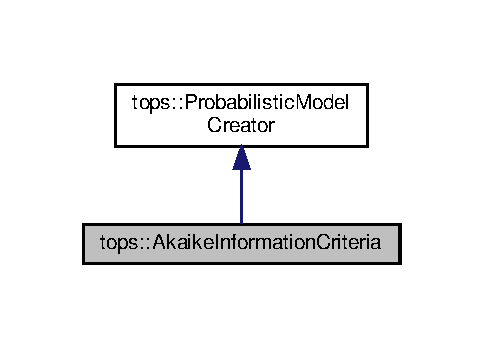
\includegraphics[width=232pt]{classtops_1_1AkaikeInformationCriteria__inherit__graph}
\end{center}
\end{figure}


Collaboration diagram for tops\+:\+:Akaike\+Information\+Criteria\+:
\nopagebreak
\begin{figure}[H]
\begin{center}
\leavevmode
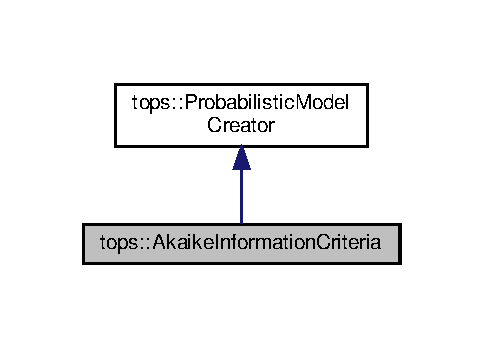
\includegraphics[width=232pt]{classtops_1_1AkaikeInformationCriteria__coll__graph}
\end{center}
\end{figure}
\subsection*{Public Member Functions}
\begin{DoxyCompactItemize}
\item 
\mbox{\Hypertarget{classtops_1_1AkaikeInformationCriteria_a49e40b8fa596e3185f3a12caca7b4201}\label{classtops_1_1AkaikeInformationCriteria_a49e40b8fa596e3185f3a12caca7b4201}} 
{\bfseries Akaike\+Information\+Criteria} (Probabilistic\+Model\+Creator\+Ptr creator)
\item 
virtual Probabilistic\+Model\+Ptr \hyperlink{classtops_1_1AkaikeInformationCriteria_a925de08fa8373de8f7ddf48cd6b2c6e0}{create} (\hyperlink{classtops_1_1ProbabilisticModelParameters}{Probabilistic\+Model\+Parameters} \&parameters) const
\begin{DoxyCompactList}\small\item\em Creates a new model using the received parameters. \end{DoxyCompactList}\item 
\mbox{\Hypertarget{classtops_1_1AkaikeInformationCriteria_ab0460e83a273c2e87f5009bd3a1177fd}\label{classtops_1_1AkaikeInformationCriteria_ab0460e83a273c2e87f5009bd3a1177fd}} 
virtual std\+::string \hyperlink{classtops_1_1AkaikeInformationCriteria_ab0460e83a273c2e87f5009bd3a1177fd}{help} () const
\begin{DoxyCompactList}\small\item\em returns a help message of this creator \end{DoxyCompactList}\item 
\mbox{\Hypertarget{classtops_1_1AkaikeInformationCriteria_a5294784ba6eaa8ba35c7f21b9bcedc70}\label{classtops_1_1AkaikeInformationCriteria_a5294784ba6eaa8ba35c7f21b9bcedc70}} 
virtual void \hyperlink{classtops_1_1AkaikeInformationCriteria_a5294784ba6eaa8ba35c7f21b9bcedc70}{set\+Creator} (Probabilistic\+Model\+Creator\+Ptr creator)
\begin{DoxyCompactList}\small\item\em Set a creator. \end{DoxyCompactList}\end{DoxyCompactItemize}


\subsection{Detailed Description}
This class implements the Akaike Information Criteria. 

Definition at line 38 of file Akaike\+Information\+Criteria.\+hpp.



\subsection{Member Function Documentation}
\mbox{\Hypertarget{classtops_1_1AkaikeInformationCriteria_a925de08fa8373de8f7ddf48cd6b2c6e0}\label{classtops_1_1AkaikeInformationCriteria_a925de08fa8373de8f7ddf48cd6b2c6e0}} 
\index{tops\+::\+Akaike\+Information\+Criteria@{tops\+::\+Akaike\+Information\+Criteria}!create@{create}}
\index{create@{create}!tops\+::\+Akaike\+Information\+Criteria@{tops\+::\+Akaike\+Information\+Criteria}}
\subsubsection{\texorpdfstring{create()}{create()}}
{\footnotesize\ttfamily Probabilistic\+Model\+Ptr tops\+::\+Akaike\+Information\+Criteria\+::create (\begin{DoxyParamCaption}\item[{\hyperlink{classtops_1_1ProbabilisticModelParameters}{Probabilistic\+Model\+Parameters} \&}]{parameters }\end{DoxyParamCaption}) const\hspace{0.3cm}{\ttfamily [virtual]}}



Creates a new model using the received parameters. 


\begin{DoxyParams}{Parameters}
{\em parameters} & of the model\textquotesingle{}s creator \\
\hline
\end{DoxyParams}
\begin{DoxyReturn}{Returns}
An instance of \hyperlink{classtops_1_1ProbabilisticModel}{Probabilistic\+Model} 
\end{DoxyReturn}


Reimplemented from \hyperlink{classtops_1_1ProbabilisticModelCreator_afed6c8ffa45fff446bdaa8b533da8f7c}{tops\+::\+Probabilistic\+Model\+Creator}.



Definition at line 55 of file Akaike\+Information\+Criteria.\+cpp.


\begin{DoxyCode}
56   \{
57     ProbabilisticModelParameterValuePtr beginpar = parameters.getMandatoryParameterValue(\textcolor{stringliteral}{"begin"});
58     ProbabilisticModelParameterValuePtr endpar = parameters.getMandatoryParameterValue(\textcolor{stringliteral}{"end"});
59     ProbabilisticModelParameterValuePtr steppar = parameters.getMandatoryParameterValue(\textcolor{stringliteral}{"step"});
60     ProbabilisticModelParameterValuePtr trainpar = parameters.getMandatoryParameterValue(\textcolor{stringliteral}{"
      training\_algorithm"});
61 
62     \textcolor{keywordflow}{if}((beginpar == NULL) ||
63        (endpar == NULL) ||
64        (steppar == NULL))
65       \{
66         std::cerr << \hyperlink{classtops_1_1AkaikeInformationCriteria_ab0460e83a273c2e87f5009bd3a1177fd}{help}() << std::endl;
67         exit(-1);
68       \}
69     std::map<std::string, double> beginmap = beginpar->getDoubleMap();
70     std::map<std::string, double> endmap = endpar->getDoubleMap();
71     std::map<std::string, double> stepmap = steppar->getDoubleMap();
72     std::vector <std::string> parnames;
73     std::map <std::string, double>::const\_iterator it;
74     \textcolor{keywordflow}{for}(it = beginmap.begin(); it!=beginmap.end(); it++)
75       parnames.push\_back(it->first);
76 
77     \textcolor{comment}{// generates all possible combinations of parameters}
78     std::vector <std::string>::const\_iterator p;
79     std::vector <std::vector <double> > combinations;
80     combinations.resize(1);
81     \textcolor{keywordflow}{for}(p = parnames.begin(); p != parnames.end(); p++)
82       \{
83         std::vector <std::vector <double> > new\_combinations;
84         \textcolor{keywordflow}{for} (\textcolor{keywordtype}{double} i = beginmap[*p] ; i <= endmap[*p]; i += stepmap[*p])
85           \{
86             \textcolor{keywordflow}{for}(\textcolor{keywordtype}{int} j = 0; j < (int) combinations.size() ; j++)
87               \{
88                 std::vector <double> comb;
89                 \textcolor{keywordflow}{for}(\textcolor{keywordtype}{int} k = 0; k < (int)combinations[j].size(); k++)
90                   comb.push\_back(combinations[j][k]);
91                 comb.push\_back(i);
92                 new\_combinations.push\_back(comb);
93               \}
94           \}
95         combinations = new\_combinations;
96       \}
97     \textcolor{keywordtype}{double} aic = HUGE;
98     ProbabilisticModelPtr result;
99     \textcolor{keywordflow}{for}(\textcolor{keywordtype}{int} i = 0; i < (int) combinations.size(); i++)
100       \{
101         \textcolor{keywordflow}{for}(\textcolor{keywordtype}{int} j = 0; j < (int) combinations[i].size(); j++)
102           \{
103             DoubleParameterValuePtr value = DoubleParameterValuePtr(\textcolor{keyword}{new} DoubleParameterValue(combinations[i
      ][j]));
104 
105             parameters.set(parnames[j], value);
106           \}
107         \textcolor{keywordtype}{double} loglikelihood;
108         \textcolor{keywordtype}{int} sample\_size;
109         ProbabilisticModelPtr m = \_creator->create(parameters, loglikelihood, sample\_size);
110         \textcolor{keywordtype}{double} model\_aic = 2 * m->size()  - 2* loglikelihood ;
111         \textcolor{keywordflow}{if}(aic > model\_aic)
112           \{
113             aic = model\_aic;
114             result = m;
115           \}
116 
117         \textcolor{keywordtype}{int} k = 0;
118         \textcolor{keywordflow}{if}( k < (\textcolor{keywordtype}{int}) combinations[i].size())
119           \{
120             std::cerr << combinations[i][k];
121             \textcolor{keywordflow}{for}(k = 1; k < (int) combinations[i].size(); k++)
122               std::cerr << \textcolor{stringliteral}{"\(\backslash\)t"} << combinations[i][k];
123           \}
124         std::cerr << \textcolor{stringliteral}{"\(\backslash\)t"} << model\_aic  << std::endl;
125 
126       \}
127     std::cout << \textcolor{stringliteral}{"# Model AIC: "} << aic  << std::endl;
128     \textcolor{keywordflow}{return} result;
129   \}
\end{DoxyCode}


The documentation for this class was generated from the following files\+:\begin{DoxyCompactItemize}
\item 
src/Akaike\+Information\+Criteria.\+hpp\item 
src/Akaike\+Information\+Criteria.\+cpp\end{DoxyCompactItemize}

\hypertarget{classtops_1_1Alphabet}{}\section{tops\+:\+:Alphabet Class Reference}
\label{classtops_1_1Alphabet}\index{tops\+::\+Alphabet@{tops\+::\+Alphabet}}


A class representing \hyperlink{classtops_1_1Alphabet}{Alphabet}.  




{\ttfamily \#include $<$Alphabet.\+hpp$>$}

\subsection*{Public Member Functions}
\begin{DoxyCompactItemize}
\item 
Symbol\+Ptr \hyperlink{classtops_1_1Alphabet_ae82947c05a15225d90a93547d26c10b0}{create\+Symbol} (const std\+::string \&name)
\begin{DoxyCompactList}\small\item\em Creates a new symbol. \end{DoxyCompactList}\item 
\mbox{\Hypertarget{classtops_1_1Alphabet_a559fdaf75922ccb4927ad868822c9305}\label{classtops_1_1Alphabet_a559fdaf75922ccb4927ad868822c9305}} 
Symbol\+Ptr {\bfseries create\+Symbol} (char $\ast$name)
\item 
\mbox{\Hypertarget{classtops_1_1Alphabet_ad72e398ac3123f76c978e3c41e61e959}\label{classtops_1_1Alphabet_ad72e398ac3123f76c978e3c41e61e959}} 
unsigned int \hyperlink{classtops_1_1Alphabet_ad72e398ac3123f76c978e3c41e61e959}{max\+Symbol\+Size} ()
\begin{DoxyCompactList}\small\item\em Returns the maximum length of the symbol. \end{DoxyCompactList}\item 
\mbox{\Hypertarget{classtops_1_1Alphabet_a0ecfdfad56bda227522acb504b20c20e}\label{classtops_1_1Alphabet_a0ecfdfad56bda227522acb504b20c20e}} 
unsigned int \hyperlink{classtops_1_1Alphabet_a0ecfdfad56bda227522acb504b20c20e}{size} ()
\begin{DoxyCompactList}\small\item\em Returns the alphabet size. \end{DoxyCompactList}\item 
\mbox{\Hypertarget{classtops_1_1Alphabet_ada9bbe4368c00ca714b99ba49bd9d350}\label{classtops_1_1Alphabet_ada9bbe4368c00ca714b99ba49bd9d350}} 
Symbol\+Ptr \hyperlink{classtops_1_1Alphabet_ada9bbe4368c00ca714b99ba49bd9d350}{get\+Symbol} (int k)
\begin{DoxyCompactList}\small\item\em Returns the symbol given an id. \end{DoxyCompactList}\item 
\mbox{\Hypertarget{classtops_1_1Alphabet_a74ceff8279639cdafc261e70bb37f6ea}\label{classtops_1_1Alphabet_a74ceff8279639cdafc261e70bb37f6ea}} 
Symbol\+Ptr \hyperlink{classtops_1_1Alphabet_a74ceff8279639cdafc261e70bb37f6ea}{get\+Symbol} (const std\+::string \&s)
\begin{DoxyCompactList}\small\item\em Get the symbol given the symbol name. \end{DoxyCompactList}\item 
bool \hyperlink{classtops_1_1Alphabet_af41f8fcef3a5e540a8af63afc85df668}{has} (const std\+::string \&s)
\begin{DoxyCompactList}\small\item\em Returns true if the symbol name s is in the \hyperlink{classtops_1_1Alphabet}{Alphabet}. \end{DoxyCompactList}\item 
\mbox{\Hypertarget{classtops_1_1Alphabet_ab0d2d98fe0612f204aaf59e6e18f7c8b}\label{classtops_1_1Alphabet_ab0d2d98fe0612f204aaf59e6e18f7c8b}} 
void \hyperlink{classtops_1_1Alphabet_ab0d2d98fe0612f204aaf59e6e18f7c8b}{initialize\+From\+Vector} (const std\+::vector$<$ std\+::string $>$ \&\hyperlink{classtops_1_1Alphabet_a85e599e3d65ffc47e3588c887fa2da95}{str})
\begin{DoxyCompactList}\small\item\em Initialize the alphabet using a list of symbols. \end{DoxyCompactList}\item 
\mbox{\Hypertarget{classtops_1_1Alphabet_a85e599e3d65ffc47e3588c887fa2da95}\label{classtops_1_1Alphabet_a85e599e3d65ffc47e3588c887fa2da95}} 
std\+::string \hyperlink{classtops_1_1Alphabet_a85e599e3d65ffc47e3588c887fa2da95}{str} () const
\begin{DoxyCompactList}\small\item\em String representation of this alphabet. \end{DoxyCompactList}\item 
\mbox{\Hypertarget{classtops_1_1Alphabet_a3afc3b5cc761fcfb896839ac07b8144c}\label{classtops_1_1Alphabet_a3afc3b5cc761fcfb896839ac07b8144c}} 
Probabilistic\+Model\+Parameter\+Value\+Ptr {\bfseries get\+Parameter\+Value} ()
\end{DoxyCompactItemize}


\subsection{Detailed Description}
A class representing \hyperlink{classtops_1_1Alphabet}{Alphabet}. 

Definition at line 48 of file Alphabet.\+hpp.



\subsection{Member Function Documentation}
\mbox{\Hypertarget{classtops_1_1Alphabet_ae82947c05a15225d90a93547d26c10b0}\label{classtops_1_1Alphabet_ae82947c05a15225d90a93547d26c10b0}} 
\index{tops\+::\+Alphabet@{tops\+::\+Alphabet}!create\+Symbol@{create\+Symbol}}
\index{create\+Symbol@{create\+Symbol}!tops\+::\+Alphabet@{tops\+::\+Alphabet}}
\subsubsection{\texorpdfstring{create\+Symbol()}{createSymbol()}}
{\footnotesize\ttfamily Symbol\+Ptr tops\+::\+Alphabet\+::create\+Symbol (\begin{DoxyParamCaption}\item[{const std\+::string \&}]{name }\end{DoxyParamCaption})}



Creates a new symbol. 


\begin{DoxyParams}{Parameters}
{\em name} & is the symbol name \\
\hline
\end{DoxyParams}


Definition at line 101 of file Alphabet.\+cpp.


\begin{DoxyCode}
102   \{
103     \textcolor{keywordtype}{int} i;
104     \textcolor{keywordflow}{if} (name.size() > \_max\_symbol\_size) 
105       \_max\_symbol\_size = name.size();
106     \textcolor{keywordflow}{for}(i = 0; i < (int)\_pool.size(); i++)
107       \textcolor{keywordflow}{if}(\_pool[i]->name() == name)
108         \textcolor{keywordflow}{return} \hyperlink{classtops_1_1Alphabet_ada9bbe4368c00ca714b99ba49bd9d350}{getSymbol}(i);
109     SymbolPtr s = SymbolPtr( \textcolor{keyword}{new} Symbol(i, name, \textcolor{keyword}{this}));
110     \_stringToSymbol[name] = s;
111     \_pool.push\_back(s);
112     \textcolor{keywordflow}{return} \hyperlink{classtops_1_1Alphabet_ada9bbe4368c00ca714b99ba49bd9d350}{getSymbol}(i);
113   \}
\end{DoxyCode}
\mbox{\Hypertarget{classtops_1_1Alphabet_af41f8fcef3a5e540a8af63afc85df668}\label{classtops_1_1Alphabet_af41f8fcef3a5e540a8af63afc85df668}} 
\index{tops\+::\+Alphabet@{tops\+::\+Alphabet}!has@{has}}
\index{has@{has}!tops\+::\+Alphabet@{tops\+::\+Alphabet}}
\subsubsection{\texorpdfstring{has()}{has()}}
{\footnotesize\ttfamily bool tops\+::\+Alphabet\+::has (\begin{DoxyParamCaption}\item[{const std\+::string \&}]{s }\end{DoxyParamCaption})}



Returns true if the symbol name s is in the \hyperlink{classtops_1_1Alphabet}{Alphabet}. 


\begin{DoxyParams}{Parameters}
{\em s} & is the name of the symbol \\
\hline
\end{DoxyParams}
\begin{DoxyReturn}{Returns}
true if the name of the symbol is in the \hyperlink{classtops_1_1Alphabet}{Alphabet} 
\end{DoxyReturn}


Definition at line 34 of file Alphabet.\+cpp.


\begin{DoxyCode}
35   \{
36     std::map<std::string, SymbolPtr>::iterator it;
37     it = \_stringToSymbol.find(s);
38     \textcolor{keywordflow}{return} it != \_stringToSymbol.end();
39   \}
\end{DoxyCode}


The documentation for this class was generated from the following files\+:\begin{DoxyCompactItemize}
\item 
src/Alphabet.\+hpp\item 
src/Alphabet.\+cpp\end{DoxyCompactItemize}

\hypertarget{classtops_1_1BayesianInformationCriteria}{}\section{tops\+:\+:Bayesian\+Information\+Criteria Class Reference}
\label{classtops_1_1BayesianInformationCriteria}\index{tops\+::\+Bayesian\+Information\+Criteria@{tops\+::\+Bayesian\+Information\+Criteria}}


Bayesian Information Criteria.  




{\ttfamily \#include $<$Bayesian\+Information\+Criteria.\+hpp$>$}



Inheritance diagram for tops\+:\+:Bayesian\+Information\+Criteria\+:
\nopagebreak
\begin{figure}[H]
\begin{center}
\leavevmode
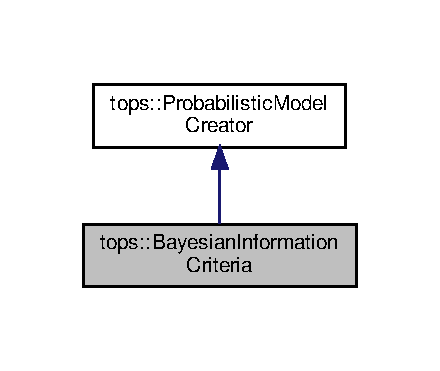
\includegraphics[width=211pt]{classtops_1_1BayesianInformationCriteria__inherit__graph}
\end{center}
\end{figure}


Collaboration diagram for tops\+:\+:Bayesian\+Information\+Criteria\+:
\nopagebreak
\begin{figure}[H]
\begin{center}
\leavevmode
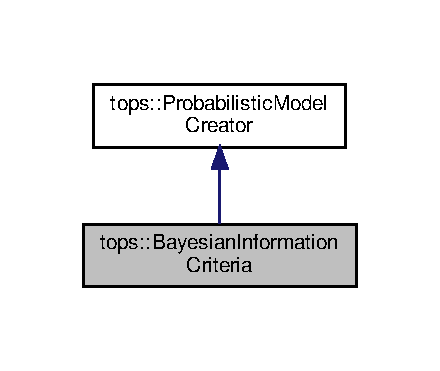
\includegraphics[width=211pt]{classtops_1_1BayesianInformationCriteria__coll__graph}
\end{center}
\end{figure}
\subsection*{Public Member Functions}
\begin{DoxyCompactItemize}
\item 
\mbox{\Hypertarget{classtops_1_1BayesianInformationCriteria_ada34ed0f999f017e91a2b5039e75ed42}\label{classtops_1_1BayesianInformationCriteria_ada34ed0f999f017e91a2b5039e75ed42}} 
{\bfseries Bayesian\+Information\+Criteria} (Probabilistic\+Model\+Creator\+Ptr creator)
\item 
virtual Probabilistic\+Model\+Ptr \hyperlink{classtops_1_1BayesianInformationCriteria_a025c7fff02580703f901376eea7db340}{create} (\hyperlink{classtops_1_1ProbabilisticModelParameters}{Probabilistic\+Model\+Parameters} \&parameters) const
\begin{DoxyCompactList}\small\item\em Creates a new model using the received parameters. \end{DoxyCompactList}\item 
\mbox{\Hypertarget{classtops_1_1BayesianInformationCriteria_ab420897d48ca999b1f8b236cef896b5b}\label{classtops_1_1BayesianInformationCriteria_ab420897d48ca999b1f8b236cef896b5b}} 
virtual std\+::string \hyperlink{classtops_1_1BayesianInformationCriteria_ab420897d48ca999b1f8b236cef896b5b}{help} () const
\begin{DoxyCompactList}\small\item\em Returns a help message of this creator. \end{DoxyCompactList}\item 
\mbox{\Hypertarget{classtops_1_1BayesianInformationCriteria_a941f1105ec71881d8b30125047374467}\label{classtops_1_1BayesianInformationCriteria_a941f1105ec71881d8b30125047374467}} 
virtual void \hyperlink{classtops_1_1BayesianInformationCriteria_a941f1105ec71881d8b30125047374467}{set\+Creator} (Probabilistic\+Model\+Creator\+Ptr creator)
\begin{DoxyCompactList}\small\item\em Set a creator. \end{DoxyCompactList}\end{DoxyCompactItemize}


\subsection{Detailed Description}
Bayesian Information Criteria. 

Definition at line 37 of file Bayesian\+Information\+Criteria.\+hpp.



\subsection{Member Function Documentation}
\mbox{\Hypertarget{classtops_1_1BayesianInformationCriteria_a025c7fff02580703f901376eea7db340}\label{classtops_1_1BayesianInformationCriteria_a025c7fff02580703f901376eea7db340}} 
\index{tops\+::\+Bayesian\+Information\+Criteria@{tops\+::\+Bayesian\+Information\+Criteria}!create@{create}}
\index{create@{create}!tops\+::\+Bayesian\+Information\+Criteria@{tops\+::\+Bayesian\+Information\+Criteria}}
\subsubsection{\texorpdfstring{create()}{create()}}
{\footnotesize\ttfamily Probabilistic\+Model\+Ptr tops\+::\+Bayesian\+Information\+Criteria\+::create (\begin{DoxyParamCaption}\item[{\hyperlink{classtops_1_1ProbabilisticModelParameters}{Probabilistic\+Model\+Parameters} \&}]{parameters }\end{DoxyParamCaption}) const\hspace{0.3cm}{\ttfamily [virtual]}}



Creates a new model using the received parameters. 


\begin{DoxyParams}{Parameters}
{\em parameters} & of the model\textquotesingle{}s creators \\
\hline
\end{DoxyParams}
\begin{DoxyReturn}{Returns}
An instance of \hyperlink{classtops_1_1ProbabilisticModel}{Probabilistic\+Model} 
\end{DoxyReturn}


Reimplemented from \hyperlink{classtops_1_1ProbabilisticModelCreator_afed6c8ffa45fff446bdaa8b533da8f7c}{tops\+::\+Probabilistic\+Model\+Creator}.



Definition at line 53 of file Bayesian\+Information\+Criteria.\+cpp.


\begin{DoxyCode}
54   \{
55     ProbabilisticModelParameterValuePtr beginpar = parameters.getMandatoryParameterValue(\textcolor{stringliteral}{"begin"});
56     ProbabilisticModelParameterValuePtr endpar = parameters.getMandatoryParameterValue(\textcolor{stringliteral}{"end"});
57     ProbabilisticModelParameterValuePtr steppar = parameters.getMandatoryParameterValue(\textcolor{stringliteral}{"step"});
58     ProbabilisticModelParameterValuePtr trainpar = parameters.getMandatoryParameterValue(\textcolor{stringliteral}{"
      training\_algorithm"});
59 
60     \textcolor{keywordflow}{if}((beginpar == NULL) ||
61        (endpar == NULL) ||
62        (steppar == NULL))
63       \{
64         std::cerr << \hyperlink{classtops_1_1BayesianInformationCriteria_ab420897d48ca999b1f8b236cef896b5b}{help}() << std::endl;
65         exit(-1);
66       \}
67     std::map<std::string, double> beginmap = beginpar->getDoubleMap();
68     std::map<std::string, double> endmap = endpar->getDoubleMap();
69     std::map<std::string, double> stepmap = steppar->getDoubleMap();
70     std::vector <std::string> parnames;
71     std::map <std::string, double>::const\_iterator it;
72     \textcolor{keywordflow}{for}(it = beginmap.begin(); it!=beginmap.end(); it++)
73       parnames.push\_back(it->first);
74 
75     \textcolor{comment}{// generates all possible combinations of parameters}
76     std::vector <std::string>::const\_iterator p;
77     std::vector <std::vector <double> > combinations;
78     combinations.resize(1);
79     \textcolor{keywordflow}{for}(p = parnames.begin(); p != parnames.end(); p++)
80       \{
81         std::vector <std::vector <double> > new\_combinations;
82         \textcolor{keywordflow}{for} (\textcolor{keywordtype}{double} i = beginmap[*p] ; i <= endmap[*p]; i += stepmap[*p])
83           \{
84             \textcolor{keywordflow}{for}(\textcolor{keywordtype}{int} j = 0; j < (int) combinations.size() ; j++)
85               \{
86                 std::vector <double> comb;
87                 \textcolor{keywordflow}{for}(\textcolor{keywordtype}{int} k = 0; k < (int)combinations[j].size(); k++)
88                   comb.push\_back(combinations[j][k]);
89                 comb.push\_back(i);
90                 new\_combinations.push\_back(comb);
91               \}
92           \}
93         combinations = new\_combinations;
94       \}
95     \textcolor{keywordtype}{double} bic = -HUGE;
96     ProbabilisticModelPtr result;
97     \textcolor{keywordflow}{for}(\textcolor{keywordtype}{int} i = 0; i < (int) combinations.size(); i++)
98       \{
99         \textcolor{keywordflow}{for}(\textcolor{keywordtype}{int} j = 0; j < (int) combinations[i].size(); j++)
100           \{
101             DoubleParameterValuePtr value = DoubleParameterValuePtr(\textcolor{keyword}{new} DoubleParameterValue(combinations[i
      ][j]));
102 
103             parameters.set(parnames[j], value);
104           \}
105         \textcolor{keywordtype}{double} loglikelihood;
106         \textcolor{keywordtype}{int} sample\_size;
107         ProbabilisticModelPtr m = \_creator->create(parameters, loglikelihood, sample\_size);
108         \textcolor{keywordflow}{if}(m == NULL)
109             \{
110                 std::cerr << \textcolor{stringliteral}{"ERROR (BIC): could not estimate the model size using BIC "} << std::endl;
111                 exit(-1);
112             \}
113         \textcolor{keywordtype}{double} model\_bic =  loglikelihood  - 0.5* m->size() * log((\textcolor{keywordtype}{double}) sample\_size);
114         \textcolor{keywordflow}{if}((bic < model\_bic) || (result == NULL))
115           \{
116             bic = model\_bic;
117             result = m;
118           \}
119 
120         \textcolor{keywordtype}{int} k = 0;
121         \textcolor{keywordflow}{if}( k < (\textcolor{keywordtype}{int}) combinations[i].size())
122           \{
123             std::cerr << combinations[i][k];
124             \textcolor{keywordflow}{for}(k = 1; k < (int) combinations[i].size(); k++)
125               std::cerr << \textcolor{stringliteral}{"\(\backslash\)t"} << combinations[i][k];
126           \}
127         std::cerr << \textcolor{stringliteral}{"\(\backslash\)t"} << model\_bic  << std::endl;
128 
129       \}
130     std::cout << \textcolor{stringliteral}{"# Model BIC: "} << bic  << std::endl;
131     \textcolor{keywordflow}{return} result;
132   \}
\end{DoxyCode}


The documentation for this class was generated from the following files\+:\begin{DoxyCompactItemize}
\item 
src/Bayesian\+Information\+Criteria.\+hpp\item 
src/Bayesian\+Information\+Criteria.\+cpp\end{DoxyCompactItemize}

\hypertarget{classtops_1_1BernoulliModelCreator}{}\section{tops\+:\+:Bernoulli\+Model\+Creator Class Reference}
\label{classtops_1_1BernoulliModelCreator}\index{tops\+::\+Bernoulli\+Model\+Creator@{tops\+::\+Bernoulli\+Model\+Creator}}


This class is a factory for the bernoulli distribution.  




{\ttfamily \#include $<$Bernoulli\+Model\+Creator.\+hpp$>$}



Inheritance diagram for tops\+:\+:Bernoulli\+Model\+Creator\+:
\nopagebreak
\begin{figure}[H]
\begin{center}
\leavevmode
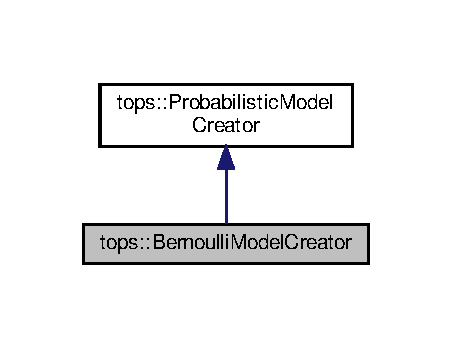
\includegraphics[width=217pt]{classtops_1_1BernoulliModelCreator__inherit__graph}
\end{center}
\end{figure}


Collaboration diagram for tops\+:\+:Bernoulli\+Model\+Creator\+:
\nopagebreak
\begin{figure}[H]
\begin{center}
\leavevmode
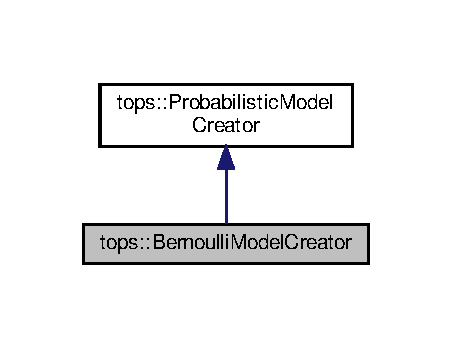
\includegraphics[width=217pt]{classtops_1_1BernoulliModelCreator__coll__graph}
\end{center}
\end{figure}
\subsection*{Public Member Functions}
\begin{DoxyCompactItemize}
\item 
virtual Probabilistic\+Model\+Ptr \hyperlink{classtops_1_1BernoulliModelCreator_a7269fc3cbc7bef0bc7456e6cf2ec44b3}{create} (\hyperlink{classtops_1_1ProbabilisticModelParameters}{Probabilistic\+Model\+Parameters} \&parameters) const
\begin{DoxyCompactList}\small\item\em Creates a probabilistic model. \end{DoxyCompactList}\item 
\mbox{\Hypertarget{classtops_1_1BernoulliModelCreator_a7b95b973ccc98192f835e98b656cd6ee}\label{classtops_1_1BernoulliModelCreator_a7b95b973ccc98192f835e98b656cd6ee}} 
virtual std\+::string \hyperlink{classtops_1_1BernoulliModelCreator_a7b95b973ccc98192f835e98b656cd6ee}{help} () const
\begin{DoxyCompactList}\small\item\em This method returns a help message. \end{DoxyCompactList}\end{DoxyCompactItemize}


\subsection{Detailed Description}
This class is a factory for the bernoulli distribution. 

Definition at line 36 of file Bernoulli\+Model\+Creator.\+hpp.



\subsection{Member Function Documentation}
\mbox{\Hypertarget{classtops_1_1BernoulliModelCreator_a7269fc3cbc7bef0bc7456e6cf2ec44b3}\label{classtops_1_1BernoulliModelCreator_a7269fc3cbc7bef0bc7456e6cf2ec44b3}} 
\index{tops\+::\+Bernoulli\+Model\+Creator@{tops\+::\+Bernoulli\+Model\+Creator}!create@{create}}
\index{create@{create}!tops\+::\+Bernoulli\+Model\+Creator@{tops\+::\+Bernoulli\+Model\+Creator}}
\subsubsection{\texorpdfstring{create()}{create()}}
{\footnotesize\ttfamily Probabilistic\+Model\+Ptr tops\+::\+Bernoulli\+Model\+Creator\+::create (\begin{DoxyParamCaption}\item[{\hyperlink{classtops_1_1ProbabilisticModelParameters}{Probabilistic\+Model\+Parameters} \&}]{parameters }\end{DoxyParamCaption}) const\hspace{0.3cm}{\ttfamily [virtual]}}



Creates a probabilistic model. 


\begin{DoxyParams}{Parameters}
{\em parameters} & is a set of parameters that is utilized to build the model \\
\hline
\end{DoxyParams}


Reimplemented from \hyperlink{classtops_1_1ProbabilisticModelCreator_afed6c8ffa45fff446bdaa8b533da8f7c}{tops\+::\+Probabilistic\+Model\+Creator}.



Definition at line 31 of file Bernoulli\+Model\+Creator.\+cpp.


\begin{DoxyCode}
31                                                                                                      \{
32     ProbabilisticModelParameterValuePtr probs = parameters.getMandatoryParameterValue(\textcolor{stringliteral}{"probability"});
33     \textcolor{keywordflow}{if}(probs == NULL)
34       \{
35         std::cerr << \hyperlink{classtops_1_1BernoulliModelCreator_a7b95b973ccc98192f835e98b656cd6ee}{help}() << std::endl;
36         exit(-1);
37       \}
38     DoubleVector distr;
39     distr.push\_back(probs->getDouble());
40     distr.push\_back(1.0 - probs->getDouble());
41     ProbabilisticModelPtr model = DiscreteIIDModelPtr(\textcolor{keyword}{new} DiscreteIIDModel(distr));
42     \textcolor{keywordflow}{return} model;
43   \}
\end{DoxyCode}


The documentation for this class was generated from the following files\+:\begin{DoxyCompactItemize}
\item 
src/Bernoulli\+Model\+Creator.\+hpp\item 
src/Bernoulli\+Model\+Creator.\+cpp\end{DoxyCompactItemize}

\hypertarget{structtops_1_1column}{}\section{tops\+:\+:column Struct Reference}
\label{structtops_1_1column}\index{tops\+::column@{tops\+::column}}
\subsection*{Public Attributes}
\begin{DoxyCompactItemize}
\item 
\mbox{\Hypertarget{structtops_1_1column_aa6801c7b9432897cff4d48351c0d73f3}\label{structtops_1_1column_aa6801c7b9432897cff4d48351c0d73f3}} 
int {\bfseries index}
\item 
\mbox{\Hypertarget{structtops_1_1column_a8a72f7e3662ead6cb59ec8350c3ee739}\label{structtops_1_1column_a8a72f7e3662ead6cb59ec8350c3ee739}} 
bool {\bfseries visited}
\item 
\mbox{\Hypertarget{structtops_1_1column_af8959eab97e757afaf9e1942f2d93ae6}\label{structtops_1_1column_af8959eab97e757afaf9e1942f2d93ae6}} 
bool {\bfseries is\+Dead}
\item 
\mbox{\Hypertarget{structtops_1_1column_af442f0129b61e6bfeac37984fba0e100}\label{structtops_1_1column_af442f0129b61e6bfeac37984fba0e100}} 
vector$<$ seq\+Pos $>$ {\bfseries col\+Seq\+Pos}
\end{DoxyCompactItemize}


\subsection{Detailed Description}


Definition at line 27 of file Multiple\+Alignment.\+hpp.



The documentation for this struct was generated from the following file\+:\begin{DoxyCompactItemize}
\item 
src/Multiple\+Alignment.\+hpp\end{DoxyCompactItemize}

\hypertarget{classtops_1_1ConfigurationReader}{}\section{tops\+:\+:Configuration\+Reader Class Reference}
\label{classtops_1_1ConfigurationReader}\index{tops\+::\+Configuration\+Reader@{tops\+::\+Configuration\+Reader}}


This class reads a configuration file.  




{\ttfamily \#include $<$Configuration\+Reader.\+hpp$>$}

\subsection*{Public Member Functions}
\begin{DoxyCompactItemize}
\item 
\mbox{\Hypertarget{classtops_1_1ConfigurationReader_a148538236b5a821dfcc44feef99a5dc1}\label{classtops_1_1ConfigurationReader_a148538236b5a821dfcc44feef99a5dc1}} 
bool \hyperlink{classtops_1_1ConfigurationReader_a148538236b5a821dfcc44feef99a5dc1}{load} (std\+::string \&data)
\begin{DoxyCompactList}\small\item\em Loads the configuration from the data string. \end{DoxyCompactList}\item 
\mbox{\Hypertarget{classtops_1_1ConfigurationReader_a830b793b186f7e9fe17bc00eff16e7f1}\label{classtops_1_1ConfigurationReader_a830b793b186f7e9fe17bc00eff16e7f1}} 
bool \hyperlink{classtops_1_1ConfigurationReader_a830b793b186f7e9fe17bc00eff16e7f1}{load\+From\+File} (const std\+::string \&filename)
\begin{DoxyCompactList}\small\item\em Loads the configuration from a file. \end{DoxyCompactList}\item 
\mbox{\Hypertarget{classtops_1_1ConfigurationReader_a83e683d2e79cf6de5c4e7c617302c786}\label{classtops_1_1ConfigurationReader_a83e683d2e79cf6de5c4e7c617302c786}} 
void {\bfseries set\+Current\+Parameter\+Value} (Probabilistic\+Model\+Parameter\+Value\+Ptr value)
\item 
\mbox{\Hypertarget{classtops_1_1ConfigurationReader_ab12d621df5a3caf48f5e1981a2d2d23c}\label{classtops_1_1ConfigurationReader_ab12d621df5a3caf48f5e1981a2d2d23c}} 
Probabilistic\+Model\+Parameter\+Value\+Ptr {\bfseries get\+Current\+Parameter\+Value} ()
\item 
\mbox{\Hypertarget{classtops_1_1ConfigurationReader_af49b5bdb58a47c5bb1a398ad89168a2e}\label{classtops_1_1ConfigurationReader_af49b5bdb58a47c5bb1a398ad89168a2e}} 
void {\bfseries set\+Current\+Parameter\+Name} (const std\+::string \&name)
\item 
\mbox{\Hypertarget{classtops_1_1ConfigurationReader_a8624fe6b02112a60e5f3c7542efc91aa}\label{classtops_1_1ConfigurationReader_a8624fe6b02112a60e5f3c7542efc91aa}} 
void {\bfseries set\+Aux\+String} (const std\+::string \&aux)
\item 
\mbox{\Hypertarget{classtops_1_1ConfigurationReader_a36e5cc1447a21428ab2628902d22c42b}\label{classtops_1_1ConfigurationReader_a36e5cc1447a21428ab2628902d22c42b}} 
std\+::string {\bfseries get\+Aux\+String} ()
\item 
\mbox{\Hypertarget{classtops_1_1ConfigurationReader_afa314d7735d36bea1a12ae6bb26ec1d8}\label{classtops_1_1ConfigurationReader_afa314d7735d36bea1a12ae6bb26ec1d8}} 
std\+::string {\bfseries get\+Current\+Parameter\+Name} ()
\item 
\mbox{\Hypertarget{classtops_1_1ConfigurationReader_ac8e03c9cdc40def083259aa12f34cdc0}\label{classtops_1_1ConfigurationReader_ac8e03c9cdc40def083259aa12f34cdc0}} 
void {\bfseries add\+\_\+parameter} ()
\item 
\mbox{\Hypertarget{classtops_1_1ConfigurationReader_a0aa802b5da8aeb58aba4efc545605f96}\label{classtops_1_1ConfigurationReader_a0aa802b5da8aeb58aba4efc545605f96}} 
Probabilistic\+Model\+Parameters\+Ptr {\bfseries parameters} ()
\item 
\mbox{\Hypertarget{classtops_1_1ConfigurationReader_a62a3e63f200aaab2bc40632e9f72901a}\label{classtops_1_1ConfigurationReader_a62a3e63f200aaab2bc40632e9f72901a}} 
std\+::string {\bfseries get\+Aux\+String2} ()
\item 
\mbox{\Hypertarget{classtops_1_1ConfigurationReader_ab99963ac7f054d76ebbc460414d42b2a}\label{classtops_1_1ConfigurationReader_ab99963ac7f054d76ebbc460414d42b2a}} 
std\+::string {\bfseries get\+Aux\+String3} ()
\item 
\mbox{\Hypertarget{classtops_1_1ConfigurationReader_a2871b540b10ca59481aba23376cb1956}\label{classtops_1_1ConfigurationReader_a2871b540b10ca59481aba23376cb1956}} 
void {\bfseries set\+Aux\+String2} (const std\+::string \&aux)
\item 
\mbox{\Hypertarget{classtops_1_1ConfigurationReader_aee34b8155b6073c5f5a71ba0566fa9f2}\label{classtops_1_1ConfigurationReader_aee34b8155b6073c5f5a71ba0566fa9f2}} 
void {\bfseries set\+Aux\+String3} (const std\+::string \&aux)
\item 
\mbox{\Hypertarget{classtops_1_1ConfigurationReader_a7388cba24ec0bd639b47cabdbfdca7d8}\label{classtops_1_1ConfigurationReader_a7388cba24ec0bd639b47cabdbfdca7d8}} 
void {\bfseries reset} ()
\end{DoxyCompactItemize}


\subsection{Detailed Description}
This class reads a configuration file. 

Definition at line 48 of file Configuration\+Reader.\+hpp.



The documentation for this class was generated from the following files\+:\begin{DoxyCompactItemize}
\item 
src/Configuration\+Reader.\+hpp\item 
src/Configuration\+Reader.\+cpp\end{DoxyCompactItemize}

\hypertarget{classtops_1_1Consensus}{}\section{tops\+:\+:Consensus Class Reference}
\label{classtops_1_1Consensus}\index{tops\+::\+Consensus@{tops\+::\+Consensus}}
\subsection*{Public Member Functions}
\begin{DoxyCompactItemize}
\item 
\mbox{\Hypertarget{classtops_1_1Consensus_ad839012e4efb673afb53f6ace90e3f48}\label{classtops_1_1Consensus_ad839012e4efb673afb53f6ace90e3f48}} 
{\bfseries Consensus} (Sequence symbols)
\item 
\mbox{\Hypertarget{classtops_1_1Consensus_a9145e33e3f4c7db499189b27a6aac590}\label{classtops_1_1Consensus_a9145e33e3f4c7db499189b27a6aac590}} 
bool {\bfseries is} (int symbol) const
\item 
\mbox{\Hypertarget{classtops_1_1Consensus_a6d78db9344de69842427cb4f5e175092}\label{classtops_1_1Consensus_a6d78db9344de69842427cb4f5e175092}} 
std\+::string {\bfseries str} () const
\item 
\mbox{\Hypertarget{classtops_1_1Consensus_a5a3ea8ba7f3729c21f6d93a2f64da4ab}\label{classtops_1_1Consensus_a5a3ea8ba7f3729c21f6d93a2f64da4ab}} 
std\+::string {\bfseries sym\+\_\+str} (Alphabet\+Ptr alphabet) const
\item 
\mbox{\Hypertarget{classtops_1_1Consensus_a9be79025dbee6313eba4e0289d113e13}\label{classtops_1_1Consensus_a9be79025dbee6313eba4e0289d113e13}} 
Sequence {\bfseries symbols} ()
\end{DoxyCompactItemize}


\subsection{Detailed Description}


Definition at line 43 of file Consensus.\+hpp.



The documentation for this class was generated from the following files\+:\begin{DoxyCompactItemize}
\item 
src/Consensus.\+hpp\item 
src/Consensus.\+cpp\end{DoxyCompactItemize}

\hypertarget{classtops_1_1ContextTree}{}\section{tops\+:\+:Context\+Tree Class Reference}
\label{classtops_1_1ContextTree}\index{tops\+::\+Context\+Tree@{tops\+::\+Context\+Tree}}


This class represents a context tree.  




{\ttfamily \#include $<$Context\+Tree.\+hpp$>$}

\subsection*{Public Member Functions}
\begin{DoxyCompactItemize}
\item 
\mbox{\Hypertarget{classtops_1_1ContextTree_a0743623e1668546d767b2c9d0cc00514}\label{classtops_1_1ContextTree_a0743623e1668546d767b2c9d0cc00514}} 
{\bfseries Context\+Tree} (Alphabet\+Ptr alphabet)
\item 
\mbox{\Hypertarget{classtops_1_1ContextTree_a0e2907f85424509d422f130e93e68d7d}\label{classtops_1_1ContextTree_a0e2907f85424509d422f130e93e68d7d}} 
Context\+Tree\+Node\+Vector \& {\bfseries all\+\_\+context} ()
\item 
\mbox{\Hypertarget{classtops_1_1ContextTree_a2809cc06ee322c056cdded01f2667075}\label{classtops_1_1ContextTree_a2809cc06ee322c056cdded01f2667075}} 
Context\+Tree\+Node\+Ptr \hyperlink{classtops_1_1ContextTree_a2809cc06ee322c056cdded01f2667075}{get\+Root} () const
\begin{DoxyCompactList}\small\item\em return the root of the tree \end{DoxyCompactList}\item 
\mbox{\Hypertarget{classtops_1_1ContextTree_a7d255bbb69a082f3a61b012650099532}\label{classtops_1_1ContextTree_a7d255bbb69a082f3a61b012650099532}} 
Context\+Tree\+Node\+Ptr \hyperlink{classtops_1_1ContextTree_a7d255bbb69a082f3a61b012650099532}{create\+Context} ()
\begin{DoxyCompactList}\small\item\em Create new context. \end{DoxyCompactList}\item 
\mbox{\Hypertarget{classtops_1_1ContextTree_a0b2d594ee72cf7e419d013c4dfee7c3d}\label{classtops_1_1ContextTree_a0b2d594ee72cf7e419d013c4dfee7c3d}} 
Context\+Tree\+Node\+Ptr {\bfseries get\+Context} (int id)
\item 
\mbox{\Hypertarget{classtops_1_1ContextTree_ad17e69f26c0a150f712095ece88ea297}\label{classtops_1_1ContextTree_ad17e69f26c0a150f712095ece88ea297}} 
Context\+Tree\+Node\+Ptr \hyperlink{classtops_1_1ContextTree_ad17e69f26c0a150f712095ece88ea297}{get\+Context} (const Sequence \&s, int i)
\begin{DoxyCompactList}\small\item\em get the context for the sequence s\mbox{[}i-\/1\mbox{]}, s\mbox{[}i-\/2\mbox{]}, s\mbox{[}i-\/3\mbox{]}... \end{DoxyCompactList}\item 
\mbox{\Hypertarget{classtops_1_1ContextTree_a52a84ec42ab07a959dc5812a51bbe049}\label{classtops_1_1ContextTree_a52a84ec42ab07a959dc5812a51bbe049}} 
std\+::set$<$ int $>$ {\bfseries get\+Level\+One\+Nodes} ()
\item 
\mbox{\Hypertarget{classtops_1_1ContextTree_a89f848bdf5f306c5208f5404fa3c33c3}\label{classtops_1_1ContextTree_a89f848bdf5f306c5208f5404fa3c33c3}} 
void {\bfseries remove\+Context\+Not\+Used} ()
\item 
\mbox{\Hypertarget{classtops_1_1ContextTree_a095e0afc432dfe200e79fe5eaa7262fa}\label{classtops_1_1ContextTree_a095e0afc432dfe200e79fe5eaa7262fa}} 
void {\bfseries normalize} ()
\item 
\mbox{\Hypertarget{classtops_1_1ContextTree_aaf2c8624acd71a9c77bd2873fc7a6160}\label{classtops_1_1ContextTree_aaf2c8624acd71a9c77bd2873fc7a6160}} 
void \hyperlink{classtops_1_1ContextTree_aaf2c8624acd71a9c77bd2873fc7a6160}{normalize} (Probabilistic\+Model\+Ptr old, double pseudocount, int i)
\begin{DoxyCompactList}\small\item\em normalize using a tree to get the a priori probabilities \end{DoxyCompactList}\item 
\mbox{\Hypertarget{classtops_1_1ContextTree_adcc817708230cc1d86b5f8447a57bee9}\label{classtops_1_1ContextTree_adcc817708230cc1d86b5f8447a57bee9}} 
void \hyperlink{classtops_1_1ContextTree_adcc817708230cc1d86b5f8447a57bee9}{normalize} (Probabilistic\+Model\+Ptr old, double pseudocount)
\begin{DoxyCompactList}\small\item\em normalize using a tree to get the a priori probabilities \end{DoxyCompactList}\item 
\mbox{\Hypertarget{classtops_1_1ContextTree_a56a7adedc56ab527743ebdef0c479fa7}\label{classtops_1_1ContextTree_a56a7adedc56ab527743ebdef0c479fa7}} 
std\+::string {\bfseries str} () const
\item 
\mbox{\Hypertarget{classtops_1_1ContextTree_a27f33d2755c4a88b926b4f62b4e771be}\label{classtops_1_1ContextTree_a27f33d2755c4a88b926b4f62b4e771be}} 
void {\bfseries initialize\+Counter} (const Sequence\+Entry\+List \&sequences, int order, const std\+::map$<$ std\+::string, double $>$ \&weights)
\item 
\mbox{\Hypertarget{classtops_1_1ContextTree_a9cdc3597339e8d2b32a0d119cf6e3a03}\label{classtops_1_1ContextTree_a9cdc3597339e8d2b32a0d119cf6e3a03}} 
void {\bfseries initialize\+Counter} (const Sequence\+Entry\+List \&sequences, int order, double pseudocounts, const std\+::map$<$ std\+::string, double $>$ \&weights)
\item 
\mbox{\Hypertarget{classtops_1_1ContextTree_a95a7c58675d0ce1319d9d80332f39107}\label{classtops_1_1ContextTree_a95a7c58675d0ce1319d9d80332f39107}} 
void \hyperlink{classtops_1_1ContextTree_a95a7c58675d0ce1319d9d80332f39107}{prune\+Tree} (double delta)
\begin{DoxyCompactList}\small\item\em Prune similar subtrees. \end{DoxyCompactList}\item 
\mbox{\Hypertarget{classtops_1_1ContextTree_a85230f3ea9b9dcde50ab7d43eb211734}\label{classtops_1_1ContextTree_a85230f3ea9b9dcde50ab7d43eb211734}} 
void \hyperlink{classtops_1_1ContextTree_a85230f3ea9b9dcde50ab7d43eb211734}{prune\+Tree\+Small\+Sample\+Size} (int small\+\_\+)
\begin{DoxyCompactList}\small\item\em Prune subtrees with small counters. \end{DoxyCompactList}\item 
\mbox{\Hypertarget{classtops_1_1ContextTree_a771b4b118995e586d1418de95a546690}\label{classtops_1_1ContextTree_a771b4b118995e586d1418de95a546690}} 
void \hyperlink{classtops_1_1ContextTree_a771b4b118995e586d1418de95a546690}{initialize\+Context\+Tree\+Rissanen} (const Sequence\+Entry\+List \&sequences)
\begin{DoxyCompactList}\small\item\em Initialize context tree using the Rissanen algorithm. \end{DoxyCompactList}\item 
\mbox{\Hypertarget{classtops_1_1ContextTree_a7fbe880cbe5995544b1bbb6dd16969fd}\label{classtops_1_1ContextTree_a7fbe880cbe5995544b1bbb6dd16969fd}} 
void {\bfseries initialize\+Context\+Tree\+Rissanen} (const Sequence\+Entry\+List \&sequences, int order)
\item 
\mbox{\Hypertarget{classtops_1_1ContextTree_a51fed6554965f68d247d4378e6102825}\label{classtops_1_1ContextTree_a51fed6554965f68d247d4378e6102825}} 
Double\+Map\+Parameter\+Value\+Ptr {\bfseries get\+Parameter\+Value} () const
\item 
\mbox{\Hypertarget{classtops_1_1ContextTree_a444d85429a9dab2c721d100dd48ca6da}\label{classtops_1_1ContextTree_a444d85429a9dab2c721d100dd48ca6da}} 
int {\bfseries get\+Number\+Of\+Nodes} () const
\end{DoxyCompactItemize}


\subsection{Detailed Description}
This class represents a context tree. 

Definition at line 123 of file Context\+Tree.\+hpp.



The documentation for this class was generated from the following files\+:\begin{DoxyCompactItemize}
\item 
src/Context\+Tree.\+hpp\item 
src/Context\+Tree.\+cpp\end{DoxyCompactItemize}

\hypertarget{classtops_1_1ContextTreeNode}{}\section{tops\+:\+:Context\+Tree\+Node Class Reference}
\label{classtops_1_1ContextTreeNode}\index{tops\+::\+Context\+Tree\+Node@{tops\+::\+Context\+Tree\+Node}}


This is a context tree node.  




{\ttfamily \#include $<$Context\+Tree.\+hpp$>$}

\subsection*{Public Member Functions}
\begin{DoxyCompactItemize}
\item 
\hyperlink{classtops_1_1ContextTreeNode_aef430feff82a67af06846a485d544a72}{Context\+Tree\+Node} (int \hyperlink{classtops_1_1ContextTreeNode_ad0596678234c3ae9ebcd61a18f7cc744}{alphabet\+\_\+size})
\item 
\mbox{\Hypertarget{classtops_1_1ContextTreeNode_a58494674e7793cae886a62533003309c}\label{classtops_1_1ContextTreeNode_a58494674e7793cae886a62533003309c}} 
\hyperlink{classtops_1_1ContextTreeNode_a58494674e7793cae886a62533003309c}{Context\+Tree\+Node} ()
\begin{DoxyCompactList}\small\item\em Default constructor. \end{DoxyCompactList}\item 
\mbox{\Hypertarget{classtops_1_1ContextTreeNode_a0137c15b9e5c3ee0769fefb215d3f995}\label{classtops_1_1ContextTreeNode_a0137c15b9e5c3ee0769fefb215d3f995}} 
void \hyperlink{classtops_1_1ContextTreeNode_a0137c15b9e5c3ee0769fefb215d3f995}{add\+Count} (int s)
\begin{DoxyCompactList}\small\item\em Add a count to the symbol s. \end{DoxyCompactList}\item 
\mbox{\Hypertarget{classtops_1_1ContextTreeNode_af01e5ee6dd48e5a61f770692591979a5}\label{classtops_1_1ContextTreeNode_af01e5ee6dd48e5a61f770692591979a5}} 
void \hyperlink{classtops_1_1ContextTreeNode_af01e5ee6dd48e5a61f770692591979a5}{add\+Count} (int s, double w)
\begin{DoxyCompactList}\small\item\em Add a count w to the symbol s. \end{DoxyCompactList}\item 
\mbox{\Hypertarget{classtops_1_1ContextTreeNode_a0b48f33eac62a57110b79c26ec6cc925}\label{classtops_1_1ContextTreeNode_a0b48f33eac62a57110b79c26ec6cc925}} 
void \hyperlink{classtops_1_1ContextTreeNode_a0b48f33eac62a57110b79c26ec6cc925}{set\+Count} (int s, double v)
\begin{DoxyCompactList}\small\item\em Add v to the counter to the symbol s. \end{DoxyCompactList}\item 
\mbox{\Hypertarget{classtops_1_1ContextTreeNode_a80bb65e1f6769b59d0300c8a5f58d8e3}\label{classtops_1_1ContextTreeNode_a80bb65e1f6769b59d0300c8a5f58d8e3}} 
std\+::vector$<$ double $>$ \& \hyperlink{classtops_1_1ContextTreeNode_a80bb65e1f6769b59d0300c8a5f58d8e3}{get\+Counter} ()
\begin{DoxyCompactList}\small\item\em get the counter \end{DoxyCompactList}\item 
\mbox{\Hypertarget{classtops_1_1ContextTreeNode_ad0596678234c3ae9ebcd61a18f7cc744}\label{classtops_1_1ContextTreeNode_ad0596678234c3ae9ebcd61a18f7cc744}} 
int \hyperlink{classtops_1_1ContextTreeNode_ad0596678234c3ae9ebcd61a18f7cc744}{alphabet\+\_\+size} ()
\begin{DoxyCompactList}\small\item\em Set the alphabet size. \end{DoxyCompactList}\item 
\mbox{\Hypertarget{classtops_1_1ContextTreeNode_a5af2dc6bffc5d511386c2276c0949cec}\label{classtops_1_1ContextTreeNode_a5af2dc6bffc5d511386c2276c0949cec}} 
void \hyperlink{classtops_1_1ContextTreeNode_a5af2dc6bffc5d511386c2276c0949cec}{set\+Parent} (int parent)
\begin{DoxyCompactList}\small\item\em Set the parent id. \end{DoxyCompactList}\item 
\mbox{\Hypertarget{classtops_1_1ContextTreeNode_afe02c8d24337c7456fe327db23ecf080}\label{classtops_1_1ContextTreeNode_afe02c8d24337c7456fe327db23ecf080}} 
int \hyperlink{classtops_1_1ContextTreeNode_afe02c8d24337c7456fe327db23ecf080}{get\+Parent} ()
\begin{DoxyCompactList}\small\item\em Get the parent id;. \end{DoxyCompactList}\item 
\mbox{\Hypertarget{classtops_1_1ContextTreeNode_ab49bc61fd17b7e801b3c49a05ef3fc18}\label{classtops_1_1ContextTreeNode_ab49bc61fd17b7e801b3c49a05ef3fc18}} 
int {\bfseries id} ()
\item 
\mbox{\Hypertarget{classtops_1_1ContextTreeNode_a6990cbe644cba6b5d04c72caa1c20bb0}\label{classtops_1_1ContextTreeNode_a6990cbe644cba6b5d04c72caa1c20bb0}} 
void \hyperlink{classtops_1_1ContextTreeNode_a6990cbe644cba6b5d04c72caa1c20bb0}{set\+Id} (int id)
\begin{DoxyCompactList}\small\item\em Set the id of the node. \end{DoxyCompactList}\item 
\mbox{\Hypertarget{classtops_1_1ContextTreeNode_a5e23540b51f90a50c42bc09f7b0b01ec}\label{classtops_1_1ContextTreeNode_a5e23540b51f90a50c42bc09f7b0b01ec}} 
void \hyperlink{classtops_1_1ContextTreeNode_a5e23540b51f90a50c42bc09f7b0b01ec}{set\+Child} (Context\+Tree\+Node\+Ptr child, int \hyperlink{classtops_1_1ContextTreeNode_abda55f9f7239d05edc4e41e3bae092bd}{symbol})
\begin{DoxyCompactList}\small\item\em set the child for a given symbol \end{DoxyCompactList}\item 
\mbox{\Hypertarget{classtops_1_1ContextTreeNode_abda55f9f7239d05edc4e41e3bae092bd}\label{classtops_1_1ContextTreeNode_abda55f9f7239d05edc4e41e3bae092bd}} 
int \hyperlink{classtops_1_1ContextTreeNode_abda55f9f7239d05edc4e41e3bae092bd}{symbol} ()
\begin{DoxyCompactList}\small\item\em get the symbol of the node \end{DoxyCompactList}\item 
\mbox{\Hypertarget{classtops_1_1ContextTreeNode_a59632e74e2a8d693e5182c1813c75bbc}\label{classtops_1_1ContextTreeNode_a59632e74e2a8d693e5182c1813c75bbc}} 
void \hyperlink{classtops_1_1ContextTreeNode_a59632e74e2a8d693e5182c1813c75bbc}{set\+Symbol} (int \hyperlink{classtops_1_1ContextTreeNode_abda55f9f7239d05edc4e41e3bae092bd}{symbol})
\begin{DoxyCompactList}\small\item\em get the symbol of the node \end{DoxyCompactList}\item 
\mbox{\Hypertarget{classtops_1_1ContextTreeNode_a4812bc6482d8ae0f4b2f1bc32638f711}\label{classtops_1_1ContextTreeNode_a4812bc6482d8ae0f4b2f1bc32638f711}} 
void \hyperlink{classtops_1_1ContextTreeNode_a4812bc6482d8ae0f4b2f1bc32638f711}{set\+Distribution} (Discrete\+I\+I\+D\+Model\+Ptr distribution)
\begin{DoxyCompactList}\small\item\em set the distribution of this context \end{DoxyCompactList}\item 
\mbox{\Hypertarget{classtops_1_1ContextTreeNode_a0103b347476067026d336c84d986d227}\label{classtops_1_1ContextTreeNode_a0103b347476067026d336c84d986d227}} 
Context\+Tree\+Node\+Ptr \hyperlink{classtops_1_1ContextTreeNode_a0103b347476067026d336c84d986d227}{get\+Child} (int \hyperlink{classtops_1_1ContextTreeNode_abda55f9f7239d05edc4e41e3bae092bd}{symbol})
\begin{DoxyCompactList}\small\item\em get the child of a symbol \end{DoxyCompactList}\item 
\mbox{\Hypertarget{classtops_1_1ContextTreeNode_a6d5507e678dbeb8e6beae5d814c4d28c}\label{classtops_1_1ContextTreeNode_a6d5507e678dbeb8e6beae5d814c4d28c}} 
Discrete\+I\+I\+D\+Model\+Ptr \hyperlink{classtops_1_1ContextTreeNode_a6d5507e678dbeb8e6beae5d814c4d28c}{get\+Distribution} ()
\begin{DoxyCompactList}\small\item\em get the distribution of this context \end{DoxyCompactList}\item 
\mbox{\Hypertarget{classtops_1_1ContextTreeNode_a16dcdabc0a3e007498610a34bd42110d}\label{classtops_1_1ContextTreeNode_a16dcdabc0a3e007498610a34bd42110d}} 
void \hyperlink{classtops_1_1ContextTreeNode_a16dcdabc0a3e007498610a34bd42110d}{delete\+Children} ()
\begin{DoxyCompactList}\small\item\em deletes the children of this contex \end{DoxyCompactList}\item 
\mbox{\Hypertarget{classtops_1_1ContextTreeNode_a0fccae76145cd697dd2ffaa16bf25028}\label{classtops_1_1ContextTreeNode_a0fccae76145cd697dd2ffaa16bf25028}} 
Context\+Tree\+Node\+Vector \hyperlink{classtops_1_1ContextTreeNode_a0fccae76145cd697dd2ffaa16bf25028}{get\+Children} ()
\begin{DoxyCompactList}\small\item\em Returns the children. \end{DoxyCompactList}\item 
\mbox{\Hypertarget{classtops_1_1ContextTreeNode_af435e42ba07c1b2f8614787e121df706}\label{classtops_1_1ContextTreeNode_af435e42ba07c1b2f8614787e121df706}} 
bool \hyperlink{classtops_1_1ContextTreeNode_af435e42ba07c1b2f8614787e121df706}{is\+Leaf} ()
\begin{DoxyCompactList}\small\item\em returns true if this context node is a leaf \end{DoxyCompactList}\item 
\mbox{\Hypertarget{classtops_1_1ContextTreeNode_aa3a335895d2c69b63d1a11b935197830}\label{classtops_1_1ContextTreeNode_aa3a335895d2c69b63d1a11b935197830}} 
std\+::string {\bfseries str} () const
\end{DoxyCompactItemize}


\subsection{Detailed Description}
This is a context tree node. 

Definition at line 41 of file Context\+Tree.\+hpp.



\subsection{Constructor \& Destructor Documentation}
\mbox{\Hypertarget{classtops_1_1ContextTreeNode_aef430feff82a67af06846a485d544a72}\label{classtops_1_1ContextTreeNode_aef430feff82a67af06846a485d544a72}} 
\index{tops\+::\+Context\+Tree\+Node@{tops\+::\+Context\+Tree\+Node}!Context\+Tree\+Node@{Context\+Tree\+Node}}
\index{Context\+Tree\+Node@{Context\+Tree\+Node}!tops\+::\+Context\+Tree\+Node@{tops\+::\+Context\+Tree\+Node}}
\subsubsection{\texorpdfstring{Context\+Tree\+Node()}{ContextTreeNode()}}
{\footnotesize\ttfamily tops\+::\+Context\+Tree\+Node\+::\+Context\+Tree\+Node (\begin{DoxyParamCaption}\item[{int}]{alphabet\+\_\+size }\end{DoxyParamCaption})}


\begin{DoxyParams}{Parameters}
{\em alphabet} & is the alphabet to be used \\
\hline
\end{DoxyParams}


Definition at line 70 of file Context\+Tree.\+cpp.


\begin{DoxyCode}
71   \{
72     \_child.resize(\hyperlink{classtops_1_1ContextTreeNode_ad0596678234c3ae9ebcd61a18f7cc744}{alphabet\_size});
73     \_counter.resize(\hyperlink{classtops_1_1ContextTreeNode_ad0596678234c3ae9ebcd61a18f7cc744}{alphabet\_size});
74     \textcolor{keywordflow}{for}(\textcolor{keywordtype}{int} i = 0; i < (int)\_counter.size(); i++)
75       \_counter[i] = 0;
76     \_symbol = -1;
77     \_alphabet\_size = \hyperlink{classtops_1_1ContextTreeNode_ad0596678234c3ae9ebcd61a18f7cc744}{alphabet\_size};
78     \_leaf = \textcolor{keyword}{true};
79     \_id = 0;
80   \}
\end{DoxyCode}


The documentation for this class was generated from the following files\+:\begin{DoxyCompactItemize}
\item 
src/Context\+Tree.\+hpp\item 
src/Context\+Tree.\+cpp\end{DoxyCompactItemize}

\hypertarget{structtops_1_1create__double__vector}{}\section{tops\+:\+:create\+\_\+double\+\_\+vector Struct Reference}
\label{structtops_1_1create__double__vector}\index{tops\+::create\+\_\+double\+\_\+vector@{tops\+::create\+\_\+double\+\_\+vector}}
\subsection*{Public Member Functions}
\begin{DoxyCompactItemize}
\item 
\mbox{\Hypertarget{structtops_1_1create__double__vector_a9d3c4f4994d39902501eb31b2d5b781a}\label{structtops_1_1create__double__vector_a9d3c4f4994d39902501eb31b2d5b781a}} 
{\bfseries create\+\_\+double\+\_\+vector} (\hyperlink{classtops_1_1ConfigurationReader}{Configuration\+Reader} $\ast$c)
\item 
\mbox{\Hypertarget{structtops_1_1create__double__vector_affc549bb9834f748c3bd82b6c15b3a1f}\label{structtops_1_1create__double__vector_affc549bb9834f748c3bd82b6c15b3a1f}} 
void {\bfseries operator()} (double n) const
\end{DoxyCompactItemize}


\subsection{Detailed Description}


Definition at line 154 of file Configuration\+Reader.\+cpp.



The documentation for this struct was generated from the following file\+:\begin{DoxyCompactItemize}
\item 
src/Configuration\+Reader.\+cpp\end{DoxyCompactItemize}

\hypertarget{structtops_1_1create__int__vector}{}\section{tops\+:\+:create\+\_\+int\+\_\+vector Struct Reference}
\label{structtops_1_1create__int__vector}\index{tops\+::create\+\_\+int\+\_\+vector@{tops\+::create\+\_\+int\+\_\+vector}}
\subsection*{Public Member Functions}
\begin{DoxyCompactItemize}
\item 
\mbox{\Hypertarget{structtops_1_1create__int__vector_af955cd453913fda791ae866f9d52ec01}\label{structtops_1_1create__int__vector_af955cd453913fda791ae866f9d52ec01}} 
{\bfseries create\+\_\+int\+\_\+vector} (\hyperlink{classtops_1_1ConfigurationReader}{Configuration\+Reader} $\ast$c)
\item 
\mbox{\Hypertarget{structtops_1_1create__int__vector_a9723e4370bdfe6c7350d032bb31f8d19}\label{structtops_1_1create__int__vector_a9723e4370bdfe6c7350d032bb31f8d19}} 
void {\bfseries operator()} (int n) const
\end{DoxyCompactItemize}


\subsection{Detailed Description}


Definition at line 179 of file Configuration\+Reader.\+cpp.



The documentation for this struct was generated from the following file\+:\begin{DoxyCompactItemize}
\item 
src/Configuration\+Reader.\+cpp\end{DoxyCompactItemize}

\hypertarget{structtops_1_1create__prob__table}{}\section{tops\+:\+:create\+\_\+prob\+\_\+table Struct Reference}
\label{structtops_1_1create__prob__table}\index{tops\+::create\+\_\+prob\+\_\+table@{tops\+::create\+\_\+prob\+\_\+table}}
\subsection*{Public Member Functions}
\begin{DoxyCompactItemize}
\item 
\mbox{\Hypertarget{structtops_1_1create__prob__table_a417e1bc20845bdd438e2a10f66cd045a}\label{structtops_1_1create__prob__table_a417e1bc20845bdd438e2a10f66cd045a}} 
{\bfseries create\+\_\+prob\+\_\+table} (\hyperlink{classtops_1_1ConfigurationReader}{Configuration\+Reader} $\ast$c)
\item 
\mbox{\Hypertarget{structtops_1_1create__prob__table_a537c0be2d62431b35ed02d72c3097166}\label{structtops_1_1create__prob__table_a537c0be2d62431b35ed02d72c3097166}} 
{\footnotesize template$<$typename IteratorT $>$ }\\void {\bfseries operator()} (IteratorT first, IteratorT last) const
\end{DoxyCompactItemize}


\subsection{Detailed Description}


Definition at line 256 of file Configuration\+Reader.\+cpp.



The documentation for this struct was generated from the following file\+:\begin{DoxyCompactItemize}
\item 
src/Configuration\+Reader.\+cpp\end{DoxyCompactItemize}

\hypertarget{structtops_1_1create__prob__table__entry}{}\section{tops\+:\+:create\+\_\+prob\+\_\+table\+\_\+entry Struct Reference}
\label{structtops_1_1create__prob__table__entry}\index{tops\+::create\+\_\+prob\+\_\+table\+\_\+entry@{tops\+::create\+\_\+prob\+\_\+table\+\_\+entry}}
\subsection*{Public Member Functions}
\begin{DoxyCompactItemize}
\item 
\mbox{\Hypertarget{structtops_1_1create__prob__table__entry_a6fa291751c369b5e68bc48adf637fa52}\label{structtops_1_1create__prob__table__entry_a6fa291751c369b5e68bc48adf637fa52}} 
{\bfseries create\+\_\+prob\+\_\+table\+\_\+entry} (\hyperlink{classtops_1_1ConfigurationReader}{Configuration\+Reader} $\ast$c)
\item 
\mbox{\Hypertarget{structtops_1_1create__prob__table__entry_aea174c0990f2a8808e02c310f03c9be3}\label{structtops_1_1create__prob__table__entry_aea174c0990f2a8808e02c310f03c9be3}} 
{\footnotesize template$<$typename IteratorT $>$ }\\void {\bfseries operator()} (IteratorT first, IteratorT last) const
\end{DoxyCompactItemize}


\subsection{Detailed Description}


Definition at line 236 of file Configuration\+Reader.\+cpp.



The documentation for this struct was generated from the following file\+:\begin{DoxyCompactItemize}
\item 
src/Configuration\+Reader.\+cpp\end{DoxyCompactItemize}

\hypertarget{structtops_1_1create__string__map}{}\section{tops\+:\+:create\+\_\+string\+\_\+map Struct Reference}
\label{structtops_1_1create__string__map}\index{tops\+::create\+\_\+string\+\_\+map@{tops\+::create\+\_\+string\+\_\+map}}
\subsection*{Public Member Functions}
\begin{DoxyCompactItemize}
\item 
\mbox{\Hypertarget{structtops_1_1create__string__map_a9e47b807d873d641e9808d1956a91ad7}\label{structtops_1_1create__string__map_a9e47b807d873d641e9808d1956a91ad7}} 
{\bfseries create\+\_\+string\+\_\+map} (\hyperlink{classtops_1_1ConfigurationReader}{Configuration\+Reader} $\ast$c)
\item 
\mbox{\Hypertarget{structtops_1_1create__string__map_a5dda276db633c2a7a9c93499f1b49094}\label{structtops_1_1create__string__map_a5dda276db633c2a7a9c93499f1b49094}} 
{\footnotesize template$<$typename IteratorT $>$ }\\void {\bfseries operator()} (IteratorT first, IteratorT last) const
\end{DoxyCompactItemize}


\subsection{Detailed Description}


Definition at line 294 of file Configuration\+Reader.\+cpp.



The documentation for this struct was generated from the following file\+:\begin{DoxyCompactItemize}
\item 
src/Configuration\+Reader.\+cpp\end{DoxyCompactItemize}

\hypertarget{structtops_1_1create__string__vector}{}\section{tops\+:\+:create\+\_\+string\+\_\+vector Struct Reference}
\label{structtops_1_1create__string__vector}\index{tops\+::create\+\_\+string\+\_\+vector@{tops\+::create\+\_\+string\+\_\+vector}}
\subsection*{Public Member Functions}
\begin{DoxyCompactItemize}
\item 
\mbox{\Hypertarget{structtops_1_1create__string__vector_aae8b2515a30966b8d4ca7b6fb4c405b2}\label{structtops_1_1create__string__vector_aae8b2515a30966b8d4ca7b6fb4c405b2}} 
{\bfseries create\+\_\+string\+\_\+vector} (\hyperlink{classtops_1_1ConfigurationReader}{Configuration\+Reader} $\ast$c)
\item 
\mbox{\Hypertarget{structtops_1_1create__string__vector_a0dfc048c56865c00de2c82424fb71996}\label{structtops_1_1create__string__vector_a0dfc048c56865c00de2c82424fb71996}} 
{\footnotesize template$<$typename IteratorT $>$ }\\void {\bfseries operator()} (IteratorT first, IteratorT last) const
\end{DoxyCompactItemize}


\subsection{Detailed Description}


Definition at line 204 of file Configuration\+Reader.\+cpp.



The documentation for this struct was generated from the following file\+:\begin{DoxyCompactItemize}
\item 
src/Configuration\+Reader.\+cpp\end{DoxyCompactItemize}

\hypertarget{structtops_1_1create__transition}{}\section{tops\+:\+:create\+\_\+transition Struct Reference}
\label{structtops_1_1create__transition}\index{tops\+::create\+\_\+transition@{tops\+::create\+\_\+transition}}
\subsection*{Public Member Functions}
\begin{DoxyCompactItemize}
\item 
\mbox{\Hypertarget{structtops_1_1create__transition_a7d9f157d895f76e4a280a43226497f74}\label{structtops_1_1create__transition_a7d9f157d895f76e4a280a43226497f74}} 
{\bfseries create\+\_\+transition} (\hyperlink{classtops_1_1ConfigurationReader}{Configuration\+Reader} $\ast$c)
\item 
\mbox{\Hypertarget{structtops_1_1create__transition_a8b642ac7f756936a738a51801c0ad2b0}\label{structtops_1_1create__transition_a8b642ac7f756936a738a51801c0ad2b0}} 
{\footnotesize template$<$typename IteratorT $>$ }\\void {\bfseries operator()} (IteratorT first, IteratorT last) const
\end{DoxyCompactItemize}


\subsection{Detailed Description}


Definition at line 351 of file Configuration\+Reader.\+cpp.



The documentation for this struct was generated from the following file\+:\begin{DoxyCompactItemize}
\item 
src/Configuration\+Reader.\+cpp\end{DoxyCompactItemize}

\hypertarget{structtops_1_1create__transition__entry}{}\section{tops\+:\+:create\+\_\+transition\+\_\+entry Struct Reference}
\label{structtops_1_1create__transition__entry}\index{tops\+::create\+\_\+transition\+\_\+entry@{tops\+::create\+\_\+transition\+\_\+entry}}
\subsection*{Public Member Functions}
\begin{DoxyCompactItemize}
\item 
\mbox{\Hypertarget{structtops_1_1create__transition__entry_a4cc101102444c43c6e8b5ea36b6bab4d}\label{structtops_1_1create__transition__entry_a4cc101102444c43c6e8b5ea36b6bab4d}} 
{\bfseries create\+\_\+transition\+\_\+entry} (\hyperlink{classtops_1_1ConfigurationReader}{Configuration\+Reader} $\ast$c)
\item 
\mbox{\Hypertarget{structtops_1_1create__transition__entry_a0aa023a5b0d244856f13a7e902fe5130}\label{structtops_1_1create__transition__entry_a0aa023a5b0d244856f13a7e902fe5130}} 
{\footnotesize template$<$typename IteratorT $>$ }\\void {\bfseries operator()} (IteratorT first, IteratorT last) const
\end{DoxyCompactItemize}


\subsection{Detailed Description}


Definition at line 387 of file Configuration\+Reader.\+cpp.



The documentation for this struct was generated from the following file\+:\begin{DoxyCompactItemize}
\item 
src/Configuration\+Reader.\+cpp\end{DoxyCompactItemize}

\hypertarget{classtops_1_1DecodableModel}{}\section{tops\+:\+:Decodable\+Model Class Reference}
\label{classtops_1_1DecodableModel}\index{tops\+::\+Decodable\+Model@{tops\+::\+Decodable\+Model}}


Interface defining probabilistic model with the viterbi, forward and backward algorithm.  




{\ttfamily \#include $<$Decodable\+Model.\+hpp$>$}



Inheritance diagram for tops\+:\+:Decodable\+Model\+:
\nopagebreak
\begin{figure}[H]
\begin{center}
\leavevmode
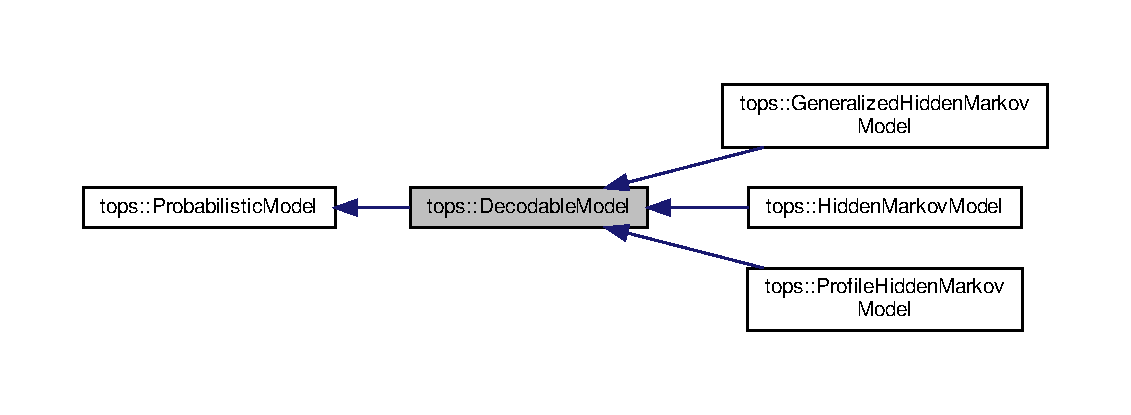
\includegraphics[width=350pt]{classtops_1_1DecodableModel__inherit__graph}
\end{center}
\end{figure}


Collaboration diagram for tops\+:\+:Decodable\+Model\+:
\nopagebreak
\begin{figure}[H]
\begin{center}
\leavevmode
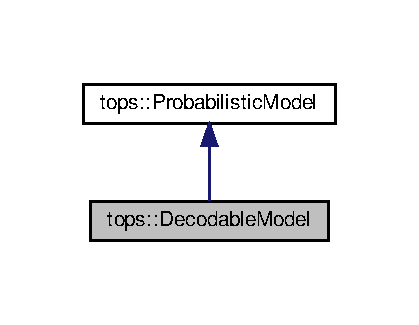
\includegraphics[width=201pt]{classtops_1_1DecodableModel__coll__graph}
\end{center}
\end{figure}
\subsection*{Public Member Functions}
\begin{DoxyCompactItemize}
\item 
\mbox{\Hypertarget{classtops_1_1DecodableModel_aadafde2e7cb86a3d3f261b470e91fbf3}\label{classtops_1_1DecodableModel_aadafde2e7cb86a3d3f261b470e91fbf3}} 
virtual double \hyperlink{classtops_1_1DecodableModel_aadafde2e7cb86a3d3f261b470e91fbf3}{evaluate} (const Sequence \&s, unsigned int begin, unsigned int end) const
\begin{DoxyCompactList}\small\item\em Calculates the sequence likelihood given this model. \end{DoxyCompactList}\item 
\mbox{\Hypertarget{classtops_1_1DecodableModel_a32ae61a80b1ed6f9f5517b0c791b0d0d}\label{classtops_1_1DecodableModel_a32ae61a80b1ed6f9f5517b0c791b0d0d}} 
virtual Sequence \& {\bfseries choose} (Sequence \&h, int \hyperlink{classtops_1_1ProbabilisticModel_a4e3910e9b9b848b7078e7101909ae82a}{size}) const
\item 
\mbox{\Hypertarget{classtops_1_1DecodableModel_a092776d577c0acec332066dcd88e6ee7}\label{classtops_1_1DecodableModel_a092776d577c0acec332066dcd88e6ee7}} 
virtual Sequence \& {\bfseries choose} (Sequence \&h, Sequence \&path, int \hyperlink{classtops_1_1ProbabilisticModel_a4e3910e9b9b848b7078e7101909ae82a}{size}) const
\item 
\mbox{\Hypertarget{classtops_1_1DecodableModel_a7fec7f394ce01a543913cd7414a5dca4}\label{classtops_1_1DecodableModel_a7fec7f394ce01a543913cd7414a5dca4}} 
virtual Sequence \& {\bfseries choose} (Sequence \&h, Sequence \&path, int i, int \hyperlink{classtops_1_1ProbabilisticModel_a4e3910e9b9b848b7078e7101909ae82a}{size}) const
\item 
\mbox{\Hypertarget{classtops_1_1DecodableModel_a607febee2c00a6fd0ac9582def35dbd9}\label{classtops_1_1DecodableModel_a607febee2c00a6fd0ac9582def35dbd9}} 
virtual double \hyperlink{classtops_1_1DecodableModel_a607febee2c00a6fd0ac9582def35dbd9}{forward} (const Sequence \&s, Matrix \&alpha) const =0
\begin{DoxyCompactList}\small\item\em Forward algorithm. \end{DoxyCompactList}\item 
\mbox{\Hypertarget{classtops_1_1DecodableModel_ae2339a90c124e65aabbb9887c04239ff}\label{classtops_1_1DecodableModel_ae2339a90c124e65aabbb9887c04239ff}} 
virtual double \hyperlink{classtops_1_1DecodableModel_ae2339a90c124e65aabbb9887c04239ff}{backward} (const Sequence \&s, Matrix \&beta) const =0
\begin{DoxyCompactList}\small\item\em Backward algorithm. \end{DoxyCompactList}\item 
\mbox{\Hypertarget{classtops_1_1DecodableModel_ab5e3ec33745b4189e8d466895fb51df8}\label{classtops_1_1DecodableModel_ab5e3ec33745b4189e8d466895fb51df8}} 
virtual double \hyperlink{classtops_1_1DecodableModel_ab5e3ec33745b4189e8d466895fb51df8}{viterbi} (const Sequence \&s, Sequence \&path, Matrix \&gamma) const =0
\begin{DoxyCompactList}\small\item\em Viterbi algorithm. \end{DoxyCompactList}\item 
\mbox{\Hypertarget{classtops_1_1DecodableModel_a487a5950464543c60d748fb637f4ed7f}\label{classtops_1_1DecodableModel_a487a5950464543c60d748fb637f4ed7f}} 
virtual void \hyperlink{classtops_1_1DecodableModel_a487a5950464543c60d748fb637f4ed7f}{choose\+Path} (const Sequence \&s, Sequence \&path)
\begin{DoxyCompactList}\small\item\em Choose a path given a sequence. \end{DoxyCompactList}\item 
\mbox{\Hypertarget{classtops_1_1DecodableModel_a5836caa71f5566958086c2fb79b93f22}\label{classtops_1_1DecodableModel_a5836caa71f5566958086c2fb79b93f22}} 
virtual void \hyperlink{classtops_1_1DecodableModel_a5836caa71f5566958086c2fb79b93f22}{posterior\+Probabilities} (const Sequence \&s, Matrix \&probabilities) const
\begin{DoxyCompactList}\small\item\em Posterior Probabilities\+: P(yi=k$\vert$x) \end{DoxyCompactList}\item 
\mbox{\Hypertarget{classtops_1_1DecodableModel_af30ea49ef786a2477e6f8c1311181dd8}\label{classtops_1_1DecodableModel_af30ea49ef786a2477e6f8c1311181dd8}} 
virtual void \hyperlink{classtops_1_1DecodableModel_af30ea49ef786a2477e6f8c1311181dd8}{posterior\+Probabilities} (const Sequence \&s, Sparse\+Matrix\+Ptr probabilities) const
\begin{DoxyCompactList}\small\item\em Posterior Probabilities\+: P(yi=k$\vert$x) \end{DoxyCompactList}\item 
\mbox{\Hypertarget{classtops_1_1DecodableModel_aa11ef25681d465752483d79deb44c0dc}\label{classtops_1_1DecodableModel_aa11ef25681d465752483d79deb44c0dc}} 
virtual void {\bfseries posterior\+Probabilities} (const Sequence \&s, f\+Matrix \&probabilities) const
\item 
\mbox{\Hypertarget{classtops_1_1DecodableModel_a4dc165277061ea987eb994df7fafca6d}\label{classtops_1_1DecodableModel_a4dc165277061ea987eb994df7fafca6d}} 
virtual float {\bfseries M\+E\+A\+Pred} (const Sequence \&s, Sequence \&path)
\item 
\mbox{\Hypertarget{classtops_1_1DecodableModel_a3c2e4577dda5374cac0287e0fc1ec04f}\label{classtops_1_1DecodableModel_a3c2e4577dda5374cac0287e0fc1ec04f}} 
virtual float {\bfseries M\+E\+A\+Pred} (const Sequence \&s, Sequence \&path, Sparse\+Matrix\+Ptr post\+Probs)
\item 
\mbox{\Hypertarget{classtops_1_1DecodableModel_a0e243fa34e02349602faae53cae86a41}\label{classtops_1_1DecodableModel_a0e243fa34e02349602faae53cae86a41}} 
virtual void \hyperlink{classtops_1_1DecodableModel_a0e243fa34e02349602faae53cae86a41}{posterior\+Decoding} (const Sequence \&s, Sequence \&path, Matrix \&probabilities) const
\begin{DoxyCompactList}\small\item\em Posterior Decoding\+: $^\wedge$yi = argmax\+\_\+k P(yi=k$\vert$x) \end{DoxyCompactList}\item 
virtual Sequence \& \hyperlink{classtops_1_1DecodableModel_a9321fd7bca21551b4c5380e1f48ff5c2}{choose\+Observation} (Sequence \&h, int i, int state) const =0
\begin{DoxyCompactList}\small\item\em Choose the observation given a state. \end{DoxyCompactList}\item 
\mbox{\Hypertarget{classtops_1_1DecodableModel_a7bac54cfa355803764cf8677d58cbe70}\label{classtops_1_1DecodableModel_a7bac54cfa355803764cf8677d58cbe70}} 
virtual int \hyperlink{classtops_1_1DecodableModel_a7bac54cfa355803764cf8677d58cbe70}{choose\+State} (int state) const =0
\begin{DoxyCompactList}\small\item\em Choose a state. \end{DoxyCompactList}\item 
\mbox{\Hypertarget{classtops_1_1DecodableModel_ac31959a6d852e2e00938294bd54f2667}\label{classtops_1_1DecodableModel_ac31959a6d852e2e00938294bd54f2667}} 
virtual int \hyperlink{classtops_1_1DecodableModel_ac31959a6d852e2e00938294bd54f2667}{choose\+First\+State} () const =0
\begin{DoxyCompactList}\small\item\em Choose the initial state. \end{DoxyCompactList}\item 
\mbox{\Hypertarget{classtops_1_1DecodableModel_aee6d21ab65252b50d335358b05a1aee9}\label{classtops_1_1DecodableModel_aee6d21ab65252b50d335358b05a1aee9}} 
virtual std\+::string \hyperlink{classtops_1_1DecodableModel_aee6d21ab65252b50d335358b05a1aee9}{get\+State\+Name} (int state) const =0
\begin{DoxyCompactList}\small\item\em Get state name. \end{DoxyCompactList}\item 
\mbox{\Hypertarget{classtops_1_1DecodableModel_aba6a89196c2cb2349349166227fc1e8b}\label{classtops_1_1DecodableModel_aba6a89196c2cb2349349166227fc1e8b}} 
virtual Alphabet\+Ptr \hyperlink{classtops_1_1DecodableModel_aba6a89196c2cb2349349166227fc1e8b}{get\+State\+Names} () const =0
\begin{DoxyCompactList}\small\item\em Get the state names. \end{DoxyCompactList}\item 
\mbox{\Hypertarget{classtops_1_1DecodableModel_a37326b129c2a20b12c79c1b2488adc93}\label{classtops_1_1DecodableModel_a37326b129c2a20b12c79c1b2488adc93}} 
virtual \hyperlink{classtops_1_1DecodableModel}{Decodable\+Model} $\ast$ {\bfseries decodable} ()
\end{DoxyCompactItemize}


\subsection{Detailed Description}
Interface defining probabilistic model with the viterbi, forward and backward algorithm. 

Definition at line 38 of file Decodable\+Model.\+hpp.



\subsection{Member Function Documentation}
\mbox{\Hypertarget{classtops_1_1DecodableModel_a9321fd7bca21551b4c5380e1f48ff5c2}\label{classtops_1_1DecodableModel_a9321fd7bca21551b4c5380e1f48ff5c2}} 
\index{tops\+::\+Decodable\+Model@{tops\+::\+Decodable\+Model}!choose\+Observation@{choose\+Observation}}
\index{choose\+Observation@{choose\+Observation}!tops\+::\+Decodable\+Model@{tops\+::\+Decodable\+Model}}
\subsubsection{\texorpdfstring{choose\+Observation()}{chooseObservation()}}
{\footnotesize\ttfamily virtual Sequence\& tops\+::\+Decodable\+Model\+::choose\+Observation (\begin{DoxyParamCaption}\item[{Sequence \&}]{h,  }\item[{int}]{i,  }\item[{int}]{state }\end{DoxyParamCaption}) const\hspace{0.3cm}{\ttfamily [pure virtual]}}



Choose the observation given a state. 


\begin{DoxyParams}{Parameters}
{\em h} & is the history \\
\hline
\end{DoxyParams}


Implemented in \hyperlink{classtops_1_1GeneralizedHiddenMarkovModel_a233bb11a876558c449713e274f0f7f6c}{tops\+::\+Generalized\+Hidden\+Markov\+Model}, \hyperlink{classtops_1_1HiddenMarkovModel_af9085a6ee9df355a207b0090d2eae284}{tops\+::\+Hidden\+Markov\+Model}, and \hyperlink{classtops_1_1ProfileHiddenMarkovModel_a369bbe95930890c2460ee1b56b4415f5}{tops\+::\+Profile\+Hidden\+Markov\+Model}.



The documentation for this class was generated from the following files\+:\begin{DoxyCompactItemize}
\item 
src/Decodable\+Model.\+hpp\item 
src/Decodable\+Model.\+cpp\end{DoxyCompactItemize}

\hypertarget{classtops_1_1DegenerateDistribution}{}\section{tops\+:\+:Degenerate\+Distribution Class Reference}
\label{classtops_1_1DegenerateDistribution}\index{tops\+::\+Degenerate\+Distribution@{tops\+::\+Degenerate\+Distribution}}


A probabilistic model that emits a constant integer value.  




{\ttfamily \#include $<$Degenerate\+Distribution.\+hpp$>$}



Inheritance diagram for tops\+:\+:Degenerate\+Distribution\+:
\nopagebreak
\begin{figure}[H]
\begin{center}
\leavevmode
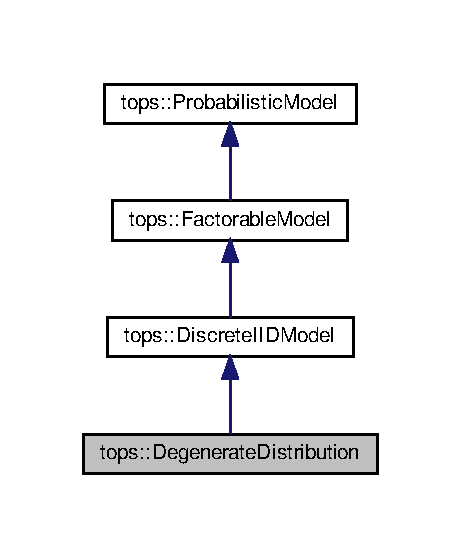
\includegraphics[width=221pt]{classtops_1_1DegenerateDistribution__inherit__graph}
\end{center}
\end{figure}


Collaboration diagram for tops\+:\+:Degenerate\+Distribution\+:
\nopagebreak
\begin{figure}[H]
\begin{center}
\leavevmode
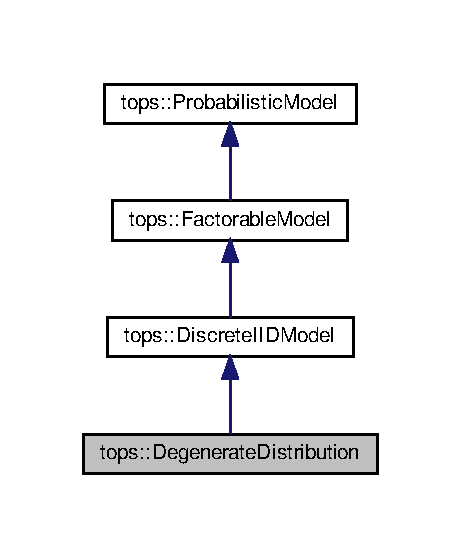
\includegraphics[width=221pt]{classtops_1_1DegenerateDistribution__coll__graph}
\end{center}
\end{figure}
\subsection*{Public Member Functions}
\begin{DoxyCompactItemize}
\item 
\mbox{\Hypertarget{classtops_1_1DegenerateDistribution_aab108d57cf25544ae2afd68939c69329}\label{classtops_1_1DegenerateDistribution_aab108d57cf25544ae2afd68939c69329}} 
{\bfseries Degenerate\+Distribution} (int c)
\item 
\mbox{\Hypertarget{classtops_1_1DegenerateDistribution_a08aef108f6ede16a15ebeac9e81afbde}\label{classtops_1_1DegenerateDistribution_a08aef108f6ede16a15ebeac9e81afbde}} 
virtual double \hyperlink{classtops_1_1DegenerateDistribution_a08aef108f6ede16a15ebeac9e81afbde}{evaluate} (const Sequence \&sequence, unsigned int begin, unsigned int end) const
\begin{DoxyCompactList}\small\item\em Calculates the sequence likelihood given the model. \end{DoxyCompactList}\item 
\mbox{\Hypertarget{classtops_1_1DegenerateDistribution_aefd0aff98e9b81510550688038d0f9dc}\label{classtops_1_1DegenerateDistribution_aefd0aff98e9b81510550688038d0f9dc}} 
virtual double \hyperlink{classtops_1_1DegenerateDistribution_aefd0aff98e9b81510550688038d0f9dc}{choose} (Sequence \&s, unsigned int \hyperlink{classtops_1_1DiscreteIIDModel_aa486a4a7ba0b77de10160eddce2c8ef5}{size}) const
\begin{DoxyCompactList}\small\item\em Generates a sequence by the simulation of the model. \end{DoxyCompactList}\item 
\mbox{\Hypertarget{classtops_1_1DegenerateDistribution_a04c33d3d4992195d27bb6a087b1f487a}\label{classtops_1_1DegenerateDistribution_a04c33d3d4992195d27bb6a087b1f487a}} 
virtual std\+::string \hyperlink{classtops_1_1DegenerateDistribution_a04c33d3d4992195d27bb6a087b1f487a}{str} () const
\begin{DoxyCompactList}\small\item\em returns the string representation of the model \end{DoxyCompactList}\item 
\mbox{\Hypertarget{classtops_1_1DegenerateDistribution_acec7ad29c607ac20f230569324275847}\label{classtops_1_1DegenerateDistribution_acec7ad29c607ac20f230569324275847}} 
virtual double \& {\bfseries log\+\_\+probability\+\_\+of} (int c)
\item 
\mbox{\Hypertarget{classtops_1_1DegenerateDistribution_a86f4898dc1294c4ee80d183403b4a686}\label{classtops_1_1DegenerateDistribution_a86f4898dc1294c4ee80d183403b4a686}} 
virtual int \hyperlink{classtops_1_1DegenerateDistribution_a86f4898dc1294c4ee80d183403b4a686}{choose} () const
\begin{DoxyCompactList}\small\item\em Choose. \end{DoxyCompactList}\end{DoxyCompactItemize}
\subsection*{Friends}
\begin{DoxyCompactItemize}
\item 
\mbox{\Hypertarget{classtops_1_1DegenerateDistribution_ac98d07dd8f7b70e16ccb9a01abf56b9c}\label{classtops_1_1DegenerateDistribution_ac98d07dd8f7b70e16ccb9a01abf56b9c}} 
class {\bfseries boost\+::serialization\+::access}
\end{DoxyCompactItemize}


\subsection{Detailed Description}
A probabilistic model that emits a constant integer value. 

Definition at line 34 of file Degenerate\+Distribution.\+hpp.



The documentation for this class was generated from the following file\+:\begin{DoxyCompactItemize}
\item 
src/Degenerate\+Distribution.\+hpp\end{DoxyCompactItemize}

\hypertarget{classtops_1_1DiscreteIIDModel}{}\section{tops\+:\+:Discrete\+I\+I\+D\+Model Class Reference}
\label{classtops_1_1DiscreteIIDModel}\index{tops\+::\+Discrete\+I\+I\+D\+Model@{tops\+::\+Discrete\+I\+I\+D\+Model}}


This represent probability distributions over a finite set of symbols.  




{\ttfamily \#include $<$Discrete\+I\+I\+D\+Model.\+hpp$>$}



Inheritance diagram for tops\+:\+:Discrete\+I\+I\+D\+Model\+:
\nopagebreak
\begin{figure}[H]
\begin{center}
\leavevmode
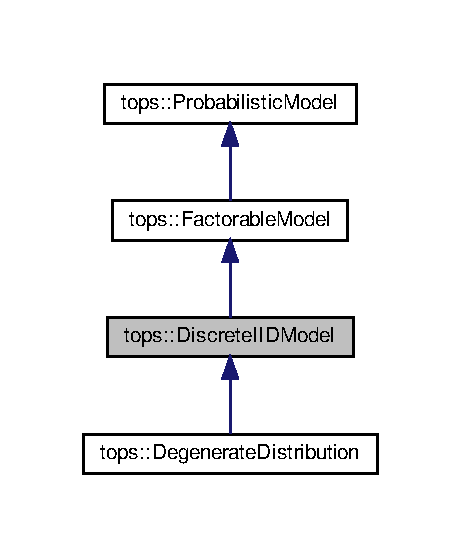
\includegraphics[width=221pt]{classtops_1_1DiscreteIIDModel__inherit__graph}
\end{center}
\end{figure}


Collaboration diagram for tops\+:\+:Discrete\+I\+I\+D\+Model\+:
\nopagebreak
\begin{figure}[H]
\begin{center}
\leavevmode
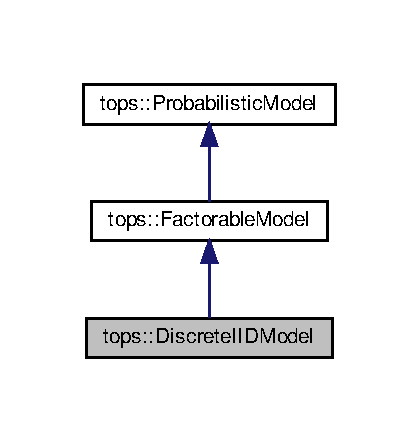
\includegraphics[width=201pt]{classtops_1_1DiscreteIIDModel__coll__graph}
\end{center}
\end{figure}
\subsection*{Public Member Functions}
\begin{DoxyCompactItemize}
\item 
\hyperlink{classtops_1_1DiscreteIIDModel_a229cd565d9c721d9524f3aff2a5a4532}{Discrete\+I\+I\+D\+Model} (const Double\+Vector \&probabilities)
\begin{DoxyCompactList}\small\item\em Constructor. \end{DoxyCompactList}\item 
\mbox{\Hypertarget{classtops_1_1DiscreteIIDModel_a76f0b01fc969d306ea3a4165023e2941}\label{classtops_1_1DiscreteIIDModel_a76f0b01fc969d306ea3a4165023e2941}} 
{\bfseries Discrete\+I\+I\+D\+Model} (const Matrix \&probabilities)
\item 
\mbox{\Hypertarget{classtops_1_1DiscreteIIDModel_a71d8b5b349b073b831fb8a02a6a963b9}\label{classtops_1_1DiscreteIIDModel_a71d8b5b349b073b831fb8a02a6a963b9}} 
virtual double \hyperlink{classtops_1_1DiscreteIIDModel_a71d8b5b349b073b831fb8a02a6a963b9}{choose} () const
\begin{DoxyCompactList}\small\item\em Choose. \end{DoxyCompactList}\item 
\mbox{\Hypertarget{classtops_1_1DiscreteIIDModel_a944742bf86b64299af198f54c3f5affb}\label{classtops_1_1DiscreteIIDModel_a944742bf86b64299af198f54c3f5affb}} 
virtual void {\bfseries choose\+Pair} (int $\ast$a, int $\ast$b) const
\item 
\mbox{\Hypertarget{classtops_1_1DiscreteIIDModel_a1d932c0abddc9a93430fee7a0e3bd990}\label{classtops_1_1DiscreteIIDModel_a1d932c0abddc9a93430fee7a0e3bd990}} 
virtual double \hyperlink{classtops_1_1DiscreteIIDModel_a1d932c0abddc9a93430fee7a0e3bd990}{log\+\_\+probability\+\_\+of} (int s) const
\begin{DoxyCompactList}\small\item\em Returns the log\+\_\+probability\+\_\+of the number s. \end{DoxyCompactList}\item 
\mbox{\Hypertarget{classtops_1_1DiscreteIIDModel_a4a4dbdd358d8823892da0a8039c5489a}\label{classtops_1_1DiscreteIIDModel_a4a4dbdd358d8823892da0a8039c5489a}} 
virtual double {\bfseries log\+\_\+probability\+\_\+of\+\_\+pair} (int s1, int s2) const
\item 
\mbox{\Hypertarget{classtops_1_1DiscreteIIDModel_a6792ac1608ed7841b46bf8a4a034e8fe}\label{classtops_1_1DiscreteIIDModel_a6792ac1608ed7841b46bf8a4a034e8fe}} 
void {\bfseries str\+Matrix} () const
\item 
\mbox{\Hypertarget{classtops_1_1DiscreteIIDModel_ab1d33f6f6da4a3c655d7356887635d26}\label{classtops_1_1DiscreteIIDModel_ab1d33f6f6da4a3c655d7356887635d26}} 
virtual double \hyperlink{classtops_1_1DiscreteIIDModel_ab1d33f6f6da4a3c655d7356887635d26}{log\+\_\+probability\+\_\+of} (int s, double new\+\_\+value)
\begin{DoxyCompactList}\small\item\em Set the probability value of the number s. \end{DoxyCompactList}\item 
\mbox{\Hypertarget{classtops_1_1DiscreteIIDModel_a4e556ccbe56950a4d7dd3fb8aaaff19b}\label{classtops_1_1DiscreteIIDModel_a4e556ccbe56950a4d7dd3fb8aaaff19b}} 
virtual double \hyperlink{classtops_1_1DiscreteIIDModel_a4e556ccbe56950a4d7dd3fb8aaaff19b}{evaluate\+Position} (const Sequence \&s, unsigned int i) const
\begin{DoxyCompactList}\small\item\em Evaluate the position i of the sequence s. \end{DoxyCompactList}\item 
\mbox{\Hypertarget{classtops_1_1DiscreteIIDModel_abdf5a2ac3291dd78e81bd44d1366ee41}\label{classtops_1_1DiscreteIIDModel_abdf5a2ac3291dd78e81bd44d1366ee41}} 
virtual double {\bfseries log\+\_\+probability\+\_\+of\+\_\+pair} (int s1, int s2, double new\+\_\+value)
\item 
\mbox{\Hypertarget{classtops_1_1DiscreteIIDModel_a2dbe94da17ac80a986a356de7145872b}\label{classtops_1_1DiscreteIIDModel_a2dbe94da17ac80a986a356de7145872b}} 
virtual double \hyperlink{classtops_1_1DiscreteIIDModel_a2dbe94da17ac80a986a356de7145872b}{choose\+Position} (const Sequence \&s, int i) const
\begin{DoxyCompactList}\small\item\em Choose the position i of the sequence s given the subsequence before the position i. \end{DoxyCompactList}\item 
\mbox{\Hypertarget{classtops_1_1DiscreteIIDModel_a8ae9284850a6277e1eb893dd3fd03498}\label{classtops_1_1DiscreteIIDModel_a8ae9284850a6277e1eb893dd3fd03498}} 
virtual std\+::string \hyperlink{classtops_1_1DiscreteIIDModel_a8ae9284850a6277e1eb893dd3fd03498}{model\+\_\+name} () const
\begin{DoxyCompactList}\small\item\em returns the model name \end{DoxyCompactList}\item 
\mbox{\Hypertarget{classtops_1_1DiscreteIIDModel_a62218b116d392f5d64a373d94fb79bbc}\label{classtops_1_1DiscreteIIDModel_a62218b116d392f5d64a373d94fb79bbc}} 
virtual Probabilistic\+Model\+Creator\+Ptr {\bfseries get\+Factory} () const
\item 
\mbox{\Hypertarget{classtops_1_1DiscreteIIDModel_aa486a4a7ba0b77de10160eddce2c8ef5}\label{classtops_1_1DiscreteIIDModel_aa486a4a7ba0b77de10160eddce2c8ef5}} 
virtual int \hyperlink{classtops_1_1DiscreteIIDModel_aa486a4a7ba0b77de10160eddce2c8ef5}{size} () const
\begin{DoxyCompactList}\small\item\em Returns the number of parameters of the model. \end{DoxyCompactList}\item 
\mbox{\Hypertarget{classtops_1_1DiscreteIIDModel_a789bb1abb116d6d2129b7d2316a9078e}\label{classtops_1_1DiscreteIIDModel_a789bb1abb116d6d2129b7d2316a9078e}} 
virtual std\+::string \hyperlink{classtops_1_1DiscreteIIDModel_a789bb1abb116d6d2129b7d2316a9078e}{str} () const
\begin{DoxyCompactList}\small\item\em returns the string representation of the model \end{DoxyCompactList}\item 
\mbox{\Hypertarget{classtops_1_1DiscreteIIDModel_ae13af8f2d01b6c80c2966dec700ebb36}\label{classtops_1_1DiscreteIIDModel_ae13af8f2d01b6c80c2966dec700ebb36}} 
virtual void {\bfseries initialize\+From\+Map} (const std\+::map$<$ std\+::string, double $>$ \&probabilities, Alphabet\+Ptr \hyperlink{classtops_1_1ProbabilisticModel_acacbfeb9cce968e034b5c18c72f7e217}{alphabet})
\item 
\mbox{\Hypertarget{classtops_1_1DiscreteIIDModel_a7304a326d3a637434709648a29226c0e}\label{classtops_1_1DiscreteIIDModel_a7304a326d3a637434709648a29226c0e}} 
virtual void {\bfseries initialize} (const \hyperlink{classtops_1_1ProbabilisticModelParameters}{Probabilistic\+Model\+Parameters} \&p)
\item 
\mbox{\Hypertarget{classtops_1_1DiscreteIIDModel_aa144ea7f69b42517343170dd44cf50e8}\label{classtops_1_1DiscreteIIDModel_aa144ea7f69b42517343170dd44cf50e8}} 
virtual \hyperlink{classtops_1_1ProbabilisticModelParameters}{Probabilistic\+Model\+Parameters} {\bfseries parameters} () const
\item 
\mbox{\Hypertarget{classtops_1_1DiscreteIIDModel_a607a50d8fca66f3f71970830cc08c728}\label{classtops_1_1DiscreteIIDModel_a607a50d8fca66f3f71970830cc08c728}} 
void {\bfseries set\+Probabilities} (const Double\+Vector \&probabilities)
\end{DoxyCompactItemize}


\subsection{Detailed Description}
This represent probability distributions over a finite set of symbols. 

Definition at line 42 of file Discrete\+I\+I\+D\+Model.\+hpp.



\subsection{Constructor \& Destructor Documentation}
\mbox{\Hypertarget{classtops_1_1DiscreteIIDModel_a229cd565d9c721d9524f3aff2a5a4532}\label{classtops_1_1DiscreteIIDModel_a229cd565d9c721d9524f3aff2a5a4532}} 
\index{tops\+::\+Discrete\+I\+I\+D\+Model@{tops\+::\+Discrete\+I\+I\+D\+Model}!Discrete\+I\+I\+D\+Model@{Discrete\+I\+I\+D\+Model}}
\index{Discrete\+I\+I\+D\+Model@{Discrete\+I\+I\+D\+Model}!tops\+::\+Discrete\+I\+I\+D\+Model@{tops\+::\+Discrete\+I\+I\+D\+Model}}
\subsubsection{\texorpdfstring{Discrete\+I\+I\+D\+Model()}{DiscreteIIDModel()}}
{\footnotesize\ttfamily tops\+::\+Discrete\+I\+I\+D\+Model\+::\+Discrete\+I\+I\+D\+Model (\begin{DoxyParamCaption}\item[{const Double\+Vector \&}]{probabilities }\end{DoxyParamCaption})}



Constructor. 


\begin{DoxyParams}{Parameters}
{\em probabilities} & is the probabilities value \\
\hline
\end{DoxyParams}


Definition at line 36 of file Discrete\+I\+I\+D\+Model.\+cpp.


\begin{DoxyCode}
37   \{
38     \_size = probabilities.size() - 1;
39     \_log\_probabilities.resize(\_size+1);
40     \textcolor{keywordtype}{double}  sum = 0;
41     \textcolor{keywordflow}{for}(\textcolor{keywordtype}{unsigned} \textcolor{keywordtype}{int} i = 0; i < probabilities.size(); i++)
42       sum += probabilities[i];
43     \textcolor{keywordflow}{for}(\textcolor{keywordtype}{int} i = 0; (i <= \_size); i++)
44       \textcolor{keywordflow}{if}(i >= (\textcolor{keywordtype}{int})probabilities.size())
45         \_log\_probabilities[i] = -HUGE;
46       \textcolor{keywordflow}{else} \textcolor{keywordflow}{if}(close(probabilities[i], 0.0, 1e-10))
47         \_log\_probabilities[i] = -HUGE;
48       \textcolor{keywordflow}{else}
49         \_log\_probabilities[i] = log(probabilities[i]/sum);
50      \_geometric\_tail = \textcolor{keyword}{false};
51   \}
\end{DoxyCode}


The documentation for this class was generated from the following files\+:\begin{DoxyCompactItemize}
\item 
src/Discrete\+I\+I\+D\+Model.\+hpp\item 
src/Discrete\+I\+I\+D\+Model.\+cpp\end{DoxyCompactItemize}

\hypertarget{classtops_1_1DiscreteIIDModelCreator}{}\section{tops\+:\+:Discrete\+I\+I\+D\+Model\+Creator Class Reference}
\label{classtops_1_1DiscreteIIDModelCreator}\index{tops\+::\+Discrete\+I\+I\+D\+Model\+Creator@{tops\+::\+Discrete\+I\+I\+D\+Model\+Creator}}


This class is a factory for the finite discrete distribution.  




{\ttfamily \#include $<$Discrete\+I\+I\+D\+Model\+Creator.\+hpp$>$}



Inheritance diagram for tops\+:\+:Discrete\+I\+I\+D\+Model\+Creator\+:
\nopagebreak
\begin{figure}[H]
\begin{center}
\leavevmode
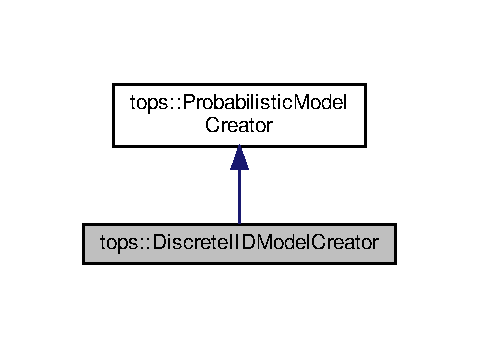
\includegraphics[width=230pt]{classtops_1_1DiscreteIIDModelCreator__inherit__graph}
\end{center}
\end{figure}


Collaboration diagram for tops\+:\+:Discrete\+I\+I\+D\+Model\+Creator\+:
\nopagebreak
\begin{figure}[H]
\begin{center}
\leavevmode
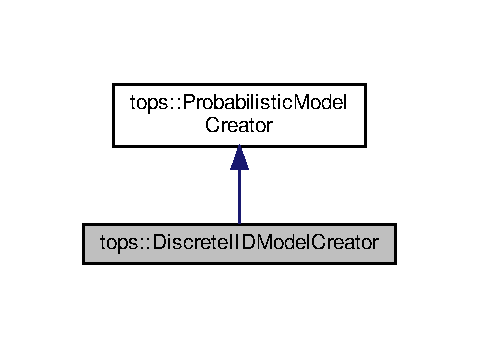
\includegraphics[width=230pt]{classtops_1_1DiscreteIIDModelCreator__coll__graph}
\end{center}
\end{figure}
\subsection*{Public Member Functions}
\begin{DoxyCompactItemize}
\item 
virtual Probabilistic\+Model\+Ptr \hyperlink{classtops_1_1DiscreteIIDModelCreator_a3eeca79afe4c57388385fed4299421d6}{create} (\hyperlink{classtops_1_1ProbabilisticModelParameters}{Probabilistic\+Model\+Parameters} \&parameters) const
\begin{DoxyCompactList}\small\item\em Creates a probabilistic model. \end{DoxyCompactList}\item 
\mbox{\Hypertarget{classtops_1_1DiscreteIIDModelCreator_a192c687e49763a08045f9c2d6728a6ed}\label{classtops_1_1DiscreteIIDModelCreator_a192c687e49763a08045f9c2d6728a6ed}} 
virtual Discrete\+I\+I\+D\+Model\+Ptr {\bfseries create\+Discrete\+I\+I\+D\+Model} (\hyperlink{classtops_1_1ProbabilisticModelParameters}{Probabilistic\+Model\+Parameters} \&parameters) const
\item 
\mbox{\Hypertarget{classtops_1_1DiscreteIIDModelCreator_afc22fa730452ff88495f66341ffbfb34}\label{classtops_1_1DiscreteIIDModelCreator_afc22fa730452ff88495f66341ffbfb34}} 
virtual std\+::string \hyperlink{classtops_1_1DiscreteIIDModelCreator_afc22fa730452ff88495f66341ffbfb34}{help} () const
\begin{DoxyCompactList}\small\item\em This method returns a help message. \end{DoxyCompactList}\end{DoxyCompactItemize}


\subsection{Detailed Description}
This class is a factory for the finite discrete distribution. 

Definition at line 37 of file Discrete\+I\+I\+D\+Model\+Creator.\+hpp.



\subsection{Member Function Documentation}
\mbox{\Hypertarget{classtops_1_1DiscreteIIDModelCreator_a3eeca79afe4c57388385fed4299421d6}\label{classtops_1_1DiscreteIIDModelCreator_a3eeca79afe4c57388385fed4299421d6}} 
\index{tops\+::\+Discrete\+I\+I\+D\+Model\+Creator@{tops\+::\+Discrete\+I\+I\+D\+Model\+Creator}!create@{create}}
\index{create@{create}!tops\+::\+Discrete\+I\+I\+D\+Model\+Creator@{tops\+::\+Discrete\+I\+I\+D\+Model\+Creator}}
\subsubsection{\texorpdfstring{create()}{create()}}
{\footnotesize\ttfamily Probabilistic\+Model\+Ptr tops\+::\+Discrete\+I\+I\+D\+Model\+Creator\+::create (\begin{DoxyParamCaption}\item[{\hyperlink{classtops_1_1ProbabilisticModelParameters}{Probabilistic\+Model\+Parameters} \&}]{parameters }\end{DoxyParamCaption}) const\hspace{0.3cm}{\ttfamily [virtual]}}



Creates a probabilistic model. 


\begin{DoxyParams}{Parameters}
{\em parameters} & is a set of parameters that is utilized to build the model \\
\hline
\end{DoxyParams}


Reimplemented from \hyperlink{classtops_1_1ProbabilisticModelCreator_afed6c8ffa45fff446bdaa8b533da8f7c}{tops\+::\+Probabilistic\+Model\+Creator}.



Definition at line 31 of file Discrete\+I\+I\+D\+Model\+Creator.\+cpp.


\begin{DoxyCode}
31                                                                                                        \{
32     \textcolor{keywordflow}{return} createDiscreteIIDModel(parameters);
33   \}
\end{DoxyCode}


The documentation for this class was generated from the following files\+:\begin{DoxyCompactItemize}
\item 
src/Discrete\+I\+I\+D\+Model\+Creator.\+hpp\item 
src/Discrete\+I\+I\+D\+Model\+Creator.\+cpp\end{DoxyCompactItemize}

\hypertarget{classtops_1_1DoubleListParameterValue2}{}\section{tops\+:\+:Double\+List\+Parameter\+Value2 Class Reference}
\label{classtops_1_1DoubleListParameterValue2}\index{tops\+::\+Double\+List\+Parameter\+Value2@{tops\+::\+Double\+List\+Parameter\+Value2}}


Inheritance diagram for tops\+:\+:Double\+List\+Parameter\+Value2\+:
\nopagebreak
\begin{figure}[H]
\begin{center}
\leavevmode
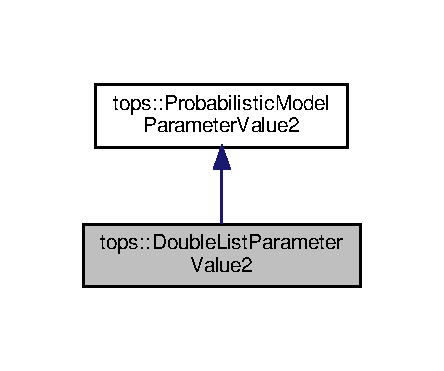
\includegraphics[width=213pt]{classtops_1_1DoubleListParameterValue2__inherit__graph}
\end{center}
\end{figure}


Collaboration diagram for tops\+:\+:Double\+List\+Parameter\+Value2\+:
\nopagebreak
\begin{figure}[H]
\begin{center}
\leavevmode
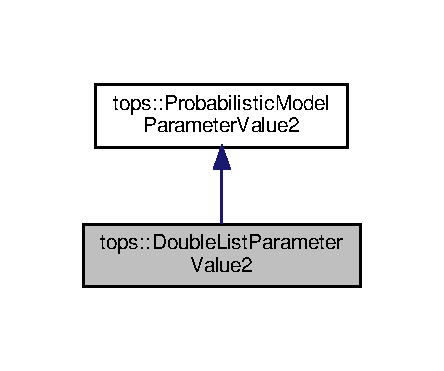
\includegraphics[width=213pt]{classtops_1_1DoubleListParameterValue2__coll__graph}
\end{center}
\end{figure}
\subsection*{Public Member Functions}
\begin{DoxyCompactItemize}
\item 
\mbox{\Hypertarget{classtops_1_1DoubleListParameterValue2_aba397c523171e51c31500540f5dea809}\label{classtops_1_1DoubleListParameterValue2_aba397c523171e51c31500540f5dea809}} 
{\bfseries Double\+List\+Parameter\+Value2} (std\+::vector$<$ double $>$ value)
\item 
\mbox{\Hypertarget{classtops_1_1DoubleListParameterValue2_a9eadec4e5c307d58f7b991ca69e4f2b0}\label{classtops_1_1DoubleListParameterValue2_a9eadec4e5c307d58f7b991ca69e4f2b0}} 
std\+::vector$<$ double $>$ {\bfseries value} ()
\item 
\mbox{\Hypertarget{classtops_1_1DoubleListParameterValue2_a3ffe1b1b4c3860ce33fec98cd25630df}\label{classtops_1_1DoubleListParameterValue2_a3ffe1b1b4c3860ce33fec98cd25630df}} 
virtual std\+::string {\bfseries parameter\+Type} ()
\item 
\mbox{\Hypertarget{classtops_1_1DoubleListParameterValue2_a0dffa07dc65126e7e4de9d9ae09e43d8}\label{classtops_1_1DoubleListParameterValue2_a0dffa07dc65126e7e4de9d9ae09e43d8}} 
virtual std\+::string {\bfseries str} ()
\end{DoxyCompactItemize}


\subsection{Detailed Description}


Definition at line 88 of file Probabilistic\+Model\+Parameter\+Value2.\+hpp.



The documentation for this class was generated from the following files\+:\begin{DoxyCompactItemize}
\item 
src/Probabilistic\+Model\+Parameter\+Value2.\+hpp\item 
src/Probabilistic\+Model\+Parameter\+Value2.\+cpp\end{DoxyCompactItemize}

\hypertarget{classtops_1_1DoubleMapParameterValue}{}\section{tops\+:\+:Double\+Map\+Parameter\+Value Class Reference}
\label{classtops_1_1DoubleMapParameterValue}\index{tops\+::\+Double\+Map\+Parameter\+Value@{tops\+::\+Double\+Map\+Parameter\+Value}}


probability table  




{\ttfamily \#include $<$Probabilistic\+Model\+Parameter.\+hpp$>$}



Inheritance diagram for tops\+:\+:Double\+Map\+Parameter\+Value\+:
\nopagebreak
\begin{figure}[H]
\begin{center}
\leavevmode
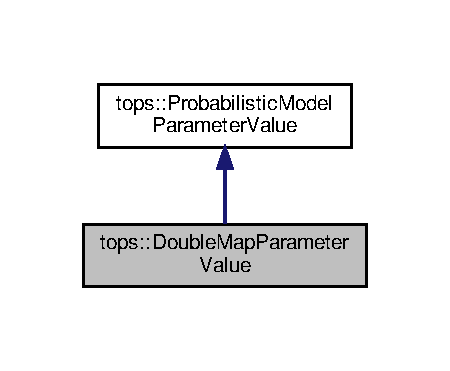
\includegraphics[width=216pt]{classtops_1_1DoubleMapParameterValue__inherit__graph}
\end{center}
\end{figure}


Collaboration diagram for tops\+:\+:Double\+Map\+Parameter\+Value\+:
\nopagebreak
\begin{figure}[H]
\begin{center}
\leavevmode
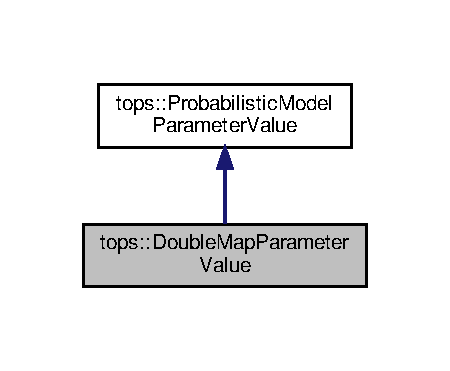
\includegraphics[width=216pt]{classtops_1_1DoubleMapParameterValue__coll__graph}
\end{center}
\end{figure}
\subsection*{Public Member Functions}
\begin{DoxyCompactItemize}
\item 
\mbox{\Hypertarget{classtops_1_1DoubleMapParameterValue_aa2fd10d6c30872eeb61f0dc947c532a0}\label{classtops_1_1DoubleMapParameterValue_aa2fd10d6c30872eeb61f0dc947c532a0}} 
{\bfseries Double\+Map\+Parameter\+Value} (const std\+::map$<$ std\+::string, double $>$ \&values)
\item 
\mbox{\Hypertarget{classtops_1_1DoubleMapParameterValue_aa6b87b6f8903190e67d1b0de0119c6c9}\label{classtops_1_1DoubleMapParameterValue_aa6b87b6f8903190e67d1b0de0119c6c9}} 
virtual void {\bfseries initialize} (const std\+::map$<$ std\+::string, double $>$ \&values)
\item 
\mbox{\Hypertarget{classtops_1_1DoubleMapParameterValue_a75e63c08b1ff511654ad5ecdc77e37f1}\label{classtops_1_1DoubleMapParameterValue_a75e63c08b1ff511654ad5ecdc77e37f1}} 
virtual std\+::string {\bfseries parameter\+\_\+type} () const
\item 
\mbox{\Hypertarget{classtops_1_1DoubleMapParameterValue_a2a5509470f922714c774dce7776b70aa}\label{classtops_1_1DoubleMapParameterValue_a2a5509470f922714c774dce7776b70aa}} 
{\bfseries Double\+Map\+Parameter\+Value} (std\+::vector$<$ std\+::string $>$ keys, std\+::vector$<$ double $>$ value)
\item 
\mbox{\Hypertarget{classtops_1_1DoubleMapParameterValue_a214ef931cd0400b0be92feeed773acf9}\label{classtops_1_1DoubleMapParameterValue_a214ef931cd0400b0be92feeed773acf9}} 
virtual std\+::map$<$ std\+::string, double $>$ \& {\bfseries get\+Double\+Map} ()
\item 
\mbox{\Hypertarget{classtops_1_1DoubleMapParameterValue_a25f2d12177f6c5bbcb5fb42b118bcdbd}\label{classtops_1_1DoubleMapParameterValue_a25f2d12177f6c5bbcb5fb42b118bcdbd}} 
virtual std\+::string {\bfseries str} () const
\end{DoxyCompactItemize}


\subsection{Detailed Description}
probability table 

Definition at line 183 of file Probabilistic\+Model\+Parameter.\+hpp.



The documentation for this class was generated from the following files\+:\begin{DoxyCompactItemize}
\item 
src/Probabilistic\+Model\+Parameter.\+hpp\item 
src/Probabilistic\+Model\+Parameter.\+cpp\end{DoxyCompactItemize}

\hypertarget{classtops_1_1DoubleParameterValue}{}\section{tops\+:\+:Double\+Parameter\+Value Class Reference}
\label{classtops_1_1DoubleParameterValue}\index{tops\+::\+Double\+Parameter\+Value@{tops\+::\+Double\+Parameter\+Value}}


Double parameter value.  




{\ttfamily \#include $<$Probabilistic\+Model\+Parameter.\+hpp$>$}



Inheritance diagram for tops\+:\+:Double\+Parameter\+Value\+:
\nopagebreak
\begin{figure}[H]
\begin{center}
\leavevmode
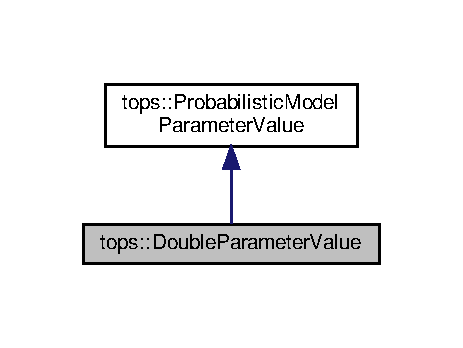
\includegraphics[width=222pt]{classtops_1_1DoubleParameterValue__inherit__graph}
\end{center}
\end{figure}


Collaboration diagram for tops\+:\+:Double\+Parameter\+Value\+:
\nopagebreak
\begin{figure}[H]
\begin{center}
\leavevmode
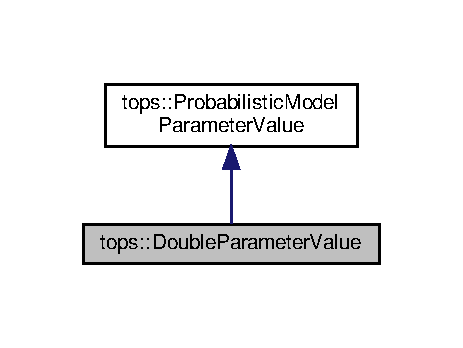
\includegraphics[width=222pt]{classtops_1_1DoubleParameterValue__coll__graph}
\end{center}
\end{figure}
\subsection*{Public Member Functions}
\begin{DoxyCompactItemize}
\item 
\mbox{\Hypertarget{classtops_1_1DoubleParameterValue_ad5fc3759fdf4b74e261685c97f3cd00f}\label{classtops_1_1DoubleParameterValue_ad5fc3759fdf4b74e261685c97f3cd00f}} 
virtual void {\bfseries initialize} (double d)
\item 
\mbox{\Hypertarget{classtops_1_1DoubleParameterValue_a9145ee3c39138c923d5b8c02ade984e4}\label{classtops_1_1DoubleParameterValue_a9145ee3c39138c923d5b8c02ade984e4}} 
{\bfseries Double\+Parameter\+Value} (double d)
\item 
\mbox{\Hypertarget{classtops_1_1DoubleParameterValue_a1e41db7d9ed7806522129eb487729605}\label{classtops_1_1DoubleParameterValue_a1e41db7d9ed7806522129eb487729605}} 
virtual std\+::string {\bfseries parameter\+\_\+type} () const
\item 
\mbox{\Hypertarget{classtops_1_1DoubleParameterValue_aae4ea5162cb23c301415f2a67e743582}\label{classtops_1_1DoubleParameterValue_aae4ea5162cb23c301415f2a67e743582}} 
virtual double {\bfseries get\+Double} () const
\item 
\mbox{\Hypertarget{classtops_1_1DoubleParameterValue_a41cc4c34c08ee2e409a147bc3889d3d9}\label{classtops_1_1DoubleParameterValue_a41cc4c34c08ee2e409a147bc3889d3d9}} 
virtual int {\bfseries get\+Int} () const
\item 
\mbox{\Hypertarget{classtops_1_1DoubleParameterValue_af222e0606c80c5bb0724a55046604e77}\label{classtops_1_1DoubleParameterValue_af222e0606c80c5bb0724a55046604e77}} 
virtual std\+::string {\bfseries str} () const
\end{DoxyCompactItemize}


\subsection{Detailed Description}
Double parameter value. 

Definition at line 122 of file Probabilistic\+Model\+Parameter.\+hpp.



The documentation for this class was generated from the following files\+:\begin{DoxyCompactItemize}
\item 
src/Probabilistic\+Model\+Parameter.\+hpp\item 
src/Probabilistic\+Model\+Parameter.\+cpp\end{DoxyCompactItemize}

\hypertarget{classtops_1_1DoubleParameterValue2}{}\section{tops\+:\+:Double\+Parameter\+Value2 Class Reference}
\label{classtops_1_1DoubleParameterValue2}\index{tops\+::\+Double\+Parameter\+Value2@{tops\+::\+Double\+Parameter\+Value2}}


Inheritance diagram for tops\+:\+:Double\+Parameter\+Value2\+:
\nopagebreak
\begin{figure}[H]
\begin{center}
\leavevmode
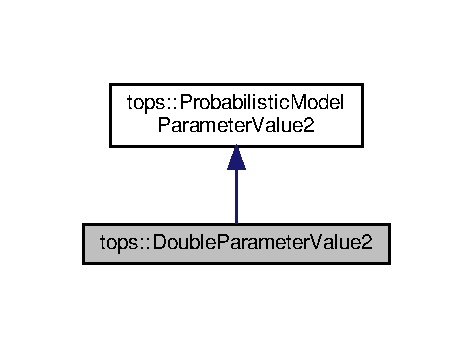
\includegraphics[width=227pt]{classtops_1_1DoubleParameterValue2__inherit__graph}
\end{center}
\end{figure}


Collaboration diagram for tops\+:\+:Double\+Parameter\+Value2\+:
\nopagebreak
\begin{figure}[H]
\begin{center}
\leavevmode
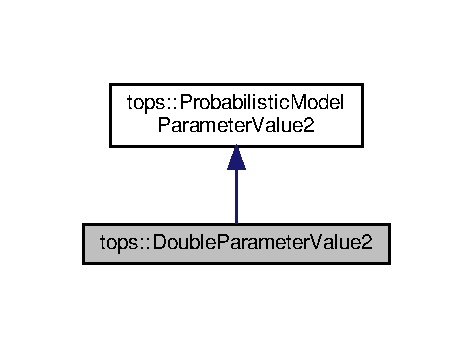
\includegraphics[width=227pt]{classtops_1_1DoubleParameterValue2__coll__graph}
\end{center}
\end{figure}
\subsection*{Public Member Functions}
\begin{DoxyCompactItemize}
\item 
\mbox{\Hypertarget{classtops_1_1DoubleParameterValue2_a2d122a816e7b3c6a7470c74e23c890ed}\label{classtops_1_1DoubleParameterValue2_a2d122a816e7b3c6a7470c74e23c890ed}} 
{\bfseries Double\+Parameter\+Value2} (double value)
\item 
\mbox{\Hypertarget{classtops_1_1DoubleParameterValue2_a6a66def34e4b40277da406f372216e6d}\label{classtops_1_1DoubleParameterValue2_a6a66def34e4b40277da406f372216e6d}} 
double {\bfseries value} ()
\item 
\mbox{\Hypertarget{classtops_1_1DoubleParameterValue2_a692fbfb2e4b4f809cad4bec4822ad41a}\label{classtops_1_1DoubleParameterValue2_a692fbfb2e4b4f809cad4bec4822ad41a}} 
virtual \hyperlink{classtops_1_1DoubleParameterValue2}{Double\+Parameter\+Value2} $\ast$ {\bfseries to\+Double\+Parameter} ()
\item 
\mbox{\Hypertarget{classtops_1_1DoubleParameterValue2_a98cc3cefaac126f16626083a3e586c12}\label{classtops_1_1DoubleParameterValue2_a98cc3cefaac126f16626083a3e586c12}} 
virtual std\+::string {\bfseries parameter\+Type} ()
\item 
\mbox{\Hypertarget{classtops_1_1DoubleParameterValue2_a803b1dc9aefe6a1abe451ad06017cfe3}\label{classtops_1_1DoubleParameterValue2_a803b1dc9aefe6a1abe451ad06017cfe3}} 
virtual std\+::string {\bfseries str} ()
\end{DoxyCompactItemize}


\subsection{Detailed Description}


Definition at line 63 of file Probabilistic\+Model\+Parameter\+Value2.\+hpp.



The documentation for this class was generated from the following files\+:\begin{DoxyCompactItemize}
\item 
src/Probabilistic\+Model\+Parameter\+Value2.\+hpp\item 
src/Probabilistic\+Model\+Parameter\+Value2.\+cpp\end{DoxyCompactItemize}

\hypertarget{classtops_1_1DoubleVectorParameterValue}{}\section{tops\+:\+:Double\+Vector\+Parameter\+Value Class Reference}
\label{classtops_1_1DoubleVectorParameterValue}\index{tops\+::\+Double\+Vector\+Parameter\+Value@{tops\+::\+Double\+Vector\+Parameter\+Value}}


double vector parameter value  




{\ttfamily \#include $<$Probabilistic\+Model\+Parameter.\+hpp$>$}



Inheritance diagram for tops\+:\+:Double\+Vector\+Parameter\+Value\+:
\nopagebreak
\begin{figure}[H]
\begin{center}
\leavevmode
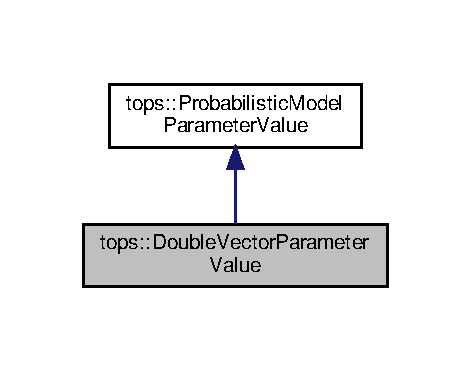
\includegraphics[width=226pt]{classtops_1_1DoubleVectorParameterValue__inherit__graph}
\end{center}
\end{figure}


Collaboration diagram for tops\+:\+:Double\+Vector\+Parameter\+Value\+:
\nopagebreak
\begin{figure}[H]
\begin{center}
\leavevmode
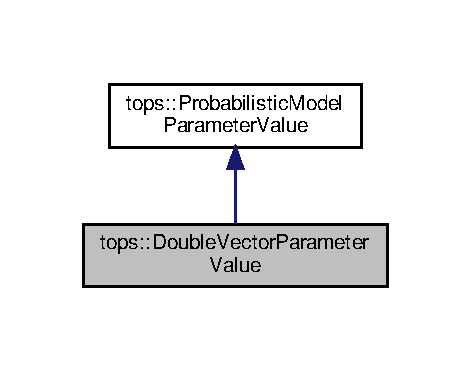
\includegraphics[width=226pt]{classtops_1_1DoubleVectorParameterValue__coll__graph}
\end{center}
\end{figure}
\subsection*{Public Member Functions}
\begin{DoxyCompactItemize}
\item 
\mbox{\Hypertarget{classtops_1_1DoubleVectorParameterValue_a2875813c348f24dd33508cf443ad9510}\label{classtops_1_1DoubleVectorParameterValue_a2875813c348f24dd33508cf443ad9510}} 
{\bfseries Double\+Vector\+Parameter\+Value} (Double\+Vector v)
\item 
\mbox{\Hypertarget{classtops_1_1DoubleVectorParameterValue_a9d6c06a590388ab33fbd98c120d0bc8a}\label{classtops_1_1DoubleVectorParameterValue_a9d6c06a590388ab33fbd98c120d0bc8a}} 
virtual void {\bfseries initialize} (Double\+Vector v)
\item 
\mbox{\Hypertarget{classtops_1_1DoubleVectorParameterValue_a997b2828d36a06aa41be0179a6963436}\label{classtops_1_1DoubleVectorParameterValue_a997b2828d36a06aa41be0179a6963436}} 
virtual Double\+Vector \& {\bfseries get\+Double\+Vector} ()
\item 
\mbox{\Hypertarget{classtops_1_1DoubleVectorParameterValue_a058e87ba54f3c1fe2e41b0273c2df0e1}\label{classtops_1_1DoubleVectorParameterValue_a058e87ba54f3c1fe2e41b0273c2df0e1}} 
virtual std\+::string {\bfseries parameter\+\_\+type} () const
\item 
\mbox{\Hypertarget{classtops_1_1DoubleVectorParameterValue_afba77bcc7858bbc0746179a277d1ac67}\label{classtops_1_1DoubleVectorParameterValue_afba77bcc7858bbc0746179a277d1ac67}} 
virtual std\+::string {\bfseries str} () const
\end{DoxyCompactItemize}


\subsection{Detailed Description}
double vector parameter value 

Definition at line 204 of file Probabilistic\+Model\+Parameter.\+hpp.



The documentation for this class was generated from the following files\+:\begin{DoxyCompactItemize}
\item 
src/Probabilistic\+Model\+Parameter.\+hpp\item 
src/Probabilistic\+Model\+Parameter.\+cpp\end{DoxyCompactItemize}

\hypertarget{classtops_1_1FactorableModel}{}\section{tops\+:\+:Factorable\+Model Class Reference}
\label{classtops_1_1FactorableModel}\index{tops\+::\+Factorable\+Model@{tops\+::\+Factorable\+Model}}


Abstract class defining models in which the likelihood of the sequence is factorable in the sense that they can be expressed as a product of terms evaluated at each position in a sequence.  




{\ttfamily \#include $<$Factorable\+Model.\+hpp$>$}



Inheritance diagram for tops\+:\+:Factorable\+Model\+:
\nopagebreak
\begin{figure}[H]
\begin{center}
\leavevmode
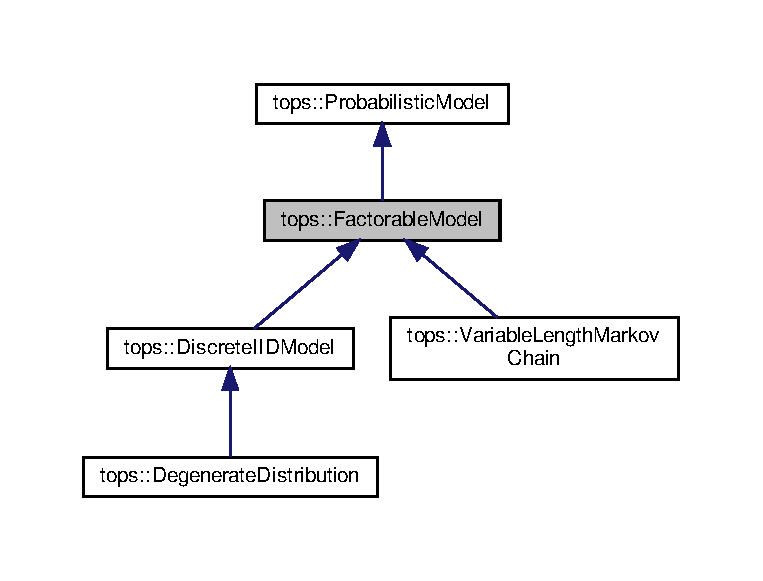
\includegraphics[width=350pt]{classtops_1_1FactorableModel__inherit__graph}
\end{center}
\end{figure}


Collaboration diagram for tops\+:\+:Factorable\+Model\+:
\nopagebreak
\begin{figure}[H]
\begin{center}
\leavevmode
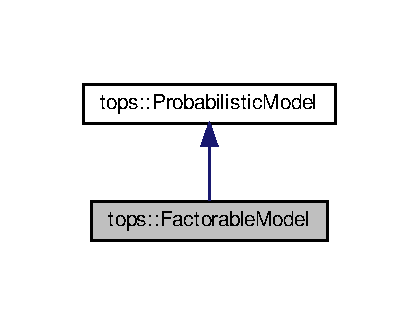
\includegraphics[width=201pt]{classtops_1_1FactorableModel__coll__graph}
\end{center}
\end{figure}
\subsection*{Public Member Functions}
\begin{DoxyCompactItemize}
\item 
\mbox{\Hypertarget{classtops_1_1FactorableModel_a17c0f432b4cfc2e1c020ee1c8e430d8a}\label{classtops_1_1FactorableModel_a17c0f432b4cfc2e1c020ee1c8e430d8a}} 
virtual double \hyperlink{classtops_1_1FactorableModel_a17c0f432b4cfc2e1c020ee1c8e430d8a}{evaluate} (const Sequence \&s, unsigned int begin, unsigned int end) const
\begin{DoxyCompactList}\small\item\em Calculates the sequence likelihood given this model. \end{DoxyCompactList}\item 
\mbox{\Hypertarget{classtops_1_1FactorableModel_ab9ba9cadb152b0090db9f71e119860c2}\label{classtops_1_1FactorableModel_ab9ba9cadb152b0090db9f71e119860c2}} 
virtual Sequence \& {\bfseries choose} (Sequence \&h, int \hyperlink{classtops_1_1ProbabilisticModel_a4e3910e9b9b848b7078e7101909ae82a}{size}) const
\item 
\mbox{\Hypertarget{classtops_1_1FactorableModel_a472415d5e60ee110433b54e7d1e61d3f}\label{classtops_1_1FactorableModel_a472415d5e60ee110433b54e7d1e61d3f}} 
virtual Sequence \& {\bfseries choose\+With\+History} (Sequence \&h, int i, int \hyperlink{classtops_1_1ProbabilisticModel_a4e3910e9b9b848b7078e7101909ae82a}{size}) const
\item 
\mbox{\Hypertarget{classtops_1_1FactorableModel_a74539e31c71e45590d76fe3173fe0d49}\label{classtops_1_1FactorableModel_a74539e31c71e45590d76fe3173fe0d49}} 
virtual double \hyperlink{classtops_1_1FactorableModel_a74539e31c71e45590d76fe3173fe0d49}{evaluate\+Position} (const Sequence \&s, unsigned int i) const =0
\begin{DoxyCompactList}\small\item\em Evaluate the position i of the sequence s. \end{DoxyCompactList}\item 
\mbox{\Hypertarget{classtops_1_1FactorableModel_a5d97e3ee9ed36526175a06c9605aab98}\label{classtops_1_1FactorableModel_a5d97e3ee9ed36526175a06c9605aab98}} 
virtual double \hyperlink{classtops_1_1FactorableModel_a5d97e3ee9ed36526175a06c9605aab98}{choose\+Position} (const Sequence \&s, int i) const =0
\begin{DoxyCompactList}\small\item\em Choose the position i of the sequence s given the subsequence before the position i. \end{DoxyCompactList}\item 
\mbox{\Hypertarget{classtops_1_1FactorableModel_a52a4240058e32f4e6ddf75fdab138a4f}\label{classtops_1_1FactorableModel_a52a4240058e32f4e6ddf75fdab138a4f}} 
virtual double {\bfseries prefix\+\_\+sum\+\_\+array\+\_\+compute} (int begin, int end)
\item 
\mbox{\Hypertarget{classtops_1_1FactorableModel_ae3f8aea76a131eb4b64bd8d9704992ca}\label{classtops_1_1FactorableModel_ae3f8aea76a131eb4b64bd8d9704992ca}} 
virtual bool {\bfseries initialize\+\_\+prefix\+\_\+sum\+\_\+array} (const Sequence \&s)
\item 
\mbox{\Hypertarget{classtops_1_1FactorableModel_afba8e107a95517fac416662c641afe65}\label{classtops_1_1FactorableModel_afba8e107a95517fac416662c641afe65}} 
virtual \hyperlink{classtops_1_1FactorableModel}{Factorable\+Model} $\ast$ {\bfseries factorable} ()
\end{DoxyCompactItemize}


\subsection{Detailed Description}
Abstract class defining models in which the likelihood of the sequence is factorable in the sense that they can be expressed as a product of terms evaluated at each position in a sequence. 

Definition at line 37 of file Factorable\+Model.\+hpp.



The documentation for this class was generated from the following files\+:\begin{DoxyCompactItemize}
\item 
src/Factorable\+Model.\+hpp\item 
src/Factorable\+Model.\+cpp\end{DoxyCompactItemize}

\hypertarget{classtops_1_1FactorableModelPrefixSumArray}{}\section{tops\+:\+:Factorable\+Model\+Prefix\+Sum\+Array Class Reference}
\label{classtops_1_1FactorableModelPrefixSumArray}\index{tops\+::\+Factorable\+Model\+Prefix\+Sum\+Array@{tops\+::\+Factorable\+Model\+Prefix\+Sum\+Array}}


This class provides an interface for working with the prefix sum arrays.  




{\ttfamily \#include $<$Factorable\+Model\+Prefix\+Sum\+Array.\+hpp$>$}



Inheritance diagram for tops\+:\+:Factorable\+Model\+Prefix\+Sum\+Array\+:
\nopagebreak
\begin{figure}[H]
\begin{center}
\leavevmode
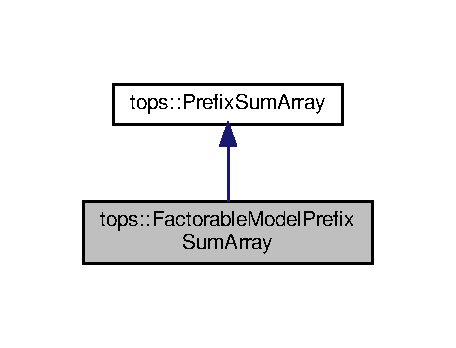
\includegraphics[width=219pt]{classtops_1_1FactorableModelPrefixSumArray__inherit__graph}
\end{center}
\end{figure}


Collaboration diagram for tops\+:\+:Factorable\+Model\+Prefix\+Sum\+Array\+:
\nopagebreak
\begin{figure}[H]
\begin{center}
\leavevmode
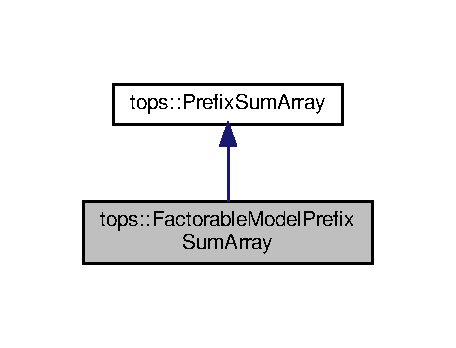
\includegraphics[width=219pt]{classtops_1_1FactorableModelPrefixSumArray__coll__graph}
\end{center}
\end{figure}
\subsection*{Public Member Functions}
\begin{DoxyCompactItemize}
\item 
\mbox{\Hypertarget{classtops_1_1FactorableModelPrefixSumArray_ac88c3a1b88fa965d9c58e5a0193d6cb7}\label{classtops_1_1FactorableModelPrefixSumArray_ac88c3a1b88fa965d9c58e5a0193d6cb7}} 
{\bfseries Factorable\+Model\+Prefix\+Sum\+Array} (\hyperlink{classtops_1_1ProbabilisticModel}{Probabilistic\+Model} $\ast$model)
\item 
\mbox{\Hypertarget{classtops_1_1FactorableModelPrefixSumArray_ad71ce1bff5834ff45717712999c96c5d}\label{classtops_1_1FactorableModelPrefixSumArray_ad71ce1bff5834ff45717712999c96c5d}} 
virtual void \hyperlink{classtops_1_1FactorableModelPrefixSumArray_ad71ce1bff5834ff45717712999c96c5d}{initialize} (const Sequence \&s)
\begin{DoxyCompactList}\small\item\em Initialize the prefix sum array. \end{DoxyCompactList}\item 
\mbox{\Hypertarget{classtops_1_1FactorableModelPrefixSumArray_a850580f8103692abc204cbf82af49c18}\label{classtops_1_1FactorableModelPrefixSumArray_a850580f8103692abc204cbf82af49c18}} 
virtual double \hyperlink{classtops_1_1FactorableModelPrefixSumArray_a850580f8103692abc204cbf82af49c18}{compute} (int begin, int end) const
\begin{DoxyCompactList}\small\item\em compute the prefix sum array \end{DoxyCompactList}\end{DoxyCompactItemize}


\subsection{Detailed Description}
This class provides an interface for working with the prefix sum arrays. 

Definition at line 39 of file Factorable\+Model\+Prefix\+Sum\+Array.\+hpp.



The documentation for this class was generated from the following files\+:\begin{DoxyCompactItemize}
\item 
src/Factorable\+Model\+Prefix\+Sum\+Array.\+hpp\item 
src/Factorable\+Model\+Prefix\+Sum\+Array.\+cpp\end{DoxyCompactItemize}

\hypertarget{classtops_1_1FastaSequenceFormat}{}\section{tops\+:\+:Fasta\+Sequence\+Format Class Reference}
\label{classtops_1_1FastaSequenceFormat}\index{tops\+::\+Fasta\+Sequence\+Format@{tops\+::\+Fasta\+Sequence\+Format}}


Fasta Format.  




{\ttfamily \#include $<$Sequence\+Format.\+hpp$>$}



Inheritance diagram for tops\+:\+:Fasta\+Sequence\+Format\+:
\nopagebreak
\begin{figure}[H]
\begin{center}
\leavevmode
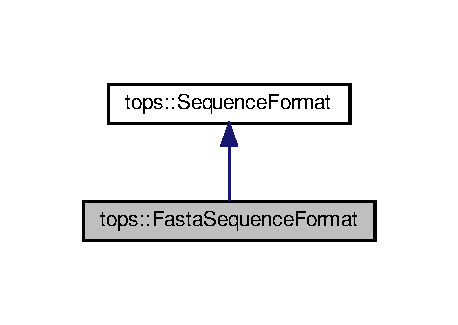
\includegraphics[width=220pt]{classtops_1_1FastaSequenceFormat__inherit__graph}
\end{center}
\end{figure}


Collaboration diagram for tops\+:\+:Fasta\+Sequence\+Format\+:
\nopagebreak
\begin{figure}[H]
\begin{center}
\leavevmode
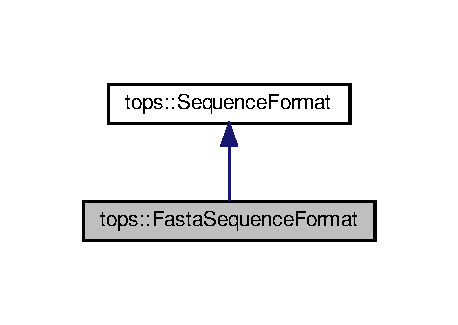
\includegraphics[width=220pt]{classtops_1_1FastaSequenceFormat__coll__graph}
\end{center}
\end{figure}
\subsection*{Public Member Functions}
\begin{DoxyCompactItemize}
\item 
\mbox{\Hypertarget{classtops_1_1FastaSequenceFormat_ad7a12724117c9e1ab9b40ec62a4c9081}\label{classtops_1_1FastaSequenceFormat_ad7a12724117c9e1ab9b40ec62a4c9081}} 
virtual std\+::ostream \& {\bfseries save\+Sequence} (std\+::ostream \&stream, \hyperlink{classtops_1_1SequenceEntry}{Sequence\+Entry} \&out)
\item 
\mbox{\Hypertarget{classtops_1_1FastaSequenceFormat_af4d170c67e5df18452968f591b39e1e0}\label{classtops_1_1FastaSequenceFormat_af4d170c67e5df18452968f591b39e1e0}} 
virtual std\+::istream \& {\bfseries read\+Sequence} (std\+::istream \&stream, \hyperlink{classtops_1_1SequenceEntry}{Sequence\+Entry} \&in)
\end{DoxyCompactItemize}


\subsection{Detailed Description}
Fasta Format. 

Definition at line 48 of file Sequence\+Format.\+hpp.



The documentation for this class was generated from the following files\+:\begin{DoxyCompactItemize}
\item 
src/Sequence\+Format.\+hpp\item 
src/Sequence\+Format.\+cpp\end{DoxyCompactItemize}

\hypertarget{classtops_1_1FixedSequenceAtPosition}{}\section{tops\+:\+:Fixed\+Sequence\+At\+Position Class Reference}
\label{classtops_1_1FixedSequenceAtPosition}\index{tops\+::\+Fixed\+Sequence\+At\+Position@{tops\+::\+Fixed\+Sequence\+At\+Position}}


A decorator that forces the emission of the same sequence at a fixed position of the sequence.  




{\ttfamily \#include $<$Fixed\+Sequence\+At\+Position.\+hpp$>$}



Inheritance diagram for tops\+:\+:Fixed\+Sequence\+At\+Position\+:
\nopagebreak
\begin{figure}[H]
\begin{center}
\leavevmode
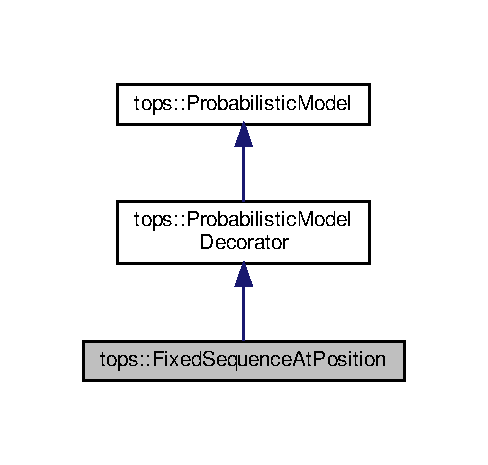
\includegraphics[width=234pt]{classtops_1_1FixedSequenceAtPosition__inherit__graph}
\end{center}
\end{figure}


Collaboration diagram for tops\+:\+:Fixed\+Sequence\+At\+Position\+:
\nopagebreak
\begin{figure}[H]
\begin{center}
\leavevmode
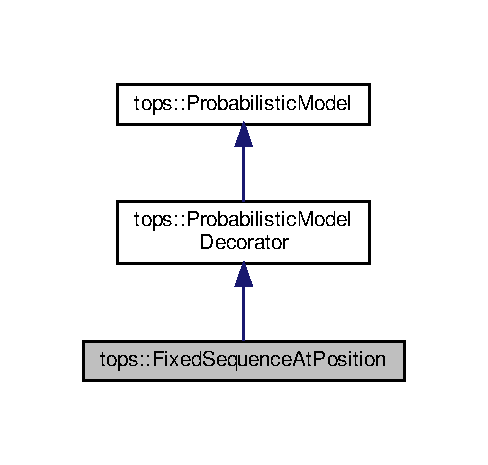
\includegraphics[width=234pt]{classtops_1_1FixedSequenceAtPosition__coll__graph}
\end{center}
\end{figure}
\subsection*{Public Member Functions}
\begin{DoxyCompactItemize}
\item 
\mbox{\Hypertarget{classtops_1_1FixedSequenceAtPosition_afc84dd484d286f246a7536d6f50feb93}\label{classtops_1_1FixedSequenceAtPosition_afc84dd484d286f246a7536d6f50feb93}} 
{\bfseries Fixed\+Sequence\+At\+Position} (Probabilistic\+Model\+Ptr m)
\item 
\mbox{\Hypertarget{classtops_1_1FixedSequenceAtPosition_a5337554ef494d0dce741580266b8cbbd}\label{classtops_1_1FixedSequenceAtPosition_a5337554ef494d0dce741580266b8cbbd}} 
virtual void {\bfseries initialize} (int position, Sequence sequence, Discrete\+I\+I\+D\+Model\+Ptr distr)
\item 
\mbox{\Hypertarget{classtops_1_1FixedSequenceAtPosition_a18c28305c607a6d0a4699dd5244ad8d0}\label{classtops_1_1FixedSequenceAtPosition_a18c28305c607a6d0a4699dd5244ad8d0}} 
virtual double \hyperlink{classtops_1_1FixedSequenceAtPosition_a18c28305c607a6d0a4699dd5244ad8d0}{evaluate} (const Sequence \&s, unsigned int begin, unsigned int end) const
\begin{DoxyCompactList}\small\item\em Calculates the sequence likelihood given this model. \end{DoxyCompactList}\item 
\mbox{\Hypertarget{classtops_1_1FixedSequenceAtPosition_a3e50c13ff092961851feadd5f345943e}\label{classtops_1_1FixedSequenceAtPosition_a3e50c13ff092961851feadd5f345943e}} 
virtual Sequence \& {\bfseries choose} (Sequence \&h, int \hyperlink{classtops_1_1ProbabilisticModel_a4e3910e9b9b848b7078e7101909ae82a}{size}) const
\item 
\mbox{\Hypertarget{classtops_1_1FixedSequenceAtPosition_a90c619825f8973acc053f2b3fee35497}\label{classtops_1_1FixedSequenceAtPosition_a90c619825f8973acc053f2b3fee35497}} 
virtual Sequence \& {\bfseries choose} (Sequence \&h, int initial\+\_\+phase, int \hyperlink{classtops_1_1ProbabilisticModel_a4e3910e9b9b848b7078e7101909ae82a}{size}) const
\item 
\mbox{\Hypertarget{classtops_1_1FixedSequenceAtPosition_a25deb5048f3e1dd278a923c2bfce50bf}\label{classtops_1_1FixedSequenceAtPosition_a25deb5048f3e1dd278a923c2bfce50bf}} 
virtual Sequence \& {\bfseries choose} (Sequence \&h, Sequence \&path, int \hyperlink{classtops_1_1ProbabilisticModel_a4e3910e9b9b848b7078e7101909ae82a}{size}) const
\item 
\mbox{\Hypertarget{classtops_1_1FixedSequenceAtPosition_a241d9315ae90fe8d8f57c8072af72a22}\label{classtops_1_1FixedSequenceAtPosition_a241d9315ae90fe8d8f57c8072af72a22}} 
virtual Sequence \& {\bfseries choose} (Sequence \&h, Sequence \&path, int i, int \hyperlink{classtops_1_1ProbabilisticModel_a4e3910e9b9b848b7078e7101909ae82a}{size}) const
\item 
\mbox{\Hypertarget{classtops_1_1FixedSequenceAtPosition_ad5cfee86e160eb7249cd1f850aa53adf}\label{classtops_1_1FixedSequenceAtPosition_ad5cfee86e160eb7249cd1f850aa53adf}} 
virtual Sequence \& {\bfseries choose\+With\+History} (Sequence \&h, int i, int \hyperlink{classtops_1_1ProbabilisticModel_a4e3910e9b9b848b7078e7101909ae82a}{size}) const
\item 
\mbox{\Hypertarget{classtops_1_1FixedSequenceAtPosition_a58e48dfdfdba8a8269508217fe5e0e6a}\label{classtops_1_1FixedSequenceAtPosition_a58e48dfdfdba8a8269508217fe5e0e6a}} 
virtual Sequence \& {\bfseries choose\+With\+History} (Sequence \&h, int i, int phase, int \hyperlink{classtops_1_1ProbabilisticModel_a4e3910e9b9b848b7078e7101909ae82a}{size}) const
\item 
\mbox{\Hypertarget{classtops_1_1FixedSequenceAtPosition_a1600948006e576c46958c69eb3b9dde9}\label{classtops_1_1FixedSequenceAtPosition_a1600948006e576c46958c69eb3b9dde9}} 
virtual double {\bfseries prefix\+\_\+sum\+\_\+array\+\_\+compute} (int begin, int end)
\item 
\mbox{\Hypertarget{classtops_1_1FixedSequenceAtPosition_a7aa2ee2c289eb7538c8fff063b17fdbc}\label{classtops_1_1FixedSequenceAtPosition_a7aa2ee2c289eb7538c8fff063b17fdbc}} 
virtual double {\bfseries prefix\+\_\+sum\+\_\+array\+\_\+compute} (int begin, int end, int phase)
\item 
\mbox{\Hypertarget{classtops_1_1FixedSequenceAtPosition_acb1f8bebd2815c580c66526c55b292e7}\label{classtops_1_1FixedSequenceAtPosition_acb1f8bebd2815c580c66526c55b292e7}} 
virtual bool {\bfseries initialize\+\_\+prefix\+\_\+sum\+\_\+array} (const Sequence \&s, int phase)
\item 
\mbox{\Hypertarget{classtops_1_1FixedSequenceAtPosition_a61cf8b9a9e91b1785fe52f05fc6d041e}\label{classtops_1_1FixedSequenceAtPosition_a61cf8b9a9e91b1785fe52f05fc6d041e}} 
virtual bool {\bfseries initialize\+\_\+prefix\+\_\+sum\+\_\+array} (const Sequence \&s)
\item 
\mbox{\Hypertarget{classtops_1_1FixedSequenceAtPosition_a55c81be8635c092f980689e7fa723998}\label{classtops_1_1FixedSequenceAtPosition_a55c81be8635c092f980689e7fa723998}} 
virtual std\+::string \hyperlink{classtops_1_1FixedSequenceAtPosition_a55c81be8635c092f980689e7fa723998}{str} () const
\begin{DoxyCompactList}\small\item\em returns the string representation of the model \end{DoxyCompactList}\item 
\mbox{\Hypertarget{classtops_1_1FixedSequenceAtPosition_acc3c6985dbd22612f13e0a7e1f485c2d}\label{classtops_1_1FixedSequenceAtPosition_acc3c6985dbd22612f13e0a7e1f485c2d}} 
std\+::string \hyperlink{classtops_1_1FixedSequenceAtPosition_acc3c6985dbd22612f13e0a7e1f485c2d}{model\+\_\+name} () const
\begin{DoxyCompactList}\small\item\em returns the model name \end{DoxyCompactList}\end{DoxyCompactItemize}


\subsection{Detailed Description}
A decorator that forces the emission of the same sequence at a fixed position of the sequence. 

Definition at line 34 of file Fixed\+Sequence\+At\+Position.\+hpp.



The documentation for this class was generated from the following files\+:\begin{DoxyCompactItemize}
\item 
src/Fixed\+Sequence\+At\+Position.\+hpp\item 
src/Fixed\+Sequence\+At\+Position.\+cpp\end{DoxyCompactItemize}

\hypertarget{classtops_1_1FixedSequenceAtPositionCreator}{}\section{tops\+:\+:Fixed\+Sequence\+At\+Position\+Creator Class Reference}
\label{classtops_1_1FixedSequenceAtPositionCreator}\index{tops\+::\+Fixed\+Sequence\+At\+Position\+Creator@{tops\+::\+Fixed\+Sequence\+At\+Position\+Creator}}


Inheritance diagram for tops\+:\+:Fixed\+Sequence\+At\+Position\+Creator\+:
\nopagebreak
\begin{figure}[H]
\begin{center}
\leavevmode
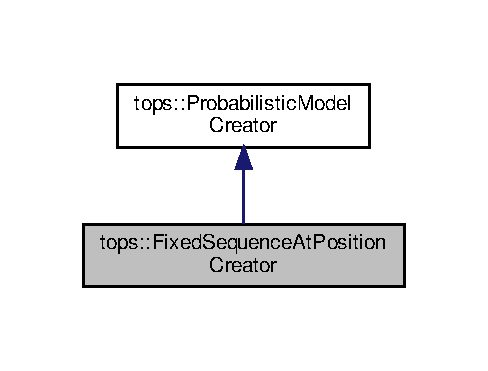
\includegraphics[width=234pt]{classtops_1_1FixedSequenceAtPositionCreator__inherit__graph}
\end{center}
\end{figure}


Collaboration diagram for tops\+:\+:Fixed\+Sequence\+At\+Position\+Creator\+:
\nopagebreak
\begin{figure}[H]
\begin{center}
\leavevmode
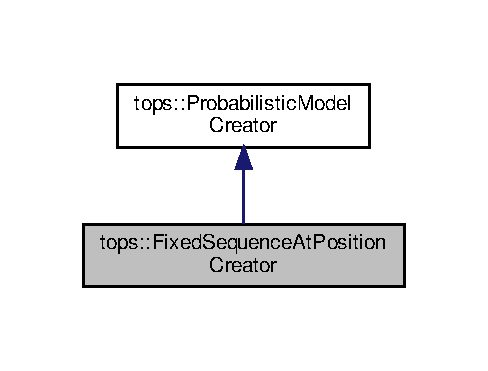
\includegraphics[width=234pt]{classtops_1_1FixedSequenceAtPositionCreator__coll__graph}
\end{center}
\end{figure}
\subsection*{Public Member Functions}
\begin{DoxyCompactItemize}
\item 
virtual Probabilistic\+Model\+Ptr \hyperlink{classtops_1_1FixedSequenceAtPositionCreator_af4daf171afbef0494ee98f9877ff1787}{create} (\hyperlink{classtops_1_1ProbabilisticModelParameters}{Probabilistic\+Model\+Parameters} \&parameters) const
\begin{DoxyCompactList}\small\item\em Creates a probability model. \end{DoxyCompactList}\end{DoxyCompactItemize}


\subsection{Detailed Description}


Definition at line 33 of file Fixed\+Sequence\+At\+Position\+Creator.\+hpp.



\subsection{Member Function Documentation}
\mbox{\Hypertarget{classtops_1_1FixedSequenceAtPositionCreator_af4daf171afbef0494ee98f9877ff1787}\label{classtops_1_1FixedSequenceAtPositionCreator_af4daf171afbef0494ee98f9877ff1787}} 
\index{tops\+::\+Fixed\+Sequence\+At\+Position\+Creator@{tops\+::\+Fixed\+Sequence\+At\+Position\+Creator}!create@{create}}
\index{create@{create}!tops\+::\+Fixed\+Sequence\+At\+Position\+Creator@{tops\+::\+Fixed\+Sequence\+At\+Position\+Creator}}
\subsubsection{\texorpdfstring{create()}{create()}}
{\footnotesize\ttfamily Probabilistic\+Model\+Ptr tops\+::\+Fixed\+Sequence\+At\+Position\+Creator\+::create (\begin{DoxyParamCaption}\item[{\hyperlink{classtops_1_1ProbabilisticModelParameters}{Probabilistic\+Model\+Parameters} \&}]{parameters }\end{DoxyParamCaption}) const\hspace{0.3cm}{\ttfamily [virtual]}}



Creates a probability model. 


\begin{DoxyParams}{Parameters}
{\em parameters} & is a set of parameters that is utilized to build the model \\
\hline
\end{DoxyParams}


Reimplemented from \hyperlink{classtops_1_1ProbabilisticModelCreator_afed6c8ffa45fff446bdaa8b533da8f7c}{tops\+::\+Probabilistic\+Model\+Creator}.



Definition at line 32 of file Fixed\+Sequence\+At\+Position\+Creator.\+cpp.


\begin{DoxyCode}
32                                                                                                            
          \{
33     ProbabilisticModelParameterValuePtr positionpar = parameters.getMandatoryParameterValue(\textcolor{stringliteral}{"position"});
34     ProbabilisticModelParameterValuePtr sequencepar = parameters.getMandatoryParameterValue(\textcolor{stringliteral}{"sequence"});
35     ProbabilisticModelParameterValuePtr probabilitypar = parameters.getMandatoryParameterValue(\textcolor{stringliteral}{"probability
      "});
36     ProbabilisticModelParameterValuePtr modelpar = parameters.getMandatoryParameterValue(\textcolor{stringliteral}{"model"});
37     boost::regex sep(\textcolor{stringliteral}{" "});
38     std::vector<std::string> seqstr;
39     split\_regex(sequencepar->getString(), seqstr,  sep);
40 
41 
42     \textcolor{keywordtype}{int} position = positionpar->getInt();
43     std::vector<double> probs;
44     probs.push\_back(probabilitypar->getDouble());
45     probs.push\_back(1.0 - probabilitypar->getDouble());
46     ProbabilisticModelCreatorClient creator;
47     ConfigurationReader reader;
48     std::string modelstr = modelpar->getString();
49 
50     ProbabilisticModelPtr m ;
51     \textcolor{keywordflow}{if}((modelstr.size() > 0) && (modelstr[0] == \textcolor{charliteral}{'['}) )\{
52       modelstr = modelstr.substr(1, modelstr.size() -2 );
53       reader.load(modelstr);
54       ProbabilisticModelParametersPtr par = reader.parameters();
55       m = creator.create(*par);
56     \} \textcolor{keywordflow}{else}
57       \{
58         m = creator.create(modelstr) ;
59         \textcolor{keywordflow}{if}(m == NULL) \{
60           std::cerr << \textcolor{stringliteral}{"Can not load model file "} << modelstr<< \textcolor{stringliteral}{"!"} << std::endl;
61           exit(-1);
62         \}
63       \}
64     FixedSequenceAtPositionPtr decorator = FixedSequenceAtPositionPtr(\textcolor{keyword}{new} FixedSequenceAtPosition(m));
65 
66     DiscreteIIDModelPtr distr = DiscreteIIDModelPtr(\textcolor{keyword}{new} DiscreteIIDModel(probs));
67     AlphabetPtr alpha = m->alphabet();
68     SequenceFactory factory(alpha);
69     Sequence sequence = factory.createSequence(seqstr);
70     decorator->initialize(position, sequence, distr);
71     decorator->setAlphabet(m->alphabet());
72     decorator->subModelName(modelstr);
73     \textcolor{keywordflow}{return} decorator;
74   \}
\end{DoxyCode}


The documentation for this class was generated from the following files\+:\begin{DoxyCompactItemize}
\item 
src/Fixed\+Sequence\+At\+Position\+Creator.\+hpp\item 
src/Fixed\+Sequence\+At\+Position\+Creator.\+cpp\end{DoxyCompactItemize}

\hypertarget{classtops_1_1Gap1State}{}\section{tops\+:\+:Gap1\+State Class Reference}
\label{classtops_1_1Gap1State}\index{tops\+::\+Gap1\+State@{tops\+::\+Gap1\+State}}


Inheritance diagram for tops\+:\+:Gap1\+State\+:
\nopagebreak
\begin{figure}[H]
\begin{center}
\leavevmode
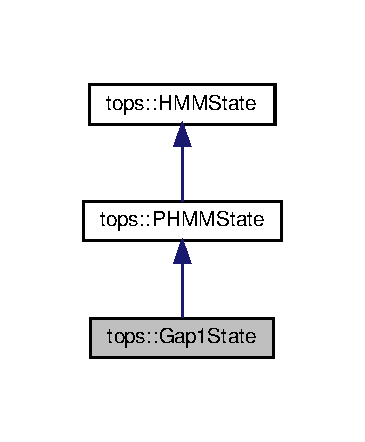
\includegraphics[width=175pt]{classtops_1_1Gap1State__inherit__graph}
\end{center}
\end{figure}


Collaboration diagram for tops\+:\+:Gap1\+State\+:
\nopagebreak
\begin{figure}[H]
\begin{center}
\leavevmode
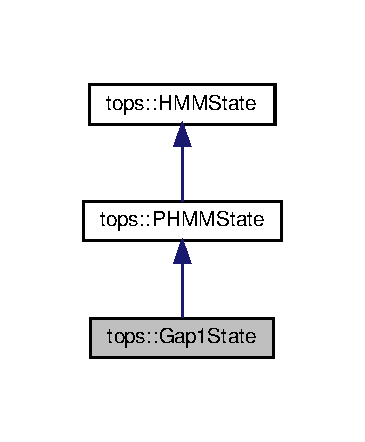
\includegraphics[width=175pt]{classtops_1_1Gap1State__coll__graph}
\end{center}
\end{figure}
\subsection*{Public Member Functions}
\begin{DoxyCompactItemize}
\item 
\mbox{\Hypertarget{classtops_1_1Gap1State_a2a9530e58e72bd1fcd45334232ea30b9}\label{classtops_1_1Gap1State_a2a9530e58e72bd1fcd45334232ea30b9}} 
{\bfseries Gap1\+State} (int id, Symbol\+Ptr name, Discrete\+I\+I\+D\+Model\+Ptr emission, Discrete\+I\+I\+D\+Model\+Ptr transitions, Int\+Vector i\+Transitions, Int\+Vector o\+Transitions)
\item 
\mbox{\Hypertarget{classtops_1_1Gap1State_a893baf7ce3eb45b398d59c57dfcc97f6}\label{classtops_1_1Gap1State_a893baf7ce3eb45b398d59c57dfcc97f6}} 
void {\bfseries forward\+Sum} (vector$<$ P\+H\+M\+M\+State\+Ptr $>$ \&states, const Sequence \&seq1, const Sequence \&seq2, vector$<$ Matrix $>$ \&a, int i, int j, int gap\+\_\+id, int begin\+\_\+id)
\item 
\mbox{\Hypertarget{classtops_1_1Gap1State_a24d5685c33fb3902b92aee9e718de7ee}\label{classtops_1_1Gap1State_a24d5685c33fb3902b92aee9e718de7ee}} 
void {\bfseries backward\+Sum} (vector$<$ P\+H\+M\+M\+State\+Ptr $>$ \&states, const Sequence \&seq1, const Sequence \&seq2, vector$<$ Matrix $>$ \&a, int i, int j, int gap\+\_\+id, int curr\+State\+Id, double $\ast$accumulator)
\item 
\mbox{\Hypertarget{classtops_1_1Gap1State_ad509beb6d2f6d573aca8c0a6152eefe5}\label{classtops_1_1Gap1State_ad509beb6d2f6d573aca8c0a6152eefe5}} 
void {\bfseries post\+Prob\+Sum} (f\+Matrix \&pp\+Match, f\+Matrix \&pp\+Gap1, f\+Matrix \&pp\+Gap2, Matrix \&alpha, Matrix \&beta, double full, int i, int j)
\end{DoxyCompactItemize}
\subsection*{Additional Inherited Members}


\subsection{Detailed Description}


Definition at line 136 of file Pair\+Hidden\+Markov\+Model.\+hpp.



The documentation for this class was generated from the following files\+:\begin{DoxyCompactItemize}
\item 
src/Pair\+Hidden\+Markov\+Model.\+hpp\item 
src/Pair\+Hidden\+Markov\+Model.\+cpp\end{DoxyCompactItemize}

\hypertarget{classtops_1_1Gap2State}{}\section{tops\+:\+:Gap2\+State Class Reference}
\label{classtops_1_1Gap2State}\index{tops\+::\+Gap2\+State@{tops\+::\+Gap2\+State}}


Inheritance diagram for tops\+:\+:Gap2\+State\+:
\nopagebreak
\begin{figure}[H]
\begin{center}
\leavevmode
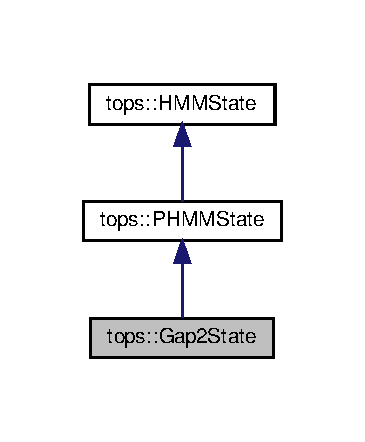
\includegraphics[width=175pt]{classtops_1_1Gap2State__inherit__graph}
\end{center}
\end{figure}


Collaboration diagram for tops\+:\+:Gap2\+State\+:
\nopagebreak
\begin{figure}[H]
\begin{center}
\leavevmode
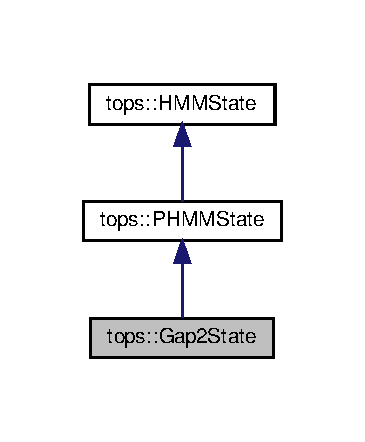
\includegraphics[width=175pt]{classtops_1_1Gap2State__coll__graph}
\end{center}
\end{figure}
\subsection*{Public Member Functions}
\begin{DoxyCompactItemize}
\item 
\mbox{\Hypertarget{classtops_1_1Gap2State_a1f4a9a225a9dcefc67d364083b59fc09}\label{classtops_1_1Gap2State_a1f4a9a225a9dcefc67d364083b59fc09}} 
{\bfseries Gap2\+State} (int id, Symbol\+Ptr name, Discrete\+I\+I\+D\+Model\+Ptr emission, Discrete\+I\+I\+D\+Model\+Ptr transitions, Int\+Vector i\+Transitions, Int\+Vector o\+Transitions)
\item 
\mbox{\Hypertarget{classtops_1_1Gap2State_a19924067024ba8df5b31080d47e85115}\label{classtops_1_1Gap2State_a19924067024ba8df5b31080d47e85115}} 
void {\bfseries forward\+Sum} (vector$<$ P\+H\+M\+M\+State\+Ptr $>$ \&states, const Sequence \&seq1, const Sequence \&seq2, vector$<$ Matrix $>$ \&a, int i, int j, int gap\+\_\+id, int begin\+\_\+id)
\item 
\mbox{\Hypertarget{classtops_1_1Gap2State_a0da1865f5076ad454cc6fe604f00e112}\label{classtops_1_1Gap2State_a0da1865f5076ad454cc6fe604f00e112}} 
void {\bfseries backward\+Sum} (vector$<$ P\+H\+M\+M\+State\+Ptr $>$ \&states, const Sequence \&seq1, const Sequence \&seq2, vector$<$ Matrix $>$ \&a, int i, int j, int gap\+\_\+id, int curr\+State\+Id, double $\ast$accumulator)
\item 
\mbox{\Hypertarget{classtops_1_1Gap2State_a9e593194fb1a6a1cb9c2b970644f7f5d}\label{classtops_1_1Gap2State_a9e593194fb1a6a1cb9c2b970644f7f5d}} 
void {\bfseries post\+Prob\+Sum} (f\+Matrix \&pp\+Match, f\+Matrix \&pp\+Gap1, f\+Matrix \&pp\+Gap2, Matrix \&alpha, Matrix \&beta, double full, int i, int j)
\end{DoxyCompactItemize}
\subsection*{Additional Inherited Members}


\subsection{Detailed Description}


Definition at line 154 of file Pair\+Hidden\+Markov\+Model.\+hpp.



The documentation for this class was generated from the following files\+:\begin{DoxyCompactItemize}
\item 
src/Pair\+Hidden\+Markov\+Model.\+hpp\item 
src/Pair\+Hidden\+Markov\+Model.\+cpp\end{DoxyCompactItemize}

\hypertarget{classtops_1_1GeneralizedHiddenMarkovModel}{}\section{tops\+:\+:Generalized\+Hidden\+Markov\+Model Class Reference}
\label{classtops_1_1GeneralizedHiddenMarkovModel}\index{tops\+::\+Generalized\+Hidden\+Markov\+Model@{tops\+::\+Generalized\+Hidden\+Markov\+Model}}


This is a class representing Hidden semi-\/\+Markov Models.  




{\ttfamily \#include $<$Generalized\+Hidden\+Markov\+Model.\+hpp$>$}



Inheritance diagram for tops\+:\+:Generalized\+Hidden\+Markov\+Model\+:
\nopagebreak
\begin{figure}[H]
\begin{center}
\leavevmode
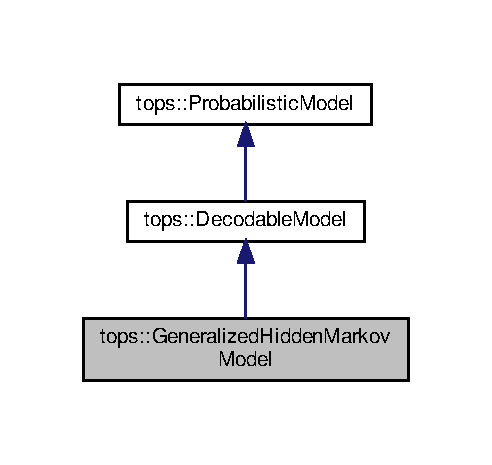
\includegraphics[width=236pt]{classtops_1_1GeneralizedHiddenMarkovModel__inherit__graph}
\end{center}
\end{figure}


Collaboration diagram for tops\+:\+:Generalized\+Hidden\+Markov\+Model\+:
\nopagebreak
\begin{figure}[H]
\begin{center}
\leavevmode
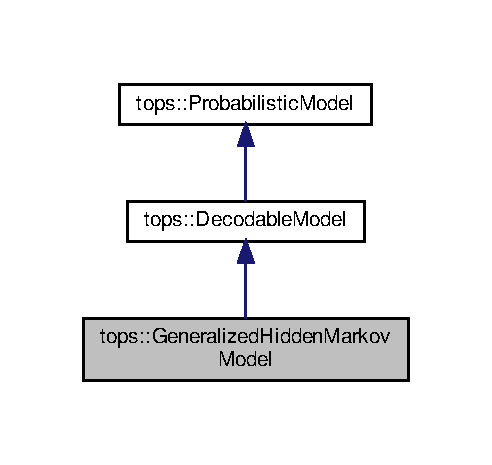
\includegraphics[width=236pt]{classtops_1_1GeneralizedHiddenMarkovModel__coll__graph}
\end{center}
\end{figure}
\subsection*{Public Member Functions}
\begin{DoxyCompactItemize}
\item 
\mbox{\Hypertarget{classtops_1_1GeneralizedHiddenMarkovModel_acbe3287fb655a591d39908680e0fbc07}\label{classtops_1_1GeneralizedHiddenMarkovModel_acbe3287fb655a591d39908680e0fbc07}} 
void {\bfseries fix\+States\+Predecessor\+Successor} ()
\item 
\mbox{\Hypertarget{classtops_1_1GeneralizedHiddenMarkovModel_a2cfc12de31de7744a5e08aa28f0cb220}\label{classtops_1_1GeneralizedHiddenMarkovModel_a2cfc12de31de7744a5e08aa28f0cb220}} 
virtual double {\bfseries inefficient\+\_\+forward} (const Sequence \&s, Matrix \&alpha) const
\item 
\mbox{\Hypertarget{classtops_1_1GeneralizedHiddenMarkovModel_a7e7f9b05017d842f85efe10f52b4a0a0}\label{classtops_1_1GeneralizedHiddenMarkovModel_a7e7f9b05017d842f85efe10f52b4a0a0}} 
virtual std\+::string {\bfseries print\+\_\+graph} () const
\item 
\mbox{\Hypertarget{classtops_1_1GeneralizedHiddenMarkovModel_a58c2de32d633890c97dee00301d5534c}\label{classtops_1_1GeneralizedHiddenMarkovModel_a58c2de32d633890c97dee00301d5534c}} 
virtual double \hyperlink{classtops_1_1GeneralizedHiddenMarkovModel_a58c2de32d633890c97dee00301d5534c}{forward} (const Sequence \&s, Matrix \&alpha) const
\begin{DoxyCompactList}\small\item\em Forward algorithm. \end{DoxyCompactList}\item 
\mbox{\Hypertarget{classtops_1_1GeneralizedHiddenMarkovModel_a073afb87466f0fc9b2fc52e94bae9269}\label{classtops_1_1GeneralizedHiddenMarkovModel_a073afb87466f0fc9b2fc52e94bae9269}} 
virtual double \hyperlink{classtops_1_1GeneralizedHiddenMarkovModel_a073afb87466f0fc9b2fc52e94bae9269}{backward} (const Sequence \&s, Matrix \&beta) const
\begin{DoxyCompactList}\small\item\em Backward algorithm. \end{DoxyCompactList}\item 
\mbox{\Hypertarget{classtops_1_1GeneralizedHiddenMarkovModel_a9c708d79292d082a2a1c0618d662fad7}\label{classtops_1_1GeneralizedHiddenMarkovModel_a9c708d79292d082a2a1c0618d662fad7}} 
virtual void {\bfseries posterior\+Probabilities\+With\+Classes} (const Sequence \&s, Sparse\+Matrix\+Ptr probabilities) const
\item 
\mbox{\Hypertarget{classtops_1_1GeneralizedHiddenMarkovModel_aba67124b630b7e629247eaa01342f9a1}\label{classtops_1_1GeneralizedHiddenMarkovModel_aba67124b630b7e629247eaa01342f9a1}} 
virtual void {\bfseries posterior\+Probabilities\+No\+Classes} (const Sequence \&s, f\+Matrix \&probabilities) const
\item 
\mbox{\Hypertarget{classtops_1_1GeneralizedHiddenMarkovModel_adbaf1c508674368629dc13e1e9d24896}\label{classtops_1_1GeneralizedHiddenMarkovModel_adbaf1c508674368629dc13e1e9d24896}} 
void {\bfseries posterior\+Probabilities} (const Sequence \&s, f\+Matrix \&post\+Probs) const
\item 
\mbox{\Hypertarget{classtops_1_1GeneralizedHiddenMarkovModel_a05f89824bf4b86e60389eb81bec11014}\label{classtops_1_1GeneralizedHiddenMarkovModel_a05f89824bf4b86e60389eb81bec11014}} 
float {\bfseries M\+E\+A\+Pred} (const Sequence \&s, Sequence \&path)
\item 
\mbox{\Hypertarget{classtops_1_1GeneralizedHiddenMarkovModel_a9da68c98f3541c708e619617a71277b0}\label{classtops_1_1GeneralizedHiddenMarkovModel_a9da68c98f3541c708e619617a71277b0}} 
float {\bfseries M\+E\+A\+Pred} (const Sequence \&s, Sequence \&path, Sparse\+Matrix\+Ptr pp\+Pred)
\item 
\mbox{\Hypertarget{classtops_1_1GeneralizedHiddenMarkovModel_a3002226ce58a1a1add9473247a489e26}\label{classtops_1_1GeneralizedHiddenMarkovModel_a3002226ce58a1a1add9473247a489e26}} 
virtual void {\bfseries set\+Num\+Classes} (int nclasses)
\item 
\mbox{\Hypertarget{classtops_1_1GeneralizedHiddenMarkovModel_a3a2b7a4a58b562f79e323bb08d6466ff}\label{classtops_1_1GeneralizedHiddenMarkovModel_a3a2b7a4a58b562f79e323bb08d6466ff}} 
virtual int {\bfseries get\+Num\+Classes} ()
\item 
\mbox{\Hypertarget{classtops_1_1GeneralizedHiddenMarkovModel_ab2c66b9df98c2a06afb2101c4eff9fe3}\label{classtops_1_1GeneralizedHiddenMarkovModel_ab2c66b9df98c2a06afb2101c4eff9fe3}} 
virtual double \hyperlink{classtops_1_1GeneralizedHiddenMarkovModel_ab2c66b9df98c2a06afb2101c4eff9fe3}{viterbi} (const Sequence \&s, Sequence \&path, Matrix \&gamma) const
\begin{DoxyCompactList}\small\item\em Viterbi algorithm. \end{DoxyCompactList}\item 
\mbox{\Hypertarget{classtops_1_1GeneralizedHiddenMarkovModel_abb20e8b6109fb2e677a84c14a4cd4b1b}\label{classtops_1_1GeneralizedHiddenMarkovModel_abb20e8b6109fb2e677a84c14a4cd4b1b}} 
virtual void \hyperlink{classtops_1_1GeneralizedHiddenMarkovModel_abb20e8b6109fb2e677a84c14a4cd4b1b}{choose\+Path} (const Sequence \&s, Sequence \&path)
\begin{DoxyCompactList}\small\item\em Choose a path given a sequence\+\_\+length. \end{DoxyCompactList}\item 
\mbox{\Hypertarget{classtops_1_1GeneralizedHiddenMarkovModel_afb005c39b26f64015b8b00d86a992e61}\label{classtops_1_1GeneralizedHiddenMarkovModel_afb005c39b26f64015b8b00d86a992e61}} 
virtual void {\bfseries initialize\+Choose\+Path\+Algorithm} (const Sequence \&s)
\item 
\mbox{\Hypertarget{classtops_1_1GeneralizedHiddenMarkovModel_a9cc86a386fb72dc574bc4ee990c48e1c}\label{classtops_1_1GeneralizedHiddenMarkovModel_a9cc86a386fb72dc574bc4ee990c48e1c}} 
virtual double \hyperlink{classtops_1_1GeneralizedHiddenMarkovModel_a9cc86a386fb72dc574bc4ee990c48e1c}{\+\_\+viterbi} (const Sequence \&s, Sequence \&path, Matrix \&gamma) const
\begin{DoxyCompactList}\small\item\em Inefficient Viterbi algorithm. \end{DoxyCompactList}\item 
\mbox{\Hypertarget{classtops_1_1GeneralizedHiddenMarkovModel_a233bb11a876558c449713e274f0f7f6c}\label{classtops_1_1GeneralizedHiddenMarkovModel_a233bb11a876558c449713e274f0f7f6c}} 
virtual Sequence \& \hyperlink{classtops_1_1GeneralizedHiddenMarkovModel_a233bb11a876558c449713e274f0f7f6c}{choose\+Observation} (Sequence \&h, int i, int state) const
\begin{DoxyCompactList}\small\item\em Choose the observation given a state. \end{DoxyCompactList}\item 
\mbox{\Hypertarget{classtops_1_1GeneralizedHiddenMarkovModel_ab7eb7993934b64eec491e956f9901b51}\label{classtops_1_1GeneralizedHiddenMarkovModel_ab7eb7993934b64eec491e956f9901b51}} 
virtual int \hyperlink{classtops_1_1GeneralizedHiddenMarkovModel_ab7eb7993934b64eec491e956f9901b51}{choose\+State} (int state) const
\begin{DoxyCompactList}\small\item\em Choose a state. \end{DoxyCompactList}\item 
\mbox{\Hypertarget{classtops_1_1GeneralizedHiddenMarkovModel_ae42041710ca7d90aeddfa139225a61fa}\label{classtops_1_1GeneralizedHiddenMarkovModel_ae42041710ca7d90aeddfa139225a61fa}} 
virtual int \hyperlink{classtops_1_1GeneralizedHiddenMarkovModel_ae42041710ca7d90aeddfa139225a61fa}{choose\+First\+State} () const
\begin{DoxyCompactList}\small\item\em Choose the initial state. \end{DoxyCompactList}\item 
\mbox{\Hypertarget{classtops_1_1GeneralizedHiddenMarkovModel_a7e3a1ae6f422ed74abb52c5f1ec4f5b6}\label{classtops_1_1GeneralizedHiddenMarkovModel_a7e3a1ae6f422ed74abb52c5f1ec4f5b6}} 
virtual Discrete\+I\+I\+D\+Model\+Ptr \hyperlink{classtops_1_1GeneralizedHiddenMarkovModel_a7e3a1ae6f422ed74abb52c5f1ec4f5b6}{get\+Initial\+Probabilities} () const
\begin{DoxyCompactList}\small\item\em Choose the initial state. \end{DoxyCompactList}\item 
\mbox{\Hypertarget{classtops_1_1GeneralizedHiddenMarkovModel_aaa5ecf2361626214250973423601232c}\label{classtops_1_1GeneralizedHiddenMarkovModel_aaa5ecf2361626214250973423601232c}} 
virtual std\+::string \hyperlink{classtops_1_1GeneralizedHiddenMarkovModel_aaa5ecf2361626214250973423601232c}{get\+State\+Name} (int state) const
\begin{DoxyCompactList}\small\item\em Get state name. \end{DoxyCompactList}\item 
\mbox{\Hypertarget{classtops_1_1GeneralizedHiddenMarkovModel_a000cb9fd5f3bd1bf4fae9397d865001d}\label{classtops_1_1GeneralizedHiddenMarkovModel_a000cb9fd5f3bd1bf4fae9397d865001d}} 
virtual Alphabet\+Ptr \hyperlink{classtops_1_1GeneralizedHiddenMarkovModel_a000cb9fd5f3bd1bf4fae9397d865001d}{get\+State\+Names} () const
\begin{DoxyCompactList}\small\item\em Get the state names. \end{DoxyCompactList}\item 
\mbox{\Hypertarget{classtops_1_1GeneralizedHiddenMarkovModel_a442965497ea65261192915f5ee174165}\label{classtops_1_1GeneralizedHiddenMarkovModel_a442965497ea65261192915f5ee174165}} 
virtual std\+::string \hyperlink{classtops_1_1GeneralizedHiddenMarkovModel_a442965497ea65261192915f5ee174165}{model\+\_\+name} () const
\begin{DoxyCompactList}\small\item\em returns the model name \end{DoxyCompactList}\item 
\mbox{\Hypertarget{classtops_1_1GeneralizedHiddenMarkovModel_aa5388fadc9e63c0d7e254cdbc7f88974}\label{classtops_1_1GeneralizedHiddenMarkovModel_aa5388fadc9e63c0d7e254cdbc7f88974}} 
virtual Probabilistic\+Model\+Creator\+Ptr {\bfseries get\+Factory} () const
\item 
\mbox{\Hypertarget{classtops_1_1GeneralizedHiddenMarkovModel_ae6cef52f4472e6a15b904c4d3241d75c}\label{classtops_1_1GeneralizedHiddenMarkovModel_ae6cef52f4472e6a15b904c4d3241d75c}} 
virtual std\+::string \hyperlink{classtops_1_1GeneralizedHiddenMarkovModel_ae6cef52f4472e6a15b904c4d3241d75c}{str} () const
\begin{DoxyCompactList}\small\item\em returns the string representation of the model \end{DoxyCompactList}\item 
\mbox{\Hypertarget{classtops_1_1GeneralizedHiddenMarkovModel_a52b62c9be9188b0871ad31a16cc26cac}\label{classtops_1_1GeneralizedHiddenMarkovModel_a52b62c9be9188b0871ad31a16cc26cac}} 
virtual \hyperlink{classtops_1_1DecodableModel}{Decodable\+Model} $\ast$ {\bfseries decodable} ()
\item 
\mbox{\Hypertarget{classtops_1_1GeneralizedHiddenMarkovModel_a01ced5a47f960c33a4a75fe590d104e9}\label{classtops_1_1GeneralizedHiddenMarkovModel_a01ced5a47f960c33a4a75fe590d104e9}} 
int {\bfseries configure\+Explicit\+Duration\+State} (std\+::string observation\+\_\+model\+\_\+name, Discrete\+I\+I\+D\+Model\+Ptr transition\+\_\+distr, std\+::string duration\+\_\+model\+\_\+name, std\+::string state\+\_\+name, int iphase, int ophase, std\+::vector$<$ int $>$ classes)
\item 
\mbox{\Hypertarget{classtops_1_1GeneralizedHiddenMarkovModel_a1f4489eece946b60cb47e994f2a8a111}\label{classtops_1_1GeneralizedHiddenMarkovModel_a1f4489eece946b60cb47e994f2a8a111}} 
int {\bfseries configure\+Signal\+State} (std\+::string observation\+\_\+model\+\_\+name, Discrete\+I\+I\+D\+Model\+Ptr transition\+\_\+distr, int \hyperlink{classtops_1_1ProbabilisticModel_a4e3910e9b9b848b7078e7101909ae82a}{size}, std\+::string state\+\_\+name, int iphase, int ophase, std\+::vector$<$ int $>$ classes)
\item 
\mbox{\Hypertarget{classtops_1_1GeneralizedHiddenMarkovModel_ac7fa2ff4ef33b9a5aebae230a3f99294}\label{classtops_1_1GeneralizedHiddenMarkovModel_ac7fa2ff4ef33b9a5aebae230a3f99294}} 
int {\bfseries configure\+Geometric\+Duration\+State} (std\+::string observation\+\_\+model\+\_\+name, Discrete\+I\+I\+D\+Model\+Ptr transition\+\_\+distr, std\+::string state\+\_\+name, int iphase, int ophase, std\+::vector$<$ int $>$ classes)
\item 
\mbox{\Hypertarget{classtops_1_1GeneralizedHiddenMarkovModel_aecfcda2c1f5afb0b9b50a489ace2b948}\label{classtops_1_1GeneralizedHiddenMarkovModel_aecfcda2c1f5afb0b9b50a489ace2b948}} 
void {\bfseries set\+Initial\+Probability} (Discrete\+I\+I\+D\+Model\+Ptr init)
\item 
\mbox{\Hypertarget{classtops_1_1GeneralizedHiddenMarkovModel_ad114f6a56a086db6e011ff5704470dcb}\label{classtops_1_1GeneralizedHiddenMarkovModel_ad114f6a56a086db6e011ff5704470dcb}} 
void {\bfseries set\+Terminal\+Probability} (Discrete\+I\+I\+D\+Model\+Ptr term)
\item 
\mbox{\Hypertarget{classtops_1_1GeneralizedHiddenMarkovModel_aa48ddf680a571947310864983dcb0989}\label{classtops_1_1GeneralizedHiddenMarkovModel_aa48ddf680a571947310864983dcb0989}} 
void {\bfseries set\+Observation\+Symbols} (Alphabet\+Ptr obs)
\item 
\mbox{\Hypertarget{classtops_1_1GeneralizedHiddenMarkovModel_aa1c6460cbf00e22b8a1766913b02776a}\label{classtops_1_1GeneralizedHiddenMarkovModel_aa1c6460cbf00e22b8a1766913b02776a}} 
void {\bfseries set\+State\+Names} (Alphabet\+Ptr \hyperlink{classtops_1_1ProbabilisticModel_acacbfeb9cce968e034b5c18c72f7e217}{alphabet})
\item 
\mbox{\Hypertarget{classtops_1_1GeneralizedHiddenMarkovModel_adb3a3282849ac5a6fde81323088f61e8}\label{classtops_1_1GeneralizedHiddenMarkovModel_adb3a3282849ac5a6fde81323088f61e8}} 
virtual \hyperlink{classtops_1_1ProbabilisticModelParameters}{Probabilistic\+Model\+Parameters} {\bfseries parameters} () const
\item 
\mbox{\Hypertarget{classtops_1_1GeneralizedHiddenMarkovModel_a167c031b42565089d1e26b829e9d57c8}\label{classtops_1_1GeneralizedHiddenMarkovModel_a167c031b42565089d1e26b829e9d57c8}} 
virtual void {\bfseries initialize} (const \hyperlink{classtops_1_1ProbabilisticModelParameters}{Probabilistic\+Model\+Parameters} \&p)
\end{DoxyCompactItemize}


\subsection{Detailed Description}
This is a class representing Hidden semi-\/\+Markov Models. 

Definition at line 45 of file Generalized\+Hidden\+Markov\+Model.\+hpp.



The documentation for this class was generated from the following files\+:\begin{DoxyCompactItemize}
\item 
src/Generalized\+Hidden\+Markov\+Model.\+hpp\item 
src/Generalized\+Hidden\+Markov\+Model.\+cpp\end{DoxyCompactItemize}

\hypertarget{classtops_1_1GeneralizedHiddenMarkovModelCreator}{}\section{tops\+:\+:Generalized\+Hidden\+Markov\+Model\+Creator Class Reference}
\label{classtops_1_1GeneralizedHiddenMarkovModelCreator}\index{tops\+::\+Generalized\+Hidden\+Markov\+Model\+Creator@{tops\+::\+Generalized\+Hidden\+Markov\+Model\+Creator}}


This class is a factory for the finite discrete distribution.  




{\ttfamily \#include $<$Generalized\+Hidden\+Markov\+Model\+Creator.\+hpp$>$}



Inheritance diagram for tops\+:\+:Generalized\+Hidden\+Markov\+Model\+Creator\+:
\nopagebreak
\begin{figure}[H]
\begin{center}
\leavevmode
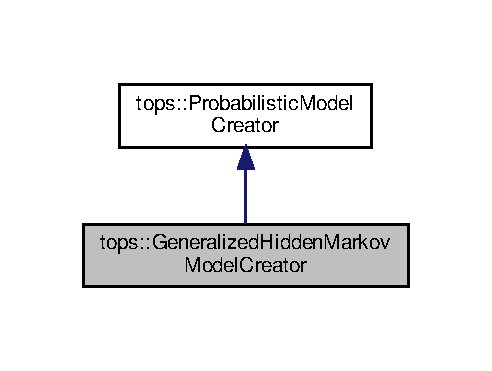
\includegraphics[width=236pt]{classtops_1_1GeneralizedHiddenMarkovModelCreator__inherit__graph}
\end{center}
\end{figure}


Collaboration diagram for tops\+:\+:Generalized\+Hidden\+Markov\+Model\+Creator\+:
\nopagebreak
\begin{figure}[H]
\begin{center}
\leavevmode
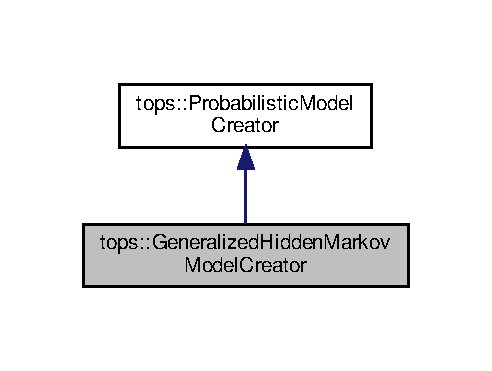
\includegraphics[width=236pt]{classtops_1_1GeneralizedHiddenMarkovModelCreator__coll__graph}
\end{center}
\end{figure}
\subsection*{Public Member Functions}
\begin{DoxyCompactItemize}
\item 
virtual Probabilistic\+Model\+Ptr \hyperlink{classtops_1_1GeneralizedHiddenMarkovModelCreator_a8834cbceabf3922c348c632bb5e660e6}{create} (\hyperlink{classtops_1_1ProbabilisticModelParameters}{Probabilistic\+Model\+Parameters} \&parameters) const
\begin{DoxyCompactList}\small\item\em Creates a probabilistic model. \end{DoxyCompactList}\item 
\mbox{\Hypertarget{classtops_1_1GeneralizedHiddenMarkovModelCreator_a63ce05184acf1030e338198208d470a4}\label{classtops_1_1GeneralizedHiddenMarkovModelCreator_a63ce05184acf1030e338198208d470a4}} 
virtual std\+::string \hyperlink{classtops_1_1GeneralizedHiddenMarkovModelCreator_a63ce05184acf1030e338198208d470a4}{help} () const
\begin{DoxyCompactList}\small\item\em This method returns a help message. \end{DoxyCompactList}\end{DoxyCompactItemize}


\subsection{Detailed Description}
This class is a factory for the finite discrete distribution. 

Definition at line 38 of file Generalized\+Hidden\+Markov\+Model\+Creator.\+hpp.



\subsection{Member Function Documentation}
\mbox{\Hypertarget{classtops_1_1GeneralizedHiddenMarkovModelCreator_a8834cbceabf3922c348c632bb5e660e6}\label{classtops_1_1GeneralizedHiddenMarkovModelCreator_a8834cbceabf3922c348c632bb5e660e6}} 
\index{tops\+::\+Generalized\+Hidden\+Markov\+Model\+Creator@{tops\+::\+Generalized\+Hidden\+Markov\+Model\+Creator}!create@{create}}
\index{create@{create}!tops\+::\+Generalized\+Hidden\+Markov\+Model\+Creator@{tops\+::\+Generalized\+Hidden\+Markov\+Model\+Creator}}
\subsubsection{\texorpdfstring{create()}{create()}}
{\footnotesize\ttfamily Probabilistic\+Model\+Ptr tops\+::\+Generalized\+Hidden\+Markov\+Model\+Creator\+::create (\begin{DoxyParamCaption}\item[{\hyperlink{classtops_1_1ProbabilisticModelParameters}{Probabilistic\+Model\+Parameters} \&}]{parameters }\end{DoxyParamCaption}) const\hspace{0.3cm}{\ttfamily [virtual]}}



Creates a probabilistic model. 


\begin{DoxyParams}{Parameters}
{\em parameters} & is a set of parameters that is utilized to build the model \\
\hline
\end{DoxyParams}


Reimplemented from \hyperlink{classtops_1_1ProbabilisticModelCreator_afed6c8ffa45fff446bdaa8b533da8f7c}{tops\+::\+Probabilistic\+Model\+Creator}.



Definition at line 38 of file Generalized\+Hidden\+Markov\+Model\+Creator.\+cpp.


\begin{DoxyCode}
39                                                                                                            
                \{
40     ProbabilisticModelParameterValuePtr state\_names\_par =
41       parameters.getMandatoryParameterValue(\textcolor{stringliteral}{"state\_names"});
42     ProbabilisticModelParameterValuePtr initial\_probabilities\_par =
43       parameters.getMandatoryParameterValue(\textcolor{stringliteral}{"initial\_probabilities"});
44     ProbabilisticModelParameterValuePtr transitions\_par =
45       parameters.getMandatoryParameterValue(\textcolor{stringliteral}{"transitions"});
46     ProbabilisticModelParameterValuePtr observation\_symbols\_par =
47       parameters.getMandatoryParameterValue(\textcolor{stringliteral}{"observation\_symbols"});
48 
49     GeneralizedHiddenMarkovModelPtr m = GeneralizedHiddenMarkovModelPtr(
50                                                                         \textcolor{keyword}{new} GeneralizedHiddenMarkovModel())
      ;
51 
52     \textcolor{keywordflow}{if} ((state\_names\_par == NULL) || (initial\_probabilities\_par == NULL)
53         || (transitions\_par == NULL) || (observation\_symbols\_par == NULL)) \{
54       std::cerr << \hyperlink{classtops_1_1GeneralizedHiddenMarkovModelCreator_a63ce05184acf1030e338198208d470a4}{help}() << std::endl;
55       \textcolor{keywordflow}{return} m;
56     \}
57 
58     m->initialize(parameters);
59     \textcolor{keywordflow}{return} m;
60 
61   \}
\end{DoxyCode}


The documentation for this class was generated from the following files\+:\begin{DoxyCompactItemize}
\item 
src/Generalized\+Hidden\+Markov\+Model\+Creator.\+hpp\item 
src/Generalized\+Hidden\+Markov\+Model\+Creator.\+cpp\end{DoxyCompactItemize}

\hypertarget{classtops_1_1GeneralizedPairHiddenMarkovModel}{}\section{tops\+:\+:Generalized\+Pair\+Hidden\+Markov\+Model Class Reference}
\label{classtops_1_1GeneralizedPairHiddenMarkovModel}\index{tops\+::\+Generalized\+Pair\+Hidden\+Markov\+Model@{tops\+::\+Generalized\+Pair\+Hidden\+Markov\+Model}}


Inheritance diagram for tops\+:\+:Generalized\+Pair\+Hidden\+Markov\+Model\+:
\nopagebreak
\begin{figure}[H]
\begin{center}
\leavevmode
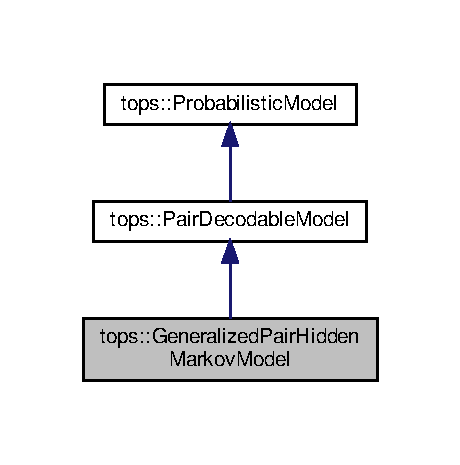
\includegraphics[width=221pt]{classtops_1_1GeneralizedPairHiddenMarkovModel__inherit__graph}
\end{center}
\end{figure}


Collaboration diagram for tops\+:\+:Generalized\+Pair\+Hidden\+Markov\+Model\+:
\nopagebreak
\begin{figure}[H]
\begin{center}
\leavevmode
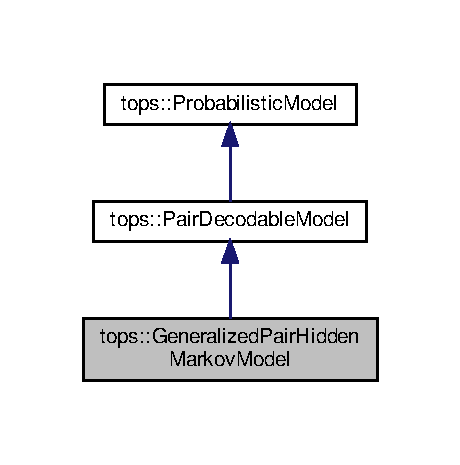
\includegraphics[width=221pt]{classtops_1_1GeneralizedPairHiddenMarkovModel__coll__graph}
\end{center}
\end{figure}
\subsection*{Public Member Functions}
\begin{DoxyCompactItemize}
\item 
\mbox{\Hypertarget{classtops_1_1GeneralizedPairHiddenMarkovModel_a7419fbad2199f504b84f492be603281a}\label{classtops_1_1GeneralizedPairHiddenMarkovModel_a7419fbad2199f504b84f492be603281a}} 
virtual void {\bfseries initialize} (const \hyperlink{classtops_1_1ProbabilisticModelParameters}{Probabilistic\+Model\+Parameters} \&par)
\item 
\mbox{\Hypertarget{classtops_1_1GeneralizedPairHiddenMarkovModel_a1f5984bf7b929bf2619c93a01e7d582e}\label{classtops_1_1GeneralizedPairHiddenMarkovModel_a1f5984bf7b929bf2619c93a01e7d582e}} 
virtual std\+::string \hyperlink{classtops_1_1GeneralizedPairHiddenMarkovModel_a1f5984bf7b929bf2619c93a01e7d582e}{model\+\_\+name} () const
\begin{DoxyCompactList}\small\item\em returns the model name \end{DoxyCompactList}\item 
\mbox{\Hypertarget{classtops_1_1GeneralizedPairHiddenMarkovModel_ae059692ad74c1052d4e7b3eaa3a4f17d}\label{classtops_1_1GeneralizedPairHiddenMarkovModel_ae059692ad74c1052d4e7b3eaa3a4f17d}} 
virtual \hyperlink{classtops_1_1PairDecodableModel}{Pair\+Decodable\+Model} $\ast$ {\bfseries pair\+Decodable} ()
\item 
\mbox{\Hypertarget{classtops_1_1GeneralizedPairHiddenMarkovModel_a04f95a6d9a7a7117623a4e2d0843b663}\label{classtops_1_1GeneralizedPairHiddenMarkovModel_a04f95a6d9a7a7117623a4e2d0843b663}} 
void {\bfseries set\+Initial\+Probabilities} (Discrete\+I\+I\+D\+Model\+Ptr init)
\item 
\mbox{\Hypertarget{classtops_1_1GeneralizedPairHiddenMarkovModel_a11a0385fdc0a6193f171da0c14143556}\label{classtops_1_1GeneralizedPairHiddenMarkovModel_a11a0385fdc0a6193f171da0c14143556}} 
Discrete\+I\+I\+D\+Model\+Ptr {\bfseries initial\+Probabilities} ()
\item 
\mbox{\Hypertarget{classtops_1_1GeneralizedPairHiddenMarkovModel_a012f49565891748243f04d3ee60bfad4}\label{classtops_1_1GeneralizedPairHiddenMarkovModel_a012f49565891748243f04d3ee60bfad4}} 
double {\bfseries forward} (const Sequence \&seq1, const Sequence \&seq2, vector$<$ Matrix $>$ \&a)
\item 
\mbox{\Hypertarget{classtops_1_1GeneralizedPairHiddenMarkovModel_a5f0fe994bb25852ea65d2f0b547918d1}\label{classtops_1_1GeneralizedPairHiddenMarkovModel_a5f0fe994bb25852ea65d2f0b547918d1}} 
virtual double {\bfseries backward} (const Sequence \&seq1, const Sequence \&seq2, vector$<$ Matrix $>$ \&a)
\item 
\mbox{\Hypertarget{classtops_1_1GeneralizedPairHiddenMarkovModel_aa472191f618dded4021c29997e9aaa43}\label{classtops_1_1GeneralizedPairHiddenMarkovModel_aa472191f618dded4021c29997e9aaa43}} 
virtual double {\bfseries viterbi} (const Sequence \&seq1, const Sequence \&seq2, Sequence \&path, Sequence \&al1, Sequence \&al2, vector$<$ Matrix $>$ \&a)
\end{DoxyCompactItemize}
\subsection*{Additional Inherited Members}


\subsection{Detailed Description}


Definition at line 88 of file Generalized\+Pair\+Hidden\+Markov\+Model.\+hpp.



The documentation for this class was generated from the following files\+:\begin{DoxyCompactItemize}
\item 
src/Generalized\+Pair\+Hidden\+Markov\+Model.\+hpp\item 
src/Generalized\+Pair\+Hidden\+Markov\+Model.\+cpp\end{DoxyCompactItemize}

\hypertarget{classtops_1_1GeneralizedPairHiddenMarkovModelCreator}{}\section{tops\+:\+:Generalized\+Pair\+Hidden\+Markov\+Model\+Creator Class Reference}
\label{classtops_1_1GeneralizedPairHiddenMarkovModelCreator}\index{tops\+::\+Generalized\+Pair\+Hidden\+Markov\+Model\+Creator@{tops\+::\+Generalized\+Pair\+Hidden\+Markov\+Model\+Creator}}


Inheritance diagram for tops\+:\+:Generalized\+Pair\+Hidden\+Markov\+Model\+Creator\+:
\nopagebreak
\begin{figure}[H]
\begin{center}
\leavevmode
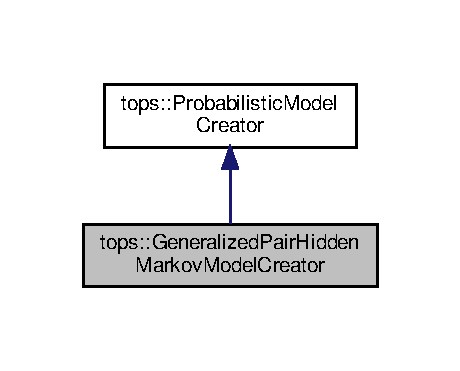
\includegraphics[width=221pt]{classtops_1_1GeneralizedPairHiddenMarkovModelCreator__inherit__graph}
\end{center}
\end{figure}


Collaboration diagram for tops\+:\+:Generalized\+Pair\+Hidden\+Markov\+Model\+Creator\+:
\nopagebreak
\begin{figure}[H]
\begin{center}
\leavevmode
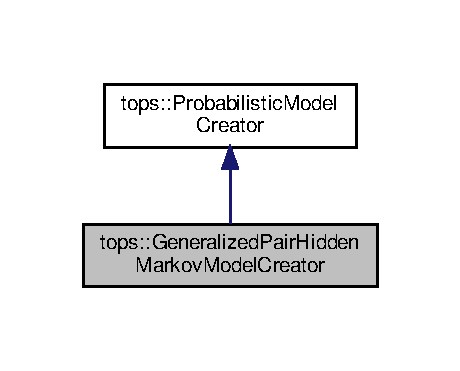
\includegraphics[width=221pt]{classtops_1_1GeneralizedPairHiddenMarkovModelCreator__coll__graph}
\end{center}
\end{figure}
\subsection*{Public Member Functions}
\begin{DoxyCompactItemize}
\item 
virtual Probabilistic\+Model\+Ptr \hyperlink{classtops_1_1GeneralizedPairHiddenMarkovModelCreator_a0f83a29fb5bf772d82ce311ba3e16216}{create} (\hyperlink{classtops_1_1ProbabilisticModelParameters}{Probabilistic\+Model\+Parameters} \&parameters) const
\begin{DoxyCompactList}\small\item\em Creates a probabilistic model. \end{DoxyCompactList}\item 
\mbox{\Hypertarget{classtops_1_1GeneralizedPairHiddenMarkovModelCreator_a51574d0c38fdf8b8fd2d703b4481b861}\label{classtops_1_1GeneralizedPairHiddenMarkovModelCreator_a51574d0c38fdf8b8fd2d703b4481b861}} 
virtual std\+::string \hyperlink{classtops_1_1GeneralizedPairHiddenMarkovModelCreator_a51574d0c38fdf8b8fd2d703b4481b861}{help} () const
\begin{DoxyCompactList}\small\item\em This method returns a help message. \end{DoxyCompactList}\end{DoxyCompactItemize}


\subsection{Detailed Description}


Definition at line 9 of file Generalized\+Pair\+Hidden\+Markov\+Model\+Creator.\+hpp.



\subsection{Member Function Documentation}
\mbox{\Hypertarget{classtops_1_1GeneralizedPairHiddenMarkovModelCreator_a0f83a29fb5bf772d82ce311ba3e16216}\label{classtops_1_1GeneralizedPairHiddenMarkovModelCreator_a0f83a29fb5bf772d82ce311ba3e16216}} 
\index{tops\+::\+Generalized\+Pair\+Hidden\+Markov\+Model\+Creator@{tops\+::\+Generalized\+Pair\+Hidden\+Markov\+Model\+Creator}!create@{create}}
\index{create@{create}!tops\+::\+Generalized\+Pair\+Hidden\+Markov\+Model\+Creator@{tops\+::\+Generalized\+Pair\+Hidden\+Markov\+Model\+Creator}}
\subsubsection{\texorpdfstring{create()}{create()}}
{\footnotesize\ttfamily Probabilistic\+Model\+Ptr tops\+::\+Generalized\+Pair\+Hidden\+Markov\+Model\+Creator\+::create (\begin{DoxyParamCaption}\item[{\hyperlink{classtops_1_1ProbabilisticModelParameters}{Probabilistic\+Model\+Parameters} \&}]{parameters }\end{DoxyParamCaption}) const\hspace{0.3cm}{\ttfamily [virtual]}}



Creates a probabilistic model. 


\begin{DoxyParams}{Parameters}
{\em parameters} & is a set of parameters that is utilized to build the model \\
\hline
\end{DoxyParams}


Reimplemented from \hyperlink{classtops_1_1ProbabilisticModelCreator_afed6c8ffa45fff446bdaa8b533da8f7c}{tops\+::\+Probabilistic\+Model\+Creator}.



Definition at line 6 of file Generalized\+Pair\+Hidden\+Markov\+Model\+Creator.\+cpp.


\begin{DoxyCode}
6                                                                                                            
                  \{
7     ProbabilisticModelParameterValuePtr state\_names = parameters.getMandatoryParameterValue(\textcolor{stringliteral}{"state\_names"});
8     ProbabilisticModelParameterValuePtr observation\_symbols = parameters.getMandatoryParameterValue(\textcolor{stringliteral}{"
      observation\_symbols"});
9     ProbabilisticModelParameterValuePtr number\_of\_emissions = parameters.getMandatoryParameterValue(\textcolor{stringliteral}{"
      number\_of\_emissions"});
10     ProbabilisticModelParameterValuePtr initial\_probabilities = parameters.getMandatoryParameterValue(\textcolor{stringliteral}{"
      initial\_probabilities"});   
11     ProbabilisticModelParameterValuePtr end\_probabilities = parameters.getMandatoryParameterValue(\textcolor{stringliteral}{"
      end\_probabilities"});   
12     ProbabilisticModelParameterValuePtr transitions = parameters.getMandatoryParameterValue(\textcolor{stringliteral}{"transitions"});
13     ProbabilisticModelParameterValuePtr emissions = parameters.getMandatoryParameterValue(\textcolor{stringliteral}{"
      emission\_probabilities"});
14     ProbabilisticModelParameterValuePtr durations = parameters.getOptionalParameterValue(\textcolor{stringliteral}{"
      duration\_probabilities"});
15 
16     \textcolor{keywordflow}{if}((state\_names == NULL)||
17        (observation\_symbols == NULL)||
18        (number\_of\_emissions == NULL) || 
19        (initial\_probabilities == NULL) || 
20        (end\_probabilities == NULL) || 
21        (transitions == NULL) || 
22        (emissions == NULL)) 
23       \{
24     std::cerr << \hyperlink{classtops_1_1GeneralizedPairHiddenMarkovModelCreator_a51574d0c38fdf8b8fd2d703b4481b861}{help}() << std::endl;
25       \}
26     ProbabilisticModelPtr model = GeneralizedPairHiddenMarkovModelPtr(\textcolor{keyword}{new} GeneralizedPairHiddenMarkovModel(
      ));
27     model->initialize(parameters);
28     \textcolor{keywordflow}{return} model;
29   \}
\end{DoxyCode}


The documentation for this class was generated from the following files\+:\begin{DoxyCompactItemize}
\item 
src/Generalized\+Pair\+Hidden\+Markov\+Model\+Creator.\+hpp\item 
src/Generalized\+Pair\+Hidden\+Markov\+Model\+Creator.\+cpp\end{DoxyCompactItemize}

\hypertarget{classtops_1_1GHMMExplicitDurationState}{}\section{tops\+:\+:G\+H\+M\+M\+Explicit\+Duration\+State Class Reference}
\label{classtops_1_1GHMMExplicitDurationState}\index{tops\+::\+G\+H\+M\+M\+Explicit\+Duration\+State@{tops\+::\+G\+H\+M\+M\+Explicit\+Duration\+State}}


G\+H\+MM Explicit duration state.  




{\ttfamily \#include $<$G\+H\+M\+M\+States.\+hpp$>$}



Inheritance diagram for tops\+:\+:G\+H\+M\+M\+Explicit\+Duration\+State\+:
\nopagebreak
\begin{figure}[H]
\begin{center}
\leavevmode
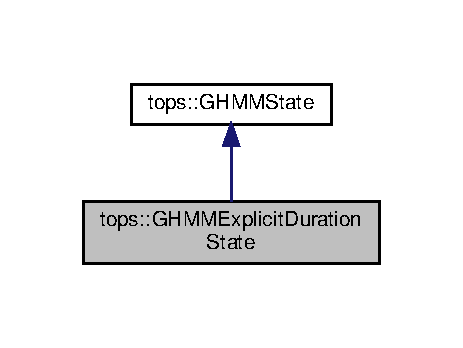
\includegraphics[width=222pt]{classtops_1_1GHMMExplicitDurationState__inherit__graph}
\end{center}
\end{figure}


Collaboration diagram for tops\+:\+:G\+H\+M\+M\+Explicit\+Duration\+State\+:
\nopagebreak
\begin{figure}[H]
\begin{center}
\leavevmode
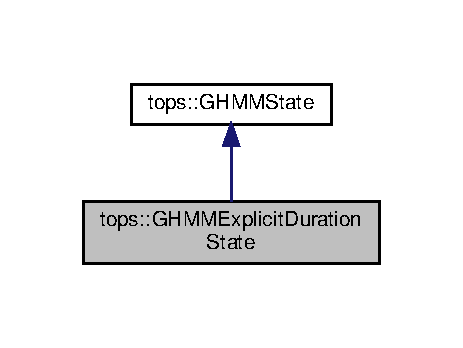
\includegraphics[width=222pt]{classtops_1_1GHMMExplicitDurationState__coll__graph}
\end{center}
\end{figure}
\subsection*{Public Member Functions}
\begin{DoxyCompactItemize}
\item 
\mbox{\Hypertarget{classtops_1_1GHMMExplicitDurationState_acaaab69ef474200c02382e57b8bdb3d4}\label{classtops_1_1GHMMExplicitDurationState_acaaab69ef474200c02382e57b8bdb3d4}} 
{\bfseries G\+H\+M\+M\+Explicit\+Duration\+State} (Probabilistic\+Model\+Ptr observation, Discrete\+I\+I\+D\+Model\+Ptr transition, Symbol\+Ptr name)
\item 
\mbox{\Hypertarget{classtops_1_1GHMMExplicitDurationState_a0da2aed9eb61e299dae400081b9f9a7e}\label{classtops_1_1GHMMExplicitDurationState_a0da2aed9eb61e299dae400081b9f9a7e}} 
virtual void {\bfseries find\+Best\+Predecessor} (Matrix \&gamma, Matrix \&psi, Int\+Matrix \&psilen, const Sequence \&s, int base, const G\+H\+M\+M\+States \&all\+\_\+states, std\+::map$<$ int, std\+::list$<$ int $>$ $>$ \&valid\+\_\+positions)
\item 
\mbox{\Hypertarget{classtops_1_1GHMMExplicitDurationState_a4a14544406eaf4f67715831954351fee}\label{classtops_1_1GHMMExplicitDurationState_a4a14544406eaf4f67715831954351fee}} 
virtual void {\bfseries forward\+Sum} (Matrix \&alpha, const Sequence \&s, int base, const G\+H\+M\+M\+States \&all\+\_\+states, std\+::vector$<$ std\+::list$<$ int $>$ $>$ \&valid\+\_\+positions)
\item 
\mbox{\Hypertarget{classtops_1_1GHMMExplicitDurationState_add57b92313e42bbaa2e95554a695d4f4}\label{classtops_1_1GHMMExplicitDurationState_add57b92313e42bbaa2e95554a695d4f4}} 
virtual double {\bfseries backward\+Sum} (Matrix \&beta, const Sequence \&s, int base, std\+::vector$<$ std\+::list$<$ int $>$ $>$ \&valid\+\_\+positions)
\item 
\mbox{\Hypertarget{classtops_1_1GHMMExplicitDurationState_ae8c44fa2d21d3846feb7aac7186f9192}\label{classtops_1_1GHMMExplicitDurationState_ae8c44fa2d21d3846feb7aac7186f9192}} 
virtual void {\bfseries posterior\+Sum} (Matrix \&alpha, Matrix \&beta, f\+Matrix \&post\+Probs, const Sequence \&s, int base, const G\+H\+M\+M\+States \&all\+\_\+states, std\+::vector$<$ std\+::list$<$ int $>$ $>$ \&valid\+\_\+positions, double prob, int state\+Number)
\item 
\mbox{\Hypertarget{classtops_1_1GHMMExplicitDurationState_a04add3cac332dde621b22acd44a42507}\label{classtops_1_1GHMMExplicitDurationState_a04add3cac332dde621b22acd44a42507}} 
virtual void {\bfseries choose\+Predecessor} (Matrix \&alpha, int base, int \&state, int \&position, const G\+H\+M\+M\+States \&all\+\_\+states)
\item 
\mbox{\Hypertarget{classtops_1_1GHMMExplicitDurationState_a60dd13ec0578ffac894e680b27f65edc}\label{classtops_1_1GHMMExplicitDurationState_a60dd13ec0578ffac894e680b27f65edc}} 
virtual void {\bfseries set\+Duration} (Probabilistic\+Model\+Ptr d)
\item 
\mbox{\Hypertarget{classtops_1_1GHMMExplicitDurationState_ad445b5122638a134e589549d06bbe696}\label{classtops_1_1GHMMExplicitDurationState_ad445b5122638a134e589549d06bbe696}} 
virtual Probabilistic\+Model\+Ptr {\bfseries duration} () const
\item 
\mbox{\Hypertarget{classtops_1_1GHMMExplicitDurationState_adb7d7b6672a77b003d8e1f9932495ff2}\label{classtops_1_1GHMMExplicitDurationState_adb7d7b6672a77b003d8e1f9932495ff2}} 
virtual int {\bfseries choose\+Duration} () const
\item 
\mbox{\Hypertarget{classtops_1_1GHMMExplicitDurationState_a067bee304527756c03bfc4b7491eb25c}\label{classtops_1_1GHMMExplicitDurationState_a067bee304527756c03bfc4b7491eb25c}} 
virtual bool {\bfseries is\+Geometric\+Duration} () const
\item 
\mbox{\Hypertarget{classtops_1_1GHMMExplicitDurationState_a202a6102d036b92a9c872c7ddeae0156}\label{classtops_1_1GHMMExplicitDurationState_a202a6102d036b92a9c872c7ddeae0156}} 
virtual double {\bfseries duration\+\_\+probability} (int l) const
\item 
\mbox{\Hypertarget{classtops_1_1GHMMExplicitDurationState_a5118ccadbebfb98b74975d5ec7fb48d6}\label{classtops_1_1GHMMExplicitDurationState_a5118ccadbebfb98b74975d5ec7fb48d6}} 
virtual std\+::string {\bfseries str} () const
\item 
\mbox{\Hypertarget{classtops_1_1GHMMExplicitDurationState_ae45559048fc040dcaa022d495f0f01bc}\label{classtops_1_1GHMMExplicitDurationState_ae45559048fc040dcaa022d495f0f01bc}} 
virtual void {\bfseries duration\+Model\+Name} (std\+::string name)
\item 
\mbox{\Hypertarget{classtops_1_1GHMMExplicitDurationState_ae3bd1e5677c8c2781e2efd9a47dcb98c}\label{classtops_1_1GHMMExplicitDurationState_ae3bd1e5677c8c2781e2efd9a47dcb98c}} 
virtual std\+::string {\bfseries duration\+Model\+Name} () const
\item 
\mbox{\Hypertarget{classtops_1_1GHMMExplicitDurationState_a6c164e19ae59980a7122de0126840f84}\label{classtops_1_1GHMMExplicitDurationState_a6c164e19ae59980a7122de0126840f84}} 
virtual void {\bfseries fix\+Transition\+Distribution} () const
\item 
\mbox{\Hypertarget{classtops_1_1GHMMExplicitDurationState_ad0999ee0586318ae9076875421744acc}\label{classtops_1_1GHMMExplicitDurationState_ad0999ee0586318ae9076875421744acc}} 
virtual \hyperlink{classtops_1_1ProbabilisticModelParameters}{Probabilistic\+Model\+Parameters} {\bfseries parameters} () const
\end{DoxyCompactItemize}
\subsection*{Additional Inherited Members}


\subsection{Detailed Description}
G\+H\+MM Explicit duration state. 

Definition at line 156 of file G\+H\+M\+M\+States.\+hpp.



The documentation for this class was generated from the following files\+:\begin{DoxyCompactItemize}
\item 
src/G\+H\+M\+M\+States.\+hpp\item 
src/G\+H\+M\+M\+States.\+cpp\end{DoxyCompactItemize}

\hypertarget{classtops_1_1GHMMSignalState}{}\section{tops\+:\+:G\+H\+M\+M\+Signal\+State Class Reference}
\label{classtops_1_1GHMMSignalState}\index{tops\+::\+G\+H\+M\+M\+Signal\+State@{tops\+::\+G\+H\+M\+M\+Signal\+State}}


G\+H\+MM signal states.  




{\ttfamily \#include $<$G\+H\+M\+M\+States.\+hpp$>$}



Inheritance diagram for tops\+:\+:G\+H\+M\+M\+Signal\+State\+:
\nopagebreak
\begin{figure}[H]
\begin{center}
\leavevmode
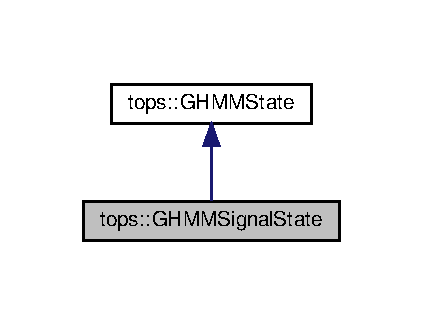
\includegraphics[width=203pt]{classtops_1_1GHMMSignalState__inherit__graph}
\end{center}
\end{figure}


Collaboration diagram for tops\+:\+:G\+H\+M\+M\+Signal\+State\+:
\nopagebreak
\begin{figure}[H]
\begin{center}
\leavevmode
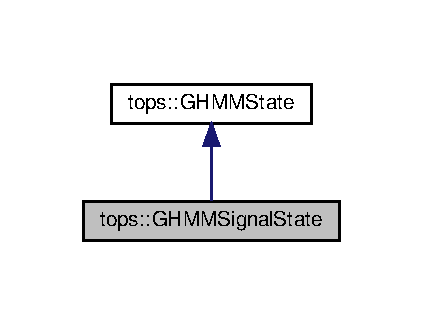
\includegraphics[width=203pt]{classtops_1_1GHMMSignalState__coll__graph}
\end{center}
\end{figure}
\subsection*{Public Member Functions}
\begin{DoxyCompactItemize}
\item 
\mbox{\Hypertarget{classtops_1_1GHMMSignalState_aea28862a4fc11c36188b61cbcfc73916}\label{classtops_1_1GHMMSignalState_aea28862a4fc11c36188b61cbcfc73916}} 
{\bfseries G\+H\+M\+M\+Signal\+State} (Probabilistic\+Model\+Ptr observation, Discrete\+I\+I\+D\+Model\+Ptr transition, Symbol\+Ptr name)
\item 
\mbox{\Hypertarget{classtops_1_1GHMMSignalState_abcaefd7fb338d7ac5f0a264b1c50664a}\label{classtops_1_1GHMMSignalState_abcaefd7fb338d7ac5f0a264b1c50664a}} 
virtual int {\bfseries size} () const
\item 
\mbox{\Hypertarget{classtops_1_1GHMMSignalState_a5d8c08429ffe7b03e2ac715c21ede1ab}\label{classtops_1_1GHMMSignalState_a5d8c08429ffe7b03e2ac715c21ede1ab}} 
virtual void {\bfseries set\+Size} (int s)
\item 
\mbox{\Hypertarget{classtops_1_1GHMMSignalState_a2149cfb9264dc36b7146445d3940cf1d}\label{classtops_1_1GHMMSignalState_a2149cfb9264dc36b7146445d3940cf1d}} 
virtual int {\bfseries choose\+Duration} () const
\item 
\mbox{\Hypertarget{classtops_1_1GHMMSignalState_a53e4742911bd19ec76a6c97df9fb626c}\label{classtops_1_1GHMMSignalState_a53e4742911bd19ec76a6c97df9fb626c}} 
virtual double {\bfseries get\+Threshold} () const
\item 
\mbox{\Hypertarget{classtops_1_1GHMMSignalState_afefd69d7735606350ebe38d6788f55ce}\label{classtops_1_1GHMMSignalState_afefd69d7735606350ebe38d6788f55ce}} 
virtual void {\bfseries set\+Threshold} (double threshold)
\item 
\mbox{\Hypertarget{classtops_1_1GHMMSignalState_a2d80f5ff151a322d2058bdb2fbcc00cc}\label{classtops_1_1GHMMSignalState_a2d80f5ff151a322d2058bdb2fbcc00cc}} 
virtual double {\bfseries duration\+\_\+probability} (int l) const
\item 
\mbox{\Hypertarget{classtops_1_1GHMMSignalState_a8f5bb288a212046737605d074ce61c88}\label{classtops_1_1GHMMSignalState_a8f5bb288a212046737605d074ce61c88}} 
virtual std\+::string {\bfseries str} () const
\item 
\mbox{\Hypertarget{classtops_1_1GHMMSignalState_a414fe1dda478ffedddacf745ddfc6985}\label{classtops_1_1GHMMSignalState_a414fe1dda478ffedddacf745ddfc6985}} 
virtual bool {\bfseries is\+Geometric\+Duration} () const
\item 
\mbox{\Hypertarget{classtops_1_1GHMMSignalState_a43a5c14c3c5a5e2278e86eac5342eb92}\label{classtops_1_1GHMMSignalState_a43a5c14c3c5a5e2278e86eac5342eb92}} 
virtual \hyperlink{classtops_1_1ProbabilisticModelParameters}{Probabilistic\+Model\+Parameters} {\bfseries parameters} () const
\item 
\mbox{\Hypertarget{classtops_1_1GHMMSignalState_afdea9614f4a1ba184c1b51a38e4f0d7b}\label{classtops_1_1GHMMSignalState_afdea9614f4a1ba184c1b51a38e4f0d7b}} 
virtual void {\bfseries fix\+Transition\+Distribution} () const
\item 
\mbox{\Hypertarget{classtops_1_1GHMMSignalState_a370aa0c3dcff2ad533d3e0948c4e44e1}\label{classtops_1_1GHMMSignalState_a370aa0c3dcff2ad533d3e0948c4e44e1}} 
virtual void {\bfseries find\+Best\+Predecessor} (Matrix \&gamma, Matrix \&psi, Int\+Matrix \&psilen, const Sequence \&s, int base, const G\+H\+M\+M\+States \&all\+\_\+states, std\+::map$<$ int, std\+::list$<$ int $>$ $>$ \&valid\+\_\+positions)
\item 
\mbox{\Hypertarget{classtops_1_1GHMMSignalState_ab2d59a2b4f8f7acf7dce68735f279e16}\label{classtops_1_1GHMMSignalState_ab2d59a2b4f8f7acf7dce68735f279e16}} 
virtual void {\bfseries forward\+Sum} (Matrix \&alpha, const Sequence \&s, int base, const G\+H\+M\+M\+States \&all\+\_\+states, std\+::vector$<$ std\+::list$<$ int $>$ $>$ \&valid\+\_\+positions)
\item 
\mbox{\Hypertarget{classtops_1_1GHMMSignalState_ab62dc024ea9a723561d7c25e7d65eda2}\label{classtops_1_1GHMMSignalState_ab62dc024ea9a723561d7c25e7d65eda2}} 
virtual double {\bfseries backward\+Sum} (Matrix \&beta, const Sequence \&s, int base, std\+::vector$<$ std\+::list$<$ int $>$ $>$ \&valid\+\_\+positions)
\item 
\mbox{\Hypertarget{classtops_1_1GHMMSignalState_ac8fad3365487d4be9bf7c0015f4d4cc2}\label{classtops_1_1GHMMSignalState_ac8fad3365487d4be9bf7c0015f4d4cc2}} 
virtual void {\bfseries posterior\+Sum} (Matrix \&alpha, Matrix \&beta, f\+Matrix \&post\+Probs, const Sequence \&s, int base, const G\+H\+M\+M\+States \&all\+\_\+states, std\+::vector$<$ std\+::list$<$ int $>$ $>$ \&valid\+\_\+positions, double prob, int state\+Number)
\item 
\mbox{\Hypertarget{classtops_1_1GHMMSignalState_adc33b138f58cb0fc4ca6d2986e83a839}\label{classtops_1_1GHMMSignalState_adc33b138f58cb0fc4ca6d2986e83a839}} 
virtual void {\bfseries choose\+Predecessor} (Matrix \&alpha, int base, int \&state, int \&position, const G\+H\+M\+M\+States \&all\+\_\+states)
\end{DoxyCompactItemize}
\subsection*{Additional Inherited Members}


\subsection{Detailed Description}
G\+H\+MM signal states. 

Definition at line 125 of file G\+H\+M\+M\+States.\+hpp.



The documentation for this class was generated from the following files\+:\begin{DoxyCompactItemize}
\item 
src/G\+H\+M\+M\+States.\+hpp\item 
src/G\+H\+M\+M\+States.\+cpp\end{DoxyCompactItemize}

\hypertarget{classtops_1_1GHMMState}{}\section{tops\+:\+:G\+H\+M\+M\+State Class Reference}
\label{classtops_1_1GHMMState}\index{tops\+::\+G\+H\+M\+M\+State@{tops\+::\+G\+H\+M\+M\+State}}


Represents a G\+H\+MM State.  




{\ttfamily \#include $<$G\+H\+M\+M\+States.\+hpp$>$}



Inheritance diagram for tops\+:\+:G\+H\+M\+M\+State\+:
\nopagebreak
\begin{figure}[H]
\begin{center}
\leavevmode
\includegraphics[width=350pt]{classtops_1_1GHMMState__inherit__graph}
\end{center}
\end{figure}
\subsection*{Public Member Functions}
\begin{DoxyCompactItemize}
\item 
\mbox{\Hypertarget{classtops_1_1GHMMState_a1cb3d607867c47639e56914585624603}\label{classtops_1_1GHMMState_a1cb3d607867c47639e56914585624603}} 
{\bfseries G\+H\+M\+M\+State} (Probabilistic\+Model\+Ptr observation, Discrete\+I\+I\+D\+Model\+Ptr transition, Symbol\+Ptr name)
\item 
\mbox{\Hypertarget{classtops_1_1GHMMState_a5cffd17806bb68c56beb37e8553b5bcd}\label{classtops_1_1GHMMState_a5cffd17806bb68c56beb37e8553b5bcd}} 
virtual void {\bfseries set\+Observation} (Probabilistic\+Model\+Ptr obs)
\item 
\mbox{\Hypertarget{classtops_1_1GHMMState_a173d2e0140e60128e1ef3b9186f1185d}\label{classtops_1_1GHMMState_a173d2e0140e60128e1ef3b9186f1185d}} 
virtual Probabilistic\+Model\+Ptr {\bfseries observation} () const
\item 
\mbox{\Hypertarget{classtops_1_1GHMMState_a49a48dd47af91147ff930fa55f656e38}\label{classtops_1_1GHMMState_a49a48dd47af91147ff930fa55f656e38}} 
virtual void {\bfseries set\+Transition} (Discrete\+I\+I\+D\+Model\+Ptr trans)
\item 
\mbox{\Hypertarget{classtops_1_1GHMMState_a9890351fbd3f312e9be769e324dd274f}\label{classtops_1_1GHMMState_a9890351fbd3f312e9be769e324dd274f}} 
virtual Discrete\+I\+I\+D\+Model\+Ptr {\bfseries transition} () const
\item 
\mbox{\Hypertarget{classtops_1_1GHMMState_a73b2789f91f5631ad64bf80d1a354460}\label{classtops_1_1GHMMState_a73b2789f91f5631ad64bf80d1a354460}} 
virtual int {\bfseries choose\+Duration} () const
\item 
\mbox{\Hypertarget{classtops_1_1GHMMState_a6bd6141cf6f2eaeba1acbaaf84952263}\label{classtops_1_1GHMMState_a6bd6141cf6f2eaeba1acbaaf84952263}} 
virtual std\+::string {\bfseries name} () const
\item 
\mbox{\Hypertarget{classtops_1_1GHMMState_af64f0421ea08e1fe17b485d7de21726b}\label{classtops_1_1GHMMState_af64f0421ea08e1fe17b485d7de21726b}} 
virtual int {\bfseries id} () const
\item 
\mbox{\Hypertarget{classtops_1_1GHMMState_aa0f1cdd4f9f4f54350f6a9fdb1ea6201}\label{classtops_1_1GHMMState_aa0f1cdd4f9f4f54350f6a9fdb1ea6201}} 
virtual void {\bfseries add\+Predecessor} (int id)
\item 
\mbox{\Hypertarget{classtops_1_1GHMMState_a5e429753bcdf0bd8c91e9361ba90e735}\label{classtops_1_1GHMMState_a5e429753bcdf0bd8c91e9361ba90e735}} 
virtual std\+::vector$<$ int $>$ \& {\bfseries predecessors} ()
\item 
\mbox{\Hypertarget{classtops_1_1GHMMState_a7662df37573e3b25f9daadd5e3a643db}\label{classtops_1_1GHMMState_a7662df37573e3b25f9daadd5e3a643db}} 
virtual void {\bfseries add\+Successor} (int id)
\item 
\mbox{\Hypertarget{classtops_1_1GHMMState_af08bcd3ee8206343f63e99cf78f94164}\label{classtops_1_1GHMMState_af08bcd3ee8206343f63e99cf78f94164}} 
virtual void {\bfseries clear\+Predecessor\+Successor} ()
\item 
\mbox{\Hypertarget{classtops_1_1GHMMState_a3da3b418c150ee4eae8d747ea557604c}\label{classtops_1_1GHMMState_a3da3b418c150ee4eae8d747ea557604c}} 
virtual std\+::vector$<$ int $>$ \& {\bfseries successors} ()
\item 
\mbox{\Hypertarget{classtops_1_1GHMMState_a538396303b95638b3de6b5a32b5fb644}\label{classtops_1_1GHMMState_a538396303b95638b3de6b5a32b5fb644}} 
virtual std\+::vector$<$ int $>$ \& {\bfseries classes} ()
\item 
\mbox{\Hypertarget{classtops_1_1GHMMState_a258eeab65d4ce831171fb3ef56eff353}\label{classtops_1_1GHMMState_a258eeab65d4ce831171fb3ef56eff353}} 
virtual void {\bfseries set\+Classes} (std\+::vector$<$ int $>$ \&classes)
\item 
\mbox{\Hypertarget{classtops_1_1GHMMState_a2fad943358b1b695c4a7499522d61823}\label{classtops_1_1GHMMState_a2fad943358b1b695c4a7499522d61823}} 
virtual double {\bfseries duration\+\_\+probability} (int l) const
\item 
\mbox{\Hypertarget{classtops_1_1GHMMState_af96504cfe3967a72b85cea606e0988b6}\label{classtops_1_1GHMMState_af96504cfe3967a72b85cea606e0988b6}} 
virtual bool {\bfseries is\+Geometric\+Duration} () const
\item 
\mbox{\Hypertarget{classtops_1_1GHMMState_a7eb198f5d1460825cf3fd59f987a3440}\label{classtops_1_1GHMMState_a7eb198f5d1460825cf3fd59f987a3440}} 
virtual std\+::string {\bfseries str} () const
\item 
\mbox{\Hypertarget{classtops_1_1GHMMState_aff00289974baefc3dad3ca95b50669ba}\label{classtops_1_1GHMMState_aff00289974baefc3dad3ca95b50669ba}} 
virtual int {\bfseries get\+Input\+Phase} () const
\item 
\mbox{\Hypertarget{classtops_1_1GHMMState_a6bc36d68a563b01db5569a101f1a750a}\label{classtops_1_1GHMMState_a6bc36d68a563b01db5569a101f1a750a}} 
virtual void {\bfseries set\+Input\+Phase} (int \+\_\+input\+Phase)
\item 
\mbox{\Hypertarget{classtops_1_1GHMMState_ae265b35c0f29e8f9e5dc26c20490643e}\label{classtops_1_1GHMMState_ae265b35c0f29e8f9e5dc26c20490643e}} 
virtual int {\bfseries get\+Output\+Phase} () const
\item 
\mbox{\Hypertarget{classtops_1_1GHMMState_a83310d7c4cafe023ae12ea7e8ec52a4f}\label{classtops_1_1GHMMState_a83310d7c4cafe023ae12ea7e8ec52a4f}} 
virtual void {\bfseries set\+Output\+Phase} (int \+\_\+output\+Phase)
\item 
\mbox{\Hypertarget{classtops_1_1GHMMState_a88c726adf531df277ee23ed3bdecdabe}\label{classtops_1_1GHMMState_a88c726adf531df277ee23ed3bdecdabe}} 
virtual int {\bfseries get\+Start} () const
\item 
\mbox{\Hypertarget{classtops_1_1GHMMState_a3fc74623c2cafc82390619508998fd60}\label{classtops_1_1GHMMState_a3fc74623c2cafc82390619508998fd60}} 
virtual void {\bfseries set\+Start} (int start)
\item 
\mbox{\Hypertarget{classtops_1_1GHMMState_ac50009adb860a78432ed14fb1f83ba60}\label{classtops_1_1GHMMState_ac50009adb860a78432ed14fb1f83ba60}} 
virtual int {\bfseries get\+Stop} () const
\item 
\mbox{\Hypertarget{classtops_1_1GHMMState_a16e51ba0cf3426ac5de1c739fcd1f3f6}\label{classtops_1_1GHMMState_a16e51ba0cf3426ac5de1c739fcd1f3f6}} 
virtual void {\bfseries set\+Stop} (int stop)
\item 
\mbox{\Hypertarget{classtops_1_1GHMMState_aba4facd57e95105b2f997082befd672b}\label{classtops_1_1GHMMState_aba4facd57e95105b2f997082befd672b}} 
virtual void {\bfseries is\+Left\+Joinable} (int joinable)
\item 
\mbox{\Hypertarget{classtops_1_1GHMMState_a428a59b0f6958382d34b1e6323b2aa8e}\label{classtops_1_1GHMMState_a428a59b0f6958382d34b1e6323b2aa8e}} 
virtual int {\bfseries is\+Left\+Joinable} () const
\item 
\mbox{\Hypertarget{classtops_1_1GHMMState_a6b3ecb6bd87412895604c7f8cda87d10}\label{classtops_1_1GHMMState_a6b3ecb6bd87412895604c7f8cda87d10}} 
virtual void {\bfseries is\+Right\+Joinable} (int joinable)
\item 
\mbox{\Hypertarget{classtops_1_1GHMMState_a9686860dee6c78bcb24c5b61214a8bec}\label{classtops_1_1GHMMState_a9686860dee6c78bcb24c5b61214a8bec}} 
virtual int {\bfseries is\+Right\+Joinable} () const
\item 
\mbox{\Hypertarget{classtops_1_1GHMMState_ae0545d894a03b676faaf4170af2e4b54}\label{classtops_1_1GHMMState_ae0545d894a03b676faaf4170af2e4b54}} 
virtual void {\bfseries observation\+Model\+Name} (std\+::string name)
\item 
\mbox{\Hypertarget{classtops_1_1GHMMState_a74b5d6f4fc4fc45d102a7f1199c3f147}\label{classtops_1_1GHMMState_a74b5d6f4fc4fc45d102a7f1199c3f147}} 
virtual void {\bfseries duration\+Model\+Name} (std\+::string name)
\item 
\mbox{\Hypertarget{classtops_1_1GHMMState_adf5b5592a4be45f5227932be94d9ec71}\label{classtops_1_1GHMMState_adf5b5592a4be45f5227932be94d9ec71}} 
virtual std\+::string {\bfseries observation\+Model\+Name} () const
\item 
\mbox{\Hypertarget{classtops_1_1GHMMState_a5193759c7ad20b08bda548e208450dae}\label{classtops_1_1GHMMState_a5193759c7ad20b08bda548e208450dae}} 
virtual std\+::string {\bfseries duration\+Model\+Name} () const
\item 
\mbox{\Hypertarget{classtops_1_1GHMMState_a3458044303664790d6b94bedcd93817e}\label{classtops_1_1GHMMState_a3458044303664790d6b94bedcd93817e}} 
virtual void {\bfseries fix\+Transition\+Distribution} () const
\item 
\mbox{\Hypertarget{classtops_1_1GHMMState_ad20832debfe3bdc2b6d596c90f3ebbe6}\label{classtops_1_1GHMMState_ad20832debfe3bdc2b6d596c90f3ebbe6}} 
virtual \hyperlink{classtops_1_1ProbabilisticModelParameters}{Probabilistic\+Model\+Parameters} {\bfseries parameters} () const
\item 
\mbox{\Hypertarget{classtops_1_1GHMMState_a90571a7a103183c61b548ffa5ad6664a}\label{classtops_1_1GHMMState_a90571a7a103183c61b548ffa5ad6664a}} 
virtual void {\bfseries find\+Best\+Predecessor} (Matrix \&gamma, Matrix \&psi, Int\+Matrix \&psilen, const Sequence \&s, int base, const G\+H\+M\+M\+States \&all\+\_\+states, std\+::map$<$ int, std\+::list$<$ int $>$ $>$ \&valid\+\_\+positions)
\item 
\mbox{\Hypertarget{classtops_1_1GHMMState_a5f3bbebf623a5b8d7bcbdae77f9ff3b8}\label{classtops_1_1GHMMState_a5f3bbebf623a5b8d7bcbdae77f9ff3b8}} 
virtual void {\bfseries forward\+Sum} (Matrix \&alpha, const Sequence \&s, int base, const G\+H\+M\+M\+States \&all\+\_\+states, std\+::vector$<$ std\+::list$<$ int $>$ $>$ \&valid\+\_\+positions)
\item 
\mbox{\Hypertarget{classtops_1_1GHMMState_a99ddf156640eee462b671403df991db0}\label{classtops_1_1GHMMState_a99ddf156640eee462b671403df991db0}} 
virtual double {\bfseries backward\+Sum} (Matrix \&beta, const Sequence \&s, int base, std\+::vector$<$ std\+::list$<$ int $>$ $>$ \&valid\+\_\+positions)
\item 
\mbox{\Hypertarget{classtops_1_1GHMMState_a78b48b998f0bd5ffc4dd8f5df87c4ff3}\label{classtops_1_1GHMMState_a78b48b998f0bd5ffc4dd8f5df87c4ff3}} 
virtual void {\bfseries posterior\+Sum} (Matrix \&alpha, Matrix \&beta, f\+Matrix \&post\+Probs, const Sequence \&s, int base, const G\+H\+M\+M\+States \&all\+\_\+states, std\+::vector$<$ std\+::list$<$ int $>$ $>$ \&valid\+\_\+positions, double prob, int state\+Number)
\item 
\mbox{\Hypertarget{classtops_1_1GHMMState_ac12a60c18dcd0b173fde9833a3dac96a}\label{classtops_1_1GHMMState_ac12a60c18dcd0b173fde9833a3dac96a}} 
virtual void {\bfseries choose\+Predecessor} (Matrix \&alpha, int base, int \&state, int \&position, const G\+H\+M\+M\+States \&all\+\_\+states)
\end{DoxyCompactItemize}
\subsection*{Protected Attributes}
\begin{DoxyCompactItemize}
\item 
\mbox{\Hypertarget{classtops_1_1GHMMState_a512b76323ad852ef7616bee1375678ec}\label{classtops_1_1GHMMState_a512b76323ad852ef7616bee1375678ec}} 
Probabilistic\+Model\+Ptr {\bfseries \+\_\+observation}
\item 
\mbox{\Hypertarget{classtops_1_1GHMMState_a815932aebe12c59682943754304cdc07}\label{classtops_1_1GHMMState_a815932aebe12c59682943754304cdc07}} 
Discrete\+I\+I\+D\+Model\+Ptr {\bfseries \+\_\+transition}
\item 
\mbox{\Hypertarget{classtops_1_1GHMMState_a4e1c88c494745d40fc83a59795126fe0}\label{classtops_1_1GHMMState_a4e1c88c494745d40fc83a59795126fe0}} 
Symbol\+Ptr {\bfseries \+\_\+name}
\item 
\mbox{\Hypertarget{classtops_1_1GHMMState_aca20bbc5a5886de1ae78fefe31fccd93}\label{classtops_1_1GHMMState_aca20bbc5a5886de1ae78fefe31fccd93}} 
std\+::vector$<$ int $>$ {\bfseries \+\_\+predecessors}
\item 
\mbox{\Hypertarget{classtops_1_1GHMMState_a72621187f503faa9ed1c1ec0a6c65728}\label{classtops_1_1GHMMState_a72621187f503faa9ed1c1ec0a6c65728}} 
std\+::vector$<$ int $>$ {\bfseries \+\_\+successors}
\item 
\mbox{\Hypertarget{classtops_1_1GHMMState_a7ce4fe584be7096e5253947f79ee77bf}\label{classtops_1_1GHMMState_a7ce4fe584be7096e5253947f79ee77bf}} 
std\+::vector$<$ int $>$ {\bfseries \+\_\+classes}
\item 
\mbox{\Hypertarget{classtops_1_1GHMMState_ad75b5b9f8ad5798502bf0bc829c99417}\label{classtops_1_1GHMMState_ad75b5b9f8ad5798502bf0bc829c99417}} 
int {\bfseries \+\_\+input\+Phase}
\item 
\mbox{\Hypertarget{classtops_1_1GHMMState_a3ae936eefb22511d727bdea109395eff}\label{classtops_1_1GHMMState_a3ae936eefb22511d727bdea109395eff}} 
int {\bfseries \+\_\+output\+Phase}
\item 
\mbox{\Hypertarget{classtops_1_1GHMMState_a81ae486f388a02ee3a0314aeb07d7f6d}\label{classtops_1_1GHMMState_a81ae486f388a02ee3a0314aeb07d7f6d}} 
int {\bfseries \+\_\+start}
\item 
\mbox{\Hypertarget{classtops_1_1GHMMState_a805e7a977230e52923e02216b4b6ef24}\label{classtops_1_1GHMMState_a805e7a977230e52923e02216b4b6ef24}} 
int {\bfseries \+\_\+stop}
\item 
\mbox{\Hypertarget{classtops_1_1GHMMState_adcfc81f47c0eff0aafc594116b8a715b}\label{classtops_1_1GHMMState_adcfc81f47c0eff0aafc594116b8a715b}} 
bool {\bfseries \+\_\+left\+\_\+joinable}
\item 
\mbox{\Hypertarget{classtops_1_1GHMMState_afbd53d2ada38b96e3ff071da7c2a7c0b}\label{classtops_1_1GHMMState_afbd53d2ada38b96e3ff071da7c2a7c0b}} 
bool {\bfseries \+\_\+right\+\_\+joinable}
\item 
\mbox{\Hypertarget{classtops_1_1GHMMState_a63e57e38cbe809f071693562d00b3cf0}\label{classtops_1_1GHMMState_a63e57e38cbe809f071693562d00b3cf0}} 
std\+::string {\bfseries \+\_\+observation\+Model\+Name}
\end{DoxyCompactItemize}


\subsection{Detailed Description}
Represents a G\+H\+MM State. 

Definition at line 52 of file G\+H\+M\+M\+States.\+hpp.



The documentation for this class was generated from the following files\+:\begin{DoxyCompactItemize}
\item 
src/G\+H\+M\+M\+States.\+hpp\item 
src/G\+H\+M\+M\+States.\+cpp\end{DoxyCompactItemize}

\hypertarget{classtops_1_1GPHMMState}{}\section{tops\+:\+:G\+P\+H\+M\+M\+State Class Reference}
\label{classtops_1_1GPHMMState}\index{tops\+::\+G\+P\+H\+M\+M\+State@{tops\+::\+G\+P\+H\+M\+M\+State}}


Inheritance diagram for tops\+:\+:G\+P\+H\+M\+M\+State\+:
\nopagebreak
\begin{figure}[H]
\begin{center}
\leavevmode
\includegraphics[width=208pt]{classtops_1_1GPHMMState__inherit__graph}
\end{center}
\end{figure}


Collaboration diagram for tops\+:\+:G\+P\+H\+M\+M\+State\+:
\nopagebreak
\begin{figure}[H]
\begin{center}
\leavevmode
\includegraphics[width=208pt]{classtops_1_1GPHMMState__coll__graph}
\end{center}
\end{figure}
\subsection*{Public Member Functions}
\begin{DoxyCompactItemize}
\item 
\mbox{\Hypertarget{classtops_1_1GPHMMState_a59b8730fbfe7e1b38f4183374d45552b}\label{classtops_1_1GPHMMState_a59b8730fbfe7e1b38f4183374d45552b}} 
{\bfseries G\+P\+H\+M\+M\+State} (int id, Symbol\+Ptr name, Probabilistic\+Model\+Ptr emission, Discrete\+I\+I\+D\+Model\+Ptr transitions, Probabilistic\+Model\+Ptr duration, Int\+Vector i\+Transitions, Int\+Vector o\+Transitions, int max\+Seq1, int min\+Seq1, int max\+Seq2, int min\+Seq2)
\item 
\mbox{\Hypertarget{classtops_1_1GPHMMState_a80f80ccfaf58e48f1047c4cab55b7d64}\label{classtops_1_1GPHMMState_a80f80ccfaf58e48f1047c4cab55b7d64}} 
int {\bfseries max\+Seq1} ()
\item 
\mbox{\Hypertarget{classtops_1_1GPHMMState_a7b93516f9ac6604c2e03a6d59dfa0bb2}\label{classtops_1_1GPHMMState_a7b93516f9ac6604c2e03a6d59dfa0bb2}} 
int {\bfseries min\+Seq1} ()
\item 
\mbox{\Hypertarget{classtops_1_1GPHMMState_a43491b35a646c975207c23d243f507f3}\label{classtops_1_1GPHMMState_a43491b35a646c975207c23d243f507f3}} 
int {\bfseries max\+Seq2} ()
\item 
\mbox{\Hypertarget{classtops_1_1GPHMMState_a2e9ef8d39a98a4dc297bfaf986f20f8a}\label{classtops_1_1GPHMMState_a2e9ef8d39a98a4dc297bfaf986f20f8a}} 
int {\bfseries min\+Seq2} ()
\item 
\mbox{\Hypertarget{classtops_1_1GPHMMState_ad9f417057211aad8ffb00274d342a8ae}\label{classtops_1_1GPHMMState_ad9f417057211aad8ffb00274d342a8ae}} 
Probabilistic\+Model\+Ptr {\bfseries duration} ()
\end{DoxyCompactItemize}
\subsection*{Additional Inherited Members}


\subsection{Detailed Description}


Definition at line 22 of file Generalized\+Pair\+Hidden\+Markov\+Model.\+hpp.



The documentation for this class was generated from the following file\+:\begin{DoxyCompactItemize}
\item 
src/Generalized\+Pair\+Hidden\+Markov\+Model.\+hpp\end{DoxyCompactItemize}

\hypertarget{classtops_1_1HiddenMarkovModel}{}\section{tops\+:\+:Hidden\+Markov\+Model Class Reference}
\label{classtops_1_1HiddenMarkovModel}\index{tops\+::\+Hidden\+Markov\+Model@{tops\+::\+Hidden\+Markov\+Model}}


This class represents a hidden markov model.  




{\ttfamily \#include $<$Hidden\+Markov\+Model.\+hpp$>$}



Inheritance diagram for tops\+:\+:Hidden\+Markov\+Model\+:
\nopagebreak
\begin{figure}[H]
\begin{center}
\leavevmode
\includegraphics[width=211pt]{classtops_1_1HiddenMarkovModel__inherit__graph}
\end{center}
\end{figure}


Collaboration diagram for tops\+:\+:Hidden\+Markov\+Model\+:
\nopagebreak
\begin{figure}[H]
\begin{center}
\leavevmode
\includegraphics[width=211pt]{classtops_1_1HiddenMarkovModel__coll__graph}
\end{center}
\end{figure}
\subsection*{Public Member Functions}
\begin{DoxyCompactItemize}
\item 
\mbox{\Hypertarget{classtops_1_1HiddenMarkovModel_ac0cd3b6db315de5f6dd543db4910d4dc}\label{classtops_1_1HiddenMarkovModel_ac0cd3b6db315de5f6dd543db4910d4dc}} 
{\bfseries Hidden\+Markov\+Model} (std\+::vector$<$ H\+M\+M\+State\+Ptr $>$ states, Discrete\+I\+I\+D\+Model\+Ptr initial\+\_\+probability, Alphabet\+Ptr state\+\_\+names, Alphabet\+Ptr observation\+\_\+symbols)
\item 
\mbox{\Hypertarget{classtops_1_1HiddenMarkovModel_ad879a83a5fb6847a8e30ce00572c5a31}\label{classtops_1_1HiddenMarkovModel_ad879a83a5fb6847a8e30ce00572c5a31}} 
void {\bfseries set\+States} (std\+::vector$<$ H\+M\+M\+State\+Ptr $>$ states)
\item 
\mbox{\Hypertarget{classtops_1_1HiddenMarkovModel_af9085a6ee9df355a207b0090d2eae284}\label{classtops_1_1HiddenMarkovModel_af9085a6ee9df355a207b0090d2eae284}} 
virtual Sequence \& \hyperlink{classtops_1_1HiddenMarkovModel_af9085a6ee9df355a207b0090d2eae284}{choose\+Observation} (Sequence \&h, int i, int state) const
\begin{DoxyCompactList}\small\item\em Choose the observation given a state. \end{DoxyCompactList}\item 
\mbox{\Hypertarget{classtops_1_1HiddenMarkovModel_a026ac17cc9dbf1f03b74703aa9f48651}\label{classtops_1_1HiddenMarkovModel_a026ac17cc9dbf1f03b74703aa9f48651}} 
virtual int \hyperlink{classtops_1_1HiddenMarkovModel_a026ac17cc9dbf1f03b74703aa9f48651}{choose\+State} (int state) const
\begin{DoxyCompactList}\small\item\em Choose a state. \end{DoxyCompactList}\item 
\mbox{\Hypertarget{classtops_1_1HiddenMarkovModel_a823d2b105395e8aea75d52f40bb30d55}\label{classtops_1_1HiddenMarkovModel_a823d2b105395e8aea75d52f40bb30d55}} 
virtual int \hyperlink{classtops_1_1HiddenMarkovModel_a823d2b105395e8aea75d52f40bb30d55}{choose\+First\+State} () const
\begin{DoxyCompactList}\small\item\em Choose first state. \end{DoxyCompactList}\item 
\mbox{\Hypertarget{classtops_1_1HiddenMarkovModel_a97718c6f22b668611692902c561b6fac}\label{classtops_1_1HiddenMarkovModel_a97718c6f22b668611692902c561b6fac}} 
virtual Alphabet\+Ptr \hyperlink{classtops_1_1HiddenMarkovModel_a97718c6f22b668611692902c561b6fac}{get\+State\+Names} () const
\begin{DoxyCompactList}\small\item\em Get the state names. \end{DoxyCompactList}\item 
\mbox{\Hypertarget{classtops_1_1HiddenMarkovModel_aab4bbb731e757d8e5d0cc1e660f45e63}\label{classtops_1_1HiddenMarkovModel_aab4bbb731e757d8e5d0cc1e660f45e63}} 
virtual std\+::string \hyperlink{classtops_1_1HiddenMarkovModel_aab4bbb731e757d8e5d0cc1e660f45e63}{get\+State\+Name} (int state) const
\begin{DoxyCompactList}\small\item\em Get state name. \end{DoxyCompactList}\item 
\mbox{\Hypertarget{classtops_1_1HiddenMarkovModel_a26a70987f5b4b2acd119c01f7e986f6c}\label{classtops_1_1HiddenMarkovModel_a26a70987f5b4b2acd119c01f7e986f6c}} 
virtual std\+::string \hyperlink{classtops_1_1HiddenMarkovModel_a26a70987f5b4b2acd119c01f7e986f6c}{str} () const
\begin{DoxyCompactList}\small\item\em returns the string representation of the model \end{DoxyCompactList}\item 
\mbox{\Hypertarget{classtops_1_1HiddenMarkovModel_ab77bfeacc3fa135abbf82d6f9887607e}\label{classtops_1_1HiddenMarkovModel_ab77bfeacc3fa135abbf82d6f9887607e}} 
virtual void {\bfseries set\+State} (int id, H\+M\+M\+State\+Ptr state)
\item 
\mbox{\Hypertarget{classtops_1_1HiddenMarkovModel_a3b84fee9e3f217c59a721072ab74167f}\label{classtops_1_1HiddenMarkovModel_a3b84fee9e3f217c59a721072ab74167f}} 
virtual H\+M\+M\+State\+Ptr {\bfseries get\+State} (int id) const
\item 
\mbox{\Hypertarget{classtops_1_1HiddenMarkovModel_aea7c39ddeb051ec95cc7c745e719af35}\label{classtops_1_1HiddenMarkovModel_aea7c39ddeb051ec95cc7c745e719af35}} 
virtual double \hyperlink{classtops_1_1HiddenMarkovModel_aea7c39ddeb051ec95cc7c745e719af35}{forward} (const Sequence \&s, Matrix \&alpha) const
\begin{DoxyCompactList}\small\item\em Forward algorithm. \end{DoxyCompactList}\item 
\mbox{\Hypertarget{classtops_1_1HiddenMarkovModel_aaa1cfc9715c087d453985b5c2d3e02af}\label{classtops_1_1HiddenMarkovModel_aaa1cfc9715c087d453985b5c2d3e02af}} 
virtual double \hyperlink{classtops_1_1HiddenMarkovModel_aaa1cfc9715c087d453985b5c2d3e02af}{backward} (const Sequence \&s, Matrix \&beta) const
\begin{DoxyCompactList}\small\item\em Backward algorithm. \end{DoxyCompactList}\item 
\mbox{\Hypertarget{classtops_1_1HiddenMarkovModel_a40eae6b0b0def5afc0c8051db926e6a8}\label{classtops_1_1HiddenMarkovModel_a40eae6b0b0def5afc0c8051db926e6a8}} 
virtual double \hyperlink{classtops_1_1HiddenMarkovModel_a40eae6b0b0def5afc0c8051db926e6a8}{viterbi} (const Sequence \&s, Sequence \&path, Matrix \&gamma) const
\begin{DoxyCompactList}\small\item\em Viterbi algorithm. \end{DoxyCompactList}\item 
\mbox{\Hypertarget{classtops_1_1HiddenMarkovModel_a1c3e76b1359651087a527a56b161969f}\label{classtops_1_1HiddenMarkovModel_a1c3e76b1359651087a527a56b161969f}} 
virtual std\+::string \hyperlink{classtops_1_1HiddenMarkovModel_a1c3e76b1359651087a527a56b161969f}{model\+\_\+name} () const
\begin{DoxyCompactList}\small\item\em returns the model name \end{DoxyCompactList}\item 
\mbox{\Hypertarget{classtops_1_1HiddenMarkovModel_ade43f35f76f240e4672287229f786daa}\label{classtops_1_1HiddenMarkovModel_ade43f35f76f240e4672287229f786daa}} 
virtual Probabilistic\+Model\+Creator\+Ptr {\bfseries get\+Factory} () const
\item 
\mbox{\Hypertarget{classtops_1_1HiddenMarkovModel_a3c359333874ba9716404bffe44848949}\label{classtops_1_1HiddenMarkovModel_a3c359333874ba9716404bffe44848949}} 
virtual \hyperlink{classtops_1_1DecodableModel}{Decodable\+Model} $\ast$ {\bfseries decodable} ()
\item 
\mbox{\Hypertarget{classtops_1_1HiddenMarkovModel_a5fbe607e546d580e9e32ae01b2a07fd0}\label{classtops_1_1HiddenMarkovModel_a5fbe607e546d580e9e32ae01b2a07fd0}} 
virtual void \hyperlink{classtops_1_1HiddenMarkovModel_a5fbe607e546d580e9e32ae01b2a07fd0}{train\+Baum\+Welch} (Sequence\+List \&training\+\_\+set, int maxiterations, double diff)
\begin{DoxyCompactList}\small\item\em Train baum Welch. \end{DoxyCompactList}\item 
\mbox{\Hypertarget{classtops_1_1HiddenMarkovModel_a6c740f4636089a6f00ef7bd2b003776c}\label{classtops_1_1HiddenMarkovModel_a6c740f4636089a6f00ef7bd2b003776c}} 
virtual void {\bfseries initialize} (const \hyperlink{classtops_1_1ProbabilisticModelParameters}{Probabilistic\+Model\+Parameters} \&par)
\item 
\mbox{\Hypertarget{classtops_1_1HiddenMarkovModel_aa1c80eb4146eef79479e17a44080b007}\label{classtops_1_1HiddenMarkovModel_aa1c80eb4146eef79479e17a44080b007}} 
virtual \hyperlink{classtops_1_1ProbabilisticModelParameters}{Probabilistic\+Model\+Parameters} {\bfseries parameters} () const
\item 
\mbox{\Hypertarget{classtops_1_1HiddenMarkovModel_a853efd44bf73847922ccd3e609db6375}\label{classtops_1_1HiddenMarkovModel_a853efd44bf73847922ccd3e609db6375}} 
void {\bfseries set\+Initial\+Probability} (Discrete\+I\+I\+D\+Model\+Ptr initial)
\item 
\mbox{\Hypertarget{classtops_1_1HiddenMarkovModel_a2dd9a3e56636668d520f87b573d81a59}\label{classtops_1_1HiddenMarkovModel_a2dd9a3e56636668d520f87b573d81a59}} 
void {\bfseries set\+Observation\+Symbols} (Alphabet\+Ptr obs)
\item 
\mbox{\Hypertarget{classtops_1_1HiddenMarkovModel_aa74124e3104fadb71ea3df7ce58f6700}\label{classtops_1_1HiddenMarkovModel_aa74124e3104fadb71ea3df7ce58f6700}} 
void {\bfseries set\+States} (std\+::vector$<$ H\+M\+M\+State\+Ptr $>$ states, Alphabet\+Ptr state\+\_\+names)
\end{DoxyCompactItemize}


\subsection{Detailed Description}
This class represents a hidden markov model. 

Definition at line 87 of file Hidden\+Markov\+Model.\+hpp.



The documentation for this class was generated from the following files\+:\begin{DoxyCompactItemize}
\item 
src/Hidden\+Markov\+Model.\+hpp\item 
src/Hidden\+Markov\+Model.\+cpp\end{DoxyCompactItemize}

\hypertarget{classtops_1_1HiddenMarkovModelCreator}{}\section{tops\+:\+:Hidden\+Markov\+Model\+Creator Class Reference}
\label{classtops_1_1HiddenMarkovModelCreator}\index{tops\+::\+Hidden\+Markov\+Model\+Creator@{tops\+::\+Hidden\+Markov\+Model\+Creator}}


This class is a factory for the finite discrete distribution.  




{\ttfamily \#include $<$Hidden\+Markov\+Model\+Creator.\+hpp$>$}



Inheritance diagram for tops\+:\+:Hidden\+Markov\+Model\+Creator\+:
\nopagebreak
\begin{figure}[H]
\begin{center}
\leavevmode
\includegraphics[width=243pt]{classtops_1_1HiddenMarkovModelCreator__inherit__graph}
\end{center}
\end{figure}


Collaboration diagram for tops\+:\+:Hidden\+Markov\+Model\+Creator\+:
\nopagebreak
\begin{figure}[H]
\begin{center}
\leavevmode
\includegraphics[width=243pt]{classtops_1_1HiddenMarkovModelCreator__coll__graph}
\end{center}
\end{figure}
\subsection*{Public Member Functions}
\begin{DoxyCompactItemize}
\item 
virtual Probabilistic\+Model\+Ptr \hyperlink{classtops_1_1HiddenMarkovModelCreator_a91a39f3246a9da001388e8de75b29964}{create} (\hyperlink{classtops_1_1ProbabilisticModelParameters}{Probabilistic\+Model\+Parameters} \&parameters) const
\begin{DoxyCompactList}\small\item\em Creates a probabilistic model. \end{DoxyCompactList}\item 
\mbox{\Hypertarget{classtops_1_1HiddenMarkovModelCreator_a9c05006a5d193d6ddc7c851430a3e2b6}\label{classtops_1_1HiddenMarkovModelCreator_a9c05006a5d193d6ddc7c851430a3e2b6}} 
virtual std\+::string \hyperlink{classtops_1_1HiddenMarkovModelCreator_a9c05006a5d193d6ddc7c851430a3e2b6}{help} () const
\begin{DoxyCompactList}\small\item\em This method returns a help message. \end{DoxyCompactList}\end{DoxyCompactItemize}


\subsection{Detailed Description}
This class is a factory for the finite discrete distribution. 

Definition at line 36 of file Hidden\+Markov\+Model\+Creator.\+hpp.



\subsection{Member Function Documentation}
\mbox{\Hypertarget{classtops_1_1HiddenMarkovModelCreator_a91a39f3246a9da001388e8de75b29964}\label{classtops_1_1HiddenMarkovModelCreator_a91a39f3246a9da001388e8de75b29964}} 
\index{tops\+::\+Hidden\+Markov\+Model\+Creator@{tops\+::\+Hidden\+Markov\+Model\+Creator}!create@{create}}
\index{create@{create}!tops\+::\+Hidden\+Markov\+Model\+Creator@{tops\+::\+Hidden\+Markov\+Model\+Creator}}
\subsubsection{\texorpdfstring{create()}{create()}}
{\footnotesize\ttfamily Probabilistic\+Model\+Ptr tops\+::\+Hidden\+Markov\+Model\+Creator\+::create (\begin{DoxyParamCaption}\item[{\hyperlink{classtops_1_1ProbabilisticModelParameters}{Probabilistic\+Model\+Parameters} \&}]{parameters }\end{DoxyParamCaption}) const\hspace{0.3cm}{\ttfamily [virtual]}}



Creates a probabilistic model. 


\begin{DoxyParams}{Parameters}
{\em parameters} & is a set of parameters that is utilized to build the model \\
\hline
\end{DoxyParams}


Reimplemented from \hyperlink{classtops_1_1ProbabilisticModelCreator_afed6c8ffa45fff446bdaa8b533da8f7c}{tops\+::\+Probabilistic\+Model\+Creator}.



Definition at line 33 of file Hidden\+Markov\+Model\+Creator.\+cpp.


\begin{DoxyCode}
33                                                                                                         \{
34     ProbabilisticModelParameterValuePtr state\_names = parameters.getMandatoryParameterValue(\textcolor{stringliteral}{"state\_names"});
35     ProbabilisticModelParameterValuePtr observation\_symbols = parameters.getMandatoryParameterValue(\textcolor{stringliteral}{"
      observation\_symbols"});
36     ProbabilisticModelParameterValuePtr initial\_probabilities = parameters.getMandatoryParameterValue(\textcolor{stringliteral}{"
      initial\_probabilities"});
37     ProbabilisticModelParameterValuePtr transitions = parameters.getMandatoryParameterValue(\textcolor{stringliteral}{"transitions"});
38     ProbabilisticModelParameterValuePtr emissions = parameters.getMandatoryParameterValue(\textcolor{stringliteral}{"
      emission\_probabilities"});
39 
40     \textcolor{keywordflow}{if}((state\_names == NULL)||
41        (observation\_symbols == NULL)||
42        (initial\_probabilities == NULL) ||
43        (transitions == NULL) ||
44        (emissions == NULL))
45       \{
46         std::cerr << \hyperlink{classtops_1_1HiddenMarkovModelCreator_a9c05006a5d193d6ddc7c851430a3e2b6}{help}() << std::endl;
47       \}
48     ProbabilisticModelPtr model = HiddenMarkovModelPtr(\textcolor{keyword}{new} HiddenMarkovModel());
49     model->initialize(parameters);
50     \textcolor{keywordflow}{return} model;
51   \}
\end{DoxyCode}


The documentation for this class was generated from the following files\+:\begin{DoxyCompactItemize}
\item 
src/Hidden\+Markov\+Model\+Creator.\+hpp\item 
src/Hidden\+Markov\+Model\+Creator.\+cpp\end{DoxyCompactItemize}

\hypertarget{classtops_1_1HMMState}{}\section{tops\+:\+:H\+M\+M\+State Class Reference}
\label{classtops_1_1HMMState}\index{tops\+::\+H\+M\+M\+State@{tops\+::\+H\+M\+M\+State}}


Inheritance diagram for tops\+:\+:H\+M\+M\+State\+:
\nopagebreak
\begin{figure}[H]
\begin{center}
\leavevmode
\includegraphics[width=350pt]{classtops_1_1HMMState__inherit__graph}
\end{center}
\end{figure}
\subsection*{Public Member Functions}
\begin{DoxyCompactItemize}
\item 
\mbox{\Hypertarget{classtops_1_1HMMState_ab42d2aeac285900f0cb572bc8f67ba24}\label{classtops_1_1HMMState_ab42d2aeac285900f0cb572bc8f67ba24}} 
{\bfseries H\+M\+M\+State} (int id, Symbol\+Ptr name, Discrete\+I\+I\+D\+Model\+Ptr emission, Discrete\+I\+I\+D\+Model\+Ptr transitions)
\item 
\mbox{\Hypertarget{classtops_1_1HMMState_adf502dda394de2fcc0595b87a2cf5eed}\label{classtops_1_1HMMState_adf502dda394de2fcc0595b87a2cf5eed}} 
void {\bfseries set\+Name} (Symbol\+Ptr name)
\item 
\mbox{\Hypertarget{classtops_1_1HMMState_a4217dc4c1a7ba103652a3fe2c0fd923c}\label{classtops_1_1HMMState_a4217dc4c1a7ba103652a3fe2c0fd923c}} 
void {\bfseries set\+Emissions} (Discrete\+I\+I\+D\+Model\+Ptr e)
\item 
\mbox{\Hypertarget{classtops_1_1HMMState_a7530f97cec1f32c1f9f992b1081b8df5}\label{classtops_1_1HMMState_a7530f97cec1f32c1f9f992b1081b8df5}} 
void {\bfseries set\+Transition} (Discrete\+I\+I\+D\+Model\+Ptr t)
\item 
\mbox{\Hypertarget{classtops_1_1HMMState_a0d4d649258df3279459f4093cc5ca5ae}\label{classtops_1_1HMMState_a0d4d649258df3279459f4093cc5ca5ae}} 
Discrete\+I\+I\+D\+Model\+Ptr \& {\bfseries emission} ()
\item 
\mbox{\Hypertarget{classtops_1_1HMMState_af78e97bb68c15bf2dc353506878ac3b6}\label{classtops_1_1HMMState_af78e97bb68c15bf2dc353506878ac3b6}} 
Discrete\+I\+I\+D\+Model\+Ptr \& {\bfseries transitions} ()
\item 
\mbox{\Hypertarget{classtops_1_1HMMState_a0412b89099d2806445e293c07c235693}\label{classtops_1_1HMMState_a0412b89099d2806445e293c07c235693}} 
bool {\bfseries is\+Silent} ()
\item 
\mbox{\Hypertarget{classtops_1_1HMMState_af613b64255fbabe447c32498dc3fd607}\label{classtops_1_1HMMState_af613b64255fbabe447c32498dc3fd607}} 
Symbol\+Ptr {\bfseries get\+Name} () const
\item 
\mbox{\Hypertarget{classtops_1_1HMMState_ac650aee0a4fd610684a21dab14b58452}\label{classtops_1_1HMMState_ac650aee0a4fd610684a21dab14b58452}} 
int {\bfseries get\+Id} ()
\item 
\mbox{\Hypertarget{classtops_1_1HMMState_a30e57645daa4af0012059d65612aeff2}\label{classtops_1_1HMMState_a30e57645daa4af0012059d65612aeff2}} 
void {\bfseries set\+Id} (int i)
\end{DoxyCompactItemize}
\subsection*{Protected Attributes}
\begin{DoxyCompactItemize}
\item 
\mbox{\Hypertarget{classtops_1_1HMMState_a13df0240086c370c94644b6c70fb6ec9}\label{classtops_1_1HMMState_a13df0240086c370c94644b6c70fb6ec9}} 
int {\bfseries \+\_\+id}
\item 
\mbox{\Hypertarget{classtops_1_1HMMState_a8be26ba55501115c20d1f5c0203f9f4c}\label{classtops_1_1HMMState_a8be26ba55501115c20d1f5c0203f9f4c}} 
Symbol\+Ptr {\bfseries \+\_\+name}
\item 
\mbox{\Hypertarget{classtops_1_1HMMState_a2d535c781d8f704f3c4e68b997f76b3b}\label{classtops_1_1HMMState_a2d535c781d8f704f3c4e68b997f76b3b}} 
Discrete\+I\+I\+D\+Model\+Ptr {\bfseries \+\_\+emission}
\item 
\mbox{\Hypertarget{classtops_1_1HMMState_a1c3d543fc150856d98e910ecc1363215}\label{classtops_1_1HMMState_a1c3d543fc150856d98e910ecc1363215}} 
Discrete\+I\+I\+D\+Model\+Ptr {\bfseries \+\_\+transitions}
\end{DoxyCompactItemize}


\subsection{Detailed Description}


Definition at line 43 of file Hidden\+Markov\+Model.\+hpp.



The documentation for this class was generated from the following file\+:\begin{DoxyCompactItemize}
\item 
src/Hidden\+Markov\+Model.\+hpp\end{DoxyCompactItemize}

\hypertarget{classtops_1_1IdentifierParameterValue2}{}\section{tops\+:\+:Identifier\+Parameter\+Value2 Class Reference}
\label{classtops_1_1IdentifierParameterValue2}\index{tops\+::\+Identifier\+Parameter\+Value2@{tops\+::\+Identifier\+Parameter\+Value2}}


Inheritance diagram for tops\+:\+:Identifier\+Parameter\+Value2\+:
\nopagebreak
\begin{figure}[H]
\begin{center}
\leavevmode
\includegraphics[width=204pt]{classtops_1_1IdentifierParameterValue2__inherit__graph}
\end{center}
\end{figure}


Collaboration diagram for tops\+:\+:Identifier\+Parameter\+Value2\+:
\nopagebreak
\begin{figure}[H]
\begin{center}
\leavevmode
\includegraphics[width=204pt]{classtops_1_1IdentifierParameterValue2__coll__graph}
\end{center}
\end{figure}
\subsection*{Public Member Functions}
\begin{DoxyCompactItemize}
\item 
\mbox{\Hypertarget{classtops_1_1IdentifierParameterValue2_a295760b68151a7c19c01c3b448c56724}\label{classtops_1_1IdentifierParameterValue2_a295760b68151a7c19c01c3b448c56724}} 
{\bfseries Identifier\+Parameter\+Value2} (std\+::string value)
\item 
\mbox{\Hypertarget{classtops_1_1IdentifierParameterValue2_aff2db8fb5acd0f05a7e86f4f6190da83}\label{classtops_1_1IdentifierParameterValue2_aff2db8fb5acd0f05a7e86f4f6190da83}} 
std\+::string {\bfseries value} ()
\item 
\mbox{\Hypertarget{classtops_1_1IdentifierParameterValue2_a37e5e4d79a969c9a6766a1742defda8c}\label{classtops_1_1IdentifierParameterValue2_a37e5e4d79a969c9a6766a1742defda8c}} 
virtual std\+::string {\bfseries parameter\+Type} ()
\end{DoxyCompactItemize}


\subsection{Detailed Description}


Definition at line 123 of file Probabilistic\+Model\+Parameter\+Value2.\+hpp.



The documentation for this class was generated from the following files\+:\begin{DoxyCompactItemize}
\item 
src/Probabilistic\+Model\+Parameter\+Value2.\+hpp\item 
src/Probabilistic\+Model\+Parameter\+Value2.\+cpp\end{DoxyCompactItemize}

\hypertarget{classtops_1_1InhomogeneousFactorableModel}{}\section{tops\+:\+:Inhomogeneous\+Factorable\+Model Class Reference}
\label{classtops_1_1InhomogeneousFactorableModel}\index{tops\+::\+Inhomogeneous\+Factorable\+Model@{tops\+::\+Inhomogeneous\+Factorable\+Model}}


Interface defining inhomogeneous models in which the likelihood of the sequence is factorable in the sense that they can be expressed as a product of terms evaluated at each position in a sequence.  




{\ttfamily \#include $<$Inhomogeneous\+Factorable\+Model.\+hpp$>$}



Inheritance diagram for tops\+:\+:Inhomogeneous\+Factorable\+Model\+:
\nopagebreak
\begin{figure}[H]
\begin{center}
\leavevmode
\includegraphics[width=236pt]{classtops_1_1InhomogeneousFactorableModel__inherit__graph}
\end{center}
\end{figure}


Collaboration diagram for tops\+:\+:Inhomogeneous\+Factorable\+Model\+:
\nopagebreak
\begin{figure}[H]
\begin{center}
\leavevmode
\includegraphics[width=236pt]{classtops_1_1InhomogeneousFactorableModel__coll__graph}
\end{center}
\end{figure}
\subsection*{Public Member Functions}
\begin{DoxyCompactItemize}
\item 
\mbox{\Hypertarget{classtops_1_1InhomogeneousFactorableModel_a9e5804a829b9cbbc427f73562ad9a279}\label{classtops_1_1InhomogeneousFactorableModel_a9e5804a829b9cbbc427f73562ad9a279}} 
virtual double \hyperlink{classtops_1_1InhomogeneousFactorableModel_a9e5804a829b9cbbc427f73562ad9a279}{evaluate} (const Sequence \&s, unsigned int begin, unsigned int end) const
\begin{DoxyCompactList}\small\item\em Calculates the sequence likelihood given this model. \end{DoxyCompactList}\item 
\mbox{\Hypertarget{classtops_1_1InhomogeneousFactorableModel_a697921bf1b5e5800223ee81823e77dce}\label{classtops_1_1InhomogeneousFactorableModel_a697921bf1b5e5800223ee81823e77dce}} 
virtual double {\bfseries evaluate} (const Sequence \&s, unsigned int begin, unsigned int end, int phase) const
\item 
\mbox{\Hypertarget{classtops_1_1InhomogeneousFactorableModel_a6833422c79df88b45d45180c9ac3436c}\label{classtops_1_1InhomogeneousFactorableModel_a6833422c79df88b45d45180c9ac3436c}} 
virtual Sequence \& {\bfseries choose} (Sequence \&h, int \hyperlink{classtops_1_1ProbabilisticModel_a4e3910e9b9b848b7078e7101909ae82a}{size}) const
\item 
\mbox{\Hypertarget{classtops_1_1InhomogeneousFactorableModel_a761218d79449f5ebdedf2459a682c384}\label{classtops_1_1InhomogeneousFactorableModel_a761218d79449f5ebdedf2459a682c384}} 
virtual Sequence \& {\bfseries choose\+With\+History} (Sequence \&h, int i, int \hyperlink{classtops_1_1ProbabilisticModel_a4e3910e9b9b848b7078e7101909ae82a}{size}) const
\item 
\mbox{\Hypertarget{classtops_1_1InhomogeneousFactorableModel_aa7390e7bfcda2dcedd3b1b751ebde767}\label{classtops_1_1InhomogeneousFactorableModel_aa7390e7bfcda2dcedd3b1b751ebde767}} 
virtual Sequence \& {\bfseries choose\+With\+History} (Sequence \&h, int i, int phase, int \hyperlink{classtops_1_1ProbabilisticModel_a4e3910e9b9b848b7078e7101909ae82a}{size}) const
\item 
virtual double \hyperlink{classtops_1_1InhomogeneousFactorableModel_a977e9f2d49affc6beb74c68728a2be1f}{evaluate\+Position} (const Sequence \&s, int i, int t) const =0
\begin{DoxyCompactList}\small\item\em Evaluate the position i of the sequence s. \end{DoxyCompactList}\item 
virtual int \hyperlink{classtops_1_1InhomogeneousFactorableModel_ab5cba15522b91a4036e6966f774e9989}{choose\+Position} (const Sequence \&s, int i, int t) const =0
\begin{DoxyCompactList}\small\item\em Choose the position i of the sequence s given the subsequence before the position i. \end{DoxyCompactList}\item 
\mbox{\Hypertarget{classtops_1_1InhomogeneousFactorableModel_a74326afb0110bdebb579fe2d9024d9e9}\label{classtops_1_1InhomogeneousFactorableModel_a74326afb0110bdebb579fe2d9024d9e9}} 
virtual int \hyperlink{classtops_1_1InhomogeneousFactorableModel_a74326afb0110bdebb579fe2d9024d9e9}{maximum\+Time\+Value} () const =0
\begin{DoxyCompactList}\small\item\em Returns the maximum value of t. \end{DoxyCompactList}\item 
\mbox{\Hypertarget{classtops_1_1InhomogeneousFactorableModel_a403fbd005d03fcfcef1fca4c98068b39}\label{classtops_1_1InhomogeneousFactorableModel_a403fbd005d03fcfcef1fca4c98068b39}} 
virtual bool \hyperlink{classtops_1_1InhomogeneousFactorableModel_a403fbd005d03fcfcef1fca4c98068b39}{is\+Phased} () const =0
\begin{DoxyCompactList}\small\item\em Phased. \end{DoxyCompactList}\item 
\mbox{\Hypertarget{classtops_1_1InhomogeneousFactorableModel_a2ba1c4308be601cdde635e839f7f0b21}\label{classtops_1_1InhomogeneousFactorableModel_a2ba1c4308be601cdde635e839f7f0b21}} 
virtual double {\bfseries prefix\+\_\+sum\+\_\+array\+\_\+compute} (int begin, int end)
\item 
\mbox{\Hypertarget{classtops_1_1InhomogeneousFactorableModel_a16cfe72f4fca1a22836e75b260486c94}\label{classtops_1_1InhomogeneousFactorableModel_a16cfe72f4fca1a22836e75b260486c94}} 
virtual double {\bfseries prefix\+\_\+sum\+\_\+array\+\_\+compute} (int begin, int end, int phase)
\item 
\mbox{\Hypertarget{classtops_1_1InhomogeneousFactorableModel_a1f98315d7b7ca5a4e6f50c177cae6e8d}\label{classtops_1_1InhomogeneousFactorableModel_a1f98315d7b7ca5a4e6f50c177cae6e8d}} 
virtual bool {\bfseries initialize\+\_\+prefix\+\_\+sum\+\_\+array} (const Sequence \&s, int phase)
\item 
\mbox{\Hypertarget{classtops_1_1InhomogeneousFactorableModel_a01d9b27d2744068d565ff059c72b0279}\label{classtops_1_1InhomogeneousFactorableModel_a01d9b27d2744068d565ff059c72b0279}} 
virtual bool {\bfseries initialize\+\_\+prefix\+\_\+sum\+\_\+array} (const Sequence \&s)
\item 
\mbox{\Hypertarget{classtops_1_1InhomogeneousFactorableModel_a71543266c16733298e17e657f7d1d3ef}\label{classtops_1_1InhomogeneousFactorableModel_a71543266c16733298e17e657f7d1d3ef}} 
virtual \hyperlink{classtops_1_1InhomogeneousFactorableModel}{Inhomogeneous\+Factorable\+Model} $\ast$ {\bfseries inhomogeneous} ()
\end{DoxyCompactItemize}


\subsection{Detailed Description}
Interface defining inhomogeneous models in which the likelihood of the sequence is factorable in the sense that they can be expressed as a product of terms evaluated at each position in a sequence. 

Definition at line 34 of file Inhomogeneous\+Factorable\+Model.\+hpp.



\subsection{Member Function Documentation}
\mbox{\Hypertarget{classtops_1_1InhomogeneousFactorableModel_ab5cba15522b91a4036e6966f774e9989}\label{classtops_1_1InhomogeneousFactorableModel_ab5cba15522b91a4036e6966f774e9989}} 
\index{tops\+::\+Inhomogeneous\+Factorable\+Model@{tops\+::\+Inhomogeneous\+Factorable\+Model}!choose\+Position@{choose\+Position}}
\index{choose\+Position@{choose\+Position}!tops\+::\+Inhomogeneous\+Factorable\+Model@{tops\+::\+Inhomogeneous\+Factorable\+Model}}
\subsubsection{\texorpdfstring{choose\+Position()}{choosePosition()}}
{\footnotesize\ttfamily virtual int tops\+::\+Inhomogeneous\+Factorable\+Model\+::choose\+Position (\begin{DoxyParamCaption}\item[{const Sequence \&}]{s,  }\item[{int}]{i,  }\item[{int}]{t }\end{DoxyParamCaption}) const\hspace{0.3cm}{\ttfamily [pure virtual]}}



Choose the position i of the sequence s given the subsequence before the position i. 


\begin{DoxyParams}{Parameters}
{\em s} & is the sequence \\
\hline
{\em i} & is the position of the sequence \\
\hline
{\em t} & is the considered time \\
\hline
\end{DoxyParams}


Implemented in \hyperlink{classtops_1_1InhomogeneousMarkovChain_a55e36090a72a54118e439fe2e5add49b}{tops\+::\+Inhomogeneous\+Markov\+Chain}.

\mbox{\Hypertarget{classtops_1_1InhomogeneousFactorableModel_a977e9f2d49affc6beb74c68728a2be1f}\label{classtops_1_1InhomogeneousFactorableModel_a977e9f2d49affc6beb74c68728a2be1f}} 
\index{tops\+::\+Inhomogeneous\+Factorable\+Model@{tops\+::\+Inhomogeneous\+Factorable\+Model}!evaluate\+Position@{evaluate\+Position}}
\index{evaluate\+Position@{evaluate\+Position}!tops\+::\+Inhomogeneous\+Factorable\+Model@{tops\+::\+Inhomogeneous\+Factorable\+Model}}
\subsubsection{\texorpdfstring{evaluate\+Position()}{evaluatePosition()}}
{\footnotesize\ttfamily virtual double tops\+::\+Inhomogeneous\+Factorable\+Model\+::evaluate\+Position (\begin{DoxyParamCaption}\item[{const Sequence \&}]{s,  }\item[{int}]{i,  }\item[{int}]{t }\end{DoxyParamCaption}) const\hspace{0.3cm}{\ttfamily [pure virtual]}}



Evaluate the position i of the sequence s. 


\begin{DoxyParams}{Parameters}
{\em s} & is the sequence \\
\hline
{\em i} & is the position of the sequence \\
\hline
{\em t} & is the considered time \\
\hline
\end{DoxyParams}


Reimplemented from \hyperlink{classtops_1_1ProbabilisticModel_a759335f8c811c1fcc9a64a77f3753420}{tops\+::\+Probabilistic\+Model}.



Implemented in \hyperlink{classtops_1_1InhomogeneousMarkovChain_a7aebc92c4d85507eefe8b6a505fbe132}{tops\+::\+Inhomogeneous\+Markov\+Chain}.



The documentation for this class was generated from the following files\+:\begin{DoxyCompactItemize}
\item 
src/Inhomogeneous\+Factorable\+Model.\+hpp\item 
src/Inhomogeneous\+Factorable\+Model.\+cpp\end{DoxyCompactItemize}

\hypertarget{classtops_1_1InhomogeneousMarkovChain}{}\section{tops\+:\+:Inhomogeneous\+Markov\+Chain Class Reference}
\label{classtops_1_1InhomogeneousMarkovChain}\index{tops\+::\+Inhomogeneous\+Markov\+Chain@{tops\+::\+Inhomogeneous\+Markov\+Chain}}


Inhomogeneous Markov chain.  




{\ttfamily \#include $<$Inhomogeneous\+Markov\+Chain.\+hpp$>$}



Inheritance diagram for tops\+:\+:Inhomogeneous\+Markov\+Chain\+:
\nopagebreak
\begin{figure}[H]
\begin{center}
\leavevmode
\includegraphics[width=236pt]{classtops_1_1InhomogeneousMarkovChain__inherit__graph}
\end{center}
\end{figure}


Collaboration diagram for tops\+:\+:Inhomogeneous\+Markov\+Chain\+:
\nopagebreak
\begin{figure}[H]
\begin{center}
\leavevmode
\includegraphics[width=236pt]{classtops_1_1InhomogeneousMarkovChain__coll__graph}
\end{center}
\end{figure}
\subsection*{Public Member Functions}
\begin{DoxyCompactItemize}
\item 
\mbox{\Hypertarget{classtops_1_1InhomogeneousMarkovChain_ad54564afb074212e4cf54eb8d53bca3a}\label{classtops_1_1InhomogeneousMarkovChain_ad54564afb074212e4cf54eb8d53bca3a}} 
virtual void {\bfseries set\+Position\+Specific\+Distribution} (std\+::vector$<$ Context\+Tree\+Ptr $>$ position\+\_\+specific\+\_\+context\+\_\+trees)
\item 
\mbox{\Hypertarget{classtops_1_1InhomogeneousMarkovChain_a7aebc92c4d85507eefe8b6a505fbe132}\label{classtops_1_1InhomogeneousMarkovChain_a7aebc92c4d85507eefe8b6a505fbe132}} 
virtual double \hyperlink{classtops_1_1InhomogeneousMarkovChain_a7aebc92c4d85507eefe8b6a505fbe132}{evaluate\+Position} (const Sequence \&s, int i, int t) const
\begin{DoxyCompactList}\small\item\em Evaluate the position i of the sequence s. \end{DoxyCompactList}\item 
\mbox{\Hypertarget{classtops_1_1InhomogeneousMarkovChain_a55e36090a72a54118e439fe2e5add49b}\label{classtops_1_1InhomogeneousMarkovChain_a55e36090a72a54118e439fe2e5add49b}} 
virtual int \hyperlink{classtops_1_1InhomogeneousMarkovChain_a55e36090a72a54118e439fe2e5add49b}{choose\+Position} (const Sequence \&s, int i, int t) const
\begin{DoxyCompactList}\small\item\em Choose the position i of the sequence s given the subsequence before the position i. \end{DoxyCompactList}\item 
\mbox{\Hypertarget{classtops_1_1InhomogeneousMarkovChain_a7d9157f4bc965d715a851230351e9c76}\label{classtops_1_1InhomogeneousMarkovChain_a7d9157f4bc965d715a851230351e9c76}} 
virtual int \hyperlink{classtops_1_1InhomogeneousMarkovChain_a7d9157f4bc965d715a851230351e9c76}{maximum\+Time\+Value} () const
\begin{DoxyCompactList}\small\item\em Returns the maximum value of t. \end{DoxyCompactList}\item 
\mbox{\Hypertarget{classtops_1_1InhomogeneousMarkovChain_a442e4b53a0e21d7ea95668b7366e803f}\label{classtops_1_1InhomogeneousMarkovChain_a442e4b53a0e21d7ea95668b7366e803f}} 
virtual bool \hyperlink{classtops_1_1InhomogeneousMarkovChain_a442e4b53a0e21d7ea95668b7366e803f}{is\+Phased} () const
\begin{DoxyCompactList}\small\item\em Phased. \end{DoxyCompactList}\item 
\mbox{\Hypertarget{classtops_1_1InhomogeneousMarkovChain_aa0b6965db95c168d64617b60d74a4fd6}\label{classtops_1_1InhomogeneousMarkovChain_aa0b6965db95c168d64617b60d74a4fd6}} 
virtual void {\bfseries phased} (bool phased)
\item 
\mbox{\Hypertarget{classtops_1_1InhomogeneousMarkovChain_ad272109a2c65cbe473939100a93a9552}\label{classtops_1_1InhomogeneousMarkovChain_ad272109a2c65cbe473939100a93a9552}} 
virtual std\+::string \hyperlink{classtops_1_1InhomogeneousMarkovChain_ad272109a2c65cbe473939100a93a9552}{model\+\_\+name} () const
\begin{DoxyCompactList}\small\item\em returns the model name \end{DoxyCompactList}\item 
\mbox{\Hypertarget{classtops_1_1InhomogeneousMarkovChain_a77618f8825fead509c2bb7556fe8a78a}\label{classtops_1_1InhomogeneousMarkovChain_a77618f8825fead509c2bb7556fe8a78a}} 
virtual Probabilistic\+Model\+Creator\+Ptr {\bfseries get\+Factory} () const
\item 
\mbox{\Hypertarget{classtops_1_1InhomogeneousMarkovChain_a8c66a9faa82527054d79b91e6ff11a32}\label{classtops_1_1InhomogeneousMarkovChain_a8c66a9faa82527054d79b91e6ff11a32}} 
virtual \hyperlink{classtops_1_1InhomogeneousFactorableModel}{Inhomogeneous\+Factorable\+Model} $\ast$ {\bfseries inhomogeneous} ()
\item 
\mbox{\Hypertarget{classtops_1_1InhomogeneousMarkovChain_a5d371f2201f8711d09ac6e275a3678bd}\label{classtops_1_1InhomogeneousMarkovChain_a5d371f2201f8711d09ac6e275a3678bd}} 
virtual std\+::string \hyperlink{classtops_1_1InhomogeneousMarkovChain_a5d371f2201f8711d09ac6e275a3678bd}{str} () const
\begin{DoxyCompactList}\small\item\em returns the string representation of the model \end{DoxyCompactList}\item 
\mbox{\Hypertarget{classtops_1_1InhomogeneousMarkovChain_a6d5c4847aae3bbea0a36732d64a40fbe}\label{classtops_1_1InhomogeneousMarkovChain_a6d5c4847aae3bbea0a36732d64a40fbe}} 
virtual int \hyperlink{classtops_1_1InhomogeneousMarkovChain_a6d5c4847aae3bbea0a36732d64a40fbe}{size} () const
\begin{DoxyCompactList}\small\item\em Returns the number of parameters of the model. \end{DoxyCompactList}\item 
\mbox{\Hypertarget{classtops_1_1InhomogeneousMarkovChain_a251f04c2250da5f8b1a8ae0df309324f}\label{classtops_1_1InhomogeneousMarkovChain_a251f04c2250da5f8b1a8ae0df309324f}} 
virtual void {\bfseries remove\+Sequence\+From\+Model} (const Sequence \&s, int phase)
\item 
\mbox{\Hypertarget{classtops_1_1InhomogeneousMarkovChain_aaba5bfa5af523fa57de784ee45ac98a2}\label{classtops_1_1InhomogeneousMarkovChain_aaba5bfa5af523fa57de784ee45ac98a2}} 
virtual void {\bfseries initialize} (const \hyperlink{classtops_1_1ProbabilisticModelParameters}{Probabilistic\+Model\+Parameters} \&p)
\item 
\mbox{\Hypertarget{classtops_1_1InhomogeneousMarkovChain_a8d52df52a4671b1cc34a139183b386ff}\label{classtops_1_1InhomogeneousMarkovChain_a8d52df52a4671b1cc34a139183b386ff}} 
virtual \hyperlink{classtops_1_1ProbabilisticModelParameters}{Probabilistic\+Model\+Parameters} {\bfseries parameters} () const
\end{DoxyCompactItemize}


\subsection{Detailed Description}
Inhomogeneous Markov chain. 

Definition at line 39 of file Inhomogeneous\+Markov\+Chain.\+hpp.



The documentation for this class was generated from the following files\+:\begin{DoxyCompactItemize}
\item 
src/Inhomogeneous\+Markov\+Chain.\+hpp\item 
src/Inhomogeneous\+Markov\+Chain.\+cpp\end{DoxyCompactItemize}

\hypertarget{classtops_1_1InhomogeneousMarkovChainCreator}{}\section{tops\+:\+:Inhomogeneous\+Markov\+Chain\+Creator Class Reference}
\label{classtops_1_1InhomogeneousMarkovChainCreator}\index{tops\+::\+Inhomogeneous\+Markov\+Chain\+Creator@{tops\+::\+Inhomogeneous\+Markov\+Chain\+Creator}}


This class is a factory for the variable length markov chain.  




{\ttfamily \#include $<$Inhomogeneous\+Markov\+Chain\+Creator.\+hpp$>$}



Inheritance diagram for tops\+:\+:Inhomogeneous\+Markov\+Chain\+Creator\+:
\nopagebreak
\begin{figure}[H]
\begin{center}
\leavevmode
\includegraphics[width=223pt]{classtops_1_1InhomogeneousMarkovChainCreator__inherit__graph}
\end{center}
\end{figure}


Collaboration diagram for tops\+:\+:Inhomogeneous\+Markov\+Chain\+Creator\+:
\nopagebreak
\begin{figure}[H]
\begin{center}
\leavevmode
\includegraphics[width=223pt]{classtops_1_1InhomogeneousMarkovChainCreator__coll__graph}
\end{center}
\end{figure}
\subsection*{Public Member Functions}
\begin{DoxyCompactItemize}
\item 
virtual Probabilistic\+Model\+Ptr \hyperlink{classtops_1_1InhomogeneousMarkovChainCreator_ac31f56513eef40d55c7e09dcfa5a80c8}{create} (\hyperlink{classtops_1_1ProbabilisticModelParameters}{Probabilistic\+Model\+Parameters} \&parameters) const
\begin{DoxyCompactList}\small\item\em Creates a probabilistic model. \end{DoxyCompactList}\item 
\mbox{\Hypertarget{classtops_1_1InhomogeneousMarkovChainCreator_a39fee4292cf30c58825df39e431fd121}\label{classtops_1_1InhomogeneousMarkovChainCreator_a39fee4292cf30c58825df39e431fd121}} 
virtual std\+::string \hyperlink{classtops_1_1InhomogeneousMarkovChainCreator_a39fee4292cf30c58825df39e431fd121}{help} () const
\begin{DoxyCompactList}\small\item\em This method returns a help message. \end{DoxyCompactList}\end{DoxyCompactItemize}


\subsection{Detailed Description}
This class is a factory for the variable length markov chain. 

Definition at line 36 of file Inhomogeneous\+Markov\+Chain\+Creator.\+hpp.



\subsection{Member Function Documentation}
\mbox{\Hypertarget{classtops_1_1InhomogeneousMarkovChainCreator_ac31f56513eef40d55c7e09dcfa5a80c8}\label{classtops_1_1InhomogeneousMarkovChainCreator_ac31f56513eef40d55c7e09dcfa5a80c8}} 
\index{tops\+::\+Inhomogeneous\+Markov\+Chain\+Creator@{tops\+::\+Inhomogeneous\+Markov\+Chain\+Creator}!create@{create}}
\index{create@{create}!tops\+::\+Inhomogeneous\+Markov\+Chain\+Creator@{tops\+::\+Inhomogeneous\+Markov\+Chain\+Creator}}
\subsubsection{\texorpdfstring{create()}{create()}}
{\footnotesize\ttfamily Probabilistic\+Model\+Ptr tops\+::\+Inhomogeneous\+Markov\+Chain\+Creator\+::create (\begin{DoxyParamCaption}\item[{\hyperlink{classtops_1_1ProbabilisticModelParameters}{Probabilistic\+Model\+Parameters} \&}]{parameters }\end{DoxyParamCaption}) const\hspace{0.3cm}{\ttfamily [virtual]}}



Creates a probabilistic model. 


\begin{DoxyParams}{Parameters}
{\em parameters} & is a set of parameters that is utilized to build the model \\
\hline
\end{DoxyParams}


Reimplemented from \hyperlink{classtops_1_1ProbabilisticModelCreator_afed6c8ffa45fff446bdaa8b533da8f7c}{tops\+::\+Probabilistic\+Model\+Creator}.



Definition at line 33 of file Inhomogeneous\+Markov\+Chain\+Creator.\+cpp.


\begin{DoxyCode}
33                                                                                                            
          \{
34     InhomogeneousMarkovChainPtr model = InhomogeneousMarkovChainPtr(\textcolor{keyword}{new} InhomogeneousMarkovChain());
35     ProbabilisticModelParameterValuePtr symbols = parameters.getMandatoryParameterValue(\textcolor{stringliteral}{"alphabet"});
36     ProbabilisticModelParameterValuePtr position\_specific\_model\_names = parameters.
      getMandatoryParameterValue(\textcolor{stringliteral}{"position\_specific\_distribution"});
37     ProbabilisticModelParameterValuePtr p = parameters.getMandatoryParameterValue(\textcolor{stringliteral}{"phased"});
38     \textcolor{keywordflow}{if}((symbols == NULL) || (position\_specific\_model\_names == NULL) || (p == NULL))
39       \{
40         std::cerr << \hyperlink{classtops_1_1InhomogeneousMarkovChainCreator_a39fee4292cf30c58825df39e431fd121}{help}() << std::endl;
41       \}
42     model->initialize(parameters);
43     \textcolor{keywordflow}{return} model;
44   \}
\end{DoxyCode}


The documentation for this class was generated from the following files\+:\begin{DoxyCompactItemize}
\item 
src/Inhomogeneous\+Markov\+Chain\+Creator.\+hpp\item 
src/Inhomogeneous\+Markov\+Chain\+Creator.\+cpp\end{DoxyCompactItemize}

\hypertarget{classtops_1_1IntegerListParameterValue2}{}\section{tops\+:\+:Integer\+List\+Parameter\+Value2 Class Reference}
\label{classtops_1_1IntegerListParameterValue2}\index{tops\+::\+Integer\+List\+Parameter\+Value2@{tops\+::\+Integer\+List\+Parameter\+Value2}}


Inheritance diagram for tops\+:\+:Integer\+List\+Parameter\+Value2\+:
\nopagebreak
\begin{figure}[H]
\begin{center}
\leavevmode
\includegraphics[width=212pt]{classtops_1_1IntegerListParameterValue2__inherit__graph}
\end{center}
\end{figure}


Collaboration diagram for tops\+:\+:Integer\+List\+Parameter\+Value2\+:
\nopagebreak
\begin{figure}[H]
\begin{center}
\leavevmode
\includegraphics[width=212pt]{classtops_1_1IntegerListParameterValue2__coll__graph}
\end{center}
\end{figure}
\subsection*{Public Member Functions}
\begin{DoxyCompactItemize}
\item 
\mbox{\Hypertarget{classtops_1_1IntegerListParameterValue2_a7f632924ef354cb5ba95c93a48555b63}\label{classtops_1_1IntegerListParameterValue2_a7f632924ef354cb5ba95c93a48555b63}} 
{\bfseries Integer\+List\+Parameter\+Value2} (std\+::vector$<$ int $>$ value)
\item 
\mbox{\Hypertarget{classtops_1_1IntegerListParameterValue2_ad3b25a53f7abb2f8967fa6bd98e66da0}\label{classtops_1_1IntegerListParameterValue2_ad3b25a53f7abb2f8967fa6bd98e66da0}} 
std\+::vector$<$ int $>$ {\bfseries value} ()
\item 
\mbox{\Hypertarget{classtops_1_1IntegerListParameterValue2_a7761fcec6c659b41b04c6d1cb3b067b6}\label{classtops_1_1IntegerListParameterValue2_a7761fcec6c659b41b04c6d1cb3b067b6}} 
virtual std\+::string {\bfseries parameter\+Type} ()
\item 
\mbox{\Hypertarget{classtops_1_1IntegerListParameterValue2_a704f39233a429a36b37cf01688237c6c}\label{classtops_1_1IntegerListParameterValue2_a704f39233a429a36b37cf01688237c6c}} 
virtual std\+::string {\bfseries str} ()
\end{DoxyCompactItemize}


\subsection{Detailed Description}


Definition at line 76 of file Probabilistic\+Model\+Parameter\+Value2.\+hpp.



The documentation for this class was generated from the following files\+:\begin{DoxyCompactItemize}
\item 
src/Probabilistic\+Model\+Parameter\+Value2.\+hpp\item 
src/Probabilistic\+Model\+Parameter\+Value2.\+cpp\end{DoxyCompactItemize}

\hypertarget{classtops_1_1IntegerParameterValue2}{}\section{tops\+:\+:Integer\+Parameter\+Value2 Class Reference}
\label{classtops_1_1IntegerParameterValue2}\index{tops\+::\+Integer\+Parameter\+Value2@{tops\+::\+Integer\+Parameter\+Value2}}


Inheritance diagram for tops\+:\+:Integer\+Parameter\+Value2\+:
\nopagebreak
\begin{figure}[H]
\begin{center}
\leavevmode
\includegraphics[width=226pt]{classtops_1_1IntegerParameterValue2__inherit__graph}
\end{center}
\end{figure}


Collaboration diagram for tops\+:\+:Integer\+Parameter\+Value2\+:
\nopagebreak
\begin{figure}[H]
\begin{center}
\leavevmode
\includegraphics[width=226pt]{classtops_1_1IntegerParameterValue2__coll__graph}
\end{center}
\end{figure}
\subsection*{Public Member Functions}
\begin{DoxyCompactItemize}
\item 
\mbox{\Hypertarget{classtops_1_1IntegerParameterValue2_a0a264cc43a74695d0ba77c6416b6e157}\label{classtops_1_1IntegerParameterValue2_a0a264cc43a74695d0ba77c6416b6e157}} 
{\bfseries Integer\+Parameter\+Value2} (int value)
\item 
\mbox{\Hypertarget{classtops_1_1IntegerParameterValue2_aaec8aff937cca706bfae4892686f4cad}\label{classtops_1_1IntegerParameterValue2_aaec8aff937cca706bfae4892686f4cad}} 
int {\bfseries value} ()
\item 
\mbox{\Hypertarget{classtops_1_1IntegerParameterValue2_a129db451790107543ad99579908a182b}\label{classtops_1_1IntegerParameterValue2_a129db451790107543ad99579908a182b}} 
virtual \hyperlink{classtops_1_1IntegerParameterValue2}{Integer\+Parameter\+Value2} $\ast$ {\bfseries to\+Integer\+Parameter} ()
\item 
\mbox{\Hypertarget{classtops_1_1IntegerParameterValue2_ac5e002145b48bfd6eb7427f55cb4541d}\label{classtops_1_1IntegerParameterValue2_ac5e002145b48bfd6eb7427f55cb4541d}} 
virtual std\+::string {\bfseries parameter\+Type} ()
\item 
\mbox{\Hypertarget{classtops_1_1IntegerParameterValue2_a8c1d1a6464ddfce151a2a54e9a649162}\label{classtops_1_1IntegerParameterValue2_a8c1d1a6464ddfce151a2a54e9a649162}} 
virtual std\+::string {\bfseries str} ()
\end{DoxyCompactItemize}


\subsection{Detailed Description}


Definition at line 50 of file Probabilistic\+Model\+Parameter\+Value2.\+hpp.



The documentation for this class was generated from the following files\+:\begin{DoxyCompactItemize}
\item 
src/Probabilistic\+Model\+Parameter\+Value2.\+hpp\item 
src/Probabilistic\+Model\+Parameter\+Value2.\+cpp\end{DoxyCompactItemize}

\hypertarget{classtops_1_1IntParameterValue}{}\section{tops\+:\+:Int\+Parameter\+Value Class Reference}
\label{classtops_1_1IntParameterValue}\index{tops\+::\+Int\+Parameter\+Value@{tops\+::\+Int\+Parameter\+Value}}


Integer parameter value.  




{\ttfamily \#include $<$Probabilistic\+Model\+Parameter.\+hpp$>$}



Inheritance diagram for tops\+:\+:Int\+Parameter\+Value\+:
\nopagebreak
\begin{figure}[H]
\begin{center}
\leavevmode
\includegraphics[width=202pt]{classtops_1_1IntParameterValue__inherit__graph}
\end{center}
\end{figure}


Collaboration diagram for tops\+:\+:Int\+Parameter\+Value\+:
\nopagebreak
\begin{figure}[H]
\begin{center}
\leavevmode
\includegraphics[width=202pt]{classtops_1_1IntParameterValue__coll__graph}
\end{center}
\end{figure}
\subsection*{Public Member Functions}
\begin{DoxyCompactItemize}
\item 
\mbox{\Hypertarget{classtops_1_1IntParameterValue_a4c4458e9fb9509cb6959257d7035bb20}\label{classtops_1_1IntParameterValue_a4c4458e9fb9509cb6959257d7035bb20}} 
virtual std\+::string {\bfseries parameter\+\_\+type} () const
\item 
\mbox{\Hypertarget{classtops_1_1IntParameterValue_a35cff2ce88a5d73eb510543a81c8c805}\label{classtops_1_1IntParameterValue_a35cff2ce88a5d73eb510543a81c8c805}} 
{\bfseries Int\+Parameter\+Value} (int v)
\item 
\mbox{\Hypertarget{classtops_1_1IntParameterValue_a21227ec31bb4b8ec1a7a61d999fd6f1f}\label{classtops_1_1IntParameterValue_a21227ec31bb4b8ec1a7a61d999fd6f1f}} 
virtual void {\bfseries initialize} (int v)
\item 
\mbox{\Hypertarget{classtops_1_1IntParameterValue_ae2a9175c5445b7c646488ce6787474c4}\label{classtops_1_1IntParameterValue_ae2a9175c5445b7c646488ce6787474c4}} 
virtual int {\bfseries get\+Int} () const
\item 
\mbox{\Hypertarget{classtops_1_1IntParameterValue_a8fe32407d02e74a18c4bf5b0223d7897}\label{classtops_1_1IntParameterValue_a8fe32407d02e74a18c4bf5b0223d7897}} 
virtual double {\bfseries get\+Double} () const
\item 
\mbox{\Hypertarget{classtops_1_1IntParameterValue_a199dc24b035a7e55136edae7912ec6a1}\label{classtops_1_1IntParameterValue_a199dc24b035a7e55136edae7912ec6a1}} 
virtual std\+::string {\bfseries str} () const
\end{DoxyCompactItemize}


\subsection{Detailed Description}
Integer parameter value. 

Definition at line 139 of file Probabilistic\+Model\+Parameter.\+hpp.



The documentation for this class was generated from the following files\+:\begin{DoxyCompactItemize}
\item 
src/Probabilistic\+Model\+Parameter.\+hpp\item 
src/Probabilistic\+Model\+Parameter.\+cpp\end{DoxyCompactItemize}

\hypertarget{classtops_1_1IntVectorParameterValue}{}\section{tops\+:\+:Int\+Vector\+Parameter\+Value Class Reference}
\label{classtops_1_1IntVectorParameterValue}\index{tops\+::\+Int\+Vector\+Parameter\+Value@{tops\+::\+Int\+Vector\+Parameter\+Value}}


integer vector parameter value  




{\ttfamily \#include $<$Probabilistic\+Model\+Parameter.\+hpp$>$}



Inheritance diagram for tops\+:\+:Int\+Vector\+Parameter\+Value\+:
\nopagebreak
\begin{figure}[H]
\begin{center}
\leavevmode
\includegraphics[width=206pt]{classtops_1_1IntVectorParameterValue__inherit__graph}
\end{center}
\end{figure}


Collaboration diagram for tops\+:\+:Int\+Vector\+Parameter\+Value\+:
\nopagebreak
\begin{figure}[H]
\begin{center}
\leavevmode
\includegraphics[width=206pt]{classtops_1_1IntVectorParameterValue__coll__graph}
\end{center}
\end{figure}
\subsection*{Public Member Functions}
\begin{DoxyCompactItemize}
\item 
\mbox{\Hypertarget{classtops_1_1IntVectorParameterValue_a668df50ce2945a990e6066cd2c196c09}\label{classtops_1_1IntVectorParameterValue_a668df50ce2945a990e6066cd2c196c09}} 
virtual std\+::string {\bfseries parameter\+\_\+type} () const
\item 
\mbox{\Hypertarget{classtops_1_1IntVectorParameterValue_a0ac22f4ff93184ec29a0e253fe75c09f}\label{classtops_1_1IntVectorParameterValue_a0ac22f4ff93184ec29a0e253fe75c09f}} 
virtual void {\bfseries initialize} (Int\+Vector v)
\item 
\mbox{\Hypertarget{classtops_1_1IntVectorParameterValue_a25ce873a9463e46d667808c829aa9ca4}\label{classtops_1_1IntVectorParameterValue_a25ce873a9463e46d667808c829aa9ca4}} 
{\bfseries Int\+Vector\+Parameter\+Value} (Int\+Vector v)
\item 
\mbox{\Hypertarget{classtops_1_1IntVectorParameterValue_a580a4ed0cd4ccffda0f797e17bff36c3}\label{classtops_1_1IntVectorParameterValue_a580a4ed0cd4ccffda0f797e17bff36c3}} 
virtual Int\+Vector \& {\bfseries get\+Int\+Vector} ()
\item 
\mbox{\Hypertarget{classtops_1_1IntVectorParameterValue_a2f1efd5afd32b4ebeed8a166a53922ff}\label{classtops_1_1IntVectorParameterValue_a2f1efd5afd32b4ebeed8a166a53922ff}} 
virtual std\+::string {\bfseries str} () const
\end{DoxyCompactItemize}


\subsection{Detailed Description}
integer vector parameter value 

Definition at line 170 of file Probabilistic\+Model\+Parameter.\+hpp.



The documentation for this class was generated from the following files\+:\begin{DoxyCompactItemize}
\item 
src/Probabilistic\+Model\+Parameter.\+hpp\item 
src/Probabilistic\+Model\+Parameter.\+cpp\end{DoxyCompactItemize}

\hypertarget{classtops_1_1MatchState}{}\section{tops\+:\+:Match\+State Class Reference}
\label{classtops_1_1MatchState}\index{tops\+::\+Match\+State@{tops\+::\+Match\+State}}


Inheritance diagram for tops\+:\+:Match\+State\+:
\nopagebreak
\begin{figure}[H]
\begin{center}
\leavevmode
\includegraphics[width=175pt]{classtops_1_1MatchState__inherit__graph}
\end{center}
\end{figure}


Collaboration diagram for tops\+:\+:Match\+State\+:
\nopagebreak
\begin{figure}[H]
\begin{center}
\leavevmode
\includegraphics[width=175pt]{classtops_1_1MatchState__coll__graph}
\end{center}
\end{figure}
\subsection*{Public Member Functions}
\begin{DoxyCompactItemize}
\item 
\mbox{\Hypertarget{classtops_1_1MatchState_a354e76018b7a8fd980c3bb6f9c3a503b}\label{classtops_1_1MatchState_a354e76018b7a8fd980c3bb6f9c3a503b}} 
{\bfseries Match\+State} (int id, Symbol\+Ptr name, Discrete\+I\+I\+D\+Model\+Ptr emission, Discrete\+I\+I\+D\+Model\+Ptr transitions, Int\+Vector i\+Transitions, Int\+Vector o\+Transitions)
\item 
\mbox{\Hypertarget{classtops_1_1MatchState_a25f7824b2a3a3382e971f85a9a49afd7}\label{classtops_1_1MatchState_a25f7824b2a3a3382e971f85a9a49afd7}} 
void {\bfseries forward\+Sum} (vector$<$ P\+H\+M\+M\+State\+Ptr $>$ \&states, const Sequence \&seq1, const Sequence \&seq2, vector$<$ Matrix $>$ \&a, int i, int j, int gap\+\_\+id, int begin\+\_\+id)
\item 
\mbox{\Hypertarget{classtops_1_1MatchState_a9d8a8827198fae7be7d19775805792d6}\label{classtops_1_1MatchState_a9d8a8827198fae7be7d19775805792d6}} 
void {\bfseries backward\+Sum} (vector$<$ P\+H\+M\+M\+State\+Ptr $>$ \&states, const Sequence \&seq1, const Sequence \&seq2, vector$<$ Matrix $>$ \&a, int i, int j, int gap\+\_\+id, int curr\+State\+Id, double $\ast$accumulator)
\item 
\mbox{\Hypertarget{classtops_1_1MatchState_a8e39a0ae9b351d68bbb92e31d83ce860}\label{classtops_1_1MatchState_a8e39a0ae9b351d68bbb92e31d83ce860}} 
void {\bfseries post\+Prob\+Sum} (f\+Matrix \&pp\+Match, f\+Matrix \&pp\+Gap1, f\+Matrix \&pp\+Gap2, Matrix \&alpha, Matrix \&beta, double full, int i, int j)
\end{DoxyCompactItemize}
\subsection*{Additional Inherited Members}


\subsection{Detailed Description}


Definition at line 118 of file Pair\+Hidden\+Markov\+Model.\+hpp.



The documentation for this class was generated from the following files\+:\begin{DoxyCompactItemize}
\item 
src/Pair\+Hidden\+Markov\+Model.\+hpp\item 
src/Pair\+Hidden\+Markov\+Model.\+cpp\end{DoxyCompactItemize}

\hypertarget{classtops_1_1MaximalDependenceDecomposition}{}\section{tops\+:\+:Maximal\+Dependence\+Decomposition Class Reference}
\label{classtops_1_1MaximalDependenceDecomposition}\index{tops\+::\+Maximal\+Dependence\+Decomposition@{tops\+::\+Maximal\+Dependence\+Decomposition}}


Inheritance diagram for tops\+:\+:Maximal\+Dependence\+Decomposition\+:
\nopagebreak
\begin{figure}[H]
\begin{center}
\leavevmode
\includegraphics[width=278pt]{classtops_1_1MaximalDependenceDecomposition__inherit__graph}
\end{center}
\end{figure}


Collaboration diagram for tops\+:\+:Maximal\+Dependence\+Decomposition\+:
\nopagebreak
\begin{figure}[H]
\begin{center}
\leavevmode
\includegraphics[width=278pt]{classtops_1_1MaximalDependenceDecomposition__coll__graph}
\end{center}
\end{figure}
\subsection*{Public Member Functions}
\begin{DoxyCompactItemize}
\item 
\mbox{\Hypertarget{classtops_1_1MaximalDependenceDecomposition_afa369733fda96d62999f4221f1a574cb}\label{classtops_1_1MaximalDependenceDecomposition_afa369733fda96d62999f4221f1a574cb}} 
void \hyperlink{classtops_1_1MaximalDependenceDecomposition_afa369733fda96d62999f4221f1a574cb}{set\+Alphabet} (Alphabet\+Ptr \hyperlink{classtops_1_1MaximalDependenceDecomposition_af0f9784f56be8ae810466de09786d1cf}{alphabet})
\begin{DoxyCompactList}\small\item\em Setter for the \hyperlink{classtops_1_1Alphabet}{Alphabet}. \end{DoxyCompactList}\item 
\mbox{\Hypertarget{classtops_1_1MaximalDependenceDecomposition_af0f9784f56be8ae810466de09786d1cf}\label{classtops_1_1MaximalDependenceDecomposition_af0f9784f56be8ae810466de09786d1cf}} 
virtual Alphabet\+Ptr \hyperlink{classtops_1_1MaximalDependenceDecomposition_af0f9784f56be8ae810466de09786d1cf}{alphabet} () const
\begin{DoxyCompactList}\small\item\em Returns the alphabet. \end{DoxyCompactList}\item 
\mbox{\Hypertarget{classtops_1_1MaximalDependenceDecomposition_a3b340d8f864664bf7b9efaa3063b8b9b}\label{classtops_1_1MaximalDependenceDecomposition_a3b340d8f864664bf7b9efaa3063b8b9b}} 
void {\bfseries set\+M\+D\+D\+Tree} (Maximal\+Dependence\+Decomposition\+Node\+Ptr root)
\item 
\mbox{\Hypertarget{classtops_1_1MaximalDependenceDecomposition_af6a4e2470180b747d939edfff839d688}\label{classtops_1_1MaximalDependenceDecomposition_af6a4e2470180b747d939edfff839d688}} 
void {\bfseries set\+Consensus\+Sequence} (Consensus\+Sequence consensus\+\_\+sequence)
\item 
\mbox{\Hypertarget{classtops_1_1MaximalDependenceDecomposition_ac0e860c8101228474eea7274531ee996}\label{classtops_1_1MaximalDependenceDecomposition_ac0e860c8101228474eea7274531ee996}} 
void {\bfseries set\+Consensus\+Model} (Probabilistic\+Model\+Ptr model)
\item 
\mbox{\Hypertarget{classtops_1_1MaximalDependenceDecomposition_a09b92cc404ab17d880b407c7839986a3}\label{classtops_1_1MaximalDependenceDecomposition_a09b92cc404ab17d880b407c7839986a3}} 
Inhomogeneous\+Markov\+Chain\+Ptr {\bfseries train\+Inhomogeneous\+Markov\+Chain} (Sequence\+Entry\+List \&sequences)
\item 
\mbox{\Hypertarget{classtops_1_1MaximalDependenceDecomposition_a6ebc731f2525f08fde763f3ae5de2278}\label{classtops_1_1MaximalDependenceDecomposition_a6ebc731f2525f08fde763f3ae5de2278}} 
int {\bfseries get\+Maximal\+Dependence\+Index} (Inhomogeneous\+Markov\+Chain\+Ptr model, Sequence selected)
\item 
\mbox{\Hypertarget{classtops_1_1MaximalDependenceDecomposition_a0df44c81d935c029af9e52000b7f39a5}\label{classtops_1_1MaximalDependenceDecomposition_a0df44c81d935c029af9e52000b7f39a5}} 
void {\bfseries subset} (int index, Sequence\+Entry\+List \&sequences, Sequence\+Entry\+List \&consensus, Sequence\+Entry\+List \&nonconsensus)
\item 
\mbox{\Hypertarget{classtops_1_1MaximalDependenceDecomposition_ab4ea18a665ae197778fa7b6ac4db186b}\label{classtops_1_1MaximalDependenceDecomposition_ab4ea18a665ae197778fa7b6ac4db186b}} 
Maximal\+Dependence\+Decomposition\+Node\+Ptr {\bfseries new\+Node} (std\+::string node\+\_\+name, Sequence\+Entry\+List \&sequences, int divmin, Sequence selected)
\item 
\mbox{\Hypertarget{classtops_1_1MaximalDependenceDecomposition_aed945c7b2f4fa83ac57198ce028bb12b}\label{classtops_1_1MaximalDependenceDecomposition_aed945c7b2f4fa83ac57198ce028bb12b}} 
void {\bfseries train} (Sequence\+Entry\+List \&sequences, int divmin)
\item 
\mbox{\Hypertarget{classtops_1_1MaximalDependenceDecomposition_a62e88dbda53f91076128a5879bb28b19}\label{classtops_1_1MaximalDependenceDecomposition_a62e88dbda53f91076128a5879bb28b19}} 
virtual double \hyperlink{classtops_1_1MaximalDependenceDecomposition_a62e88dbda53f91076128a5879bb28b19}{evaluate} (const Sequence \&s, unsigned int begin, unsigned int end) const
\begin{DoxyCompactList}\small\item\em Calculates the sequence likelihood given this model. \end{DoxyCompactList}\item 
\mbox{\Hypertarget{classtops_1_1MaximalDependenceDecomposition_ad1a77fe38770bfd76200155c54797122}\label{classtops_1_1MaximalDependenceDecomposition_ad1a77fe38770bfd76200155c54797122}} 
virtual Sequence \& {\bfseries choose} (Sequence \&h, int \hyperlink{classtops_1_1ProbabilisticModel_a4e3910e9b9b848b7078e7101909ae82a}{size}) const
\item 
\mbox{\Hypertarget{classtops_1_1MaximalDependenceDecomposition_afb035c66db350b10b6c621a7dac7fa4f}\label{classtops_1_1MaximalDependenceDecomposition_afb035c66db350b10b6c621a7dac7fa4f}} 
virtual bool {\bfseries initialize\+\_\+prefix\+\_\+sum\+\_\+array} (const Sequence \&s)
\item 
\mbox{\Hypertarget{classtops_1_1MaximalDependenceDecomposition_aa99aeefe2b40c9f4c55a3d646000b4d6}\label{classtops_1_1MaximalDependenceDecomposition_aa99aeefe2b40c9f4c55a3d646000b4d6}} 
virtual double {\bfseries prefix\+\_\+sum\+\_\+array\+\_\+compute} (int begin, int end)
\item 
\mbox{\Hypertarget{classtops_1_1MaximalDependenceDecomposition_a62ef59c66231018c6fed2428a54db1e7}\label{classtops_1_1MaximalDependenceDecomposition_a62ef59c66231018c6fed2428a54db1e7}} 
virtual std\+::string \hyperlink{classtops_1_1MaximalDependenceDecomposition_a62ef59c66231018c6fed2428a54db1e7}{model\+\_\+name} () const
\begin{DoxyCompactList}\small\item\em returns the model name \end{DoxyCompactList}\item 
\mbox{\Hypertarget{classtops_1_1MaximalDependenceDecomposition_a31ea645c77342665893b8a5607545bce}\label{classtops_1_1MaximalDependenceDecomposition_a31ea645c77342665893b8a5607545bce}} 
virtual std\+::string \hyperlink{classtops_1_1MaximalDependenceDecomposition_a31ea645c77342665893b8a5607545bce}{str} () const
\begin{DoxyCompactList}\small\item\em returns the string representation of the model \end{DoxyCompactList}\item 
\mbox{\Hypertarget{classtops_1_1MaximalDependenceDecomposition_a8eaa2eb26dbf4d3e0aacb52ccfc1b5de}\label{classtops_1_1MaximalDependenceDecomposition_a8eaa2eb26dbf4d3e0aacb52ccfc1b5de}} 
virtual void {\bfseries initialize} (const \hyperlink{classtops_1_1ProbabilisticModelParameters}{Probabilistic\+Model\+Parameters} \&parameters)
\item 
\mbox{\Hypertarget{classtops_1_1MaximalDependenceDecomposition_a0c0383e58e339315dc5811f9f266fd08}\label{classtops_1_1MaximalDependenceDecomposition_a0c0383e58e339315dc5811f9f266fd08}} 
Maximal\+Dependence\+Decomposition\+Node\+Ptr {\bfseries initialize\+Tree} (const \hyperlink{classtops_1_1ProbabilisticModelParameters}{Probabilistic\+Model\+Parameters} \&parameters, std\+::vector$<$ std\+::string $>$ \&tree)
\end{DoxyCompactItemize}


\subsection{Detailed Description}


Definition at line 72 of file Maximal\+Dependence\+Decomposition.\+hpp.



The documentation for this class was generated from the following files\+:\begin{DoxyCompactItemize}
\item 
src/Maximal\+Dependence\+Decomposition.\+hpp\item 
src/Maximal\+Dependence\+Decomposition.\+cpp\end{DoxyCompactItemize}

\hypertarget{classtops_1_1MaximalDependenceDecompositionCreator}{}\section{tops\+:\+:Maximal\+Dependence\+Decomposition\+Creator Class Reference}
\label{classtops_1_1MaximalDependenceDecompositionCreator}\index{tops\+::\+Maximal\+Dependence\+Decomposition\+Creator@{tops\+::\+Maximal\+Dependence\+Decomposition\+Creator}}


This class is a factory for the variable length markov chain.  




{\ttfamily \#include $<$Maximal\+Dependence\+Decomposition\+Creator.\+hpp$>$}



Inheritance diagram for tops\+:\+:Maximal\+Dependence\+Decomposition\+Creator\+:
\nopagebreak
\begin{figure}[H]
\begin{center}
\leavevmode
\includegraphics[width=278pt]{classtops_1_1MaximalDependenceDecompositionCreator__inherit__graph}
\end{center}
\end{figure}


Collaboration diagram for tops\+:\+:Maximal\+Dependence\+Decomposition\+Creator\+:
\nopagebreak
\begin{figure}[H]
\begin{center}
\leavevmode
\includegraphics[width=278pt]{classtops_1_1MaximalDependenceDecompositionCreator__coll__graph}
\end{center}
\end{figure}
\subsection*{Public Member Functions}
\begin{DoxyCompactItemize}
\item 
virtual Probabilistic\+Model\+Ptr \hyperlink{classtops_1_1MaximalDependenceDecompositionCreator_a9d90148ccc1e27acc090f549d7c442af}{create} (\hyperlink{classtops_1_1ProbabilisticModelParameters}{Probabilistic\+Model\+Parameters} \&parameters) const
\begin{DoxyCompactList}\small\item\em Creates a probabilistic model. \end{DoxyCompactList}\end{DoxyCompactItemize}


\subsection{Detailed Description}
This class is a factory for the variable length markov chain. 

Definition at line 36 of file Maximal\+Dependence\+Decomposition\+Creator.\+hpp.



\subsection{Member Function Documentation}
\mbox{\Hypertarget{classtops_1_1MaximalDependenceDecompositionCreator_a9d90148ccc1e27acc090f549d7c442af}\label{classtops_1_1MaximalDependenceDecompositionCreator_a9d90148ccc1e27acc090f549d7c442af}} 
\index{tops\+::\+Maximal\+Dependence\+Decomposition\+Creator@{tops\+::\+Maximal\+Dependence\+Decomposition\+Creator}!create@{create}}
\index{create@{create}!tops\+::\+Maximal\+Dependence\+Decomposition\+Creator@{tops\+::\+Maximal\+Dependence\+Decomposition\+Creator}}
\subsubsection{\texorpdfstring{create()}{create()}}
{\footnotesize\ttfamily Probabilistic\+Model\+Ptr tops\+::\+Maximal\+Dependence\+Decomposition\+Creator\+::create (\begin{DoxyParamCaption}\item[{\hyperlink{classtops_1_1ProbabilisticModelParameters}{Probabilistic\+Model\+Parameters} \&}]{parameters }\end{DoxyParamCaption}) const\hspace{0.3cm}{\ttfamily [virtual]}}



Creates a probabilistic model. 


\begin{DoxyParams}{Parameters}
{\em parameters} & is a set of parameters that is utilized to build the model \\
\hline
\end{DoxyParams}


Reimplemented from \hyperlink{classtops_1_1ProbabilisticModelCreator_afed6c8ffa45fff446bdaa8b533da8f7c}{tops\+::\+Probabilistic\+Model\+Creator}.



Definition at line 5 of file Maximal\+Dependence\+Decomposition\+Creator.\+cpp.


\begin{DoxyCode}
5                                                                                                            
                \{
6     MaximalDependenceDecompositionPtr model = MaximalDependenceDecompositionPtr(\textcolor{keyword}{new} 
      MaximalDependenceDecomposition());
7     ProbabilisticModelParameterValuePtr symbols = parameters.getMandatoryParameterValue(\textcolor{stringliteral}{"alphabet"});
8     ProbabilisticModelParameterValuePtr concensus = parameters.getMandatoryParameterValue(\textcolor{stringliteral}{"consensus"});
9     ProbabilisticModelParameterValuePtr concensus\_model = parameters.getMandatoryParameterValue(\textcolor{stringliteral}{"
      consensus\_model"});
10     ProbabilisticModelParameterValuePtr tree = parameters.getMandatoryParameterValue(\textcolor{stringliteral}{"tree"});
11     \textcolor{keywordflow}{if}((symbols == NULL) || (concensus == NULL) || (concensus\_model == NULL) || (tree == NULL))
12     \{
13       std::cerr << \hyperlink{classtops_1_1ProbabilisticModelCreator_a468486a1562442aadfc53bb55c62496b}{help}() << std::endl;
14     \}
15     model->initialize(parameters);
16     \textcolor{keywordflow}{return} model;
17   \}
\end{DoxyCode}


The documentation for this class was generated from the following files\+:\begin{DoxyCompactItemize}
\item 
src/Maximal\+Dependence\+Decomposition\+Creator.\+hpp\item 
src/Maximal\+Dependence\+Decomposition\+Creator.\+cpp\end{DoxyCompactItemize}

\hypertarget{classtops_1_1MaximalDependenceDecompositionNode}{}\section{tops\+:\+:Maximal\+Dependence\+Decomposition\+Node Class Reference}
\label{classtops_1_1MaximalDependenceDecompositionNode}\index{tops\+::\+Maximal\+Dependence\+Decomposition\+Node@{tops\+::\+Maximal\+Dependence\+Decomposition\+Node}}
\subsection*{Public Member Functions}
\begin{DoxyCompactItemize}
\item 
\mbox{\Hypertarget{classtops_1_1MaximalDependenceDecompositionNode_acd44c4621f84b6b261cbfefcc158a16f}\label{classtops_1_1MaximalDependenceDecompositionNode_acd44c4621f84b6b261cbfefcc158a16f}} 
{\bfseries Maximal\+Dependence\+Decomposition\+Node} (std\+::string node\+\_\+name, Probabilistic\+Model\+Ptr model, int index)
\item 
\mbox{\Hypertarget{classtops_1_1MaximalDependenceDecompositionNode_a1cbd644d25b55b89665f87a471657247}\label{classtops_1_1MaximalDependenceDecompositionNode_a1cbd644d25b55b89665f87a471657247}} 
int {\bfseries get\+Index} ()
\item 
\mbox{\Hypertarget{classtops_1_1MaximalDependenceDecompositionNode_af49cdc33759504f8ece143f38a9b071d}\label{classtops_1_1MaximalDependenceDecompositionNode_af49cdc33759504f8ece143f38a9b071d}} 
Probabilistic\+Model\+Ptr {\bfseries get\+Model} ()
\item 
\mbox{\Hypertarget{classtops_1_1MaximalDependenceDecompositionNode_ad4a3672eec92ad4fe2ca905e403657a3}\label{classtops_1_1MaximalDependenceDecompositionNode_ad4a3672eec92ad4fe2ca905e403657a3}} 
void {\bfseries set\+Childern} (Maximal\+Dependence\+Decomposition\+Node\+Ptr left, Maximal\+Dependence\+Decomposition\+Node\+Ptr right)
\item 
\mbox{\Hypertarget{classtops_1_1MaximalDependenceDecompositionNode_ad18ebb6bc873391928da938a31181004}\label{classtops_1_1MaximalDependenceDecompositionNode_ad18ebb6bc873391928da938a31181004}} 
void {\bfseries set\+Child} (Maximal\+Dependence\+Decomposition\+Node\+Ptr child)
\item 
\mbox{\Hypertarget{classtops_1_1MaximalDependenceDecompositionNode_a2e15fb60552d012797851e17993923ff}\label{classtops_1_1MaximalDependenceDecompositionNode_a2e15fb60552d012797851e17993923ff}} 
Maximal\+Dependence\+Decomposition\+Node\+Ptr {\bfseries get\+Left} ()
\item 
\mbox{\Hypertarget{classtops_1_1MaximalDependenceDecompositionNode_a2f903d1ad7d4a1cefde29364e9d04a66}\label{classtops_1_1MaximalDependenceDecompositionNode_a2f903d1ad7d4a1cefde29364e9d04a66}} 
Maximal\+Dependence\+Decomposition\+Node\+Ptr {\bfseries get\+Right} ()
\item 
\mbox{\Hypertarget{classtops_1_1MaximalDependenceDecompositionNode_a52567073103536d3dd29b59475ef7b3d}\label{classtops_1_1MaximalDependenceDecompositionNode_a52567073103536d3dd29b59475ef7b3d}} 
std\+::string {\bfseries tree\+\_\+str} ()
\item 
\mbox{\Hypertarget{classtops_1_1MaximalDependenceDecompositionNode_ab73eb8833266774203a802cab218286e}\label{classtops_1_1MaximalDependenceDecompositionNode_ab73eb8833266774203a802cab218286e}} 
std\+::string {\bfseries model\+\_\+str} ()
\end{DoxyCompactItemize}


\subsection{Detailed Description}


Definition at line 49 of file Maximal\+Dependence\+Decomposition.\+hpp.



The documentation for this class was generated from the following files\+:\begin{DoxyCompactItemize}
\item 
src/Maximal\+Dependence\+Decomposition.\+hpp\item 
src/Maximal\+Dependence\+Decomposition.\+cpp\end{DoxyCompactItemize}

\hypertarget{classtops_1_1MaximumDependenceDecomposition}{}\section{tops\+:\+:Maximum\+Dependence\+Decomposition Class Reference}
\label{classtops_1_1MaximumDependenceDecomposition}\index{tops\+::\+Maximum\+Dependence\+Decomposition@{tops\+::\+Maximum\+Dependence\+Decomposition}}


Maximum Dependence Decomposition\+: not implemented yet.  




{\ttfamily \#include $<$Maximum\+Dependence\+Decomposition.\+hpp$>$}



Inheritance diagram for tops\+:\+:Maximum\+Dependence\+Decomposition\+:
\nopagebreak
\begin{figure}[H]
\begin{center}
\leavevmode
\includegraphics[width=284pt]{classtops_1_1MaximumDependenceDecomposition__inherit__graph}
\end{center}
\end{figure}


Collaboration diagram for tops\+:\+:Maximum\+Dependence\+Decomposition\+:
\nopagebreak
\begin{figure}[H]
\begin{center}
\leavevmode
\includegraphics[width=284pt]{classtops_1_1MaximumDependenceDecomposition__coll__graph}
\end{center}
\end{figure}
\subsection*{Public Member Functions}
\begin{DoxyCompactItemize}
\item 
\mbox{\Hypertarget{classtops_1_1MaximumDependenceDecomposition_ad6f673b250e49a13d396ee9b011eef48}\label{classtops_1_1MaximumDependenceDecomposition_ad6f673b250e49a13d396ee9b011eef48}} 
virtual std\+::string \hyperlink{classtops_1_1MaximumDependenceDecomposition_ad6f673b250e49a13d396ee9b011eef48}{model\+\_\+name} () const
\begin{DoxyCompactList}\small\item\em returns the model name \end{DoxyCompactList}\item 
\mbox{\Hypertarget{classtops_1_1MaximumDependenceDecomposition_a659d57f73f26ef313f86055ea0ffcd94}\label{classtops_1_1MaximumDependenceDecomposition_a659d57f73f26ef313f86055ea0ffcd94}} 
virtual double \hyperlink{classtops_1_1MaximumDependenceDecomposition_a659d57f73f26ef313f86055ea0ffcd94}{evaluate} (const Sequence \&s, unsigned int begin, unsigned int end) const
\begin{DoxyCompactList}\small\item\em Calculates the sequence likelihood given this model. \end{DoxyCompactList}\item 
\mbox{\Hypertarget{classtops_1_1MaximumDependenceDecomposition_af374e56c6b244b293fa74c132b8048b8}\label{classtops_1_1MaximumDependenceDecomposition_af374e56c6b244b293fa74c132b8048b8}} 
virtual void {\bfseries initialize} (const \hyperlink{classtops_1_1ProbabilisticModelParameters}{Probabilistic\+Model\+Parameters} \&p)
\item 
\mbox{\Hypertarget{classtops_1_1MaximumDependenceDecomposition_a8797d44dec6e7fac9d083d1dc7130411}\label{classtops_1_1MaximumDependenceDecomposition_a8797d44dec6e7fac9d083d1dc7130411}} 
virtual \hyperlink{classtops_1_1ProbabilisticModelParameters}{Probabilistic\+Model\+Parameters} {\bfseries parameters} () const
\item 
\mbox{\Hypertarget{classtops_1_1MaximumDependenceDecomposition_a10eb60feb597b65dc95ef2087b84ca57}\label{classtops_1_1MaximumDependenceDecomposition_a10eb60feb597b65dc95ef2087b84ca57}} 
virtual Sequence \& {\bfseries choose} (Sequence \&h, int \hyperlink{classtops_1_1ProbabilisticModel_a4e3910e9b9b848b7078e7101909ae82a}{size}) const
\item 
\mbox{\Hypertarget{classtops_1_1MaximumDependenceDecomposition_ab644af2e93549fbbce332bc426e67559}\label{classtops_1_1MaximumDependenceDecomposition_ab644af2e93549fbbce332bc426e67559}} 
virtual std\+::string \hyperlink{classtops_1_1MaximumDependenceDecomposition_ab644af2e93549fbbce332bc426e67559}{str} () const
\begin{DoxyCompactList}\small\item\em returns the string representation of the model \end{DoxyCompactList}\end{DoxyCompactItemize}


\subsection{Detailed Description}
Maximum Dependence Decomposition\+: not implemented yet. 

Definition at line 38 of file Maximum\+Dependence\+Decomposition.\+hpp.



The documentation for this class was generated from the following files\+:\begin{DoxyCompactItemize}
\item 
src/Maximum\+Dependence\+Decomposition.\+hpp\item 
src/Maximum\+Dependence\+Decomposition.\+cpp\end{DoxyCompactItemize}

\hypertarget{classtops_1_1MultipleAlignment}{}\section{tops\+:\+:Multiple\+Alignment Class Reference}
\label{classtops_1_1MultipleAlignment}\index{tops\+::\+Multiple\+Alignment@{tops\+::\+Multiple\+Alignment}}
\subsection*{Public Member Functions}
\begin{DoxyCompactItemize}
\item 
\mbox{\Hypertarget{classtops_1_1MultipleAlignment_a22470ebec1497089a3d67fc16831964b}\label{classtops_1_1MultipleAlignment_a22470ebec1497089a3d67fc16831964b}} 
void {\bfseries compute\+One\+Alignment} (Probabilistic\+Model\+Ptr almodel, Sequence\+List seqs, vector$<$ string $>$ names, int numit, int cons\+Scheme)
\item 
\mbox{\Hypertarget{classtops_1_1MultipleAlignment_aa354bdf39e2ad92e7d3fcf1b2da55944}\label{classtops_1_1MultipleAlignment_aa354bdf39e2ad92e7d3fcf1b2da55944}} 
void {\bfseries compute\+All\+Alignments} (Probabilistic\+Model\+Ptr almodel, Sequence\+List seqs, vector$<$ string $>$ names, int numit, string al\+File\+Name, string out\+Dir)
\item 
\mbox{\Hypertarget{classtops_1_1MultipleAlignment_aaa37920bf8831c9816ef2a59ad726718}\label{classtops_1_1MultipleAlignment_aaa37920bf8831c9816ef2a59ad726718}} 
void {\bfseries compute\+Predictions\+And\+Alignment} (Probabilistic\+Model\+Ptr almodel, vector$<$ Probabilistic\+Model\+Ptr $>$ \&predmodels, Sequence\+List seqs, vector$<$ string $>$ names, int numit, bool alternate\+Consistencies, string out\+Dir)
\item 
\mbox{\Hypertarget{classtops_1_1MultipleAlignment_a4869247f263de3ab3d54d32f997e214b}\label{classtops_1_1MultipleAlignment_a4869247f263de3ab3d54d32f997e214b}} 
float {\bfseries post\+Prob\+Align} (Probabilistic\+Model\+Ptr model, map$<$ string, map$<$ string, Sparse\+Matrix\+Ptr $>$ $>$ \&pp\+Align, map$<$ string, map$<$ string, Sparse\+Matrix\+Ptr $>$ $>$ \&pp\+Gap1, map$<$ string, map$<$ string, Sparse\+Matrix\+Ptr $>$ $>$ \&pp\+Gap2, map$<$ string, map$<$ string, float $>$ $>$ \&eas)
\item 
\mbox{\Hypertarget{classtops_1_1MultipleAlignment_ab8956ea130a048f79a9033a83d4baf40}\label{classtops_1_1MultipleAlignment_ab8956ea130a048f79a9033a83d4baf40}} 
void {\bfseries picxaa\+Al\+Consistency} (map$<$ string, map$<$ string, Sparse\+Matrix\+Ptr $>$ $>$ \&pp\+Align, map$<$ string, map$<$ string, float $>$ $>$ eas, int numit)
\item 
\mbox{\Hypertarget{classtops_1_1MultipleAlignment_a9839d365d80d5fc59e8ddc0531218e41}\label{classtops_1_1MultipleAlignment_a9839d365d80d5fc59e8ddc0531218e41}} 
void {\bfseries classic\+Al\+Consistency} (map$<$ string, map$<$ string, Sparse\+Matrix\+Ptr $>$ $>$ \&pp\+Align, int numit)
\item 
\mbox{\Hypertarget{classtops_1_1MultipleAlignment_a8ad84b7721d24cc22de344e521a54079}\label{classtops_1_1MultipleAlignment_a8ad84b7721d24cc22de344e521a54079}} 
void {\bfseries predalign\+Al\+Consistency\+With\+Eas} (map$<$ string, map$<$ string, Sparse\+Matrix\+Ptr $>$ $>$ \&pp\+Align, map$<$ string, map$<$ string, Sparse\+Matrix\+Ptr $>$ $>$ \&pp\+Gap1, map$<$ string, map$<$ string, Sparse\+Matrix\+Ptr $>$ $>$ \&pp\+Gap2, int numit, map$<$ string, map$<$ string, float $>$ $>$ eas)
\item 
\mbox{\Hypertarget{classtops_1_1MultipleAlignment_a7efe6ad0de153316c612d66b0db74384}\label{classtops_1_1MultipleAlignment_a7efe6ad0de153316c612d66b0db74384}} 
void {\bfseries predalign\+Al\+Consistency\+No\+Eas} (map$<$ string, map$<$ string, Sparse\+Matrix\+Ptr $>$ $>$ \&pp\+Align, map$<$ string, map$<$ string, Sparse\+Matrix\+Ptr $>$ $>$ \&pp\+Gap1, map$<$ string, map$<$ string, Sparse\+Matrix\+Ptr $>$ $>$ \&pp\+Gap2, int numit)
\item 
\mbox{\Hypertarget{classtops_1_1MultipleAlignment_a166704d79b96ad5935642995f4740b8f}\label{classtops_1_1MultipleAlignment_a166704d79b96ad5935642995f4740b8f}} 
void {\bfseries make\+Alignment\+Consistent\+With\+Prediction} (map$<$ string, Sparse\+Matrix\+Ptr $>$ \&pp\+Pred, map$<$ string, map$<$ string, Sparse\+Matrix\+Ptr $>$ $>$ \&pp\+Align, int numit)
\item 
\mbox{\Hypertarget{classtops_1_1MultipleAlignment_ae4fce147af869d4db1465fe550de66b1}\label{classtops_1_1MultipleAlignment_ae4fce147af869d4db1465fe550de66b1}} 
void {\bfseries make\+Prediction\+Consistent\+With\+Alignment} (map$<$ string, Sparse\+Matrix\+Ptr $>$ \&pp\+Pred, map$<$ string, map$<$ string, Sparse\+Matrix\+Ptr $>$ $>$ \&pp\+Align, int numit)
\item 
\mbox{\Hypertarget{classtops_1_1MultipleAlignment_a7f7878a5bcad01a61798a8b70232d48a}\label{classtops_1_1MultipleAlignment_a7f7878a5bcad01a61798a8b70232d48a}} 
void {\bfseries post\+Prob\+Pred} (vector$<$ Probabilistic\+Model\+Ptr $>$ \&predmodels, map$<$ string, Sparse\+Matrix\+Ptr $>$ \&pp\+Pred)
\item 
\mbox{\Hypertarget{classtops_1_1MultipleAlignment_a3a9a92df5d13c52df581b3ccc4d69cee}\label{classtops_1_1MultipleAlignment_a3a9a92df5d13c52df581b3ccc4d69cee}} 
void {\bfseries initialize\+Post\+Probs\+List} (map$<$ string, map$<$ string, Sparse\+Matrix\+Ptr $>$ $>$ \&pp\+Align)
\item 
\mbox{\Hypertarget{classtops_1_1MultipleAlignment_a1de6f68c1db8eab24b46cd78ac1db9a6}\label{classtops_1_1MultipleAlignment_a1de6f68c1db8eab24b46cd78ac1db9a6}} 
void {\bfseries add\+List} (\hyperlink{structtops_1_1postProb}{post\+Prob} p)
\item 
\mbox{\Hypertarget{classtops_1_1MultipleAlignment_a545d7520ed30fb592fbe016aa8356fd9}\label{classtops_1_1MultipleAlignment_a545d7520ed30fb592fbe016aa8356fd9}} 
void {\bfseries print\+P\+P\+List} ()
\item 
\mbox{\Hypertarget{classtops_1_1MultipleAlignment_a7ad20bb84d7b26f66f78e43c64ca8c03}\label{classtops_1_1MultipleAlignment_a7ad20bb84d7b26f66f78e43c64ca8c03}} 
void {\bfseries generate\+Graph} ()
\item 
\mbox{\Hypertarget{classtops_1_1MultipleAlignment_ab078f7feccb9a40c558cac5bd61abd91}\label{classtops_1_1MultipleAlignment_ab078f7feccb9a40c558cac5bd61abd91}} 
void {\bfseries add\+To\+Graph} (\hyperlink{structtops_1_1postProb}{post\+Prob} p)
\item 
\mbox{\Hypertarget{classtops_1_1MultipleAlignment_a0b27fab3988e6c4c2bb06c5caa887c0e}\label{classtops_1_1MultipleAlignment_a0b27fab3988e6c4c2bb06c5caa887c0e}} 
void {\bfseries add\+To\+Gapped\+Graph} (\hyperlink{structtops_1_1postProb}{post\+Prob} p)
\item 
\mbox{\Hypertarget{classtops_1_1MultipleAlignment_ae47c17be6bbc3b33c4cc6fdef6cb6a5d}\label{classtops_1_1MultipleAlignment_ae47c17be6bbc3b33c4cc6fdef6cb6a5d}} 
bool {\bfseries dfsf} (int ub, \hyperlink{structtops_1_1column}{column} n, vector$<$ \hyperlink{structtops_1_1column}{column} $>$ \&df)
\item 
\mbox{\Hypertarget{classtops_1_1MultipleAlignment_a63aeec5c698cb7cd0286f63864d0771f}\label{classtops_1_1MultipleAlignment_a63aeec5c698cb7cd0286f63864d0771f}} 
void {\bfseries dfsb} (int lb, \hyperlink{structtops_1_1column}{column} n, vector$<$ \hyperlink{structtops_1_1column}{column} $>$ \&db)
\item 
\mbox{\Hypertarget{classtops_1_1MultipleAlignment_a02f3bc2d936a0d2aaaabaabd999899f4}\label{classtops_1_1MultipleAlignment_a02f3bc2d936a0d2aaaabaabd999899f4}} 
void {\bfseries merge} (\hyperlink{structtops_1_1column}{column} $\ast$ub, \hyperlink{structtops_1_1column}{column} $\ast$lb)
\item 
\mbox{\Hypertarget{classtops_1_1MultipleAlignment_ab474aa9e0cb3dbddee7c5097c9f73f2b}\label{classtops_1_1MultipleAlignment_ab474aa9e0cb3dbddee7c5097c9f73f2b}} 
void {\bfseries reorder} (vector$<$ \hyperlink{structtops_1_1column}{column} $>$ \&df, vector$<$ \hyperlink{structtops_1_1column}{column} $>$ \&db)
\item 
\mbox{\Hypertarget{classtops_1_1MultipleAlignment_ae50f05b816006f15bb524a94cf01486b}\label{classtops_1_1MultipleAlignment_ae50f05b816006f15bb524a94cf01486b}} 
void {\bfseries find\+Graph\+Mcd} ()
\item 
\mbox{\Hypertarget{classtops_1_1MultipleAlignment_abb75c55b3d889cb6257ff087957c10bb}\label{classtops_1_1MultipleAlignment_abb75c55b3d889cb6257ff087957c10bb}} 
void {\bfseries unvisit} (vector$<$ \hyperlink{structtops_1_1column}{column} $>$ \&v)
\item 
\mbox{\Hypertarget{classtops_1_1MultipleAlignment_aa03167eea7c9aa5290ad92ccd887c822}\label{classtops_1_1MultipleAlignment_aa03167eea7c9aa5290ad92ccd887c822}} 
void {\bfseries generate\+Alignment} (Probabilistic\+Model\+Ptr almodel)
\item 
\mbox{\Hypertarget{classtops_1_1MultipleAlignment_af8bd2868b2400d7f68afe4bf97f60438}\label{classtops_1_1MultipleAlignment_af8bd2868b2400d7f68afe4bf97f60438}} 
void {\bfseries clear\+All} ()
\end{DoxyCompactItemize}


\subsection{Detailed Description}


Definition at line 33 of file Multiple\+Alignment.\+hpp.



The documentation for this class was generated from the following files\+:\begin{DoxyCompactItemize}
\item 
src/Multiple\+Alignment.\+hpp\item 
src/Multiple\+Alignment.\+cpp\end{DoxyCompactItemize}

\hypertarget{classtops_1_1MultipleSequentialModel}{}\section{tops\+:\+:Multiple\+Sequential\+Model Class Reference}
\label{classtops_1_1MultipleSequentialModel}\index{tops\+::\+Multiple\+Sequential\+Model@{tops\+::\+Multiple\+Sequential\+Model}}


This class is a model that concatenates multiple models.  




{\ttfamily \#include $<$Multiple\+Sequential\+Model.\+hpp$>$}



Inheritance diagram for tops\+:\+:Multiple\+Sequential\+Model\+:
\nopagebreak
\begin{figure}[H]
\begin{center}
\leavevmode
\includegraphics[width=201pt]{classtops_1_1MultipleSequentialModel__inherit__graph}
\end{center}
\end{figure}


Collaboration diagram for tops\+:\+:Multiple\+Sequential\+Model\+:
\nopagebreak
\begin{figure}[H]
\begin{center}
\leavevmode
\includegraphics[width=201pt]{classtops_1_1MultipleSequentialModel__coll__graph}
\end{center}
\end{figure}
\subsection*{Public Member Functions}
\begin{DoxyCompactItemize}
\item 
\mbox{\Hypertarget{classtops_1_1MultipleSequentialModel_a7929d648f8f2f1cdecb0ac7e03298519}\label{classtops_1_1MultipleSequentialModel_a7929d648f8f2f1cdecb0ac7e03298519}} 
virtual double {\bfseries prefix\+\_\+sum\+\_\+array\+\_\+compute} (int begin, int end, int phase)
\item 
\mbox{\Hypertarget{classtops_1_1MultipleSequentialModel_a9dd8a61e7e9ac823fe7557b13fce160e}\label{classtops_1_1MultipleSequentialModel_a9dd8a61e7e9ac823fe7557b13fce160e}} 
virtual double {\bfseries prefix\+\_\+sum\+\_\+array\+\_\+compute} (int begin, int end)
\item 
\mbox{\Hypertarget{classtops_1_1MultipleSequentialModel_a122a00bbf110019a7867525a2cb77b86}\label{classtops_1_1MultipleSequentialModel_a122a00bbf110019a7867525a2cb77b86}} 
virtual bool {\bfseries initialize\+\_\+prefix\+\_\+sum\+\_\+array} (const Sequence \&s)
\item 
\mbox{\Hypertarget{classtops_1_1MultipleSequentialModel_aa53c8e2233d9854b40bd0c0fb966262b}\label{classtops_1_1MultipleSequentialModel_aa53c8e2233d9854b40bd0c0fb966262b}} 
virtual bool {\bfseries initialize\+\_\+prefix\+\_\+sum\+\_\+array} (const Sequence \&s, int phase)
\item 
\mbox{\Hypertarget{classtops_1_1MultipleSequentialModel_adff3ab9747c56c23c1f1d3e9d8c519f4}\label{classtops_1_1MultipleSequentialModel_adff3ab9747c56c23c1f1d3e9d8c519f4}} 
virtual void {\bfseries initialize} (const \hyperlink{classtops_1_1ProbabilisticModelParameters}{Probabilistic\+Model\+Parameters} \&p)
\item 
\mbox{\Hypertarget{classtops_1_1MultipleSequentialModel_a4b01a6551dd705bf0f68b6cd4ed792cd}\label{classtops_1_1MultipleSequentialModel_a4b01a6551dd705bf0f68b6cd4ed792cd}} 
virtual \hyperlink{classtops_1_1ProbabilisticModelParameters}{Probabilistic\+Model\+Parameters} {\bfseries parameters} () const
\item 
\mbox{\Hypertarget{classtops_1_1MultipleSequentialModel_a5c54fa88e2abe4df49939f46368a9b71}\label{classtops_1_1MultipleSequentialModel_a5c54fa88e2abe4df49939f46368a9b71}} 
virtual std\+::string \hyperlink{classtops_1_1MultipleSequentialModel_a5c54fa88e2abe4df49939f46368a9b71}{model\+\_\+name} () const
\begin{DoxyCompactList}\small\item\em returns the model name \end{DoxyCompactList}\item 
\mbox{\Hypertarget{classtops_1_1MultipleSequentialModel_a0758464ada45b626b922e320a1be91a4}\label{classtops_1_1MultipleSequentialModel_a0758464ada45b626b922e320a1be91a4}} 
virtual double \hyperlink{classtops_1_1MultipleSequentialModel_a0758464ada45b626b922e320a1be91a4}{evaluate} (const Sequence \&s, unsigned int begin, unsigned int end) const
\begin{DoxyCompactList}\small\item\em Calculates the sequence likelihood given this model. \end{DoxyCompactList}\item 
\mbox{\Hypertarget{classtops_1_1MultipleSequentialModel_acd9e80851854e709a22d943629a7fd48}\label{classtops_1_1MultipleSequentialModel_acd9e80851854e709a22d943629a7fd48}} 
virtual double {\bfseries evaluate} (const Sequence \&s, unsigned int begin, unsigned int end, int phase) const
\item 
\mbox{\Hypertarget{classtops_1_1MultipleSequentialModel_aa4e45bfb8a970eeb4fca2b4868586b75}\label{classtops_1_1MultipleSequentialModel_aa4e45bfb8a970eeb4fca2b4868586b75}} 
virtual std\+::string \hyperlink{classtops_1_1MultipleSequentialModel_aa4e45bfb8a970eeb4fca2b4868586b75}{str} () const
\begin{DoxyCompactList}\small\item\em returns the string representation of the model \end{DoxyCompactList}\item 
\mbox{\Hypertarget{classtops_1_1MultipleSequentialModel_aabb34c6f29a9140c8db99fa323fd001c}\label{classtops_1_1MultipleSequentialModel_aabb34c6f29a9140c8db99fa323fd001c}} 
virtual Sequence \& {\bfseries choose} (Sequence \&h, int \hyperlink{classtops_1_1ProbabilisticModel_a4e3910e9b9b848b7078e7101909ae82a}{size}) const
\end{DoxyCompactItemize}


\subsection{Detailed Description}
This class is a model that concatenates multiple models. 

Definition at line 45 of file Multiple\+Sequential\+Model.\+hpp.



The documentation for this class was generated from the following files\+:\begin{DoxyCompactItemize}
\item 
src/Multiple\+Sequential\+Model.\+hpp\item 
src/Multiple\+Sequential\+Model.\+cpp\end{DoxyCompactItemize}

\hypertarget{classtops_1_1MultipleSequentialModelCreator}{}\section{tops\+:\+:Multiple\+Sequential\+Model\+Creator Class Reference}
\label{classtops_1_1MultipleSequentialModelCreator}\index{tops\+::\+Multiple\+Sequential\+Model\+Creator@{tops\+::\+Multiple\+Sequential\+Model\+Creator}}


This class is a factory for the Target Model.  




{\ttfamily \#include $<$Multiple\+Sequential\+Model\+Creator.\+hpp$>$}



Inheritance diagram for tops\+:\+:Multiple\+Sequential\+Model\+Creator\+:
\nopagebreak
\begin{figure}[H]
\begin{center}
\leavevmode
\includegraphics[width=201pt]{classtops_1_1MultipleSequentialModelCreator__inherit__graph}
\end{center}
\end{figure}


Collaboration diagram for tops\+:\+:Multiple\+Sequential\+Model\+Creator\+:
\nopagebreak
\begin{figure}[H]
\begin{center}
\leavevmode
\includegraphics[width=201pt]{classtops_1_1MultipleSequentialModelCreator__coll__graph}
\end{center}
\end{figure}
\subsection*{Public Member Functions}
\begin{DoxyCompactItemize}
\item 
virtual Probabilistic\+Model\+Ptr \hyperlink{classtops_1_1MultipleSequentialModelCreator_acfa2befa902d9dd44ae84cefd2b9c452}{create} (\hyperlink{classtops_1_1ProbabilisticModelParameters}{Probabilistic\+Model\+Parameters} \&parameters) const
\begin{DoxyCompactList}\small\item\em Creates a probabilistic model. \end{DoxyCompactList}\item 
\mbox{\Hypertarget{classtops_1_1MultipleSequentialModelCreator_a0730eb10c85d73f81c103d8beb70f856}\label{classtops_1_1MultipleSequentialModelCreator_a0730eb10c85d73f81c103d8beb70f856}} 
virtual std\+::string \hyperlink{classtops_1_1MultipleSequentialModelCreator_a0730eb10c85d73f81c103d8beb70f856}{help} () const
\begin{DoxyCompactList}\small\item\em This method returns a help message. \end{DoxyCompactList}\end{DoxyCompactItemize}


\subsection{Detailed Description}
This class is a factory for the Target Model. 

Definition at line 36 of file Multiple\+Sequential\+Model\+Creator.\+hpp.



\subsection{Member Function Documentation}
\mbox{\Hypertarget{classtops_1_1MultipleSequentialModelCreator_acfa2befa902d9dd44ae84cefd2b9c452}\label{classtops_1_1MultipleSequentialModelCreator_acfa2befa902d9dd44ae84cefd2b9c452}} 
\index{tops\+::\+Multiple\+Sequential\+Model\+Creator@{tops\+::\+Multiple\+Sequential\+Model\+Creator}!create@{create}}
\index{create@{create}!tops\+::\+Multiple\+Sequential\+Model\+Creator@{tops\+::\+Multiple\+Sequential\+Model\+Creator}}
\subsubsection{\texorpdfstring{create()}{create()}}
{\footnotesize\ttfamily Probabilistic\+Model\+Ptr tops\+::\+Multiple\+Sequential\+Model\+Creator\+::create (\begin{DoxyParamCaption}\item[{\hyperlink{classtops_1_1ProbabilisticModelParameters}{Probabilistic\+Model\+Parameters} \&}]{parameters }\end{DoxyParamCaption}) const\hspace{0.3cm}{\ttfamily [virtual]}}



Creates a probabilistic model. 


\begin{DoxyParams}{Parameters}
{\em parameters} & is a set of parameters that is utilized to build the model \\
\hline
\end{DoxyParams}


Reimplemented from \hyperlink{classtops_1_1ProbabilisticModelCreator_afed6c8ffa45fff446bdaa8b533da8f7c}{tops\+::\+Probabilistic\+Model\+Creator}.



Definition at line 28 of file Multiple\+Sequential\+Model\+Creator.\+cpp.


\begin{DoxyCode}
28                                                                                                            
         \{
29     MultipleSequentialModelPtr model = MultipleSequentialModelPtr(\textcolor{keyword}{new} MultipleSequentialModel());
30     model->initialize(parameters);
31     \textcolor{keywordflow}{return} model;
32   \}
\end{DoxyCode}


The documentation for this class was generated from the following files\+:\begin{DoxyCompactItemize}
\item 
src/Multiple\+Sequential\+Model\+Creator.\+hpp\item 
src/Multiple\+Sequential\+Model\+Creator.\+cpp\end{DoxyCompactItemize}

\hypertarget{structtops_1_1my__tolower}{}\section{tops\+:\+:my\+\_\+tolower Struct Reference}
\label{structtops_1_1my__tolower}\index{tops\+::my\+\_\+tolower@{tops\+::my\+\_\+tolower}}
\subsection*{Public Member Functions}
\begin{DoxyCompactItemize}
\item 
\mbox{\Hypertarget{structtops_1_1my__tolower_a49ddcd53b6758e141587ed1c99729ceb}\label{structtops_1_1my__tolower_a49ddcd53b6758e141587ed1c99729ceb}} 
char {\bfseries operator()} (char c) const
\end{DoxyCompactItemize}


\subsection{Detailed Description}


Definition at line 36 of file Sequence\+Factory.\+hpp.



The documentation for this struct was generated from the following file\+:\begin{DoxyCompactItemize}
\item 
src/Sequence\+Factory.\+hpp\end{DoxyCompactItemize}

\hypertarget{classtops_1_1NullPrefixSumArray}{}\section{tops\+:\+:Null\+Prefix\+Sum\+Array Class Reference}
\label{classtops_1_1NullPrefixSumArray}\index{tops\+::\+Null\+Prefix\+Sum\+Array@{tops\+::\+Null\+Prefix\+Sum\+Array}}


This class is a generic prefix sum array.  




{\ttfamily \#include $<$Null\+Prefix\+Sum\+Array.\+hpp$>$}



Inheritance diagram for tops\+:\+:Null\+Prefix\+Sum\+Array\+:
\nopagebreak
\begin{figure}[H]
\begin{center}
\leavevmode
\includegraphics[width=208pt]{classtops_1_1NullPrefixSumArray__inherit__graph}
\end{center}
\end{figure}


Collaboration diagram for tops\+:\+:Null\+Prefix\+Sum\+Array\+:
\nopagebreak
\begin{figure}[H]
\begin{center}
\leavevmode
\includegraphics[width=208pt]{classtops_1_1NullPrefixSumArray__coll__graph}
\end{center}
\end{figure}
\subsection*{Public Member Functions}
\begin{DoxyCompactItemize}
\item 
\mbox{\Hypertarget{classtops_1_1NullPrefixSumArray_a6484f01a4d946904579f9e8b1fa43401}\label{classtops_1_1NullPrefixSumArray_a6484f01a4d946904579f9e8b1fa43401}} 
{\bfseries Null\+Prefix\+Sum\+Array} (\hyperlink{classtops_1_1ProbabilisticModel}{Probabilistic\+Model} $\ast$model)
\item 
\mbox{\Hypertarget{classtops_1_1NullPrefixSumArray_ae6669246f6f5526b0a448d29d426ef96}\label{classtops_1_1NullPrefixSumArray_ae6669246f6f5526b0a448d29d426ef96}} 
virtual void \hyperlink{classtops_1_1NullPrefixSumArray_ae6669246f6f5526b0a448d29d426ef96}{initialize} (const Sequence \&s)
\begin{DoxyCompactList}\small\item\em Initialize the prefix sum array. \end{DoxyCompactList}\item 
\mbox{\Hypertarget{classtops_1_1NullPrefixSumArray_aace3b5ad91e803c30ca9778decc19435}\label{classtops_1_1NullPrefixSumArray_aace3b5ad91e803c30ca9778decc19435}} 
virtual void \hyperlink{classtops_1_1NullPrefixSumArray_aace3b5ad91e803c30ca9778decc19435}{initialize} (const Sequence \&s, int phase)
\begin{DoxyCompactList}\small\item\em Initialize the prefix sum array. \end{DoxyCompactList}\item 
\mbox{\Hypertarget{classtops_1_1NullPrefixSumArray_a243097d37111e9599fe3c9c4d55b06ff}\label{classtops_1_1NullPrefixSumArray_a243097d37111e9599fe3c9c4d55b06ff}} 
virtual double \hyperlink{classtops_1_1NullPrefixSumArray_a243097d37111e9599fe3c9c4d55b06ff}{compute} (int begin, int end) const
\begin{DoxyCompactList}\small\item\em compute the prefix sum array \end{DoxyCompactList}\item 
\mbox{\Hypertarget{classtops_1_1NullPrefixSumArray_a94705fd0063678e6ad02292ae4cc192f}\label{classtops_1_1NullPrefixSumArray_a94705fd0063678e6ad02292ae4cc192f}} 
virtual double \hyperlink{classtops_1_1NullPrefixSumArray_a94705fd0063678e6ad02292ae4cc192f}{compute} (int begin, int end, int start\+\_\+phase) const
\begin{DoxyCompactList}\small\item\em compute the prefix sum array \end{DoxyCompactList}\end{DoxyCompactItemize}


\subsection{Detailed Description}
This class is a generic prefix sum array. 

Definition at line 36 of file Null\+Prefix\+Sum\+Array.\+hpp.



The documentation for this class was generated from the following file\+:\begin{DoxyCompactItemize}
\item 
src/Null\+Prefix\+Sum\+Array.\+hpp\end{DoxyCompactItemize}

\hypertarget{classtops_1_1PairDecodableModel}{}\section{tops\+:\+:Pair\+Decodable\+Model Class Reference}
\label{classtops_1_1PairDecodableModel}\index{tops\+::\+Pair\+Decodable\+Model@{tops\+::\+Pair\+Decodable\+Model}}


Interface defining probabilistic model with the viterbi, forward and backward algorithm for pairs of sequences.  




{\ttfamily \#include $<$Pair\+Decodable\+Model.\+hpp$>$}



Inheritance diagram for tops\+:\+:Pair\+Decodable\+Model\+:
\nopagebreak
\begin{figure}[H]
\begin{center}
\leavevmode
\includegraphics[width=221pt]{classtops_1_1PairDecodableModel__inherit__graph}
\end{center}
\end{figure}


Collaboration diagram for tops\+:\+:Pair\+Decodable\+Model\+:
\nopagebreak
\begin{figure}[H]
\begin{center}
\leavevmode
\includegraphics[width=211pt]{classtops_1_1PairDecodableModel__coll__graph}
\end{center}
\end{figure}
\subsection*{Public Member Functions}
\begin{DoxyCompactItemize}
\item 
\mbox{\Hypertarget{classtops_1_1PairDecodableModel_aaba9164fad0d0209017e503ce75bbcaf}\label{classtops_1_1PairDecodableModel_aaba9164fad0d0209017e503ce75bbcaf}} 
void {\bfseries not\+\_\+implemented} (std\+::string method) const
\item 
\mbox{\Hypertarget{classtops_1_1PairDecodableModel_a23dfc7af7ac316f2ec625252375bdcb4}\label{classtops_1_1PairDecodableModel_a23dfc7af7ac316f2ec625252375bdcb4}} 
void {\bfseries set\+States} (std\+::vector$<$ Pair\+Decodable\+State\+Ptr $>$ states, Alphabet\+Ptr state\+\_\+names)
\item 
\mbox{\Hypertarget{classtops_1_1PairDecodableModel_ae87ccad9f6260d4c2f796b948a28840b}\label{classtops_1_1PairDecodableModel_ae87ccad9f6260d4c2f796b948a28840b}} 
void {\bfseries set\+Observation\+Symbols} (Alphabet\+Ptr obs)
\item 
\mbox{\Hypertarget{classtops_1_1PairDecodableModel_a8a441aa6c49e92a99a4785d35fd1b047}\label{classtops_1_1PairDecodableModel_a8a441aa6c49e92a99a4785d35fd1b047}} 
Pair\+Decodable\+State\+Ptr {\bfseries get\+State} (int id) const
\item 
\mbox{\Hypertarget{classtops_1_1PairDecodableModel_a08d8be82741c7e4d7c23d0c722150733}\label{classtops_1_1PairDecodableModel_a08d8be82741c7e4d7c23d0c722150733}} 
Alphabet\+Ptr {\bfseries get\+State\+Names} () const
\item 
\mbox{\Hypertarget{classtops_1_1PairDecodableModel_ac36d6f35fddcbbbe4fce8aefeb04499d}\label{classtops_1_1PairDecodableModel_ac36d6f35fddcbbbe4fce8aefeb04499d}} 
virtual \hyperlink{classtops_1_1PairDecodableModel}{Pair\+Decodable\+Model} $\ast$ {\bfseries pair\+Decodable} ()
\item 
\mbox{\Hypertarget{classtops_1_1PairDecodableModel_ad412b8dc5649d420808eac52d3f9d316}\label{classtops_1_1PairDecodableModel_ad412b8dc5649d420808eac52d3f9d316}} 
virtual std\+::string \hyperlink{classtops_1_1PairDecodableModel_ad412b8dc5649d420808eac52d3f9d316}{model\+\_\+name} () const
\begin{DoxyCompactList}\small\item\em returns the model name \end{DoxyCompactList}\item 
\mbox{\Hypertarget{classtops_1_1PairDecodableModel_aa7898d82d3ea5de246b9677cb03d2c1e}\label{classtops_1_1PairDecodableModel_aa7898d82d3ea5de246b9677cb03d2c1e}} 
virtual string {\bfseries get\+State\+Name} (int state) const
\item 
\mbox{\Hypertarget{classtops_1_1PairDecodableModel_a3505ecdf567b392edb700d8734aa1baa}\label{classtops_1_1PairDecodableModel_a3505ecdf567b392edb700d8734aa1baa}} 
virtual void {\bfseries set\+Silent\+States} (std\+::vector$<$ Pair\+Decodable\+State\+Ptr $>$ states)
\item 
\mbox{\Hypertarget{classtops_1_1PairDecodableModel_a19496eec82806c981dc0b99be9b4f37c}\label{classtops_1_1PairDecodableModel_a19496eec82806c981dc0b99be9b4f37c}} 
virtual int {\bfseries get\+Silent\+Id} (int k) const
\item 
\mbox{\Hypertarget{classtops_1_1PairDecodableModel_abe4456add4701b0f5a3ea0a32cb66c2b}\label{classtops_1_1PairDecodableModel_abe4456add4701b0f5a3ea0a32cb66c2b}} 
virtual void {\bfseries silent\+States\+Sort} (vector$<$ Pair\+Decodable\+State\+Ptr $>$ sil\+States)
\item 
\mbox{\Hypertarget{classtops_1_1PairDecodableModel_a53161986d61af00fadeed4043366077c}\label{classtops_1_1PairDecodableModel_a53161986d61af00fadeed4043366077c}} 
virtual void {\bfseries initialize} (const \hyperlink{classtops_1_1ProbabilisticModelParameters}{Probabilistic\+Model\+Parameters} \&par)=0
\item 
\mbox{\Hypertarget{classtops_1_1PairDecodableModel_a17f808a62358881d82768c944f4c47b0}\label{classtops_1_1PairDecodableModel_a17f808a62358881d82768c944f4c47b0}} 
std\+::string \hyperlink{classtops_1_1PairDecodableModel_a17f808a62358881d82768c944f4c47b0}{str} () const
\begin{DoxyCompactList}\small\item\em returns the string representation of the model \end{DoxyCompactList}\item 
\mbox{\Hypertarget{classtops_1_1PairDecodableModel_acdcde5c8ea2140727caa660a9957ac98}\label{classtops_1_1PairDecodableModel_acdcde5c8ea2140727caa660a9957ac98}} 
virtual double {\bfseries forward} (const Sequence \&seq1, const Sequence \&seq2, vector$<$ Matrix $>$ \&a)
\item 
\mbox{\Hypertarget{classtops_1_1PairDecodableModel_a34b0940267a5bb8506eea8608f3b0e4b}\label{classtops_1_1PairDecodableModel_a34b0940267a5bb8506eea8608f3b0e4b}} 
virtual double {\bfseries backward} (const Sequence \&seq1, const Sequence \&seq2, vector$<$ Matrix $>$ \&a)
\item 
\mbox{\Hypertarget{classtops_1_1PairDecodableModel_a0f6960d373d1f6bed91e860a36d7eee9}\label{classtops_1_1PairDecodableModel_a0f6960d373d1f6bed91e860a36d7eee9}} 
virtual double {\bfseries viterbi} (const Sequence \&seq1, const Sequence \&seq2, Sequence \&path, Sequence \&al1, Sequence \&al2, vector$<$ Matrix $>$ \&a)
\item 
\mbox{\Hypertarget{classtops_1_1PairDecodableModel_a8cb63bf6183bb505e7716a2de1b14319}\label{classtops_1_1PairDecodableModel_a8cb63bf6183bb505e7716a2de1b14319}} 
virtual void {\bfseries posterior\+Probabilities} (const Sequence \&seq1, const Sequence \&seq2, vector$<$ Matrix $>$ \&probabilities)
\item 
\mbox{\Hypertarget{classtops_1_1PairDecodableModel_a0ac0b80316ebc9c0f149d021f85bf136}\label{classtops_1_1PairDecodableModel_a0ac0b80316ebc9c0f149d021f85bf136}} 
virtual void {\bfseries generate\+Sequence} (Sequence \&seq1, Sequence \&seq2, Sequence \&path)
\item 
\mbox{\Hypertarget{classtops_1_1PairDecodableModel_affe56c2870846451da360217aa50446f}\label{classtops_1_1PairDecodableModel_affe56c2870846451da360217aa50446f}} 
virtual void {\bfseries train\+Baum\+Welch} (Sequence\+List \&sample1, Sequence\+List \&sample2, int maxiterations, double diff\+\_\+threshold)
\item 
\mbox{\Hypertarget{classtops_1_1PairDecodableModel_a7a21b47bbaa56dfd40c7320a255e2f35}\label{classtops_1_1PairDecodableModel_a7a21b47bbaa56dfd40c7320a255e2f35}} 
virtual Probabilistic\+Model\+Creator\+Ptr {\bfseries get\+Factory} () const
\end{DoxyCompactItemize}
\subsection*{Protected Attributes}
\begin{DoxyCompactItemize}
\item 
\mbox{\Hypertarget{classtops_1_1PairDecodableModel_af776384230a00d80683b4eecaccd4194}\label{classtops_1_1PairDecodableModel_af776384230a00d80683b4eecaccd4194}} 
std\+::vector$<$ Pair\+Decodable\+State\+Ptr $>$ {\bfseries \+\_\+states}
\item 
\mbox{\Hypertarget{classtops_1_1PairDecodableModel_aea4a28637c497db64c7c4c7c47f63376}\label{classtops_1_1PairDecodableModel_aea4a28637c497db64c7c4c7c47f63376}} 
Alphabet\+Ptr {\bfseries \+\_\+state\+\_\+names}
\end{DoxyCompactItemize}


\subsection{Detailed Description}
Interface defining probabilistic model with the viterbi, forward and backward algorithm for pairs of sequences. 

Definition at line 106 of file Pair\+Decodable\+Model.\+hpp.



The documentation for this class was generated from the following file\+:\begin{DoxyCompactItemize}
\item 
src/Pair\+Decodable\+Model.\+hpp\end{DoxyCompactItemize}

\hypertarget{classtops_1_1PairDecodableState}{}\section{tops\+:\+:Pair\+Decodable\+State Class Reference}
\label{classtops_1_1PairDecodableState}\index{tops\+::\+Pair\+Decodable\+State@{tops\+::\+Pair\+Decodable\+State}}


Inheritance diagram for tops\+:\+:Pair\+Decodable\+State\+:
\nopagebreak
\begin{figure}[H]
\begin{center}
\leavevmode
\includegraphics[width=208pt]{classtops_1_1PairDecodableState__inherit__graph}
\end{center}
\end{figure}
\subsection*{Public Member Functions}
\begin{DoxyCompactItemize}
\item 
\mbox{\Hypertarget{classtops_1_1PairDecodableState_a604742351a7c328b1a01ed4983d8c5ad}\label{classtops_1_1PairDecodableState_a604742351a7c328b1a01ed4983d8c5ad}} 
void {\bfseries not\+\_\+implemented} (std\+::string method)
\item 
\mbox{\Hypertarget{classtops_1_1PairDecodableState_aaa35b4b5764d6d02252bb9c67731f653}\label{classtops_1_1PairDecodableState_aaa35b4b5764d6d02252bb9c67731f653}} 
virtual std\+::string {\bfseries state\+\_\+type} ()
\item 
\mbox{\Hypertarget{classtops_1_1PairDecodableState_a6d0986cbf073566549dc423ab6b98dd0}\label{classtops_1_1PairDecodableState_a6d0986cbf073566549dc423ab6b98dd0}} 
virtual int {\bfseries e\+Seq1} ()
\item 
\mbox{\Hypertarget{classtops_1_1PairDecodableState_a9f46f43b495bbad8a4fa87145443a8bc}\label{classtops_1_1PairDecodableState_a9f46f43b495bbad8a4fa87145443a8bc}} 
virtual int {\bfseries e\+Seq2} ()
\item 
\mbox{\Hypertarget{classtops_1_1PairDecodableState_ad82b3c32542b8539d312c2090d9fec1c}\label{classtops_1_1PairDecodableState_ad82b3c32542b8539d312c2090d9fec1c}} 
virtual int {\bfseries max\+Seq1} ()
\item 
\mbox{\Hypertarget{classtops_1_1PairDecodableState_acb3785a2291b1ba749eafe9c0939906a}\label{classtops_1_1PairDecodableState_acb3785a2291b1ba749eafe9c0939906a}} 
virtual int {\bfseries min\+Seq1} ()
\item 
\mbox{\Hypertarget{classtops_1_1PairDecodableState_afb0d665a61fa01daaa642fa311dca0e8}\label{classtops_1_1PairDecodableState_afb0d665a61fa01daaa642fa311dca0e8}} 
virtual int {\bfseries max\+Seq2} ()
\item 
\mbox{\Hypertarget{classtops_1_1PairDecodableState_af3ba8d829170949556c29890303e1e64}\label{classtops_1_1PairDecodableState_af3ba8d829170949556c29890303e1e64}} 
virtual int {\bfseries min\+Seq2} ()
\item 
\mbox{\Hypertarget{classtops_1_1PairDecodableState_a8ceb01125837b82e1f13e83dcbef6519}\label{classtops_1_1PairDecodableState_a8ceb01125837b82e1f13e83dcbef6519}} 
vector$<$ int $>$ {\bfseries i\+Transitions} () const
\item 
\mbox{\Hypertarget{classtops_1_1PairDecodableState_acf0621918222ddcb79618d9298cf9175}\label{classtops_1_1PairDecodableState_acf0621918222ddcb79618d9298cf9175}} 
int {\bfseries get\+I\+Trans\+Id} (int i)
\item 
\mbox{\Hypertarget{classtops_1_1PairDecodableState_a1146f365311af541f6d90ae099c61577}\label{classtops_1_1PairDecodableState_a1146f365311af541f6d90ae099c61577}} 
vector$<$ int $>$ {\bfseries o\+Transitions} ()
\item 
\mbox{\Hypertarget{classtops_1_1PairDecodableState_a2e2841d92c7682ab9c96e456e1ac3532}\label{classtops_1_1PairDecodableState_a2e2841d92c7682ab9c96e456e1ac3532}} 
int {\bfseries get\+O\+Trans\+Id} (int i)
\item 
\mbox{\Hypertarget{classtops_1_1PairDecodableState_a0dacaf0ca2e2ea374862ed86f81e5738}\label{classtops_1_1PairDecodableState_a0dacaf0ca2e2ea374862ed86f81e5738}} 
Discrete\+I\+I\+D\+Model\+Ptr {\bfseries transitions} ()
\item 
\mbox{\Hypertarget{classtops_1_1PairDecodableState_a4fa49cae05197a09dc313f767b5304cd}\label{classtops_1_1PairDecodableState_a4fa49cae05197a09dc313f767b5304cd}} 
virtual Probabilistic\+Model\+Ptr {\bfseries emission} ()
\item 
\mbox{\Hypertarget{classtops_1_1PairDecodableState_af9f8ecf6b51775a0f68ff8c8543da4a4}\label{classtops_1_1PairDecodableState_af9f8ecf6b51775a0f68ff8c8543da4a4}} 
virtual Probabilistic\+Model\+Ptr {\bfseries duration} ()
\item 
\mbox{\Hypertarget{classtops_1_1PairDecodableState_a181ad83574b47db2b356b5c36bae52a1}\label{classtops_1_1PairDecodableState_a181ad83574b47db2b356b5c36bae52a1}} 
Symbol\+Ptr {\bfseries get\+Name} () const
\item 
\mbox{\Hypertarget{classtops_1_1PairDecodableState_abf8afee293401e47c69a1d3e026c5783}\label{classtops_1_1PairDecodableState_abf8afee293401e47c69a1d3e026c5783}} 
int {\bfseries get\+Id} ()
\end{DoxyCompactItemize}
\subsection*{Protected Attributes}
\begin{DoxyCompactItemize}
\item 
\mbox{\Hypertarget{classtops_1_1PairDecodableState_a1ba086b631bfdbae7e1fc70b6890e5ec}\label{classtops_1_1PairDecodableState_a1ba086b631bfdbae7e1fc70b6890e5ec}} 
int {\bfseries \+\_\+id}
\item 
\mbox{\Hypertarget{classtops_1_1PairDecodableState_a9f57b629325d94d691b6aff04ade8cf8}\label{classtops_1_1PairDecodableState_a9f57b629325d94d691b6aff04ade8cf8}} 
Symbol\+Ptr {\bfseries \+\_\+name}
\item 
\mbox{\Hypertarget{classtops_1_1PairDecodableState_aa22b0b34c30ec4c6eeb8b4f8d757a652}\label{classtops_1_1PairDecodableState_aa22b0b34c30ec4c6eeb8b4f8d757a652}} 
Int\+Vector {\bfseries \+\_\+incoming\+Transitions}
\item 
\mbox{\Hypertarget{classtops_1_1PairDecodableState_a2947a7c78a40c64572d7bff3ba2ec5c4}\label{classtops_1_1PairDecodableState_a2947a7c78a40c64572d7bff3ba2ec5c4}} 
Int\+Vector {\bfseries \+\_\+outgoing\+Transitions}
\item 
\mbox{\Hypertarget{classtops_1_1PairDecodableState_a91be8461d00509acbecbaa9acd25296d}\label{classtops_1_1PairDecodableState_a91be8461d00509acbecbaa9acd25296d}} 
Discrete\+I\+I\+D\+Model\+Ptr {\bfseries \+\_\+transitions}
\item 
\mbox{\Hypertarget{classtops_1_1PairDecodableState_a10749ca44d6ed7efe5fd1539e68286c4}\label{classtops_1_1PairDecodableState_a10749ca44d6ed7efe5fd1539e68286c4}} 
Probabilistic\+Model\+Ptr {\bfseries \+\_\+emission}
\end{DoxyCompactItemize}


\subsection{Detailed Description}


Definition at line 13 of file Pair\+Decodable\+Model.\+hpp.



The documentation for this class was generated from the following file\+:\begin{DoxyCompactItemize}
\item 
src/Pair\+Decodable\+Model.\+hpp\end{DoxyCompactItemize}

\hypertarget{classtops_1_1PairHiddenMarkovModel}{}\section{tops\+:\+:Pair\+Hidden\+Markov\+Model Class Reference}
\label{classtops_1_1PairHiddenMarkovModel}\index{tops\+::\+Pair\+Hidden\+Markov\+Model@{tops\+::\+Pair\+Hidden\+Markov\+Model}}


Inheritance diagram for tops\+:\+:Pair\+Hidden\+Markov\+Model\+:
\nopagebreak
\begin{figure}[H]
\begin{center}
\leavevmode
\includegraphics[width=228pt]{classtops_1_1PairHiddenMarkovModel__inherit__graph}
\end{center}
\end{figure}


Collaboration diagram for tops\+:\+:Pair\+Hidden\+Markov\+Model\+:
\nopagebreak
\begin{figure}[H]
\begin{center}
\leavevmode
\includegraphics[width=228pt]{classtops_1_1PairHiddenMarkovModel__coll__graph}
\end{center}
\end{figure}
\subsection*{Public Member Functions}
\begin{DoxyCompactItemize}
\item 
\mbox{\Hypertarget{classtops_1_1PairHiddenMarkovModel_a19e515d14651c3b7e23c5db9eac760d1}\label{classtops_1_1PairHiddenMarkovModel_a19e515d14651c3b7e23c5db9eac760d1}} 
{\bfseries Pair\+Hidden\+Markov\+Model} (std\+::vector$<$ P\+H\+M\+M\+State\+Ptr $>$ states, Alphabet\+Ptr state\+\_\+names, Alphabet\+Ptr observation\+\_\+symbols)
\item 
\mbox{\Hypertarget{classtops_1_1PairHiddenMarkovModel_a7632af79d8b22f5d0990f7aabb45fccf}\label{classtops_1_1PairHiddenMarkovModel_a7632af79d8b22f5d0990f7aabb45fccf}} 
int {\bfseries get\+Gap\+Id} ()
\item 
\mbox{\Hypertarget{classtops_1_1PairHiddenMarkovModel_ae3dbecd59d325f9af721ad430e15806a}\label{classtops_1_1PairHiddenMarkovModel_ae3dbecd59d325f9af721ad430e15806a}} 
virtual double {\bfseries forward} (const Sequence \&seq1, const Sequence \&seq2, vector$<$ Matrix $>$ \&a)
\item 
\mbox{\Hypertarget{classtops_1_1PairHiddenMarkovModel_a5df22f06a647c73d88526721427642ff}\label{classtops_1_1PairHiddenMarkovModel_a5df22f06a647c73d88526721427642ff}} 
virtual double {\bfseries backward} (const Sequence \&seq1, const Sequence \&seq2, vector$<$ Matrix $>$ \&a)
\item 
\mbox{\Hypertarget{classtops_1_1PairHiddenMarkovModel_aabc6fcfe43c63660d99e98614a67df74}\label{classtops_1_1PairHiddenMarkovModel_aabc6fcfe43c63660d99e98614a67df74}} 
virtual double {\bfseries viterbi} (const Sequence \&seq1, const Sequence \&seq2, Sequence \&path, Sequence \&al1, Sequence \&al2, vector$<$ Matrix $>$ \&a)
\item 
\mbox{\Hypertarget{classtops_1_1PairHiddenMarkovModel_aeaec00915937f5349b087c59e99d5e44}\label{classtops_1_1PairHiddenMarkovModel_aeaec00915937f5349b087c59e99d5e44}} 
virtual float {\bfseries posterior\+Probabilities} (const Sequence \&seq1, const Sequence \&seq2, Sparse\+Matrix\+Ptr \&pp\+Match, Sparse\+Matrix\+Ptr \&pp\+Gap1, Sparse\+Matrix\+Ptr \&pp\+Gap2)
\item 
\mbox{\Hypertarget{classtops_1_1PairHiddenMarkovModel_aef3afb4011467ac7f7d42f4a6a5322d7}\label{classtops_1_1PairHiddenMarkovModel_aef3afb4011467ac7f7d42f4a6a5322d7}} 
virtual void {\bfseries posterior\+Decoding} (const Sequence \&seq1, const Sequence \&seq2, Sequence \&al1, Sequence \&al2)
\item 
\mbox{\Hypertarget{classtops_1_1PairHiddenMarkovModel_ae9b621d9b963c1193862f1892dc0b808}\label{classtops_1_1PairHiddenMarkovModel_ae9b621d9b963c1193862f1892dc0b808}} 
virtual float {\bfseries expected\+Accuracy} (int size1, int size2, f\+Matrix \&post\+Probs)
\item 
\mbox{\Hypertarget{classtops_1_1PairHiddenMarkovModel_aab521b83d859497495f0894ddd8e43a7}\label{classtops_1_1PairHiddenMarkovModel_aab521b83d859497495f0894ddd8e43a7}} 
virtual void {\bfseries generate\+Sequence} (Sequence \&seq1, Sequence \&seq2, Sequence \&path)
\item 
\mbox{\Hypertarget{classtops_1_1PairHiddenMarkovModel_a86aa7a69758b9cc9da58bbacfb13b5de}\label{classtops_1_1PairHiddenMarkovModel_a86aa7a69758b9cc9da58bbacfb13b5de}} 
virtual std\+::string \hyperlink{classtops_1_1PairHiddenMarkovModel_a86aa7a69758b9cc9da58bbacfb13b5de}{model\+\_\+name} () const
\begin{DoxyCompactList}\small\item\em returns the model name \end{DoxyCompactList}\item 
\mbox{\Hypertarget{classtops_1_1PairHiddenMarkovModel_ab6841a73fb8ee44b42b2349b66d664d5}\label{classtops_1_1PairHiddenMarkovModel_ab6841a73fb8ee44b42b2349b66d664d5}} 
virtual Probabilistic\+Model\+Creator\+Ptr {\bfseries get\+Factory} () const
\item 
\mbox{\Hypertarget{classtops_1_1PairHiddenMarkovModel_a2f5a234f60248802d7e71360d00b980d}\label{classtops_1_1PairHiddenMarkovModel_a2f5a234f60248802d7e71360d00b980d}} 
virtual void {\bfseries initialize} (const \hyperlink{classtops_1_1ProbabilisticModelParameters}{Probabilistic\+Model\+Parameters} \&par)
\item 
\mbox{\Hypertarget{classtops_1_1PairHiddenMarkovModel_a510e983f43da8d42b5227ae8075e81e6}\label{classtops_1_1PairHiddenMarkovModel_a510e983f43da8d42b5227ae8075e81e6}} 
void {\bfseries set\+States} (std\+::vector$<$ P\+H\+M\+M\+State\+Ptr $>$ states, Alphabet\+Ptr state\+\_\+names)
\item 
\mbox{\Hypertarget{classtops_1_1PairHiddenMarkovModel_af91039a69108eeddd1807a33f4a78859}\label{classtops_1_1PairHiddenMarkovModel_af91039a69108eeddd1807a33f4a78859}} 
void {\bfseries set\+Observation\+Symbols} (Alphabet\+Ptr obs)
\item 
\mbox{\Hypertarget{classtops_1_1PairHiddenMarkovModel_a85337273c7eb74483c9d76c44eee4d5d}\label{classtops_1_1PairHiddenMarkovModel_a85337273c7eb74483c9d76c44eee4d5d}} 
void {\bfseries set\+Silent\+States} (std\+::vector$<$ P\+H\+M\+M\+State\+Ptr $>$ states)
\item 
\mbox{\Hypertarget{classtops_1_1PairHiddenMarkovModel_ac10fcb4e22c0479d61863c334b928670}\label{classtops_1_1PairHiddenMarkovModel_ac10fcb4e22c0479d61863c334b928670}} 
P\+H\+M\+M\+State\+Ptr {\bfseries get\+P\+H\+M\+M\+State} (int id) const
\item 
\mbox{\Hypertarget{classtops_1_1PairHiddenMarkovModel_adf3b283d13cbbb93214f91ef73784841}\label{classtops_1_1PairHiddenMarkovModel_adf3b283d13cbbb93214f91ef73784841}} 
int {\bfseries get\+Silent\+Id} (int k) const
\item 
\mbox{\Hypertarget{classtops_1_1PairHiddenMarkovModel_afab7c8fd54830684d479585d86f6f09c}\label{classtops_1_1PairHiddenMarkovModel_afab7c8fd54830684d479585d86f6f09c}} 
virtual Alphabet\+Ptr {\bfseries get\+State\+Names} () const
\item 
\mbox{\Hypertarget{classtops_1_1PairHiddenMarkovModel_ac0247e6339a4c34e0549a9721bb78569}\label{classtops_1_1PairHiddenMarkovModel_ac0247e6339a4c34e0549a9721bb78569}} 
virtual string {\bfseries get\+State\+Name} (int state) const
\item 
\mbox{\Hypertarget{classtops_1_1PairHiddenMarkovModel_a9726a190ade555b571f5d166da8578d6}\label{classtops_1_1PairHiddenMarkovModel_a9726a190ade555b571f5d166da8578d6}} 
virtual \hyperlink{classtops_1_1PairHiddenMarkovModel}{Pair\+Hidden\+Markov\+Model} $\ast$ {\bfseries pair\+Decodable} ()
\end{DoxyCompactItemize}


\subsection{Detailed Description}


Definition at line 191 of file Pair\+Hidden\+Markov\+Model.\+hpp.



The documentation for this class was generated from the following files\+:\begin{DoxyCompactItemize}
\item 
src/Pair\+Hidden\+Markov\+Model.\+hpp\item 
src/Pair\+Hidden\+Markov\+Model.\+cpp\end{DoxyCompactItemize}

\hypertarget{classtops_1_1PairHiddenMarkovModelCreator}{}\section{tops\+:\+:Pair\+Hidden\+Markov\+Model\+Creator Class Reference}
\label{classtops_1_1PairHiddenMarkovModelCreator}\index{tops\+::\+Pair\+Hidden\+Markov\+Model\+Creator@{tops\+::\+Pair\+Hidden\+Markov\+Model\+Creator}}


This class is a factory for the finite discrete distribution.  




{\ttfamily \#include $<$Pair\+Hidden\+Markov\+Model\+Creator.\+hpp$>$}



Inheritance diagram for tops\+:\+:Pair\+Hidden\+Markov\+Model\+Creator\+:
\nopagebreak
\begin{figure}[H]
\begin{center}
\leavevmode
\includegraphics[width=228pt]{classtops_1_1PairHiddenMarkovModelCreator__inherit__graph}
\end{center}
\end{figure}


Collaboration diagram for tops\+:\+:Pair\+Hidden\+Markov\+Model\+Creator\+:
\nopagebreak
\begin{figure}[H]
\begin{center}
\leavevmode
\includegraphics[width=228pt]{classtops_1_1PairHiddenMarkovModelCreator__coll__graph}
\end{center}
\end{figure}
\subsection*{Public Member Functions}
\begin{DoxyCompactItemize}
\item 
virtual Probabilistic\+Model\+Ptr \hyperlink{classtops_1_1PairHiddenMarkovModelCreator_aa426cbbbcd7af43cd92f62d71e30b129}{create} (\hyperlink{classtops_1_1ProbabilisticModelParameters}{Probabilistic\+Model\+Parameters} \&parameters) const
\begin{DoxyCompactList}\small\item\em Creates a probabilistic model. \end{DoxyCompactList}\item 
\mbox{\Hypertarget{classtops_1_1PairHiddenMarkovModelCreator_affd03df40a34c7b04d17e952c07b2e29}\label{classtops_1_1PairHiddenMarkovModelCreator_affd03df40a34c7b04d17e952c07b2e29}} 
virtual std\+::string \hyperlink{classtops_1_1PairHiddenMarkovModelCreator_affd03df40a34c7b04d17e952c07b2e29}{help} () const
\begin{DoxyCompactList}\small\item\em This method returns a help message. \end{DoxyCompactList}\end{DoxyCompactItemize}


\subsection{Detailed Description}
This class is a factory for the finite discrete distribution. 

Definition at line 37 of file Pair\+Hidden\+Markov\+Model\+Creator.\+hpp.



\subsection{Member Function Documentation}
\mbox{\Hypertarget{classtops_1_1PairHiddenMarkovModelCreator_aa426cbbbcd7af43cd92f62d71e30b129}\label{classtops_1_1PairHiddenMarkovModelCreator_aa426cbbbcd7af43cd92f62d71e30b129}} 
\index{tops\+::\+Pair\+Hidden\+Markov\+Model\+Creator@{tops\+::\+Pair\+Hidden\+Markov\+Model\+Creator}!create@{create}}
\index{create@{create}!tops\+::\+Pair\+Hidden\+Markov\+Model\+Creator@{tops\+::\+Pair\+Hidden\+Markov\+Model\+Creator}}
\subsubsection{\texorpdfstring{create()}{create()}}
{\footnotesize\ttfamily Probabilistic\+Model\+Ptr tops\+::\+Pair\+Hidden\+Markov\+Model\+Creator\+::create (\begin{DoxyParamCaption}\item[{\hyperlink{classtops_1_1ProbabilisticModelParameters}{Probabilistic\+Model\+Parameters} \&}]{parameters }\end{DoxyParamCaption}) const\hspace{0.3cm}{\ttfamily [virtual]}}



Creates a probabilistic model. 


\begin{DoxyParams}{Parameters}
{\em parameters} & is a set of parameters that is utilized to build the model \\
\hline
\end{DoxyParams}


Reimplemented from \hyperlink{classtops_1_1ProbabilisticModelCreator_afed6c8ffa45fff446bdaa8b533da8f7c}{tops\+::\+Probabilistic\+Model\+Creator}.



Definition at line 34 of file Pair\+Hidden\+Markov\+Model\+Creator.\+cpp.


\begin{DoxyCode}
34                                                                                                            
       \{
35     ProbabilisticModelParameterValuePtr state\_names = parameters.getMandatoryParameterValue(\textcolor{stringliteral}{"state\_names"});
36     ProbabilisticModelParameterValuePtr observation\_symbols = parameters.getMandatoryParameterValue(\textcolor{stringliteral}{"
      observation\_symbols"});
37     ProbabilisticModelParameterValuePtr number\_of\_emissions = parameters.getMandatoryParameterValue(\textcolor{stringliteral}{"
      number\_of\_emissions"});
38     ProbabilisticModelParameterValuePtr transitions = parameters.getMandatoryParameterValue(\textcolor{stringliteral}{"transitions"});
39     ProbabilisticModelParameterValuePtr emissions = parameters.getMandatoryParameterValue(\textcolor{stringliteral}{"
      emission\_probabilities"});
40 
41     \textcolor{keywordflow}{if}((state\_names == NULL)||
42        (observation\_symbols == NULL)||
43        (number\_of\_emissions == NULL) ||
44        (transitions == NULL) ||
45        (emissions == NULL))
46       \{
47         std::cerr << \hyperlink{classtops_1_1PairHiddenMarkovModelCreator_affd03df40a34c7b04d17e952c07b2e29}{help}() << std::endl;
48     exit(-1);
49       \}
50     ProbabilisticModelPtr model = PairHiddenMarkovModelPtr(\textcolor{keyword}{new} PairHiddenMarkovModel());
51     model->initialize(parameters);
52     \textcolor{keywordflow}{return} model;
53   \}
\end{DoxyCode}


The documentation for this class was generated from the following files\+:\begin{DoxyCompactItemize}
\item 
src/Pair\+Hidden\+Markov\+Model\+Creator.\+hpp\item 
src/Pair\+Hidden\+Markov\+Model\+Creator.\+cpp\end{DoxyCompactItemize}

\hypertarget{classtops_1_1PhasedFactorableModelEvaluationAlgorithm}{}\section{tops\+:\+:Phased\+Factorable\+Model\+Evaluation\+Algorithm Class Reference}
\label{classtops_1_1PhasedFactorableModelEvaluationAlgorithm}\index{tops\+::\+Phased\+Factorable\+Model\+Evaluation\+Algorithm@{tops\+::\+Phased\+Factorable\+Model\+Evaluation\+Algorithm}}


Evaluation algorithm for factorable models.  




{\ttfamily \#include $<$Phased\+Factorable\+Model\+Evaluation\+Algorithm.\+hpp$>$}



Inheritance diagram for tops\+:\+:Phased\+Factorable\+Model\+Evaluation\+Algorithm\+:
\nopagebreak
\begin{figure}[H]
\begin{center}
\leavevmode
\includegraphics[width=226pt]{classtops_1_1PhasedFactorableModelEvaluationAlgorithm__inherit__graph}
\end{center}
\end{figure}


Collaboration diagram for tops\+:\+:Phased\+Factorable\+Model\+Evaluation\+Algorithm\+:
\nopagebreak
\begin{figure}[H]
\begin{center}
\leavevmode
\includegraphics[width=226pt]{classtops_1_1PhasedFactorableModelEvaluationAlgorithm__coll__graph}
\end{center}
\end{figure}
\subsection*{Public Member Functions}
\begin{DoxyCompactItemize}
\item 
\mbox{\Hypertarget{classtops_1_1PhasedFactorableModelEvaluationAlgorithm_adf87781cd5a9f3fb62d80529210e0fff}\label{classtops_1_1PhasedFactorableModelEvaluationAlgorithm_adf87781cd5a9f3fb62d80529210e0fff}} 
virtual double {\bfseries compute} (int begin, int end) const
\item 
\mbox{\Hypertarget{classtops_1_1PhasedFactorableModelEvaluationAlgorithm_a0086e8586dc4b63ad2673efd407dbb93}\label{classtops_1_1PhasedFactorableModelEvaluationAlgorithm_a0086e8586dc4b63ad2673efd407dbb93}} 
virtual double {\bfseries compute} (int begin, int end, int phase) const
\item 
\mbox{\Hypertarget{classtops_1_1PhasedFactorableModelEvaluationAlgorithm_aa8a2d86689170cf9fc74b7dfc949db62}\label{classtops_1_1PhasedFactorableModelEvaluationAlgorithm_aa8a2d86689170cf9fc74b7dfc949db62}} 
virtual void {\bfseries initialize} (const Sequence \&s, const \hyperlink{classtops_1_1ProbabilisticModel}{Probabilistic\+Model} $\ast$m)
\item 
\mbox{\Hypertarget{classtops_1_1PhasedFactorableModelEvaluationAlgorithm_a88ba9f6092daeb98aced6f9d7b98c6bd}\label{classtops_1_1PhasedFactorableModelEvaluationAlgorithm_a88ba9f6092daeb98aced6f9d7b98c6bd}} 
virtual void {\bfseries initialize} (const Sequence \&s, const \hyperlink{classtops_1_1ProbabilisticModel}{Probabilistic\+Model} $\ast$m, int phase)
\end{DoxyCompactItemize}


\subsection{Detailed Description}
Evaluation algorithm for factorable models. 

Definition at line 40 of file Phased\+Factorable\+Model\+Evaluation\+Algorithm.\+hpp.



The documentation for this class was generated from the following files\+:\begin{DoxyCompactItemize}
\item 
src/Phased\+Factorable\+Model\+Evaluation\+Algorithm.\+hpp\item 
src/Phased\+Factorable\+Model\+Evaluation\+Algorithm.\+cpp\end{DoxyCompactItemize}

\hypertarget{classtops_1_1PhasedRunLengthDistribution}{}\section{tops\+:\+:Phased\+Run\+Length\+Distribution Class Reference}
\label{classtops_1_1PhasedRunLengthDistribution}\index{tops\+::\+Phased\+Run\+Length\+Distribution@{tops\+::\+Phased\+Run\+Length\+Distribution}}


Provides mechanisms to control the phase of a probabilistic model.  




{\ttfamily \#include $<$Phased\+Run\+Length\+Distribution.\+hpp$>$}



Inheritance diagram for tops\+:\+:Phased\+Run\+Length\+Distribution\+:
\nopagebreak
\begin{figure}[H]
\begin{center}
\leavevmode
\includegraphics[width=251pt]{classtops_1_1PhasedRunLengthDistribution__inherit__graph}
\end{center}
\end{figure}


Collaboration diagram for tops\+:\+:Phased\+Run\+Length\+Distribution\+:
\nopagebreak
\begin{figure}[H]
\begin{center}
\leavevmode
\includegraphics[width=251pt]{classtops_1_1PhasedRunLengthDistribution__coll__graph}
\end{center}
\end{figure}
\subsection*{Public Member Functions}
\begin{DoxyCompactItemize}
\item 
\mbox{\Hypertarget{classtops_1_1PhasedRunLengthDistribution_ad97ae799eb5ff9d311fc47f35043050f}\label{classtops_1_1PhasedRunLengthDistribution_ad97ae799eb5ff9d311fc47f35043050f}} 
{\bfseries Phased\+Run\+Length\+Distribution} (Probabilistic\+Model\+Ptr m)
\item 
\mbox{\Hypertarget{classtops_1_1PhasedRunLengthDistribution_a05a323ceabf01e8dc0ffeb1704e72d2f}\label{classtops_1_1PhasedRunLengthDistribution_a05a323ceabf01e8dc0ffeb1704e72d2f}} 
virtual void {\bfseries initialize} (int delta, int input\+\_\+phase, int output\+\_\+phase, int nphases)
\item 
\mbox{\Hypertarget{classtops_1_1PhasedRunLengthDistribution_aa353d25adeed132607dc95cc12bce15f}\label{classtops_1_1PhasedRunLengthDistribution_aa353d25adeed132607dc95cc12bce15f}} 
virtual double \hyperlink{classtops_1_1PhasedRunLengthDistribution_aa353d25adeed132607dc95cc12bce15f}{choose} () const
\begin{DoxyCompactList}\small\item\em Choose a symbol. \end{DoxyCompactList}\item 
\mbox{\Hypertarget{classtops_1_1PhasedRunLengthDistribution_a550b1133da43d3e78ae13b103d0d6420}\label{classtops_1_1PhasedRunLengthDistribution_a550b1133da43d3e78ae13b103d0d6420}} 
virtual double \hyperlink{classtops_1_1PhasedRunLengthDistribution_a550b1133da43d3e78ae13b103d0d6420}{evaluate} (const Sequence \&s, unsigned int begin, unsigned int end) const
\begin{DoxyCompactList}\small\item\em Calculates the sequence likelihood given this model. \end{DoxyCompactList}\item 
\mbox{\Hypertarget{classtops_1_1PhasedRunLengthDistribution_af0017534ef0aeaa16587399b529463c3}\label{classtops_1_1PhasedRunLengthDistribution_af0017534ef0aeaa16587399b529463c3}} 
virtual double \hyperlink{classtops_1_1PhasedRunLengthDistribution_af0017534ef0aeaa16587399b529463c3}{log\+\_\+probability\+\_\+of} (int s) const
\begin{DoxyCompactList}\small\item\em Returns the log\+\_\+probability\+\_\+of the number s. \end{DoxyCompactList}\item 
\mbox{\Hypertarget{classtops_1_1PhasedRunLengthDistribution_a45b778dbb694a98410815a141fae15fc}\label{classtops_1_1PhasedRunLengthDistribution_a45b778dbb694a98410815a141fae15fc}} 
virtual Sequence \& {\bfseries choose} (Sequence \&h, int \hyperlink{classtops_1_1PhasedRunLengthDistribution_a1eeb20f70058842d6166ce07628b32f8}{size}) const
\item 
\mbox{\Hypertarget{classtops_1_1PhasedRunLengthDistribution_a1eeb20f70058842d6166ce07628b32f8}\label{classtops_1_1PhasedRunLengthDistribution_a1eeb20f70058842d6166ce07628b32f8}} 
virtual int \hyperlink{classtops_1_1PhasedRunLengthDistribution_a1eeb20f70058842d6166ce07628b32f8}{size} () const
\begin{DoxyCompactList}\small\item\em Returns the number of parameters of the model. \end{DoxyCompactList}\item 
\mbox{\Hypertarget{classtops_1_1PhasedRunLengthDistribution_a56fc08b990179dea63fd2fbc71748645}\label{classtops_1_1PhasedRunLengthDistribution_a56fc08b990179dea63fd2fbc71748645}} 
virtual \hyperlink{classtops_1_1ProbabilisticModelParameters}{Probabilistic\+Model\+Parameters} {\bfseries parameters} () const
\item 
\mbox{\Hypertarget{classtops_1_1PhasedRunLengthDistribution_acee6ce5284db10529fbf929d7dbb111b}\label{classtops_1_1PhasedRunLengthDistribution_acee6ce5284db10529fbf929d7dbb111b}} 
virtual void {\bfseries initialize} (const \hyperlink{classtops_1_1ProbabilisticModelParameters}{Probabilistic\+Model\+Parameters} \&p)
\item 
\mbox{\Hypertarget{classtops_1_1PhasedRunLengthDistribution_ac1755e1d7c2b1011c477a6184a7cadda}\label{classtops_1_1PhasedRunLengthDistribution_ac1755e1d7c2b1011c477a6184a7cadda}} 
virtual std\+::string \hyperlink{classtops_1_1PhasedRunLengthDistribution_ac1755e1d7c2b1011c477a6184a7cadda}{str} () const
\begin{DoxyCompactList}\small\item\em returns the string representation of the model \end{DoxyCompactList}\item 
\mbox{\Hypertarget{classtops_1_1PhasedRunLengthDistribution_a0ac8bc022047c1e8b1fa3a4f3a69aa30}\label{classtops_1_1PhasedRunLengthDistribution_a0ac8bc022047c1e8b1fa3a4f3a69aa30}} 
std\+::string \hyperlink{classtops_1_1PhasedRunLengthDistribution_a0ac8bc022047c1e8b1fa3a4f3a69aa30}{model\+\_\+name} () const
\begin{DoxyCompactList}\small\item\em returns the model name \end{DoxyCompactList}\end{DoxyCompactItemize}


\subsection{Detailed Description}
Provides mechanisms to control the phase of a probabilistic model. 

Definition at line 34 of file Phased\+Run\+Length\+Distribution.\+hpp.



The documentation for this class was generated from the following files\+:\begin{DoxyCompactItemize}
\item 
src/Phased\+Run\+Length\+Distribution.\+hpp\item 
src/Phased\+Run\+Length\+Distribution.\+cpp\end{DoxyCompactItemize}

\hypertarget{classtops_1_1PhasedRunLengthDistributionCreator}{}\section{tops\+:\+:Phased\+Run\+Length\+Distribution\+Creator Class Reference}
\label{classtops_1_1PhasedRunLengthDistributionCreator}\index{tops\+::\+Phased\+Run\+Length\+Distribution\+Creator@{tops\+::\+Phased\+Run\+Length\+Distribution\+Creator}}


Inheritance diagram for tops\+:\+:Phased\+Run\+Length\+Distribution\+Creator\+:
\nopagebreak
\begin{figure}[H]
\begin{center}
\leavevmode
\includegraphics[width=251pt]{classtops_1_1PhasedRunLengthDistributionCreator__inherit__graph}
\end{center}
\end{figure}


Collaboration diagram for tops\+:\+:Phased\+Run\+Length\+Distribution\+Creator\+:
\nopagebreak
\begin{figure}[H]
\begin{center}
\leavevmode
\includegraphics[width=251pt]{classtops_1_1PhasedRunLengthDistributionCreator__coll__graph}
\end{center}
\end{figure}
\subsection*{Public Member Functions}
\begin{DoxyCompactItemize}
\item 
virtual Probabilistic\+Model\+Ptr \hyperlink{classtops_1_1PhasedRunLengthDistributionCreator_aaf3fd1675098f4f5c3e4da8f06056ab1}{create} (\hyperlink{classtops_1_1ProbabilisticModelParameters}{Probabilistic\+Model\+Parameters} \&parameters) const
\begin{DoxyCompactList}\small\item\em Creates a probability model. \end{DoxyCompactList}\item 
\mbox{\Hypertarget{classtops_1_1PhasedRunLengthDistributionCreator_a8cb0095b931fde4fa86dd6ff1330cb6c}\label{classtops_1_1PhasedRunLengthDistributionCreator_a8cb0095b931fde4fa86dd6ff1330cb6c}} 
virtual Probabilistic\+Model\+Ptr \hyperlink{classtops_1_1PhasedRunLengthDistributionCreator_a8cb0095b931fde4fa86dd6ff1330cb6c}{create} (\hyperlink{classtops_1_1ProbabilisticModelParameters}{Probabilistic\+Model\+Parameters} \&parameters, const std\+::map$<$ std\+::string, Probabilistic\+Model\+Ptr $>$ \&models) const
\begin{DoxyCompactList}\small\item\em Creates the model and returns the loglikelihood of the training set. \end{DoxyCompactList}\end{DoxyCompactItemize}


\subsection{Detailed Description}


Definition at line 33 of file Phased\+Run\+Length\+Distribution\+Creator.\+hpp.



\subsection{Member Function Documentation}
\mbox{\Hypertarget{classtops_1_1PhasedRunLengthDistributionCreator_aaf3fd1675098f4f5c3e4da8f06056ab1}\label{classtops_1_1PhasedRunLengthDistributionCreator_aaf3fd1675098f4f5c3e4da8f06056ab1}} 
\index{tops\+::\+Phased\+Run\+Length\+Distribution\+Creator@{tops\+::\+Phased\+Run\+Length\+Distribution\+Creator}!create@{create}}
\index{create@{create}!tops\+::\+Phased\+Run\+Length\+Distribution\+Creator@{tops\+::\+Phased\+Run\+Length\+Distribution\+Creator}}
\subsubsection{\texorpdfstring{create()}{create()}}
{\footnotesize\ttfamily Probabilistic\+Model\+Ptr tops\+::\+Phased\+Run\+Length\+Distribution\+Creator\+::create (\begin{DoxyParamCaption}\item[{\hyperlink{classtops_1_1ProbabilisticModelParameters}{Probabilistic\+Model\+Parameters} \&}]{parameters }\end{DoxyParamCaption}) const\hspace{0.3cm}{\ttfamily [virtual]}}



Creates a probability model. 


\begin{DoxyParams}{Parameters}
{\em parameters} & is a set of parameters that is utilized to build the model \\
\hline
\end{DoxyParams}


Reimplemented from \hyperlink{classtops_1_1ProbabilisticModelCreator_afed6c8ffa45fff446bdaa8b533da8f7c}{tops\+::\+Probabilistic\+Model\+Creator}.



Definition at line 71 of file Phased\+Run\+Length\+Distribution\+Creator.\+cpp.


\begin{DoxyCode}
71                                                                                                            
              \{
72     ProbabilisticModelParameterValuePtr iphasepar = parameters.getMandatoryParameterValue(\textcolor{stringliteral}{"input\_phase"});
73     ProbabilisticModelParameterValuePtr ophasepar = parameters.getMandatoryParameterValue(\textcolor{stringliteral}{"output\_phase"});
74     ProbabilisticModelParameterValuePtr nphasepar = parameters.getMandatoryParameterValue(\textcolor{stringliteral}{"number\_of\_phases
      "});
75     ProbabilisticModelParameterValuePtr  deltapar = parameters.getMandatoryParameterValue(\textcolor{stringliteral}{"delta"});
76     ProbabilisticModelParameterValuePtr  modelpar = parameters.getMandatoryParameterValue(\textcolor{stringliteral}{"model"});
77     \textcolor{keywordflow}{if}(
78        (nphasepar == NULL) ||
79        (deltapar == NULL) ||
80        (iphasepar == NULL) ||
81        (ophasepar == NULL) ||
82        (modelpar == NULL) ) \{
83       exit(-1);
84     \}
85     \textcolor{keywordtype}{int} iphase = iphasepar -> getInt();
86     \textcolor{keywordtype}{int} ophase = ophasepar -> getInt();
87     \textcolor{keywordtype}{int} nphase = nphasepar -> getInt();
88     \textcolor{keywordtype}{int} delta = deltapar -> getInt();
89     std::string modelstr = modelpar->getString();
90 
91     ProbabilisticModelCreatorClient creator;
92     ConfigurationReader reader;
93     ProbabilisticModelPtr m ;
94     \textcolor{keywordflow}{if}((modelstr.size() > 0) && (modelstr[0] == \textcolor{charliteral}{'['}) )\{
95       modelstr = modelstr.substr(1, modelstr.size() -2 );
96       reader.load(modelstr);
97       ProbabilisticModelParametersPtr par = reader.parameters();
98       m = creator.create(*par);
99     \} \textcolor{keywordflow}{else}  \{
100         m = creator.create(modelstr) ;
101         \textcolor{keywordflow}{if}(m == NULL) \{
102           std::cerr << \textcolor{stringliteral}{"Can not load model file "} << modelstr<< \textcolor{stringliteral}{"!"} << std::endl;
103           exit(-1);
104         \}
105       \}
106     PhasedRunLengthDistributionPtr decorator = PhasedRunLengthDistributionPtr(\textcolor{keyword}{new} 
      PhasedRunLengthDistribution(m));
107     AlphabetPtr alpha = m->alphabet();
108     decorator->initialize(delta, iphase, ophase, nphase);
109     decorator->setAlphabet(m->alphabet());
110     \textcolor{keywordflow}{return} decorator;
111 
112   \}
\end{DoxyCode}


The documentation for this class was generated from the following files\+:\begin{DoxyCompactItemize}
\item 
src/Phased\+Run\+Length\+Distribution\+Creator.\+hpp\item 
src/Phased\+Run\+Length\+Distribution\+Creator.\+cpp\end{DoxyCompactItemize}

\hypertarget{classtops_1_1PHMMState}{}\section{tops\+:\+:P\+H\+M\+M\+State Class Reference}
\label{classtops_1_1PHMMState}\index{tops\+::\+P\+H\+M\+M\+State@{tops\+::\+P\+H\+M\+M\+State}}


Inheritance diagram for tops\+:\+:P\+H\+M\+M\+State\+:
\nopagebreak
\begin{figure}[H]
\begin{center}
\leavevmode
\includegraphics[width=350pt]{classtops_1_1PHMMState__inherit__graph}
\end{center}
\end{figure}


Collaboration diagram for tops\+:\+:P\+H\+M\+M\+State\+:
\nopagebreak
\begin{figure}[H]
\begin{center}
\leavevmode
\includegraphics[width=175pt]{classtops_1_1PHMMState__coll__graph}
\end{center}
\end{figure}
\subsection*{Public Types}
\begin{DoxyCompactItemize}
\item 
\mbox{\Hypertarget{classtops_1_1PHMMState_a7a5ab6ebeb5802de06f58d74b508770f}\label{classtops_1_1PHMMState_a7a5ab6ebeb5802de06f58d74b508770f}} 
typedef boost\+::shared\+\_\+ptr$<$ \hyperlink{classtops_1_1PHMMState}{P\+H\+M\+M\+State} $>$ {\bfseries P\+H\+M\+M\+State\+Ptr}
\end{DoxyCompactItemize}
\subsection*{Public Member Functions}
\begin{DoxyCompactItemize}
\item 
\mbox{\Hypertarget{classtops_1_1PHMMState_aea2ade58a2d7649bebfa04230d0c40df}\label{classtops_1_1PHMMState_aea2ade58a2d7649bebfa04230d0c40df}} 
{\bfseries P\+H\+M\+M\+State} (int id, Symbol\+Ptr name, Discrete\+I\+I\+D\+Model\+Ptr emission, Discrete\+I\+I\+D\+Model\+Ptr transitions, Int\+Vector i\+Transitions, Int\+Vector o\+Transitions)
\item 
\mbox{\Hypertarget{classtops_1_1PHMMState_a83bc27e5d502a0cf0d81b7db8165d39a}\label{classtops_1_1PHMMState_a83bc27e5d502a0cf0d81b7db8165d39a}} 
virtual void {\bfseries forward\+Sum} (vector$<$ P\+H\+M\+M\+State\+Ptr $>$ \&states, const Sequence \&seq1, const Sequence \&seq2, vector$<$ Matrix $>$ \&a, int i, int j, int gap\+\_\+id, int begin\+\_\+id)
\item 
\mbox{\Hypertarget{classtops_1_1PHMMState_a3669ce018f36b9b1eef0353770bac7f5}\label{classtops_1_1PHMMState_a3669ce018f36b9b1eef0353770bac7f5}} 
virtual void {\bfseries backward\+Sum} (vector$<$ P\+H\+M\+M\+State\+Ptr $>$ \&states, const Sequence \&seq1, const Sequence \&seq2, vector$<$ Matrix $>$ \&a, int i, int j, int gap\+\_\+id, int curr\+State\+Id, double $\ast$accumulator)
\item 
\mbox{\Hypertarget{classtops_1_1PHMMState_ad3d366e7a5de1b6b3e93f222e0ea611c}\label{classtops_1_1PHMMState_ad3d366e7a5de1b6b3e93f222e0ea611c}} 
virtual void {\bfseries post\+Prob\+Sum} (f\+Matrix \&pp\+Match, f\+Matrix \&pp\+Gap1, f\+Matrix \&pp\+Gap2, Matrix \&alpha, Matrix \&beta, double full, int i, int j)
\item 
\mbox{\Hypertarget{classtops_1_1PHMMState_abac6fd3d79a32bdfbdba7d4107860764}\label{classtops_1_1PHMMState_abac6fd3d79a32bdfbdba7d4107860764}} 
virtual bool {\bfseries is\+Silent} ()
\item 
\mbox{\Hypertarget{classtops_1_1PHMMState_abd8d1399276aec76728ba46c15ed0ffa}\label{classtops_1_1PHMMState_abd8d1399276aec76728ba46c15ed0ffa}} 
Int\+Vector \& {\bfseries out\+Transitions} ()
\item 
\mbox{\Hypertarget{classtops_1_1PHMMState_a6342b2283ea9df9257eca3f52b9d889e}\label{classtops_1_1PHMMState_a6342b2283ea9df9257eca3f52b9d889e}} 
void {\bfseries remove\+End\+Id} (int end\+\_\+id)
\item 
\mbox{\Hypertarget{classtops_1_1PHMMState_a7b873c1752dccfdca2de28596545d5db}\label{classtops_1_1PHMMState_a7b873c1752dccfdca2de28596545d5db}} 
void {\bfseries remove\+Begin\+Id} (int begin\+\_\+id)
\end{DoxyCompactItemize}
\subsection*{Protected Attributes}
\begin{DoxyCompactItemize}
\item 
\mbox{\Hypertarget{classtops_1_1PHMMState_a1f03adee3bd0e627010752f8419dd071}\label{classtops_1_1PHMMState_a1f03adee3bd0e627010752f8419dd071}} 
Int\+Vector {\bfseries \+\_\+outgoing\+Transitions}
\item 
\mbox{\Hypertarget{classtops_1_1PHMMState_a63ef55ddeeda44cf108fad3a79f9bf06}\label{classtops_1_1PHMMState_a63ef55ddeeda44cf108fad3a79f9bf06}} 
Int\+Vector {\bfseries \+\_\+incoming\+Transitions}
\end{DoxyCompactItemize}


\subsection{Detailed Description}


Definition at line 55 of file Pair\+Hidden\+Markov\+Model.\+hpp.



The documentation for this class was generated from the following file\+:\begin{DoxyCompactItemize}
\item 
src/Pair\+Hidden\+Markov\+Model.\+hpp\end{DoxyCompactItemize}

\hypertarget{structtops_1_1postProb}{}\section{tops\+:\+:post\+Prob Struct Reference}
\label{structtops_1_1postProb}\index{tops\+::post\+Prob@{tops\+::post\+Prob}}
\subsection*{Public Attributes}
\begin{DoxyCompactItemize}
\item 
\mbox{\Hypertarget{structtops_1_1postProb_a47e7a886951ad2f59bd6ebb29b1aa4f6}\label{structtops_1_1postProb_a47e7a886951ad2f59bd6ebb29b1aa4f6}} 
seq\+Pos {\bfseries pos1}
\item 
\mbox{\Hypertarget{structtops_1_1postProb_ae3d668660611ed278f704a2331b61e66}\label{structtops_1_1postProb_ae3d668660611ed278f704a2331b61e66}} 
seq\+Pos {\bfseries pos2}
\item 
\mbox{\Hypertarget{structtops_1_1postProb_aaed5a1c16d2076f38ac1f581171dd34f}\label{structtops_1_1postProb_aaed5a1c16d2076f38ac1f581171dd34f}} 
float {\bfseries prob}
\end{DoxyCompactItemize}


\subsection{Detailed Description}


Definition at line 22 of file Multiple\+Alignment.\+hpp.



The documentation for this struct was generated from the following file\+:\begin{DoxyCompactItemize}
\item 
src/Multiple\+Alignment.\+hpp\end{DoxyCompactItemize}

\hypertarget{classtops_1_1PrefixSumArray}{}\section{tops\+:\+:Prefix\+Sum\+Array Class Reference}
\label{classtops_1_1PrefixSumArray}\index{tops\+::\+Prefix\+Sum\+Array@{tops\+::\+Prefix\+Sum\+Array}}


This class provides an interface for working with the prefix sum arrays.  




{\ttfamily \#include $<$Prefix\+Sum\+Array.\+hpp$>$}



Inheritance diagram for tops\+:\+:Prefix\+Sum\+Array\+:
\nopagebreak
\begin{figure}[H]
\begin{center}
\leavevmode
\includegraphics[width=350pt]{classtops_1_1PrefixSumArray__inherit__graph}
\end{center}
\end{figure}
\subsection*{Public Member Functions}
\begin{DoxyCompactItemize}
\item 
\mbox{\Hypertarget{classtops_1_1PrefixSumArray_a0a2945dddd6283b419be2e66c4c55791}\label{classtops_1_1PrefixSumArray_a0a2945dddd6283b419be2e66c4c55791}} 
virtual void \hyperlink{classtops_1_1PrefixSumArray_a0a2945dddd6283b419be2e66c4c55791}{initialize} (const Sequence \&s)=0
\begin{DoxyCompactList}\small\item\em Initialize the prefix sum array. \end{DoxyCompactList}\item 
\mbox{\Hypertarget{classtops_1_1PrefixSumArray_a79116d4990f22b64773d804cf4503ecf}\label{classtops_1_1PrefixSumArray_a79116d4990f22b64773d804cf4503ecf}} 
virtual void \hyperlink{classtops_1_1PrefixSumArray_a79116d4990f22b64773d804cf4503ecf}{initialize} (const Sequence \&s, int phase)
\begin{DoxyCompactList}\small\item\em Initialize the prefix sum array. \end{DoxyCompactList}\item 
\mbox{\Hypertarget{classtops_1_1PrefixSumArray_af7adb8a4306e2361912a60927abf2a35}\label{classtops_1_1PrefixSumArray_af7adb8a4306e2361912a60927abf2a35}} 
virtual double \hyperlink{classtops_1_1PrefixSumArray_af7adb8a4306e2361912a60927abf2a35}{compute} (int begin, int end) const =0
\begin{DoxyCompactList}\small\item\em compute the prefix sum array \end{DoxyCompactList}\item 
\mbox{\Hypertarget{classtops_1_1PrefixSumArray_ad8b0a8d676b9f45eb2e68ea76a19081a}\label{classtops_1_1PrefixSumArray_ad8b0a8d676b9f45eb2e68ea76a19081a}} 
virtual double \hyperlink{classtops_1_1PrefixSumArray_ad8b0a8d676b9f45eb2e68ea76a19081a}{compute} (int begin, int end, int start\+\_\+phase) const
\begin{DoxyCompactList}\small\item\em compute the prefix sum array \end{DoxyCompactList}\end{DoxyCompactItemize}


\subsection{Detailed Description}
This class provides an interface for working with the prefix sum arrays. 

Definition at line 36 of file Prefix\+Sum\+Array.\+hpp.



The documentation for this class was generated from the following file\+:\begin{DoxyCompactItemize}
\item 
src/Prefix\+Sum\+Array.\+hpp\end{DoxyCompactItemize}

\hypertarget{structtops_1_1print__context}{}\section{tops\+:\+:print\+\_\+context Struct Reference}
\label{structtops_1_1print__context}\index{tops\+::print\+\_\+context@{tops\+::print\+\_\+context}}
\subsection*{Public Member Functions}
\begin{DoxyCompactItemize}
\item 
\mbox{\Hypertarget{structtops_1_1print__context_ab5c9ab153ecf7aca58594f5eb4e8a1c7}\label{structtops_1_1print__context_ab5c9ab153ecf7aca58594f5eb4e8a1c7}} 
{\footnotesize template$<$typename IteratorT $>$ }\\void {\bfseries operator()} (IteratorT first, IteratorT last) const
\end{DoxyCompactItemize}


\subsection{Detailed Description}


Definition at line 436 of file Configuration\+Reader.\+cpp.



The documentation for this struct was generated from the following file\+:\begin{DoxyCompactItemize}
\item 
src/Configuration\+Reader.\+cpp\end{DoxyCompactItemize}

\hypertarget{classtops_1_1ProbabilisticModel}{}\section{tops\+:\+:Probabilistic\+Model Class Reference}
\label{classtops_1_1ProbabilisticModel}\index{tops\+::\+Probabilistic\+Model@{tops\+::\+Probabilistic\+Model}}


This is an abstract class representing a generative probabilistic model.  




{\ttfamily \#include $<$Probabilistic\+Model.\+hpp$>$}



Inheritance diagram for tops\+:\+:Probabilistic\+Model\+:
\nopagebreak
\begin{figure}[H]
\begin{center}
\leavevmode
\includegraphics[width=350pt]{classtops_1_1ProbabilisticModel__inherit__graph}
\end{center}
\end{figure}
\subsection*{Public Member Functions}
\begin{DoxyCompactItemize}
\item 
\mbox{\Hypertarget{classtops_1_1ProbabilisticModel_a79e266e7d01a22b1a4dea5dd3d77d468}\label{classtops_1_1ProbabilisticModel_a79e266e7d01a22b1a4dea5dd3d77d468}} 
{\bfseries Probabilistic\+Model} (Alphabet\+Ptr alpha)
\item 
\mbox{\Hypertarget{classtops_1_1ProbabilisticModel_a6c7312aec9b63195c18f49d75399f61f}\label{classtops_1_1ProbabilisticModel_a6c7312aec9b63195c18f49d75399f61f}} 
virtual double \hyperlink{classtops_1_1ProbabilisticModel_a6c7312aec9b63195c18f49d75399f61f}{evaluate} (const Sequence \&s, unsigned int begin, unsigned int end) const
\begin{DoxyCompactList}\small\item\em Calculates the sequence likelihood given this model. \end{DoxyCompactList}\item 
\mbox{\Hypertarget{classtops_1_1ProbabilisticModel_aedb06966b655ff01de373fafc5449c8d}\label{classtops_1_1ProbabilisticModel_aedb06966b655ff01de373fafc5449c8d}} 
virtual double \hyperlink{classtops_1_1ProbabilisticModel_aedb06966b655ff01de373fafc5449c8d}{evaluate\+Position} (const Sequence \&s, unsigned int i) const
\begin{DoxyCompactList}\small\item\em Calculates the probability of Pr(Si = s\mbox{[}i\mbox{]} $\vert$ s\mbox{[}i-\/1\mbox{]},...,s\mbox{[}0\mbox{]}) \end{DoxyCompactList}\item 
\mbox{\Hypertarget{classtops_1_1ProbabilisticModel_a759335f8c811c1fcc9a64a77f3753420}\label{classtops_1_1ProbabilisticModel_a759335f8c811c1fcc9a64a77f3753420}} 
virtual double \hyperlink{classtops_1_1ProbabilisticModel_a759335f8c811c1fcc9a64a77f3753420}{evaluate\+Position} (const Sequence \&s, int i, int t) const
\begin{DoxyCompactList}\small\item\em Calculates the probability of Pr\+\_\+t(Si = s\mbox{[}i\mbox{]} $\vert$ s\mbox{[}i-\/1\mbox{]},...,s\mbox{[}0\mbox{]}) \end{DoxyCompactList}\item 
\mbox{\Hypertarget{classtops_1_1ProbabilisticModel_a861d4381848b9e8d5794d546fd145599}\label{classtops_1_1ProbabilisticModel_a861d4381848b9e8d5794d546fd145599}} 
virtual double \hyperlink{classtops_1_1ProbabilisticModel_a861d4381848b9e8d5794d546fd145599}{choose} () const
\begin{DoxyCompactList}\small\item\em Choose a symbol. \end{DoxyCompactList}\item 
\mbox{\Hypertarget{classtops_1_1ProbabilisticModel_a00ccd90f44ba06d2419011947aa0a44c}\label{classtops_1_1ProbabilisticModel_a00ccd90f44ba06d2419011947aa0a44c}} 
virtual Sequence \& {\bfseries choose} (Sequence \&h, int \hyperlink{classtops_1_1ProbabilisticModel_a4e3910e9b9b848b7078e7101909ae82a}{size}) const
\item 
\mbox{\Hypertarget{classtops_1_1ProbabilisticModel_a2fb9f5efd989dca9bbfe5606dcf1ca8d}\label{classtops_1_1ProbabilisticModel_a2fb9f5efd989dca9bbfe5606dcf1ca8d}} 
virtual Sequence \& {\bfseries choose} (Sequence \&h, int initial\+\_\+phase, int \hyperlink{classtops_1_1ProbabilisticModel_a4e3910e9b9b848b7078e7101909ae82a}{size}) const
\item 
\mbox{\Hypertarget{classtops_1_1ProbabilisticModel_abff09b1fae1a63c8af61c66219dc08c4}\label{classtops_1_1ProbabilisticModel_abff09b1fae1a63c8af61c66219dc08c4}} 
virtual Sequence \& {\bfseries choose} (Sequence \&h, Sequence \&path, int \hyperlink{classtops_1_1ProbabilisticModel_a4e3910e9b9b848b7078e7101909ae82a}{size}) const
\item 
\mbox{\Hypertarget{classtops_1_1ProbabilisticModel_a321b0383ae7e08f7070d1334f24c9122}\label{classtops_1_1ProbabilisticModel_a321b0383ae7e08f7070d1334f24c9122}} 
virtual Sequence \& {\bfseries choose} (Sequence \&h, Sequence \&path, int i, int \hyperlink{classtops_1_1ProbabilisticModel_a4e3910e9b9b848b7078e7101909ae82a}{size}) const
\item 
\mbox{\Hypertarget{classtops_1_1ProbabilisticModel_a05c51b45ddd2430eb03a0331f7855b80}\label{classtops_1_1ProbabilisticModel_a05c51b45ddd2430eb03a0331f7855b80}} 
virtual Sequence \& {\bfseries choose\+With\+History} (Sequence \&h, int i, int \hyperlink{classtops_1_1ProbabilisticModel_a4e3910e9b9b848b7078e7101909ae82a}{size}) const
\item 
\mbox{\Hypertarget{classtops_1_1ProbabilisticModel_ad37b3f08436f2ebfa98409e627c44558}\label{classtops_1_1ProbabilisticModel_ad37b3f08436f2ebfa98409e627c44558}} 
virtual Sequence \& {\bfseries choose\+With\+History} (Sequence \&h, int i, int phase, int \hyperlink{classtops_1_1ProbabilisticModel_a4e3910e9b9b848b7078e7101909ae82a}{size}) const
\item 
\mbox{\Hypertarget{classtops_1_1ProbabilisticModel_acacbfeb9cce968e034b5c18c72f7e217}\label{classtops_1_1ProbabilisticModel_acacbfeb9cce968e034b5c18c72f7e217}} 
virtual Alphabet\+Ptr \hyperlink{classtops_1_1ProbabilisticModel_acacbfeb9cce968e034b5c18c72f7e217}{alphabet} () const
\begin{DoxyCompactList}\small\item\em Returns the alphabet. \end{DoxyCompactList}\item 
\mbox{\Hypertarget{classtops_1_1ProbabilisticModel_a684637528b3666ca9637fdb15ac5b37f}\label{classtops_1_1ProbabilisticModel_a684637528b3666ca9637fdb15ac5b37f}} 
virtual void \hyperlink{classtops_1_1ProbabilisticModel_a684637528b3666ca9637fdb15ac5b37f}{set\+Alphabet} (Alphabet\+Ptr \hyperlink{classtops_1_1ProbabilisticModel_acacbfeb9cce968e034b5c18c72f7e217}{alphabet})
\begin{DoxyCompactList}\small\item\em Setter for the \hyperlink{classtops_1_1Alphabet}{Alphabet}. \end{DoxyCompactList}\item 
\mbox{\Hypertarget{classtops_1_1ProbabilisticModel_abd79e4840a437df6107bb1b0d3dd6098}\label{classtops_1_1ProbabilisticModel_abd79e4840a437df6107bb1b0d3dd6098}} 
virtual std\+::string \hyperlink{classtops_1_1ProbabilisticModel_abd79e4840a437df6107bb1b0d3dd6098}{str} () const
\begin{DoxyCompactList}\small\item\em returns the string representation of the model \end{DoxyCompactList}\item 
\mbox{\Hypertarget{classtops_1_1ProbabilisticModel_adb90c7d6655feb5dd4e828b451777dd2}\label{classtops_1_1ProbabilisticModel_adb90c7d6655feb5dd4e828b451777dd2}} 
virtual std\+::string \hyperlink{classtops_1_1ProbabilisticModel_adb90c7d6655feb5dd4e828b451777dd2}{model\+\_\+name} () const
\begin{DoxyCompactList}\small\item\em returns the model name \end{DoxyCompactList}\item 
\mbox{\Hypertarget{classtops_1_1ProbabilisticModel_a4e3910e9b9b848b7078e7101909ae82a}\label{classtops_1_1ProbabilisticModel_a4e3910e9b9b848b7078e7101909ae82a}} 
virtual int \hyperlink{classtops_1_1ProbabilisticModel_a4e3910e9b9b848b7078e7101909ae82a}{size} () const
\begin{DoxyCompactList}\small\item\em Returns the number of parameters of the model. \end{DoxyCompactList}\item 
\mbox{\Hypertarget{classtops_1_1ProbabilisticModel_aeead765622ab52ff8069ebe0a7a8ee4d}\label{classtops_1_1ProbabilisticModel_aeead765622ab52ff8069ebe0a7a8ee4d}} 
virtual \hyperlink{classtops_1_1ProbabilisticModelParameters}{Probabilistic\+Model\+Parameters} {\bfseries parameters} () const
\item 
\mbox{\Hypertarget{classtops_1_1ProbabilisticModel_a0e61b57a8890bec9fdb99e9393485eec}\label{classtops_1_1ProbabilisticModel_a0e61b57a8890bec9fdb99e9393485eec}} 
virtual void {\bfseries initialize} (const \hyperlink{classtops_1_1ProbabilisticModelParameters}{Probabilistic\+Model\+Parameters} \&p)
\item 
\mbox{\Hypertarget{classtops_1_1ProbabilisticModel_a4e1f5d3498629ab59c91731680118b85}\label{classtops_1_1ProbabilisticModel_a4e1f5d3498629ab59c91731680118b85}} 
virtual void {\bfseries not\+\_\+implemented} (std\+::string method) const
\item 
\mbox{\Hypertarget{classtops_1_1ProbabilisticModel_abf2ca201c9bf0ba9987c831636014774}\label{classtops_1_1ProbabilisticModel_abf2ca201c9bf0ba9987c831636014774}} 
virtual double \hyperlink{classtops_1_1ProbabilisticModel_abf2ca201c9bf0ba9987c831636014774}{log\+\_\+probability\+\_\+of} (int s) const
\begin{DoxyCompactList}\small\item\em Returns the log\+\_\+probability\+\_\+of the number s. \end{DoxyCompactList}\item 
\mbox{\Hypertarget{classtops_1_1ProbabilisticModel_ae584dc413f9494f50e00ffcbbbe75296}\label{classtops_1_1ProbabilisticModel_ae584dc413f9494f50e00ffcbbbe75296}} 
virtual double \hyperlink{classtops_1_1ProbabilisticModel_ae584dc413f9494f50e00ffcbbbe75296}{probability\+\_\+of} (int s, double new\+\_\+value)
\begin{DoxyCompactList}\small\item\em Set the probability value of the number s. \end{DoxyCompactList}\item 
\mbox{\Hypertarget{classtops_1_1ProbabilisticModel_aebaa3ff8a48e983b479fcb00a6b1397b}\label{classtops_1_1ProbabilisticModel_aebaa3ff8a48e983b479fcb00a6b1397b}} 
virtual double {\bfseries evaluate} (const Sequence \&s, unsigned int begin, unsigned int end, int phase) const
\item 
\mbox{\Hypertarget{classtops_1_1ProbabilisticModel_a8af04b27c44db7c0094cbd9c07a0b899}\label{classtops_1_1ProbabilisticModel_a8af04b27c44db7c0094cbd9c07a0b899}} 
virtual double {\bfseries prefix\+\_\+sum\+\_\+array\+\_\+compute} (int begin, int end)
\item 
\mbox{\Hypertarget{classtops_1_1ProbabilisticModel_a6945f65205f92053f933a86fbd30c2d8}\label{classtops_1_1ProbabilisticModel_a6945f65205f92053f933a86fbd30c2d8}} 
virtual double {\bfseries prefix\+\_\+sum\+\_\+array\+\_\+compute} (int begin, int end, int phase)
\item 
\mbox{\Hypertarget{classtops_1_1ProbabilisticModel_a894714015cec786d0a7817f99c432900}\label{classtops_1_1ProbabilisticModel_a894714015cec786d0a7817f99c432900}} 
virtual bool {\bfseries initialize\+\_\+prefix\+\_\+sum\+\_\+array} (const Sequence \&s, int phase)
\item 
\mbox{\Hypertarget{classtops_1_1ProbabilisticModel_a820b813147ba615ab21da019bcb4af26}\label{classtops_1_1ProbabilisticModel_a820b813147ba615ab21da019bcb4af26}} 
virtual bool {\bfseries initialize\+\_\+prefix\+\_\+sum\+\_\+array} (const Sequence \&s)
\item 
\mbox{\Hypertarget{classtops_1_1ProbabilisticModel_a99f53996f6a6e0d61836c4d472b5eeb3}\label{classtops_1_1ProbabilisticModel_a99f53996f6a6e0d61836c4d472b5eeb3}} 
virtual void {\bfseries remove\+Sequence\+From\+Model} (const Sequence \&s, int phase)
\item 
\mbox{\Hypertarget{classtops_1_1ProbabilisticModel_ada4951dff102aff33cfb5cedbc931651}\label{classtops_1_1ProbabilisticModel_ada4951dff102aff33cfb5cedbc931651}} 
virtual Alphabet\+Ptr {\bfseries get\+State\+Names} () const
\item 
\mbox{\Hypertarget{classtops_1_1ProbabilisticModel_a0145495e3e76e2969bcf7501a677afa9}\label{classtops_1_1ProbabilisticModel_a0145495e3e76e2969bcf7501a677afa9}} 
virtual void \hyperlink{classtops_1_1ProbabilisticModel_a0145495e3e76e2969bcf7501a677afa9}{train\+Baum\+Welch} (Sequence\+List \&training\+\_\+set, int maxiterations, double diff)
\begin{DoxyCompactList}\small\item\em Train baum Welch. \end{DoxyCompactList}\item 
\mbox{\Hypertarget{classtops_1_1ProbabilisticModel_ad9e4a254a3ea39acaf8ec0481d567a08}\label{classtops_1_1ProbabilisticModel_ad9e4a254a3ea39acaf8ec0481d567a08}} 
virtual \hyperlink{classtops_1_1InhomogeneousFactorableModel}{Inhomogeneous\+Factorable\+Model} $\ast$ {\bfseries inhomogeneous} ()
\item 
\mbox{\Hypertarget{classtops_1_1ProbabilisticModel_a1ec53df016e5590321bbd050b068a87f}\label{classtops_1_1ProbabilisticModel_a1ec53df016e5590321bbd050b068a87f}} 
virtual \hyperlink{classtops_1_1DecodableModel}{Decodable\+Model} $\ast$ {\bfseries decodable} ()
\item 
\mbox{\Hypertarget{classtops_1_1ProbabilisticModel_a5d2300a6a09c78630501dfdabddd3161}\label{classtops_1_1ProbabilisticModel_a5d2300a6a09c78630501dfdabddd3161}} 
virtual \hyperlink{classtops_1_1PairHiddenMarkovModel}{Pair\+Hidden\+Markov\+Model} $\ast$ {\bfseries pair\+Decodable} ()
\item 
\mbox{\Hypertarget{classtops_1_1ProbabilisticModel_afd243cce452b0f9faaf0d2d95b6d39e9}\label{classtops_1_1ProbabilisticModel_afd243cce452b0f9faaf0d2d95b6d39e9}} 
virtual \hyperlink{classtops_1_1ProfileHiddenMarkovModel}{Profile\+Hidden\+Markov\+Model} $\ast$ {\bfseries profile\+Decodable} ()
\item 
\mbox{\Hypertarget{classtops_1_1ProbabilisticModel_ab0f984d0ee8cda8ba67f19d98670b01b}\label{classtops_1_1ProbabilisticModel_ab0f984d0ee8cda8ba67f19d98670b01b}} 
virtual \hyperlink{classtops_1_1FactorableModel}{Factorable\+Model} $\ast$ {\bfseries factorable} ()
\item 
\mbox{\Hypertarget{classtops_1_1ProbabilisticModel_a558a526479c0b3fbc1f7f5820cbf7e7f}\label{classtops_1_1ProbabilisticModel_a558a526479c0b3fbc1f7f5820cbf7e7f}} 
virtual std\+::string {\bfseries print\+\_\+graph} () const
\end{DoxyCompactItemize}


\subsection{Detailed Description}
This is an abstract class representing a generative probabilistic model. 

Definition at line 53 of file Probabilistic\+Model.\+hpp.



The documentation for this class was generated from the following file\+:\begin{DoxyCompactItemize}
\item 
src/Probabilistic\+Model.\+hpp\end{DoxyCompactItemize}

\hypertarget{classtops_1_1ProbabilisticModelConfiguration}{}\section{tops\+:\+:Probabilistic\+Model\+Configuration Class Reference}
\label{classtops_1_1ProbabilisticModelConfiguration}\index{tops\+::\+Probabilistic\+Model\+Configuration@{tops\+::\+Probabilistic\+Model\+Configuration}}


Inheritance diagram for tops\+:\+:Probabilistic\+Model\+Configuration\+:
\nopagebreak
\begin{figure}[H]
\begin{center}
\leavevmode
\includegraphics[width=201pt]{classtops_1_1ProbabilisticModelConfiguration__inherit__graph}
\end{center}
\end{figure}


Collaboration diagram for tops\+:\+:Probabilistic\+Model\+Configuration\+:
\nopagebreak
\begin{figure}[H]
\begin{center}
\leavevmode
\includegraphics[width=201pt]{classtops_1_1ProbabilisticModelConfiguration__coll__graph}
\end{center}
\end{figure}
\subsection*{Public Member Functions}
\begin{DoxyCompactItemize}
\item 
\mbox{\Hypertarget{classtops_1_1ProbabilisticModelConfiguration_ae54b7d4a07e49893ce9eacf7ff913942}\label{classtops_1_1ProbabilisticModelConfiguration_ae54b7d4a07e49893ce9eacf7ff913942}} 
{\bfseries Probabilistic\+Model\+Configuration} (Probabilistic\+Model\+Parameter\+Map parameters)
\item 
\mbox{\Hypertarget{classtops_1_1ProbabilisticModelConfiguration_a0df6bc6b4687b70183d3dc905dfd6cba}\label{classtops_1_1ProbabilisticModelConfiguration_a0df6bc6b4687b70183d3dc905dfd6cba}} 
virtual std\+::string {\bfseries parameter\+Type} ()
\end{DoxyCompactItemize}


\subsection{Detailed Description}


Definition at line 11 of file Probabilistic\+Model\+Configuration.\+hpp.



The documentation for this class was generated from the following files\+:\begin{DoxyCompactItemize}
\item 
src/Probabilistic\+Model\+Configuration.\+hpp\item 
src/Probabilistic\+Model\+Configuration.\+cpp\end{DoxyCompactItemize}

\hypertarget{classtops_1_1ProbabilisticModelCreator}{}\section{tops\+:\+:Probabilistic\+Model\+Creator Class Reference}
\label{classtops_1_1ProbabilisticModelCreator}\index{tops\+::\+Probabilistic\+Model\+Creator@{tops\+::\+Probabilistic\+Model\+Creator}}


Represents an algorithm to create a probabilistic model.  




{\ttfamily \#include $<$Probabilistic\+Model\+Creator.\+hpp$>$}



Inheritance diagram for tops\+:\+:Probabilistic\+Model\+Creator\+:
\nopagebreak
\begin{figure}[H]
\begin{center}
\leavevmode
\includegraphics[height=550pt]{classtops_1_1ProbabilisticModelCreator__inherit__graph}
\end{center}
\end{figure}
\subsection*{Public Member Functions}
\begin{DoxyCompactItemize}
\item 
virtual Probabilistic\+Model\+Ptr \hyperlink{classtops_1_1ProbabilisticModelCreator_afed6c8ffa45fff446bdaa8b533da8f7c}{create} (\hyperlink{classtops_1_1ProbabilisticModelParameters}{Probabilistic\+Model\+Parameters} \&parameters) const
\begin{DoxyCompactList}\small\item\em Creates a probabilistic model. \end{DoxyCompactList}\item 
\mbox{\Hypertarget{classtops_1_1ProbabilisticModelCreator_a955a04df47682338236ec54f4c06a1a0}\label{classtops_1_1ProbabilisticModelCreator_a955a04df47682338236ec54f4c06a1a0}} 
virtual Probabilistic\+Model\+Ptr \hyperlink{classtops_1_1ProbabilisticModelCreator_a955a04df47682338236ec54f4c06a1a0}{create} (\hyperlink{classtops_1_1ProbabilisticModelParameters}{Probabilistic\+Model\+Parameters} \&parameters, double \&loglikelihood, int \&sample\+\_\+size) const
\begin{DoxyCompactList}\small\item\em Creates the model and returns the loglikelihood of the training set. \end{DoxyCompactList}\item 
\mbox{\Hypertarget{classtops_1_1ProbabilisticModelCreator_a17917058f57a25d8a88886a19f672344}\label{classtops_1_1ProbabilisticModelCreator_a17917058f57a25d8a88886a19f672344}} 
virtual Probabilistic\+Model\+Ptr \hyperlink{classtops_1_1ProbabilisticModelCreator_a17917058f57a25d8a88886a19f672344}{create} (\hyperlink{classtops_1_1ProbabilisticModelParameters}{Probabilistic\+Model\+Parameters} \&parameters, const std\+::vector$<$ std\+::string $>$ \&sample\+\_\+set, double \&loglikelihood, int \&sample\+\_\+size) const
\begin{DoxyCompactList}\small\item\em Creates the model and returns the loglikelihood of the training set. \end{DoxyCompactList}\item 
\mbox{\Hypertarget{classtops_1_1ProbabilisticModelCreator_a90daa44181259291f76c97c60a179e8e}\label{classtops_1_1ProbabilisticModelCreator_a90daa44181259291f76c97c60a179e8e}} 
virtual Probabilistic\+Model\+Ptr \hyperlink{classtops_1_1ProbabilisticModelCreator_a90daa44181259291f76c97c60a179e8e}{create} (\hyperlink{classtops_1_1ProbabilisticModelParameters}{Probabilistic\+Model\+Parameters} \&parameters, const std\+::map$<$ std\+::string, Probabilistic\+Model\+Ptr $>$ \&models) const
\begin{DoxyCompactList}\small\item\em Creates the model and returns the loglikelihood of the training set. \end{DoxyCompactList}\item 
\mbox{\Hypertarget{classtops_1_1ProbabilisticModelCreator_a468486a1562442aadfc53bb55c62496b}\label{classtops_1_1ProbabilisticModelCreator_a468486a1562442aadfc53bb55c62496b}} 
virtual std\+::string \hyperlink{classtops_1_1ProbabilisticModelCreator_a468486a1562442aadfc53bb55c62496b}{help} () const
\begin{DoxyCompactList}\small\item\em This method returns a help message. \end{DoxyCompactList}\item 
\mbox{\Hypertarget{classtops_1_1ProbabilisticModelCreator_ac3a711019d9b50c4449e233dca9c4f9b}\label{classtops_1_1ProbabilisticModelCreator_ac3a711019d9b50c4449e233dca9c4f9b}} 
virtual void {\bfseries not\+\_\+implemented} (std\+::string method) const
\item 
\mbox{\Hypertarget{classtops_1_1ProbabilisticModelCreator_a8ada638f68782c6750ac40031c4c2bb0}\label{classtops_1_1ProbabilisticModelCreator_a8ada638f68782c6750ac40031c4c2bb0}} 
virtual void {\bfseries set\+Creator} (Probabilistic\+Model\+Creator\+Ptr creator)
\end{DoxyCompactItemize}


\subsection{Detailed Description}
Represents an algorithm to create a probabilistic model. 

Definition at line 37 of file Probabilistic\+Model\+Creator.\+hpp.



\subsection{Member Function Documentation}
\mbox{\Hypertarget{classtops_1_1ProbabilisticModelCreator_afed6c8ffa45fff446bdaa8b533da8f7c}\label{classtops_1_1ProbabilisticModelCreator_afed6c8ffa45fff446bdaa8b533da8f7c}} 
\index{tops\+::\+Probabilistic\+Model\+Creator@{tops\+::\+Probabilistic\+Model\+Creator}!create@{create}}
\index{create@{create}!tops\+::\+Probabilistic\+Model\+Creator@{tops\+::\+Probabilistic\+Model\+Creator}}
\subsubsection{\texorpdfstring{create()}{create()}}
{\footnotesize\ttfamily virtual Probabilistic\+Model\+Ptr tops\+::\+Probabilistic\+Model\+Creator\+::create (\begin{DoxyParamCaption}\item[{\hyperlink{classtops_1_1ProbabilisticModelParameters}{Probabilistic\+Model\+Parameters} \&}]{parameters }\end{DoxyParamCaption}) const\hspace{0.3cm}{\ttfamily [inline]}, {\ttfamily [virtual]}}



Creates a probabilistic model. 


\begin{DoxyParams}{Parameters}
{\em parameters} & is a set of parameters that is utilized to build the model \\
\hline
\end{DoxyParams}


Reimplemented in \hyperlink{classtops_1_1AkaikeInformationCriteria_a925de08fa8373de8f7ddf48cd6b2c6e0}{tops\+::\+Akaike\+Information\+Criteria}, \hyperlink{classtops_1_1TrainProfileHMMBaumWelch_a90acae2f12580eeb2f2010c5321fd6f9}{tops\+::\+Train\+Profile\+H\+M\+M\+Baum\+Welch}, \hyperlink{classtops_1_1BayesianInformationCriteria_a025c7fff02580703f901376eea7db340}{tops\+::\+Bayesian\+Information\+Criteria}, \hyperlink{classtops_1_1TrainProfileHMMMaxLikelihood_ad73c7f1ec96af19a08186cfec7a141e7}{tops\+::\+Train\+Profile\+H\+M\+M\+Max\+Likelihood}, \hyperlink{classtops_1_1ProfileHiddenMarkovModelCreator_ac6787c8bf7b790c566ee01f4f0c67744}{tops\+::\+Profile\+Hidden\+Markov\+Model\+Creator}, \hyperlink{classtops_1_1RemoveSequenceFromModel_a46f4928e36936559659d9503c1edd550}{tops\+::\+Remove\+Sequence\+From\+Model}, \hyperlink{classtops_1_1TrainDiscreteIIDModel_a072a44dfaeb57cdffea9988f7a053bb8}{tops\+::\+Train\+Discrete\+I\+I\+D\+Model}, \hyperlink{classtops_1_1TrainFixedLengthMarkovChain_a13c61bbbe042026a4e406f5ba9214b0e}{tops\+::\+Train\+Fixed\+Length\+Markov\+Chain}, \hyperlink{classtops_1_1TrainHMMBaumWelch_a8c7334a4a970afc9dac9d66c1001999a}{tops\+::\+Train\+H\+M\+M\+Baum\+Welch}, \hyperlink{classtops_1_1TrainHMMMaximumLikelihood_a70881378e3f71eba8683df6e5e3d0433}{tops\+::\+Train\+H\+M\+M\+Maximum\+Likelihood}, \hyperlink{classtops_1_1TrainInterpolatedMarkovChain_aecbe1110e2a9c7479340b39e3d3c55ef}{tops\+::\+Train\+Interpolated\+Markov\+Chain}, \hyperlink{classtops_1_1TrainInterpolatedPhasedMarkovChain_a218b211bb755e02ffd30e8420d52d949}{tops\+::\+Train\+Interpolated\+Phased\+Markov\+Chain}, \hyperlink{classtops_1_1TrainMaximalDependenceDecomposition_a5a46f3f1f25d021766099e3dc6a470e6}{tops\+::\+Train\+Maximal\+Dependence\+Decomposition}, \hyperlink{classtops_1_1TrainPhasedMarkovChain_a31219afb1abf369674c2862a5017a112}{tops\+::\+Train\+Phased\+Markov\+Chain}, \hyperlink{classtops_1_1TrainPhasedMarkovChainContextAlgorithm_aa97236d43efb5312776d41ae36827d08}{tops\+::\+Train\+Phased\+Markov\+Chain\+Context\+Algorithm}, \hyperlink{classtops_1_1TrainPHMMBaumWelch_a7e11d58b3556af7dd44a85a18743a6ba}{tops\+::\+Train\+P\+H\+M\+M\+Baum\+Welch}, \hyperlink{classtops_1_1TrainSimilarityBasedSequenceWeighting_afccb17be7a84c13a4e7166a583b3597e}{tops\+::\+Train\+Similarity\+Based\+Sequence\+Weighting}, \hyperlink{classtops_1_1TrainVariableLengthInhomogeneousMarkovChain_a1a0e7cada3c58961aa186904214a6dac}{tops\+::\+Train\+Variable\+Length\+Inhomogeneous\+Markov\+Chain}, \hyperlink{classtops_1_1GeneralizedHiddenMarkovModelCreator_a8834cbceabf3922c348c632bb5e660e6}{tops\+::\+Generalized\+Hidden\+Markov\+Model\+Creator}, \hyperlink{classtops_1_1TrainWeightArrayModel_a7494fc0ad9ab876be3dd0ebee7613206}{tops\+::\+Train\+Weight\+Array\+Model}, \hyperlink{classtops_1_1DiscreteIIDModelCreator_a3eeca79afe4c57388385fed4299421d6}{tops\+::\+Discrete\+I\+I\+D\+Model\+Creator}, \hyperlink{classtops_1_1PairHiddenMarkovModelCreator_aa426cbbbcd7af43cd92f62d71e30b129}{tops\+::\+Pair\+Hidden\+Markov\+Model\+Creator}, \hyperlink{classtops_1_1SmoothedHistogramBurge_a7f148c400879d8594da5fedda12641b1}{tops\+::\+Smoothed\+Histogram\+Burge}, \hyperlink{classtops_1_1SmoothedHistogramKernelDensity_a4d3c3a63d0810ef133a14855fd937a8e}{tops\+::\+Smoothed\+Histogram\+Kernel\+Density}, \hyperlink{classtops_1_1SmoothedHistogramStanke_a2d04479a872f3f139652a55632a27e00}{tops\+::\+Smoothed\+Histogram\+Stanke}, \hyperlink{classtops_1_1TrainGHMMTransitionsCreator_a83d716ee938b4ccbc76b110d4b6b7ae9}{tops\+::\+Train\+G\+H\+M\+M\+Transitions\+Creator}, \hyperlink{classtops_1_1TrainVariableLengthMarkovChain_a67d4799e147f66deb1646d1ba45f7e65}{tops\+::\+Train\+Variable\+Length\+Markov\+Chain}, \hyperlink{classtops_1_1VariableLengthMarkovChainCreator_a7b5275f19b97f4060274a7f8ec4f016b}{tops\+::\+Variable\+Length\+Markov\+Chain\+Creator}, \hyperlink{classtops_1_1HiddenMarkovModelCreator_a91a39f3246a9da001388e8de75b29964}{tops\+::\+Hidden\+Markov\+Model\+Creator}, \hyperlink{classtops_1_1InhomogeneousMarkovChainCreator_ac31f56513eef40d55c7e09dcfa5a80c8}{tops\+::\+Inhomogeneous\+Markov\+Chain\+Creator}, \hyperlink{classtops_1_1MultipleSequentialModelCreator_acfa2befa902d9dd44ae84cefd2b9c452}{tops\+::\+Multiple\+Sequential\+Model\+Creator}, \hyperlink{classtops_1_1SimilarityBasedSequenceWeightingCreator_a8d0c396745a850e8fd2f17df6d4244b5}{tops\+::\+Similarity\+Based\+Sequence\+Weighting\+Creator}, \hyperlink{classtops_1_1TargetModelCreator_ac50e4d0f68f47511d4c5b9683cba11b4}{tops\+::\+Target\+Model\+Creator}, \hyperlink{classtops_1_1BernoulliModelCreator_a7269fc3cbc7bef0bc7456e6cf2ec44b3}{tops\+::\+Bernoulli\+Model\+Creator}, \hyperlink{classtops_1_1MaximalDependenceDecompositionCreator_a9d90148ccc1e27acc090f549d7c442af}{tops\+::\+Maximal\+Dependence\+Decomposition\+Creator}, \hyperlink{classtops_1_1FixedSequenceAtPositionCreator_af4daf171afbef0494ee98f9877ff1787}{tops\+::\+Fixed\+Sequence\+At\+Position\+Creator}, \hyperlink{classtops_1_1PhasedRunLengthDistributionCreator_aaf3fd1675098f4f5c3e4da8f06056ab1}{tops\+::\+Phased\+Run\+Length\+Distribution\+Creator}, \hyperlink{classtops_1_1ReverseComplementDNACreator_a9928572204114498356297cf0892019b}{tops\+::\+Reverse\+Complement\+D\+N\+A\+Creator}, and \hyperlink{classtops_1_1GeneralizedPairHiddenMarkovModelCreator_a0f83a29fb5bf772d82ce311ba3e16216}{tops\+::\+Generalized\+Pair\+Hidden\+Markov\+Model\+Creator}.



Definition at line 43 of file Probabilistic\+Model\+Creator.\+hpp.


\begin{DoxyCode}
43                                                                                            \{
44       ProbabilisticModelPtr n;
45       not\_implemented( \textcolor{stringliteral}{"create ()"});
46       \textcolor{keywordflow}{return} n;
47     \}
\end{DoxyCode}


The documentation for this class was generated from the following file\+:\begin{DoxyCompactItemize}
\item 
src/Probabilistic\+Model\+Creator.\+hpp\end{DoxyCompactItemize}

\hypertarget{classtops_1_1ProbabilisticModelCreatorClient}{}\section{tops\+:\+:Probabilistic\+Model\+Creator\+Client Class Reference}
\label{classtops_1_1ProbabilisticModelCreatorClient}\index{tops\+::\+Probabilistic\+Model\+Creator\+Client@{tops\+::\+Probabilistic\+Model\+Creator\+Client}}


Creates a new probabilistic model.  




{\ttfamily \#include $<$Probabilistic\+Model\+Creator\+Client.\+hpp$>$}

\subsection*{Public Member Functions}
\begin{DoxyCompactItemize}
\item 
\mbox{\Hypertarget{classtops_1_1ProbabilisticModelCreatorClient_ab72511c606dee9c76172c9de596473dd}\label{classtops_1_1ProbabilisticModelCreatorClient_ab72511c606dee9c76172c9de596473dd}} 
Probabilistic\+Model\+Ptr {\bfseries create} (\hyperlink{classtops_1_1ProbabilisticModelParameters}{Probabilistic\+Model\+Parameters} \&parameters)
\item 
\mbox{\Hypertarget{classtops_1_1ProbabilisticModelCreatorClient_aa7af63ad3e36d56fc3ca95e7ca897dab}\label{classtops_1_1ProbabilisticModelCreatorClient_aa7af63ad3e36d56fc3ca95e7ca897dab}} 
Probabilistic\+Model\+Ptr {\bfseries create} (\hyperlink{classtops_1_1ProbabilisticModelParameters}{Probabilistic\+Model\+Parameters} \&parameters, const std\+::map$<$ std\+::string, Probabilistic\+Model\+Ptr $>$ \&models)
\item 
\mbox{\Hypertarget{classtops_1_1ProbabilisticModelCreatorClient_ad0c3a15a2975a130f0a9cb80be8c6c87}\label{classtops_1_1ProbabilisticModelCreatorClient_ad0c3a15a2975a130f0a9cb80be8c6c87}} 
Probabilistic\+Model\+Ptr {\bfseries create} (const std\+::string \&input\+\_\+file\+\_\+name)
\item 
\mbox{\Hypertarget{classtops_1_1ProbabilisticModelCreatorClient_a2908125b1e1dd8c5efd5d1c6c1d506dd}\label{classtops_1_1ProbabilisticModelCreatorClient_a2908125b1e1dd8c5efd5d1c6c1d506dd}} 
Probabilistic\+Model\+Ptr {\bfseries train} (\hyperlink{classtops_1_1ProbabilisticModelParameters}{Probabilistic\+Model\+Parameters} \&parameters)
\item 
\mbox{\Hypertarget{classtops_1_1ProbabilisticModelCreatorClient_accc336019d2e80d5a4ef6d525e62dd11}\label{classtops_1_1ProbabilisticModelCreatorClient_accc336019d2e80d5a4ef6d525e62dd11}} 
Probabilistic\+Model\+Ptr {\bfseries train} (const std\+::string \&input\+\_\+file\+\_\+name)
\item 
\mbox{\Hypertarget{classtops_1_1ProbabilisticModelCreatorClient_af770af84bd0ef4a3d62bca172b8b529e}\label{classtops_1_1ProbabilisticModelCreatorClient_af770af84bd0ef4a3d62bca172b8b529e}} 
\hyperlink{classtops_1_1ProbabilisticModelParameters}{Probabilistic\+Model\+Parameters} \& {\bfseries read\+Configuration\+From\+File} (const std\+::string \&filename)
\item 
\mbox{\Hypertarget{classtops_1_1ProbabilisticModelCreatorClient_a0b8139f37c56556da11489e27d8c7c76}\label{classtops_1_1ProbabilisticModelCreatorClient_a0b8139f37c56556da11489e27d8c7c76}} 
void {\bfseries registry\+\_\+new\+\_\+creator} (std\+::string name, Probabilistic\+Model\+Creator\+Ptr creator)
\item 
\mbox{\Hypertarget{classtops_1_1ProbabilisticModelCreatorClient_a0b6681510f4448756fa0950c66c4964f}\label{classtops_1_1ProbabilisticModelCreatorClient_a0b6681510f4448756fa0950c66c4964f}} 
void {\bfseries registry\+\_\+new\+\_\+training} (std\+::string name, Probabilistic\+Model\+Creator\+Ptr creator)
\item 
\mbox{\Hypertarget{classtops_1_1ProbabilisticModelCreatorClient_a071ce848362b2dc58ec07fadfa00518a}\label{classtops_1_1ProbabilisticModelCreatorClient_a071ce848362b2dc58ec07fadfa00518a}} 
void {\bfseries registry\+\_\+new\+\_\+model\+\_\+selector} (std\+::string name, Probabilistic\+Model\+Creator\+Ptr creator)
\item 
\mbox{\Hypertarget{classtops_1_1ProbabilisticModelCreatorClient_a998237a85b601dd57ef37944e239a395}\label{classtops_1_1ProbabilisticModelCreatorClient_a998237a85b601dd57ef37944e239a395}} 
void {\bfseries registry\+\_\+new\+\_\+decorator} (std\+::string name, Probabilistic\+Model\+Creator\+Ptr creator)
\end{DoxyCompactItemize}


\subsection{Detailed Description}
Creates a new probabilistic model. 

Definition at line 35 of file Probabilistic\+Model\+Creator\+Client.\+hpp.



The documentation for this class was generated from the following files\+:\begin{DoxyCompactItemize}
\item 
src/Probabilistic\+Model\+Creator\+Client.\+hpp\item 
src/Probabilistic\+Model\+Creator\+Client.\+cpp\end{DoxyCompactItemize}

\hypertarget{classtops_1_1ProbabilisticModelDecorator}{}\section{tops\+:\+:Probabilistic\+Model\+Decorator Class Reference}
\label{classtops_1_1ProbabilisticModelDecorator}\index{tops\+::\+Probabilistic\+Model\+Decorator@{tops\+::\+Probabilistic\+Model\+Decorator}}


Decorator for the probabilistic model.  




{\ttfamily \#include $<$Probabilistic\+Model\+Decorator.\+hpp$>$}



Inheritance diagram for tops\+:\+:Probabilistic\+Model\+Decorator\+:
\nopagebreak
\begin{figure}[H]
\begin{center}
\leavevmode
\includegraphics[width=350pt]{classtops_1_1ProbabilisticModelDecorator__inherit__graph}
\end{center}
\end{figure}


Collaboration diagram for tops\+:\+:Probabilistic\+Model\+Decorator\+:
\nopagebreak
\begin{figure}[H]
\begin{center}
\leavevmode
\includegraphics[width=201pt]{classtops_1_1ProbabilisticModelDecorator__coll__graph}
\end{center}
\end{figure}
\subsection*{Public Member Functions}
\begin{DoxyCompactItemize}
\item 
\mbox{\Hypertarget{classtops_1_1ProbabilisticModelDecorator_ae2e1b9a1a08df28307c99ffe91efb782}\label{classtops_1_1ProbabilisticModelDecorator_ae2e1b9a1a08df28307c99ffe91efb782}} 
{\bfseries Probabilistic\+Model\+Decorator} (Probabilistic\+Model\+Ptr m)
\item 
\mbox{\Hypertarget{classtops_1_1ProbabilisticModelDecorator_a51cb0d8cd86529e061fa4a6ac8774e17}\label{classtops_1_1ProbabilisticModelDecorator_a51cb0d8cd86529e061fa4a6ac8774e17}} 
virtual double \hyperlink{classtops_1_1ProbabilisticModelDecorator_a51cb0d8cd86529e061fa4a6ac8774e17}{evaluate} (const Sequence \&s, unsigned int begin, unsigned int end) const
\begin{DoxyCompactList}\small\item\em Calculates the sequence likelihood given this model. \end{DoxyCompactList}\item 
\mbox{\Hypertarget{classtops_1_1ProbabilisticModelDecorator_a752b42672c0d8da30a40688e19ef0b69}\label{classtops_1_1ProbabilisticModelDecorator_a752b42672c0d8da30a40688e19ef0b69}} 
virtual double \hyperlink{classtops_1_1ProbabilisticModelDecorator_a752b42672c0d8da30a40688e19ef0b69}{log\+\_\+probability\+\_\+of} (int s) const
\begin{DoxyCompactList}\small\item\em Returns the log\+\_\+probability\+\_\+of the number s. \end{DoxyCompactList}\item 
\mbox{\Hypertarget{classtops_1_1ProbabilisticModelDecorator_a8168bf444b07139d9908fff513a08e27}\label{classtops_1_1ProbabilisticModelDecorator_a8168bf444b07139d9908fff513a08e27}} 
virtual double \hyperlink{classtops_1_1ProbabilisticModelDecorator_a8168bf444b07139d9908fff513a08e27}{choose} () const
\begin{DoxyCompactList}\small\item\em Choose a symbol. \end{DoxyCompactList}\item 
\mbox{\Hypertarget{classtops_1_1ProbabilisticModelDecorator_a442006c10fcc4b62c1dfeafc5dc682c7}\label{classtops_1_1ProbabilisticModelDecorator_a442006c10fcc4b62c1dfeafc5dc682c7}} 
virtual Sequence \& {\bfseries choose} (Sequence \&h, int \hyperlink{classtops_1_1ProbabilisticModel_a4e3910e9b9b848b7078e7101909ae82a}{size}) const
\item 
\mbox{\Hypertarget{classtops_1_1ProbabilisticModelDecorator_a07db74cc5d6577e76ac06354047afa86}\label{classtops_1_1ProbabilisticModelDecorator_a07db74cc5d6577e76ac06354047afa86}} 
virtual Sequence \& {\bfseries choose} (Sequence \&h, int initial\+\_\+phase, int \hyperlink{classtops_1_1ProbabilisticModel_a4e3910e9b9b848b7078e7101909ae82a}{size}) const
\item 
\mbox{\Hypertarget{classtops_1_1ProbabilisticModelDecorator_a5221447a9f12c7719794bf9a16c23fd9}\label{classtops_1_1ProbabilisticModelDecorator_a5221447a9f12c7719794bf9a16c23fd9}} 
virtual Sequence \& {\bfseries choose} (Sequence \&h, Sequence \&path, int \hyperlink{classtops_1_1ProbabilisticModel_a4e3910e9b9b848b7078e7101909ae82a}{size}) const
\item 
\mbox{\Hypertarget{classtops_1_1ProbabilisticModelDecorator_a97efb9d561d59a6ce9490749cfb6ca4e}\label{classtops_1_1ProbabilisticModelDecorator_a97efb9d561d59a6ce9490749cfb6ca4e}} 
virtual Sequence \& {\bfseries choose} (Sequence \&h, Sequence \&path, int i, int \hyperlink{classtops_1_1ProbabilisticModel_a4e3910e9b9b848b7078e7101909ae82a}{size}) const
\item 
\mbox{\Hypertarget{classtops_1_1ProbabilisticModelDecorator_a65982032c8b451a9ef0773f7662b0a85}\label{classtops_1_1ProbabilisticModelDecorator_a65982032c8b451a9ef0773f7662b0a85}} 
virtual Sequence \& {\bfseries choose\+With\+History} (Sequence \&h, int i, int \hyperlink{classtops_1_1ProbabilisticModel_a4e3910e9b9b848b7078e7101909ae82a}{size}) const
\item 
\mbox{\Hypertarget{classtops_1_1ProbabilisticModelDecorator_a9ecbad26890a55ab8ca31c892d3cb4e1}\label{classtops_1_1ProbabilisticModelDecorator_a9ecbad26890a55ab8ca31c892d3cb4e1}} 
virtual Sequence \& {\bfseries choose\+With\+History} (Sequence \&h, int i, int phase, int \hyperlink{classtops_1_1ProbabilisticModel_a4e3910e9b9b848b7078e7101909ae82a}{size}) const
\item 
\mbox{\Hypertarget{classtops_1_1ProbabilisticModelDecorator_a5629992735f6c7d9d03b92d769039cc0}\label{classtops_1_1ProbabilisticModelDecorator_a5629992735f6c7d9d03b92d769039cc0}} 
virtual double {\bfseries prefix\+\_\+sum\+\_\+array\+\_\+compute} (int begin, int end)
\item 
\mbox{\Hypertarget{classtops_1_1ProbabilisticModelDecorator_a98d0a7c3959ba17834a469bedf6fc03b}\label{classtops_1_1ProbabilisticModelDecorator_a98d0a7c3959ba17834a469bedf6fc03b}} 
virtual double {\bfseries prefix\+\_\+sum\+\_\+array\+\_\+compute} (int begin, int end, int phase)
\item 
\mbox{\Hypertarget{classtops_1_1ProbabilisticModelDecorator_a5ed45d503653df9e8508197165eeed1b}\label{classtops_1_1ProbabilisticModelDecorator_a5ed45d503653df9e8508197165eeed1b}} 
virtual bool {\bfseries initialize\+\_\+prefix\+\_\+sum\+\_\+array} (const Sequence \&s, int phase)
\item 
\mbox{\Hypertarget{classtops_1_1ProbabilisticModelDecorator_a2a895846bde499b0bd827ae1581596b3}\label{classtops_1_1ProbabilisticModelDecorator_a2a895846bde499b0bd827ae1581596b3}} 
virtual bool {\bfseries initialize\+\_\+prefix\+\_\+sum\+\_\+array} (const Sequence \&s)
\item 
\mbox{\Hypertarget{classtops_1_1ProbabilisticModelDecorator_a116b5636f9c45d50cd8d5631e9437e27}\label{classtops_1_1ProbabilisticModelDecorator_a116b5636f9c45d50cd8d5631e9437e27}} 
virtual Probabilistic\+Model\+Ptr {\bfseries sub\+Model} () const
\item 
\mbox{\Hypertarget{classtops_1_1ProbabilisticModelDecorator_a399a342705d6908bedb41153dd53c94b}\label{classtops_1_1ProbabilisticModelDecorator_a399a342705d6908bedb41153dd53c94b}} 
virtual void {\bfseries set\+Sub\+Model} (Probabilistic\+Model\+Ptr model)
\item 
\mbox{\Hypertarget{classtops_1_1ProbabilisticModelDecorator_a7a08f400761e5bdc237e66d1dfa2c2dd}\label{classtops_1_1ProbabilisticModelDecorator_a7a08f400761e5bdc237e66d1dfa2c2dd}} 
virtual void {\bfseries sub\+Model\+Name} (std\+::string name)
\item 
\mbox{\Hypertarget{classtops_1_1ProbabilisticModelDecorator_a8541470b86c6ed2e9d545b3e6bf6148d}\label{classtops_1_1ProbabilisticModelDecorator_a8541470b86c6ed2e9d545b3e6bf6148d}} 
virtual std\+::string {\bfseries sub\+Model\+Name} () const
\end{DoxyCompactItemize}


\subsection{Detailed Description}
Decorator for the probabilistic model. 

Definition at line 31 of file Probabilistic\+Model\+Decorator.\+hpp.



The documentation for this class was generated from the following file\+:\begin{DoxyCompactItemize}
\item 
src/Probabilistic\+Model\+Decorator.\+hpp\end{DoxyCompactItemize}

\hypertarget{classtops_1_1ProbabilisticModelParameterListValue}{}\section{tops\+:\+:Probabilistic\+Model\+Parameter\+List\+Value Class Reference}
\label{classtops_1_1ProbabilisticModelParameterListValue}\index{tops\+::\+Probabilistic\+Model\+Parameter\+List\+Value@{tops\+::\+Probabilistic\+Model\+Parameter\+List\+Value}}


Inheritance diagram for tops\+:\+:Probabilistic\+Model\+Parameter\+List\+Value\+:
\nopagebreak
\begin{figure}[H]
\begin{center}
\leavevmode
\includegraphics[width=201pt]{classtops_1_1ProbabilisticModelParameterListValue__inherit__graph}
\end{center}
\end{figure}


Collaboration diagram for tops\+:\+:Probabilistic\+Model\+Parameter\+List\+Value\+:
\nopagebreak
\begin{figure}[H]
\begin{center}
\leavevmode
\includegraphics[width=201pt]{classtops_1_1ProbabilisticModelParameterListValue__coll__graph}
\end{center}
\end{figure}
\subsection*{Public Member Functions}
\begin{DoxyCompactItemize}
\item 
\mbox{\Hypertarget{classtops_1_1ProbabilisticModelParameterListValue_a2c173dbde86c66d36f494b4519c779bc}\label{classtops_1_1ProbabilisticModelParameterListValue_a2c173dbde86c66d36f494b4519c779bc}} 
{\bfseries Probabilistic\+Model\+Parameter\+List\+Value} (\hyperlink{classtops_1_1ProbabilisticModelParameters}{Probabilistic\+Model\+Parameters} p)
\item 
\mbox{\Hypertarget{classtops_1_1ProbabilisticModelParameterListValue_ab66d8c36cece4724e8e2334c57b09f29}\label{classtops_1_1ProbabilisticModelParameterListValue_ab66d8c36cece4724e8e2334c57b09f29}} 
virtual void {\bfseries initialize} (\hyperlink{classtops_1_1ProbabilisticModelParameters}{Probabilistic\+Model\+Parameters} p)
\item 
\mbox{\Hypertarget{classtops_1_1ProbabilisticModelParameterListValue_a5e7ef713d6a0af4330c74003af1dd589}\label{classtops_1_1ProbabilisticModelParameterListValue_a5e7ef713d6a0af4330c74003af1dd589}} 
virtual \hyperlink{classtops_1_1ProbabilisticModelParameters}{Probabilistic\+Model\+Parameters} \& {\bfseries get\+Parameters} ()
\item 
\mbox{\Hypertarget{classtops_1_1ProbabilisticModelParameterListValue_a9e8de9689a788d5549c31d639fc15771}\label{classtops_1_1ProbabilisticModelParameterListValue_a9e8de9689a788d5549c31d639fc15771}} 
virtual std\+::string {\bfseries parameter\+\_\+type} () const
\item 
\mbox{\Hypertarget{classtops_1_1ProbabilisticModelParameterListValue_aeaf6e0d935c0f53251aa6f7b581c4047}\label{classtops_1_1ProbabilisticModelParameterListValue_aeaf6e0d935c0f53251aa6f7b581c4047}} 
virtual void {\bfseries set\+Is\+Root} (bool root)
\item 
\mbox{\Hypertarget{classtops_1_1ProbabilisticModelParameterListValue_a499b2c748f7f59d37fd866f900a010e8}\label{classtops_1_1ProbabilisticModelParameterListValue_a499b2c748f7f59d37fd866f900a010e8}} 
virtual std\+::string {\bfseries get\+String} () const
\item 
\mbox{\Hypertarget{classtops_1_1ProbabilisticModelParameterListValue_a46098bb6954637fdc51a85c83bbf66f5}\label{classtops_1_1ProbabilisticModelParameterListValue_a46098bb6954637fdc51a85c83bbf66f5}} 
virtual std\+::string {\bfseries str} () const
\end{DoxyCompactItemize}


\subsection{Detailed Description}


Definition at line 103 of file Probabilistic\+Model\+Parameter.\+hpp.



The documentation for this class was generated from the following files\+:\begin{DoxyCompactItemize}
\item 
src/Probabilistic\+Model\+Parameter.\+hpp\item 
src/Probabilistic\+Model\+Parameter.\+cpp\end{DoxyCompactItemize}

\hypertarget{classtops_1_1ProbabilisticModelParameters}{}\section{tops\+:\+:Probabilistic\+Model\+Parameters Class Reference}
\label{classtops_1_1ProbabilisticModelParameters}\index{tops\+::\+Probabilistic\+Model\+Parameters@{tops\+::\+Probabilistic\+Model\+Parameters}}


This class registers a set of parameters.  




{\ttfamily \#include $<$Probabilistic\+Model\+Parameter.\+hpp$>$}

\subsection*{Public Member Functions}
\begin{DoxyCompactItemize}
\item 
\mbox{\Hypertarget{classtops_1_1ProbabilisticModelParameters_a866f6fb9047828914b297e71fadfe798}\label{classtops_1_1ProbabilisticModelParameters_a866f6fb9047828914b297e71fadfe798}} 
void {\bfseries add} (const char $\ast$name, Probabilistic\+Model\+Parameter\+Value\+Ptr value)
\item 
\mbox{\Hypertarget{classtops_1_1ProbabilisticModelParameters_a6da7fcd72e39b13042a581cc40871139}\label{classtops_1_1ProbabilisticModelParameters_a6da7fcd72e39b13042a581cc40871139}} 
void \hyperlink{classtops_1_1ProbabilisticModelParameters_a6da7fcd72e39b13042a581cc40871139}{add} (std\+::string name, Probabilistic\+Model\+Parameter\+Value\+Ptr value)
\begin{DoxyCompactList}\small\item\em Adds a new model parameter. \end{DoxyCompactList}\item 
\mbox{\Hypertarget{classtops_1_1ProbabilisticModelParameters_ac86325e25ce375f94a31d6209075d298}\label{classtops_1_1ProbabilisticModelParameters_ac86325e25ce375f94a31d6209075d298}} 
void \hyperlink{classtops_1_1ProbabilisticModelParameters_ac86325e25ce375f94a31d6209075d298}{set} (std\+::string name, Probabilistic\+Model\+Parameter\+Value\+Ptr value)
\begin{DoxyCompactList}\small\item\em set a model parameter \end{DoxyCompactList}\item 
\mbox{\Hypertarget{classtops_1_1ProbabilisticModelParameters_ae0774fb06eb00f25d2fa335d6ca2fb9b}\label{classtops_1_1ProbabilisticModelParameters_ae0774fb06eb00f25d2fa335d6ca2fb9b}} 
Probabilistic\+Model\+Parameter\+Value\+Ptr \hyperlink{classtops_1_1ProbabilisticModelParameters_ae0774fb06eb00f25d2fa335d6ca2fb9b}{get\+Mandatory\+Parameter\+Value} (const std\+::string \&name) const
\begin{DoxyCompactList}\small\item\em Get a mandatory parameter. \end{DoxyCompactList}\item 
\mbox{\Hypertarget{classtops_1_1ProbabilisticModelParameters_a0ceb1eef0aa704232687af637973534f}\label{classtops_1_1ProbabilisticModelParameters_a0ceb1eef0aa704232687af637973534f}} 
Probabilistic\+Model\+Parameter\+Value\+Ptr \hyperlink{classtops_1_1ProbabilisticModelParameters_a0ceb1eef0aa704232687af637973534f}{get\+Optional\+Parameter\+Value} (const std\+::string \&name) const
\begin{DoxyCompactList}\small\item\em Get a optional parameter. \end{DoxyCompactList}\item 
\mbox{\Hypertarget{classtops_1_1ProbabilisticModelParameters_a91b99897da0a4b66299ba882fc9c8e93}\label{classtops_1_1ProbabilisticModelParameters_a91b99897da0a4b66299ba882fc9c8e93}} 
std\+::map$<$ std\+::string, Probabilistic\+Model\+Parameter\+Value\+Ptr $>$ {\bfseries parameters} () const
\end{DoxyCompactItemize}


\subsection{Detailed Description}
This class registers a set of parameters. 

Definition at line 51 of file Probabilistic\+Model\+Parameter.\+hpp.



The documentation for this class was generated from the following files\+:\begin{DoxyCompactItemize}
\item 
src/Probabilistic\+Model\+Parameter.\+hpp\item 
src/Probabilistic\+Model\+Parameter.\+cpp\end{DoxyCompactItemize}

\hypertarget{classtops_1_1ProbabilisticModelParameterValue}{}\section{tops\+:\+:Probabilistic\+Model\+Parameter\+Value Class Reference}
\label{classtops_1_1ProbabilisticModelParameterValue}\index{tops\+::\+Probabilistic\+Model\+Parameter\+Value@{tops\+::\+Probabilistic\+Model\+Parameter\+Value}}


Represents a parameter value.  




{\ttfamily \#include $<$Probabilistic\+Model\+Parameter.\+hpp$>$}



Inheritance diagram for tops\+:\+:Probabilistic\+Model\+Parameter\+Value\+:
\nopagebreak
\begin{figure}[H]
\begin{center}
\leavevmode
\includegraphics[width=350pt]{classtops_1_1ProbabilisticModelParameterValue__inherit__graph}
\end{center}
\end{figure}
\subsection*{Public Member Functions}
\begin{DoxyCompactItemize}
\item 
\mbox{\Hypertarget{classtops_1_1ProbabilisticModelParameterValue_a2871a81227873d2484e77a3ba249daa9}\label{classtops_1_1ProbabilisticModelParameterValue_a2871a81227873d2484e77a3ba249daa9}} 
virtual void {\bfseries set\+Is\+Root} (bool root)
\item 
\mbox{\Hypertarget{classtops_1_1ProbabilisticModelParameterValue_afcc160d59710e8f07e92b0d82e8920cc}\label{classtops_1_1ProbabilisticModelParameterValue_afcc160d59710e8f07e92b0d82e8920cc}} 
virtual std\+::string {\bfseries parameter\+\_\+type} () const
\item 
\mbox{\Hypertarget{classtops_1_1ProbabilisticModelParameterValue_af6b00f91c2422663c84ae32ffcc7f0a5}\label{classtops_1_1ProbabilisticModelParameterValue_af6b00f91c2422663c84ae32ffcc7f0a5}} 
virtual std\+::map$<$ std\+::string, double $>$ \& {\bfseries get\+Double\+Map} ()
\item 
\mbox{\Hypertarget{classtops_1_1ProbabilisticModelParameterValue_aa9feb4249939d8927895bdac61fab493}\label{classtops_1_1ProbabilisticModelParameterValue_aa9feb4249939d8927895bdac61fab493}} 
virtual String\+Vector \& {\bfseries get\+String\+Vector} ()
\item 
\mbox{\Hypertarget{classtops_1_1ProbabilisticModelParameterValue_aa0071e71f1c8a38b1074cecfb5cd0b67}\label{classtops_1_1ProbabilisticModelParameterValue_aa0071e71f1c8a38b1074cecfb5cd0b67}} 
virtual Double\+Vector \& {\bfseries get\+Double\+Vector} ()
\item 
\mbox{\Hypertarget{classtops_1_1ProbabilisticModelParameterValue_ab6121f16006eda65c686ab91a6b5def4}\label{classtops_1_1ProbabilisticModelParameterValue_ab6121f16006eda65c686ab91a6b5def4}} 
virtual Int\+Vector \& {\bfseries get\+Int\+Vector} ()
\item 
\mbox{\Hypertarget{classtops_1_1ProbabilisticModelParameterValue_a4979016e8bf1383f9ccd71bbc2cf25b5}\label{classtops_1_1ProbabilisticModelParameterValue_a4979016e8bf1383f9ccd71bbc2cf25b5}} 
virtual \hyperlink{classtops_1_1ProbabilisticModelParameters}{Probabilistic\+Model\+Parameters} \& {\bfseries get\+Parameters} ()
\item 
\mbox{\Hypertarget{classtops_1_1ProbabilisticModelParameterValue_a3dfc471363502d9201e7fe9b33350f46}\label{classtops_1_1ProbabilisticModelParameterValue_a3dfc471363502d9201e7fe9b33350f46}} 
virtual std\+::string {\bfseries get\+String} () const
\item 
\mbox{\Hypertarget{classtops_1_1ProbabilisticModelParameterValue_a4fa0b0111c9d0f33f94383aeb77766bf}\label{classtops_1_1ProbabilisticModelParameterValue_a4fa0b0111c9d0f33f94383aeb77766bf}} 
virtual std\+::map$<$ std\+::string, std\+::string $>$ \& {\bfseries get\+String\+Map} ()
\item 
\mbox{\Hypertarget{classtops_1_1ProbabilisticModelParameterValue_a46d19ee87d832264589d5fec597e7c35}\label{classtops_1_1ProbabilisticModelParameterValue_a46d19ee87d832264589d5fec597e7c35}} 
virtual int {\bfseries get\+Int} () const
\item 
\mbox{\Hypertarget{classtops_1_1ProbabilisticModelParameterValue_a95ce476c632879bb00fb461a16091679}\label{classtops_1_1ProbabilisticModelParameterValue_a95ce476c632879bb00fb461a16091679}} 
virtual double {\bfseries get\+Double} () const
\item 
\mbox{\Hypertarget{classtops_1_1ProbabilisticModelParameterValue_a15cfb09dd2319504c0d28303b76d0f91}\label{classtops_1_1ProbabilisticModelParameterValue_a15cfb09dd2319504c0d28303b76d0f91}} 
virtual std\+::string {\bfseries str} () const
\end{DoxyCompactItemize}


\subsection{Detailed Description}
Represents a parameter value. 

Definition at line 76 of file Probabilistic\+Model\+Parameter.\+hpp.



The documentation for this class was generated from the following files\+:\begin{DoxyCompactItemize}
\item 
src/Probabilistic\+Model\+Parameter.\+hpp\item 
src/Probabilistic\+Model\+Parameter.\+cpp\end{DoxyCompactItemize}

\hypertarget{classtops_1_1ProbabilisticModelParameterValue2}{}\section{tops\+:\+:Probabilistic\+Model\+Parameter\+Value2 Class Reference}
\label{classtops_1_1ProbabilisticModelParameterValue2}\index{tops\+::\+Probabilistic\+Model\+Parameter\+Value2@{tops\+::\+Probabilistic\+Model\+Parameter\+Value2}}


Inheritance diagram for tops\+:\+:Probabilistic\+Model\+Parameter\+Value2\+:
\nopagebreak
\begin{figure}[H]
\begin{center}
\leavevmode
\includegraphics[width=350pt]{classtops_1_1ProbabilisticModelParameterValue2__inherit__graph}
\end{center}
\end{figure}
\subsection*{Public Member Functions}
\begin{DoxyCompactItemize}
\item 
\mbox{\Hypertarget{classtops_1_1ProbabilisticModelParameterValue2_af7e9eca8899ccab589ce0603e7ee49c6}\label{classtops_1_1ProbabilisticModelParameterValue2_af7e9eca8899ccab589ce0603e7ee49c6}} 
virtual std\+::string {\bfseries parameter\+Type} ()
\item 
\mbox{\Hypertarget{classtops_1_1ProbabilisticModelParameterValue2_aa514d6186ea6ee4ca6cfe999ff45a7e2}\label{classtops_1_1ProbabilisticModelParameterValue2_aa514d6186ea6ee4ca6cfe999ff45a7e2}} 
virtual std\+::string {\bfseries str} ()
\item 
\mbox{\Hypertarget{classtops_1_1ProbabilisticModelParameterValue2_a164d33717551f2afb646206d5ef2f6a7}\label{classtops_1_1ProbabilisticModelParameterValue2_a164d33717551f2afb646206d5ef2f6a7}} 
virtual \hyperlink{classtops_1_1StringParameterValue2}{String\+Parameter\+Value2} $\ast$ {\bfseries to\+String\+Parameter} ()
\item 
\mbox{\Hypertarget{classtops_1_1ProbabilisticModelParameterValue2_ae015c26dd69d9c2e4d1baa0ef33a6c93}\label{classtops_1_1ProbabilisticModelParameterValue2_ae015c26dd69d9c2e4d1baa0ef33a6c93}} 
virtual \hyperlink{classtops_1_1IntegerParameterValue2}{Integer\+Parameter\+Value2} $\ast$ {\bfseries to\+Integer\+Parameter} ()
\item 
\mbox{\Hypertarget{classtops_1_1ProbabilisticModelParameterValue2_ae7a52388bf2315112005b9861f582178}\label{classtops_1_1ProbabilisticModelParameterValue2_ae7a52388bf2315112005b9861f582178}} 
virtual \hyperlink{classtops_1_1DoubleParameterValue2}{Double\+Parameter\+Value2} $\ast$ {\bfseries to\+Double\+Parameter} ()
\item 
\mbox{\Hypertarget{classtops_1_1ProbabilisticModelParameterValue2_a04678b4bc6b4cfaa51ec4a1ca7b9efe2}\label{classtops_1_1ProbabilisticModelParameterValue2_a04678b4bc6b4cfaa51ec4a1ca7b9efe2}} 
virtual \hyperlink{classtops_1_1IntegerListParameterValue2}{Integer\+List\+Parameter\+Value2} $\ast$ {\bfseries to\+Integer\+List\+Parameter} ()
\item 
\mbox{\Hypertarget{classtops_1_1ProbabilisticModelParameterValue2_a130f0c96528635c1d6ba91864427ba94}\label{classtops_1_1ProbabilisticModelParameterValue2_a130f0c96528635c1d6ba91864427ba94}} 
virtual \hyperlink{classtops_1_1DoubleListParameterValue2}{Double\+List\+Parameter\+Value2} $\ast$ {\bfseries to\+Double\+List\+Parameter} ()
\item 
\mbox{\Hypertarget{classtops_1_1ProbabilisticModelParameterValue2_a7ea67a1d7129b30dd7c409d4c36ae7df}\label{classtops_1_1ProbabilisticModelParameterValue2_a7ea67a1d7129b30dd7c409d4c36ae7df}} 
virtual \hyperlink{classtops_1_1StringListParameterValue2}{String\+List\+Parameter\+Value2} $\ast$ {\bfseries to\+String\+List\+Parameter} ()
\item 
\mbox{\Hypertarget{classtops_1_1ProbabilisticModelParameterValue2_ac0c32ccda69e6c9da4b6f7b3f1eb0712}\label{classtops_1_1ProbabilisticModelParameterValue2_ac0c32ccda69e6c9da4b6f7b3f1eb0712}} 
virtual \hyperlink{classtops_1_1ProbabilityParameterValue2}{Probability\+Parameter\+Value2} $\ast$ {\bfseries to\+Probability\+Parameter} ()
\item 
\mbox{\Hypertarget{classtops_1_1ProbabilisticModelParameterValue2_a82c46cbebb390be11b675ba3355c3fdc}\label{classtops_1_1ProbabilisticModelParameterValue2_a82c46cbebb390be11b675ba3355c3fdc}} 
virtual \hyperlink{classtops_1_1IdentifierParameterValue2}{Identifier\+Parameter\+Value2} $\ast$ {\bfseries to\+Identifier\+Parameter} ()
\item 
\mbox{\Hypertarget{classtops_1_1ProbabilisticModelParameterValue2_ab990c23a18d3f51d8ebd3f1374a72e6a}\label{classtops_1_1ProbabilisticModelParameterValue2_ab990c23a18d3f51d8ebd3f1374a72e6a}} 
virtual \hyperlink{classtops_1_1ProbabilisticModelConfiguration}{Probabilistic\+Model\+Configuration} $\ast$ {\bfseries to\+Configuration\+Parameter} ()
\end{DoxyCompactItemize}


\subsection{Detailed Description}


Definition at line 21 of file Probabilistic\+Model\+Parameter\+Value2.\+hpp.



The documentation for this class was generated from the following files\+:\begin{DoxyCompactItemize}
\item 
src/Probabilistic\+Model\+Parameter\+Value2.\+hpp\item 
src/Probabilistic\+Model\+Parameter\+Value2.\+cpp\end{DoxyCompactItemize}

\hypertarget{classtops_1_1ProbabilityParameterValue2}{}\section{tops\+:\+:Probability\+Parameter\+Value2 Class Reference}
\label{classtops_1_1ProbabilityParameterValue2}\index{tops\+::\+Probability\+Parameter\+Value2@{tops\+::\+Probability\+Parameter\+Value2}}


Inheritance diagram for tops\+:\+:Probability\+Parameter\+Value2\+:
\nopagebreak
\begin{figure}[H]
\begin{center}
\leavevmode
\includegraphics[width=212pt]{classtops_1_1ProbabilityParameterValue2__inherit__graph}
\end{center}
\end{figure}


Collaboration diagram for tops\+:\+:Probability\+Parameter\+Value2\+:
\nopagebreak
\begin{figure}[H]
\begin{center}
\leavevmode
\includegraphics[width=212pt]{classtops_1_1ProbabilityParameterValue2__coll__graph}
\end{center}
\end{figure}
\subsection*{Public Member Functions}
\begin{DoxyCompactItemize}
\item 
\mbox{\Hypertarget{classtops_1_1ProbabilityParameterValue2_a990c19910351bb38b3a30cd861c28fca}\label{classtops_1_1ProbabilityParameterValue2_a990c19910351bb38b3a30cd861c28fca}} 
{\bfseries Probability\+Parameter\+Value2} (std\+::map$<$ std\+::string, double $>$ value)
\item 
\mbox{\Hypertarget{classtops_1_1ProbabilityParameterValue2_a1a4b0c0cafb618f067e933f5d3c1b497}\label{classtops_1_1ProbabilityParameterValue2_a1a4b0c0cafb618f067e933f5d3c1b497}} 
std\+::map$<$ std\+::string, double $>$ {\bfseries value} ()
\item 
\mbox{\Hypertarget{classtops_1_1ProbabilityParameterValue2_a3a714270a8d999f865e434581adb1752}\label{classtops_1_1ProbabilityParameterValue2_a3a714270a8d999f865e434581adb1752}} 
virtual std\+::string {\bfseries parameter\+Type} ()
\end{DoxyCompactItemize}


\subsection{Detailed Description}


Definition at line 112 of file Probabilistic\+Model\+Parameter\+Value2.\+hpp.



The documentation for this class was generated from the following files\+:\begin{DoxyCompactItemize}
\item 
src/Probabilistic\+Model\+Parameter\+Value2.\+hpp\item 
src/Probabilistic\+Model\+Parameter\+Value2.\+cpp\end{DoxyCompactItemize}

\hypertarget{classtops_1_1ProfileHiddenMarkovModel}{}\section{tops\+:\+:Profile\+Hidden\+Markov\+Model Class Reference}
\label{classtops_1_1ProfileHiddenMarkovModel}\index{tops\+::\+Profile\+Hidden\+Markov\+Model@{tops\+::\+Profile\+Hidden\+Markov\+Model}}


Inheritance diagram for tops\+:\+:Profile\+Hidden\+Markov\+Model\+:
\nopagebreak
\begin{figure}[H]
\begin{center}
\leavevmode
\includegraphics[width=212pt]{classtops_1_1ProfileHiddenMarkovModel__inherit__graph}
\end{center}
\end{figure}


Collaboration diagram for tops\+:\+:Profile\+Hidden\+Markov\+Model\+:
\nopagebreak
\begin{figure}[H]
\begin{center}
\leavevmode
\includegraphics[width=212pt]{classtops_1_1ProfileHiddenMarkovModel__coll__graph}
\end{center}
\end{figure}
\subsection*{Public Member Functions}
\begin{DoxyCompactItemize}
\item 
\mbox{\Hypertarget{classtops_1_1ProfileHiddenMarkovModel_a59c16803b5c9d4728ce6718a53bfc9d7}\label{classtops_1_1ProfileHiddenMarkovModel_a59c16803b5c9d4728ce6718a53bfc9d7}} 
{\bfseries Profile\+Hidden\+Markov\+Model} (std\+::vector$<$ H\+M\+M\+State\+Ptr $>$ states, Discrete\+I\+I\+D\+Model\+Ptr initial\+\_\+probability, Alphabet\+Ptr state\+\_\+names, Alphabet\+Ptr observation\+\_\+symbols)
\item 
\mbox{\Hypertarget{classtops_1_1ProfileHiddenMarkovModel_aa97a447a26fc4b58d6d80ac2f42a2591}\label{classtops_1_1ProfileHiddenMarkovModel_aa97a447a26fc4b58d6d80ac2f42a2591}} 
void {\bfseries set\+States} (std\+::vector$<$ H\+M\+M\+State\+Ptr $>$ states)
\item 
\mbox{\Hypertarget{classtops_1_1ProfileHiddenMarkovModel_a369bbe95930890c2460ee1b56b4415f5}\label{classtops_1_1ProfileHiddenMarkovModel_a369bbe95930890c2460ee1b56b4415f5}} 
virtual Sequence \& \hyperlink{classtops_1_1ProfileHiddenMarkovModel_a369bbe95930890c2460ee1b56b4415f5}{choose\+Observation} (Sequence \&h, int i, int state) const
\begin{DoxyCompactList}\small\item\em Choose the observation given a state. \end{DoxyCompactList}\item 
\mbox{\Hypertarget{classtops_1_1ProfileHiddenMarkovModel_a1db02c5be26d5288ec4d1b29ebc5d729}\label{classtops_1_1ProfileHiddenMarkovModel_a1db02c5be26d5288ec4d1b29ebc5d729}} 
virtual int \hyperlink{classtops_1_1ProfileHiddenMarkovModel_a1db02c5be26d5288ec4d1b29ebc5d729}{choose\+State} (int state) const
\begin{DoxyCompactList}\small\item\em Choose a state. \end{DoxyCompactList}\item 
\mbox{\Hypertarget{classtops_1_1ProfileHiddenMarkovModel_a036255a9ac77cafd2cad175d01f4870f}\label{classtops_1_1ProfileHiddenMarkovModel_a036255a9ac77cafd2cad175d01f4870f}} 
virtual int \hyperlink{classtops_1_1ProfileHiddenMarkovModel_a036255a9ac77cafd2cad175d01f4870f}{choose\+First\+State} () const
\begin{DoxyCompactList}\small\item\em Choose first state. \end{DoxyCompactList}\item 
\mbox{\Hypertarget{classtops_1_1ProfileHiddenMarkovModel_a491a9b0d4fe84c84180680a8927a3f57}\label{classtops_1_1ProfileHiddenMarkovModel_a491a9b0d4fe84c84180680a8927a3f57}} 
virtual Sequence \& {\bfseries choose} (Sequence \&h, Sequence \&path, int i, int \hyperlink{classtops_1_1ProbabilisticModel_a4e3910e9b9b848b7078e7101909ae82a}{size}) const
\item 
\mbox{\Hypertarget{classtops_1_1ProfileHiddenMarkovModel_a7c59739456d35ffcd782326c523cce4e}\label{classtops_1_1ProfileHiddenMarkovModel_a7c59739456d35ffcd782326c523cce4e}} 
virtual Alphabet\+Ptr \hyperlink{classtops_1_1ProfileHiddenMarkovModel_a7c59739456d35ffcd782326c523cce4e}{get\+State\+Names} () const
\begin{DoxyCompactList}\small\item\em Get the state names. \end{DoxyCompactList}\item 
\mbox{\Hypertarget{classtops_1_1ProfileHiddenMarkovModel_acf00774f9900d8b031905341b09fc1ef}\label{classtops_1_1ProfileHiddenMarkovModel_acf00774f9900d8b031905341b09fc1ef}} 
virtual std\+::string \hyperlink{classtops_1_1ProfileHiddenMarkovModel_acf00774f9900d8b031905341b09fc1ef}{get\+State\+Name} (int state) const
\begin{DoxyCompactList}\small\item\em Get state name. \end{DoxyCompactList}\item 
\mbox{\Hypertarget{classtops_1_1ProfileHiddenMarkovModel_a99c93caef1d08945a7d30d9eb10de75c}\label{classtops_1_1ProfileHiddenMarkovModel_a99c93caef1d08945a7d30d9eb10de75c}} 
virtual std\+::string \hyperlink{classtops_1_1ProfileHiddenMarkovModel_a99c93caef1d08945a7d30d9eb10de75c}{str} () const
\begin{DoxyCompactList}\small\item\em returns the string representation of the model \end{DoxyCompactList}\item 
\mbox{\Hypertarget{classtops_1_1ProfileHiddenMarkovModel_a40ab0d96f06ee31bd226c05aec9092ff}\label{classtops_1_1ProfileHiddenMarkovModel_a40ab0d96f06ee31bd226c05aec9092ff}} 
virtual void {\bfseries set\+State} (int id, H\+M\+M\+State\+Ptr state)
\item 
\mbox{\Hypertarget{classtops_1_1ProfileHiddenMarkovModel_a0fb59d1ad6f370a6434c1fe1ab2253cb}\label{classtops_1_1ProfileHiddenMarkovModel_a0fb59d1ad6f370a6434c1fe1ab2253cb}} 
virtual H\+M\+M\+State\+Ptr {\bfseries get\+State} (int id) const
\item 
\mbox{\Hypertarget{classtops_1_1ProfileHiddenMarkovModel_a01f36825fbefa884ddd408a5abff9329}\label{classtops_1_1ProfileHiddenMarkovModel_a01f36825fbefa884ddd408a5abff9329}} 
virtual int {\bfseries get\+State\+Index} (char type, int index) const
\item 
\mbox{\Hypertarget{classtops_1_1ProfileHiddenMarkovModel_a585ff417f4b4cb038b01fe1bf2144337}\label{classtops_1_1ProfileHiddenMarkovModel_a585ff417f4b4cb038b01fe1bf2144337}} 
virtual int {\bfseries get\+Observation\+Index} (char type) const
\item 
\mbox{\Hypertarget{classtops_1_1ProfileHiddenMarkovModel_a5bed95bd1c353981d0f655bb34bce529}\label{classtops_1_1ProfileHiddenMarkovModel_a5bed95bd1c353981d0f655bb34bce529}} 
virtual double \hyperlink{classtops_1_1ProfileHiddenMarkovModel_a5bed95bd1c353981d0f655bb34bce529}{forward} (const Sequence \&s, Matrix \&alpha) const
\begin{DoxyCompactList}\small\item\em Forward algorithm. \end{DoxyCompactList}\item 
\mbox{\Hypertarget{classtops_1_1ProfileHiddenMarkovModel_af94494083fa15c2f56d100cc5dc1f4ff}\label{classtops_1_1ProfileHiddenMarkovModel_af94494083fa15c2f56d100cc5dc1f4ff}} 
double \hyperlink{classtops_1_1ProfileHiddenMarkovModel_af94494083fa15c2f56d100cc5dc1f4ff}{forward} (const Sequence \&s, Matrix \&alpha, Matrix \&beta, Matrix \&gamma) const
\begin{DoxyCompactList}\small\item\em Forward algorithm. \end{DoxyCompactList}\item 
\mbox{\Hypertarget{classtops_1_1ProfileHiddenMarkovModel_a45e3683d02e70924ee909fc0274b0ad7}\label{classtops_1_1ProfileHiddenMarkovModel_a45e3683d02e70924ee909fc0274b0ad7}} 
virtual double \hyperlink{classtops_1_1ProfileHiddenMarkovModel_a45e3683d02e70924ee909fc0274b0ad7}{backward} (const Sequence \&s, Matrix \&beta) const
\begin{DoxyCompactList}\small\item\em Backward algorithm. \end{DoxyCompactList}\item 
\mbox{\Hypertarget{classtops_1_1ProfileHiddenMarkovModel_a6fcd4bd99bfc089588744e0e3efc9fcd}\label{classtops_1_1ProfileHiddenMarkovModel_a6fcd4bd99bfc089588744e0e3efc9fcd}} 
double \hyperlink{classtops_1_1ProfileHiddenMarkovModel_a6fcd4bd99bfc089588744e0e3efc9fcd}{backward} (const Sequence \&s, Matrix \&alpha, Matrix \&beta, Matrix \&gamma) const
\begin{DoxyCompactList}\small\item\em Backward algorithm. \end{DoxyCompactList}\item 
\mbox{\Hypertarget{classtops_1_1ProfileHiddenMarkovModel_adb01e330a3a65f1dfb36805c715bad0e}\label{classtops_1_1ProfileHiddenMarkovModel_adb01e330a3a65f1dfb36805c715bad0e}} 
virtual double \hyperlink{classtops_1_1ProfileHiddenMarkovModel_adb01e330a3a65f1dfb36805c715bad0e}{viterbi} (const Sequence \&s, Sequence \&path, Matrix \&gamma) const
\begin{DoxyCompactList}\small\item\em Viterbi algorithm. \end{DoxyCompactList}\item 
\mbox{\Hypertarget{classtops_1_1ProfileHiddenMarkovModel_a60ea68753cf8afd02a371f3f06bb39d8}\label{classtops_1_1ProfileHiddenMarkovModel_a60ea68753cf8afd02a371f3f06bb39d8}} 
virtual std\+::string \hyperlink{classtops_1_1ProfileHiddenMarkovModel_a60ea68753cf8afd02a371f3f06bb39d8}{model\+\_\+name} () const
\begin{DoxyCompactList}\small\item\em returns the model name \end{DoxyCompactList}\item 
\mbox{\Hypertarget{classtops_1_1ProfileHiddenMarkovModel_a971dc5f7a196a5ae6b509739447ca4c8}\label{classtops_1_1ProfileHiddenMarkovModel_a971dc5f7a196a5ae6b509739447ca4c8}} 
virtual \hyperlink{classtops_1_1DecodableModel}{Decodable\+Model} $\ast$ {\bfseries decodable} ()
\item 
\mbox{\Hypertarget{classtops_1_1ProfileHiddenMarkovModel_aadb05a58ba63c3256efe6564d9c8c267}\label{classtops_1_1ProfileHiddenMarkovModel_aadb05a58ba63c3256efe6564d9c8c267}} 
virtual void {\bfseries train\+Max\+Likelihood} (Sequence\+List \&observed\+States, Sequence\+List \&observed\+Emissions, int pseudocouts)
\item 
\mbox{\Hypertarget{classtops_1_1ProfileHiddenMarkovModel_a44e7c36ae180f69356aa90530229b890}\label{classtops_1_1ProfileHiddenMarkovModel_a44e7c36ae180f69356aa90530229b890}} 
virtual void {\bfseries train\+Baum\+Welch} (Sequence\+List \&training\+\_\+set, int maxiterations, double diff, int pseudocount)
\item 
\mbox{\Hypertarget{classtops_1_1ProfileHiddenMarkovModel_a3bf0555e30628cb91cf7fdee16817ed1}\label{classtops_1_1ProfileHiddenMarkovModel_a3bf0555e30628cb91cf7fdee16817ed1}} 
virtual void {\bfseries initialize} (const \hyperlink{classtops_1_1ProbabilisticModelParameters}{Probabilistic\+Model\+Parameters} \&par)
\item 
\mbox{\Hypertarget{classtops_1_1ProfileHiddenMarkovModel_a77acc1d4f82f38ddacdeea86ac109834}\label{classtops_1_1ProfileHiddenMarkovModel_a77acc1d4f82f38ddacdeea86ac109834}} 
virtual \hyperlink{classtops_1_1ProbabilisticModelParameters}{Probabilistic\+Model\+Parameters} {\bfseries parameters} () const
\item 
\mbox{\Hypertarget{classtops_1_1ProfileHiddenMarkovModel_a1a858ddae08e5ba9fef3db90039a9a46}\label{classtops_1_1ProfileHiddenMarkovModel_a1a858ddae08e5ba9fef3db90039a9a46}} 
void {\bfseries set\+Initial\+Probability} (Discrete\+I\+I\+D\+Model\+Ptr initial)
\item 
\mbox{\Hypertarget{classtops_1_1ProfileHiddenMarkovModel_a33ec3bb5551fef5141433e3194e82d96}\label{classtops_1_1ProfileHiddenMarkovModel_a33ec3bb5551fef5141433e3194e82d96}} 
void {\bfseries set\+Observation\+Symbols} (Alphabet\+Ptr obs)
\item 
\mbox{\Hypertarget{classtops_1_1ProfileHiddenMarkovModel_a94196980cbbc12fc1eed8a696ddc2c28}\label{classtops_1_1ProfileHiddenMarkovModel_a94196980cbbc12fc1eed8a696ddc2c28}} 
void {\bfseries set\+States} (std\+::vector$<$ H\+M\+M\+State\+Ptr $>$ states, Alphabet\+Ptr state\+\_\+names)
\item 
\mbox{\Hypertarget{classtops_1_1ProfileHiddenMarkovModel_a7ecd8dc7da376c1ade6c1f740d05dcd1}\label{classtops_1_1ProfileHiddenMarkovModel_a7ecd8dc7da376c1ade6c1f740d05dcd1}} 
virtual \hyperlink{classtops_1_1ProfileHiddenMarkovModel}{Profile\+Hidden\+Markov\+Model} $\ast$ {\bfseries profile\+Decodable} ()
\end{DoxyCompactItemize}


\subsection{Detailed Description}


Definition at line 50 of file Profile\+Hidden\+Markov\+Model.\+hpp.



The documentation for this class was generated from the following files\+:\begin{DoxyCompactItemize}
\item 
src/Profile\+Hidden\+Markov\+Model.\+hpp\item 
src/Profile\+Hidden\+Markov\+Model.\+cpp\end{DoxyCompactItemize}

\hypertarget{classtops_1_1ProfileHiddenMarkovModelCreator}{}\section{tops\+:\+:Profile\+Hidden\+Markov\+Model\+Creator Class Reference}
\label{classtops_1_1ProfileHiddenMarkovModelCreator}\index{tops\+::\+Profile\+Hidden\+Markov\+Model\+Creator@{tops\+::\+Profile\+Hidden\+Markov\+Model\+Creator}}


This class is a factory for the finite discrete distribution.  




{\ttfamily \#include $<$Profile\+Hidden\+Markov\+Model\+Creator.\+hpp$>$}



Inheritance diagram for tops\+:\+:Profile\+Hidden\+Markov\+Model\+Creator\+:
\nopagebreak
\begin{figure}[H]
\begin{center}
\leavevmode
\includegraphics[width=212pt]{classtops_1_1ProfileHiddenMarkovModelCreator__inherit__graph}
\end{center}
\end{figure}


Collaboration diagram for tops\+:\+:Profile\+Hidden\+Markov\+Model\+Creator\+:
\nopagebreak
\begin{figure}[H]
\begin{center}
\leavevmode
\includegraphics[width=212pt]{classtops_1_1ProfileHiddenMarkovModelCreator__coll__graph}
\end{center}
\end{figure}
\subsection*{Public Member Functions}
\begin{DoxyCompactItemize}
\item 
virtual Probabilistic\+Model\+Ptr \hyperlink{classtops_1_1ProfileHiddenMarkovModelCreator_ac6787c8bf7b790c566ee01f4f0c67744}{create} (\hyperlink{classtops_1_1ProbabilisticModelParameters}{Probabilistic\+Model\+Parameters} \&parameters) const
\begin{DoxyCompactList}\small\item\em Creates a probabilistic model. \end{DoxyCompactList}\item 
\mbox{\Hypertarget{classtops_1_1ProfileHiddenMarkovModelCreator_afba1445cb46e25d3e52c06a0746fa7ce}\label{classtops_1_1ProfileHiddenMarkovModelCreator_afba1445cb46e25d3e52c06a0746fa7ce}} 
virtual std\+::string \hyperlink{classtops_1_1ProfileHiddenMarkovModelCreator_afba1445cb46e25d3e52c06a0746fa7ce}{help} () const
\begin{DoxyCompactList}\small\item\em This method returns a help message. \end{DoxyCompactList}\end{DoxyCompactItemize}


\subsection{Detailed Description}
This class is a factory for the finite discrete distribution. 

Definition at line 39 of file Profile\+Hidden\+Markov\+Model\+Creator.\+hpp.



\subsection{Member Function Documentation}
\mbox{\Hypertarget{classtops_1_1ProfileHiddenMarkovModelCreator_ac6787c8bf7b790c566ee01f4f0c67744}\label{classtops_1_1ProfileHiddenMarkovModelCreator_ac6787c8bf7b790c566ee01f4f0c67744}} 
\index{tops\+::\+Profile\+Hidden\+Markov\+Model\+Creator@{tops\+::\+Profile\+Hidden\+Markov\+Model\+Creator}!create@{create}}
\index{create@{create}!tops\+::\+Profile\+Hidden\+Markov\+Model\+Creator@{tops\+::\+Profile\+Hidden\+Markov\+Model\+Creator}}
\subsubsection{\texorpdfstring{create()}{create()}}
{\footnotesize\ttfamily Probabilistic\+Model\+Ptr tops\+::\+Profile\+Hidden\+Markov\+Model\+Creator\+::create (\begin{DoxyParamCaption}\item[{\hyperlink{classtops_1_1ProbabilisticModelParameters}{Probabilistic\+Model\+Parameters} \&}]{parameters }\end{DoxyParamCaption}) const\hspace{0.3cm}{\ttfamily [virtual]}}



Creates a probabilistic model. 


\begin{DoxyParams}{Parameters}
{\em parameters} & is a set of parameters that is utilized to build the model \\
\hline
\end{DoxyParams}


Reimplemented from \hyperlink{classtops_1_1ProbabilisticModelCreator_afed6c8ffa45fff446bdaa8b533da8f7c}{tops\+::\+Probabilistic\+Model\+Creator}.



Definition at line 34 of file Profile\+Hidden\+Markov\+Model\+Creator.\+cpp.


\begin{DoxyCode}
34                                                                                                            
          \{
35     ProbabilisticModelParameterValuePtr state\_names = parameters.getMandatoryParameterValue(\textcolor{stringliteral}{"state\_names"});
36     ProbabilisticModelParameterValuePtr observation\_symbols = parameters.getMandatoryParameterValue(\textcolor{stringliteral}{"
      observation\_symbols"});
37     ProbabilisticModelParameterValuePtr initial\_probabilities = parameters.getMandatoryParameterValue(\textcolor{stringliteral}{"
      initial\_probabilities"});
38     ProbabilisticModelParameterValuePtr transitions = parameters.getMandatoryParameterValue(\textcolor{stringliteral}{"transitions"});
39     ProbabilisticModelParameterValuePtr emissions = parameters.getMandatoryParameterValue(\textcolor{stringliteral}{"
      emission\_probabilities"});
40 
41     \textcolor{keywordflow}{if}((state\_names == NULL)||
42        (observation\_symbols == NULL)||
43        (initial\_probabilities == NULL) ||
44        (transitions == NULL) ||
45        (emissions == NULL))
46       \{
47         std::cerr << \hyperlink{classtops_1_1ProfileHiddenMarkovModelCreator_afba1445cb46e25d3e52c06a0746fa7ce}{help}() << std::endl;
48       \}
49     ProbabilisticModelPtr model = ProfileHiddenMarkovModelPtr(\textcolor{keyword}{new} ProfileHiddenMarkovModel());
50     model->initialize(parameters);
51     \textcolor{keywordflow}{return} model;
52   \}
\end{DoxyCode}


The documentation for this class was generated from the following files\+:\begin{DoxyCompactItemize}
\item 
src/Profile\+Hidden\+Markov\+Model\+Creator.\+hpp\item 
src/Profile\+Hidden\+Markov\+Model\+Creator.\+cpp\end{DoxyCompactItemize}

\hypertarget{classtops_1_1RemoveSequenceFromModel}{}\section{tops\+:\+:Remove\+Sequence\+From\+Model Class Reference}
\label{classtops_1_1RemoveSequenceFromModel}\index{tops\+::\+Remove\+Sequence\+From\+Model@{tops\+::\+Remove\+Sequence\+From\+Model}}


Inheritance diagram for tops\+:\+:Remove\+Sequence\+From\+Model\+:
\nopagebreak
\begin{figure}[H]
\begin{center}
\leavevmode
\includegraphics[width=224pt]{classtops_1_1RemoveSequenceFromModel__inherit__graph}
\end{center}
\end{figure}


Collaboration diagram for tops\+:\+:Remove\+Sequence\+From\+Model\+:
\nopagebreak
\begin{figure}[H]
\begin{center}
\leavevmode
\includegraphics[width=224pt]{classtops_1_1RemoveSequenceFromModel__coll__graph}
\end{center}
\end{figure}
\subsection*{Public Member Functions}
\begin{DoxyCompactItemize}
\item 
\mbox{\Hypertarget{classtops_1_1RemoveSequenceFromModel_a8a6fe18c983df88c32019571500646d8}\label{classtops_1_1RemoveSequenceFromModel_a8a6fe18c983df88c32019571500646d8}} 
{\bfseries Remove\+Sequence\+From\+Model} (Probabilistic\+Model\+Creator\+Ptr creator)
\item 
virtual Probabilistic\+Model\+Ptr \hyperlink{classtops_1_1RemoveSequenceFromModel_a46f4928e36936559659d9503c1edd550}{create} (\hyperlink{classtops_1_1ProbabilisticModelParameters}{Probabilistic\+Model\+Parameters} \&parameters) const
\begin{DoxyCompactList}\small\item\em Creates a probabilistic model. \end{DoxyCompactList}\item 
\mbox{\Hypertarget{classtops_1_1RemoveSequenceFromModel_a0b147b31e334ab5a784e4771178bea58}\label{classtops_1_1RemoveSequenceFromModel_a0b147b31e334ab5a784e4771178bea58}} 
virtual std\+::string \hyperlink{classtops_1_1RemoveSequenceFromModel_a0b147b31e334ab5a784e4771178bea58}{help} () const
\begin{DoxyCompactList}\small\item\em This method returns a help message. \end{DoxyCompactList}\item 
\mbox{\Hypertarget{classtops_1_1RemoveSequenceFromModel_ae932a9246e1df8c371b4617793ce7c16}\label{classtops_1_1RemoveSequenceFromModel_ae932a9246e1df8c371b4617793ce7c16}} 
virtual std\+::string {\bfseries factory\+\_\+name} () const
\item 
\mbox{\Hypertarget{classtops_1_1RemoveSequenceFromModel_a67cdb070a2e0eb4f3520180f32058d09}\label{classtops_1_1RemoveSequenceFromModel_a67cdb070a2e0eb4f3520180f32058d09}} 
virtual void {\bfseries set\+Creator} (Probabilistic\+Model\+Creator\+Ptr creator)
\end{DoxyCompactItemize}


\subsection{Detailed Description}


Definition at line 36 of file Remove\+Sequence\+From\+Model.\+hpp.



\subsection{Member Function Documentation}
\mbox{\Hypertarget{classtops_1_1RemoveSequenceFromModel_a46f4928e36936559659d9503c1edd550}\label{classtops_1_1RemoveSequenceFromModel_a46f4928e36936559659d9503c1edd550}} 
\index{tops\+::\+Remove\+Sequence\+From\+Model@{tops\+::\+Remove\+Sequence\+From\+Model}!create@{create}}
\index{create@{create}!tops\+::\+Remove\+Sequence\+From\+Model@{tops\+::\+Remove\+Sequence\+From\+Model}}
\subsubsection{\texorpdfstring{create()}{create()}}
{\footnotesize\ttfamily Probabilistic\+Model\+Ptr tops\+::\+Remove\+Sequence\+From\+Model\+::create (\begin{DoxyParamCaption}\item[{\hyperlink{classtops_1_1ProbabilisticModelParameters}{Probabilistic\+Model\+Parameters} \&}]{parameters }\end{DoxyParamCaption}) const\hspace{0.3cm}{\ttfamily [virtual]}}



Creates a probabilistic model. 


\begin{DoxyParams}{Parameters}
{\em parameters} & is a set of parameters that is utilized to build the model \\
\hline
\end{DoxyParams}


Reimplemented from \hyperlink{classtops_1_1ProbabilisticModelCreator_afed6c8ffa45fff446bdaa8b533da8f7c}{tops\+::\+Probabilistic\+Model\+Creator}.



Definition at line 32 of file Remove\+Sequence\+From\+Model.\+cpp.


\begin{DoxyCode}
33   \{
34     ProbabilisticModelParameterValuePtr seqlistpar = parameters.getMandatoryParameterValue(\textcolor{stringliteral}{"sequence\_list"})
      ;
35     ProbabilisticModelParameterValuePtr alphabetpar = parameters.getMandatoryParameterValue(\textcolor{stringliteral}{"alphabet"});
36     ProbabilisticModelParameterValuePtr phasepar = parameters.getOptionalParameterValue(\textcolor{stringliteral}{"phase"});
37 
38     \textcolor{keywordflow}{if}((seqlistpar == NULL) || (alphabetpar == NULL))
39       \{
40         std::cerr << \hyperlink{classtops_1_1RemoveSequenceFromModel_a0b147b31e334ab5a784e4771178bea58}{help}() << std::endl;
41         exit(-1);
42       \}
43     AlphabetPtr alphabet = AlphabetPtr(\textcolor{keyword}{new} Alphabet());
44     alphabet->initializeFromVector(alphabetpar->getStringVector());
45 
46     std::vector<std::string> seqs = seqlistpar->getStringVector();
47 
48     \textcolor{keywordtype}{int} phase = 0;
49     \textcolor{keywordflow}{if}(phasepar != NULL)
50       phase = phasepar->getInt();
51 
52 
53     ProbabilisticModelPtr result = \_creator->create(parameters);
54     \textcolor{keywordflow}{for}(\textcolor{keywordtype}{int} i = 0; i < (int)seqs.size() ; i ++ )
55       \{
56         SequenceFactory factory(alphabet);
57         boost::regex sep(\textcolor{stringliteral}{" "});
58         std::vector<std::string> seqstr;
59         split\_regex(seqs[i], seqstr,  sep);
60         Sequence s = factory.createSequence(seqstr);
61         result->removeSequenceFromModel(s, phase);
62       \}
63 
64     \textcolor{keywordflow}{return} result;
65   \}
\end{DoxyCode}


The documentation for this class was generated from the following files\+:\begin{DoxyCompactItemize}
\item 
src/Remove\+Sequence\+From\+Model.\+hpp\item 
src/Remove\+Sequence\+From\+Model.\+cpp\end{DoxyCompactItemize}

\hypertarget{classtops_1_1ReverseComplementDNA}{}\section{tops\+:\+:Reverse\+Complement\+D\+NA Class Reference}
\label{classtops_1_1ReverseComplementDNA}\index{tops\+::\+Reverse\+Complement\+D\+NA@{tops\+::\+Reverse\+Complement\+D\+NA}}


Inheritance diagram for tops\+:\+:Reverse\+Complement\+D\+NA\+:
\nopagebreak
\begin{figure}[H]
\begin{center}
\leavevmode
\includegraphics[width=235pt]{classtops_1_1ReverseComplementDNA__inherit__graph}
\end{center}
\end{figure}


Collaboration diagram for tops\+:\+:Reverse\+Complement\+D\+NA\+:
\nopagebreak
\begin{figure}[H]
\begin{center}
\leavevmode
\includegraphics[width=235pt]{classtops_1_1ReverseComplementDNA__coll__graph}
\end{center}
\end{figure}
\subsection*{Public Member Functions}
\begin{DoxyCompactItemize}
\item 
\mbox{\Hypertarget{classtops_1_1ReverseComplementDNA_a78b2444c57a748d4f2de751273d4e29a}\label{classtops_1_1ReverseComplementDNA_a78b2444c57a748d4f2de751273d4e29a}} 
{\bfseries Reverse\+Complement\+D\+NA} (Probabilistic\+Model\+Ptr m)
\item 
\mbox{\Hypertarget{classtops_1_1ReverseComplementDNA_a4c47cfd5eb20136e28f6c4e35058c232}\label{classtops_1_1ReverseComplementDNA_a4c47cfd5eb20136e28f6c4e35058c232}} 
virtual double \hyperlink{classtops_1_1ReverseComplementDNA_a4c47cfd5eb20136e28f6c4e35058c232}{evaluate} (const Sequence \&s, unsigned int begin, unsigned int end) const
\begin{DoxyCompactList}\small\item\em Calculates the sequence likelihood given this model. \end{DoxyCompactList}\item 
\mbox{\Hypertarget{classtops_1_1ReverseComplementDNA_aef1fdda4f4a1ea54074e7f511189f7e9}\label{classtops_1_1ReverseComplementDNA_aef1fdda4f4a1ea54074e7f511189f7e9}} 
virtual Sequence \& {\bfseries choose} (Sequence \&h, int \hyperlink{classtops_1_1ProbabilisticModel_a4e3910e9b9b848b7078e7101909ae82a}{size}) const
\item 
\mbox{\Hypertarget{classtops_1_1ReverseComplementDNA_af0ff0ad907991f79d6ddef44f559fb6a}\label{classtops_1_1ReverseComplementDNA_af0ff0ad907991f79d6ddef44f559fb6a}} 
virtual Sequence \& {\bfseries choose} (Sequence \&h, int initial\+\_\+phase, int \hyperlink{classtops_1_1ProbabilisticModel_a4e3910e9b9b848b7078e7101909ae82a}{size}) const
\item 
\mbox{\Hypertarget{classtops_1_1ReverseComplementDNA_ac90377926e5e1f942aa637d9f67d09cc}\label{classtops_1_1ReverseComplementDNA_ac90377926e5e1f942aa637d9f67d09cc}} 
virtual double {\bfseries prefix\+\_\+sum\+\_\+array\+\_\+compute} (int begin, int end)
\item 
\mbox{\Hypertarget{classtops_1_1ReverseComplementDNA_a8f3787e2f25643ab512572732adcd6f5}\label{classtops_1_1ReverseComplementDNA_a8f3787e2f25643ab512572732adcd6f5}} 
virtual double {\bfseries prefix\+\_\+sum\+\_\+array\+\_\+compute} (int begin, int end, int phase)
\item 
\mbox{\Hypertarget{classtops_1_1ReverseComplementDNA_a81021fb49341e0b2d61c6b974462b44f}\label{classtops_1_1ReverseComplementDNA_a81021fb49341e0b2d61c6b974462b44f}} 
virtual bool {\bfseries initialize\+\_\+prefix\+\_\+sum\+\_\+array} (const Sequence \&s, int phase)
\item 
\mbox{\Hypertarget{classtops_1_1ReverseComplementDNA_ab27b69804bef52fd2c6361135a32356d}\label{classtops_1_1ReverseComplementDNA_ab27b69804bef52fd2c6361135a32356d}} 
virtual bool {\bfseries initialize\+\_\+prefix\+\_\+sum\+\_\+array} (const Sequence \&s)
\item 
\mbox{\Hypertarget{classtops_1_1ReverseComplementDNA_ac484d2906daeb3c17da6828d0aa164c0}\label{classtops_1_1ReverseComplementDNA_ac484d2906daeb3c17da6828d0aa164c0}} 
virtual std\+::string \hyperlink{classtops_1_1ReverseComplementDNA_ac484d2906daeb3c17da6828d0aa164c0}{str} () const
\begin{DoxyCompactList}\small\item\em returns the string representation of the model \end{DoxyCompactList}\item 
\mbox{\Hypertarget{classtops_1_1ReverseComplementDNA_a9cb612e503a0943b00deaa51440e16cc}\label{classtops_1_1ReverseComplementDNA_a9cb612e503a0943b00deaa51440e16cc}} 
std\+::string \hyperlink{classtops_1_1ReverseComplementDNA_a9cb612e503a0943b00deaa51440e16cc}{model\+\_\+name} () const
\begin{DoxyCompactList}\small\item\em returns the model name \end{DoxyCompactList}\item 
\mbox{\Hypertarget{classtops_1_1ReverseComplementDNA_a495ca02345d01941f85ae6f52ee4b19e}\label{classtops_1_1ReverseComplementDNA_a495ca02345d01941f85ae6f52ee4b19e}} 
virtual \hyperlink{classtops_1_1ProbabilisticModelParameters}{Probabilistic\+Model\+Parameters} {\bfseries parameters} () const
\item 
\mbox{\Hypertarget{classtops_1_1ReverseComplementDNA_acb70f08c6eddae086d56e377b1b783dd}\label{classtops_1_1ReverseComplementDNA_acb70f08c6eddae086d56e377b1b783dd}} 
virtual void {\bfseries initialize} (const \hyperlink{classtops_1_1ProbabilisticModelParameters}{Probabilistic\+Model\+Parameters} \&p)
\end{DoxyCompactItemize}


\subsection{Detailed Description}


Definition at line 35 of file Reverse\+Complement\+D\+N\+A.\+hpp.



The documentation for this class was generated from the following files\+:\begin{DoxyCompactItemize}
\item 
src/Reverse\+Complement\+D\+N\+A.\+hpp\item 
src/Reverse\+Complement\+D\+N\+A.\+cpp\end{DoxyCompactItemize}

\hypertarget{classtops_1_1ReverseComplementDNACreator}{}\section{tops\+:\+:Reverse\+Complement\+D\+N\+A\+Creator Class Reference}
\label{classtops_1_1ReverseComplementDNACreator}\index{tops\+::\+Reverse\+Complement\+D\+N\+A\+Creator@{tops\+::\+Reverse\+Complement\+D\+N\+A\+Creator}}


Inheritance diagram for tops\+:\+:Reverse\+Complement\+D\+N\+A\+Creator\+:
\nopagebreak
\begin{figure}[H]
\begin{center}
\leavevmode
\includegraphics[width=268pt]{classtops_1_1ReverseComplementDNACreator__inherit__graph}
\end{center}
\end{figure}


Collaboration diagram for tops\+:\+:Reverse\+Complement\+D\+N\+A\+Creator\+:
\nopagebreak
\begin{figure}[H]
\begin{center}
\leavevmode
\includegraphics[width=268pt]{classtops_1_1ReverseComplementDNACreator__coll__graph}
\end{center}
\end{figure}
\subsection*{Public Member Functions}
\begin{DoxyCompactItemize}
\item 
virtual Probabilistic\+Model\+Ptr \hyperlink{classtops_1_1ReverseComplementDNACreator_a9928572204114498356297cf0892019b}{create} (\hyperlink{classtops_1_1ProbabilisticModelParameters}{Probabilistic\+Model\+Parameters} \&parameters) const
\begin{DoxyCompactList}\small\item\em Creates a probability model. \end{DoxyCompactList}\item 
\mbox{\Hypertarget{classtops_1_1ReverseComplementDNACreator_ab50c1dd006aea97ba6727b39935be473}\label{classtops_1_1ReverseComplementDNACreator_ab50c1dd006aea97ba6727b39935be473}} 
Probabilistic\+Model\+Ptr \hyperlink{classtops_1_1ReverseComplementDNACreator_ab50c1dd006aea97ba6727b39935be473}{create} (\hyperlink{classtops_1_1ProbabilisticModelParameters}{Probabilistic\+Model\+Parameters} \&parameters, const std\+::map$<$ std\+::string, Probabilistic\+Model\+Ptr $>$ \&models) const
\begin{DoxyCompactList}\small\item\em Creates the model and returns the loglikelihood of the training set. \end{DoxyCompactList}\end{DoxyCompactItemize}


\subsection{Detailed Description}


Definition at line 33 of file Reverse\+Complement\+D\+N\+A\+Creator.\+hpp.



\subsection{Member Function Documentation}
\mbox{\Hypertarget{classtops_1_1ReverseComplementDNACreator_a9928572204114498356297cf0892019b}\label{classtops_1_1ReverseComplementDNACreator_a9928572204114498356297cf0892019b}} 
\index{tops\+::\+Reverse\+Complement\+D\+N\+A\+Creator@{tops\+::\+Reverse\+Complement\+D\+N\+A\+Creator}!create@{create}}
\index{create@{create}!tops\+::\+Reverse\+Complement\+D\+N\+A\+Creator@{tops\+::\+Reverse\+Complement\+D\+N\+A\+Creator}}
\subsubsection{\texorpdfstring{create()}{create()}}
{\footnotesize\ttfamily Probabilistic\+Model\+Ptr tops\+::\+Reverse\+Complement\+D\+N\+A\+Creator\+::create (\begin{DoxyParamCaption}\item[{\hyperlink{classtops_1_1ProbabilisticModelParameters}{Probabilistic\+Model\+Parameters} \&}]{parameters }\end{DoxyParamCaption}) const\hspace{0.3cm}{\ttfamily [virtual]}}



Creates a probability model. 


\begin{DoxyParams}{Parameters}
{\em parameters} & is a set of parameters that is utilized to build the model \\
\hline
\end{DoxyParams}


Reimplemented from \hyperlink{classtops_1_1ProbabilisticModelCreator_afed6c8ffa45fff446bdaa8b533da8f7c}{tops\+::\+Probabilistic\+Model\+Creator}.



Definition at line 66 of file Reverse\+Complement\+D\+N\+A\+Creator.\+cpp.


\begin{DoxyCode}
66                                                                                                            
       \{
67     ProbabilisticModelParameterValuePtr modelpar = parameters.getMandatoryParameterValue(\textcolor{stringliteral}{"model"});
68     ProbabilisticModelCreatorClient creator;
69     ConfigurationReader reader;
70     std::string modelstr = modelpar->getString();
71 
72     ProbabilisticModelPtr m ;
73     \textcolor{keywordflow}{if}((modelstr.size() > 0) && (modelstr[0] == \textcolor{charliteral}{'['}) )\{
74       modelstr = modelstr.substr(1, modelstr.size() -2 );
75       reader.load(modelstr);
76       ProbabilisticModelParametersPtr par = reader.parameters();
77       m = creator.create(*par);
78     \} \textcolor{keywordflow}{else}
79       \{
80         m = creator.create(modelstr) ;
81         \textcolor{keywordflow}{if}(m == NULL) \{
82           std::cerr << \textcolor{stringliteral}{"Can not load model file "} << modelstr<< \textcolor{stringliteral}{"!"} << std::endl;
83           exit(-1);
84         \}
85       \}
86     ReverseComplementDNAPtr decorator = ReverseComplementDNAPtr(\textcolor{keyword}{new} ReverseComplementDNA(m));
87 
88     decorator->setAlphabet(m->alphabet());
89 
90     \textcolor{keywordflow}{return} decorator;
91   \}
\end{DoxyCode}


The documentation for this class was generated from the following files\+:\begin{DoxyCompactItemize}
\item 
src/Reverse\+Complement\+D\+N\+A\+Creator.\+hpp\item 
src/Reverse\+Complement\+D\+N\+A\+Creator.\+cpp\end{DoxyCompactItemize}

\hypertarget{classtops_1_1SequenceEntry}{}\section{tops\+:\+:Sequence\+Entry Class Reference}
\label{classtops_1_1SequenceEntry}\index{tops\+::\+Sequence\+Entry@{tops\+::\+Sequence\+Entry}}


Represent a sequence entry.  




{\ttfamily \#include $<$Sequence\+Entry.\+hpp$>$}

\subsection*{Public Member Functions}
\begin{DoxyCompactItemize}
\item 
\mbox{\Hypertarget{classtops_1_1SequenceEntry_a5ed47efa6adc4070477e6e9a3a0a2cd1}\label{classtops_1_1SequenceEntry_a5ed47efa6adc4070477e6e9a3a0a2cd1}} 
{\bfseries Sequence\+Entry} (Alphabet\+Ptr alphabet)
\item 
\mbox{\Hypertarget{classtops_1_1SequenceEntry_a801b50e40bf8685ff792e06fb4971d45}\label{classtops_1_1SequenceEntry_a801b50e40bf8685ff792e06fb4971d45}} 
Alphabet\+Ptr {\bfseries get\+Alphabet} ()
\item 
\mbox{\Hypertarget{classtops_1_1SequenceEntry_a16a09a7ef5c595baae16404d53417f2f}\label{classtops_1_1SequenceEntry_a16a09a7ef5c595baae16404d53417f2f}} 
void {\bfseries add\+Invalid\+Position} (int i)
\item 
\mbox{\Hypertarget{classtops_1_1SequenceEntry_a8a7510d4315be438a33222aa04517c2e}\label{classtops_1_1SequenceEntry_a8a7510d4315be438a33222aa04517c2e}} 
void {\bfseries set\+Invalid\+Positions} (std\+::vector$<$ int $>$ v)
\item 
\mbox{\Hypertarget{classtops_1_1SequenceEntry_a403074de92b4e9a412927c3b1fdc11d8}\label{classtops_1_1SequenceEntry_a403074de92b4e9a412927c3b1fdc11d8}} 
std\+::vector$<$ int $>$ \& {\bfseries invalid\+Positions} ()
\item 
\mbox{\Hypertarget{classtops_1_1SequenceEntry_a1f825e17cd70ba06162470167994e359}\label{classtops_1_1SequenceEntry_a1f825e17cd70ba06162470167994e359}} 
void {\bfseries set\+Separator} (std\+::string sep)
\item 
\mbox{\Hypertarget{classtops_1_1SequenceEntry_a9385b4e8c0f538c845de2c9437e84d94}\label{classtops_1_1SequenceEntry_a9385b4e8c0f538c845de2c9437e84d94}} 
std\+::string {\bfseries get\+Separator} ()
\item 
\mbox{\Hypertarget{classtops_1_1SequenceEntry_ace5e4a7debdaaaa9e310ee4089b18eb8}\label{classtops_1_1SequenceEntry_ace5e4a7debdaaaa9e310ee4089b18eb8}} 
Sequence \& {\bfseries get\+Sequence} ()
\item 
\mbox{\Hypertarget{classtops_1_1SequenceEntry_ad6d909a0d36aa86a4e4dd212baee9e05}\label{classtops_1_1SequenceEntry_ad6d909a0d36aa86a4e4dd212baee9e05}} 
void {\bfseries set\+Sequence} (Sequence s)
\item 
\mbox{\Hypertarget{classtops_1_1SequenceEntry_a82b88e7245367e742b1c6534b18c874f}\label{classtops_1_1SequenceEntry_a82b88e7245367e742b1c6534b18c874f}} 
std\+::string {\bfseries get\+Name} ()
\item 
\mbox{\Hypertarget{classtops_1_1SequenceEntry_a7592040add18af5c75e05840426f8ccd}\label{classtops_1_1SequenceEntry_a7592040add18af5c75e05840426f8ccd}} 
void {\bfseries set\+Name} (std\+::string name)
\item 
\mbox{\Hypertarget{classtops_1_1SequenceEntry_ad3b4a503cb643fb0d6d1a579d7a2bcda}\label{classtops_1_1SequenceEntry_ad3b4a503cb643fb0d6d1a579d7a2bcda}} 
void {\bfseries set\+Description} (std\+::string description)
\item 
\mbox{\Hypertarget{classtops_1_1SequenceEntry_ab681ffbe26d9effe0368b517f794d4d6}\label{classtops_1_1SequenceEntry_ab681ffbe26d9effe0368b517f794d4d6}} 
std\+::string {\bfseries get\+Description} ()
\item 
\mbox{\Hypertarget{classtops_1_1SequenceEntry_af04a5ec6737223cc67613096755ef671}\label{classtops_1_1SequenceEntry_af04a5ec6737223cc67613096755ef671}} 
void {\bfseries set\+Sequence\+Format} (Sequence\+Format\+Ptr format)
\end{DoxyCompactItemize}
\subsection*{Friends}
\begin{DoxyCompactItemize}
\item 
\mbox{\Hypertarget{classtops_1_1SequenceEntry_a5e4a9b581eb798b02fdb5fe49808b25c}\label{classtops_1_1SequenceEntry_a5e4a9b581eb798b02fdb5fe49808b25c}} 
D\+L\+L\+E\+X\+P\+O\+RT friend std\+::ostream \& \hyperlink{classtops_1_1SequenceEntry_a5e4a9b581eb798b02fdb5fe49808b25c}{operator$<$$<$} (std\+::ostream \&stream, \hyperlink{classtops_1_1SequenceEntry}{Sequence\+Entry} \&out)
\begin{DoxyCompactList}\small\item\em Save the sequence. \end{DoxyCompactList}\item 
\mbox{\Hypertarget{classtops_1_1SequenceEntry_ac5abee2d78fdb647906d44854b904182}\label{classtops_1_1SequenceEntry_ac5abee2d78fdb647906d44854b904182}} 
D\+L\+L\+E\+X\+P\+O\+RT friend std\+::istream \& \hyperlink{classtops_1_1SequenceEntry_ac5abee2d78fdb647906d44854b904182}{operator$>$$>$} (std\+::istream \&stream, \hyperlink{classtops_1_1SequenceEntry}{Sequence\+Entry} \&in)
\begin{DoxyCompactList}\small\item\em Load the sequence. \end{DoxyCompactList}\end{DoxyCompactItemize}


\subsection{Detailed Description}
Represent a sequence entry. 

Definition at line 41 of file Sequence\+Entry.\+hpp.



The documentation for this class was generated from the following file\+:\begin{DoxyCompactItemize}
\item 
src/Sequence\+Entry.\+hpp\end{DoxyCompactItemize}

\hypertarget{classtops_1_1SequenceFactory}{}\section{tops\+:\+:Sequence\+Factory Class Reference}
\label{classtops_1_1SequenceFactory}\index{tops\+::\+Sequence\+Factory@{tops\+::\+Sequence\+Factory}}


Provides factory methods for creating objects of type Sequence.  




{\ttfamily \#include $<$Sequence\+Factory.\+hpp$>$}

\subsection*{Public Member Functions}
\begin{DoxyCompactItemize}
\item 
\mbox{\Hypertarget{classtops_1_1SequenceFactory_a5bb1d79f5cd39c017509712ea6056af9}\label{classtops_1_1SequenceFactory_a5bb1d79f5cd39c017509712ea6056af9}} 
{\bfseries Sequence\+Factory} (Alphabet\+Ptr alpha)
\item 
\mbox{\Hypertarget{classtops_1_1SequenceFactory_a0da487d7ee594b153981e3963eab0c8e}\label{classtops_1_1SequenceFactory_a0da487d7ee594b153981e3963eab0c8e}} 
virtual Sequence {\bfseries create\+Sequence} (const std\+::string \&seq)
\item 
\mbox{\Hypertarget{classtops_1_1SequenceFactory_a06dabd85e1d19af90b376760c2ce2482}\label{classtops_1_1SequenceFactory_a06dabd85e1d19af90b376760c2ce2482}} 
virtual Sequence {\bfseries create\+Sequence\+Removed\+Spaces} (const std\+::string \&seq)
\item 
\mbox{\Hypertarget{classtops_1_1SequenceFactory_a7399a549f7cf5de2302c8ecf0303f2c7}\label{classtops_1_1SequenceFactory_a7399a549f7cf5de2302c8ecf0303f2c7}} 
virtual Sequence {\bfseries create\+Sequence} (const std\+::vector$<$ std\+::string $>$ \&seq)
\item 
\mbox{\Hypertarget{classtops_1_1SequenceFactory_ae8ee7ef566f050e19e9aa4c48f84f464}\label{classtops_1_1SequenceFactory_ae8ee7ef566f050e19e9aa4c48f84f464}} 
virtual Sequence {\bfseries create\+Sequence} (const std\+::string \&seq, std\+::vector$<$ int $>$ \&invalid\+Positions)
\item 
\mbox{\Hypertarget{classtops_1_1SequenceFactory_a1d024b53eb545db4e41ab543494b469f}\label{classtops_1_1SequenceFactory_a1d024b53eb545db4e41ab543494b469f}} 
virtual Sequence {\bfseries create\+Sequence\+Removed\+Spaces} (const std\+::string \&seq, std\+::vector$<$ int $>$ \&invalid\+Positions)
\item 
\mbox{\Hypertarget{classtops_1_1SequenceFactory_a44d7500c44e4589e1294243c952620c2}\label{classtops_1_1SequenceFactory_a44d7500c44e4589e1294243c952620c2}} 
virtual Sequence {\bfseries create\+Sequence} (const std\+::vector$<$ std\+::string $>$ \&seq, std\+::vector$<$ int $>$ \&invalid\+Positions)
\end{DoxyCompactItemize}


\subsection{Detailed Description}
Provides factory methods for creating objects of type Sequence. 

Definition at line 45 of file Sequence\+Factory.\+hpp.



The documentation for this class was generated from the following files\+:\begin{DoxyCompactItemize}
\item 
src/Sequence\+Factory.\+hpp\item 
src/Sequence\+Factory.\+cpp\end{DoxyCompactItemize}

\hypertarget{classtops_1_1SequenceFormat}{}\section{tops\+:\+:Sequence\+Format Class Reference}
\label{classtops_1_1SequenceFormat}\index{tops\+::\+Sequence\+Format@{tops\+::\+Sequence\+Format}}


Represents a format for the sequence.  




{\ttfamily \#include $<$Sequence\+Format.\+hpp$>$}



Inheritance diagram for tops\+:\+:Sequence\+Format\+:
\nopagebreak
\begin{figure}[H]
\begin{center}
\leavevmode
\includegraphics[width=220pt]{classtops_1_1SequenceFormat__inherit__graph}
\end{center}
\end{figure}
\subsection*{Public Member Functions}
\begin{DoxyCompactItemize}
\item 
\mbox{\Hypertarget{classtops_1_1SequenceFormat_a02c3efa76c3f4dc3281fd84cceee7622}\label{classtops_1_1SequenceFormat_a02c3efa76c3f4dc3281fd84cceee7622}} 
virtual std\+::ostream \& {\bfseries save\+Sequence} (std\+::ostream \&stream, \hyperlink{classtops_1_1SequenceEntry}{Sequence\+Entry} \&out)
\item 
\mbox{\Hypertarget{classtops_1_1SequenceFormat_ade21b31eb526ee1843a5dd3ae823c5ba}\label{classtops_1_1SequenceFormat_ade21b31eb526ee1843a5dd3ae823c5ba}} 
virtual std\+::istream \& {\bfseries read\+Sequence} (std\+::istream \&stream, \hyperlink{classtops_1_1SequenceEntry}{Sequence\+Entry} \&in)
\end{DoxyCompactItemize}


\subsection{Detailed Description}
Represents a format for the sequence. 

Definition at line 38 of file Sequence\+Format.\+hpp.



The documentation for this class was generated from the following files\+:\begin{DoxyCompactItemize}
\item 
src/Sequence\+Format.\+hpp\item 
src/Sequence\+Format.\+cpp\end{DoxyCompactItemize}

\hypertarget{classtops_1_1SequenceFormatManager}{}\section{tops\+:\+:Sequence\+Format\+Manager Class Reference}
\label{classtops_1_1SequenceFormatManager}\index{tops\+::\+Sequence\+Format\+Manager@{tops\+::\+Sequence\+Format\+Manager}}


Sequence Format Manager.  




{\ttfamily \#include $<$Sequence\+Format.\+hpp$>$}

\subsection*{Public Member Functions}
\begin{DoxyCompactItemize}
\item 
\mbox{\Hypertarget{classtops_1_1SequenceFormatManager_a57349a24a52538a8ccc2a912e9c4e071}\label{classtops_1_1SequenceFormatManager_a57349a24a52538a8ccc2a912e9c4e071}} 
virtual void {\bfseries set\+Format} (Sequence\+Format\+Ptr format)
\item 
\mbox{\Hypertarget{classtops_1_1SequenceFormatManager_a89e37f020c2744c7fe3c2f8a9e7336af}\label{classtops_1_1SequenceFormatManager_a89e37f020c2744c7fe3c2f8a9e7336af}} 
virtual Sequence\+Format\+Ptr {\bfseries get\+Format} ()
\end{DoxyCompactItemize}
\subsection*{Static Public Member Functions}
\begin{DoxyCompactItemize}
\item 
\mbox{\Hypertarget{classtops_1_1SequenceFormatManager_a0f46da7a02564ac50768e6000df0fc41}\label{classtops_1_1SequenceFormatManager_a0f46da7a02564ac50768e6000df0fc41}} 
static Sequence\+Format\+Manager\+Ptr {\bfseries instance} ()
\end{DoxyCompactItemize}


\subsection{Detailed Description}
Sequence Format Manager. 

Definition at line 64 of file Sequence\+Format.\+hpp.



The documentation for this class was generated from the following files\+:\begin{DoxyCompactItemize}
\item 
src/Sequence\+Format.\+hpp\item 
src/Sequence\+Format.\+cpp\end{DoxyCompactItemize}

\hypertarget{structtops_1_1set__first__word}{}\section{tops\+:\+:set\+\_\+first\+\_\+word Struct Reference}
\label{structtops_1_1set__first__word}\index{tops\+::set\+\_\+first\+\_\+word@{tops\+::set\+\_\+first\+\_\+word}}
\subsection*{Public Member Functions}
\begin{DoxyCompactItemize}
\item 
\mbox{\Hypertarget{structtops_1_1set__first__word_a56d3dcf07ec354e2b58e6de939b55177}\label{structtops_1_1set__first__word_a56d3dcf07ec354e2b58e6de939b55177}} 
{\bfseries set\+\_\+first\+\_\+word} (\hyperlink{classtops_1_1ConfigurationReader}{Configuration\+Reader} $\ast$c)
\item 
\mbox{\Hypertarget{structtops_1_1set__first__word_a547e463d9d77e889a5bdae8bba5847ba}\label{structtops_1_1set__first__word_a547e463d9d77e889a5bdae8bba5847ba}} 
{\footnotesize template$<$typename IteratorT $>$ }\\void {\bfseries operator()} (IteratorT first, IteratorT last) const
\end{DoxyCompactItemize}


\subsection{Detailed Description}


Definition at line 48 of file Configuration\+Reader.\+cpp.



The documentation for this struct was generated from the following file\+:\begin{DoxyCompactItemize}
\item 
src/Configuration\+Reader.\+cpp\end{DoxyCompactItemize}

\hypertarget{structtops_1_1set__parameter__name}{}\section{tops\+:\+:set\+\_\+parameter\+\_\+name Struct Reference}
\label{structtops_1_1set__parameter__name}\index{tops\+::set\+\_\+parameter\+\_\+name@{tops\+::set\+\_\+parameter\+\_\+name}}
\subsection*{Public Member Functions}
\begin{DoxyCompactItemize}
\item 
\mbox{\Hypertarget{structtops_1_1set__parameter__name_a79ca039e98a03b4d851720202087b313}\label{structtops_1_1set__parameter__name_a79ca039e98a03b4d851720202087b313}} 
{\bfseries set\+\_\+parameter\+\_\+name} (\hyperlink{classtops_1_1ConfigurationReader}{Configuration\+Reader} $\ast$c)
\item 
\mbox{\Hypertarget{structtops_1_1set__parameter__name_af58e78139997f3e37b1765706cb71a5b}\label{structtops_1_1set__parameter__name_af58e78139997f3e37b1765706cb71a5b}} 
{\footnotesize template$<$typename IteratorT $>$ }\\void {\bfseries operator()} (IteratorT first, IteratorT last) const
\end{DoxyCompactItemize}


\subsection{Detailed Description}


Definition at line 78 of file Configuration\+Reader.\+cpp.



The documentation for this struct was generated from the following file\+:\begin{DoxyCompactItemize}
\item 
src/Configuration\+Reader.\+cpp\end{DoxyCompactItemize}

\hypertarget{structtops_1_1set__parameter__value__double}{}\section{tops\+:\+:set\+\_\+parameter\+\_\+value\+\_\+double Struct Reference}
\label{structtops_1_1set__parameter__value__double}\index{tops\+::set\+\_\+parameter\+\_\+value\+\_\+double@{tops\+::set\+\_\+parameter\+\_\+value\+\_\+double}}
\subsection*{Public Member Functions}
\begin{DoxyCompactItemize}
\item 
\mbox{\Hypertarget{structtops_1_1set__parameter__value__double_a5b5125bee8e2bd086d484652ef72e725}\label{structtops_1_1set__parameter__value__double_a5b5125bee8e2bd086d484652ef72e725}} 
{\bfseries set\+\_\+parameter\+\_\+value\+\_\+double} (\hyperlink{classtops_1_1ConfigurationReader}{Configuration\+Reader} $\ast$c)
\item 
\mbox{\Hypertarget{structtops_1_1set__parameter__value__double_a37ac23bdf72e1db0492f7ddc972aae5c}\label{structtops_1_1set__parameter__value__double_a37ac23bdf72e1db0492f7ddc972aae5c}} 
void {\bfseries operator()} (double num) const
\end{DoxyCompactItemize}


\subsection{Detailed Description}


Definition at line 140 of file Configuration\+Reader.\+cpp.



The documentation for this struct was generated from the following file\+:\begin{DoxyCompactItemize}
\item 
src/Configuration\+Reader.\+cpp\end{DoxyCompactItemize}

\hypertarget{structtops_1_1set__parameter__value__int}{}\section{tops\+:\+:set\+\_\+parameter\+\_\+value\+\_\+int Struct Reference}
\label{structtops_1_1set__parameter__value__int}\index{tops\+::set\+\_\+parameter\+\_\+value\+\_\+int@{tops\+::set\+\_\+parameter\+\_\+value\+\_\+int}}
\subsection*{Public Member Functions}
\begin{DoxyCompactItemize}
\item 
\mbox{\Hypertarget{structtops_1_1set__parameter__value__int_af9b5887a892dcc560ff4a4c3cab5e28c}\label{structtops_1_1set__parameter__value__int_af9b5887a892dcc560ff4a4c3cab5e28c}} 
{\bfseries set\+\_\+parameter\+\_\+value\+\_\+int} (\hyperlink{classtops_1_1ConfigurationReader}{Configuration\+Reader} $\ast$c)
\item 
\mbox{\Hypertarget{structtops_1_1set__parameter__value__int_a10429c578f1ccd2852cf69263ec08fc6}\label{structtops_1_1set__parameter__value__int_a10429c578f1ccd2852cf69263ec08fc6}} 
void {\bfseries operator()} (int num) const
\end{DoxyCompactItemize}


\subsection{Detailed Description}


Definition at line 126 of file Configuration\+Reader.\+cpp.



The documentation for this struct was generated from the following file\+:\begin{DoxyCompactItemize}
\item 
src/Configuration\+Reader.\+cpp\end{DoxyCompactItemize}

\hypertarget{structtops_1_1set__parameter__value__string}{}\section{tops\+:\+:set\+\_\+parameter\+\_\+value\+\_\+string Struct Reference}
\label{structtops_1_1set__parameter__value__string}\index{tops\+::set\+\_\+parameter\+\_\+value\+\_\+string@{tops\+::set\+\_\+parameter\+\_\+value\+\_\+string}}
\subsection*{Public Member Functions}
\begin{DoxyCompactItemize}
\item 
\mbox{\Hypertarget{structtops_1_1set__parameter__value__string_aa45e5e38ad136fea8a11deeee9b31afb}\label{structtops_1_1set__parameter__value__string_aa45e5e38ad136fea8a11deeee9b31afb}} 
{\bfseries set\+\_\+parameter\+\_\+value\+\_\+string} (\hyperlink{classtops_1_1ConfigurationReader}{Configuration\+Reader} $\ast$c)
\item 
\mbox{\Hypertarget{structtops_1_1set__parameter__value__string_aad8a778cad5814beb65fd3e8bf45d4e0}\label{structtops_1_1set__parameter__value__string_aad8a778cad5814beb65fd3e8bf45d4e0}} 
{\footnotesize template$<$typename IteratorT $>$ }\\void {\bfseries operator()} (IteratorT first, IteratorT last) const
\end{DoxyCompactItemize}


\subsection{Detailed Description}


Definition at line 110 of file Configuration\+Reader.\+cpp.



The documentation for this struct was generated from the following file\+:\begin{DoxyCompactItemize}
\item 
src/Configuration\+Reader.\+cpp\end{DoxyCompactItemize}

\hypertarget{structtops_1_1set__parameter__value__word}{}\section{tops\+:\+:set\+\_\+parameter\+\_\+value\+\_\+word Struct Reference}
\label{structtops_1_1set__parameter__value__word}\index{tops\+::set\+\_\+parameter\+\_\+value\+\_\+word@{tops\+::set\+\_\+parameter\+\_\+value\+\_\+word}}
\subsection*{Public Member Functions}
\begin{DoxyCompactItemize}
\item 
\mbox{\Hypertarget{structtops_1_1set__parameter__value__word_ad0b7dbaa82af7d535449f0aa5457152b}\label{structtops_1_1set__parameter__value__word_ad0b7dbaa82af7d535449f0aa5457152b}} 
{\bfseries set\+\_\+parameter\+\_\+value\+\_\+word} (\hyperlink{classtops_1_1ConfigurationReader}{Configuration\+Reader} $\ast$c)
\item 
\mbox{\Hypertarget{structtops_1_1set__parameter__value__word_a802b445610c6910dc9a48c0f5cb4a5f0}\label{structtops_1_1set__parameter__value__word_a802b445610c6910dc9a48c0f5cb4a5f0}} 
{\footnotesize template$<$typename IteratorT $>$ }\\void {\bfseries operator()} (IteratorT first, IteratorT last) const
\end{DoxyCompactItemize}


\subsection{Detailed Description}


Definition at line 93 of file Configuration\+Reader.\+cpp.



The documentation for this struct was generated from the following file\+:\begin{DoxyCompactItemize}
\item 
src/Configuration\+Reader.\+cpp\end{DoxyCompactItemize}

\hypertarget{structtops_1_1set__second__word}{}\section{tops\+:\+:set\+\_\+second\+\_\+word Struct Reference}
\label{structtops_1_1set__second__word}\index{tops\+::set\+\_\+second\+\_\+word@{tops\+::set\+\_\+second\+\_\+word}}
\subsection*{Public Member Functions}
\begin{DoxyCompactItemize}
\item 
\mbox{\Hypertarget{structtops_1_1set__second__word_ace000004d2aa9f69499a3259d31a959a}\label{structtops_1_1set__second__word_ace000004d2aa9f69499a3259d31a959a}} 
{\bfseries set\+\_\+second\+\_\+word} (\hyperlink{classtops_1_1ConfigurationReader}{Configuration\+Reader} $\ast$c)
\item 
\mbox{\Hypertarget{structtops_1_1set__second__word_a3a4e6a884e2610a7cb980a419c87ce92}\label{structtops_1_1set__second__word_a3a4e6a884e2610a7cb980a419c87ce92}} 
{\footnotesize template$<$typename IteratorT $>$ }\\void {\bfseries operator()} (IteratorT first, IteratorT last) const
\end{DoxyCompactItemize}


\subsection{Detailed Description}


Definition at line 62 of file Configuration\+Reader.\+cpp.



The documentation for this struct was generated from the following file\+:\begin{DoxyCompactItemize}
\item 
src/Configuration\+Reader.\+cpp\end{DoxyCompactItemize}

\hypertarget{classtops_1_1SilentState}{}\section{tops\+:\+:Silent\+State Class Reference}
\label{classtops_1_1SilentState}\index{tops\+::\+Silent\+State@{tops\+::\+Silent\+State}}


Inheritance diagram for tops\+:\+:Silent\+State\+:
\nopagebreak
\begin{figure}[H]
\begin{center}
\leavevmode
\includegraphics[width=175pt]{classtops_1_1SilentState__inherit__graph}
\end{center}
\end{figure}


Collaboration diagram for tops\+:\+:Silent\+State\+:
\nopagebreak
\begin{figure}[H]
\begin{center}
\leavevmode
\includegraphics[width=175pt]{classtops_1_1SilentState__coll__graph}
\end{center}
\end{figure}
\subsection*{Public Member Functions}
\begin{DoxyCompactItemize}
\item 
\mbox{\Hypertarget{classtops_1_1SilentState_a461457a6d899ba1c84befdbe81f7e5ab}\label{classtops_1_1SilentState_a461457a6d899ba1c84befdbe81f7e5ab}} 
{\bfseries Silent\+State} (int id, Symbol\+Ptr name, Discrete\+I\+I\+D\+Model\+Ptr emission, Discrete\+I\+I\+D\+Model\+Ptr transitions, Int\+Vector i\+Transitions, Int\+Vector o\+Transitions)
\item 
\mbox{\Hypertarget{classtops_1_1SilentState_a38d1bc87e0ead383322159e1f427739b}\label{classtops_1_1SilentState_a38d1bc87e0ead383322159e1f427739b}} 
void {\bfseries forward\+Sum} (vector$<$ P\+H\+M\+M\+State\+Ptr $>$ \&states, const Sequence \&seq1, const Sequence \&seq2, vector$<$ Matrix $>$ \&a, int i, int j, int gap\+\_\+id, int begin\+\_\+id)
\item 
\mbox{\Hypertarget{classtops_1_1SilentState_a1fc08d0470b9e670d8ce4bdbad2c430a}\label{classtops_1_1SilentState_a1fc08d0470b9e670d8ce4bdbad2c430a}} 
bool {\bfseries is\+Silent} ()
\end{DoxyCompactItemize}
\subsection*{Additional Inherited Members}


\subsection{Detailed Description}


Definition at line 173 of file Pair\+Hidden\+Markov\+Model.\+hpp.



The documentation for this class was generated from the following files\+:\begin{DoxyCompactItemize}
\item 
src/Pair\+Hidden\+Markov\+Model.\+hpp\item 
src/Pair\+Hidden\+Markov\+Model.\+cpp\end{DoxyCompactItemize}

\hypertarget{classtops_1_1SimilarityBasedSequenceWeighting}{}\section{tops\+:\+:Similarity\+Based\+Sequence\+Weighting Class Reference}
\label{classtops_1_1SimilarityBasedSequenceWeighting}\index{tops\+::\+Similarity\+Based\+Sequence\+Weighting@{tops\+::\+Similarity\+Based\+Sequence\+Weighting}}


This class is the implementation of Similiarity Based Sequence Weighting.  




{\ttfamily \#include $<$Similarity\+Based\+Sequence\+Weighting.\+hpp$>$}



Inheritance diagram for tops\+:\+:Similarity\+Based\+Sequence\+Weighting\+:
\nopagebreak
\begin{figure}[H]
\begin{center}
\leavevmode
\includegraphics[width=233pt]{classtops_1_1SimilarityBasedSequenceWeighting__inherit__graph}
\end{center}
\end{figure}


Collaboration diagram for tops\+:\+:Similarity\+Based\+Sequence\+Weighting\+:
\nopagebreak
\begin{figure}[H]
\begin{center}
\leavevmode
\includegraphics[width=233pt]{classtops_1_1SimilarityBasedSequenceWeighting__coll__graph}
\end{center}
\end{figure}
\subsection*{Public Member Functions}
\begin{DoxyCompactItemize}
\item 
\mbox{\Hypertarget{classtops_1_1SimilarityBasedSequenceWeighting_a5c31a8f807215abc296355e8401d8deb}\label{classtops_1_1SimilarityBasedSequenceWeighting_a5c31a8f807215abc296355e8401d8deb}} 
virtual double {\bfseries prefix\+\_\+sum\+\_\+array\+\_\+compute} (int begin, int end, int phase)
\item 
\mbox{\Hypertarget{classtops_1_1SimilarityBasedSequenceWeighting_a4a47b49ff90c6703ed67ea3268d0e3b8}\label{classtops_1_1SimilarityBasedSequenceWeighting_a4a47b49ff90c6703ed67ea3268d0e3b8}} 
virtual double {\bfseries prefix\+\_\+sum\+\_\+array\+\_\+compute} (int begin, int end)
\item 
\mbox{\Hypertarget{classtops_1_1SimilarityBasedSequenceWeighting_af98eb88fbec43d3523475b8f895d161b}\label{classtops_1_1SimilarityBasedSequenceWeighting_af98eb88fbec43d3523475b8f895d161b}} 
virtual bool {\bfseries initialize\+\_\+prefix\+\_\+sum\+\_\+array} (const Sequence \&s)
\item 
\mbox{\Hypertarget{classtops_1_1SimilarityBasedSequenceWeighting_a8e1009a78924462577809390f660da2f}\label{classtops_1_1SimilarityBasedSequenceWeighting_a8e1009a78924462577809390f660da2f}} 
virtual bool {\bfseries initialize\+\_\+prefix\+\_\+sum\+\_\+array} (const Sequence \&s, int phase)
\item 
\mbox{\Hypertarget{classtops_1_1SimilarityBasedSequenceWeighting_ae27369e6d62382cd774ae19f9cfb4cbf}\label{classtops_1_1SimilarityBasedSequenceWeighting_ae27369e6d62382cd774ae19f9cfb4cbf}} 
virtual void {\bfseries initialize} (const \hyperlink{classtops_1_1ProbabilisticModelParameters}{Probabilistic\+Model\+Parameters} \&p)
\item 
\mbox{\Hypertarget{classtops_1_1SimilarityBasedSequenceWeighting_aa9e76219d638c927dfb6deed0d5394b3}\label{classtops_1_1SimilarityBasedSequenceWeighting_aa9e76219d638c927dfb6deed0d5394b3}} 
virtual \hyperlink{classtops_1_1ProbabilisticModelParameters}{Probabilistic\+Model\+Parameters} {\bfseries parameters} () const
\item 
\mbox{\Hypertarget{classtops_1_1SimilarityBasedSequenceWeighting_affded2abc22cabba759138230ebcd3ee}\label{classtops_1_1SimilarityBasedSequenceWeighting_affded2abc22cabba759138230ebcd3ee}} 
virtual std\+::string \hyperlink{classtops_1_1SimilarityBasedSequenceWeighting_affded2abc22cabba759138230ebcd3ee}{model\+\_\+name} () const
\begin{DoxyCompactList}\small\item\em returns the model name \end{DoxyCompactList}\item 
\mbox{\Hypertarget{classtops_1_1SimilarityBasedSequenceWeighting_a81c3ba3321c66f750d824a75205561b7}\label{classtops_1_1SimilarityBasedSequenceWeighting_a81c3ba3321c66f750d824a75205561b7}} 
virtual double \hyperlink{classtops_1_1SimilarityBasedSequenceWeighting_a81c3ba3321c66f750d824a75205561b7}{evaluate} (const Sequence \&s, unsigned int begin, unsigned int end) const
\begin{DoxyCompactList}\small\item\em Calculates the sequence likelihood given this model. \end{DoxyCompactList}\item 
\mbox{\Hypertarget{classtops_1_1SimilarityBasedSequenceWeighting_ac74fcf24af9f53eed26d42aa60bf8978}\label{classtops_1_1SimilarityBasedSequenceWeighting_ac74fcf24af9f53eed26d42aa60bf8978}} 
virtual std\+::string \hyperlink{classtops_1_1SimilarityBasedSequenceWeighting_ac74fcf24af9f53eed26d42aa60bf8978}{str} () const
\begin{DoxyCompactList}\small\item\em returns the string representation of the model \end{DoxyCompactList}\end{DoxyCompactItemize}


\subsection{Detailed Description}
This class is the implementation of Similiarity Based Sequence Weighting. 

Definition at line 43 of file Similarity\+Based\+Sequence\+Weighting.\+hpp.



The documentation for this class was generated from the following files\+:\begin{DoxyCompactItemize}
\item 
src/Similarity\+Based\+Sequence\+Weighting.\+hpp\item 
src/Similarity\+Based\+Sequence\+Weighting.\+cpp\end{DoxyCompactItemize}

\hypertarget{classtops_1_1SimilarityBasedSequenceWeightingCreator}{}\section{tops\+:\+:Similarity\+Based\+Sequence\+Weighting\+Creator Class Reference}
\label{classtops_1_1SimilarityBasedSequenceWeightingCreator}\index{tops\+::\+Similarity\+Based\+Sequence\+Weighting\+Creator@{tops\+::\+Similarity\+Based\+Sequence\+Weighting\+Creator}}


This class is a factory for the Target Model.  




{\ttfamily \#include $<$Similarity\+Based\+Sequence\+Weighting\+Creator.\+hpp$>$}



Inheritance diagram for tops\+:\+:Similarity\+Based\+Sequence\+Weighting\+Creator\+:
\nopagebreak
\begin{figure}[H]
\begin{center}
\leavevmode
\includegraphics[width=233pt]{classtops_1_1SimilarityBasedSequenceWeightingCreator__inherit__graph}
\end{center}
\end{figure}


Collaboration diagram for tops\+:\+:Similarity\+Based\+Sequence\+Weighting\+Creator\+:
\nopagebreak
\begin{figure}[H]
\begin{center}
\leavevmode
\includegraphics[width=233pt]{classtops_1_1SimilarityBasedSequenceWeightingCreator__coll__graph}
\end{center}
\end{figure}
\subsection*{Public Member Functions}
\begin{DoxyCompactItemize}
\item 
virtual Probabilistic\+Model\+Ptr \hyperlink{classtops_1_1SimilarityBasedSequenceWeightingCreator_a8d0c396745a850e8fd2f17df6d4244b5}{create} (\hyperlink{classtops_1_1ProbabilisticModelParameters}{Probabilistic\+Model\+Parameters} \&parameters) const
\begin{DoxyCompactList}\small\item\em Creates a probabilistic model. \end{DoxyCompactList}\item 
\mbox{\Hypertarget{classtops_1_1SimilarityBasedSequenceWeightingCreator_ac47fccb399179b4406352c76815dbbc4}\label{classtops_1_1SimilarityBasedSequenceWeightingCreator_ac47fccb399179b4406352c76815dbbc4}} 
virtual std\+::string \hyperlink{classtops_1_1SimilarityBasedSequenceWeightingCreator_ac47fccb399179b4406352c76815dbbc4}{help} () const
\begin{DoxyCompactList}\small\item\em This method returns a help message. \end{DoxyCompactList}\end{DoxyCompactItemize}


\subsection{Detailed Description}
This class is a factory for the Target Model. 

Definition at line 36 of file Similarity\+Based\+Sequence\+Weighting\+Creator.\+hpp.



\subsection{Member Function Documentation}
\mbox{\Hypertarget{classtops_1_1SimilarityBasedSequenceWeightingCreator_a8d0c396745a850e8fd2f17df6d4244b5}\label{classtops_1_1SimilarityBasedSequenceWeightingCreator_a8d0c396745a850e8fd2f17df6d4244b5}} 
\index{tops\+::\+Similarity\+Based\+Sequence\+Weighting\+Creator@{tops\+::\+Similarity\+Based\+Sequence\+Weighting\+Creator}!create@{create}}
\index{create@{create}!tops\+::\+Similarity\+Based\+Sequence\+Weighting\+Creator@{tops\+::\+Similarity\+Based\+Sequence\+Weighting\+Creator}}
\subsubsection{\texorpdfstring{create()}{create()}}
{\footnotesize\ttfamily Probabilistic\+Model\+Ptr tops\+::\+Similarity\+Based\+Sequence\+Weighting\+Creator\+::create (\begin{DoxyParamCaption}\item[{\hyperlink{classtops_1_1ProbabilisticModelParameters}{Probabilistic\+Model\+Parameters} \&}]{parameters }\end{DoxyParamCaption}) const\hspace{0.3cm}{\ttfamily [virtual]}}



Creates a probabilistic model. 


\begin{DoxyParams}{Parameters}
{\em parameters} & is a set of parameters that is utilized to build the model \\
\hline
\end{DoxyParams}


Reimplemented from \hyperlink{classtops_1_1ProbabilisticModelCreator_afed6c8ffa45fff446bdaa8b533da8f7c}{tops\+::\+Probabilistic\+Model\+Creator}.



Definition at line 28 of file Similarity\+Based\+Sequence\+Weighting\+Creator.\+cpp.


\begin{DoxyCode}
28                                                                                                            
                  \{
29     ProbabilisticModelParameterValuePtr alphabet = parameters.getOptionalParameterValue(\textcolor{stringliteral}{"alphabet"});
30     ProbabilisticModelParameterValuePtr counter = parameters.getOptionalParameterValue(\textcolor{stringliteral}{"counter"});
31     ProbabilisticModelParameterValuePtr normalizer = parameters.getOptionalParameterValue(\textcolor{stringliteral}{"normalizer"});
32 
33 
34     SimilarityBasedSequenceWeightingPtr model = SimilarityBasedSequenceWeightingPtr(\textcolor{keyword}{new} 
      SimilarityBasedSequenceWeighting());
35 
36     \textcolor{keywordflow}{if}(( alphabet == NULL ) ||
37        (counter == NULL) ||
38        (normalizer == NULL) )
39       \{
40         \textcolor{keywordflow}{return} model;
41       \}
42 
43     \textcolor{keywordflow}{if} (alphabet != NULL)
44       \{
45         AlphabetPtr alpha = AlphabetPtr(\textcolor{keyword}{new} Alphabet());
46         alpha->initializeFromVector(alphabet->getStringVector());
47         model->setAlphabet(alpha);
48       \} \textcolor{keywordflow}{else}
49       \{
50         std::cerr << \hyperlink{classtops_1_1SimilarityBasedSequenceWeightingCreator_ac47fccb399179b4406352c76815dbbc4}{help}() << std::endl;
51         exit(-1);
52       \}
53     model->initialize(parameters);
54     \textcolor{keywordflow}{return} model;
55   \}
\end{DoxyCode}


The documentation for this class was generated from the following files\+:\begin{DoxyCompactItemize}
\item 
src/Similarity\+Based\+Sequence\+Weighting\+Creator.\+hpp\item 
src/Similarity\+Based\+Sequence\+Weighting\+Creator.\+cpp\end{DoxyCompactItemize}

\hypertarget{classtops_1_1SmoothedHistogramBurge}{}\section{tops\+:\+:Smoothed\+Histogram\+Burge Class Reference}
\label{classtops_1_1SmoothedHistogramBurge}\index{tops\+::\+Smoothed\+Histogram\+Burge@{tops\+::\+Smoothed\+Histogram\+Burge}}


Creates a smoothed histogram using Burge algorithm.  




{\ttfamily \#include $<$Smoothed\+Histogram\+Burge.\+hpp$>$}



Inheritance diagram for tops\+:\+:Smoothed\+Histogram\+Burge\+:
\nopagebreak
\begin{figure}[H]
\begin{center}
\leavevmode
\includegraphics[width=236pt]{classtops_1_1SmoothedHistogramBurge__inherit__graph}
\end{center}
\end{figure}


Collaboration diagram for tops\+:\+:Smoothed\+Histogram\+Burge\+:
\nopagebreak
\begin{figure}[H]
\begin{center}
\leavevmode
\includegraphics[width=236pt]{classtops_1_1SmoothedHistogramBurge__coll__graph}
\end{center}
\end{figure}
\subsection*{Public Member Functions}
\begin{DoxyCompactItemize}
\item 
virtual Probabilistic\+Model\+Ptr \hyperlink{classtops_1_1SmoothedHistogramBurge_a7f148c400879d8594da5fedda12641b1}{create} (\hyperlink{classtops_1_1ProbabilisticModelParameters}{Probabilistic\+Model\+Parameters} \&parameters) const
\begin{DoxyCompactList}\small\item\em Creates a probability model. \end{DoxyCompactList}\item 
\mbox{\Hypertarget{classtops_1_1SmoothedHistogramBurge_a3135346db37989216ee0b5769b670218}\label{classtops_1_1SmoothedHistogramBurge_a3135346db37989216ee0b5769b670218}} 
virtual std\+::string \hyperlink{classtops_1_1SmoothedHistogramBurge_a3135346db37989216ee0b5769b670218}{help} () const
\begin{DoxyCompactList}\small\item\em Provides a help. \end{DoxyCompactList}\item 
\mbox{\Hypertarget{classtops_1_1SmoothedHistogramBurge_ad13cfd0dfd6fd48d4d54ed7b8add4309}\label{classtops_1_1SmoothedHistogramBurge_ad13cfd0dfd6fd48d4d54ed7b8add4309}} 
virtual std\+::string {\bfseries factory\+\_\+name} () const
\end{DoxyCompactItemize}


\subsection{Detailed Description}
Creates a smoothed histogram using Burge algorithm. 

Definition at line 36 of file Smoothed\+Histogram\+Burge.\+hpp.



\subsection{Member Function Documentation}
\mbox{\Hypertarget{classtops_1_1SmoothedHistogramBurge_a7f148c400879d8594da5fedda12641b1}\label{classtops_1_1SmoothedHistogramBurge_a7f148c400879d8594da5fedda12641b1}} 
\index{tops\+::\+Smoothed\+Histogram\+Burge@{tops\+::\+Smoothed\+Histogram\+Burge}!create@{create}}
\index{create@{create}!tops\+::\+Smoothed\+Histogram\+Burge@{tops\+::\+Smoothed\+Histogram\+Burge}}
\subsubsection{\texorpdfstring{create()}{create()}}
{\footnotesize\ttfamily Probabilistic\+Model\+Ptr tops\+::\+Smoothed\+Histogram\+Burge\+::create (\begin{DoxyParamCaption}\item[{\hyperlink{classtops_1_1ProbabilisticModelParameters}{Probabilistic\+Model\+Parameters} \&}]{parameters }\end{DoxyParamCaption}) const\hspace{0.3cm}{\ttfamily [virtual]}}



Creates a probability model. 


\begin{DoxyParams}{Parameters}
{\em parameters} & is a set of parameters that is utilized to build the model \\
\hline
\end{DoxyParams}


Reimplemented from \hyperlink{classtops_1_1ProbabilisticModelCreator_afed6c8ffa45fff446bdaa8b533da8f7c}{tops\+::\+Probabilistic\+Model\+Creator}.



Definition at line 31 of file Smoothed\+Histogram\+Burge.\+cpp.


\begin{DoxyCode}
32   \{
33 
34 
35     ProbabilisticModelParameterValuePtr training\_set\_parameter =
36       parameters.getMandatoryParameterValue(\textcolor{stringliteral}{"training\_set"});
37     ProbabilisticModelParameterValuePtr cpar =
38       parameters.getMandatoryParameterValue(\textcolor{stringliteral}{"C"});
39     ProbabilisticModelParameterValuePtr maxlengthp =
40       parameters.getOptionalParameterValue(\textcolor{stringliteral}{"max\_length"});
41     \textcolor{keywordtype}{long} max = 15000;
42     \textcolor{keywordflow}{if}(maxlengthp != NULL)
43         max = maxlengthp->getInt();
44 
45     \textcolor{keywordflow}{if}((training\_set\_parameter == NULL)||(cpar == NULL)) \{
46       std::cerr << \hyperlink{classtops_1_1SmoothedHistogramBurge_a3135346db37989216ee0b5769b670218}{help} () << std::endl;
47       ProbabilisticModelPtr nullmodel;
48       exit(-1);
49       \textcolor{keywordflow}{return} nullmodel;
50     \}
51     \textcolor{keywordtype}{double} C = cpar->getDouble();
52     DoubleVector data;
53     AlphabetPtr alpha = AlphabetPtr(\textcolor{keyword}{new} Alphabet());;
54     SequenceList sample\_set;
55     readSequencesFromFile(sample\_set, alpha, training\_set\_parameter->getString());
56 
57     \textcolor{keywordflow}{for}(\textcolor{keywordtype}{int} i = 0; i < (int)sample\_set.size();i++)
58       \textcolor{keywordflow}{for}(\textcolor{keywordtype}{int} j = 0; j < (int) sample\_set[i].size(); j++)
59         data.push\_back(sample\_set[i][j]);
60 
61     \textcolor{keyword}{typedef} std::map<long,double> Lengths;
62     \textcolor{keywordtype}{int} N = data.size();
63     Lengths counter;
64     Lengths sum;
65     Lengths::const\_iterator iter;
66     \textcolor{keywordflow}{for}(\textcolor{keywordtype}{int} i = 0; i < N; i++)\{
67       iter = counter.find((\textcolor{keywordtype}{long})data[i]);
68       \textcolor{keywordflow}{if}(iter == counter.end())
69         counter[(\textcolor{keywordtype}{long})data[i]] = 1.0;
70       \textcolor{keywordflow}{else}
71         counter[(long)data[i]] += 1.0;
72     \}
73     \textcolor{keywordtype}{double} total = 0.0;
74     \textcolor{keywordflow}{for} (\textcolor{keywordtype}{int} k = 1; k <= max; k++)\{
75       \textcolor{keywordtype}{int} start = k - 10;
76       \textcolor{keywordtype}{int} end = k + 10;
77       \textcolor{keywordflow}{if}(start < 0)  start = 0;
78       sum[k] = 0.0;
79       \textcolor{keywordflow}{for}(\textcolor{keywordtype}{int} x = start; x < end; x++)\{
80         iter = counter.find((\textcolor{keywordtype}{long})x);
81         \textcolor{keywordflow}{if}(iter != counter.end() && iter->second > 0.0)\{
82           \textcolor{keywordtype}{double} nx = iter->second;
83           \textcolor{keywordtype}{double} mean = x+1.0;
84           \textcolor{keywordtype}{double} sd = sqrt(2*((\textcolor{keywordtype}{double})(x+1.0))*C/nx);
85           \textcolor{keywordtype}{double} px2 = 0.5*(1 + \_erf((((\textcolor{keywordtype}{double})k+1.5) - mean))/ (sd*sqrt(2.0)));
86           \textcolor{keywordtype}{double} px1 = 0.5*(1 + \_erf((((\textcolor{keywordtype}{double})k+0.5) - mean))/ (sd*sqrt(2.0)));
87           assert(nx > 0.0);
88           assert(mean > 0.0);
89           assert(sd > 0.0);
90           sum[k] += nx*(px2 - px1);
91         \}
92       \}
93       sum[k] = sum[k]/N;
94       total = total+ sum[k];
95     \}
96     \textcolor{keywordtype}{double} epsilon = 1e-5;
97     total = total/(1 - max*epsilon);
98 
99     DoubleVector prob;
100     prob.resize(max+1);
101     \textcolor{keywordflow}{for} (\textcolor{keywordtype}{int} k = 1; k <= max; k++)\{
102       prob[k] = epsilon + sum[k]/total;
103     \}
104 
105     ProbabilisticModelParameters pars;
106     pars.add(\textcolor{stringliteral}{"probabilities"}, ProbabilisticModelParameterValuePtr (\textcolor{keyword}{new} DoubleVectorParameterValue(prob)));
107     pars.add(\textcolor{stringliteral}{"alphabet"}, alpha->getParameterValue());
108     DiscreteIIDModelPtr result =
109       DiscreteIIDModelPtr(\textcolor{keyword}{new} DiscreteIIDModel());
110     result->initialize(pars);
111     \textcolor{keywordflow}{return} result;
112   \}
\end{DoxyCode}


The documentation for this class was generated from the following files\+:\begin{DoxyCompactItemize}
\item 
src/Smoothed\+Histogram\+Burge.\+hpp\item 
src/Smoothed\+Histogram\+Burge.\+cpp\end{DoxyCompactItemize}

\hypertarget{classtops_1_1SmoothedHistogramKernelDensity}{}\section{tops\+:\+:Smoothed\+Histogram\+Kernel\+Density Class Reference}
\label{classtops_1_1SmoothedHistogramKernelDensity}\index{tops\+::\+Smoothed\+Histogram\+Kernel\+Density@{tops\+::\+Smoothed\+Histogram\+Kernel\+Density}}


Estimates a smoothed histogram using kernel density estimation.  




{\ttfamily \#include $<$Smoothed\+Histogram\+Kernel\+Density.\+hpp$>$}



Inheritance diagram for tops\+:\+:Smoothed\+Histogram\+Kernel\+Density\+:
\nopagebreak
\begin{figure}[H]
\begin{center}
\leavevmode
\includegraphics[width=238pt]{classtops_1_1SmoothedHistogramKernelDensity__inherit__graph}
\end{center}
\end{figure}


Collaboration diagram for tops\+:\+:Smoothed\+Histogram\+Kernel\+Density\+:
\nopagebreak
\begin{figure}[H]
\begin{center}
\leavevmode
\includegraphics[width=238pt]{classtops_1_1SmoothedHistogramKernelDensity__coll__graph}
\end{center}
\end{figure}
\subsection*{Public Member Functions}
\begin{DoxyCompactItemize}
\item 
virtual Probabilistic\+Model\+Ptr \hyperlink{classtops_1_1SmoothedHistogramKernelDensity_a4d3c3a63d0810ef133a14855fd937a8e}{create} (\hyperlink{classtops_1_1ProbabilisticModelParameters}{Probabilistic\+Model\+Parameters} \&parameters) const
\begin{DoxyCompactList}\small\item\em Creates a probability model. \end{DoxyCompactList}\item 
\mbox{\Hypertarget{classtops_1_1SmoothedHistogramKernelDensity_aab81791e09e0fac51cf4750258fdc161}\label{classtops_1_1SmoothedHistogramKernelDensity_aab81791e09e0fac51cf4750258fdc161}} 
virtual std\+::string \hyperlink{classtops_1_1SmoothedHistogramKernelDensity_aab81791e09e0fac51cf4750258fdc161}{help} () const
\begin{DoxyCompactList}\small\item\em Provides a help. \end{DoxyCompactList}\item 
\mbox{\Hypertarget{classtops_1_1SmoothedHistogramKernelDensity_a66ba590123f92be087eb6a51412d512d}\label{classtops_1_1SmoothedHistogramKernelDensity_a66ba590123f92be087eb6a51412d512d}} 
virtual std\+::string {\bfseries factory\+\_\+name} () const
\end{DoxyCompactItemize}


\subsection{Detailed Description}
Estimates a smoothed histogram using kernel density estimation. 

Definition at line 36 of file Smoothed\+Histogram\+Kernel\+Density.\+hpp.



\subsection{Member Function Documentation}
\mbox{\Hypertarget{classtops_1_1SmoothedHistogramKernelDensity_a4d3c3a63d0810ef133a14855fd937a8e}\label{classtops_1_1SmoothedHistogramKernelDensity_a4d3c3a63d0810ef133a14855fd937a8e}} 
\index{tops\+::\+Smoothed\+Histogram\+Kernel\+Density@{tops\+::\+Smoothed\+Histogram\+Kernel\+Density}!create@{create}}
\index{create@{create}!tops\+::\+Smoothed\+Histogram\+Kernel\+Density@{tops\+::\+Smoothed\+Histogram\+Kernel\+Density}}
\subsubsection{\texorpdfstring{create()}{create()}}
{\footnotesize\ttfamily Probabilistic\+Model\+Ptr tops\+::\+Smoothed\+Histogram\+Kernel\+Density\+::create (\begin{DoxyParamCaption}\item[{\hyperlink{classtops_1_1ProbabilisticModelParameters}{Probabilistic\+Model\+Parameters} \&}]{parameters }\end{DoxyParamCaption}) const\hspace{0.3cm}{\ttfamily [virtual]}}



Creates a probability model. 


\begin{DoxyParams}{Parameters}
{\em parameters} & is a set of parameters that is utilized to build the model \\
\hline
\end{DoxyParams}


Reimplemented from \hyperlink{classtops_1_1ProbabilisticModelCreator_afed6c8ffa45fff446bdaa8b533da8f7c}{tops\+::\+Probabilistic\+Model\+Creator}.



Definition at line 33 of file Smoothed\+Histogram\+Kernel\+Density.\+cpp.


\begin{DoxyCode}
34   \{
35     ProbabilisticModelParameterValuePtr training\_set\_parameter =
36       parameters.getMandatoryParameterValue(\textcolor{stringliteral}{"training\_set"});
37     ProbabilisticModelParameterValuePtr maxlengthp =
38         parameters.getOptionalParameterValue(\textcolor{stringliteral}{"max\_length"});
39     \textcolor{keywordtype}{long} max = 15000;
40     \textcolor{keywordflow}{if}(maxlengthp != NULL)
41         max = maxlengthp->getInt();
42 
43 
44     \textcolor{keywordflow}{if}(training\_set\_parameter == NULL) \{
45       std::cerr << \hyperlink{classtops_1_1SmoothedHistogramKernelDensity_aab81791e09e0fac51cf4750258fdc161}{help} () << std::endl;
46       ProbabilisticModelPtr nullmodel;
47       exit(-1);
48       \textcolor{keywordflow}{return} nullmodel;
49     \}
50 
51     DoubleVector data;
52     AlphabetPtr alpha = AlphabetPtr(\textcolor{keyword}{new} Alphabet());;
53     SequenceEntryList sample\_set;
54     readSequencesFromFile(sample\_set, alpha, training\_set\_parameter->getString());
55     \textcolor{keywordflow}{for}(\textcolor{keywordtype}{int} i = 0; i < (int)sample\_set.size();i++)
56       \textcolor{keywordflow}{for}(\textcolor{keywordtype}{int} j = 0; j < (int) (sample\_set[i]->getSequence()).size(); j++)
57         data.push\_back((sample\_set[i]->getSequence())[j]);
58     std::map<long,double> sum;
59     \textcolor{keywordtype}{double} total = 0.0;
60 
61     \textcolor{keywordflow}{if}(data.size() > 0)
62       \{
63         \textcolor{keywordtype}{double} bandwidth = sj\_bandwidth(data);
64 
65         \textcolor{keywordflow}{for} (\textcolor{keywordtype}{int} pos = 0; pos <= max; pos++) \{
66           sum[pos] = 0.0;
67           \textcolor{keywordtype}{double} integral = 0.0;
68           \textcolor{keywordtype}{double} min = kernel\_density\_estimation(pos-0.5, bandwidth, data);
69           \textcolor{keywordtype}{double} max2 = kernel\_density\_estimation(pos+0.5, bandwidth, data);
70           \textcolor{keywordflow}{if}(max2 < min) \{
71             \textcolor{keywordtype}{double} aux = min;
72             min = max2;
73             max2 = aux;
74           \}
75           integral += min + (max2 - min)/2;
76           sum[pos] = integral;
77           total += integral;
78         \}
79       \}
80 
81     DoubleVector prob;
82     prob.resize(max+2);
83     \textcolor{keywordflow}{for} (\textcolor{keywordtype}{int} k = 0; k <= max; k++)\{
84       prob[k] =  sum[k]/total;
85     \}
86 
87 
88     ProbabilisticModelParameters pars;
89     pars.add(\textcolor{stringliteral}{"probabilities"}, ProbabilisticModelParameterValuePtr (\textcolor{keyword}{new} DoubleVectorParameterValue(prob)));
90     pars.add(\textcolor{stringliteral}{"alphabet"}, alpha->getParameterValue());
91     DiscreteIIDModelPtr result =
92       DiscreteIIDModelPtr(\textcolor{keyword}{new} DiscreteIIDModel());
93     result->initialize(pars);
94 
95     \textcolor{keywordflow}{return} result;
96 
97   \}
\end{DoxyCode}


The documentation for this class was generated from the following files\+:\begin{DoxyCompactItemize}
\item 
src/Smoothed\+Histogram\+Kernel\+Density.\+hpp\item 
src/Smoothed\+Histogram\+Kernel\+Density.\+cpp\end{DoxyCompactItemize}

\hypertarget{classtops_1_1SmoothedHistogramStanke}{}\section{tops\+:\+:Smoothed\+Histogram\+Stanke Class Reference}
\label{classtops_1_1SmoothedHistogramStanke}\index{tops\+::\+Smoothed\+Histogram\+Stanke@{tops\+::\+Smoothed\+Histogram\+Stanke}}


Use this to create a smoothed histogram.  




{\ttfamily \#include $<$Smoothed\+Histogram\+Stanke.\+hpp$>$}



Inheritance diagram for tops\+:\+:Smoothed\+Histogram\+Stanke\+:
\nopagebreak
\begin{figure}[H]
\begin{center}
\leavevmode
\includegraphics[width=241pt]{classtops_1_1SmoothedHistogramStanke__inherit__graph}
\end{center}
\end{figure}


Collaboration diagram for tops\+:\+:Smoothed\+Histogram\+Stanke\+:
\nopagebreak
\begin{figure}[H]
\begin{center}
\leavevmode
\includegraphics[width=241pt]{classtops_1_1SmoothedHistogramStanke__coll__graph}
\end{center}
\end{figure}
\subsection*{Public Member Functions}
\begin{DoxyCompactItemize}
\item 
virtual Probabilistic\+Model\+Ptr \hyperlink{classtops_1_1SmoothedHistogramStanke_a2d04479a872f3f139652a55632a27e00}{create} (\hyperlink{classtops_1_1ProbabilisticModelParameters}{Probabilistic\+Model\+Parameters} \&parameters) const
\begin{DoxyCompactList}\small\item\em Creates a probability model. \end{DoxyCompactList}\item 
\mbox{\Hypertarget{classtops_1_1SmoothedHistogramStanke_af10fc71d26da0c61cfa393fdc6f2fac8}\label{classtops_1_1SmoothedHistogramStanke_af10fc71d26da0c61cfa393fdc6f2fac8}} 
virtual std\+::string \hyperlink{classtops_1_1SmoothedHistogramStanke_af10fc71d26da0c61cfa393fdc6f2fac8}{help} () const
\begin{DoxyCompactList}\small\item\em Provides a help. \end{DoxyCompactList}\item 
\mbox{\Hypertarget{classtops_1_1SmoothedHistogramStanke_a2f452280a2a1b2519952c8df9e5186db}\label{classtops_1_1SmoothedHistogramStanke_a2f452280a2a1b2519952c8df9e5186db}} 
virtual std\+::string {\bfseries factory\+\_\+name} () const
\end{DoxyCompactItemize}


\subsection{Detailed Description}
Use this to create a smoothed histogram. 

Definition at line 36 of file Smoothed\+Histogram\+Stanke.\+hpp.



\subsection{Member Function Documentation}
\mbox{\Hypertarget{classtops_1_1SmoothedHistogramStanke_a2d04479a872f3f139652a55632a27e00}\label{classtops_1_1SmoothedHistogramStanke_a2d04479a872f3f139652a55632a27e00}} 
\index{tops\+::\+Smoothed\+Histogram\+Stanke@{tops\+::\+Smoothed\+Histogram\+Stanke}!create@{create}}
\index{create@{create}!tops\+::\+Smoothed\+Histogram\+Stanke@{tops\+::\+Smoothed\+Histogram\+Stanke}}
\subsubsection{\texorpdfstring{create()}{create()}}
{\footnotesize\ttfamily Probabilistic\+Model\+Ptr tops\+::\+Smoothed\+Histogram\+Stanke\+::create (\begin{DoxyParamCaption}\item[{\hyperlink{classtops_1_1ProbabilisticModelParameters}{Probabilistic\+Model\+Parameters} \&}]{parameters }\end{DoxyParamCaption}) const\hspace{0.3cm}{\ttfamily [virtual]}}



Creates a probability model. 


\begin{DoxyParams}{Parameters}
{\em parameters} & is a set of parameters that is utilized to build the model \\
\hline
\end{DoxyParams}


Reimplemented from \hyperlink{classtops_1_1ProbabilisticModelCreator_afed6c8ffa45fff446bdaa8b533da8f7c}{tops\+::\+Probabilistic\+Model\+Creator}.



Definition at line 31 of file Smoothed\+Histogram\+Stanke.\+cpp.


\begin{DoxyCode}
32   \{
33     ProbabilisticModelParameterValuePtr training\_set\_parameter =
34       parameters.getMandatoryParameterValue(\textcolor{stringliteral}{"training\_set"});
35     ProbabilisticModelParameterValuePtr maxlengthp =
36       parameters.getOptionalParameterValue(\textcolor{stringliteral}{"max\_length"});
37     ProbabilisticModelParameterValuePtr mp =
38       parameters.getOptionalParameterValue(\textcolor{stringliteral}{"m"});
39     ProbabilisticModelParameterValuePtr slopep =
40       parameters.getOptionalParameterValue(\textcolor{stringliteral}{"slope"});
41 
42     ProbabilisticModelParameterValuePtr weightspar = parameters.getOptionalParameterValue(\textcolor{stringliteral}{"weights"});
43     std::map <std::string, double> weights;
44     \textcolor{keywordflow}{if}(weightspar != NULL) \{
45       readMapFromFile(weights, weightspar->getString());
46     \}
47 
48     \textcolor{keywordtype}{double} a = 0.5;
49     \textcolor{keywordtype}{int} m = 8;
50 
51     \textcolor{keywordflow}{if}(mp != NULL)
52         m = mp->getInt();
53 
54     \textcolor{keywordflow}{if}(slopep != NULL)
55         a = slopep->getDouble();
56 
57     \textcolor{keywordtype}{long} max = 15000;
58     \textcolor{keywordflow}{if}(maxlengthp != NULL)
59         max = maxlengthp->getInt();
60     \textcolor{keywordtype}{int} L = max;
61     max = max + 4 * a * max;
62 
63     \textcolor{keywordflow}{if}(training\_set\_parameter == NULL) \{
64       ProbabilisticModelPtr nullmodel;
65       exit(-1);
66       \textcolor{keywordflow}{return} nullmodel;
67     \}
68 
69     DoubleVector data;
70     AlphabetPtr alpha = AlphabetPtr(\textcolor{keyword}{new} Alphabet());;
71     SequenceEntryList sample\_set;
72     readSequencesFromFile(sample\_set, alpha, training\_set\_parameter->getString());
73     \textcolor{keywordflow}{for}(\textcolor{keywordtype}{int} i = 0; i < (int)sample\_set.size();i++) \{
74       \textcolor{keywordtype}{int} rep = 1;
75       \textcolor{keywordflow}{if}(weights.find(sample\_set[i]->getName()) != weights.end())
76         rep = (weights.find(sample\_set[i]->getName()))->second;
77 
78       \textcolor{keywordflow}{for}(\textcolor{keywordtype}{int} j = 0; j < (int) (sample\_set[i]->getSequence()).size(); j++) \{
79         \textcolor{keywordflow}{for}(\textcolor{keywordtype}{int} k = 0;k< rep; k++)
80             data.push\_back((sample\_set[i]->getSequence())[j]);
81       \}
82     \}
83     std::map<long,double> sum;
84     std::map<long,double> d;
85     std::map<long,int> counter;
86     DoubleVector prob;
87 
88 
89     vector<double> pi;
90     pi.resize(L);
91 
92     \textcolor{keywordflow}{if}(data.size() > 0)
93       \{
94           \textcolor{keywordflow}{for}(\textcolor{keywordtype}{int} i = 0; i < (int)data.size(); i++)\{
95               \textcolor{keywordflow}{if}(counter.find((\textcolor{keywordtype}{long})data[i]) == counter.end())
96                   counter[(\textcolor{keywordtype}{long})data[i]] = 1.0;
97               \textcolor{keywordflow}{else}
98                   counter[(long)data[i]] += 1.0;
99           \}
100 
101 
102 
103         \textcolor{keywordtype}{double} count\_left = 0;
104         \textcolor{keywordtype}{double} count\_right = 0;
105 
106         \textcolor{keywordflow}{for}(\textcolor{keywordtype}{int} pos = 0; (pos < L) && (pos < max) ; pos +=1)
107             \{
108               \textcolor{keywordtype}{int} bwd = (int) (.01+ (a / pow(L, 1.0/5.0) ) * (\textcolor{keywordtype}{double})pos);
109               \textcolor{keywordflow}{if}(bwd <= 0)
110                 bwd = 1;
111               \textcolor{keywordflow}{for}(\textcolor{keywordtype}{int} j = pos - bwd + 1;  (j <= pos + bwd -1)  ; j++)
112                 \{
113                   \textcolor{keywordflow}{if} (! (j >= 0 && j < L))
114                     \textcolor{keywordflow}{continue};
115                   \textcolor{keywordflow}{if}(j <= pos)
116                     count\_left += (counter[j]) ? 1: 0;
117                   \textcolor{keywordflow}{if}(j >= pos)
118                     count\_right += (counter[j])? 1: 0;
119                 \}
120 
121               \textcolor{keywordflow}{while} (count\_left < m && count\_right < m && bwd < L)
122                 \{
123                   bwd ++;
124                   \textcolor{keywordflow}{if}(pos + bwd -1 < L)
125                     count\_left += counter[pos + bwd - 1] ? 1:0;
126                   \textcolor{keywordflow}{if}(pos - bwd + 1 >= 0)
127                     count\_right += counter[pos + bwd - 1] ? 1:0;
128                 \}
129               \textcolor{keywordflow}{if}(pos < L)
130                 pi[pos] += kernel\_normal((\textcolor{keywordtype}{double})0, (\textcolor{keywordtype}{double})bwd) * counter[pos];
131               \textcolor{keywordtype}{bool} negligible = \textcolor{keyword}{false};
132               \textcolor{keywordtype}{int} j=1;
133               \textcolor{keywordflow}{while} (!negligible && (pos-j>=0 || pos+j<L))\{
134                 \textcolor{keywordtype}{double}  wj = kernel\_normal(j, bwd) * (counter[pos] );
135                 \textcolor{keywordflow}{if} (pos-j>=0 && pos-j<(\textcolor{keywordtype}{int})pi.size() ) \{
136                   pi[pos-j] += wj;
137                 \}
138                 \textcolor{keywordflow}{if} (pos+j<(\textcolor{keywordtype}{int})pi.size() && pos+j>=0) \{
139                   pi[pos+j] += wj;
140                 \}
141                 negligible = (wj < 1e-20);
142                 j++;
143               \}
144             \}
145 \textcolor{preprocessor}{#if 1}
146         \textcolor{keywordtype}{double} total = 0;
147         \textcolor{keywordflow}{for} (\textcolor{keywordtype}{long} k = 0; k < (int)pi.size(); k++)\{
148             total += pi[k];
149         \}
150         prob.resize(L);
151         \textcolor{keywordflow}{for} (\textcolor{keywordtype}{long} k = 0; k < (int)pi.size(); k++)\{
152             prob[k] =  pi[k]/(total) ;
153         \}
154 \textcolor{preprocessor}{#endif}
155       \}
156     ProbabilisticModelParameters pars;
157     pars.add(\textcolor{stringliteral}{"probabilities"}, ProbabilisticModelParameterValuePtr (\textcolor{keyword}{new} DoubleVectorParameterValue(prob)));
158     pars.add(\textcolor{stringliteral}{"alphabet"}, alpha->getParameterValue());
159     DiscreteIIDModelPtr result =
160       DiscreteIIDModelPtr(\textcolor{keyword}{new} DiscreteIIDModel());
161     result->initialize(pars);
162     \textcolor{keywordflow}{return} result;
163   \}
\end{DoxyCode}


The documentation for this class was generated from the following files\+:\begin{DoxyCompactItemize}
\item 
src/Smoothed\+Histogram\+Stanke.\+hpp\item 
src/Smoothed\+Histogram\+Stanke.\+cpp\end{DoxyCompactItemize}

\hypertarget{classtops_1_1SparseMatrix}{}\section{tops\+:\+:Sparse\+Matrix Class Reference}
\label{classtops_1_1SparseMatrix}\index{tops\+::\+Sparse\+Matrix@{tops\+::\+Sparse\+Matrix}}
\subsection*{Public Types}
\begin{DoxyCompactItemize}
\item 
\mbox{\Hypertarget{classtops_1_1SparseMatrix_abfa053dd3aa1f34e9ef0c048d5e4dfca}\label{classtops_1_1SparseMatrix_abfa053dd3aa1f34e9ef0c048d5e4dfca}} 
typedef boost\+::shared\+\_\+ptr$<$ \hyperlink{classtops_1_1SparseMatrix}{Sparse\+Matrix} $>$ {\bfseries Sparse\+Matrix\+Ptr}
\end{DoxyCompactItemize}
\subsection*{Public Member Functions}
\begin{DoxyCompactItemize}
\item 
\mbox{\Hypertarget{classtops_1_1SparseMatrix_aa061bf06bd234a131c0df349240b421a}\label{classtops_1_1SparseMatrix_aa061bf06bd234a131c0df349240b421a}} 
{\bfseries Sparse\+Matrix} (int nrows, int ncols)
\item 
\mbox{\Hypertarget{classtops_1_1SparseMatrix_a02357da8c9692782f548b0f37a7043b4}\label{classtops_1_1SparseMatrix_a02357da8c9692782f548b0f37a7043b4}} 
{\bfseries Sparse\+Matrix} (int nrows, int ncols, f\+Matrix post\+Probs)
\item 
\mbox{\Hypertarget{classtops_1_1SparseMatrix_a2f7907516fea59264366c257bb33f148}\label{classtops_1_1SparseMatrix_a2f7907516fea59264366c257bb33f148}} 
{\bfseries Sparse\+Matrix} (f\+Matrix post\+Probs, Sparse\+Matrix\+Ptr reference, float n)
\item 
\mbox{\Hypertarget{classtops_1_1SparseMatrix_a4e63287ab1c9abcbf42311d0bc0b7001}\label{classtops_1_1SparseMatrix_a4e63287ab1c9abcbf42311d0bc0b7001}} 
{\bfseries Sparse\+Matrix} (Sparse\+Matrix\+Ptr reference)
\item 
\mbox{\Hypertarget{classtops_1_1SparseMatrix_afbb36d96c5bde26d33ca8ec8ef6619f6}\label{classtops_1_1SparseMatrix_afbb36d96c5bde26d33ca8ec8ef6619f6}} 
void {\bfseries apply\+Prediction} (Sparse\+Matrix\+Ptr pred\+Matrix1, Sparse\+Matrix\+Ptr pred\+Matrix2)
\item 
\mbox{\Hypertarget{classtops_1_1SparseMatrix_a851a7c447d3f518f1d4b0e9159514200}\label{classtops_1_1SparseMatrix_a851a7c447d3f518f1d4b0e9159514200}} 
void {\bfseries build\+Pred\+Matrix} (int nrows, int ncols, f\+Matrix \&post\+Probs)
\item 
\mbox{\Hypertarget{classtops_1_1SparseMatrix_a61d67463ba6a72b9184c35ebd883afdc}\label{classtops_1_1SparseMatrix_a61d67463ba6a72b9184c35ebd883afdc}} 
void {\bfseries getf\+Matrix\+TimesX} (f\+Matrix \&fM, float x)
\item 
\mbox{\Hypertarget{classtops_1_1SparseMatrix_a422c266856b81fc949490ee9f86c4eae}\label{classtops_1_1SparseMatrix_a422c266856b81fc949490ee9f86c4eae}} 
void {\bfseries getf\+Matrix\+Pred} (f\+Matrix \&fM)
\item 
\mbox{\Hypertarget{classtops_1_1SparseMatrix_a5922624524919432a4eef45125659251}\label{classtops_1_1SparseMatrix_a5922624524919432a4eef45125659251}} 
void {\bfseries left\+Xright} (Sparse\+Matrix\+Ptr \&N, f\+Matrix \&O\+UT, float n)
\item 
\mbox{\Hypertarget{classtops_1_1SparseMatrix_a471cd61b541e26492040fcff198d4bff}\label{classtops_1_1SparseMatrix_a471cd61b541e26492040fcff198d4bff}} 
void {\bfseries left\+Trans\+Xright} (Sparse\+Matrix\+Ptr \&N, f\+Matrix \&O\+UT, float n)
\item 
\mbox{\Hypertarget{classtops_1_1SparseMatrix_a2c08d58ef1273e1f3e3fb3b9613bc090}\label{classtops_1_1SparseMatrix_a2c08d58ef1273e1f3e3fb3b9613bc090}} 
void {\bfseries left\+Xright} (Sparse\+Matrix\+Ptr \&N, f\+Matrix \&O\+UT)
\item 
\mbox{\Hypertarget{classtops_1_1SparseMatrix_a3a5d5bf24a29d08222eb3970d69ff8c4}\label{classtops_1_1SparseMatrix_a3a5d5bf24a29d08222eb3970d69ff8c4}} 
void {\bfseries left\+Trans\+Xright} (Sparse\+Matrix\+Ptr \&N, f\+Matrix \&O\+UT)
\item 
\mbox{\Hypertarget{classtops_1_1SparseMatrix_a4fbcbf55d3740a7ad1dc4cfe20f7ae8b}\label{classtops_1_1SparseMatrix_a4fbcbf55d3740a7ad1dc4cfe20f7ae8b}} 
void {\bfseries transpose\+Of} (Sparse\+Matrix\+Ptr \&A)
\item 
\mbox{\Hypertarget{classtops_1_1SparseMatrix_aacc8c863b1af0b3811ccda9f2a184bad}\label{classtops_1_1SparseMatrix_aacc8c863b1af0b3811ccda9f2a184bad}} 
void {\bfseries resize} (int nrows, int ncols)
\item 
\mbox{\Hypertarget{classtops_1_1SparseMatrix_a7db70f4857d260d6b0d9b7541ecafd70}\label{classtops_1_1SparseMatrix_a7db70f4857d260d6b0d9b7541ecafd70}} 
int {\bfseries nrows} ()
\item 
\mbox{\Hypertarget{classtops_1_1SparseMatrix_a489e4cf11c8f15242561bdc8fa141215}\label{classtops_1_1SparseMatrix_a489e4cf11c8f15242561bdc8fa141215}} 
int {\bfseries ncols} ()
\item 
\mbox{\Hypertarget{classtops_1_1SparseMatrix_a9fd71945b10f36b68dc0c88229a2ccf6}\label{classtops_1_1SparseMatrix_a9fd71945b10f36b68dc0c88229a2ccf6}} 
bool {\bfseries next} (int $\ast$i, int $\ast$j, float $\ast$prob)
\item 
\mbox{\Hypertarget{classtops_1_1SparseMatrix_ad4fe6eff4cad16417ba2b46bf4cb49ac}\label{classtops_1_1SparseMatrix_ad4fe6eff4cad16417ba2b46bf4cb49ac}} 
vector$<$ map$<$ int, float $>$ $>$ \& {\bfseries matrix} ()
\item 
\mbox{\Hypertarget{classtops_1_1SparseMatrix_a344706ad46f08d9b6acb673643ec0982}\label{classtops_1_1SparseMatrix_a344706ad46f08d9b6acb673643ec0982}} 
map$<$ int, float $>$\+::iterator {\bfseries line\+Begin} (int i)
\item 
\mbox{\Hypertarget{classtops_1_1SparseMatrix_a66c2da1d9e2a3b1b87883ba90f8439a1}\label{classtops_1_1SparseMatrix_a66c2da1d9e2a3b1b87883ba90f8439a1}} 
map$<$ int, float $>$\+::iterator {\bfseries line\+End} (int i)
\item 
\mbox{\Hypertarget{classtops_1_1SparseMatrix_a56e2225c4a4c0de81888d0004cd3cdfb}\label{classtops_1_1SparseMatrix_a56e2225c4a4c0de81888d0004cd3cdfb}} 
void {\bfseries print\+Matrix} ()
\item 
\mbox{\Hypertarget{classtops_1_1SparseMatrix_a369214fe38bd5f285bf95474425ca832}\label{classtops_1_1SparseMatrix_a369214fe38bd5f285bf95474425ca832}} 
void {\bfseries remove\+Last\+Line} ()
\item 
\mbox{\Hypertarget{classtops_1_1SparseMatrix_a46170e2bc8e5a3d2c07f9ce9a711fd7e}\label{classtops_1_1SparseMatrix_a46170e2bc8e5a3d2c07f9ce9a711fd7e}} 
void {\bfseries remove\+Last\+Column} ()
\item 
\mbox{\Hypertarget{classtops_1_1SparseMatrix_a3c2b100aaed7290ae603842d3e009bac}\label{classtops_1_1SparseMatrix_a3c2b100aaed7290ae603842d3e009bac}} 
void {\bfseries add\+Gaps} (Sparse\+Matrix\+Ptr pp\+Gap1, Sparse\+Matrix\+Ptr pp\+Gap2)
\end{DoxyCompactItemize}
\subsection*{Static Public Member Functions}
\begin{DoxyCompactItemize}
\item 
\mbox{\Hypertarget{classtops_1_1SparseMatrix_a758203b466017aa095baac002927041f}\label{classtops_1_1SparseMatrix_a758203b466017aa095baac002927041f}} 
static void {\bfseries setppthresh} (float n)
\end{DoxyCompactItemize}


\subsection{Detailed Description}


Definition at line 16 of file Sparse\+Matrix.\+hpp.



The documentation for this class was generated from the following files\+:\begin{DoxyCompactItemize}
\item 
src/Sparse\+Matrix.\+hpp\item 
src/Sparse\+Matrix.\+cpp\end{DoxyCompactItemize}

\hypertarget{structtops_1_1store__parameter}{}\section{tops\+:\+:store\+\_\+parameter Struct Reference}
\label{structtops_1_1store__parameter}\index{tops\+::store\+\_\+parameter@{tops\+::store\+\_\+parameter}}
\subsection*{Public Member Functions}
\begin{DoxyCompactItemize}
\item 
\mbox{\Hypertarget{structtops_1_1store__parameter_a3b4ead809b1107618d81107a10f992f1}\label{structtops_1_1store__parameter_a3b4ead809b1107618d81107a10f992f1}} 
{\bfseries store\+\_\+parameter} (\hyperlink{classtops_1_1ConfigurationReader}{Configuration\+Reader} $\ast$c)
\item 
\mbox{\Hypertarget{structtops_1_1store__parameter_ae3717168879b5d49242eb3f00eac230c}\label{structtops_1_1store__parameter_ae3717168879b5d49242eb3f00eac230c}} 
{\footnotesize template$<$typename IteratorT $>$ }\\void {\bfseries operator()} (IteratorT first, IteratorT last) const
\end{DoxyCompactItemize}


\subsection{Detailed Description}


Definition at line 33 of file Configuration\+Reader.\+cpp.



The documentation for this struct was generated from the following file\+:\begin{DoxyCompactItemize}
\item 
src/Configuration\+Reader.\+cpp\end{DoxyCompactItemize}

\hypertarget{classtops_1_1StoreLoadedModel}{}\section{tops\+:\+:Store\+Loaded\+Model Class Reference}
\label{classtops_1_1StoreLoadedModel}\index{tops\+::\+Store\+Loaded\+Model@{tops\+::\+Store\+Loaded\+Model}}
\subsection*{Public Member Functions}
\begin{DoxyCompactItemize}
\item 
\mbox{\Hypertarget{classtops_1_1StoreLoadedModel_a50fc812c6e526a0738935725de58d64e}\label{classtops_1_1StoreLoadedModel_a50fc812c6e526a0738935725de58d64e}} 
virtual Probabilistic\+Model\+Ptr {\bfseries add} (std\+::string name, Probabilistic\+Model\+Ptr model)
\item 
\mbox{\Hypertarget{classtops_1_1StoreLoadedModel_a4e1ab8464047f7e0fd69aac01c7efeb6}\label{classtops_1_1StoreLoadedModel_a4e1ab8464047f7e0fd69aac01c7efeb6}} 
virtual Probabilistic\+Model\+Ptr {\bfseries get} (std\+::string name)
\end{DoxyCompactItemize}
\subsection*{Static Public Member Functions}
\begin{DoxyCompactItemize}
\item 
\mbox{\Hypertarget{classtops_1_1StoreLoadedModel_ac4711bb0d7716d99914436e5fe334c0a}\label{classtops_1_1StoreLoadedModel_ac4711bb0d7716d99914436e5fe334c0a}} 
static \hyperlink{classtops_1_1StoreLoadedModel}{Store\+Loaded\+Model} $\ast$ {\bfseries instance} ()
\end{DoxyCompactItemize}


\subsection{Detailed Description}


Definition at line 36 of file Store\+Loaded\+Model.\+hpp.



The documentation for this class was generated from the following files\+:\begin{DoxyCompactItemize}
\item 
src/Store\+Loaded\+Model.\+hpp\item 
src/Store\+Loaded\+Model.\+cpp\end{DoxyCompactItemize}

\hypertarget{classtops_1_1StringListParameterValue2}{}\section{tops\+:\+:String\+List\+Parameter\+Value2 Class Reference}
\label{classtops_1_1StringListParameterValue2}\index{tops\+::\+String\+List\+Parameter\+Value2@{tops\+::\+String\+List\+Parameter\+Value2}}


Inheritance diagram for tops\+:\+:String\+List\+Parameter\+Value2\+:
\nopagebreak
\begin{figure}[H]
\begin{center}
\leavevmode
\includegraphics[width=208pt]{classtops_1_1StringListParameterValue2__inherit__graph}
\end{center}
\end{figure}


Collaboration diagram for tops\+:\+:String\+List\+Parameter\+Value2\+:
\nopagebreak
\begin{figure}[H]
\begin{center}
\leavevmode
\includegraphics[width=208pt]{classtops_1_1StringListParameterValue2__coll__graph}
\end{center}
\end{figure}
\subsection*{Public Member Functions}
\begin{DoxyCompactItemize}
\item 
\mbox{\Hypertarget{classtops_1_1StringListParameterValue2_a8d5c1e769a4a701da758f2cfedf3fc4a}\label{classtops_1_1StringListParameterValue2_a8d5c1e769a4a701da758f2cfedf3fc4a}} 
{\bfseries String\+List\+Parameter\+Value2} (std\+::vector$<$ std\+::string $>$ value)
\item 
\mbox{\Hypertarget{classtops_1_1StringListParameterValue2_ade03ee1e49ef98f8dc24eada9be52a99}\label{classtops_1_1StringListParameterValue2_ade03ee1e49ef98f8dc24eada9be52a99}} 
std\+::vector$<$ std\+::string $>$ {\bfseries value} ()
\item 
\mbox{\Hypertarget{classtops_1_1StringListParameterValue2_a93f364c3c444b3e0dd140c3191b9a5e2}\label{classtops_1_1StringListParameterValue2_a93f364c3c444b3e0dd140c3191b9a5e2}} 
virtual std\+::string {\bfseries parameter\+Type} ()
\item 
\mbox{\Hypertarget{classtops_1_1StringListParameterValue2_ac6019b32af690872bf83e8d8694fb850}\label{classtops_1_1StringListParameterValue2_ac6019b32af690872bf83e8d8694fb850}} 
virtual std\+::string {\bfseries str} ()
\end{DoxyCompactItemize}


\subsection{Detailed Description}


Definition at line 100 of file Probabilistic\+Model\+Parameter\+Value2.\+hpp.



The documentation for this class was generated from the following files\+:\begin{DoxyCompactItemize}
\item 
src/Probabilistic\+Model\+Parameter\+Value2.\+hpp\item 
src/Probabilistic\+Model\+Parameter\+Value2.\+cpp\end{DoxyCompactItemize}

\hypertarget{classtops_1_1StringMapParameterValue}{}\section{tops\+:\+:String\+Map\+Parameter\+Value Class Reference}
\label{classtops_1_1StringMapParameterValue}\index{tops\+::\+String\+Map\+Parameter\+Value@{tops\+::\+String\+Map\+Parameter\+Value}}


string vector parameter value  




{\ttfamily \#include $<$Probabilistic\+Model\+Parameter.\+hpp$>$}



Inheritance diagram for tops\+:\+:String\+Map\+Parameter\+Value\+:
\nopagebreak
\begin{figure}[H]
\begin{center}
\leavevmode
\includegraphics[width=211pt]{classtops_1_1StringMapParameterValue__inherit__graph}
\end{center}
\end{figure}


Collaboration diagram for tops\+:\+:String\+Map\+Parameter\+Value\+:
\nopagebreak
\begin{figure}[H]
\begin{center}
\leavevmode
\includegraphics[width=211pt]{classtops_1_1StringMapParameterValue__coll__graph}
\end{center}
\end{figure}
\subsection*{Public Member Functions}
\begin{DoxyCompactItemize}
\item 
\mbox{\Hypertarget{classtops_1_1StringMapParameterValue_a03e3e3e2158360b599e816514db29562}\label{classtops_1_1StringMapParameterValue_a03e3e3e2158360b599e816514db29562}} 
{\bfseries String\+Map\+Parameter\+Value} (std\+::vector$<$ std\+::string $>$ keys, std\+::vector$<$ std\+::string $>$ values)
\item 
\mbox{\Hypertarget{classtops_1_1StringMapParameterValue_add2d6c6ab50a2e9adec248f8ed79099a}\label{classtops_1_1StringMapParameterValue_add2d6c6ab50a2e9adec248f8ed79099a}} 
{\bfseries String\+Map\+Parameter\+Value} (std\+::map$<$ std\+::string, std\+::string $>$ m)
\item 
\mbox{\Hypertarget{classtops_1_1StringMapParameterValue_a08d20322c13ee984d609532232228eec}\label{classtops_1_1StringMapParameterValue_a08d20322c13ee984d609532232228eec}} 
virtual void {\bfseries initialize} (std\+::map$<$ std\+::string, std\+::string $>$ m)
\item 
\mbox{\Hypertarget{classtops_1_1StringMapParameterValue_a2ec133784035e95bc2592cde3e8ffa8a}\label{classtops_1_1StringMapParameterValue_a2ec133784035e95bc2592cde3e8ffa8a}} 
virtual String\+Map \& {\bfseries get\+String\+Map} ()
\item 
\mbox{\Hypertarget{classtops_1_1StringMapParameterValue_aed07069c55c00fc65d097e2289628ca6}\label{classtops_1_1StringMapParameterValue_aed07069c55c00fc65d097e2289628ca6}} 
virtual std\+::string {\bfseries parameter\+\_\+type} () const
\item 
\mbox{\Hypertarget{classtops_1_1StringMapParameterValue_a6cdc9179cfade9959fd333e1e7799164}\label{classtops_1_1StringMapParameterValue_a6cdc9179cfade9959fd333e1e7799164}} 
virtual std\+::string {\bfseries str} () const
\end{DoxyCompactItemize}


\subsection{Detailed Description}
string vector parameter value 

Definition at line 222 of file Probabilistic\+Model\+Parameter.\+hpp.



The documentation for this class was generated from the following files\+:\begin{DoxyCompactItemize}
\item 
src/Probabilistic\+Model\+Parameter.\+hpp\item 
src/Probabilistic\+Model\+Parameter.\+cpp\end{DoxyCompactItemize}

\hypertarget{classtops_1_1StringParameterValue}{}\section{tops\+:\+:String\+Parameter\+Value Class Reference}
\label{classtops_1_1StringParameterValue}\index{tops\+::\+String\+Parameter\+Value@{tops\+::\+String\+Parameter\+Value}}


String parameter value.  




{\ttfamily \#include $<$Probabilistic\+Model\+Parameter.\+hpp$>$}



Inheritance diagram for tops\+:\+:String\+Parameter\+Value\+:
\nopagebreak
\begin{figure}[H]
\begin{center}
\leavevmode
\includegraphics[width=217pt]{classtops_1_1StringParameterValue__inherit__graph}
\end{center}
\end{figure}


Collaboration diagram for tops\+:\+:String\+Parameter\+Value\+:
\nopagebreak
\begin{figure}[H]
\begin{center}
\leavevmode
\includegraphics[width=217pt]{classtops_1_1StringParameterValue__coll__graph}
\end{center}
\end{figure}
\subsection*{Public Member Functions}
\begin{DoxyCompactItemize}
\item 
\mbox{\Hypertarget{classtops_1_1StringParameterValue_af23eb972446e833e85b47de40c6286a3}\label{classtops_1_1StringParameterValue_af23eb972446e833e85b47de40c6286a3}} 
{\bfseries String\+Parameter\+Value} (std\+::string v)
\item 
\mbox{\Hypertarget{classtops_1_1StringParameterValue_a68a4d2ebe385e821a14c9f1b9be68ba7}\label{classtops_1_1StringParameterValue_a68a4d2ebe385e821a14c9f1b9be68ba7}} 
virtual std\+::string {\bfseries parameter\+\_\+type} () const
\item 
\mbox{\Hypertarget{classtops_1_1StringParameterValue_a29fd948a162ddf450f351ad621a12e34}\label{classtops_1_1StringParameterValue_a29fd948a162ddf450f351ad621a12e34}} 
virtual void {\bfseries initialize} (std\+::string v)
\item 
\mbox{\Hypertarget{classtops_1_1StringParameterValue_a2997f7a7532dd21b5b64f4b3517891b7}\label{classtops_1_1StringParameterValue_a2997f7a7532dd21b5b64f4b3517891b7}} 
virtual std\+::string {\bfseries get\+String} () const
\item 
\mbox{\Hypertarget{classtops_1_1StringParameterValue_ad99dd55a28537e7c6c8ba7a1043bc3ca}\label{classtops_1_1StringParameterValue_ad99dd55a28537e7c6c8ba7a1043bc3ca}} 
virtual std\+::string {\bfseries str} () const
\end{DoxyCompactItemize}


\subsection{Detailed Description}
String parameter value. 

Definition at line 154 of file Probabilistic\+Model\+Parameter.\+hpp.



The documentation for this class was generated from the following files\+:\begin{DoxyCompactItemize}
\item 
src/Probabilistic\+Model\+Parameter.\+hpp\item 
src/Probabilistic\+Model\+Parameter.\+cpp\end{DoxyCompactItemize}

\hypertarget{classtops_1_1StringParameterValue2}{}\section{tops\+:\+:String\+Parameter\+Value2 Class Reference}
\label{classtops_1_1StringParameterValue2}\index{tops\+::\+String\+Parameter\+Value2@{tops\+::\+String\+Parameter\+Value2}}


Inheritance diagram for tops\+:\+:String\+Parameter\+Value2\+:
\nopagebreak
\begin{figure}[H]
\begin{center}
\leavevmode
\includegraphics[width=222pt]{classtops_1_1StringParameterValue2__inherit__graph}
\end{center}
\end{figure}


Collaboration diagram for tops\+:\+:String\+Parameter\+Value2\+:
\nopagebreak
\begin{figure}[H]
\begin{center}
\leavevmode
\includegraphics[width=222pt]{classtops_1_1StringParameterValue2__coll__graph}
\end{center}
\end{figure}
\subsection*{Public Member Functions}
\begin{DoxyCompactItemize}
\item 
\mbox{\Hypertarget{classtops_1_1StringParameterValue2_add7e1b379162a8b20e3bad30594a1cfc}\label{classtops_1_1StringParameterValue2_add7e1b379162a8b20e3bad30594a1cfc}} 
{\bfseries String\+Parameter\+Value2} (std\+::string value)
\item 
\mbox{\Hypertarget{classtops_1_1StringParameterValue2_ad9d417eb14293dfc24928f84c8d25f90}\label{classtops_1_1StringParameterValue2_ad9d417eb14293dfc24928f84c8d25f90}} 
std\+::string {\bfseries value} ()
\item 
\mbox{\Hypertarget{classtops_1_1StringParameterValue2_ab5a998107a6522f814f9beb13d46d0b0}\label{classtops_1_1StringParameterValue2_ab5a998107a6522f814f9beb13d46d0b0}} 
virtual std\+::string {\bfseries parameter\+Type} ()
\item 
\mbox{\Hypertarget{classtops_1_1StringParameterValue2_aa2852764fcefa02d6624a9c00b5b2152}\label{classtops_1_1StringParameterValue2_aa2852764fcefa02d6624a9c00b5b2152}} 
virtual std\+::string {\bfseries str} ()
\item 
\mbox{\Hypertarget{classtops_1_1StringParameterValue2_a6f6f21cfe67758fdabd1a04b38abc19d}\label{classtops_1_1StringParameterValue2_a6f6f21cfe67758fdabd1a04b38abc19d}} 
virtual \hyperlink{classtops_1_1StringParameterValue2}{String\+Parameter\+Value2} $\ast$ {\bfseries to\+String\+Parameter} ()
\end{DoxyCompactItemize}


\subsection{Detailed Description}


Definition at line 37 of file Probabilistic\+Model\+Parameter\+Value2.\+hpp.



The documentation for this class was generated from the following files\+:\begin{DoxyCompactItemize}
\item 
src/Probabilistic\+Model\+Parameter\+Value2.\+hpp\item 
src/Probabilistic\+Model\+Parameter\+Value2.\+cpp\end{DoxyCompactItemize}

\hypertarget{classtops_1_1StringVectorParameterValue}{}\section{tops\+:\+:String\+Vector\+Parameter\+Value Class Reference}
\label{classtops_1_1StringVectorParameterValue}\index{tops\+::\+String\+Vector\+Parameter\+Value@{tops\+::\+String\+Vector\+Parameter\+Value}}


string vector parameter value  




{\ttfamily \#include $<$Probabilistic\+Model\+Parameter.\+hpp$>$}



Inheritance diagram for tops\+:\+:String\+Vector\+Parameter\+Value\+:
\nopagebreak
\begin{figure}[H]
\begin{center}
\leavevmode
\includegraphics[width=220pt]{classtops_1_1StringVectorParameterValue__inherit__graph}
\end{center}
\end{figure}


Collaboration diagram for tops\+:\+:String\+Vector\+Parameter\+Value\+:
\nopagebreak
\begin{figure}[H]
\begin{center}
\leavevmode
\includegraphics[width=220pt]{classtops_1_1StringVectorParameterValue__coll__graph}
\end{center}
\end{figure}
\subsection*{Public Member Functions}
\begin{DoxyCompactItemize}
\item 
\mbox{\Hypertarget{classtops_1_1StringVectorParameterValue_a3a958ef07442dd02e1bcf30056a2f830}\label{classtops_1_1StringVectorParameterValue_a3a958ef07442dd02e1bcf30056a2f830}} 
{\bfseries String\+Vector\+Parameter\+Value} (String\+Vector v)
\item 
\mbox{\Hypertarget{classtops_1_1StringVectorParameterValue_a1ea44c5c7fb8edb597864481e700a6a1}\label{classtops_1_1StringVectorParameterValue_a1ea44c5c7fb8edb597864481e700a6a1}} 
virtual String\+Vector \& {\bfseries get\+String\+Vector} ()
\item 
\mbox{\Hypertarget{classtops_1_1StringVectorParameterValue_a3ac543bcc1d291491d72e6e057ce741c}\label{classtops_1_1StringVectorParameterValue_a3ac543bcc1d291491d72e6e057ce741c}} 
virtual void {\bfseries initialize} (String\+Vector v)
\item 
\mbox{\Hypertarget{classtops_1_1StringVectorParameterValue_a35e192c9e0ca351614a30241d66f4624}\label{classtops_1_1StringVectorParameterValue_a35e192c9e0ca351614a30241d66f4624}} 
virtual std\+::string {\bfseries parameter\+\_\+type} () const
\item 
\mbox{\Hypertarget{classtops_1_1StringVectorParameterValue_a15ff040f0fd17c333feee752f5e93642}\label{classtops_1_1StringVectorParameterValue_a15ff040f0fd17c333feee752f5e93642}} 
virtual std\+::string {\bfseries str} () const
\end{DoxyCompactItemize}


\subsection{Detailed Description}
string vector parameter value 

Definition at line 246 of file Probabilistic\+Model\+Parameter.\+hpp.



The documentation for this class was generated from the following files\+:\begin{DoxyCompactItemize}
\item 
src/Probabilistic\+Model\+Parameter.\+hpp\item 
src/Probabilistic\+Model\+Parameter.\+cpp\end{DoxyCompactItemize}

\hypertarget{classtops_1_1Symbol}{}\section{tops\+:\+:Symbol Class Reference}
\label{classtops_1_1Symbol}\index{tops\+::\+Symbol@{tops\+::\+Symbol}}


This class represents a symbol.  




{\ttfamily \#include $<$Symbol.\+hpp$>$}

\subsection*{Public Member Functions}
\begin{DoxyCompactItemize}
\item 
\mbox{\Hypertarget{classtops_1_1Symbol_afdf4eb2dbae534a86e9c485e37fe8ff9}\label{classtops_1_1Symbol_afdf4eb2dbae534a86e9c485e37fe8ff9}} 
{\bfseries Symbol} (int \hyperlink{classtops_1_1Symbol_a9e0d958e5ea5f92b9d57762c3dc96444}{id}, std\+::string \hyperlink{classtops_1_1Symbol_a13d3f77b70a51587c5b538756078b137}{name}, \hyperlink{classtops_1_1Alphabet}{Alphabet} $\ast$\hyperlink{classtops_1_1Symbol_abed28c8e2c8eb56e93148d2f698fd125}{alphabet})
\item 
\mbox{\Hypertarget{classtops_1_1Symbol_a9e0d958e5ea5f92b9d57762c3dc96444}\label{classtops_1_1Symbol_a9e0d958e5ea5f92b9d57762c3dc96444}} 
int \hyperlink{classtops_1_1Symbol_a9e0d958e5ea5f92b9d57762c3dc96444}{id} ()
\begin{DoxyCompactList}\small\item\em Returns the symbol identifier. \end{DoxyCompactList}\item 
\mbox{\Hypertarget{classtops_1_1Symbol_a13d3f77b70a51587c5b538756078b137}\label{classtops_1_1Symbol_a13d3f77b70a51587c5b538756078b137}} 
std\+::string \hyperlink{classtops_1_1Symbol_a13d3f77b70a51587c5b538756078b137}{name} ()
\begin{DoxyCompactList}\small\item\em Returns the symbol name. \end{DoxyCompactList}\item 
\mbox{\Hypertarget{classtops_1_1Symbol_abed28c8e2c8eb56e93148d2f698fd125}\label{classtops_1_1Symbol_abed28c8e2c8eb56e93148d2f698fd125}} 
\hyperlink{classtops_1_1Alphabet}{Alphabet} $\ast$ \hyperlink{classtops_1_1Symbol_abed28c8e2c8eb56e93148d2f698fd125}{alphabet} ()
\begin{DoxyCompactList}\small\item\em Returns the alphabet of the symbol. \end{DoxyCompactList}\end{DoxyCompactItemize}


\subsection{Detailed Description}
This class represents a symbol. 

Definition at line 40 of file Symbol.\+hpp.



The documentation for this class was generated from the following files\+:\begin{DoxyCompactItemize}
\item 
src/Symbol.\+hpp\item 
src/Symbol.\+cpp\end{DoxyCompactItemize}

\hypertarget{classtops_1_1TargetModel}{}\section{tops\+:\+:Target\+Model Class Reference}
\label{classtops_1_1TargetModel}\index{tops\+::\+Target\+Model@{tops\+::\+Target\+Model}}


This class is the Target Model.  




{\ttfamily \#include $<$Target\+Model.\+hpp$>$}



Inheritance diagram for tops\+:\+:Target\+Model\+:
\nopagebreak
\begin{figure}[H]
\begin{center}
\leavevmode
\includegraphics[width=201pt]{classtops_1_1TargetModel__inherit__graph}
\end{center}
\end{figure}


Collaboration diagram for tops\+:\+:Target\+Model\+:
\nopagebreak
\begin{figure}[H]
\begin{center}
\leavevmode
\includegraphics[width=201pt]{classtops_1_1TargetModel__coll__graph}
\end{center}
\end{figure}
\subsection*{Public Member Functions}
\begin{DoxyCompactItemize}
\item 
\mbox{\Hypertarget{classtops_1_1TargetModel_a13f5f8a80fa068f2b82406203b02378d}\label{classtops_1_1TargetModel_a13f5f8a80fa068f2b82406203b02378d}} 
virtual void {\bfseries initialize} (const \hyperlink{classtops_1_1ProbabilisticModelParameters}{Probabilistic\+Model\+Parameters} \&p)
\item 
\mbox{\Hypertarget{classtops_1_1TargetModel_afe7e4cca7c7f66cd0039923922c93c21}\label{classtops_1_1TargetModel_afe7e4cca7c7f66cd0039923922c93c21}} 
virtual \hyperlink{classtops_1_1ProbabilisticModelParameters}{Probabilistic\+Model\+Parameters} {\bfseries parameters} () const
\item 
\mbox{\Hypertarget{classtops_1_1TargetModel_a29c7da66941dec6a7fe4c52fc76a052a}\label{classtops_1_1TargetModel_a29c7da66941dec6a7fe4c52fc76a052a}} 
virtual std\+::string \hyperlink{classtops_1_1TargetModel_a29c7da66941dec6a7fe4c52fc76a052a}{model\+\_\+name} () const
\begin{DoxyCompactList}\small\item\em returns the model name \end{DoxyCompactList}\item 
\mbox{\Hypertarget{classtops_1_1TargetModel_a5e63636c576dfb2f30d3b00115668fdc}\label{classtops_1_1TargetModel_a5e63636c576dfb2f30d3b00115668fdc}} 
virtual double \hyperlink{classtops_1_1TargetModel_a5e63636c576dfb2f30d3b00115668fdc}{evaluate} (const Sequence \&s, unsigned int begin, unsigned int end) const
\begin{DoxyCompactList}\small\item\em Calculates the sequence likelihood given this model. \end{DoxyCompactList}\item 
\mbox{\Hypertarget{classtops_1_1TargetModel_a96a07bdaabea0c3074eb7bfe9bca667c}\label{classtops_1_1TargetModel_a96a07bdaabea0c3074eb7bfe9bca667c}} 
virtual Probabilistic\+Model\+Creator\+Ptr {\bfseries get\+Factory} () const
\item 
\mbox{\Hypertarget{classtops_1_1TargetModel_a9e8aeef278933e1aaf085ec5ece9853d}\label{classtops_1_1TargetModel_a9e8aeef278933e1aaf085ec5ece9853d}} 
virtual std\+::string \hyperlink{classtops_1_1TargetModel_a9e8aeef278933e1aaf085ec5ece9853d}{str} () const
\begin{DoxyCompactList}\small\item\em returns the string representation of the model \end{DoxyCompactList}\end{DoxyCompactItemize}


\subsection{Detailed Description}
This class is the Target Model. 

Definition at line 43 of file Target\+Model.\+hpp.



The documentation for this class was generated from the following files\+:\begin{DoxyCompactItemize}
\item 
src/Target\+Model.\+hpp\item 
src/Target\+Model.\+cpp\end{DoxyCompactItemize}

\hypertarget{classtops_1_1TargetModelCreator}{}\section{tops\+:\+:Target\+Model\+Creator Class Reference}
\label{classtops_1_1TargetModelCreator}\index{tops\+::\+Target\+Model\+Creator@{tops\+::\+Target\+Model\+Creator}}


This class is a factory for the Target Model.  




{\ttfamily \#include $<$Target\+Model\+Creator.\+hpp$>$}



Inheritance diagram for tops\+:\+:Target\+Model\+Creator\+:
\nopagebreak
\begin{figure}[H]
\begin{center}
\leavevmode
\includegraphics[width=208pt]{classtops_1_1TargetModelCreator__inherit__graph}
\end{center}
\end{figure}


Collaboration diagram for tops\+:\+:Target\+Model\+Creator\+:
\nopagebreak
\begin{figure}[H]
\begin{center}
\leavevmode
\includegraphics[width=208pt]{classtops_1_1TargetModelCreator__coll__graph}
\end{center}
\end{figure}
\subsection*{Public Member Functions}
\begin{DoxyCompactItemize}
\item 
virtual Probabilistic\+Model\+Ptr \hyperlink{classtops_1_1TargetModelCreator_ac50e4d0f68f47511d4c5b9683cba11b4}{create} (\hyperlink{classtops_1_1ProbabilisticModelParameters}{Probabilistic\+Model\+Parameters} \&parameters) const
\begin{DoxyCompactList}\small\item\em Creates a probabilistic model. \end{DoxyCompactList}\item 
\mbox{\Hypertarget{classtops_1_1TargetModelCreator_acb73685f7ad2619fa7faeb6709179f15}\label{classtops_1_1TargetModelCreator_acb73685f7ad2619fa7faeb6709179f15}} 
virtual std\+::string \hyperlink{classtops_1_1TargetModelCreator_acb73685f7ad2619fa7faeb6709179f15}{help} () const
\begin{DoxyCompactList}\small\item\em This method returns a help message. \end{DoxyCompactList}\end{DoxyCompactItemize}


\subsection{Detailed Description}
This class is a factory for the Target Model. 

Definition at line 36 of file Target\+Model\+Creator.\+hpp.



\subsection{Member Function Documentation}
\mbox{\Hypertarget{classtops_1_1TargetModelCreator_ac50e4d0f68f47511d4c5b9683cba11b4}\label{classtops_1_1TargetModelCreator_ac50e4d0f68f47511d4c5b9683cba11b4}} 
\index{tops\+::\+Target\+Model\+Creator@{tops\+::\+Target\+Model\+Creator}!create@{create}}
\index{create@{create}!tops\+::\+Target\+Model\+Creator@{tops\+::\+Target\+Model\+Creator}}
\subsubsection{\texorpdfstring{create()}{create()}}
{\footnotesize\ttfamily Probabilistic\+Model\+Ptr tops\+::\+Target\+Model\+Creator\+::create (\begin{DoxyParamCaption}\item[{\hyperlink{classtops_1_1ProbabilisticModelParameters}{Probabilistic\+Model\+Parameters} \&}]{parameters }\end{DoxyParamCaption}) const\hspace{0.3cm}{\ttfamily [virtual]}}



Creates a probabilistic model. 


\begin{DoxyParams}{Parameters}
{\em parameters} & is a set of parameters that is utilized to build the model \\
\hline
\end{DoxyParams}


Reimplemented from \hyperlink{classtops_1_1ProbabilisticModelCreator_afed6c8ffa45fff446bdaa8b533da8f7c}{tops\+::\+Probabilistic\+Model\+Creator}.



Definition at line 28 of file Target\+Model\+Creator.\+cpp.


\begin{DoxyCode}
28                                                                                                   \{
29     ProbabilisticModelParameterValuePtr alphabet = parameters.getOptionalParameterValue(\textcolor{stringliteral}{"alphabet"});
30     TargetModelPtr model = TargetModelPtr(\textcolor{keyword}{new} TargetModel());
31     \textcolor{keywordflow}{if} (alphabet != NULL)
32       \{
33         AlphabetPtr alpha = AlphabetPtr(\textcolor{keyword}{new} Alphabet());
34         alpha->initializeFromVector(alphabet->getStringVector());
35         model->setAlphabet(alpha);
36       \} \textcolor{keywordflow}{else}
37       \{
38         std::cerr << \hyperlink{classtops_1_1TargetModelCreator_acb73685f7ad2619fa7faeb6709179f15}{help}() << std::endl;
39         exit(-1);
40       \}
41     \textcolor{keywordflow}{return} model;
42 
43   \}
\end{DoxyCode}


The documentation for this class was generated from the following files\+:\begin{DoxyCompactItemize}
\item 
src/Target\+Model\+Creator.\+hpp\item 
src/Target\+Model\+Creator.\+cpp\end{DoxyCompactItemize}

\hypertarget{structtraceback}{}\section{traceback Struct Reference}
\label{structtraceback}\index{traceback@{traceback}}
\subsection*{Public Attributes}
\begin{DoxyCompactItemize}
\item 
\mbox{\Hypertarget{structtraceback_a19bf78498a22ce1c80974a6691521eaf}\label{structtraceback_a19bf78498a22ce1c80974a6691521eaf}} 
int {\bfseries matriz}
\item 
\mbox{\Hypertarget{structtraceback_a7b1c92b9b5b2547a291d4c4c748e6dc8}\label{structtraceback_a7b1c92b9b5b2547a291d4c4c748e6dc8}} 
int {\bfseries i}
\item 
\mbox{\Hypertarget{structtraceback_a5caf37473fc223d2bd0c5a16064b8385}\label{structtraceback_a5caf37473fc223d2bd0c5a16064b8385}} 
int {\bfseries j}
\end{DoxyCompactItemize}


\subsection{Detailed Description}


Definition at line 43 of file Profile\+Hidden\+Markov\+Model.\+hpp.



The documentation for this struct was generated from the following file\+:\begin{DoxyCompactItemize}
\item 
src/Profile\+Hidden\+Markov\+Model.\+hpp\end{DoxyCompactItemize}

\hypertarget{classtops_1_1TrainDiscreteIIDModel}{}\section{tops\+:\+:Train\+Discrete\+I\+I\+D\+Model Class Reference}
\label{classtops_1_1TrainDiscreteIIDModel}\index{tops\+::\+Train\+Discrete\+I\+I\+D\+Model@{tops\+::\+Train\+Discrete\+I\+I\+D\+Model}}


Creates a Multinomial Distribution.  




{\ttfamily \#include $<$Train\+Discrete\+I\+I\+D\+Model.\+hpp$>$}



Inheritance diagram for tops\+:\+:Train\+Discrete\+I\+I\+D\+Model\+:
\nopagebreak
\begin{figure}[H]
\begin{center}
\leavevmode
\includegraphics[width=220pt]{classtops_1_1TrainDiscreteIIDModel__inherit__graph}
\end{center}
\end{figure}


Collaboration diagram for tops\+:\+:Train\+Discrete\+I\+I\+D\+Model\+:
\nopagebreak
\begin{figure}[H]
\begin{center}
\leavevmode
\includegraphics[width=220pt]{classtops_1_1TrainDiscreteIIDModel__coll__graph}
\end{center}
\end{figure}
\subsection*{Public Member Functions}
\begin{DoxyCompactItemize}
\item 
virtual Probabilistic\+Model\+Ptr \hyperlink{classtops_1_1TrainDiscreteIIDModel_a072a44dfaeb57cdffea9988f7a053bb8}{create} (\hyperlink{classtops_1_1ProbabilisticModelParameters}{Probabilistic\+Model\+Parameters} \&parameters) const
\begin{DoxyCompactList}\small\item\em Creates a probability model. \end{DoxyCompactList}\item 
\mbox{\Hypertarget{classtops_1_1TrainDiscreteIIDModel_ad21108b84ecf8a43251800a5b7954bae}\label{classtops_1_1TrainDiscreteIIDModel_ad21108b84ecf8a43251800a5b7954bae}} 
virtual Probabilistic\+Model\+Ptr \hyperlink{classtops_1_1TrainDiscreteIIDModel_ad21108b84ecf8a43251800a5b7954bae}{create} (\hyperlink{classtops_1_1ProbabilisticModelParameters}{Probabilistic\+Model\+Parameters} \&parameters, double \&loglikelihood, int \&sample\+\_\+size) const
\begin{DoxyCompactList}\small\item\em Creates the model and returns the loglikelihood of the training set. \end{DoxyCompactList}\item 
\mbox{\Hypertarget{classtops_1_1TrainDiscreteIIDModel_ad140dc14d38d849bc88cdf21a6e4e14c}\label{classtops_1_1TrainDiscreteIIDModel_ad140dc14d38d849bc88cdf21a6e4e14c}} 
virtual Probabilistic\+Model\+Ptr \hyperlink{classtops_1_1TrainDiscreteIIDModel_ad140dc14d38d849bc88cdf21a6e4e14c}{create} (\hyperlink{classtops_1_1ProbabilisticModelParameters}{Probabilistic\+Model\+Parameters} \&parameters, const std\+::vector$<$ std\+::string $>$ \&sample\+\_\+set, double \&loglikelihood, int \&sample\+\_\+size) const
\begin{DoxyCompactList}\small\item\em Creates the model and returns the loglikelihood of the training set. \end{DoxyCompactList}\item 
\mbox{\Hypertarget{classtops_1_1TrainDiscreteIIDModel_a365dbb309010a1530c3103b9951df66c}\label{classtops_1_1TrainDiscreteIIDModel_a365dbb309010a1530c3103b9951df66c}} 
virtual Probabilistic\+Model\+Ptr {\bfseries train} (const Sequence\+Entry\+List \&sample\+\_\+set, Alphabet\+Ptr alphabet) const
\item 
\mbox{\Hypertarget{classtops_1_1TrainDiscreteIIDModel_a73e2aebefe4d72698a4f22dfa5246ba2}\label{classtops_1_1TrainDiscreteIIDModel_a73e2aebefe4d72698a4f22dfa5246ba2}} 
virtual std\+::string \hyperlink{classtops_1_1TrainDiscreteIIDModel_a73e2aebefe4d72698a4f22dfa5246ba2}{help} () const
\begin{DoxyCompactList}\small\item\em This method returns a help message. \end{DoxyCompactList}\end{DoxyCompactItemize}


\subsection{Detailed Description}
Creates a Multinomial Distribution. 

Definition at line 38 of file Train\+Discrete\+I\+I\+D\+Model.\+hpp.



\subsection{Member Function Documentation}
\mbox{\Hypertarget{classtops_1_1TrainDiscreteIIDModel_a072a44dfaeb57cdffea9988f7a053bb8}\label{classtops_1_1TrainDiscreteIIDModel_a072a44dfaeb57cdffea9988f7a053bb8}} 
\index{tops\+::\+Train\+Discrete\+I\+I\+D\+Model@{tops\+::\+Train\+Discrete\+I\+I\+D\+Model}!create@{create}}
\index{create@{create}!tops\+::\+Train\+Discrete\+I\+I\+D\+Model@{tops\+::\+Train\+Discrete\+I\+I\+D\+Model}}
\subsubsection{\texorpdfstring{create()}{create()}}
{\footnotesize\ttfamily Probabilistic\+Model\+Ptr tops\+::\+Train\+Discrete\+I\+I\+D\+Model\+::create (\begin{DoxyParamCaption}\item[{\hyperlink{classtops_1_1ProbabilisticModelParameters}{Probabilistic\+Model\+Parameters} \&}]{parameters }\end{DoxyParamCaption}) const\hspace{0.3cm}{\ttfamily [virtual]}}



Creates a probability model. 


\begin{DoxyParams}{Parameters}
{\em parameters} & is a set of parameters that is utilized to build the model \\
\hline
\end{DoxyParams}


Reimplemented from \hyperlink{classtops_1_1ProbabilisticModelCreator_afed6c8ffa45fff446bdaa8b533da8f7c}{tops\+::\+Probabilistic\+Model\+Creator}.



Definition at line 101 of file Train\+Discrete\+I\+I\+D\+Model.\+cpp.


\begin{DoxyCode}
102                                                                                                            
            \{
103     \textcolor{keywordtype}{double} loglike;
104     \textcolor{keywordtype}{int} samplesize;
105     \textcolor{keywordflow}{return} \hyperlink{classtops_1_1TrainDiscreteIIDModel_a072a44dfaeb57cdffea9988f7a053bb8}{create}(parameters, loglike, samplesize);
106 
107   \}
\end{DoxyCode}


The documentation for this class was generated from the following files\+:\begin{DoxyCompactItemize}
\item 
src/Train\+Discrete\+I\+I\+D\+Model.\+hpp\item 
src/Train\+Discrete\+I\+I\+D\+Model.\+cpp\end{DoxyCompactItemize}

\hypertarget{classtops_1_1TrainFixedLengthMarkovChain}{}\section{tops\+:\+:Train\+Fixed\+Length\+Markov\+Chain Class Reference}
\label{classtops_1_1TrainFixedLengthMarkovChain}\index{tops\+::\+Train\+Fixed\+Length\+Markov\+Chain@{tops\+::\+Train\+Fixed\+Length\+Markov\+Chain}}


Creates a fixed length markov chain.  




{\ttfamily \#include $<$Train\+Fixed\+Length\+Markov\+Chain.\+hpp$>$}



Inheritance diagram for tops\+:\+:Train\+Fixed\+Length\+Markov\+Chain\+:
\nopagebreak
\begin{figure}[H]
\begin{center}
\leavevmode
\includegraphics[width=229pt]{classtops_1_1TrainFixedLengthMarkovChain__inherit__graph}
\end{center}
\end{figure}


Collaboration diagram for tops\+:\+:Train\+Fixed\+Length\+Markov\+Chain\+:
\nopagebreak
\begin{figure}[H]
\begin{center}
\leavevmode
\includegraphics[width=229pt]{classtops_1_1TrainFixedLengthMarkovChain__coll__graph}
\end{center}
\end{figure}
\subsection*{Public Member Functions}
\begin{DoxyCompactItemize}
\item 
virtual Probabilistic\+Model\+Ptr \hyperlink{classtops_1_1TrainFixedLengthMarkovChain_a13c61bbbe042026a4e406f5ba9214b0e}{create} (\hyperlink{classtops_1_1ProbabilisticModelParameters}{Probabilistic\+Model\+Parameters} \&parameters) const
\begin{DoxyCompactList}\small\item\em Creates a probability model. \end{DoxyCompactList}\item 
\mbox{\Hypertarget{classtops_1_1TrainFixedLengthMarkovChain_a69c2692580c3447db27a0e2cb4f02260}\label{classtops_1_1TrainFixedLengthMarkovChain_a69c2692580c3447db27a0e2cb4f02260}} 
virtual Probabilistic\+Model\+Ptr \hyperlink{classtops_1_1TrainFixedLengthMarkovChain_a69c2692580c3447db27a0e2cb4f02260}{create} (\hyperlink{classtops_1_1ProbabilisticModelParameters}{Probabilistic\+Model\+Parameters} \&parameters, double \&loglikelihood, int \&sample\+\_\+size) const
\begin{DoxyCompactList}\small\item\em Creates the model and returns the loglikelihood of the training set. \end{DoxyCompactList}\end{DoxyCompactItemize}


\subsection{Detailed Description}
Creates a fixed length markov chain. 

Definition at line 38 of file Train\+Fixed\+Length\+Markov\+Chain.\+hpp.



\subsection{Member Function Documentation}
\mbox{\Hypertarget{classtops_1_1TrainFixedLengthMarkovChain_a13c61bbbe042026a4e406f5ba9214b0e}\label{classtops_1_1TrainFixedLengthMarkovChain_a13c61bbbe042026a4e406f5ba9214b0e}} 
\index{tops\+::\+Train\+Fixed\+Length\+Markov\+Chain@{tops\+::\+Train\+Fixed\+Length\+Markov\+Chain}!create@{create}}
\index{create@{create}!tops\+::\+Train\+Fixed\+Length\+Markov\+Chain@{tops\+::\+Train\+Fixed\+Length\+Markov\+Chain}}
\subsubsection{\texorpdfstring{create()}{create()}}
{\footnotesize\ttfamily Probabilistic\+Model\+Ptr tops\+::\+Train\+Fixed\+Length\+Markov\+Chain\+::create (\begin{DoxyParamCaption}\item[{\hyperlink{classtops_1_1ProbabilisticModelParameters}{Probabilistic\+Model\+Parameters} \&}]{parameters }\end{DoxyParamCaption}) const\hspace{0.3cm}{\ttfamily [virtual]}}



Creates a probability model. 


\begin{DoxyParams}{Parameters}
{\em parameters} & is a set of parameters that is utilized to build the model \\
\hline
\end{DoxyParams}


Reimplemented from \hyperlink{classtops_1_1ProbabilisticModelCreator_afed6c8ffa45fff446bdaa8b533da8f7c}{tops\+::\+Probabilistic\+Model\+Creator}.



Definition at line 97 of file Train\+Fixed\+Length\+Markov\+Chain.\+cpp.


\begin{DoxyCode}
98                                                                  \{
99         \textcolor{keywordtype}{double} loglike;
100         \textcolor{keywordtype}{int} samplesize;
101         \textcolor{keywordflow}{return} \hyperlink{classtops_1_1TrainFixedLengthMarkovChain_a13c61bbbe042026a4e406f5ba9214b0e}{create}(parameters, loglike, samplesize);
102 
103 \}
\end{DoxyCode}


The documentation for this class was generated from the following files\+:\begin{DoxyCompactItemize}
\item 
src/Train\+Fixed\+Length\+Markov\+Chain.\+hpp\item 
src/Train\+Fixed\+Length\+Markov\+Chain.\+cpp\end{DoxyCompactItemize}

\hypertarget{classtops_1_1TrainGHMMTransitionsCreator}{}\section{tops\+:\+:Train\+G\+H\+M\+M\+Transitions\+Creator Class Reference}
\label{classtops_1_1TrainGHMMTransitionsCreator}\index{tops\+::\+Train\+G\+H\+M\+M\+Transitions\+Creator@{tops\+::\+Train\+G\+H\+M\+M\+Transitions\+Creator}}


This class is a factory for the Multinomial Distribution.  




{\ttfamily \#include $<$Train\+G\+H\+M\+M\+Transitions.\+hpp$>$}



Inheritance diagram for tops\+:\+:Train\+G\+H\+M\+M\+Transitions\+Creator\+:
\nopagebreak
\begin{figure}[H]
\begin{center}
\leavevmode
\includegraphics[width=223pt]{classtops_1_1TrainGHMMTransitionsCreator__inherit__graph}
\end{center}
\end{figure}


Collaboration diagram for tops\+:\+:Train\+G\+H\+M\+M\+Transitions\+Creator\+:
\nopagebreak
\begin{figure}[H]
\begin{center}
\leavevmode
\includegraphics[width=223pt]{classtops_1_1TrainGHMMTransitionsCreator__coll__graph}
\end{center}
\end{figure}
\subsection*{Public Member Functions}
\begin{DoxyCompactItemize}
\item 
virtual Probabilistic\+Model\+Ptr \hyperlink{classtops_1_1TrainGHMMTransitionsCreator_a83d716ee938b4ccbc76b110d4b6b7ae9}{create} (\hyperlink{classtops_1_1ProbabilisticModelParameters}{Probabilistic\+Model\+Parameters} \&parameters) const
\begin{DoxyCompactList}\small\item\em Creates a probabilistic model. \end{DoxyCompactList}\item 
\mbox{\Hypertarget{classtops_1_1TrainGHMMTransitionsCreator_a39ecdb6afba99b304dc4c4603e310f67}\label{classtops_1_1TrainGHMMTransitionsCreator_a39ecdb6afba99b304dc4c4603e310f67}} 
virtual std\+::string \hyperlink{classtops_1_1TrainGHMMTransitionsCreator_a39ecdb6afba99b304dc4c4603e310f67}{help} () const
\begin{DoxyCompactList}\small\item\em This method returns a help message. \end{DoxyCompactList}\end{DoxyCompactItemize}


\subsection{Detailed Description}
This class is a factory for the Multinomial Distribution. 

Definition at line 37 of file Train\+G\+H\+M\+M\+Transitions.\+hpp.



\subsection{Member Function Documentation}
\mbox{\Hypertarget{classtops_1_1TrainGHMMTransitionsCreator_a83d716ee938b4ccbc76b110d4b6b7ae9}\label{classtops_1_1TrainGHMMTransitionsCreator_a83d716ee938b4ccbc76b110d4b6b7ae9}} 
\index{tops\+::\+Train\+G\+H\+M\+M\+Transitions\+Creator@{tops\+::\+Train\+G\+H\+M\+M\+Transitions\+Creator}!create@{create}}
\index{create@{create}!tops\+::\+Train\+G\+H\+M\+M\+Transitions\+Creator@{tops\+::\+Train\+G\+H\+M\+M\+Transitions\+Creator}}
\subsubsection{\texorpdfstring{create()}{create()}}
{\footnotesize\ttfamily Probabilistic\+Model\+Ptr tops\+::\+Train\+G\+H\+M\+M\+Transitions\+Creator\+::create (\begin{DoxyParamCaption}\item[{\hyperlink{classtops_1_1ProbabilisticModelParameters}{Probabilistic\+Model\+Parameters} \&}]{parameters }\end{DoxyParamCaption}) const\hspace{0.3cm}{\ttfamily [virtual]}}



Creates a probabilistic model. 


\begin{DoxyParams}{Parameters}
{\em parameters} & is a set of parameters that is utilized to build the model \\
\hline
\end{DoxyParams}


Reimplemented from \hyperlink{classtops_1_1ProbabilisticModelCreator_afed6c8ffa45fff446bdaa8b533da8f7c}{tops\+::\+Probabilistic\+Model\+Creator}.



Definition at line 38 of file Train\+G\+H\+M\+M\+Transitions.\+cpp.


\begin{DoxyCode}
38                                                                                                            
      \{
39     ProbabilisticModelParameterValuePtr ghmm\_model\_par = parameters.getMandatoryParameterValue(\textcolor{stringliteral}{"ghmm\_model"}
      );
40     GeneralizedHiddenMarkovModelPtr result = GeneralizedHiddenMarkovModelPtr(\textcolor{keyword}{new} 
      GeneralizedHiddenMarkovModel());
41 
42     \textcolor{keywordflow}{if}(ghmm\_model\_par == NULL)
43       \{
44         std::cerr << \hyperlink{classtops_1_1TrainGHMMTransitionsCreator_a39ecdb6afba99b304dc4c4603e310f67}{help}() <<std::endl;
45         \textcolor{keywordflow}{return} result;
46       \}
47 
48     ProbabilisticModelCreatorClient creator;
49     std::string ghmm\_file\_name = ghmm\_model\_par->getString();
50     ProbabilisticModelPtr ghmm = creator.create(ghmm\_file\_name);
51 
52     ProbabilisticModelParameters trainFixedMarkovChain;
53     trainFixedMarkovChain.add(\textcolor{stringliteral}{"training\_algorithm"}, StringParameterValuePtr(\textcolor{keyword}{new} StringParameterValue(\textcolor{stringliteral}{"
      FixedLengthMarkovChain"})));
54     trainFixedMarkovChain.add(\textcolor{stringliteral}{"order"}, IntParameterValuePtr(\textcolor{keyword}{new} IntParameterValue(1)));
55     trainFixedMarkovChain.add(\textcolor{stringliteral}{"training\_set"}, parameters.getMandatoryParameterValue(\textcolor{stringliteral}{"training\_set"}));
56     trainFixedMarkovChain.add(\textcolor{stringliteral}{"pseudo\_counts"}, IntParameterValuePtr(\textcolor{keyword}{new} IntParameterValue(0)));
57 
58 
59     ProbabilisticModelParameters ghmmParameters = ghmm->parameters();
60 
61     trainFixedMarkovChain.add(\textcolor{stringliteral}{"alphabet"}, ghmmParameters.getOptionalParameterValue(\textcolor{stringliteral}{"state\_names"}));
62     TrainFixedLengthMarkovChainPtr markovChainTraining = TrainFixedLengthMarkovChainPtr(\textcolor{keyword}{new} 
      TrainFixedLengthMarkovChain());
63     ProbabilisticModelPtr markovChain  = markovChainTraining->create(trainFixedMarkovChain);
64     ProbabilisticModelParameters markovChainParameters = markovChain->parameters();
65     AlphabetPtr states = AlphabetPtr(\textcolor{keyword}{new} Alphabet());
66     states->initializeFromVector( (ghmmParameters.getOptionalParameterValue(\textcolor{stringliteral}{"state\_names"}))->
      getStringVector() );
67     std::map<std::string,double> probs;
68     probs = (markovChainParameters.getOptionalParameterValue(\textcolor{stringliteral}{"probabilities"}))->getDoubleMap();
69     std::map<std::string,double> trans;
70 
71 
72     \textcolor{keywordflow}{for}(\textcolor{keywordtype}{int} from = 0; from < states->size(); from++)
73       \textcolor{keywordflow}{for}(\textcolor{keywordtype}{int} to = 0; to < states->size(); to++)\{
74     stringstream aux;
75     aux << states->getSymbol(to)->name() << \textcolor{stringliteral}{"|"} << states->getSymbol(from)->name();
76     \textcolor{keywordflow}{if}(!close(0, probs[aux.str()], 1e-10)) 
77       trans[aux.str()] = probs[aux.str()];
78       \}
79 
80     
81     ProbabilisticModelParameterValuePtr probabilities\_par = ProbabilisticModelParameterValuePtr(\textcolor{keyword}{new} 
      DoubleMapParameterValue(trans)); 
82 
83     ghmmParameters.set(\textcolor{stringliteral}{"transitions"}, probabilities\_par);
84 
85     ProbabilisticModelPtr m= creator.create(ghmmParameters);
86     \textcolor{keywordflow}{return} m;
87   \}
\end{DoxyCode}


The documentation for this class was generated from the following files\+:\begin{DoxyCompactItemize}
\item 
src/Train\+G\+H\+M\+M\+Transitions.\+hpp\item 
src/Train\+G\+H\+M\+M\+Transitions.\+cpp\end{DoxyCompactItemize}

\hypertarget{classtops_1_1TrainHMMBaumWelch}{}\section{tops\+:\+:Train\+H\+M\+M\+Baum\+Welch Class Reference}
\label{classtops_1_1TrainHMMBaumWelch}\index{tops\+::\+Train\+H\+M\+M\+Baum\+Welch@{tops\+::\+Train\+H\+M\+M\+Baum\+Welch}}


Creates a H\+MM using Baum-\/\+Welch.  




{\ttfamily \#include $<$Train\+H\+M\+M\+Baum\+Welch.\+hpp$>$}



Inheritance diagram for tops\+:\+:Train\+H\+M\+M\+Baum\+Welch\+:
\nopagebreak
\begin{figure}[H]
\begin{center}
\leavevmode
\includegraphics[width=220pt]{classtops_1_1TrainHMMBaumWelch__inherit__graph}
\end{center}
\end{figure}


Collaboration diagram for tops\+:\+:Train\+H\+M\+M\+Baum\+Welch\+:
\nopagebreak
\begin{figure}[H]
\begin{center}
\leavevmode
\includegraphics[width=220pt]{classtops_1_1TrainHMMBaumWelch__coll__graph}
\end{center}
\end{figure}
\subsection*{Public Member Functions}
\begin{DoxyCompactItemize}
\item 
virtual Probabilistic\+Model\+Ptr \hyperlink{classtops_1_1TrainHMMBaumWelch_a8c7334a4a970afc9dac9d66c1001999a}{create} (\hyperlink{classtops_1_1ProbabilisticModelParameters}{Probabilistic\+Model\+Parameters} \&parameters) const
\begin{DoxyCompactList}\small\item\em Creates a probability model. \end{DoxyCompactList}\item 
\mbox{\Hypertarget{classtops_1_1TrainHMMBaumWelch_a2cb37ecbba4eff238cd49a5c3449c315}\label{classtops_1_1TrainHMMBaumWelch_a2cb37ecbba4eff238cd49a5c3449c315}} 
virtual std\+::string \hyperlink{classtops_1_1TrainHMMBaumWelch_a2cb37ecbba4eff238cd49a5c3449c315}{help} () const
\begin{DoxyCompactList}\small\item\em Provides a help. \end{DoxyCompactList}\end{DoxyCompactItemize}


\subsection{Detailed Description}
Creates a H\+MM using Baum-\/\+Welch. 

Definition at line 38 of file Train\+H\+M\+M\+Baum\+Welch.\+hpp.



\subsection{Member Function Documentation}
\mbox{\Hypertarget{classtops_1_1TrainHMMBaumWelch_a8c7334a4a970afc9dac9d66c1001999a}\label{classtops_1_1TrainHMMBaumWelch_a8c7334a4a970afc9dac9d66c1001999a}} 
\index{tops\+::\+Train\+H\+M\+M\+Baum\+Welch@{tops\+::\+Train\+H\+M\+M\+Baum\+Welch}!create@{create}}
\index{create@{create}!tops\+::\+Train\+H\+M\+M\+Baum\+Welch@{tops\+::\+Train\+H\+M\+M\+Baum\+Welch}}
\subsubsection{\texorpdfstring{create()}{create()}}
{\footnotesize\ttfamily Probabilistic\+Model\+Ptr tops\+::\+Train\+H\+M\+M\+Baum\+Welch\+::create (\begin{DoxyParamCaption}\item[{\hyperlink{classtops_1_1ProbabilisticModelParameters}{Probabilistic\+Model\+Parameters} \&}]{parameters }\end{DoxyParamCaption}) const\hspace{0.3cm}{\ttfamily [virtual]}}



Creates a probability model. 


\begin{DoxyParams}{Parameters}
{\em parameters} & is a set of parameters that is utilized to build the model \\
\hline
\end{DoxyParams}


Reimplemented from \hyperlink{classtops_1_1ProbabilisticModelCreator_afed6c8ffa45fff446bdaa8b533da8f7c}{tops\+::\+Probabilistic\+Model\+Creator}.



Definition at line 33 of file Train\+H\+M\+M\+Baum\+Welch.\+cpp.


\begin{DoxyCode}
34   \{
35     ProbabilisticModelParameterValuePtr initmodelpar = parameters.getOptionalParameterValue(\textcolor{stringliteral}{"initial\_model"}
      );
36     ProbabilisticModelParameterValuePtr initspecificationpar = parameters.getOptionalParameterValue(\textcolor{stringliteral}{"
      initial\_specification"});
37 
38     ProbabilisticModelParameterValuePtr trainpar = parameters.getMandatoryParameterValue(\textcolor{stringliteral}{"training\_set"});
39     ProbabilisticModelParameterValuePtr thrpar = parameters.getOptionalParameterValue(\textcolor{stringliteral}{"threshold"});
40     ProbabilisticModelParameterValuePtr maxiterpar = parameters.getOptionalParameterValue(\textcolor{stringliteral}{"maxiter"});
41 
42     \textcolor{keywordflow}{if}(initspecificationpar != NULL) 
43         initmodelpar = initspecificationpar;
44     \textcolor{keywordflow}{if}((initspecificationpar == NULL) && (initmodelpar == NULL)) 
45         std::cerr << \textcolor{stringliteral}{"ERROR: initial\_specification is a mandatory paramenter\(\backslash\)n"} << std::endl;
46 
47     \textcolor{keywordtype}{double} threshold = 1e-5;
48     \textcolor{keywordflow}{if}(thrpar != NULL)
49       threshold = thrpar->getDouble();
50     \textcolor{keywordtype}{int} maxiter = 500;
51     \textcolor{keywordflow}{if}(maxiterpar != NULL)
52       maxiter = maxiterpar->getInt();
53 
54     ProbabilisticModelCreatorClient creator;
55     std::string name = initmodelpar->getString();
56     ProbabilisticModelPtr m = creator.create(name);
57     SequenceEntryList sample\_set;
58     AlphabetPtr alphabet = m->alphabet();
59     readSequencesFromFile(sample\_set, alphabet, trainpar->getString());
60     SequenceList seqs;
61     \textcolor{keywordflow}{for}(\textcolor{keywordtype}{int} i = 0; i < (int)sample\_set.size(); i++)
62       seqs.push\_back(sample\_set[i]->getSequence());
63     m->trainBaumWelch(seqs, maxiter, threshold);
64     \textcolor{keywordflow}{return} m;
65   \}
\end{DoxyCode}


The documentation for this class was generated from the following files\+:\begin{DoxyCompactItemize}
\item 
src/Train\+H\+M\+M\+Baum\+Welch.\+hpp\item 
src/Train\+H\+M\+M\+Baum\+Welch.\+cpp\end{DoxyCompactItemize}

\hypertarget{classtops_1_1TrainHMMMaximumLikelihood}{}\section{tops\+:\+:Train\+H\+M\+M\+Maximum\+Likelihood Class Reference}
\label{classtops_1_1TrainHMMMaximumLikelihood}\index{tops\+::\+Train\+H\+M\+M\+Maximum\+Likelihood@{tops\+::\+Train\+H\+M\+M\+Maximum\+Likelihood}}


Creates a H\+MM using Baum-\/\+Welch.  




{\ttfamily \#include $<$Train\+H\+M\+M\+Maximum\+Likelihood.\+hpp$>$}



Inheritance diagram for tops\+:\+:Train\+H\+M\+M\+Maximum\+Likelihood\+:
\nopagebreak
\begin{figure}[H]
\begin{center}
\leavevmode
\includegraphics[width=253pt]{classtops_1_1TrainHMMMaximumLikelihood__inherit__graph}
\end{center}
\end{figure}


Collaboration diagram for tops\+:\+:Train\+H\+M\+M\+Maximum\+Likelihood\+:
\nopagebreak
\begin{figure}[H]
\begin{center}
\leavevmode
\includegraphics[width=253pt]{classtops_1_1TrainHMMMaximumLikelihood__coll__graph}
\end{center}
\end{figure}
\subsection*{Public Member Functions}
\begin{DoxyCompactItemize}
\item 
virtual Probabilistic\+Model\+Ptr \hyperlink{classtops_1_1TrainHMMMaximumLikelihood_a70881378e3f71eba8683df6e5e3d0433}{create} (\hyperlink{classtops_1_1ProbabilisticModelParameters}{Probabilistic\+Model\+Parameters} \&parameters) const
\begin{DoxyCompactList}\small\item\em Creates a probability model. \end{DoxyCompactList}\item 
\mbox{\Hypertarget{classtops_1_1TrainHMMMaximumLikelihood_a26826dc0cd793cf5d026a4d8b6daa8fc}\label{classtops_1_1TrainHMMMaximumLikelihood_a26826dc0cd793cf5d026a4d8b6daa8fc}} 
virtual std\+::string \hyperlink{classtops_1_1TrainHMMMaximumLikelihood_a26826dc0cd793cf5d026a4d8b6daa8fc}{help} () const
\begin{DoxyCompactList}\small\item\em Provides a help. \end{DoxyCompactList}\end{DoxyCompactItemize}


\subsection{Detailed Description}
Creates a H\+MM using Baum-\/\+Welch. 

Definition at line 38 of file Train\+H\+M\+M\+Maximum\+Likelihood.\+hpp.



\subsection{Member Function Documentation}
\mbox{\Hypertarget{classtops_1_1TrainHMMMaximumLikelihood_a70881378e3f71eba8683df6e5e3d0433}\label{classtops_1_1TrainHMMMaximumLikelihood_a70881378e3f71eba8683df6e5e3d0433}} 
\index{tops\+::\+Train\+H\+M\+M\+Maximum\+Likelihood@{tops\+::\+Train\+H\+M\+M\+Maximum\+Likelihood}!create@{create}}
\index{create@{create}!tops\+::\+Train\+H\+M\+M\+Maximum\+Likelihood@{tops\+::\+Train\+H\+M\+M\+Maximum\+Likelihood}}
\subsubsection{\texorpdfstring{create()}{create()}}
{\footnotesize\ttfamily Probabilistic\+Model\+Ptr tops\+::\+Train\+H\+M\+M\+Maximum\+Likelihood\+::create (\begin{DoxyParamCaption}\item[{\hyperlink{classtops_1_1ProbabilisticModelParameters}{Probabilistic\+Model\+Parameters} \&}]{parameters }\end{DoxyParamCaption}) const\hspace{0.3cm}{\ttfamily [virtual]}}



Creates a probability model. 


\begin{DoxyParams}{Parameters}
{\em parameters} & is a set of parameters that is utilized to build the model \\
\hline
\end{DoxyParams}


Reimplemented from \hyperlink{classtops_1_1ProbabilisticModelCreator_afed6c8ffa45fff446bdaa8b533da8f7c}{tops\+::\+Probabilistic\+Model\+Creator}.



Definition at line 46 of file Train\+H\+M\+M\+Maximum\+Likelihood.\+cpp.


\begin{DoxyCode}
47   \{
48     ProbabilisticModelParameterValuePtr initialspecpar = parameters.getMandatoryParameterValue(\textcolor{stringliteral}{"
      initial\_specification"});
49     ProbabilisticModelParameterValuePtr trainingsetpar = parameters.getMandatoryParameterValue(\textcolor{stringliteral}{"
      training\_set"});
50     ProbabilisticModelParameterValuePtr pseudocontspar = parameters.getOptionalParameterValue(\textcolor{stringliteral}{"
      pseudo\_counter"});
51     ProbabilisticModelCreatorClient client;
52     ProbabilisticModelParameters initialspec = client.readConfigurationFromFile(initialspecpar->getString()
      );
53     ProbabilisticModelParameterValuePtr alphabetpar = initialspec.getMandatoryParameterValue(\textcolor{stringliteral}{"
      observation\_symbols"});
54     ProbabilisticModelParameterValuePtr statespar = initialspec.getMandatoryParameterValue(\textcolor{stringliteral}{"state\_names"});
55 
56     ProbabilisticModelParameterValuePtr aprioriInitpar = initialspec.getOptionalParameterValue(\textcolor{stringliteral}{"
      initial\_probabilities"});
57     ProbabilisticModelParameterValuePtr aprioriEmissionpar = initialspec.getOptionalParameterValue(\textcolor{stringliteral}{"
      emission\_probabilities"});
58     ProbabilisticModelParameterValuePtr aprioriTransitionspar = initialspec.getOptionalParameterValue(\textcolor{stringliteral}{"
      transitions"});
59  
60     \textcolor{keywordtype}{double} pseudocont = 0.0;
61     \textcolor{keywordflow}{if}(pseudocontspar != NULL)
62       pseudocont = pseudocontspar->getDouble();
63 
64     \textcolor{keywordflow}{if}((initialspecpar == NULL) || (trainingsetpar == NULL))\{
65       std::cerr << \hyperlink{classtops_1_1TrainHMMMaximumLikelihood_a26826dc0cd793cf5d026a4d8b6daa8fc}{help}() << std::endl;
66       exit(-1);
67     \}
68 
69 
70     AlphabetPtr alphabet = AlphabetPtr (\textcolor{keyword}{new} Alphabet());
71     AlphabetPtr states = AlphabetPtr (\textcolor{keyword}{new} Alphabet());
72     alphabet->initializeFromVector (alphabetpar->getStringVector());
73     states->initializeFromVector(statespar->getStringVector());
74     std::string filename(trainingsetpar->getString());
75     std::ifstream input(filename.c\_str());
76     \textcolor{keywordflow}{if}(!input.good()) \{
77       std::cerr << \textcolor{stringliteral}{"can not open file "} << trainingsetpar->getString() << std::endl;
78       exit(-1);
79     \}
80     SequenceEntryList stateseqs;
81     SequenceEntryList obserseqs;
82     \textcolor{keywordflow}{while}(!input.eof()) \{
83     SequenceEntryPtr obsseq = SequenceEntryPtr(\textcolor{keyword}{new} SequenceEntry(alphabet));
84     SequenceEntryPtr stateseq = SequenceEntryPtr(\textcolor{keyword}{new} SequenceEntry(states));
85     input >> *obsseq;
86     input >> *stateseq;
87     \textcolor{keywordflow}{if}((obsseq->getSequence()).size() != (stateseq->getSequence()).size()) \{
88       std::cerr << \textcolor{stringliteral}{"ERROR: the observation sequence length is not equals to the state sequence length\(\backslash\)n"} <<
       std::endl;
89       exit(-1);
90     \}
91         stateseqs.push\_back(stateseq);
92         obserseqs.push\_back(obsseq);
93     \}
94     input.close();
95 
96     std::map<std::string,double> emisspar;
97     std::map<std::string,double> transpar;
98     std::map<std::string,double> initpar;
99     std::map<std::string,double> aprioriEmiss;
100     std::map<std::string,double> aprioriTrans; 
101     std::map<std::string,double> aprioriInit;
102     std::map<std::string,double>::const\_iterator iter;
103 
104     \textcolor{keywordflow}{if} (aprioriEmissionpar != NULL) 
105       aprioriEmiss = aprioriEmissionpar->getDoubleMap();
106     \textcolor{keywordflow}{if}(aprioriTransitionspar != NULL)
107       aprioriTrans = aprioriTransitionspar->getDoubleMap();
108     \textcolor{keywordflow}{if}(aprioriInitpar != NULL)
109       aprioriInit = aprioriInitpar->getDoubleMap();
110 
111    
112     std::map<std::string,double>::const\_iterator it;  
113 
114     Matrix pi (states->size(), 1);
115     Matrix A (states->size(), states->size());
116     Matrix E (states->size(), alphabet->size()); 
117     
118     \textcolor{keywordflow}{for}(\textcolor{keywordtype}{int} s = 0; s < states->size(); s++) \{
119       stringstream aux;
120       aux << states->getSymbol(s)->name();
121       pi(s, 0) = aprioriInit[aux.str()];
122     \}
123     \textcolor{keywordflow}{for}(\textcolor{keywordtype}{int} from = 0; from < states->size(); from++) 
124       \textcolor{keywordflow}{for}(\textcolor{keywordtype}{int} to = 0; to < states->size(); to++) \{
125     stringstream aux;
126     aux << states->getSymbol(to)->name() << \textcolor{stringliteral}{"|"} << states->getSymbol(from)->name();
127     A(from, to) = aprioriTrans[aux.str()];
128       \}
129 
130     \textcolor{keywordflow}{for}(\textcolor{keywordtype}{int} s = 0; s < states->size(); s++) 
131       \textcolor{keywordflow}{for}(\textcolor{keywordtype}{int} o = 0; o < alphabet->size(); o++)\{
132     stringstream aux1;
133     aux1 << alphabet->getSymbol(o)->name() << \textcolor{stringliteral}{"|"} << states->getSymbol(s)->name();
134     E(s,o) = aprioriEmiss[aux1.str()];
135       \}
136 
137     \textcolor{keywordflow}{for}(\textcolor{keywordtype}{int} i = 0; (i < obserseqs.size()) && (i < stateseqs.size()); i++) \{
138       Sequence obsseq = obserseqs[i]->getSequence();
139       Sequence staseq = stateseqs[i]->getSequence();
140       \textcolor{keywordflow}{for}(\textcolor{keywordtype}{int} j = 0; j < (j < obsseq.size()) && (j < staseq.size()); j++) \{
141     pi(staseq[j], 0) += 1.0;
142     E(staseq[j], obsseq[j]) += 1.0; 
143     \textcolor{keywordflow}{if}(j < staseq.size() - 1)
144       A(staseq[j], staseq[j+1]) += 1.0;
145       \}
146     \} 
147 
148     \textcolor{keywordtype}{double} sum = 0.0;
149 
150     \textcolor{keywordflow}{for}(\textcolor{keywordtype}{int} s = 0; s < states->size(); s++)
151        sum += pi(s,0);
152     \textcolor{keywordflow}{for}(\textcolor{keywordtype}{int} s = 0; s < states->size(); s++)
153       pi(s, 0) /= sum;
154 
155     \textcolor{keywordflow}{for}(\textcolor{keywordtype}{int} from = 0; from < states->size(); from++)\{
156       sum = 0;
157       \textcolor{keywordflow}{for}(\textcolor{keywordtype}{int} to = 0; to < states->size(); to++)
158     sum += A(from,to);
159       \textcolor{keywordflow}{for}(\textcolor{keywordtype}{int} to = 0; to < states->size(); to++)
160     A(from,to) /= sum;
161     \}
162     sum = 0;
163     \textcolor{keywordflow}{for}(\textcolor{keywordtype}{int} s = 0; s < states->size(); s++)\{
164       \textcolor{keywordflow}{for}(\textcolor{keywordtype}{int} o = 0; o < alphabet->size(); o++)
165     sum += E(s,o);
166       \textcolor{keywordflow}{for}(\textcolor{keywordtype}{int} o = 0; o < alphabet->size(); o++)
167     E(s,o) /= sum;
168     \}
169   
170     \textcolor{keywordflow}{for}(\textcolor{keywordtype}{int} s = 0; s < states->size(); s++)
171       \textcolor{keywordflow}{for}(\textcolor{keywordtype}{int} o = 0; o < alphabet->size(); o++)\{
172     stringstream aux;
173     aux << alphabet->getSymbol(o)->name() << \textcolor{stringliteral}{"|"} << states->getSymbol(s)->name();
174     emisspar[aux.str()] = E(s,o);
175       \}
176 
177     \textcolor{keywordflow}{for}(\textcolor{keywordtype}{int} s = 0; s < states->size(); s++) 
178       initpar[states->getSymbol(s)->name()] = pi(s, 0);
179 
180     \textcolor{keywordflow}{for}(\textcolor{keywordtype}{int} from = 0; from < states->size(); from++)
181       \textcolor{keywordflow}{for}(\textcolor{keywordtype}{int} to = 0; to < states->size(); to++)\{
182     stringstream aux;
183     aux << states->getSymbol(to)->name() << \textcolor{stringliteral}{"|"} << states->getSymbol(from)->name();
184     transpar[aux.str()] = A(from, to);
185       \}
186 
187     ProbabilisticModelParameters hmm\_parameters;
188     hmm\_parameters.add(\textcolor{stringliteral}{"model\_name"}, ProbabilisticModelParameterValuePtr(\textcolor{keyword}{new} StringParameterValue(\textcolor{stringliteral}{"
      HiddenMarkovModel"})));
189     hmm\_parameters.add(\textcolor{stringliteral}{"observation\_symbols"}, alphabetpar);
190     hmm\_parameters.add(\textcolor{stringliteral}{"state\_names"}, statespar);
191     hmm\_parameters.add(\textcolor{stringliteral}{"transitions"}, ProbabilisticModelParameterValuePtr(\textcolor{keyword}{new} DoubleMapParameterValue(
      transpar)));
192     hmm\_parameters.add(\textcolor{stringliteral}{"initial\_probabilities"},ProbabilisticModelParameterValuePtr(\textcolor{keyword}{new} 
      DoubleMapParameterValue (initpar)));
193     hmm\_parameters.add(\textcolor{stringliteral}{"emission\_probabilities"},ProbabilisticModelParameterValuePtr(\textcolor{keyword}{new} 
      DoubleMapParameterValue (emisspar)));
194     ProbabilisticModelPtr m = client.create(hmm\_parameters);
195     \textcolor{keywordflow}{return} m;
196 
197 
198   \}
\end{DoxyCode}


The documentation for this class was generated from the following files\+:\begin{DoxyCompactItemize}
\item 
src/Train\+H\+M\+M\+Maximum\+Likelihood.\+hpp\item 
src/Train\+H\+M\+M\+Maximum\+Likelihood.\+cpp\end{DoxyCompactItemize}

\hypertarget{classtops_1_1TrainInterpolatedMarkovChain}{}\section{tops\+:\+:Train\+Interpolated\+Markov\+Chain Class Reference}
\label{classtops_1_1TrainInterpolatedMarkovChain}\index{tops\+::\+Train\+Interpolated\+Markov\+Chain@{tops\+::\+Train\+Interpolated\+Markov\+Chain}}


Creates a fixed length markov chain.  




{\ttfamily \#include $<$Train\+Interpolated\+Markov\+Chain.\+hpp$>$}



Inheritance diagram for tops\+:\+:Train\+Interpolated\+Markov\+Chain\+:
\nopagebreak
\begin{figure}[H]
\begin{center}
\leavevmode
\includegraphics[width=226pt]{classtops_1_1TrainInterpolatedMarkovChain__inherit__graph}
\end{center}
\end{figure}


Collaboration diagram for tops\+:\+:Train\+Interpolated\+Markov\+Chain\+:
\nopagebreak
\begin{figure}[H]
\begin{center}
\leavevmode
\includegraphics[width=226pt]{classtops_1_1TrainInterpolatedMarkovChain__coll__graph}
\end{center}
\end{figure}
\subsection*{Public Member Functions}
\begin{DoxyCompactItemize}
\item 
virtual Probabilistic\+Model\+Ptr \hyperlink{classtops_1_1TrainInterpolatedMarkovChain_aecbe1110e2a9c7479340b39e3d3c55ef}{create} (\hyperlink{classtops_1_1ProbabilisticModelParameters}{Probabilistic\+Model\+Parameters} \&parameters) const
\begin{DoxyCompactList}\small\item\em Creates a probability model. \end{DoxyCompactList}\item 
\mbox{\Hypertarget{classtops_1_1TrainInterpolatedMarkovChain_acf7c060daf7e1ea3e92b9bc739e5f41e}\label{classtops_1_1TrainInterpolatedMarkovChain_acf7c060daf7e1ea3e92b9bc739e5f41e}} 
virtual Probabilistic\+Model\+Ptr \hyperlink{classtops_1_1TrainInterpolatedMarkovChain_acf7c060daf7e1ea3e92b9bc739e5f41e}{create} (\hyperlink{classtops_1_1ProbabilisticModelParameters}{Probabilistic\+Model\+Parameters} \&parameters, double \&loglikelihood, int \&sample\+\_\+size) const
\begin{DoxyCompactList}\small\item\em Creates the model and returns the loglikelihood of the training set. \end{DoxyCompactList}\end{DoxyCompactItemize}


\subsection{Detailed Description}
Creates a fixed length markov chain. 

Definition at line 38 of file Train\+Interpolated\+Markov\+Chain.\+hpp.



\subsection{Member Function Documentation}
\mbox{\Hypertarget{classtops_1_1TrainInterpolatedMarkovChain_aecbe1110e2a9c7479340b39e3d3c55ef}\label{classtops_1_1TrainInterpolatedMarkovChain_aecbe1110e2a9c7479340b39e3d3c55ef}} 
\index{tops\+::\+Train\+Interpolated\+Markov\+Chain@{tops\+::\+Train\+Interpolated\+Markov\+Chain}!create@{create}}
\index{create@{create}!tops\+::\+Train\+Interpolated\+Markov\+Chain@{tops\+::\+Train\+Interpolated\+Markov\+Chain}}
\subsubsection{\texorpdfstring{create()}{create()}}
{\footnotesize\ttfamily Probabilistic\+Model\+Ptr tops\+::\+Train\+Interpolated\+Markov\+Chain\+::create (\begin{DoxyParamCaption}\item[{\hyperlink{classtops_1_1ProbabilisticModelParameters}{Probabilistic\+Model\+Parameters} \&}]{parameters }\end{DoxyParamCaption}) const\hspace{0.3cm}{\ttfamily [virtual]}}



Creates a probability model. 


\begin{DoxyParams}{Parameters}
{\em parameters} & is a set of parameters that is utilized to build the model \\
\hline
\end{DoxyParams}


Reimplemented from \hyperlink{classtops_1_1ProbabilisticModelCreator_afed6c8ffa45fff446bdaa8b533da8f7c}{tops\+::\+Probabilistic\+Model\+Creator}.



Definition at line 105 of file Train\+Interpolated\+Markov\+Chain.\+cpp.


\begin{DoxyCode}
106                                                                  \{
107         \textcolor{keywordtype}{double} loglike;
108         \textcolor{keywordtype}{int} samplesize;
109         \textcolor{keywordflow}{return} \hyperlink{classtops_1_1TrainInterpolatedMarkovChain_aecbe1110e2a9c7479340b39e3d3c55ef}{create}(parameters, loglike, samplesize);
110 
111 \}
\end{DoxyCode}


The documentation for this class was generated from the following files\+:\begin{DoxyCompactItemize}
\item 
src/Train\+Interpolated\+Markov\+Chain.\+hpp\item 
src/Train\+Interpolated\+Markov\+Chain.\+cpp\end{DoxyCompactItemize}

\hypertarget{classtops_1_1TrainInterpolatedPhasedMarkovChain}{}\section{tops\+:\+:Train\+Interpolated\+Phased\+Markov\+Chain Class Reference}
\label{classtops_1_1TrainInterpolatedPhasedMarkovChain}\index{tops\+::\+Train\+Interpolated\+Phased\+Markov\+Chain@{tops\+::\+Train\+Interpolated\+Phased\+Markov\+Chain}}


Train a Interpolated\+Phased Markov Chain.  




{\ttfamily \#include $<$Train\+Interpolated\+Phased\+Markov\+Chain.\+hpp$>$}



Inheritance diagram for tops\+:\+:Train\+Interpolated\+Phased\+Markov\+Chain\+:
\nopagebreak
\begin{figure}[H]
\begin{center}
\leavevmode
\includegraphics[width=227pt]{classtops_1_1TrainInterpolatedPhasedMarkovChain__inherit__graph}
\end{center}
\end{figure}


Collaboration diagram for tops\+:\+:Train\+Interpolated\+Phased\+Markov\+Chain\+:
\nopagebreak
\begin{figure}[H]
\begin{center}
\leavevmode
\includegraphics[width=227pt]{classtops_1_1TrainInterpolatedPhasedMarkovChain__coll__graph}
\end{center}
\end{figure}
\subsection*{Public Member Functions}
\begin{DoxyCompactItemize}
\item 
virtual Probabilistic\+Model\+Ptr \hyperlink{classtops_1_1TrainInterpolatedPhasedMarkovChain_a218b211bb755e02ffd30e8420d52d949}{create} (\hyperlink{classtops_1_1ProbabilisticModelParameters}{Probabilistic\+Model\+Parameters} \&parameters) const
\begin{DoxyCompactList}\small\item\em Creates a probability model. \end{DoxyCompactList}\item 
\mbox{\Hypertarget{classtops_1_1TrainInterpolatedPhasedMarkovChain_a57c371713cb3c38d34ce8ce8bc1f714f}\label{classtops_1_1TrainInterpolatedPhasedMarkovChain_a57c371713cb3c38d34ce8ce8bc1f714f}} 
virtual Probabilistic\+Model\+Ptr \hyperlink{classtops_1_1TrainInterpolatedPhasedMarkovChain_a57c371713cb3c38d34ce8ce8bc1f714f}{create} (\hyperlink{classtops_1_1ProbabilisticModelParameters}{Probabilistic\+Model\+Parameters} \&parameters, double \&loglikelihood, int \&sample\+\_\+size) const
\begin{DoxyCompactList}\small\item\em Creates the model and returns the loglikelihood of the training set. \end{DoxyCompactList}\item 
\mbox{\Hypertarget{classtops_1_1TrainInterpolatedPhasedMarkovChain_af8b99f337038d50b057112e339a58d81}\label{classtops_1_1TrainInterpolatedPhasedMarkovChain_af8b99f337038d50b057112e339a58d81}} 
virtual std\+::string \hyperlink{classtops_1_1TrainInterpolatedPhasedMarkovChain_af8b99f337038d50b057112e339a58d81}{help} () const
\begin{DoxyCompactList}\small\item\em This method returns a help message. \end{DoxyCompactList}\end{DoxyCompactItemize}


\subsection{Detailed Description}
Train a Interpolated\+Phased Markov Chain. 

Definition at line 38 of file Train\+Interpolated\+Phased\+Markov\+Chain.\+hpp.



\subsection{Member Function Documentation}
\mbox{\Hypertarget{classtops_1_1TrainInterpolatedPhasedMarkovChain_a218b211bb755e02ffd30e8420d52d949}\label{classtops_1_1TrainInterpolatedPhasedMarkovChain_a218b211bb755e02ffd30e8420d52d949}} 
\index{tops\+::\+Train\+Interpolated\+Phased\+Markov\+Chain@{tops\+::\+Train\+Interpolated\+Phased\+Markov\+Chain}!create@{create}}
\index{create@{create}!tops\+::\+Train\+Interpolated\+Phased\+Markov\+Chain@{tops\+::\+Train\+Interpolated\+Phased\+Markov\+Chain}}
\subsubsection{\texorpdfstring{create()}{create()}}
{\footnotesize\ttfamily Probabilistic\+Model\+Ptr tops\+::\+Train\+Interpolated\+Phased\+Markov\+Chain\+::create (\begin{DoxyParamCaption}\item[{\hyperlink{classtops_1_1ProbabilisticModelParameters}{Probabilistic\+Model\+Parameters} \&}]{parameters }\end{DoxyParamCaption}) const\hspace{0.3cm}{\ttfamily [virtual]}}



Creates a probability model. 


\begin{DoxyParams}{Parameters}
{\em parameters} & is a set of parameters that is utilized to build the model \\
\hline
\end{DoxyParams}


Reimplemented from \hyperlink{classtops_1_1ProbabilisticModelCreator_afed6c8ffa45fff446bdaa8b533da8f7c}{tops\+::\+Probabilistic\+Model\+Creator}.



Definition at line 206 of file Train\+Interpolated\+Phased\+Markov\+Chain.\+cpp.


\begin{DoxyCode}
207                                                                                                            
                 \{
208         \textcolor{keywordtype}{int} size;
209         \textcolor{keywordtype}{double} loglikelihood;
210         \textcolor{keywordflow}{return} \hyperlink{classtops_1_1TrainInterpolatedPhasedMarkovChain_a218b211bb755e02ffd30e8420d52d949}{create}(parameters, loglikelihood, size);
211     \}
\end{DoxyCode}


The documentation for this class was generated from the following files\+:\begin{DoxyCompactItemize}
\item 
src/Train\+Interpolated\+Phased\+Markov\+Chain.\+hpp\item 
src/Train\+Interpolated\+Phased\+Markov\+Chain.\+cpp\end{DoxyCompactItemize}

\hypertarget{classtops_1_1TrainMaximalDependenceDecomposition}{}\section{tops\+:\+:Train\+Maximal\+Dependence\+Decomposition Class Reference}
\label{classtops_1_1TrainMaximalDependenceDecomposition}\index{tops\+::\+Train\+Maximal\+Dependence\+Decomposition@{tops\+::\+Train\+Maximal\+Dependence\+Decomposition}}


Creates a H\+MM using Baum-\/\+Welch.  




{\ttfamily \#include $<$Train\+Maximal\+Dependence\+Decomposition.\+hpp$>$}



Inheritance diagram for tops\+:\+:Train\+Maximal\+Dependence\+Decomposition\+:
\nopagebreak
\begin{figure}[H]
\begin{center}
\leavevmode
\includegraphics[width=235pt]{classtops_1_1TrainMaximalDependenceDecomposition__inherit__graph}
\end{center}
\end{figure}


Collaboration diagram for tops\+:\+:Train\+Maximal\+Dependence\+Decomposition\+:
\nopagebreak
\begin{figure}[H]
\begin{center}
\leavevmode
\includegraphics[width=235pt]{classtops_1_1TrainMaximalDependenceDecomposition__coll__graph}
\end{center}
\end{figure}
\subsection*{Public Member Functions}
\begin{DoxyCompactItemize}
\item 
virtual Probabilistic\+Model\+Ptr \hyperlink{classtops_1_1TrainMaximalDependenceDecomposition_a5a46f3f1f25d021766099e3dc6a470e6}{create} (\hyperlink{classtops_1_1ProbabilisticModelParameters}{Probabilistic\+Model\+Parameters} \&parameters) const
\begin{DoxyCompactList}\small\item\em Creates a probability model. \end{DoxyCompactList}\item 
\mbox{\Hypertarget{classtops_1_1TrainMaximalDependenceDecomposition_a253d78fc2415582241022a2faa0d999d}\label{classtops_1_1TrainMaximalDependenceDecomposition_a253d78fc2415582241022a2faa0d999d}} 
virtual std\+::string \hyperlink{classtops_1_1TrainMaximalDependenceDecomposition_a253d78fc2415582241022a2faa0d999d}{help} () const
\begin{DoxyCompactList}\small\item\em Provides a help. \end{DoxyCompactList}\end{DoxyCompactItemize}


\subsection{Detailed Description}
Creates a H\+MM using Baum-\/\+Welch. 

Definition at line 38 of file Train\+Maximal\+Dependence\+Decomposition.\+hpp.



\subsection{Member Function Documentation}
\mbox{\Hypertarget{classtops_1_1TrainMaximalDependenceDecomposition_a5a46f3f1f25d021766099e3dc6a470e6}\label{classtops_1_1TrainMaximalDependenceDecomposition_a5a46f3f1f25d021766099e3dc6a470e6}} 
\index{tops\+::\+Train\+Maximal\+Dependence\+Decomposition@{tops\+::\+Train\+Maximal\+Dependence\+Decomposition}!create@{create}}
\index{create@{create}!tops\+::\+Train\+Maximal\+Dependence\+Decomposition@{tops\+::\+Train\+Maximal\+Dependence\+Decomposition}}
\subsubsection{\texorpdfstring{create()}{create()}}
{\footnotesize\ttfamily Probabilistic\+Model\+Ptr tops\+::\+Train\+Maximal\+Dependence\+Decomposition\+::create (\begin{DoxyParamCaption}\item[{\hyperlink{classtops_1_1ProbabilisticModelParameters}{Probabilistic\+Model\+Parameters} \&}]{parameters }\end{DoxyParamCaption}) const\hspace{0.3cm}{\ttfamily [virtual]}}



Creates a probability model. 


\begin{DoxyParams}{Parameters}
{\em parameters} & is a set of parameters that is utilized to build the model \\
\hline
\end{DoxyParams}


Reimplemented from \hyperlink{classtops_1_1ProbabilisticModelCreator_afed6c8ffa45fff446bdaa8b533da8f7c}{tops\+::\+Probabilistic\+Model\+Creator}.



Definition at line 37 of file Train\+Maximal\+Dependence\+Decomposition.\+cpp.


\begin{DoxyCode}
38   \{
39     ProbabilisticModelParameterValuePtr alphabet\_parameter = parameters.getOptionalParameterValue(\textcolor{stringliteral}{"alphabet
      "});
40     ProbabilisticModelParameterValuePtr consensus\_parameter = parameters.getOptionalParameterValue(\textcolor{stringliteral}{"
      consensus"});
41     ProbabilisticModelParameterValuePtr consensus\_model\_parameter = parameters.getOptionalParameterValue(\textcolor{stringliteral}{"
      consensus\_model"});
42     ProbabilisticModelParameterValuePtr training\_set\_parameter = parameters.getOptionalParameterValue(\textcolor{stringliteral}{"
      training\_set"});
43     ProbabilisticModelParameterValuePtr minimum\_subset\_parameter = parameters.getOptionalParameterValue(\textcolor{stringliteral}{"
      minimum\_subset"});
44 
45     \textcolor{keywordflow}{if}(alphabet\_parameter == NULL || consensus\_parameter == NULL || consensus\_model\_parameter == NULL || 
      training\_set\_parameter == NULL) \{
46       std::cerr << \textcolor{stringliteral}{"ERROR: initial\_specification is a mandatory paramenter\(\backslash\)n"} << std::endl;
47       \textcolor{keywordflow}{return} MaximalDependenceDecompositionPtr();
48     \} \textcolor{keywordflow}{else} \{
49       MaximalDependenceDecompositionPtr mdd = MaximalDependenceDecompositionPtr(\textcolor{keyword}{new} 
      MaximalDependenceDecomposition());
50       AlphabetPtr alphabet = AlphabetPtr(\textcolor{keyword}{new} Alphabet());
51       alphabet->initializeFromVector(alphabet\_parameter->getStringVector());
52       mdd->setAlphabet(alphabet);
53 
54       std::vector<std::string> consensus\_symbols = consensus\_parameter->getStringVector();
55       ConsensusSequence consensus\_sequence;
56       \textcolor{keywordflow}{for} (\textcolor{keywordtype}{int} i = 0; i < consensus\_symbols.size(); i++) \{
57         std::vector<std::string> syms;
58         boost::split(syms, consensus\_symbols[i], boost::is\_any\_of(\textcolor{stringliteral}{" "}));
59         vector<int> s;
60         \textcolor{keywordflow}{for} (\textcolor{keywordtype}{int} j = 0; j < syms.size(); j++) \{
61           s.push\_back(alphabet->getSymbol(syms[j])->id());
62         \}
63         Consensus cons(s);
64         consensus\_sequence.push\_back(cons);
65       \}
66       mdd->setConsensusSequence(consensus\_sequence);
67 
68       std::string consensus\_model\_str = consensus\_model\_parameter->getString();
69       consensus\_model\_str = consensus\_model\_str.substr(1, consensus\_model\_str.size() - 2);
70       ConfigurationReader consensus\_model\_reader;
71       ProbabilisticModelCreatorClient consensus\_model\_creator;
72       consensus\_model\_reader.load(consensus\_model\_str);
73       mdd->setConsensusModel(consensus\_model\_creator.create(*(consensus\_model\_reader.parameters())));
74 
75       SequenceEntryList sample\_set;
76       readSequencesFromFile(sample\_set, alphabet, training\_set\_parameter->getString());
77       
78       mdd->train(sample\_set, minimum\_subset\_parameter->getInt());
79 
80       \textcolor{keywordflow}{return} mdd;
81     \}
82   \}
\end{DoxyCode}


The documentation for this class was generated from the following files\+:\begin{DoxyCompactItemize}
\item 
src/Train\+Maximal\+Dependence\+Decomposition.\+hpp\item 
src/Train\+Maximal\+Dependence\+Decomposition.\+cpp\end{DoxyCompactItemize}

\hypertarget{classtops_1_1TrainPhasedMarkovChain}{}\section{tops\+:\+:Train\+Phased\+Markov\+Chain Class Reference}
\label{classtops_1_1TrainPhasedMarkovChain}\index{tops\+::\+Train\+Phased\+Markov\+Chain@{tops\+::\+Train\+Phased\+Markov\+Chain}}


Train a Phased Markov Chain.  




{\ttfamily \#include $<$Train\+Phased\+Markov\+Chain.\+hpp$>$}



Inheritance diagram for tops\+:\+:Train\+Phased\+Markov\+Chain\+:
\nopagebreak
\begin{figure}[H]
\begin{center}
\leavevmode
\includegraphics[width=234pt]{classtops_1_1TrainPhasedMarkovChain__inherit__graph}
\end{center}
\end{figure}


Collaboration diagram for tops\+:\+:Train\+Phased\+Markov\+Chain\+:
\nopagebreak
\begin{figure}[H]
\begin{center}
\leavevmode
\includegraphics[width=234pt]{classtops_1_1TrainPhasedMarkovChain__coll__graph}
\end{center}
\end{figure}
\subsection*{Public Member Functions}
\begin{DoxyCompactItemize}
\item 
virtual Probabilistic\+Model\+Ptr \hyperlink{classtops_1_1TrainPhasedMarkovChain_a31219afb1abf369674c2862a5017a112}{create} (\hyperlink{classtops_1_1ProbabilisticModelParameters}{Probabilistic\+Model\+Parameters} \&parameters) const
\begin{DoxyCompactList}\small\item\em Creates a probability model. \end{DoxyCompactList}\item 
\mbox{\Hypertarget{classtops_1_1TrainPhasedMarkovChain_a2753aba53966bb707f46e07ad42c4565}\label{classtops_1_1TrainPhasedMarkovChain_a2753aba53966bb707f46e07ad42c4565}} 
virtual Probabilistic\+Model\+Ptr \hyperlink{classtops_1_1TrainPhasedMarkovChain_a2753aba53966bb707f46e07ad42c4565}{create} (\hyperlink{classtops_1_1ProbabilisticModelParameters}{Probabilistic\+Model\+Parameters} \&parameters, double \&loglikelihood, int \&sample\+\_\+size) const
\begin{DoxyCompactList}\small\item\em Creates the model and returns the loglikelihood of the training set. \end{DoxyCompactList}\item 
\mbox{\Hypertarget{classtops_1_1TrainPhasedMarkovChain_a4d70ec3fcedf590d46140336b5a7d9e8}\label{classtops_1_1TrainPhasedMarkovChain_a4d70ec3fcedf590d46140336b5a7d9e8}} 
virtual std\+::string \hyperlink{classtops_1_1TrainPhasedMarkovChain_a4d70ec3fcedf590d46140336b5a7d9e8}{help} () const
\begin{DoxyCompactList}\small\item\em This method returns a help message. \end{DoxyCompactList}\end{DoxyCompactItemize}


\subsection{Detailed Description}
Train a Phased Markov Chain. 

Definition at line 38 of file Train\+Phased\+Markov\+Chain.\+hpp.



\subsection{Member Function Documentation}
\mbox{\Hypertarget{classtops_1_1TrainPhasedMarkovChain_a31219afb1abf369674c2862a5017a112}\label{classtops_1_1TrainPhasedMarkovChain_a31219afb1abf369674c2862a5017a112}} 
\index{tops\+::\+Train\+Phased\+Markov\+Chain@{tops\+::\+Train\+Phased\+Markov\+Chain}!create@{create}}
\index{create@{create}!tops\+::\+Train\+Phased\+Markov\+Chain@{tops\+::\+Train\+Phased\+Markov\+Chain}}
\subsubsection{\texorpdfstring{create()}{create()}}
{\footnotesize\ttfamily Probabilistic\+Model\+Ptr tops\+::\+Train\+Phased\+Markov\+Chain\+::create (\begin{DoxyParamCaption}\item[{\hyperlink{classtops_1_1ProbabilisticModelParameters}{Probabilistic\+Model\+Parameters} \&}]{parameters }\end{DoxyParamCaption}) const\hspace{0.3cm}{\ttfamily [virtual]}}



Creates a probability model. 


\begin{DoxyParams}{Parameters}
{\em parameters} & is a set of parameters that is utilized to build the model \\
\hline
\end{DoxyParams}


Reimplemented from \hyperlink{classtops_1_1ProbabilisticModelCreator_afed6c8ffa45fff446bdaa8b533da8f7c}{tops\+::\+Probabilistic\+Model\+Creator}.



Definition at line 141 of file Train\+Phased\+Markov\+Chain.\+cpp.


\begin{DoxyCode}
142                                                                  \{
143         \textcolor{keywordtype}{int} size;
144         \textcolor{keywordtype}{double} loglikelihood;
145         \textcolor{keywordflow}{return} \hyperlink{classtops_1_1TrainPhasedMarkovChain_a31219afb1abf369674c2862a5017a112}{create}(parameters, loglikelihood, size);
146 \}
\end{DoxyCode}


The documentation for this class was generated from the following files\+:\begin{DoxyCompactItemize}
\item 
src/Train\+Phased\+Markov\+Chain.\+hpp\item 
src/Train\+Phased\+Markov\+Chain.\+cpp\end{DoxyCompactItemize}

\hypertarget{classtops_1_1TrainPhasedMarkovChainContextAlgorithm}{}\section{tops\+:\+:Train\+Phased\+Markov\+Chain\+Context\+Algorithm Class Reference}
\label{classtops_1_1TrainPhasedMarkovChainContextAlgorithm}\index{tops\+::\+Train\+Phased\+Markov\+Chain\+Context\+Algorithm@{tops\+::\+Train\+Phased\+Markov\+Chain\+Context\+Algorithm}}


Train a Phased Markov Chain using the Context Algorithm.  




{\ttfamily \#include $<$Train\+Phased\+Markov\+Chain\+Context\+Algorithm.\+hpp$>$}



Inheritance diagram for tops\+:\+:Train\+Phased\+Markov\+Chain\+Context\+Algorithm\+:
\nopagebreak
\begin{figure}[H]
\begin{center}
\leavevmode
\includegraphics[width=234pt]{classtops_1_1TrainPhasedMarkovChainContextAlgorithm__inherit__graph}
\end{center}
\end{figure}


Collaboration diagram for tops\+:\+:Train\+Phased\+Markov\+Chain\+Context\+Algorithm\+:
\nopagebreak
\begin{figure}[H]
\begin{center}
\leavevmode
\includegraphics[width=234pt]{classtops_1_1TrainPhasedMarkovChainContextAlgorithm__coll__graph}
\end{center}
\end{figure}
\subsection*{Public Member Functions}
\begin{DoxyCompactItemize}
\item 
virtual Probabilistic\+Model\+Ptr \hyperlink{classtops_1_1TrainPhasedMarkovChainContextAlgorithm_aa97236d43efb5312776d41ae36827d08}{create} (\hyperlink{classtops_1_1ProbabilisticModelParameters}{Probabilistic\+Model\+Parameters} \&parameters) const
\begin{DoxyCompactList}\small\item\em Creates a probability model. \end{DoxyCompactList}\item 
\mbox{\Hypertarget{classtops_1_1TrainPhasedMarkovChainContextAlgorithm_a16c1d69fff51b49621daffee37639b13}\label{classtops_1_1TrainPhasedMarkovChainContextAlgorithm_a16c1d69fff51b49621daffee37639b13}} 
virtual Probabilistic\+Model\+Ptr \hyperlink{classtops_1_1TrainPhasedMarkovChainContextAlgorithm_a16c1d69fff51b49621daffee37639b13}{create} (\hyperlink{classtops_1_1ProbabilisticModelParameters}{Probabilistic\+Model\+Parameters} \&parameters, double \&loglikelihood, int \&sample\+\_\+size) const
\begin{DoxyCompactList}\small\item\em Creates the model and returns the loglikelihood of the training set. \end{DoxyCompactList}\item 
\mbox{\Hypertarget{classtops_1_1TrainPhasedMarkovChainContextAlgorithm_aee635d00ef21f80055412b21dd94d061}\label{classtops_1_1TrainPhasedMarkovChainContextAlgorithm_aee635d00ef21f80055412b21dd94d061}} 
virtual std\+::string \hyperlink{classtops_1_1TrainPhasedMarkovChainContextAlgorithm_aee635d00ef21f80055412b21dd94d061}{help} () const
\begin{DoxyCompactList}\small\item\em This method returns a help message. \end{DoxyCompactList}\end{DoxyCompactItemize}


\subsection{Detailed Description}
Train a Phased Markov Chain using the Context Algorithm. 

Definition at line 38 of file Train\+Phased\+Markov\+Chain\+Context\+Algorithm.\+hpp.



\subsection{Member Function Documentation}
\mbox{\Hypertarget{classtops_1_1TrainPhasedMarkovChainContextAlgorithm_aa97236d43efb5312776d41ae36827d08}\label{classtops_1_1TrainPhasedMarkovChainContextAlgorithm_aa97236d43efb5312776d41ae36827d08}} 
\index{tops\+::\+Train\+Phased\+Markov\+Chain\+Context\+Algorithm@{tops\+::\+Train\+Phased\+Markov\+Chain\+Context\+Algorithm}!create@{create}}
\index{create@{create}!tops\+::\+Train\+Phased\+Markov\+Chain\+Context\+Algorithm@{tops\+::\+Train\+Phased\+Markov\+Chain\+Context\+Algorithm}}
\subsubsection{\texorpdfstring{create()}{create()}}
{\footnotesize\ttfamily Probabilistic\+Model\+Ptr tops\+::\+Train\+Phased\+Markov\+Chain\+Context\+Algorithm\+::create (\begin{DoxyParamCaption}\item[{\hyperlink{classtops_1_1ProbabilisticModelParameters}{Probabilistic\+Model\+Parameters} \&}]{parameters }\end{DoxyParamCaption}) const\hspace{0.3cm}{\ttfamily [virtual]}}



Creates a probability model. 


\begin{DoxyParams}{Parameters}
{\em parameters} & is a set of parameters that is utilized to build the model \\
\hline
\end{DoxyParams}


Reimplemented from \hyperlink{classtops_1_1ProbabilisticModelCreator_afed6c8ffa45fff446bdaa8b533da8f7c}{tops\+::\+Probabilistic\+Model\+Creator}.



Definition at line 114 of file Train\+Phased\+Markov\+Chain\+Context\+Algorithm.\+cpp.


\begin{DoxyCode}
115                                                                  \{
116         \textcolor{keywordtype}{int} size;
117         \textcolor{keywordtype}{double} loglikelihood;
118         \textcolor{keywordflow}{return} \hyperlink{classtops_1_1TrainPhasedMarkovChainContextAlgorithm_aa97236d43efb5312776d41ae36827d08}{create}(parameters, loglikelihood, size);
119 \}
\end{DoxyCode}


The documentation for this class was generated from the following files\+:\begin{DoxyCompactItemize}
\item 
src/Train\+Phased\+Markov\+Chain\+Context\+Algorithm.\+hpp\item 
src/Train\+Phased\+Markov\+Chain\+Context\+Algorithm.\+cpp\end{DoxyCompactItemize}

\hypertarget{classtops_1_1TrainPHMMBaumWelch}{}\section{tops\+:\+:Train\+P\+H\+M\+M\+Baum\+Welch Class Reference}
\label{classtops_1_1TrainPHMMBaumWelch}\index{tops\+::\+Train\+P\+H\+M\+M\+Baum\+Welch@{tops\+::\+Train\+P\+H\+M\+M\+Baum\+Welch}}


Creates a H\+MM using Baum-\/\+Welch.  




{\ttfamily \#include $<$Train\+P\+H\+M\+M\+Baum\+Welch.\+hpp$>$}



Inheritance diagram for tops\+:\+:Train\+P\+H\+M\+M\+Baum\+Welch\+:
\nopagebreak
\begin{figure}[H]
\begin{center}
\leavevmode
\includegraphics[width=227pt]{classtops_1_1TrainPHMMBaumWelch__inherit__graph}
\end{center}
\end{figure}


Collaboration diagram for tops\+:\+:Train\+P\+H\+M\+M\+Baum\+Welch\+:
\nopagebreak
\begin{figure}[H]
\begin{center}
\leavevmode
\includegraphics[width=227pt]{classtops_1_1TrainPHMMBaumWelch__coll__graph}
\end{center}
\end{figure}
\subsection*{Public Member Functions}
\begin{DoxyCompactItemize}
\item 
virtual Probabilistic\+Model\+Ptr \hyperlink{classtops_1_1TrainPHMMBaumWelch_a7e11d58b3556af7dd44a85a18743a6ba}{create} (\hyperlink{classtops_1_1ProbabilisticModelParameters}{Probabilistic\+Model\+Parameters} \&parameters) const
\begin{DoxyCompactList}\small\item\em Creates a probability model. \end{DoxyCompactList}\item 
\mbox{\Hypertarget{classtops_1_1TrainPHMMBaumWelch_a5f21f35706fc8d4e9ea8fac1780ebe14}\label{classtops_1_1TrainPHMMBaumWelch_a5f21f35706fc8d4e9ea8fac1780ebe14}} 
virtual std\+::string \hyperlink{classtops_1_1TrainPHMMBaumWelch_a5f21f35706fc8d4e9ea8fac1780ebe14}{help} () const
\begin{DoxyCompactList}\small\item\em Provides a help. \end{DoxyCompactList}\end{DoxyCompactItemize}


\subsection{Detailed Description}
Creates a H\+MM using Baum-\/\+Welch. 

Definition at line 38 of file Train\+P\+H\+M\+M\+Baum\+Welch.\+hpp.



\subsection{Member Function Documentation}
\mbox{\Hypertarget{classtops_1_1TrainPHMMBaumWelch_a7e11d58b3556af7dd44a85a18743a6ba}\label{classtops_1_1TrainPHMMBaumWelch_a7e11d58b3556af7dd44a85a18743a6ba}} 
\index{tops\+::\+Train\+P\+H\+M\+M\+Baum\+Welch@{tops\+::\+Train\+P\+H\+M\+M\+Baum\+Welch}!create@{create}}
\index{create@{create}!tops\+::\+Train\+P\+H\+M\+M\+Baum\+Welch@{tops\+::\+Train\+P\+H\+M\+M\+Baum\+Welch}}
\subsubsection{\texorpdfstring{create()}{create()}}
{\footnotesize\ttfamily Probabilistic\+Model\+Ptr tops\+::\+Train\+P\+H\+M\+M\+Baum\+Welch\+::create (\begin{DoxyParamCaption}\item[{\hyperlink{classtops_1_1ProbabilisticModelParameters}{Probabilistic\+Model\+Parameters} \&}]{parameters }\end{DoxyParamCaption}) const\hspace{0.3cm}{\ttfamily [virtual]}}



Creates a probability model. 


\begin{DoxyParams}{Parameters}
{\em parameters} & is a set of parameters that is utilized to build the model \\
\hline
\end{DoxyParams}


Reimplemented from \hyperlink{classtops_1_1ProbabilisticModelCreator_afed6c8ffa45fff446bdaa8b533da8f7c}{tops\+::\+Probabilistic\+Model\+Creator}.



Definition at line 34 of file Train\+P\+H\+M\+M\+Baum\+Welch.\+cpp.


\begin{DoxyCode}
35   \{
36     ProbabilisticModelParameterValuePtr initmodelpar = parameters.getMandatoryParameterValue(\textcolor{stringliteral}{"initial\_model
      "});
37     ProbabilisticModelParameterValuePtr trainpar = parameters.getMandatoryParameterValue(\textcolor{stringliteral}{"training\_set"});
38     ProbabilisticModelParameterValuePtr thrpar = parameters.getOptionalParameterValue(\textcolor{stringliteral}{"threshold"});
39     ProbabilisticModelParameterValuePtr maxiterpar = parameters.getOptionalParameterValue(\textcolor{stringliteral}{"maxiter"});
40     \textcolor{keywordtype}{double} threshold = 1e-5;
41     \textcolor{keywordflow}{if}(thrpar != NULL)
42       threshold = thrpar->getDouble();
43     \textcolor{keywordtype}{int} maxiter = 500;
44     \textcolor{keywordflow}{if}(maxiterpar != NULL)
45       maxiter = maxiterpar->getInt();
46 
47     ProbabilisticModelCreatorClient creator;
48     std::string name = initmodelpar->getString();
49     ProbabilisticModelPtr m = creator.create(name);
50     SequenceEntryList sample\_set;
51     AlphabetPtr alphabet = m->alphabet();
52     readSequencesFromFile(sample\_set, alphabet, trainpar->getString());
53     SequenceList seqs;
54     \textcolor{keywordflow}{for}(\textcolor{keywordtype}{int} i = 0; i < (int)sample\_set.size(); i++)
55       seqs.push\_back(sample\_set[i]->getSequence());
56     m->pairDecodable()->trainBaumWelch(seqs, maxiter, threshold);
57     \textcolor{keywordflow}{return} m;
58   \}
\end{DoxyCode}


The documentation for this class was generated from the following files\+:\begin{DoxyCompactItemize}
\item 
src/Train\+P\+H\+M\+M\+Baum\+Welch.\+hpp\item 
src/Train\+P\+H\+M\+M\+Baum\+Welch.\+cpp\end{DoxyCompactItemize}

\hypertarget{classtops_1_1TrainProfileHMMBaumWelch}{}\section{tops\+:\+:Train\+Profile\+H\+M\+M\+Baum\+Welch Class Reference}
\label{classtops_1_1TrainProfileHMMBaumWelch}\index{tops\+::\+Train\+Profile\+H\+M\+M\+Baum\+Welch@{tops\+::\+Train\+Profile\+H\+M\+M\+Baum\+Welch}}


Creates a Profile\+H\+MM using Baum\+Welch.  




{\ttfamily \#include $<$Train\+Profile\+H\+M\+M\+Baum\+Welch.\+hpp$>$}



Inheritance diagram for tops\+:\+:Train\+Profile\+H\+M\+M\+Baum\+Welch\+:
\nopagebreak
\begin{figure}[H]
\begin{center}
\leavevmode
\includegraphics[width=220pt]{classtops_1_1TrainProfileHMMBaumWelch__inherit__graph}
\end{center}
\end{figure}


Collaboration diagram for tops\+:\+:Train\+Profile\+H\+M\+M\+Baum\+Welch\+:
\nopagebreak
\begin{figure}[H]
\begin{center}
\leavevmode
\includegraphics[width=220pt]{classtops_1_1TrainProfileHMMBaumWelch__coll__graph}
\end{center}
\end{figure}
\subsection*{Public Member Functions}
\begin{DoxyCompactItemize}
\item 
virtual Probabilistic\+Model\+Ptr \hyperlink{classtops_1_1TrainProfileHMMBaumWelch_a90acae2f12580eeb2f2010c5321fd6f9}{create} (\hyperlink{classtops_1_1ProbabilisticModelParameters}{Probabilistic\+Model\+Parameters} \&parameters) const
\begin{DoxyCompactList}\small\item\em Creates a probability model. \end{DoxyCompactList}\item 
\mbox{\Hypertarget{classtops_1_1TrainProfileHMMBaumWelch_a4d824746aca1e5b0173f602d86d79023}\label{classtops_1_1TrainProfileHMMBaumWelch_a4d824746aca1e5b0173f602d86d79023}} 
virtual void {\bfseries create\+\_\+emiss\+\_\+file} (string fastafile, string datetime) const
\item 
\mbox{\Hypertarget{classtops_1_1TrainProfileHMMBaumWelch_ad082b3be1832ef93949e3ffe9a5d90b4}\label{classtops_1_1TrainProfileHMMBaumWelch_ad082b3be1832ef93949e3ffe9a5d90b4}} 
virtual bool {\bfseries match\+\_\+expression} (string input, string er) const
\item 
\mbox{\Hypertarget{classtops_1_1TrainProfileHMMBaumWelch_a99829c7981fcdf582840a4a235d59e33}\label{classtops_1_1TrainProfileHMMBaumWelch_a99829c7981fcdf582840a4a235d59e33}} 
virtual std\+::string \hyperlink{classtops_1_1TrainProfileHMMBaumWelch_a99829c7981fcdf582840a4a235d59e33}{help} () const
\begin{DoxyCompactList}\small\item\em Provides a help. \end{DoxyCompactList}\end{DoxyCompactItemize}


\subsection{Detailed Description}
Creates a Profile\+H\+MM using Baum\+Welch. 

Definition at line 41 of file Train\+Profile\+H\+M\+M\+Baum\+Welch.\+hpp.



\subsection{Member Function Documentation}
\mbox{\Hypertarget{classtops_1_1TrainProfileHMMBaumWelch_a90acae2f12580eeb2f2010c5321fd6f9}\label{classtops_1_1TrainProfileHMMBaumWelch_a90acae2f12580eeb2f2010c5321fd6f9}} 
\index{tops\+::\+Train\+Profile\+H\+M\+M\+Baum\+Welch@{tops\+::\+Train\+Profile\+H\+M\+M\+Baum\+Welch}!create@{create}}
\index{create@{create}!tops\+::\+Train\+Profile\+H\+M\+M\+Baum\+Welch@{tops\+::\+Train\+Profile\+H\+M\+M\+Baum\+Welch}}
\subsubsection{\texorpdfstring{create()}{create()}}
{\footnotesize\ttfamily Probabilistic\+Model\+Ptr tops\+::\+Train\+Profile\+H\+M\+M\+Baum\+Welch\+::create (\begin{DoxyParamCaption}\item[{\hyperlink{classtops_1_1ProbabilisticModelParameters}{Probabilistic\+Model\+Parameters} \&}]{parameters }\end{DoxyParamCaption}) const\hspace{0.3cm}{\ttfamily [virtual]}}



Creates a probability model. 


\begin{DoxyParams}{Parameters}
{\em parameters} & is a set of parameters that is utilized to build the model \\
\hline
\end{DoxyParams}


Reimplemented from \hyperlink{classtops_1_1ProbabilisticModelCreator_afed6c8ffa45fff446bdaa8b533da8f7c}{tops\+::\+Probabilistic\+Model\+Creator}.



Definition at line 34 of file Train\+Profile\+H\+M\+M\+Baum\+Welch.\+cpp.


\begin{DoxyCode}
34                                                                                                       \{
35 
36     \textcolor{keywordtype}{string} datetime = to\_iso\_string(boost::posix\_time::microsec\_clock::local\_time()).substr(0, 15);
37 
38     ProbabilisticModelParameterValuePtr initmodelpar = parameters.getMandatoryParameterValue(\textcolor{stringliteral}{"initial\_model
      "});
39     ProbabilisticModelParameterValuePtr fastafilepar = parameters.getMandatoryParameterValue(\textcolor{stringliteral}{"training\_set"}
      );
40     ProbabilisticModelParameterValuePtr thresholdpar = parameters.getMandatoryParameterValue(\textcolor{stringliteral}{"threshold"});
41     ProbabilisticModelParameterValuePtr maxiterpar = parameters.getOptionalParameterValue(\textcolor{stringliteral}{"maxiter"});
42     ProbabilisticModelParameterValuePtr pseudocountpar = parameters.getOptionalParameterValue(\textcolor{stringliteral}{"pseudocounts
      "});
43 
44     create\_emiss\_file(fastafilepar->getString(), datetime);
45 
46     \textcolor{keywordtype}{int} pseudocounts = 1;
47     \textcolor{keywordflow}{if} (pseudocountpar != NULL)
48         pseudocounts = pseudocountpar->getInt();
49 
50     ProbabilisticModelCreatorClient creator;
51     std::string name = initmodelpar->getString();
52     ProbabilisticModelPtr m = creator.create(name);
53     SequenceEntryList states\_sample\_set, emiss\_sample\_set;
54     AlphabetPtr emiss\_alphabet = m->alphabet();
55     AlphabetPtr states\_alphabet = m->getStateNames();
56 
57     \textcolor{keywordtype}{string} emiss\_filename = \textcolor{stringliteral}{".emiss\_"} + datetime + \textcolor{stringliteral}{".txt"};
58 
59     readSequencesFromFile(emiss\_sample\_set, emiss\_alphabet, emiss\_filename);
60 
61     SequenceList seqs1;
62 
63     \textcolor{keywordflow}{for} (\textcolor{keywordtype}{int} i = 0; i < (int) emiss\_sample\_set.size(); i++)
64         seqs1.push\_back(emiss\_sample\_set[i]->getSequence());
65     m->profileDecodable()->trainBaumWelch(seqs1, maxiterpar->getInt(), thresholdpar->getDouble(), 
      pseudocounts);
66 
67     \textcolor{keywordtype}{string} remover = \textcolor{stringliteral}{"rm "} + emiss\_filename;
68 
69     system(remover.c\_str());
70     \textcolor{keywordflow}{return} m;
71 \}
\end{DoxyCode}


The documentation for this class was generated from the following files\+:\begin{DoxyCompactItemize}
\item 
src/Train\+Profile\+H\+M\+M\+Baum\+Welch.\+hpp\item 
src/Train\+Profile\+H\+M\+M\+Baum\+Welch.\+cpp\end{DoxyCompactItemize}

\hypertarget{classtops_1_1TrainProfileHMMMaxLikelihood}{}\section{tops\+:\+:Train\+Profile\+H\+M\+M\+Max\+Likelihood Class Reference}
\label{classtops_1_1TrainProfileHMMMaxLikelihood}\index{tops\+::\+Train\+Profile\+H\+M\+M\+Max\+Likelihood@{tops\+::\+Train\+Profile\+H\+M\+M\+Max\+Likelihood}}


Creates a Profile\+H\+MM using Max\+Likelihood.  




{\ttfamily \#include $<$Train\+Profile\+H\+M\+M\+Max\+Likelihood.\+hpp$>$}



Inheritance diagram for tops\+:\+:Train\+Profile\+H\+M\+M\+Max\+Likelihood\+:
\nopagebreak
\begin{figure}[H]
\begin{center}
\leavevmode
\includegraphics[width=214pt]{classtops_1_1TrainProfileHMMMaxLikelihood__inherit__graph}
\end{center}
\end{figure}


Collaboration diagram for tops\+:\+:Train\+Profile\+H\+M\+M\+Max\+Likelihood\+:
\nopagebreak
\begin{figure}[H]
\begin{center}
\leavevmode
\includegraphics[width=214pt]{classtops_1_1TrainProfileHMMMaxLikelihood__coll__graph}
\end{center}
\end{figure}
\subsection*{Public Member Functions}
\begin{DoxyCompactItemize}
\item 
virtual Probabilistic\+Model\+Ptr \hyperlink{classtops_1_1TrainProfileHMMMaxLikelihood_ad73c7f1ec96af19a08186cfec7a141e7}{create} (\hyperlink{classtops_1_1ProbabilisticModelParameters}{Probabilistic\+Model\+Parameters} \&parameters) const
\begin{DoxyCompactList}\small\item\em Creates a probability model. \end{DoxyCompactList}\item 
\mbox{\Hypertarget{classtops_1_1TrainProfileHMMMaxLikelihood_a00146cd905b59b1a260227dfaf64829f}\label{classtops_1_1TrainProfileHMMMaxLikelihood_a00146cd905b59b1a260227dfaf64829f}} 
virtual void {\bfseries infer\+\_\+model} (string fastafile, int pseudocounts, double residuefraction, string datetime, const vector$<$ string $>$ \&symbols) const
\item 
\mbox{\Hypertarget{classtops_1_1TrainProfileHMMMaxLikelihood_a058fd6f201c3f64db3385b591b1b21e7}\label{classtops_1_1TrainProfileHMMMaxLikelihood_a058fd6f201c3f64db3385b591b1b21e7}} 
virtual bool {\bfseries match\+\_\+expression} (string input, string er) const
\item 
\mbox{\Hypertarget{classtops_1_1TrainProfileHMMMaxLikelihood_a9c0828cf670b48f74343bf1850b8414b}\label{classtops_1_1TrainProfileHMMMaxLikelihood_a9c0828cf670b48f74343bf1850b8414b}} 
virtual void {\bfseries model\+\_\+file\+\_\+creator} (int n\+\_\+match\+\_\+states, const vector$<$ string $>$ \&symbols, string model\+\_\+filename) const
\item 
\mbox{\Hypertarget{classtops_1_1TrainProfileHMMMaxLikelihood_a94dbb667d355c3e7a5d84dfe4ae5dd83}\label{classtops_1_1TrainProfileHMMMaxLikelihood_a94dbb667d355c3e7a5d84dfe4ae5dd83}} 
virtual void {\bfseries config\+\_\+file\+\_\+creator} (string states\+\_\+filename, string emiss\+\_\+filename, string model\+\_\+filename, string config\+\_\+filename, int pseudocounts) const
\item 
\mbox{\Hypertarget{classtops_1_1TrainProfileHMMMaxLikelihood_a3f3f85e3d6234eb962654e91953c8e94}\label{classtops_1_1TrainProfileHMMMaxLikelihood_a3f3f85e3d6234eb962654e91953c8e94}} 
virtual void {\bfseries emiss\+\_\+states\+\_\+file\+\_\+creator} (const vector$<$ string $>$ \&seq, int index\mbox{[}$\,$\mbox{]}, bool match\mbox{[}$\,$\mbox{]}, const vector$<$ string $>$ \&seq\+\_\+names, string emiss\+\_\+filename, string states\+\_\+filename) const
\item 
\mbox{\Hypertarget{classtops_1_1TrainProfileHMMMaxLikelihood_a73cfab4b1ac555cbc5204ea955374220}\label{classtops_1_1TrainProfileHMMMaxLikelihood_a73cfab4b1ac555cbc5204ea955374220}} 
virtual std\+::string \hyperlink{classtops_1_1TrainProfileHMMMaxLikelihood_a73cfab4b1ac555cbc5204ea955374220}{help} () const
\begin{DoxyCompactList}\small\item\em Provides a help. \end{DoxyCompactList}\end{DoxyCompactItemize}


\subsection{Detailed Description}
Creates a Profile\+H\+MM using Max\+Likelihood. 

Definition at line 42 of file Train\+Profile\+H\+M\+M\+Max\+Likelihood.\+hpp.



\subsection{Member Function Documentation}
\mbox{\Hypertarget{classtops_1_1TrainProfileHMMMaxLikelihood_ad73c7f1ec96af19a08186cfec7a141e7}\label{classtops_1_1TrainProfileHMMMaxLikelihood_ad73c7f1ec96af19a08186cfec7a141e7}} 
\index{tops\+::\+Train\+Profile\+H\+M\+M\+Max\+Likelihood@{tops\+::\+Train\+Profile\+H\+M\+M\+Max\+Likelihood}!create@{create}}
\index{create@{create}!tops\+::\+Train\+Profile\+H\+M\+M\+Max\+Likelihood@{tops\+::\+Train\+Profile\+H\+M\+M\+Max\+Likelihood}}
\subsubsection{\texorpdfstring{create()}{create()}}
{\footnotesize\ttfamily Probabilistic\+Model\+Ptr tops\+::\+Train\+Profile\+H\+M\+M\+Max\+Likelihood\+::create (\begin{DoxyParamCaption}\item[{\hyperlink{classtops_1_1ProbabilisticModelParameters}{Probabilistic\+Model\+Parameters} \&}]{parameters }\end{DoxyParamCaption}) const\hspace{0.3cm}{\ttfamily [virtual]}}



Creates a probability model. 


\begin{DoxyParams}{Parameters}
{\em parameters} & is a set of parameters that is utilized to build the model \\
\hline
\end{DoxyParams}


Reimplemented from \hyperlink{classtops_1_1ProbabilisticModelCreator_afed6c8ffa45fff446bdaa8b533da8f7c}{tops\+::\+Probabilistic\+Model\+Creator}.



Definition at line 34 of file Train\+Profile\+H\+M\+M\+Max\+Likelihood.\+cpp.


\begin{DoxyCode}
34                                                                                                           \{
35 
36     \textcolor{keywordtype}{string} datetime = to\_iso\_string(boost::posix\_time::microsec\_clock::local\_time()).substr(0, 15);
37 
38     ProbabilisticModelParameterValuePtr fastafilepathpar = parameters.getMandatoryParameterValue(\textcolor{stringliteral}{"
      fasta\_file"});
39     ProbabilisticModelParameterValuePtr pseudocountpar = parameters.getMandatoryParameterValue(\textcolor{stringliteral}{"
      pseudocounts"});
40     ProbabilisticModelParameterValuePtr residuefractionpar = parameters.getMandatoryParameterValue(\textcolor{stringliteral}{"
      residue\_fraction"});
41     ProbabilisticModelParameterValuePtr alphabetpar = parameters.getMandatoryParameterValue(\textcolor{stringliteral}{"alphabet"});
42 
43     vector<string> symbols;
44     \textcolor{keywordtype}{string} alphabet = alphabetpar->getString();
45     boost::split(symbols, alphabet, boost::is\_any\_of(\textcolor{stringliteral}{","}));
46 
47     \textcolor{keywordtype}{int} pseudocounts = 1;
48     \textcolor{keywordflow}{if} (pseudocountpar != NULL)
49         pseudocounts = pseudocountpar->getInt();
50 
51     infer\_model(fastafilepathpar->getString(), pseudocountpar->getInt(), residuefractionpar->getDouble(), 
      datetime, symbols);
52 
53 \textcolor{comment}{//    ProbabilisticModelParameterValuePtr initmodelpar =
       parameters.getMandatoryParameterValue("initial\_model");}
54 \textcolor{comment}{//    ProbabilisticModelParameterValuePtr statespar =
       parameters.getMandatoryParameterValue("states\_training\_set");}
55 \textcolor{comment}{//    ProbabilisticModelParameterValuePtr emisspar =
       parameters.getMandatoryParameterValue("emissions\_training\_set");}
56 \textcolor{comment}{//    ProbabilisticModelParameterValuePtr pseudopar = parameters.getOptionalParameterValue("pseudocounts");}
57 
58     \textcolor{keywordtype}{string} emiss\_filename = \textcolor{stringliteral}{".emiss\_"} + datetime + \textcolor{stringliteral}{".txt"};
59     \textcolor{keywordtype}{string} states\_filename = \textcolor{stringliteral}{".states\_"} + datetime + \textcolor{stringliteral}{".txt"};
60     \textcolor{keywordtype}{string} model\_filename = \textcolor{stringliteral}{".model\_"} + datetime + \textcolor{stringliteral}{".txt"};
61     \textcolor{keywordtype}{string} config\_filename = \textcolor{stringliteral}{".config\_"} + datetime + \textcolor{stringliteral}{".txt"};
62 
63     ProbabilisticModelCreatorClient creator;
64 \textcolor{comment}{//    std::string name = initmodelpar->getString();}
65     ProbabilisticModelPtr m = creator.create(model\_filename);
66     SequenceEntryList states\_sample\_set, emiss\_sample\_set;
67     AlphabetPtr emiss\_alphabet = m->alphabet();
68     AlphabetPtr states\_alphabet = m->getStateNames();
69     readSequencesFromFile(states\_sample\_set, states\_alphabet, states\_filename);
70     readSequencesFromFile(emiss\_sample\_set, emiss\_alphabet, emiss\_filename);
71 
72     SequenceList seqs1, seqs2;
73     \textcolor{keywordflow}{for} (\textcolor{keywordtype}{int} i = 0; i < (int) states\_sample\_set.size(); i++)
74         seqs1.push\_back(states\_sample\_set[i]->getSequence());
75     \textcolor{keywordflow}{for} (\textcolor{keywordtype}{int} i = 0; i < (int) emiss\_sample\_set.size(); i++)
76         seqs2.push\_back(emiss\_sample\_set[i]->getSequence());
77     m->profileDecodable()->trainMaxLikelihood(seqs1, seqs2, pseudocounts);
78 
79     \textcolor{keywordtype}{string} remover = \textcolor{stringliteral}{"rm "} + config\_filename + \textcolor{stringliteral}{" "} + model\_filename + \textcolor{stringliteral}{" "} + states\_filename + \textcolor{stringliteral}{" "} + 
      emiss\_filename;
80 
81     system(remover.c\_str());
82 
83     \textcolor{keywordflow}{return} m;
84 \}
\end{DoxyCode}


The documentation for this class was generated from the following files\+:\begin{DoxyCompactItemize}
\item 
src/Train\+Profile\+H\+M\+M\+Max\+Likelihood.\+hpp\item 
src/Train\+Profile\+H\+M\+M\+Max\+Likelihood.\+cpp\end{DoxyCompactItemize}

\hypertarget{classtops_1_1TrainSimilarityBasedSequenceWeighting}{}\section{tops\+:\+:Train\+Similarity\+Based\+Sequence\+Weighting Class Reference}
\label{classtops_1_1TrainSimilarityBasedSequenceWeighting}\index{tops\+::\+Train\+Similarity\+Based\+Sequence\+Weighting@{tops\+::\+Train\+Similarity\+Based\+Sequence\+Weighting}}


Creates a similarity based sequence weighting model.  




{\ttfamily \#include $<$Train\+Similarity\+Based\+Sequence\+Weighting.\+hpp$>$}



Inheritance diagram for tops\+:\+:Train\+Similarity\+Based\+Sequence\+Weighting\+:
\nopagebreak
\begin{figure}[H]
\begin{center}
\leavevmode
\includegraphics[width=211pt]{classtops_1_1TrainSimilarityBasedSequenceWeighting__inherit__graph}
\end{center}
\end{figure}


Collaboration diagram for tops\+:\+:Train\+Similarity\+Based\+Sequence\+Weighting\+:
\nopagebreak
\begin{figure}[H]
\begin{center}
\leavevmode
\includegraphics[width=211pt]{classtops_1_1TrainSimilarityBasedSequenceWeighting__coll__graph}
\end{center}
\end{figure}
\subsection*{Public Member Functions}
\begin{DoxyCompactItemize}
\item 
virtual Probabilistic\+Model\+Ptr \hyperlink{classtops_1_1TrainSimilarityBasedSequenceWeighting_afccb17be7a84c13a4e7166a583b3597e}{create} (\hyperlink{classtops_1_1ProbabilisticModelParameters}{Probabilistic\+Model\+Parameters} \&parameters) const
\begin{DoxyCompactList}\small\item\em Creates a probability model. \end{DoxyCompactList}\item 
\mbox{\Hypertarget{classtops_1_1TrainSimilarityBasedSequenceWeighting_a6a0848bca907b5bc0b05df0cd58db440}\label{classtops_1_1TrainSimilarityBasedSequenceWeighting_a6a0848bca907b5bc0b05df0cd58db440}} 
virtual Probabilistic\+Model\+Ptr \hyperlink{classtops_1_1TrainSimilarityBasedSequenceWeighting_a6a0848bca907b5bc0b05df0cd58db440}{create} (\hyperlink{classtops_1_1ProbabilisticModelParameters}{Probabilistic\+Model\+Parameters} \&parameters, double \&loglikelihood, int \&sample\+\_\+size) const
\begin{DoxyCompactList}\small\item\em Creates the model and returns the loglikelihood of the training set. \end{DoxyCompactList}\end{DoxyCompactItemize}


\subsection{Detailed Description}
Creates a similarity based sequence weighting model. 

Definition at line 38 of file Train\+Similarity\+Based\+Sequence\+Weighting.\+hpp.



\subsection{Member Function Documentation}
\mbox{\Hypertarget{classtops_1_1TrainSimilarityBasedSequenceWeighting_afccb17be7a84c13a4e7166a583b3597e}\label{classtops_1_1TrainSimilarityBasedSequenceWeighting_afccb17be7a84c13a4e7166a583b3597e}} 
\index{tops\+::\+Train\+Similarity\+Based\+Sequence\+Weighting@{tops\+::\+Train\+Similarity\+Based\+Sequence\+Weighting}!create@{create}}
\index{create@{create}!tops\+::\+Train\+Similarity\+Based\+Sequence\+Weighting@{tops\+::\+Train\+Similarity\+Based\+Sequence\+Weighting}}
\subsubsection{\texorpdfstring{create()}{create()}}
{\footnotesize\ttfamily Probabilistic\+Model\+Ptr tops\+::\+Train\+Similarity\+Based\+Sequence\+Weighting\+::create (\begin{DoxyParamCaption}\item[{\hyperlink{classtops_1_1ProbabilisticModelParameters}{Probabilistic\+Model\+Parameters} \&}]{parameters }\end{DoxyParamCaption}) const\hspace{0.3cm}{\ttfamily [virtual]}}



Creates a probability model. 


\begin{DoxyParams}{Parameters}
{\em parameters} & is a set of parameters that is utilized to build the model \\
\hline
\end{DoxyParams}


Reimplemented from \hyperlink{classtops_1_1ProbabilisticModelCreator_afed6c8ffa45fff446bdaa8b533da8f7c}{tops\+::\+Probabilistic\+Model\+Creator}.



Definition at line 187 of file Train\+Similarity\+Based\+Sequence\+Weighting.\+cpp.


\begin{DoxyCode}
188                                                                                                            
                  \{
189     \textcolor{keywordtype}{double} loglike;
190     \textcolor{keywordtype}{int} samplesize;
191     \textcolor{keywordflow}{return} \hyperlink{classtops_1_1TrainSimilarityBasedSequenceWeighting_afccb17be7a84c13a4e7166a583b3597e}{create}(parameters, loglike, samplesize);
192 
193   \}
\end{DoxyCode}


The documentation for this class was generated from the following files\+:\begin{DoxyCompactItemize}
\item 
src/Train\+Similarity\+Based\+Sequence\+Weighting.\+hpp\item 
src/Train\+Similarity\+Based\+Sequence\+Weighting.\+cpp\end{DoxyCompactItemize}

\hypertarget{classtops_1_1TrainVariableLengthInhomogeneousMarkovChain}{}\section{tops\+:\+:Train\+Variable\+Length\+Inhomogeneous\+Markov\+Chain Class Reference}
\label{classtops_1_1TrainVariableLengthInhomogeneousMarkovChain}\index{tops\+::\+Train\+Variable\+Length\+Inhomogeneous\+Markov\+Chain@{tops\+::\+Train\+Variable\+Length\+Inhomogeneous\+Markov\+Chain}}


Train a inhomogeneous V\+L\+MC.  




{\ttfamily \#include $<$Train\+Variable\+Length\+Inhomogeneous\+Markov\+Chain.\+hpp$>$}



Inheritance diagram for tops\+:\+:Train\+Variable\+Length\+Inhomogeneous\+Markov\+Chain\+:
\nopagebreak
\begin{figure}[H]
\begin{center}
\leavevmode
\includegraphics[width=223pt]{classtops_1_1TrainVariableLengthInhomogeneousMarkovChain__inherit__graph}
\end{center}
\end{figure}


Collaboration diagram for tops\+:\+:Train\+Variable\+Length\+Inhomogeneous\+Markov\+Chain\+:
\nopagebreak
\begin{figure}[H]
\begin{center}
\leavevmode
\includegraphics[width=223pt]{classtops_1_1TrainVariableLengthInhomogeneousMarkovChain__coll__graph}
\end{center}
\end{figure}
\subsection*{Public Member Functions}
\begin{DoxyCompactItemize}
\item 
virtual Probabilistic\+Model\+Ptr \hyperlink{classtops_1_1TrainVariableLengthInhomogeneousMarkovChain_a1a0e7cada3c58961aa186904214a6dac}{create} (\hyperlink{classtops_1_1ProbabilisticModelParameters}{Probabilistic\+Model\+Parameters} \&parameters) const
\begin{DoxyCompactList}\small\item\em Creates a probability model. \end{DoxyCompactList}\item 
\mbox{\Hypertarget{classtops_1_1TrainVariableLengthInhomogeneousMarkovChain_af463e2df09043b1505d4dc9de4c5a749}\label{classtops_1_1TrainVariableLengthInhomogeneousMarkovChain_af463e2df09043b1505d4dc9de4c5a749}} 
virtual Probabilistic\+Model\+Ptr \hyperlink{classtops_1_1TrainVariableLengthInhomogeneousMarkovChain_af463e2df09043b1505d4dc9de4c5a749}{create} (\hyperlink{classtops_1_1ProbabilisticModelParameters}{Probabilistic\+Model\+Parameters} \&parameters, double \&loglikelihood, int \&sample\+\_\+size) const
\begin{DoxyCompactList}\small\item\em Creates the model and returns the loglikelihood of the training set. \end{DoxyCompactList}\item 
\mbox{\Hypertarget{classtops_1_1TrainVariableLengthInhomogeneousMarkovChain_ac3f922be58ed8b1b15c828bfe714134c}\label{classtops_1_1TrainVariableLengthInhomogeneousMarkovChain_ac3f922be58ed8b1b15c828bfe714134c}} 
virtual std\+::string \hyperlink{classtops_1_1TrainVariableLengthInhomogeneousMarkovChain_ac3f922be58ed8b1b15c828bfe714134c}{help} () const
\begin{DoxyCompactList}\small\item\em Provides a help. \end{DoxyCompactList}\end{DoxyCompactItemize}


\subsection{Detailed Description}
Train a inhomogeneous V\+L\+MC. 

Definition at line 38 of file Train\+Variable\+Length\+Inhomogeneous\+Markov\+Chain.\+hpp.



\subsection{Member Function Documentation}
\mbox{\Hypertarget{classtops_1_1TrainVariableLengthInhomogeneousMarkovChain_a1a0e7cada3c58961aa186904214a6dac}\label{classtops_1_1TrainVariableLengthInhomogeneousMarkovChain_a1a0e7cada3c58961aa186904214a6dac}} 
\index{tops\+::\+Train\+Variable\+Length\+Inhomogeneous\+Markov\+Chain@{tops\+::\+Train\+Variable\+Length\+Inhomogeneous\+Markov\+Chain}!create@{create}}
\index{create@{create}!tops\+::\+Train\+Variable\+Length\+Inhomogeneous\+Markov\+Chain@{tops\+::\+Train\+Variable\+Length\+Inhomogeneous\+Markov\+Chain}}
\subsubsection{\texorpdfstring{create()}{create()}}
{\footnotesize\ttfamily Probabilistic\+Model\+Ptr tops\+::\+Train\+Variable\+Length\+Inhomogeneous\+Markov\+Chain\+::create (\begin{DoxyParamCaption}\item[{\hyperlink{classtops_1_1ProbabilisticModelParameters}{Probabilistic\+Model\+Parameters} \&}]{parameters }\end{DoxyParamCaption}) const\hspace{0.3cm}{\ttfamily [virtual]}}



Creates a probability model. 


\begin{DoxyParams}{Parameters}
{\em parameters} & is a set of parameters that is utilized to build the model \\
\hline
\end{DoxyParams}


Reimplemented from \hyperlink{classtops_1_1ProbabilisticModelCreator_afed6c8ffa45fff446bdaa8b533da8f7c}{tops\+::\+Probabilistic\+Model\+Creator}.



Definition at line 166 of file Train\+Variable\+Length\+Inhomogeneous\+Markov\+Chain.\+cpp.


\begin{DoxyCode}
167                                                                  \{
168         \textcolor{keywordtype}{int} size;
169         \textcolor{keywordtype}{double} loglikelihood;
170         \textcolor{keywordflow}{return} \hyperlink{classtops_1_1TrainVariableLengthInhomogeneousMarkovChain_a1a0e7cada3c58961aa186904214a6dac}{create}(parameters, loglikelihood, size);
171 \}
\end{DoxyCode}


The documentation for this class was generated from the following files\+:\begin{DoxyCompactItemize}
\item 
src/Train\+Variable\+Length\+Inhomogeneous\+Markov\+Chain.\+hpp\item 
src/Train\+Variable\+Length\+Inhomogeneous\+Markov\+Chain.\+cpp\end{DoxyCompactItemize}

\hypertarget{classtops_1_1TrainVariableLengthMarkovChain}{}\section{tops\+:\+:Train\+Variable\+Length\+Markov\+Chain Class Reference}
\label{classtops_1_1TrainVariableLengthMarkovChain}\index{tops\+::\+Train\+Variable\+Length\+Markov\+Chain@{tops\+::\+Train\+Variable\+Length\+Markov\+Chain}}


This class trains the Variable Length Markov Chain using the context algorithm.  




{\ttfamily \#include $<$Train\+Variable\+Length\+Markov\+Chain.\+hpp$>$}



Inheritance diagram for tops\+:\+:Train\+Variable\+Length\+Markov\+Chain\+:
\nopagebreak
\begin{figure}[H]
\begin{center}
\leavevmode
\includegraphics[width=208pt]{classtops_1_1TrainVariableLengthMarkovChain__inherit__graph}
\end{center}
\end{figure}


Collaboration diagram for tops\+:\+:Train\+Variable\+Length\+Markov\+Chain\+:
\nopagebreak
\begin{figure}[H]
\begin{center}
\leavevmode
\includegraphics[width=208pt]{classtops_1_1TrainVariableLengthMarkovChain__coll__graph}
\end{center}
\end{figure}
\subsection*{Public Member Functions}
\begin{DoxyCompactItemize}
\item 
virtual Probabilistic\+Model\+Ptr \hyperlink{classtops_1_1TrainVariableLengthMarkovChain_a67d4799e147f66deb1646d1ba45f7e65}{create} (\hyperlink{classtops_1_1ProbabilisticModelParameters}{Probabilistic\+Model\+Parameters} \&parameters) const
\begin{DoxyCompactList}\small\item\em Creates a probabilistic model. \end{DoxyCompactList}\item 
\mbox{\Hypertarget{classtops_1_1TrainVariableLengthMarkovChain_aed2ad7b84b2e8615077694f1c8fb3a91}\label{classtops_1_1TrainVariableLengthMarkovChain_aed2ad7b84b2e8615077694f1c8fb3a91}} 
virtual Probabilistic\+Model\+Ptr \hyperlink{classtops_1_1TrainVariableLengthMarkovChain_aed2ad7b84b2e8615077694f1c8fb3a91}{create} (\hyperlink{classtops_1_1ProbabilisticModelParameters}{Probabilistic\+Model\+Parameters} \&parameters, double \&loglikelihood, int \&sample\+\_\+size) const
\begin{DoxyCompactList}\small\item\em Creates the model and returns the loglikelihood of the training set. \end{DoxyCompactList}\item 
\mbox{\Hypertarget{classtops_1_1TrainVariableLengthMarkovChain_ae1ffe7dedad3da1063bb67ed82ccb1a5}\label{classtops_1_1TrainVariableLengthMarkovChain_ae1ffe7dedad3da1063bb67ed82ccb1a5}} 
virtual Probabilistic\+Model\+Ptr \hyperlink{classtops_1_1TrainVariableLengthMarkovChain_ae1ffe7dedad3da1063bb67ed82ccb1a5}{create} (\hyperlink{classtops_1_1ProbabilisticModelParameters}{Probabilistic\+Model\+Parameters} \&parameters, const std\+::vector$<$ std\+::string $>$ \&training\+\_\+set, double \&loglikelihood, int \&sample\+\_\+size) const
\begin{DoxyCompactList}\small\item\em Creates the model and returns the loglikelihood of the training set. \end{DoxyCompactList}\item 
\mbox{\Hypertarget{classtops_1_1TrainVariableLengthMarkovChain_a94d82bfb5f7dacfcd94043acf8ebf19c}\label{classtops_1_1TrainVariableLengthMarkovChain_a94d82bfb5f7dacfcd94043acf8ebf19c}} 
virtual std\+::string \hyperlink{classtops_1_1TrainVariableLengthMarkovChain_a94d82bfb5f7dacfcd94043acf8ebf19c}{help} () const
\begin{DoxyCompactList}\small\item\em Provides a help. \end{DoxyCompactList}\end{DoxyCompactItemize}


\subsection{Detailed Description}
This class trains the Variable Length Markov Chain using the context algorithm. 

Definition at line 38 of file Train\+Variable\+Length\+Markov\+Chain.\+hpp.



\subsection{Member Function Documentation}
\mbox{\Hypertarget{classtops_1_1TrainVariableLengthMarkovChain_a67d4799e147f66deb1646d1ba45f7e65}\label{classtops_1_1TrainVariableLengthMarkovChain_a67d4799e147f66deb1646d1ba45f7e65}} 
\index{tops\+::\+Train\+Variable\+Length\+Markov\+Chain@{tops\+::\+Train\+Variable\+Length\+Markov\+Chain}!create@{create}}
\index{create@{create}!tops\+::\+Train\+Variable\+Length\+Markov\+Chain@{tops\+::\+Train\+Variable\+Length\+Markov\+Chain}}
\subsubsection{\texorpdfstring{create()}{create()}}
{\footnotesize\ttfamily Probabilistic\+Model\+Ptr tops\+::\+Train\+Variable\+Length\+Markov\+Chain\+::create (\begin{DoxyParamCaption}\item[{\hyperlink{classtops_1_1ProbabilisticModelParameters}{Probabilistic\+Model\+Parameters} \&}]{parameters }\end{DoxyParamCaption}) const\hspace{0.3cm}{\ttfamily [virtual]}}



Creates a probabilistic model. 


\begin{DoxyParams}{Parameters}
{\em parameters} & is a set of parameters that is utilized to build the model \\
\hline
\end{DoxyParams}


Reimplemented from \hyperlink{classtops_1_1ProbabilisticModelCreator_afed6c8ffa45fff446bdaa8b533da8f7c}{tops\+::\+Probabilistic\+Model\+Creator}.



Definition at line 38 of file Train\+Variable\+Length\+Markov\+Chain.\+cpp.


\begin{DoxyCode}
39                                                                  \{
40         \textcolor{keywordtype}{double} loglike;
41         \textcolor{keywordtype}{int} samplesize;
42         \textcolor{keywordflow}{return} \hyperlink{classtops_1_1TrainVariableLengthMarkovChain_a67d4799e147f66deb1646d1ba45f7e65}{create}(parameters, loglike, samplesize);
43 \}
\end{DoxyCode}


The documentation for this class was generated from the following files\+:\begin{DoxyCompactItemize}
\item 
src/Train\+Variable\+Length\+Markov\+Chain.\+hpp\item 
src/Train\+Variable\+Length\+Markov\+Chain.\+cpp\end{DoxyCompactItemize}

\hypertarget{classtops_1_1TrainWeightArrayModel}{}\section{tops\+:\+:Train\+Weight\+Array\+Model Class Reference}
\label{classtops_1_1TrainWeightArrayModel}\index{tops\+::\+Train\+Weight\+Array\+Model@{tops\+::\+Train\+Weight\+Array\+Model}}


A creator that trains a Weight Array Model.  




{\ttfamily \#include $<$Train\+Weight\+Array\+Model.\+hpp$>$}



Inheritance diagram for tops\+:\+:Train\+Weight\+Array\+Model\+:
\nopagebreak
\begin{figure}[H]
\begin{center}
\leavevmode
\includegraphics[width=223pt]{classtops_1_1TrainWeightArrayModel__inherit__graph}
\end{center}
\end{figure}


Collaboration diagram for tops\+:\+:Train\+Weight\+Array\+Model\+:
\nopagebreak
\begin{figure}[H]
\begin{center}
\leavevmode
\includegraphics[width=223pt]{classtops_1_1TrainWeightArrayModel__coll__graph}
\end{center}
\end{figure}
\subsection*{Public Member Functions}
\begin{DoxyCompactItemize}
\item 
\mbox{\Hypertarget{classtops_1_1TrainWeightArrayModel_a7494fc0ad9ab876be3dd0ebee7613206}\label{classtops_1_1TrainWeightArrayModel_a7494fc0ad9ab876be3dd0ebee7613206}} 
virtual Probabilistic\+Model\+Ptr \hyperlink{classtops_1_1TrainWeightArrayModel_a7494fc0ad9ab876be3dd0ebee7613206}{create} (\hyperlink{classtops_1_1ProbabilisticModelParameters}{Probabilistic\+Model\+Parameters} \&parameters) const
\begin{DoxyCompactList}\small\item\em Creates a probability model given the parameters. \end{DoxyCompactList}\item 
\mbox{\Hypertarget{classtops_1_1TrainWeightArrayModel_aa1f3fca3d02d74028c090a4847837174}\label{classtops_1_1TrainWeightArrayModel_aa1f3fca3d02d74028c090a4847837174}} 
virtual Probabilistic\+Model\+Ptr \hyperlink{classtops_1_1TrainWeightArrayModel_aa1f3fca3d02d74028c090a4847837174}{create} (\hyperlink{classtops_1_1ProbabilisticModelParameters}{Probabilistic\+Model\+Parameters} \&parameters, double \&loglikelihood, int \&sample\+\_\+size) const
\begin{DoxyCompactList}\small\item\em Creates a probability model given the parameters and returns the log likelihood of the training set. \end{DoxyCompactList}\item 
\mbox{\Hypertarget{classtops_1_1TrainWeightArrayModel_a6d2f5e27d903bbcbe34b0f21aee56ad9}\label{classtops_1_1TrainWeightArrayModel_a6d2f5e27d903bbcbe34b0f21aee56ad9}} 
virtual std\+::string \hyperlink{classtops_1_1TrainWeightArrayModel_a6d2f5e27d903bbcbe34b0f21aee56ad9}{help} () const
\begin{DoxyCompactList}\small\item\em Provides a help message. \end{DoxyCompactList}\end{DoxyCompactItemize}


\subsection{Detailed Description}
A creator that trains a Weight Array Model. 

Definition at line 38 of file Train\+Weight\+Array\+Model.\+hpp.



The documentation for this class was generated from the following files\+:\begin{DoxyCompactItemize}
\item 
src/Train\+Weight\+Array\+Model.\+hpp\item 
src/Train\+Weight\+Array\+Model.\+cpp\end{DoxyCompactItemize}

\hypertarget{classtops_1_1VariableLengthMarkovChain}{}\section{tops\+:\+:Variable\+Length\+Markov\+Chain Class Reference}
\label{classtops_1_1VariableLengthMarkovChain}\index{tops\+::\+Variable\+Length\+Markov\+Chain@{tops\+::\+Variable\+Length\+Markov\+Chain}}


This class is a Variable Length Markov Chain.  




{\ttfamily \#include $<$Variable\+Length\+Markov\+Chain.\+hpp$>$}



Inheritance diagram for tops\+:\+:Variable\+Length\+Markov\+Chain\+:
\nopagebreak
\begin{figure}[H]
\begin{center}
\leavevmode
\includegraphics[width=218pt]{classtops_1_1VariableLengthMarkovChain__inherit__graph}
\end{center}
\end{figure}


Collaboration diagram for tops\+:\+:Variable\+Length\+Markov\+Chain\+:
\nopagebreak
\begin{figure}[H]
\begin{center}
\leavevmode
\includegraphics[width=218pt]{classtops_1_1VariableLengthMarkovChain__coll__graph}
\end{center}
\end{figure}
\subsection*{Public Member Functions}
\begin{DoxyCompactItemize}
\item 
\mbox{\Hypertarget{classtops_1_1VariableLengthMarkovChain_a72af5f01bdfe19d208e10277f10f3dd0}\label{classtops_1_1VariableLengthMarkovChain_a72af5f01bdfe19d208e10277f10f3dd0}} 
{\bfseries Variable\+Length\+Markov\+Chain} (Context\+Tree\+Ptr tree)
\item 
\mbox{\Hypertarget{classtops_1_1VariableLengthMarkovChain_acb3cebd623935ef2a233906dcfcaf162}\label{classtops_1_1VariableLengthMarkovChain_acb3cebd623935ef2a233906dcfcaf162}} 
virtual void \hyperlink{classtops_1_1VariableLengthMarkovChain_acb3cebd623935ef2a233906dcfcaf162}{set\+Tree} (Context\+Tree\+Ptr tree)
\begin{DoxyCompactList}\small\item\em Set the context tree of the Markov chain. \end{DoxyCompactList}\item 
\mbox{\Hypertarget{classtops_1_1VariableLengthMarkovChain_a4f9d9e692bd9540184661b000c856e6c}\label{classtops_1_1VariableLengthMarkovChain_a4f9d9e692bd9540184661b000c856e6c}} 
virtual Context\+Tree\+Ptr \hyperlink{classtops_1_1VariableLengthMarkovChain_a4f9d9e692bd9540184661b000c856e6c}{get\+Tree} ()
\begin{DoxyCompactList}\small\item\em Returns the context tree. \end{DoxyCompactList}\item 
\mbox{\Hypertarget{classtops_1_1VariableLengthMarkovChain_a3ea4dd0e1cbaa06a8a3212f06bc37013}\label{classtops_1_1VariableLengthMarkovChain_a3ea4dd0e1cbaa06a8a3212f06bc37013}} 
std\+::string {\bfseries print\+\_\+graph} () const
\item 
\mbox{\Hypertarget{classtops_1_1VariableLengthMarkovChain_aa6bda128a353c08ba7487e0a7c2c3a4f}\label{classtops_1_1VariableLengthMarkovChain_aa6bda128a353c08ba7487e0a7c2c3a4f}} 
virtual double \hyperlink{classtops_1_1VariableLengthMarkovChain_aa6bda128a353c08ba7487e0a7c2c3a4f}{evaluate\+Position} (const Sequence \&s, unsigned int i) const
\begin{DoxyCompactList}\small\item\em Evaluate the position i of the sequence s. \end{DoxyCompactList}\item 
\mbox{\Hypertarget{classtops_1_1VariableLengthMarkovChain_a21a2ae230ad1f1b4dca462a2ecce96b8}\label{classtops_1_1VariableLengthMarkovChain_a21a2ae230ad1f1b4dca462a2ecce96b8}} 
virtual double \hyperlink{classtops_1_1VariableLengthMarkovChain_a21a2ae230ad1f1b4dca462a2ecce96b8}{choose\+Position} (const Sequence \&s, int i) const
\begin{DoxyCompactList}\small\item\em Choose the position i of the sequence s given the subsequence before the position i. \end{DoxyCompactList}\item 
\mbox{\Hypertarget{classtops_1_1VariableLengthMarkovChain_a6cea8f8a5d6029c84ead5a20e3c40c3e}\label{classtops_1_1VariableLengthMarkovChain_a6cea8f8a5d6029c84ead5a20e3c40c3e}} 
virtual std\+::string \hyperlink{classtops_1_1VariableLengthMarkovChain_a6cea8f8a5d6029c84ead5a20e3c40c3e}{str} () const
\begin{DoxyCompactList}\small\item\em Returns a string representation of the model. \end{DoxyCompactList}\item 
\mbox{\Hypertarget{classtops_1_1VariableLengthMarkovChain_a1284f770379b44f4e1d0c74eb59977c3}\label{classtops_1_1VariableLengthMarkovChain_a1284f770379b44f4e1d0c74eb59977c3}} 
virtual std\+::string \hyperlink{classtops_1_1VariableLengthMarkovChain_a1284f770379b44f4e1d0c74eb59977c3}{model\+\_\+name} () const
\begin{DoxyCompactList}\small\item\em Returns the name of the model. \end{DoxyCompactList}\item 
\mbox{\Hypertarget{classtops_1_1VariableLengthMarkovChain_a3d2787274bcec6a96ed8b463e5392cc9}\label{classtops_1_1VariableLengthMarkovChain_a3d2787274bcec6a96ed8b463e5392cc9}} 
virtual Probabilistic\+Model\+Creator\+Ptr \hyperlink{classtops_1_1VariableLengthMarkovChain_a3d2787274bcec6a96ed8b463e5392cc9}{get\+Factory} () const
\begin{DoxyCompactList}\small\item\em Returns a factory for this Markov chain. \end{DoxyCompactList}\item 
\mbox{\Hypertarget{classtops_1_1VariableLengthMarkovChain_aae30762edc5aa22615c7467494de11c5}\label{classtops_1_1VariableLengthMarkovChain_aae30762edc5aa22615c7467494de11c5}} 
virtual int \hyperlink{classtops_1_1VariableLengthMarkovChain_aae30762edc5aa22615c7467494de11c5}{size} () const
\begin{DoxyCompactList}\small\item\em Returns the number of parameters of the model. \end{DoxyCompactList}\item 
\mbox{\Hypertarget{classtops_1_1VariableLengthMarkovChain_ab1534dcb0eafa33cd8a868ce59d0bcc0}\label{classtops_1_1VariableLengthMarkovChain_ab1534dcb0eafa33cd8a868ce59d0bcc0}} 
virtual void \hyperlink{classtops_1_1VariableLengthMarkovChain_ab1534dcb0eafa33cd8a868ce59d0bcc0}{initialize} (const \hyperlink{classtops_1_1ProbabilisticModelParameters}{Probabilistic\+Model\+Parameters} \&p)
\begin{DoxyCompactList}\small\item\em Initialize the Markov chain given the parameters. \end{DoxyCompactList}\item 
\mbox{\Hypertarget{classtops_1_1VariableLengthMarkovChain_a30375c87ac16e8c2c66582b3b2a40f8d}\label{classtops_1_1VariableLengthMarkovChain_a30375c87ac16e8c2c66582b3b2a40f8d}} 
virtual \hyperlink{classtops_1_1ProbabilisticModelParameters}{Probabilistic\+Model\+Parameters} \hyperlink{classtops_1_1VariableLengthMarkovChain_a30375c87ac16e8c2c66582b3b2a40f8d}{parameters} () const
\begin{DoxyCompactList}\small\item\em Returns the parameters of the model. \end{DoxyCompactList}\item 
\mbox{\Hypertarget{classtops_1_1VariableLengthMarkovChain_ac3295415524d62494c17b9e0e9e590c2}\label{classtops_1_1VariableLengthMarkovChain_ac3295415524d62494c17b9e0e9e590c2}} 
virtual void {\bfseries remove\+Sequence\+From\+Model} (const Sequence \&s, int phase)
\end{DoxyCompactItemize}


\subsection{Detailed Description}
This class is a Variable Length Markov Chain. 

Definition at line 43 of file Variable\+Length\+Markov\+Chain.\+hpp.



The documentation for this class was generated from the following files\+:\begin{DoxyCompactItemize}
\item 
src/Variable\+Length\+Markov\+Chain.\+hpp\item 
src/Variable\+Length\+Markov\+Chain.\+cpp\end{DoxyCompactItemize}

\hypertarget{classtops_1_1VariableLengthMarkovChainCreator}{}\section{tops\+:\+:Variable\+Length\+Markov\+Chain\+Creator Class Reference}
\label{classtops_1_1VariableLengthMarkovChainCreator}\index{tops\+::\+Variable\+Length\+Markov\+Chain\+Creator@{tops\+::\+Variable\+Length\+Markov\+Chain\+Creator}}


This class is a factory for the variable length markov chain.  




{\ttfamily \#include $<$Variable\+Length\+Markov\+Chain\+Creator.\+hpp$>$}



Inheritance diagram for tops\+:\+:Variable\+Length\+Markov\+Chain\+Creator\+:
\nopagebreak
\begin{figure}[H]
\begin{center}
\leavevmode
\includegraphics[width=218pt]{classtops_1_1VariableLengthMarkovChainCreator__inherit__graph}
\end{center}
\end{figure}


Collaboration diagram for tops\+:\+:Variable\+Length\+Markov\+Chain\+Creator\+:
\nopagebreak
\begin{figure}[H]
\begin{center}
\leavevmode
\includegraphics[width=218pt]{classtops_1_1VariableLengthMarkovChainCreator__coll__graph}
\end{center}
\end{figure}
\subsection*{Public Member Functions}
\begin{DoxyCompactItemize}
\item 
virtual Probabilistic\+Model\+Ptr \hyperlink{classtops_1_1VariableLengthMarkovChainCreator_a7b5275f19b97f4060274a7f8ec4f016b}{create} (\hyperlink{classtops_1_1ProbabilisticModelParameters}{Probabilistic\+Model\+Parameters} \&parameters) const
\begin{DoxyCompactList}\small\item\em Creates a probabilistic model. \end{DoxyCompactList}\item 
\mbox{\Hypertarget{classtops_1_1VariableLengthMarkovChainCreator_acf02afd89f6d8d51478b13469cc97b7d}\label{classtops_1_1VariableLengthMarkovChainCreator_acf02afd89f6d8d51478b13469cc97b7d}} 
virtual Variable\+Length\+Markov\+Chain\+Ptr {\bfseries create\+V\+L\+MC} (\hyperlink{classtops_1_1ProbabilisticModelParameters}{Probabilistic\+Model\+Parameters} \&parameters) const
\item 
\mbox{\Hypertarget{classtops_1_1VariableLengthMarkovChainCreator_aaf10a74d2a592983790df5fd0a957724}\label{classtops_1_1VariableLengthMarkovChainCreator_aaf10a74d2a592983790df5fd0a957724}} 
virtual std\+::string \hyperlink{classtops_1_1VariableLengthMarkovChainCreator_aaf10a74d2a592983790df5fd0a957724}{help} () const
\begin{DoxyCompactList}\small\item\em This method returns a help message. \end{DoxyCompactList}\item 
\mbox{\Hypertarget{classtops_1_1VariableLengthMarkovChainCreator_ac1d49fc6a6e1370337947243c8d3cd2f}\label{classtops_1_1VariableLengthMarkovChainCreator_ac1d49fc6a6e1370337947243c8d3cd2f}} 
virtual std\+::string {\bfseries factory\+\_\+name} () const
\end{DoxyCompactItemize}


\subsection{Detailed Description}
This class is a factory for the variable length markov chain. 

Definition at line 37 of file Variable\+Length\+Markov\+Chain\+Creator.\+hpp.



\subsection{Member Function Documentation}
\mbox{\Hypertarget{classtops_1_1VariableLengthMarkovChainCreator_a7b5275f19b97f4060274a7f8ec4f016b}\label{classtops_1_1VariableLengthMarkovChainCreator_a7b5275f19b97f4060274a7f8ec4f016b}} 
\index{tops\+::\+Variable\+Length\+Markov\+Chain\+Creator@{tops\+::\+Variable\+Length\+Markov\+Chain\+Creator}!create@{create}}
\index{create@{create}!tops\+::\+Variable\+Length\+Markov\+Chain\+Creator@{tops\+::\+Variable\+Length\+Markov\+Chain\+Creator}}
\subsubsection{\texorpdfstring{create()}{create()}}
{\footnotesize\ttfamily Probabilistic\+Model\+Ptr tops\+::\+Variable\+Length\+Markov\+Chain\+Creator\+::create (\begin{DoxyParamCaption}\item[{\hyperlink{classtops_1_1ProbabilisticModelParameters}{Probabilistic\+Model\+Parameters} \&}]{parameters }\end{DoxyParamCaption}) const\hspace{0.3cm}{\ttfamily [virtual]}}



Creates a probabilistic model. 


\begin{DoxyParams}{Parameters}
{\em parameters} & is a set of parameters that is utilized to build the model \\
\hline
\end{DoxyParams}


Reimplemented from \hyperlink{classtops_1_1ProbabilisticModelCreator_afed6c8ffa45fff446bdaa8b533da8f7c}{tops\+::\+Probabilistic\+Model\+Creator}.



Definition at line 34 of file Variable\+Length\+Markov\+Chain\+Creator.\+cpp.


\begin{DoxyCode}
34                                                                                                            
           \{
35     VariableLengthMarkovChainPtr mc = createVLMC(parameters);
36     \textcolor{keywordflow}{return} mc;
37   \}
\end{DoxyCode}


The documentation for this class was generated from the following files\+:\begin{DoxyCompactItemize}
\item 
src/Variable\+Length\+Markov\+Chain\+Creator.\+hpp\item 
src/Variable\+Length\+Markov\+Chain\+Creator.\+cpp\end{DoxyCompactItemize}

%--- End generated contents ---

% Index
\backmatter
\newpage
\phantomsection
\clearemptydoublepage
\addcontentsline{toc}{chapter}{Index}
\printindex

\end{document}
